\documentclass[10pt]{book}
\usepackage[width=5.5in,height=8.5in,
  hmarginratio=3:2,vmarginratio=1:1]{geometry}
\usepackage{fontspec}
\usepackage{xunicode}
\usepackage{xltxtra}
\usepackage{xgreek}
\usepackage[parfill]{parskip}
\setmainfont{Times New Roman}
\usepackage{bm}
\usepackage{textcomp}
\usepackage{url}
\usepackage{graphicx}
\usepackage{amsmath}
\usepackage{amsthm}
\usepackage{amssymb}
\usepackage{exercise}                        % texlive-latex-extra
\usepackage{makeidx}
\usepackage{setspace}
\usepackage{hevea}
\usepackage{upquote}
\usepackage{appendix}
\usepackage{hyperref}
%\usepackage [bookmarks]{hyperref}


\title{Think Python}
\author{Allen B. Downey}
\newcommand{\thetitle}{Think Python: How to Think Like a Computer Scientist}
\newcommand{\theversion}{1.0.5}
\newcommand{\thedate}{Δεκέμβριος 2014}

% these styles get translated in CSS for the HTML version
\newstyle{a:link}{color:black;}
\newstyle{p+p}{margin-top:1em;margin-bottom:1em}
\newstyle{img}{border:0px}

% change the arrows
\setlinkstext
  {\imgsrc[ALT="Previous"]{back.png}}
  {\imgsrc[ALT="Up"]{up.png}}
  {\imgsrc[ALT="Next"]{next.png}}

\makeindex

\newif\ifplastex
\plastexfalse

\begin{document}

\frontmatter

% PLASTEX ONLY
\ifplastex
    \usepackage{localdef}
    \maketitle

\newcount\anchorcnt
\newcommand*{\Anchor}[1]{%
  \@bsphack%
    \Hy@GlobalStepCount\anchorcnt%
    \edef\@currentHref{anchor.\the\anchorcnt}% 
    \Hy@raisedlink{\hyper@anchorstart{\@currentHref}\hyper@anchorend}% 
    \M@gettitle{}\label{#1}% 
    \@esphack%
}


\else
% skip the following for plastex

\newtheorem{exercise}{Άσκηση}[chapter]


\begin{flushright}
\vspace*{2.0in}

\begin{spacing}{3}
{\huge Think Python}\\
{\Large How to Think Like a Computer Scientist}
\end{spacing}

\vspace{0.25in}

Έκδοση \theversion

\thedate

\vfill

\end{flushright}

%--verso------------------------------------------------------

%\clearemptydoublepage
%\pagebreak
%\thispagestyle{empty}
%\vspace*{6in}

%--title page--------------------------------------------------
\pagebreak
\thispagestyle{empty}

\begin{flushright}
\vspace*{2.0in}

\begin{spacing}{3}
{\huge Think Python}\\
{\Large Πώς~να~Σκέφτεσαι~σαν~Επιστήμονας~της~Πληροφορικής}
\end{spacing}

\vspace{0.25in}

Version \theversion

\thedate

\vspace{1in}


{\Large
Allen Downey\\
}
{Μετάφραση-Επιμέλεια: Ποικιλίδης Ζαχαρίας\\}
{Επιβλέπων: Δρ. Βλάχος Βασίλειος}

\vspace{0.5in}


{\Large ΤΕΙ of Larisa}

%\includegraphics[width=1in]{figs/logo1.pdf}
\vfill

\end{flushright}


%--copyright--------------------------------------------------
\pagebreak
\thispagestyle{empty}

{\small
Copyright \copyright ~2012 Allen Downey.


\vspace{0.2in}


Παραχωρείται η άδεια προς αντιγραφή, διανομή και/ή τροποποίηση αυτού του εγγράφου σύμφωνα με τους όρους 
της άδειας Creative Commons Attribution-NonCommercial 3.0 Unported License, η οποία είναι διαθέσιμη στην  σελίδα \url{http://creativecommons.org/licenses/by-nc/3.0/}.

Η αρχική μορφή αυτού του βιβλίου είναι πηγαίος κώδικας \LaTeX\. Η μεταγλώττιση αυτού του κώδικα \LaTeX\ 
έχει ως αποτέλεσμα τη δημιουργία μίας ανεξαρτήτου συσκευής αναπαράστασης του βιβλίου, η οποία μπορεί να μετατραπεί σε άλλες μορφές και να τυπωθεί.

Ο πηγαίος κώδικας της αγγλικής έκδοσης του βιβλίου είναι διαθέσιμος στον 
σύνδεσμο: \url{http://www.thinkpython.com}.

\vspace{0.2in}

} % end small

\chapter{Πρόλογος}

\section*{Λίγα λόγια για το βιβλίο}

Το βιβλίο αυτό αποτελεί μετάφραση του αγγλικού βιβλίου Think Python του καθηγητή Allen B. Downey 
από το κολέγιο εφαρμοσμένης μηχανικής Franklin W. Olin. Η μετάφραση διεκπεραιώθηκε στα πλαίσια της πτυχιακής μου εργασίας στο Τμήμα Μηχανικών Πληροφορικής Τ.Ε. του ΑΤΕΙ Λάρισας. 

Η εργασία αυτή μου έδωσε την ευκαιρία να εργαστώ με το \LaTeX\ και να μάθω τα βασικά για τη δημιουργία ενός εγγράφου. Για την επεξεργασία του πηγαίου κώδικα του βιβλίου χρησιμοποιήθηκε το εργαλείο texmaker τόσο σε περιβάλλον Linux (ubuntu 13.04/13.10) όσο και σε Windows 7. Αρχικά χρησιμοποίησα το πακέτο babel για να την παράλληλη χρήση ελληνικών και λατινικών χαρακτήρων αλλά στην πορεία άλλαξα την μηχανή σε \XeTeX\ γιατί το XeLaTeX έχει εγγενή υποστήριξη για unicode. 

Αυτή είναι η πρώτη έκδοση του βιβλίου στα ελληνικά και είναι βασισμένη στην 2.0.13 του αρχικού βιβλίου. 
Ο πηγαίος κώδικας του ελληνικού βιβλίου είναι διαθέσιμος στο σύνδεσμο \url{...}. Κάθε διόρθωση η παρατήρηση πάνω σε αυτόν τον κώδικα είναι ευπρόσδεκτη και θα εκτιμηθεί ιδιαίτερα.

Το βιβλίο πραγματεύεται τη γλώσσα προγραμματισμού {\bf Python} αλλά επικεντρώνεται περισσότερο στον προγραμματισμό και την επίλυση προβλημάτων παρά στη γλώσσα αυτή κάθε αυτή.\\

Μερικά από τα χαρακτηριστικά στοιχεία αυτού του βιβλίου είναι:

\begin{itemize}

\item Στο τέλος κάθε κεφαλαίου υπάρχει μία ενότητα σχετικά με την αποσφαλμάτωση. Αυτές οι ενότητες 
  παρουσιάζουν κάποιες γενικές τεχνικές για την εύρεση και την αποφυγή σφαλμάτων σχετικά με τις παγίδες 
  της {\bf Python}.

\item Κάθε κεφάλαιο έχει ασκήσεις η οποίες κυμαίνονται από μικρά 
  τεστ κατανόησης μέχρι και κάποια ουσιαστικά προγράμματα και 
  υπάρχουν λύσεις για τις περισσότερες από αυτές.

\item Υπάρχει μία σειρά από μελέτες περιπτώσεων, οι οποίες είναι
  μεγαλύτερα παραδείγματα με ασκήσεις, λύσεις και συζήτηση. Μερικές είναι 
  βασισμένες στη Swampy, μία σουίτα από προγράμματα Python την επιμέλεια 
  της οποίας έχει ο καθηγητής Allen B. Downey. 
  Η Swampy, παραδείγματα κώδικα και κάποιες λύσεις  
  είναι διαθέσιμες στον σύνδεσμο \url{http://thinkpython.com}.
  
\item Κατά την έκταση του βιβλίου λαμβάνει χώρα μία εκτενής συζήτηση σχετικά με τα σχέδια ανάπτυξης 
  ενός προγράμματος και τα βασικά σχεδιαστικά πρότυπα.

\item Στο τέλος του βιβλίου υπάρχουν παραρτήματα σχετικά με την αποσφαλμάτωση, την ανάλυση αλγορίθμων και  
  και τα διαγράμματα UML με το πακέτο Lumpy.

\end{itemize}

Εύχομαι να σας αρέσει το αποτέλεσμα και να σας βοηθήσει να μάθετε πως να σκέφτεστε και πως να προγραμματίζετε σαν επιστήμονες της πληροφορικής.


\section*{Ευχαριστίες}

Αρχικά θα ήθελα να ευχαριστήσω τον καθηγητή Allen Downey για την επιλογή του να κυκλοφορήσει αυτό το 
βιβλίο κάτω από την Άδεια Ελεύθερης Τεκμηρίωσης GNU με αποτέλεσμα να μου δώσει την δυνατότητα να 
μεταφράσω αυτό το βιβλίο στα Ελληνικά.

Επίσης θα ήθελα να ευχαριστήσω τον επιβλέπων καθηγητή μου Βλάχο Βασίλειο γιατί μου έδωσε την ευκαιρία να ασχοληθώ με αυτό το βιβλίο στα πλαίσια της πτυχιακής μου εργασίας. Ελπίζω αυτό το βιβλίο να αποτελέσει ένα χρήσιμο εργαλείο εκμάθησης προγραμματισμού στο Τμήμα Μηχανικών Πληροφορικής του ΤΕΙ της Λάρισας και γιατί όχι και αλλού.

Τέλος θα ήθελα να ευχαριστήσω τους γονείς μου Βασίλη και Φωτεινή, που με στήριξαν όλα αυτά τα χρόνια καθώς επίσης και την κοπέλα μου Ελεωνόρα για την πολύτιμη βοήθειά της στην μετάφραση αρκετών δυσνόητων σημείων του βιβλίου.


\section*{Λίστα συνεισφερόντων του αρχικού βιβλίου}

\index{contributors}

Περισσότεροι από από 100 προσεκτικοί αναγνώστες έχουν στείλει προτάσεις και διορθώσεις 
τα περασμένα χρόνια για το αρχικό βιβλίο στα Αγγλικά. Αυτή είναι μια λίστα με σχεδόν όλους 
όσους βοήθησαν στην ανάπτυξη και τελειοποίηση του αγγλικού βιβλίου. 


\begin{itemize}

\small
\item Lloyd Hugh Allen sent in a correction to Section 8.4.

\item Yvon Boulianne sent in a correction of a semantic error in
Chapter 5.

\item Fred Bremmer submitted a correction in Section 2.1.

\item Jonah Cohen wrote the Perl scripts to convert the
LaTeX source for this book into beautiful HTML.

\item Michael Conlon sent in a grammar correction in Chapter 2
and an improvement in style in Chapter 1, and he initiated discussion
on the technical aspects of interpreters.

\item Benoit Girard sent in a
correction to a humorous mistake in Section 5.6.

\item Courtney Gleason and Katherine Smith wrote {\tt horsebet.py},
which was used as a case study in an earlier version of the book.  Their
program can now be found on the website.

\item Lee Harr submitted more corrections than we have room to list
here, and indeed he should be listed as one of the principal editors
of the text.

\item James Kaylin is a student using the text. He has submitted
numerous corrections.

\item David Kershaw fixed the broken {\tt catTwice} function in Section
3.10.

\item Eddie Lam has sent in numerous corrections to Chapters 
1, 2, and 3.
He also fixed the Makefile so that it creates an index the first time it is
run and helped us set up a versioning scheme.  

\item Man-Yong Lee sent in a correction to the example code in
Section 2.4.  

\item David Mayo pointed out that the word ``unconsciously"
in Chapter 1 needed
to be changed to ``subconsciously".

\item Chris McAloon sent in several corrections to Sections 3.9 and
3.10.

\item Matthew J. Moelter has been a long-time contributor who sent
in numerous corrections and suggestions to the book.  

\item Simon Dicon Montford reported a missing function definition and
several typos in Chapter 3.  He also found errors in the {\tt increment}
function in Chapter 13.

\item John Ouzts corrected the definition of ``return value"
in Chapter 3.

\item Kevin Parks sent in valuable comments and suggestions as to how
to improve the distribution of the book.

\item David Pool sent in a typo in the glossary of Chapter 1, as well
as kind words of encouragement.

\item Michael Schmitt sent in a correction to the chapter on files
and exceptions.

\item Robin Shaw pointed out an error in Section 13.1, where the
printTime function was used in an example without being defined.

\item Paul Sleigh found an error in Chapter 7 and a bug in Jonah Cohen's
Perl script that generates HTML from LaTeX.

\item Craig T. Snydal is testing the text in a course at Drew
University.  He has contributed several valuable suggestions and corrections.

\item Ian Thomas and his students are using the text in a programming
course.  They are the first ones to test the chapters in the latter half
of the book, and they have made numerous corrections and suggestions.

\item Keith Verheyden sent in a correction in Chapter 3.

\item Peter Winstanley let us know about a longstanding error in
our Latin in Chapter 3.

\item Chris Wrobel made corrections to the code in the chapter on
file I/O and exceptions. 

\item Moshe Zadka has made invaluable contributions to this project.
In addition to writing the first draft of the chapter on Dictionaries, he
provided continual guidance in the early stages of the book.

\item Christoph Zwerschke sent several corrections and
pedagogic suggestions, and explained the difference between {\em gleich}
and {\em selbe}.

\item James Mayer sent us a whole slew of spelling and
typographical errors, including two in the contributor list.

\item Hayden McAfee caught a potentially confusing inconsistency
between two examples.

\item Angel Arnal is part of an international team of translators
working on the Spanish version of the text.  He has also found several
errors in the English version.

\item Tauhidul Hoque and Lex Berezhny created the illustrations
in Chapter 1 and improved many of the other illustrations.

\item Dr. Michele Alzetta caught an error in Chapter 8 and sent
some interesting pedagogic comments and suggestions about Fibonacci
and Old Maid.

\item Andy Mitchell caught a typo in Chapter 1 and a broken example
in Chapter 2.

\item Kalin Harvey suggested a clarification in Chapter 7 and
caught some typos.

\item Christopher P. Smith caught several typos and helped us
update the book for Python 2.2.

\item David Hutchins caught a typo in the Foreword.

\item Gregor Lingl is teaching Python at a high school in Vienna,
Austria.  He is working on a German translation of the book,
and he caught a couple of bad errors in Chapter 5.

\item Julie Peters caught a typo in the Preface.

\item Florin Oprina sent in an improvement in {\tt makeTime},
a correction in {\tt printTime}, and a nice typo.

\item D.~J.~Webre suggested a clarification in Chapter 3.

\item Ken found a fistful of errors in Chapters 8, 9 and 11.

\item Ivo Wever caught a typo in Chapter 5 and suggested a clarification
in Chapter 3.

\item Curtis Yanko suggested a clarification in Chapter 2.

\item Ben Logan sent in a number of typos and problems with translating
the book into HTML.

\item Jason Armstrong saw the missing word in Chapter 2.

\item Louis Cordier noticed a spot in Chapter 16 where the code
didn't match the text.

\item Brian Cain suggested several clarifications in Chapters 2 and 3.

\item Rob Black sent in a passel of corrections, including some
changes for Python 2.2.

\item Jean-Philippe Rey at Ecole Centrale
Paris sent a number of patches, including some updates for Python 2.2
and other thoughtful improvements.

\item Jason Mader at George Washington University made a number
of useful suggestions and corrections.

\item Jan Gundtofte-Bruun reminded us that ``a error'' is an error.

\item Abel David and Alexis Dinno reminded us that the plural of
``matrix'' is ``matrices'', not ``matrixes''.  This error was in the
book for years, but two readers with the same initials reported it on
the same day.  Weird.

\item Charles Thayer encouraged us to get rid of the semi-colons
we had put at the ends of some statements and to clean up our
use of ``argument'' and ``parameter''.

\item Roger Sperberg pointed out a twisted piece of logic in Chapter 3.

\item Sam Bull pointed out a confusing paragraph in Chapter 2.

\item Andrew Cheung pointed out two instances of ``use before def.''

\item C. Corey Capel spotted the missing word in the Third Theorem
of Debugging and a typo in Chapter 4.

\item Alessandra helped clear up some Turtle confusion.

\item Wim Champagne found a brain-o in a dictionary example.

\item Douglas Wright pointed out a problem with floor division in
{\tt arc}.

\item Jared Spindor found some jetsam at the end of a sentence.

\item Lin Peiheng sent a number of very helpful suggestions.

\item Ray Hagtvedt sent in two errors and a not-quite-error.

\item Torsten H\"{u}bsch pointed out an inconsistency in Swampy.

\item Inga Petuhhov corrected an example in Chapter 14.

\item Arne Babenhauserheide sent several helpful corrections.

\item Mark E. Casida is is good at spotting repeated words.

\item Scott Tyler filled in a that was missing.  And then sent in
a heap of corrections.

\item Gordon Shephard sent in several corrections, all in separate
emails.

\item Andrew Turner {\tt spot}ted an error in Chapter 8.

\item Adam Hobart fixed a problem with floor division in {\tt arc}.

\item Daryl Hammond and Sarah Zimmerman pointed out that I served
up {\tt math.pi} too early.  And Zim spotted a typo.

\item George Sass found a bug in a Debugging section.

\item Brian Bingham suggested Exercise~\ref{exrotatepairs}.

\item Leah Engelbert-Fenton pointed out that I used {\tt tuple}
as a variable name, contrary to my own advice.  And then found
a bunch of typos and a ``use before def.''

\item Joe Funke spotted a typo.

\item Chao-chao Chen found an inconsistency in the Fibonacci example.

\item Jeff Paine knows the difference between space and spam.

\item Lubos Pintes sent in a typo.

\item Gregg Lind and Abigail Heithoff suggested Exercise~\ref{checksum}.

\item Max Hailperin has sent in a number of corrections and
  suggestions.  Max is one of the authors of the extraordinary {\em
    Concrete Abstractions}, which you might want to read when you are
  done with this book.

\item Chotipat Pornavalai found an error in an error message.

\item Stanislaw Antol sent a list of very helpful suggestions.

\item Eric Pashman sent a number of corrections for Chapters 4--11.

\item Miguel Azevedo found some typos.

\item Jianhua Liu sent in a long list of corrections.

\item Nick King found a missing word.

\item Martin Zuther sent a long list of suggestions.

\item Adam Zimmerman found an inconsistency in my instance
of an ``instance'' and several other errors.

\item Ratnakar Tiwari suggested a footnote explaining degenerate
triangles.

\item Anurag Goel suggested another solution for \verb"is_abecedarian"
and sent some additional corrections.  And he knows how to
spell Jane Austen.

\item Kelli Kratzer spotted one of the typos.

\item Mark Griffiths pointed out a confusing example in Chapter 3.

\item Roydan Ongie found an error in my Newton's method.

\item Patryk Wolowiec helped me with a problem in the HTML version.

\item Mark Chonofsky told me about a new keyword in Python 3.

\item Russell Coleman helped me with my geometry.

\item Wei Huang spotted several typographical errors.

\item Karen Barber spotted the the oldest typo in the book.

\item Nam Nguyen found a typo and pointed out that I used the Decorator
pattern but didn't mention it by name.

\item St\'{e}phane Morin sent in several corrections and suggestions.

\item Paul Stoop corrected a typo in \verb+uses_only+.

\item Eric Bronner pointed out a confusion in the discussion of the
order of operations.

\item Alexandros Gezerlis set a new standard for the number and
quality of suggestions he submitted.  We are deeply grateful!

\item Gray Thomas knows his right from his left.

\item Giovanni Escobar Sosa sent a long list of corrections and
suggestions.

\item Alix Etienne fixed one of the URLs.

\item Kuang He found a typo.

\item Daniel Neilson corrected an error about the order of operations.

\item Will McGinnis pointed out that {\tt polyline} was defined
differently in two places.

\item Swarup Sahoo spotted a missing semi-colon.

\item Frank Hecker pointed out an exercise that was under-specified, and
some broken links.

\item Animesh B helped me clean up a confusing example.

\item Martin Caspersen found two round-off errors.

\item Gregor Ulm sent several corrections and suggestions.

\item Dimitrios Tsirigkas suggested I clarify an exercise.

\item Carlos Tafur sent a page of corrections and suggestions.

\item Martin Nordsletten found a bug in an exercise solution.

\item Lars O.D. Christensen found a broken reference.

\item Victor Simeone found a typo.

\item Sven Hoexter pointed out that a variable named {\tt input}
shadows a build-in function.

\item Viet Le found a typo.

\item Stephen Gregory pointed out the problem with {\tt cmp}
in Python 3.

\item Matthew Shultz let me know about a broken link.

\item Lokesh Kumar Makani let me know about some broken links and some
changes in error messages.

\item Ishwar Bhat corrected my statement of Fermat's last theorem.

% ENDCONTRIB

\end{itemize}

\normalsize


% TABLE OF CONTENTS
\begin{latexonly}

\tableofcontents


\end{latexonly}

% START THE BOOK
\mainmatter


\chapter{Ο~τρόπος~του~προγράμματος}

 Στόχος αυτού του βιβλίου είναι να σας διδάξει πώς να σκέφτεστε σαν επιστήμονες
της πληροφορικής.  Αυτός ο τρόπος σκέψης συνδυάζει κάποια από τα καλύτερα χαρακτηριστικά
των μαθηματικών, της μηχανικής και της φυσικής επιστήμης.  Όπως οι μαθηματικοί, έτσι και
οι επιστήμονες της  πληροφορικής χρησιμοποιούν τυπικές γλώσσες (formal) για να υποδηλώσουν
ιδέες (και ειδικότερα υπολογισμούς).  Όπως οι μηχανικοί, σχεδιάζουν πράγματα, συνθέτουν
επιμέρους μέρη σε συστήματα και αξιολογούν τις συμβιβαστικές λύσεις σε σχέση με τις εναλλακτικές.  
Όπως οι επιστήμονες, παρατηρούν την συμπεριφορά πολύπλοκων συστημάτων, διαμορφώνουν τις υποθέσεις,
και εξετάζουν τις προβλέψεις.
\index{ Επίλυση προβλημάτων}

Η πιο σημαντική ικανότητα για έναν επιστήμονα της πληροφορικής είναι η 
{\bf επίλυση προβλημάτων}. Επίλυση προβλημάτων είναι η δυνατότητα να διατυπώνεις
προβλήματα, να σκέφτεσαι δημιουργικά όσον αφορά τις λύσεις και να εκφράζεις
μια λύση με σαφήνεια και ακρίβεια.  Όπως προκύπτει, η διαδικασία του να μαθαίνεις
να προγραμματίζεις είναι μία εξαιρετική ευκαιρία για να εξασκήσεις τις ικανότητές σου
πάνω στην επίλυση προβλημάτων.  Γι' αυτό το λόγο αυτό το κεφάλαιο ονομάζεται,
"Ο τρόπος του προγράμματος".

 Ως ένα βαθμό, θα μάθετε να προγραμματίζετε, η οποία είναι μία χρήσιμη δεξιότητα από μόνη της.  
Ως έναν άλλο βαθμό, θα χρησιμοποιήσετε τον προγραμματισμό ως μέσο για ένα τέλος.
Όσο προχωράμε, αυτό το τέλος θα γίνεται πιο ξεκάθαρο.


\section{Η γλώσσα προγραμματισμού Python}
\index{programming language}
\index{language!programming}

Η γλώσσα προγραμματισμού που θα μάθετε είναι η  Python. Η Python 
είναι ένα παράδειγμα {\bf  γλώσσας υψηλού επιπέδου}. Άλλες γλώσσες
υψηλού επιπέδου που ενδεχομένως να έχετε ακούσει είναι η  C,  η  C++
, η  Perl  και η  Java.

 Επίσης υπάρχουν και {\bf γλώσσες χαμηλού επιπέδου}, οι οποίες μερικές φορές
αναφέρονται και ως "γλώσσες μηχανής" ή "συμβολικές γλώσσες".  Μιλώντας γενικά, οι
υπολογιστές μπορούν να τρέξουν μόνο προγράμματα τα οποία είναι γραμμένα σε γλώσσες
χαμηλού επιπέδου.  Έτσι, προγράμματα τα οποία είναι γραμμένα σε μία γλώσσα υψηλού
επιπέδου πρέπει πρώτα να επεξεργαστούν για να μπορούν να τρέξουν.  Αυτή η επιπλέον
επεξεργασία παίρνει κάποιο χρόνο, το οποίο είναι ένα μικρό μειονέκτημα των γλωσσών
υψηλού επιπέδου.

\index{portability}
\index{high-level language}
\index{low-level language}
\index{language!high-level}
\index{language!low-level}

 Τα πλεονεκτήματα είναι τεράστια.  Πρώτον, είναι πολύ ευκολότερο
να προγραμματίζεις σε μία γλώσσα υψηλού επιπέδου.  Προγράμματα γραμμένα
σε μία γλώσσα υψηλού επιπέδου χρειάζονται λιγότερο χρόνο για να γραφτούν,
είναι μικρότερα και διαβάζονται ευκολότερα, και είναι πιο πιθανό να είναι
σωστά.  Δεύτερον, οι γλώσσες υψηλού επιπέδου είναι {\bf φορητές}, που σημαίνει
ότι μπορούν να τρέξουν σε διαφορετικά είδη υπολογιστών με μερικές ή καθόλου
τροποποιήσεις.  Προγράμματα χαμηλού επιπέδου μπορούν να τρέξουν μόνο σε ένα είδος
υπολογιστή και πρέπει να ξαναγραφτούν για να τρέξουν σε κάποιον άλλο.

Λόγω αυτών των πλεονεκτημάτων, σχεδόν όλα τα προγράμματα γράφονται σε
γλώσσες υψηλού επιπέδου.  Οι γλώσσες χαμηλού επιπέδου χρησιμοποιούνται μόνο
σε μερικές εξειδικευμένες εφαρμογές.

\index{compile}
\index{interpret}

Δύο είδη προγραμμάτων μετατρέπουν μία γλώσσα υψηλού επιπέδου σε μία
γλώσσα χαμηλού επιπέδου: οι {\bf διερμηνείς} (interpreters) και οι {\bf μεταγλωττιστές} (compilers).  
Ένας διερμηνέας διαβάζει ένα πρόγραμμα υψηλού επιπέδου και το εκτελεί,
αυτό σημαίνει ότι κάνει ό,τι λέει το πρόγραμμα.  Επεξεργάζεται το πρόγραμμα
κομμάτι κομμάτι ή αλλιώς διαβάζει γραμμές και εκτελεί υπολογισμούς.

Εικόνα~\ref{fig.interpret} δείχνει τη δομή ενός διερμηνέα.
\index{source code}
\index{object code}
\index{executable}

\begin{figure}
\centerline
{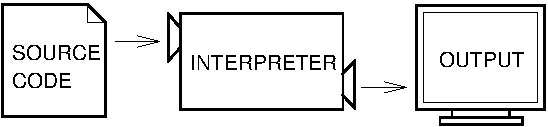
\includegraphics[scale=0.9]{figs/interpret.pdf}}
\caption{Ένας διερμηνέας επεξεργάζεται το πρόγραμμα
κομμάτι κομμάτι ή αλλιώς διαβάζει γραμμές και εκτελεί υπολογισμούς.}
\label{fig.interpret}
\end{figure}

Ένας μεταγλωττιστής διαβάζει το πρόγραμμα και το μεταφράζει ολόκληρο
πριν ξεκινήσει να τρέχει το πρόγραμμα.  Σε αυτό το πλαίσιο, το
πρόγραμμα υψηλού επιπέδου ονομάζεται {\bf πηγαίος κώδικας} (source code), και το
μεταφρασμένο πρόγραμμα ονομάζεται {\bf αντικειμενικός κώδικας} (object code) ή {\bf εκτελέσιμο} (executable). Όταν ένα πρόγραμμα μεταγλωττιστεί, μπορείτε να το εκτελέσετε επανειλημμένα
χωρίς περαιτέρω μετάφραση.

Εικόνα~\ref{fig.compile} δείχνει τη δομή ενός μεταγλωττιστή.

\begin{figure}
\centerline
{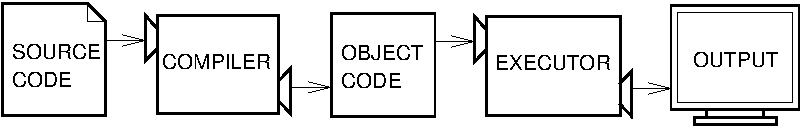
\includegraphics[scale=0.9]{figs/compile.pdf}}
\caption{Ένας μεταγλωττιστής μετατρέπει τον πηγαίο κώδικα σε αντικειμενικό κώδικα, ο οποίος τρέχει από έναν εκτελεστή υλικού.}
\label{fig.compile}
\end{figure}

 Η  Python  θεωρείτε μία διερμηνευμένη γλώσσα επειδή τα προγράμματά της
εκτελούνται από έναν διερμηνέα.  Υπάρχουν δύο τρόποι χρήσης του διερμηνέα: {\bf διαδραστική λειτουργία} 
(interactive mode) και {\bf σεναριακή λειτουργία} (script mode).  Στην διαδραστική
λειτουργία, πληκτρολογούμε προγράμματα σε Python και ο διερμηνέας εμφανίζει το αποτέλεσμα:

\index{interactive mode}
\index{script mode}

\begin{verbatim}

>>> 1 + 1
2
\end{verbatim}
%
 Το σύμβολο, \verb">>>", είναι ο {\bf προτροπέας} (prompt) που χρησιμοποιεί ο διερμηνέας 
για να υποδείξει ότι είναι έτοιμος.  Αν πληκτρολογήσετε {\tt 1 + 1}, ο διερμηνέας απαντάει {\tt 2}.
\index{prompt}

Εναλλακτικά, μπορείτε να αποθηκεύσετε κώδικα σε ένα αρχείο και να χρησιμοποιήσετε
το διερμηνέα για να εκτελέσει τα περιεχόμενα του αρχείου, το οποίο ονομάζεται 
{\bf σενάριο} (script).  Κατά παράδοση, τα σενάρια στην Python έχουν ονόματα με
κατάληξη {\tt .py}.
\index{script}

Για να εκτελεστεί το σενάριο πρέπει να δώσετε στο διερμηνέα το όνομα
του φακέλου.  Εάν έχετε ένα σενάριο με όνομα {\tt dinsdale.py} 
και δουλεύετε σε ένα παράθυρο εντολών  UNIX θα πρέπει πληκτρολογήσετε 
{\tt python dinsdale.py}.  Σε άλλα περιβάλλοντα ανάπτυξης, οι λεπτομέρειες
εκτέλεσης των σεναρίων είναι διαφορετικές.  Μπορείτε να βρείτε οδηγίες για
το περιβάλλον σας στην ιστοσελίδα της  Python \url{http://python.org}.

\index{testing!interactive mode}

 Όταν δουλεύετε στην διαδραστική λειτουργία σας βοηθάει να εξετάζετε
μικρά κομμάτια κώδικα επειδή μπορείτε να τα πληκτρολογήσετε και να εκτελεστούν
άμεσα.  Αλλά για κάτι παραπάνω από λίγες γραμμές, θα πρέπει να αποθηκεύσετε τον
κώδικά σας σαν σενάριο ώστε να μπορείτε να τον τροποποιήσετε και να το εκτελέσετε
στο μέλλον.


\section{ Τι είναι ένα πρόγραμμα}

Ένα {\bf πρόγραμμα} είναι μία ακολουθία εντολών η οποία προσδιορίζει
πως θα εκτελεστεί ένας υπολογισμός.  Αυτός ο υπολογισμός μπορεί να είναι
κάτι μαθηματικό, όπως το να λύνεις ένα σύστημα εξισώσεων ή το να βρίσκεις
τις ρίζες ενός πολυωνύμου, αλλά επίσης μπορεί να είναι ένας συμβολικός
υπολογισμός, όπως το να ψάχνεις και να αντικαθιστάς κείμενο μέσα σε ένα
έγγραφο ή (περιέργως) να μεταγλωττίζεις ένα πρόγραμμα.

\index{program}

Οι λεπτομέρειες είναι διαφορετικές από γλώσσα σε γλώσσα αλλά μερικές βασικές
εντολές εμφανίζονται σχεδόν σε όλες:

\begin{description}
\item[είσοδος:]   Εισαγωγή δεδομένων από το πληκτρολόγιο, ένα αρχείο, ή οποιαδήποτε
άλλη συσκευή.

\item[έξοδος:]   Εμφάνιση δεδομένων στην οθόνη ή αποστολή σε κάποιο αρχείο
ή συσκευή.

\item[μαθηματικά:]   Εκτέλεση βασικών μαθηματικών πράξεων όπως πρόσθεση και
πολλαπλασιασμός.

\item[εκτέλεση υπό συνθήκη:]   Έλεγχος συγκεκριμένων συνθηκών και εκτέλεση Ελέγχονται κατάλληλου κώδικα.

\item[επανάληψη:]   Εκτέλεση κάποιας ενέργειας κατ'επανάληψη με κάποια παραλλαγή.

\end{description}

Είτε το πιστεύετε είτε όχι, λίγο πολύ αυτό είναι όλο.  Κάθε πρόγραμμα
που έχετε χρησιμοποιήσει, ανεξάρτητα από το πόσο περίπλοκο ήταν,
απαρτίζεται από εντολές που μοιάζουν λίγο πολύ όπως αυτές.  Έτσι
μπορείτε να φανταστείτε τον προγραμματισμό σαν μία διαδικασία κατά
την οποία σπάμε μία μεγάλη και πολύπλοκη εργασία σε όλο και μικρότερες
υποδιεργασίες μέχρις ότου οι υποδιεργασίες να είναι αρκετά απλές για
να εκτελεστούν με μία από αυτές τις βασικές εντολές.
 \index{algorithm}

Αυτό μπορεί να είναι λίγο ασαφές αλλά θα επανέλθουμε σε αυτό το θέμα
όταν θα μιλήσουμε για αλγόριθμους.


\section{Τι είναι η αποσφαλμάτωση;}
\index{debugging}
\index{bug}
Ο προγραμματισμός είναι επιρρεπής σε λάθη.  Για ανεξήγητους λόγους
τα λάθη στον προγραμματισμό ονομάζονται στα αγγλικά {\bf bugs} 
ενώ στα ελληνικά σφάλματα και η διαδικασία εντοπισμού τους ονομάζεται
{\bf debugging}  ή αποσφαλμάτωση στα ελληνικά.

\index{debugging}
\index{bug}

Τρία είδη λαθών μπορεί να συμβούν σε ένα πρόγραμμα: συντακτικά λάθη,
λάθη χρόνου εκτέλεσης και λογικά λάθη. Είναι χρήσιμο να γίνει διάκριση
μεταξύ τους προκειμένου να εντοπίζονται γρηγορότερα.

\subsection{Συντακτικά λάθη}
\index{syntax error}
\index{error!syntax}
\index{error message}

Η Python μπορεί να εκτελέσει ένα πρόγραμμα μόνο εάν
έχει σωστή σύνταξη, διαφορετικά ο διερμηνέας εμφανίζει μήνυμα
λάθους.  Η {\bf σύνταξη} αφορά τη δομή ενός προγράμματος και τους
κανόνες αυτής της δομής.\index{syntax} 
Για παράδειγμα, οι παρενθέσεις πρέπει να είναι πάντα ζεύγη,
έτσι το {\tt (1 + 2)} είναι σωστό, αλλά το {\tt 8)} είναι ένα
{\bf συντακτικό λάθος} (syntax error).

\index{parentheses!matching}
\index{syntax}
\index{cummings, e. e.}

Στις γλώσσες που χρησιμοποιούμε για επικοινωνία (Ελληνικά, Αγγλικά, Γαλλικά) οι αναγνώστες δέχονται τα περισσότερα συντακτικά λάθη και για αυτό μπορούμε να διαβάζουμε την ποίηση του  e. e. cummings χωρίς να αραδιάζουμε μηνύματα λάθους.  Η Python όμως δεν
είναι τόσο επιεικής.  Εάν υπάρχει έστω και ένα συντακτικό λάθος
οπουδήποτε μέσα στο πρόγραμμα, η  Python  θα εμφανίσει ένα
μήνυμα λάθους και θα σταματήσει χωρίς να μπορείτε να τρέξετε
το πρόγραμμα.  Κατά τη διάρκεια των πρώτων εβδομάδων της προγραμματιστικής
σας καριέρας, πιθανότατα θα ξοδέψετε πολύ χρόνο στον εντοπισμό συντακτικών
λαθών.  Όσο αποκτάτε εμπειρία θα κάνετε λιγότερα λάθη και θα τα εντοπίζετε
γρηγορότερα.

\subsection{Λάθη χρόνου εκτέλεσης}
\label{runtime}

Ο δεύτερος τύπος λαθών είναι τα {\bf λάθη χρόνου εκτέλεσης} (runtime errors), ονομάζονται
έτσι επειδή τα λάθη δεν εμφανίζονται μέχρις ότου αρχίσει να τρέχει το πρόγραμμα. 
Αυτά τα λάθη ονομάζονται επίσης {\bf εξαιρέσεις} (exceptions) επειδή συνήθως
υποδεικνύουν ότι κάτι σημαντικό (και κακό) έχει συμβεί.
\index{runtime error}
\index{error!runtime}
\index{exception}
\index{safe language}
\index{language!safe}

Τα λάθη χρόνου εκτέλεσης είναι σπάνια στα απλά προγράμματα που θα δείτε
στα πρώτα κεφάλαια, έτσι ίσως πάρει λίγο χρόνο μέχρι να συναντήσετε ένα.

\subsection{Λογικά λάθη}
\index{semantics}
\index{semantic error}
\index{error!semantic}
\index{error message}

Ο τρίτος τύπος λάθους είναι τα {\bf λογικά λάθη} (semantic errors).  Εάν υπάρχει ένα λογικό
λάθος στο πρόγραμμά σας θα τρέξει επιτυχώς από την άποψη ότι ο υπολογιστής
δεν θα παράξει κανένα μήνυμα λάθους, αλλά δεν θα κάνει το σωστό. Θα
κάνει κάτι διαφορετικό.  Συγκεκριμένα, θα κάνει αυτό που του είπατε να
κάνει.

Το πρόβλημα είναι ότι το πρόγραμμα που γράψατε δεν είναι το πρόγραμμα
που θέλατε να γράψετε.  Το νόημα του προγράμματος (η σημασιολογία του)
είναι λάθος.  Η αναγνώριση λογικών λαθών μπορεί να είναι δύσκολη γιατί
απαιτεί να δουλέψετε προς τα πίσω κοιτάζοντας την έξοδο του προγράμματος
προσπαθώντας να καταλάβετε τι συμβαίνει.

\subsection{Πειραματική αποσφαλμάτωση}

Μία από τις πιο σημαντικές ικανότητες που θα αποκτήσετε είναι
η αποσφαλμάτωση.  Παρόλο που μπορεί να είναι μια επίπονη διαδικασία,
η αποσφαλμάτωση είναι ένα από τα πιο πνευματικώς πλούσια, προκλητικά
και ενδιαφέροντα μέρη του προγραμματισμού.

\index{experimental debugging}
\index{debugging!experimental}

Υπό μία έννοια, η αποσφαλμάτωση είναι σαν την δουλειά του ντετέκτιβ.  
Έρχεστε αντιμέτωποι με ενδείξεις, και πρέπει να συμπεράνετε από ποιες
διαδικασίες και συμβάντα προκύπτουν τα αποτελέσματα που βλέπετε.

Η αποσφαλμάτωση μοιάζει επίσης σαν μία πειραματική επιστήμη.  Από τη στιγμή
που έχετε μία ιδέα για το τι πηγαίνει λάθος, τροποποιείτε το πρόγραμμα και
ξαναδοκιμάζετε.  Εάν η υπόθεσή σας ήταν σωστή, τότε μπορείτε να προβλέψετε
το αποτέλεσμα της τροποποίησης και να είστε ένα βήμα πιο κοντά σε ένα
λειτουργικό πρόγραμμα.  Εάν η υπόθεσή σας ήταν λανθασμένη, πρέπει να κάνετε
μία νέα υπόθεση.  Όπως έχει τονίσει ο  Sherlock Holmes, "   Όταν έχετε
αποκλείσει το αδύνατο, οτιδήποτε μένει, όσο απίθανο και αν είναι, πρέπει να
είναι η αλήθεια ". (A. Conan Doyle, {\em The Sign of Four})
\index{Holmes, Sherlock}
\index{Doyle, Arthur Conan}

 Για μερικούς ανθρώπους, ο προγραμματισμός και η αποσφαλμάτωση είναι το ίδιο
πράγμα.  Δηλαδή, ο προγραμματισμός είναι η διαδικασία της σταδιακής
αποσφαλμάτωσης ενός προγράμματος έως ότου κάνει αυτό που θέλετε.   
Η γενική ιδέα είναι ότι θα πρέπει να ξεκινάτε με ένα πρόγραμμα το
οποίο κάνει "κάτι" και να κάνετε μικρές τροποποιήσεις, αποσφμαλματώνοντάς τες
προχωρώντας, έτσι ώστε να έχετε πάντα ένα λειτουργικό πρόγραμμα.  

Για παράδειγμα, το  Linux  είναι ένα λειτουργικό σύστημα το οποίο
περιέχει χιλιάδες γραμμές κώδικα, αλλά ξεκίνησε σαν ένα απλό πρόγραμμα
το οποίο ο  Linus Torvalds  χρησιμοποιούσε για να εξερευνήσει
το ολοκληρωμένο  Intel 80386.   Σύμφωνα με τον  Larry Greenfield,
 "Μία από τις πρώτες εργασίες του  Linus  ήταν ένα πρόγραμμα
το οποίο θα ανέστρεφε την εκτύπωση από ΑΑΑΑ σε ΒΒΒΒ.  Αυτό αργότερα εξελίχθηκε
στο  Linux."  ({\em The Linux Users' Guide} Beta Version 1).

\index{Linux}
 Τα επόμενα κεφάλαια θα κάνουν περισσότερες υποδείξεις σχετικά με την αποσφαλμάτωση και
άλλες προγραμματιστικές πρακτικές.


\section{Φυσικές και τυπικές γλώσσες}
\index{formal language}
\index{natural language}
\index{language!formal}
\index{language!natural}

Οι {\bf φυσικές γλώσσες} είναι οι γλώσσες που μιλούν οι άνθρωποι,
όπως τα Αγγλικά, τα Ισπανικά και τα Γαλλικά.  Δεν έχουν σχεδιαστεί
από τους ανθρώπους (παρόλο που οι άνθρωποι προσπαθούν να επιβάλουν
κάποια τάξη σε αυτές), έχουν εξελιχθεί φυσικά.

Οι {\bf τυπικές γλώσσες} (formal) είναι γλώσσες που έχουν σχεδιαστεί από ανθρώπους
για συγκεκριμένες εφαρμογές.  Για παράδειγμα, η σημειογραφία που χρησιμοποιούν
οι μαθηματικοί είναι μια τυπική γλώσσα η οποία είναι ιδιαίτερα καλή στο
να δείχνει τις σχέσεις μεταξύ αριθμών και συμβόλων.  Οι χημικοί χρησιμοποιούν
μία τυπική γλώσσα για να αναπαραστήσουν τη χημική δομή των μορίων. Και το πιο
σημαντικό:

\begin{quote}
{\bf Οι προγραμματιστικές γλώσσες είναι τυπικές γλώσσες οι οποίες έχουν σχεδιαστεί
για να εκφράζουν υπολογισμούς.}
\end{quote}

Οι τυπικές γλώσσες τείνουν να έχουν αυστηρούς κανόνες σύνταξης.  Για
παράδειγμα,
$3 + 3 = 6$  είναι μία συντακτικά σωστή μαθηματική έκφραση, αλλά αυτή
$3 + = 3 \mbox{\$} 6$ δεν είναι.
$H_2O$ είναι ένας συντακτικά σωστός
χημικός τύπος, αλλά αυτός $_2Zz$ δεν είναι.

Οι κανόνες σύνταξης είναι δύο τύπων, αυτοί που αφορούν τα {\bf σύμβολα} (tokens)
και αυτοί που αφορούν τη {\bf δομή} (structure). Τα σύμβολα είναι τα βασικά στοιχεία της γλώσσας όπως λέξεις, αριθμοί και χημικά στοιχεία.  Ένα από τα προβλήματα με το
$3 + = 3 \mbox{\$} 6$ είναι ότι το \( \$ \) δεν είναι ένα έγκυρο
σύμβολο στα μαθηματικά (τουλάχιστον απ' όσο γνωρίζω).  Παρομοίως, το
$_2Zz$ δεν είναι έγκυρο επειδή δεν υπάρχει στοιχείο με την συντομογραφία
$Zz$.

\index{token}
\index{structure}

Ο δεύτερος τύπος συντακτικού κανόνα αφορά τη δομή μίας έκφρασης,
δηλαδή τον τρόπο με τον οποίο έχουν διαταχθεί τα σύμβολα.  
Η έκφραση $3 + = 3$ είναι λάθος γιατί παρόλο που το $+$ και το
$=$ είναι έγκυρα σύμβολα, δεν μπορείτε να έχετε το ένα ακριβώς
μετά το άλλο.  Παρομοίως, σε ένα χημικό τύπο ο δείκτης μπαίνει
μετά το όνομα του στοιχείου, όχι πριν.

Όταν διαβάζετε μία πρόταση στα Αγγλικά ή μία έκφραση σε μία τυπική
γλώσσα, πρέπει να καταλάβετε ποια είναι η δομή της πρότασης
(παρόλο που σε μια φυσική γλώσσα το κάνετε υποσυνείδητα).  Αυτή
η διαδικασία ονομάζεται συντακτική ανάλυση.
\index{parse}

Για παράδειγμα, όταν ακούτε την πρόταση, "Το νόμισμα έπεσε,"
καταλαβαίνετε ότι "το νόμισμα" είναι το αντικείμενο και το "έπεσε"
είναι το κατηγορούμενο.  Μόλις αναλύσετε μία πρόταση, μπορείτε
να καταλάβετε τι σημαίνει ή αλλιώς τη σημασιολογία της πρότασης.  
Υποθέτοντας ότι γνωρίζετε τι είναι το νόμισμα και τι σημαίνει το ότι
πέφτει, θα καταλάβετε τον υπαινιγμό της πρότασης.

Παρόλο που οι επίσημες και οι τυπικές γλώσσες έχουν πολλά κοινά
χαρακτηριστικά---σύμβολα, δομή, συντακτικό και σημασιολογία---υπάρχουν
κάποιες διαφορές:
\index{ambiguity}
\index{redundancy}
\index{literalness}

\begin{description}

\item[ασάφεια:] Οι φυσικές γλώσσες είναι γεμάτες ασάφεια την οποία
οι άνθρωποι αντιμετωπίζουν με βάση τα συμφραζόμενα και άλλες πληροφορίες.  
Οι τυπικές γλώσσες έχουν σχεδιαστεί για να είναι σχεδόν ή πλήρως σαφείς,
το οποίο σημαίνει ότι οποιαδήποτε έκφραση έχει ακριβώς μία ερμηνεία,
ανεξαρτήτως περιεχομένου.

\item[πλεονασμός:] Προκειμένου να επιτύχουμε σαφήνεια και να μειώσουμε
τις παρεξηγήσεις, οι φυσικές γλώσσες χρησιμοποιούν πολλούς πλεονασμούς.  
Σαν αποτέλεσμα, είναι συχνά φλύαρες.  Οι τυπικές γλώσσες είναι λιγότερο
πλεονάζουσες και περισσότερο συνοπτικές.

\item[μεταφορά:] Οι φυσικές γλώσσες είναι γεμάτες από ιδιωματισμούς
και μεταφορές.  Εάν πω, "Το νόμισμα έπεσε" πιθανώς δεν υπάρχει νόμισμα
και τίποτα δεν έχει πέσει (αυτός ο ιδιωματισμός σημαίνει ότι κάποιος
συνειδητοποίησε κάτι μετά από μία περίοδο σύγχυσης).  Οι τυπικές γλώσσες
εννοούν αυτό ακριβώς που λένε.

\end{description}

Οι άνθρωποι που μεγάλωσαν μιλώντας μία φυσική γλώσσα (όλοι) είναι
συχνά δύσκολο να εξοικειωθούν με τις τυπικές γλώσσες.  Κατά κάποιον τρόπο,
η διαφορά ανάμεσα στην τυπική και στη φυσική γλώσσα είναι σαν τη διαφορά
ανάμεσα στην ποίηση και στον πεζό λόγο, αλλά ειδικότερα:
\index{poetry}
\index{prose}

\begin{description}

\item[Ποίηση:] Οι λέξεις χρησιμοποιούνται τόσο για τους ήχους τους
όσο και για τη σημασία τους, και ολόκληρο το ποίημα δημιουργεί μία
συναισθηματική αντίδραση.  Η ασάφεια δεν είναι μόνο σύνηθες φαινόμενο
αλλά συχνά σκόπιμη.

\item[Πεζός λόγος:] Η κυριολεκτική έννοια των λέξεων είναι περισσότερο
σημαντική, και η δομή συμβάλλει περισσότερο στο νόημα.  Ο πεζός λόγος
επιδέχεται περισσότερη ανάλυση από την ποίηση αλλά είναι συχνά
διφορούμενος.

\item[Προγράμματα:] Το νόημα ενός υπολογιστικού προγράμματος είναι
σαφές και κυριολεκτικό, και μπορεί να κατανοηθεί πλήρως μέσω της ανάλυσης
των συμβόλων και της δομής.

\end{description}

Αυτές είναι κάποιες υποδείξεις για το πώς να διαβάζετε προγράμματα (και άλλες
τυπικές γλώσσες).  Πρώτον, να θυμάστε ότι οι τυπικές γλώσσες είναι
περισσότερο πυκνογραμμένες από τις φυσικές γλώσσες, γι' αυτό παίρνει
περισσότερο να τις διαβάσουμε.  Επίσης η δομή είναι πολύ σημαντική,
οπότε συνήθως δεν είναι καλή ιδέα να τις διαβάζουμε από την αρχή προς
το τέλος, από αριστερά στα δεξιά.  Αντί αυτού, πρέπει να μάθετε να αναλύετε
το πρόγραμμα στο μυαλό σας, αναγνωρίζοντας τα σύμβολα και ερμηνεύοντας
τη δομή.  Τελικά, οι λεπτομέρειες μετράνε.  Μικρά λάθη στο συλλαβισμό και
στη στίξη, τα οποία δεν δημιουργούν σοβαρό πρόβλημα στις φυσικές γλώσσες,
μπορούν να κάνουν μεγάλη διαφορά σε μία τυπική γλώσσα.


\section{Το πρώτο πρόγραμμα}
\label{hello}
\index{Hello, World}

Κατά παράδοση, το πρώτο πρόγραμμα που γράφετε σε μία νέα
γλώσσα ονομάζεται ''Hello, World!'' επειδή το μόνο που κάνει
είναι να εμφανίζει τις λέξεις ''Hello, World''. Στην Python
είναι κάπως έτσι:

\begin{verbatim}
print 'Hello, World!'
\end{verbatim}
%

Αυτό είναι ένα παράδειγμα μίας {\bf δήλωσης εκτύπωσης}, η οποία
στην πραγματικότητα δεν εκτυπώνει κάτι στο χαρτί αλλά εμφανίζει μία
τιμή στην οθόνη. Σε αυτή την περίπτωση το αποτέλεσμα είναι οι λέξεις:

\begin{verbatim}
Hello, World!
\end{verbatim}
%

Τα εισαγωγικά μέσα στο πρόγραμμα σηματοδοτούν την αρχή και το τέλος
του κειμένου που θα εμφανιστεί και δεν φαίνονται στο αποτέλεσμα.

\index{quotation mark}
\index{print statement}
\index{statement!print}

Στην Python 3, η σύνταξη για εκτύπωση είναι λίγο διαφορετική:

\begin{verbatim}
print('Hello, World!')
\end{verbatim}
%
Οι παρενθέσεις υποδηλώνουν ότι η {\tt print} είναι μία
συνάρτηση. Θα δούμε τις συναρτήσεις στο Κεφάλαιο~\ref{funcchap}.

\index{function} \index{print function} \index{Python 3}

Στη συνέχεια αυτού του βιβλίου θα χρησιμοποιήσουμε την έκφραση print της Python2.  
Εάν χρησιμοποιείτε την  Python 3  θα πρέπει να την προσαρμόζετε.  
Αλλά εκτός αυτού δεν υπάρχουν πολλές διαφορές για τις οποίες θα
πρέπει να ανησυχούμε.


\section{Αποσφαλμάτωση}
\index{debugging}
Είναι προτιμότερο να διαβάζετε αυτό το βιβλίο μπροστά από έναν υπολογιστή
έτσι ώστε να μπορείτε να δοκιμάζετε τα παραδείγματα όσο προχωράτε.  Μπορείτε
να τρέξετε τα περισσότερα από τα παραδείγματα σε διαδραστική λειτουργία αλλά αν 
βάζατε τον κώδικα μέσα σε ένα σενάρια τότε θα ήταν ευκολότερο να πειραματιστείτε.

Κάθε φορά που πειραματίζεστε με ένα νέο χαρακτηριστικό της γλώσσας, θα πρέπει να δοκιμάζετε
να κάνετε λάθη. Για παράδειγμα, τι θα συμβεί στο πρόγραμμα ''Hello, world!'' αν δεν βάλετε ένα από τα εισαγωγικά; Εάν δεν βάλετε κανένα από τα δύο; Εάν γράψετε λάθος την {\tt print};
\index{error message}

Αυτό το είδος πειραματισμού σας βοηθάει να θυμάστε τι διαβάζετε και επίσης
σας βοηθάει στην αποσφαλμάτωση, επειδή θα μάθετε τι σημαίνουν τα μηνύματα
λάθους.  Είναι προτιμότερο να κάνετε εσκεμμένα λάθη τώρα παρά αργότερα κατά
λάθος.

Μερικές φορές, ο προγραμματισμός και ιδιαίτερα η αποσφαλμάτωση  μπορεί να προκαλέσουν 
έντονα συναισθήματα. Εάν ταλαιπωρείστε με ένα δύσκολο σφάλμα τότε μπορεί να
νιώσετε Θυμό, αποθάρρυνση ή ακόμα και ντροπή.

Έχει αποδειχθεί ότι οι άνθρωποι αντιμετωπίζουν τους υπολογιστές
σαν να ήταν άνθρωποι.  Όταν λειτουργούν σωστά τους βλέπουμε σαν συνεργάτες αλλά 
όταν είναι "πεισματάρηδες" ή "αγενείς", τότε τους συμπεριφερόμαστε με τον
ίδιο τρόπο που θα συμπεριφερόμασταν σε αγενείς και πεισματάρηδες ανθρώπους
(Reeves and Nass, {\it The Media Equation: How People Treat Computers, Television, and New Media Like Real People and Places}).
\index{debugging!emotional response}
\index{emotional debugging}

Αν είστε προετοιμασμένοι για αυτές τις αντιδράσεις μπορείτε να
τις αντιμετωπίσετε.  Μία καλή λύση είναι να σκέφτεστε
τον υπολογιστή σαν ένα υπάλληλο με συγκεκριμένες δυνατότητες όπως
η ταχύτητα και η ακρίβεια και συγκεκριμένες αδυναμίες όπως η έλλειψη
συναίσθησης και η ανικανότητά τους να κατανοήσουν το γενικό νόημα.

Η δουλειά σας είναι να είστε ένας καλός διευθυντής: βρείτε τρόπους
να εκμεταλλευτείτε τις δυνατότητες και να μετριάσετε τις αδυναμίες.  
Επίσης, βρείτε τρόπους να χρησιμοποιήσετε τα συναισθήματά σας ώστε
να ασχοληθείτε με το πρόβλημα χωρίς να αφήσετε τις αντιδράσεις σας
να επηρεάσουν την ικανότητά σας να δουλεύετε αποδοτικά.

Το να μάθετε να αποσφαλματώνετε μπορεί να είναι απογοητευτικό
αλλά είναι μία σημαντική ικανότητα η οποία είναι χρήσιμη και για
πολλές δραστηριότητες πέραν του προγραμματισμού.  Στο τέλος κάθε
κεφαλαίου υπάρχει μία ενότητα αποσφαλμάτωσης όπως αυτή με τις
σκέψεις μου σχετικά με την αποσφαλμάτωση. Ελπίζω να βοηθήσουν!


\section{Ορολογία}

\begin{description}

\item[επίλυση προβλημάτων:]  Η διαδικασία τυποποίησης ενός προβλήματος,
	η εύρεση λύσης και η έκφραση της λύσης.
\index{problem solving}

\item[γλώσσα υψηλού επιπέδου:]  Μία γλώσσα προγραμματισμού όπως η 
	Python  που έχει σχεδιαστεί για να είναι εύκολη για τους ανθρώπους
	στην ανάγνωση και στη γραφή.
\index{high-level language}

\item[γλώσσα χαμηλού επιπέδου:]  Μία γλώσσα που έχει σχεδιαστεί για να είναι
	εύκολο να εκτελεστεί από έναν υπολογιστή, ονομάζεται επίσης "γλώσσα μηχανής" ή
	"συμβολική γλώσσα."
\index{low-level language}

\item[φορητότητα:]  Η ιδιότητα ενός προγράμματος να μπορεί να τρέξει σε
	σε διαφορετικούς υπολογιστές.
\index{portability}

\item[διερμηνεία:]  Να εκτελείς ένα πρόγραμμα γλώσσας υψηλού επιπέδου
	μεταφράζοντάς μία γραμμή κάθε φορά.
\index{interpret}

\item[μεταγλώττιση:]  Να μεταφράζεις ένα πρόγραμμα γραμμένο σε γλώσσα
	υψηλού επιπέδου σε γλώσσα χαμηλού επιπέδου κατευθείαν, προετοιμάζοντάς το
	για μετέπειτα εκτέλεση.
\index{compile}

\item[πηγαίος κώδικας:]  Ένα πρόγραμμα σε μία γλώσσα υψηλού επιπέδου
	προτού μεταγλωττιστεί.
\index{source code}

\item[αντικείμενος κώδικας:]  Η έξοδος του μεταγλωττιστή αφού μετατρέψει
	το πρόγραμμα.
\index{object code}

\item[εκτελέσιμο:]  Μία άλλη ονομασία του αντικείμενου κώδικα ο οποίος
	είναι έτοιμος για εκτέλεση.
\index{executable}

\item[προτροπέας:] Οι χαρακτήρες που εμφανίζονται από το διερμηνέα για να 
	υποδηλώσουν ότι είναι έτοιμος να δεχτεί την είσοδο από το χρήστη.
\index{prompt}

\item[σενάριο:] Ένα πρόγραμμα αποθηκευμένο σε ένα αρχείο (συνήθως προς
	διερμηνεία).
\index{script}

\item[διαδραστική λειτουργία:] Ένας τρόπος χρήσης του διερμηνέα της
	 Python  πληκτρολογώντας εντολές και εκφράσεις στον προτροπέα.
\index{interactive mode}

\item[σεναριακή λειτουργία:] Ένας τρόπος χρήσης του διερμηνέα της 
	Python  που διαβάζει και εκτελεί εκφράσεις από ένα σενάριο.
\index{script mode}

\item[πρόγραμμα:] Ένα σύνολο εντολών που ορίζει έναν υπολογισμό.
\index{program}

\item[αλγόριθμος:]  Μία γενική διαδικασία για την επίλυση μιας κατηγορίας
	προβλημάτων.
\index{algorithm}

\item[σφάλμα:]  Ένα λάθος σε κάποιο πρόγραμμα.
\index{bug}

\item[αποσφαλμάτωση:]  Η διαδικασία εύρεσης και απομάκρυνσης οποιουδήποτε
	εκ των τριών τύπων προγραμματιστικών σφαλμάτων.
\index{debugging}

\item[συντακτικό:]  Η δομή ενός προγράμματος.
\index{syntax}

\item[συντακτικό λάθος:]  Ένα λάθος σε ένα πρόγραμμα το οποίο το καθιστά
	αδύνατο να αναλυθεί (και επομένως αδύνατον να διερμηνευτεί).
\index{syntax error}

\item[εξαίρεση:]  Ένα λάθος το οποίο ανακύπτει κατά την εκτέλεση του προγράμματος.
\index{exception}

\item[σημασιολογία:]  Το νόημα ενός προγράμματος.
\index{semantics}

\item[σημασιολογικό λάθος:]   Ένα λάθος σε ένα πρόγραμμα όταν αυτό 
	κάνει κάτι διαφορετικό από αυτό που είχε σκοπό ο προγραμματιστής.
\index{semantic error}

\item[φυσική γλώσσα:]  Οποιαδήποτε από τις γλώσσες που μιλούν οι άνθρωποι
	η οποία έχει εξελιχθεί φυσικά.
\index{natural language}

\item[τυπική γλώσσα:]  Οποιαδήποτε από τις γλώσσες που έχουν σχεδιάσει
	οι άνθρωποι για συγκεκριμένους σκοπούς, όπως αναπαράσταση μαθηματικών
	ιδεών ή προγραμμάτων υπολογιστών.  Όλες οι γλώσσες προγραμματισμού είναι
	τυπικές γλώσσες.
\index{formal language}

\item[σύμβολο:]  Ένα από τα βασικά στοιχεία της συντακτικής δομής ενός
	προγράμματος, αντίστοιχο με τη λέξη σε μια φυσική γλώσσα.
\index{token}

\item[ανάλυση:] Να εξετάζεις ένα πρόγραμμα και να αναλύεις την συντακτική
	του δομή.
\index{parse}

\item[δήλωση εκτύπωσης:]  Μία εντολή που προκαλεί τον διερμηνέα της 
	Python  να εμφανίσει μία τιμή στην οθόνη.
\index{print statement}
\index{statement!print}


\end{description}


\section{Ασκήσεις}


\begin{exercise}
Χρησιμοποιήστε ένα φυλλομετρητή για να επισκεφθείτε την ιστοσελίδα της Python \url{http://python.org}.  
Αυτή η σελίδα περιέχει πληροφορίες σχετικά με την  Python 
και συνδέσμους οι οποίοι σχετίζονται με την  Python, 
και σας δίνει την δυνατότητα να αναζητήσετε την τεκμηρίωση της  Python.

 Για παράδειγμα, εάν πληκτρολογήσετε  {\tt print}  στο πεδίο της
αναζήτησης, ο πρώτος σύνδεσμος που εμφανίζεται είναι η τεκμηρίωση για αυτήν
την έκφραση.  Σε αυτό το σημείο ενδεχομένως να μην βγάζει νόημα όλο αυτό το κατεβατό, αλλά είναι καλό να ξέρετε που υπάρχει.
\\
\index{documentation}
\index{python.org}
\end{exercise}


\begin{exercise}
Εκκινήστε τον διερμηνέα της  Python  πληκτρολογήστε  {\tt help()} 
για να ξεκινήσει το διαδικτυακό εργαλείο βοήθειας.  Ή μπορείτε να πληκτρολογήσετε \verb"help('print')" για να πάρετε πληροφορίες σχετικές με την έκφραση {\tt print}.

Εάν αυτό το παράδειγμα δεν δουλεύει, ίσως χρειαστεί να εγκαταστήσετε επιπρόσθετη τεκμηρίωση της  Python  ή να θέσετε μία μεταβλητή περιβάλλοντος, οι λεπτομέρειες εξαρτώνται από το λειτουργικό σας σύστημα και την έκδοση της  Python. 
\\
\index{help utility}
\end{exercise}


\begin{exercise}
Εκκινήστε τον διερμηνέα της  Python  και χρησιμοποιήστε τον
σαν αριθμομηχανή.  Το συντακτικό της  Python  για μαθηματικές
πράξεις είναι σχεδόν το ίδιο με την τυπική μαθηματική σημειογραφία.  
Για παράδειγμα, τα σύμβολα {\tt +}, {\tt -} και {\tt /}
δηλώνουν πρόσθεση, αφαίρεση και διαίρεση, όπως θα περιμένατε.  
Το σύμβολο του πολλαπλασιασμού είναι {\tt *}.  

Εάν τρέξετε έναν αγώνα 10 χιλιομέτρων σε 43 λεπτά και 30 δευτερόλεπτα,
ποιος είναι ο μέσος χρόνος σας ανά μίλι ;  Ποια είναι η μέση σας ταχύτητα
σε μίλια ανά ώρα; (Σημείωση: ένα μίλι είναι 1,61 χιλιόμετρα).
\index{calculator}
\index{running pace}
\end{exercise}





\chapter{Μεταβλητές, εκφράσεις και δηλώσεις}

\section{Τιμές και τύποι}
\index{value}
\index{type}
\index{string}

Μία {\bf τιμή} είναι ένα από τα βασικά στοιχεία που κάνουν λειτουργικό 
ένα πρόγραμμα, όπως για παράδειγμα ένα γράμμα ή ένας αριθμός.  Οι τιμές που έχουμε δει μέχρι στιγμής είναι οι {\tt 1}, {\tt 2}, και \verb"'Hello, World!'".

Αυτές οι τιμές υπόκεινται σε διαφορετικούς τύπους:
το {\tt 2} είναι ακέραιος και το \verb"'Hello, World!'" είναι
μία συμβολοσειρά (ονομάζεται έτσι επειδή περιέχει μια "σειρά" από
σύμβολα (γράμματα). Μπορείτε (το ίδιο και ο διερμηνέας) να αναγνωρίσετε συμβολοσειρές, επειδή περικλείονται σε εισαγωγικά.
\index{quotation mark}

Αν δεν είστε σίγουροι για τον τύπο μιας τιμής, τότε μπορεί να σας τον υποδείξει ο  διερμηνέας:

\begin{verbatim}
>>> type('Hello, World!')
<type 'str'>
>>> type(17)
<type 'int'>
\end{verbatim}
%

Προφανώς, οι συμβολοσειρές ανήκουν στον τύπο {\tt str}
και οι ακέραιοι ανήκουν στον τύπο {\tt int}.  
Λιγότερο προφανές είναι όμως ότι οι αριθμοί με δεκαδικά ψηφία ανήκουν
σε ένα τύπο που ονομάζεται {\tt float}, επειδή αυτοί οι αριθμοί
παριστάνονται σε μία μορφή ονομαζόμενη  {\bf floating-point}.
\index{type}
\index{string type}
\index{type!str}
\index{int type}
\index{type!int}
\index{float type}
\index{type!float}

\begin{verbatim}
>>> type(3.2)
<type 'float'>
\end{verbatim}
%
Τι γίνεται με τιμές όπως η \verb"'17'" και η 
\verb"'3.2'"; Μοιάζουν με αριθμούς αλλά περικλείονται
σε εισαγωγικά όπως οι συμβολοσειρές.
\index{quotation mark}

\begin{verbatim}
>>> type('17')
<type 'str'>
>>> type('3.2')
<type 'str'>
\end{verbatim}
%

Είναι συμβολοσειρές.

Εάν πληκτρολογήσετε έναν μεγάλο ακέραιο τότε ίσως μπείτε στον πειρασμό
να χρησιμοποιήσετε κόμματα (ή τελείες) ανά τρία ψηφία, όπως για παράδειγμα
{\tt 1,000,000}.  Αυτός δεν είναι έγκυρος ακέραιος για την 
Python, αλλά γενικά είναι σωστό:

\begin{verbatim}
>>> 1,000,000
(1, 0, 0)
\end{verbatim}
%

Αυτό προφανώς δεν έχει καμία σχέση με αυτό που περιμέναμε!  Η 
Python  ερμηνεύει το  {\tt 1,000,000}  σαν μία ακολουθία
ακεραίων χωρισμένη με κόμματα.  Αυτό είναι το πρώτο παράδειγμα σημασιολογικού (λογικού) λάθους που βλέπουμε: ο κώδικας τρέχει χωρίς να παράγει κανένα μήνυμα
λάθους αλλά δεν κάνει αυτό που θέλαμε.
\index{semantic error}
\index{error!semantic}
\index{error message}



\section{Μεταβλητές}
\label{variables}
\index{variable}
\index{assignment statement}
\index{statement!assignment}
Ένα από τα πιο δυνατά χαρακτηριστικά μιας γλώσσας προγραμματισμού
είναι η ικανότητα να διαχειρίζεται {\bf μεταβλητές} (variables). Μία μεταβλητή είναι ένα όνομα που αναφέρεται σε μία τιμή.

Μία {\bf δήλωση εκχώρησης} (assignment statement) δημιουργεί νέες μεταβλητές και δίνει τιμές σε αυτές:

\begin{verbatim}
>>> message = 'And now for something completely different'
>>> n = 17
>>> pi = 3.1415926535897932
\end{verbatim}
%

Σε αυτό το παράδειγμα κάνουμε τρεις εκχωρήσεις τιμών. Η πρώτη εκχωρεί
μία συμβολοσειρά σε μία νέα μεταβλητή με όνομα {\tt message}, 
η δεύτερη δίνει στη {\tt n} την ακέραια τιμή {\tt 17} και
η τρίτη εκχωρεί την (κατά προσέγγιση) τιμή του $\pi$ στην {\tt pi}.
\index{state diagram}
\index{diagram!state}

Ο πιο συνηθισμένος τρόπος αναπαράστασης των μεταβλητών σε χαρτί είναι να γράψετε το όνομα της μεταβλητής με ένα βελάκι το οποίο θα δείχνει την τιμή της. Αυτός ο τρόπος απεικόνισης ονομάζεται {\bf διάγραμμα κατάστασης} (state diagram) γιατί δείχνει την κατάσταση της κάθε μεταβλητής. Το σχήμα~\ref{fig.state2} δείχνει το αποτέλεσμα του προηγούμενου παραδείγματος.

\begin{figure}
\centerline
{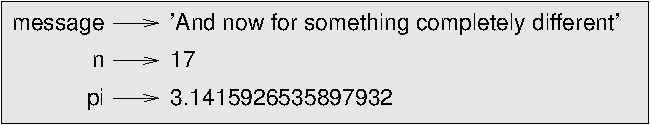
\includegraphics[scale=0.8]{figs/state2.pdf}}
\caption{Διάγραμμα Κατάστασης.}
\label{fig.state2}
\end{figure}

Ο τύπος της μεταβλητής είναι ίδιος με τον τύπο της τιμής στην οποία αναφέρεται.

\begin{verbatim}
>>> type(message)
<type 'str'>
>>> type(n)
<type 'int'>
>>> type(pi)
<type 'float'>
\end{verbatim}
\vfill
\begin{exercise}

Εάν πληκτρολογήσετε έναν ακέραιο που έχει στην αρχή μηδέν, ενδεχομένως
να προκύψει σφάλμα λόγω σύγχυσης στο διερμηνέα:

\begin{verbatim}
>>> zipcode = 02492
                  ^
SyntaxError: invalid token
\end{verbatim}

Άλλα νούμερα φαίνεται να δουλεύουν, αλλά τα αποτελέσματα είναι παράξενα:

\begin{verbatim}
>>> zipcode = 02132
>>> zipcode
1114
\end{verbatim}

Μπορείτε να καταλάβετε τι συμβαίνει ;  Σημείωση: εμφανίστε τις
τιμές  {\tt 01}, {\tt 010}, {\tt 0100}  και  {\tt 01000}.
\index{octal}
\end{exercise}



\section{Ονόματα μεταβλητών και λέξεις κλειδιά}
\index{keyword}

Γενικά, οι προγραμματιστές επιλέγουν ονόματα για τις μεταβλητές τους
τα οποία έχουν κάποιο νόημα (τεκμηριώνουν για ποιο λόγο χρησιμοποιείται
η μεταβλητή).

Τα ονόματα των μεταβλητών μπορούν να είναι αυθαίρετα μεγάλα και 
μπορούν να περιέχουν και γράμματα και νούμερα αλλά πρέπει να
ξεκινάνε με ένα γράμμα.  Είναι έγκυρο να χρησιμοποιούμε κεφαλαία
γράμματα αλλά είναι προτιμότερο να ξεκινάτε τα ονόματα των μεταβλητών
με πεζά (θα δείτε αργότερα γιατί).

Η κάτω παύλα (\verb"_") μπορεί να χρησιμοποιηθεί σε κάποιο όνομα και 
είναι ιδιαίτερα χρήσιμη σε ονόματα με πολλές λέξεις όπως το 
\verb"my_name" ή το \verb"airspeed_of_unladen_swallow".

\index{underscore character}

Εάν δώσετε σε μία μεταβλητή λάθος όνομα τότε θα παραχθεί συντακτικό λάθος:

\begin{verbatim}
>>> 76trombones = 'big parade'
SyntaxError: invalid syntax
>>> more@ = 1000000
SyntaxError: invalid syntax
>>> class = 'Advanced Theoretical Zymurgy'
SyntaxError: invalid syntax
\end{verbatim}
%
 Το {\tt 76trombones} είναι λάθος γιατί δεν ξεκινάει με γράμμα.  
Το {\tt more@} είναι λάθος γιατί περιέχει ένα μη έγκυρο χαρακτήρα ({\tt
@}). Αλλά γιατί το {\tt class} είναι λάθος;

Αποδεικνύεται ότι το {\tt class} είναι μία από τις {\bf λέξεις κλειδιά} (keywords) της 
Python. Ο διερμηνέας χρησιμοποιεί λέξεις κλειδιά για να αναγνωρίσει τη δομή ενός
προγράμματος και για αυτόν το λόγο δεν μπορούν χρησιμοποιηθούν για ονόματα μεταβλητών.

\index{keyword}

Η Python 2 έχει 31 λέξεις κλειδιά.

\begin{verbatim}
and       del       from      not       while
as        elif      global    or        with
assert    else      if        pass      yield
break     except    import    print
class     exec      in        raise
continue  finally   is        return
def       for       lambda    try
\end{verbatim}
%

Στην Python 3 το {\tt exec} δεν είναι πλέον λέξη κλειδί αλλά είναι το 
{\tt nonlocal}.

Καλό θα ήταν να έχετε αυτή τη λίστα εύχερη σε περίπτωση που ο διερμηνέας παραπονεθεί για μία από τις μεταβλητές σας και δεν ξέρετε γιατί, κοιτάξτε αν βρίσκεται σε αυτή τη λίστα.


\section{Τελεστές και τελεστέοι}
\index{operator, arithmetic}
\index{arithmetic operator}
\index{operand}
\index{expression}

Οι {\bf τελεστές} είναι ειδικά σύμβολα τα οποία αναπαριστούν υπολογισμούς
όπως η πρόσθεση και ο πολλαπλασιασμός. Οι τιμές στις οποίες εφαρμόζεται
ο τελεστής ονομάζονται {\bf τελεστέοι}.

Οι τελεστές  {\tt +}, {\tt -}, {\tt *}, {\tt /}  και  {\tt **}
εκτελούν πρόσθεση, αφαίρεση, πολλαπλασιασμό, διαίρεση και ύψωση σε
δύναμη:


\begin{verbatim}
20+32   hour-1   hour*60+minute   minute/60   5**2   (5+9)*(15-7)
\end{verbatim}
%

Σε κάποιες άλλες γλώσσες, για την ύψωση σε δύναμη χρησιμοποιείται το
σύμβολο \verb"^" αλλά στην Python είναι δυαδικός
τελεστής και ονομάζεται XOR. Σε αυτό το βιβλίο δεν θα επεκταθούμε
στους δυαδικούς τελεστές αλλά μπορείτε να διαβάσετε για αυτούς στην
διεύθυνση \url{http://wiki.python.org/moin/BitwiseOperators}.
\index{bitwise operator}
\index{operator!bitwise}

Στην Python, ο τελεστής της διαίρεσης μπορεί να μην κάνει
αυτό που θα περιμένατε:

\begin{verbatim}
>>> minute = 59
>>> minute/60
0
\end{verbatim}
%

Η τιμή του {\tt minute} είναι 59 και στα συμβατικά μαθηματικά
το 59 διαιρούμενο με το 60 μας δίνει 0.98333 και όχι 0.  Ο λόγος που
συμβαίνει αυτό είναι ότι η  Python  εκτελεί ακέραια διαίρεση.  
Όταν και οι δύο τελεστέοι είναι ακέραιοι αριθμοί τότε το αποτέλεσμα θα είναι
επίσης ακέραιος αριθμός γιατί η ακέραια διαίρεση κόβει το κλασματικό
τμήμα.  Έτσι, σε αυτό το παράδειγμα το αποτέλεσμα στρογγυλοποιείται
στο μηδέν.


Στην Python 3 το αποτέλεσμα της διαίρεσης είναι {\tt float} και   
ο νέος τελεστής για την ακέραια διαίρεση είναι {\tt //}.
\index{Python 3}
\index{floor division}
\index{floating-point division}
\index{division!floor}
\index{division!floating-point}

Εάν κάποιος από τους τελεστέους είναι αριθμός κινητής υποδιαστολής τότε 
η Python εκτελεί κλασματική διαίρεση και το αποτέλεσμα είναι
{\tt float}:

\begin{verbatim}
>>> minute/60.0
0.98333333333333328
\end{verbatim}


\section{Εκφράσεις και δηλώσεις}

Μία {\bf έκφραση} είναι ένας συνδυασμός από τιμές, μεταβλητές και τελεστές.  
Μία τιμή από μόνη της θεωρείται σαν μία έκφραση, το ίδιο και μία
μεταβλητή. Έτσι όλες οι ακόλουθες εκφράσεις είναι έγκυρες
(υποθέτοντας ότι έχει ανατεθεί τιμή στη μεταβλητή {\tt x}): 				
\index{expression}
\index{evaluate}

\begin{verbatim}
17
x
x + 17
\end{verbatim}
%

Μία δήλωση είναι μία μονάδα κώδικα την οποία ο διερμηνέας της Python 
μπορεί να εκτελέσει.  Έχουμε δει δύο τύπους δηλώσεων: την εκτύπωση
και την εκχώρηση.

Στην πράξη μία έκφραση είναι ταυτόχρονα και δήλωση αλλά ίσως είναι πιο
απλό να τα σκέφτεστε σαν δύο διαφορετικά πράγματα. Η σημαντική διαφορά
είναι ότι μία έκφραση έχει μία τιμή ενώ μία δήλωση όχι.


\section{Διαδραστική λειτουργία και λειτουργία σεναρίων}

Ένα από τα πλεονεκτήματα του να δουλεύεις με μια διερμηνευόμενη γλώσσα
είναι ότι μπορείτε να ελέγχετε μικρά κομμάτια κώδικα στην διαδραστική
λειτουργία προτού τα τοποθετήσετε σε ένα σενάριο (script). Υπάρχουν όμως κάποιες διαφορές μεταξύ της διαδραστικής λειτουργίας και της λειτουργίας σεναρίων οι οποίες μπορεί να προκαλέσουν σύγχυση.
\index{interactive mode}
\index{script mode}

Για παράδειγμα, εάν χρησιμοποιείτε την  Python  σαν αριθμομηχανή τότε 
μπορείτε να πληκτρολογήσετε:

\begin{verbatim}
>>> miles = 26.2
>>> miles * 1.61
42.182
\end{verbatim}

Στην πρώτη γραμμή εκχωρείται μία τιμή στην {\tt miles} αλλά 
δεν έχει κάποια ορατή επίδραση.  Η δεύτερη γραμμή είναι μία έκφραση και 
επομένως ο διερμηνέας την αποτιμά και εμφανίζει το αποτέλεσμα.  Προκύπτει 
λοιπόν ότι ένας μαραθώνιος είναι περίπου 42 χιλιόμετρα.

Αν πληκτρολογήσετε όμως τον ίδιο κώδικα μέσα σε ένα σενάριο και το
τρέξετε δεν θα έχετε καμία έξοδο.  Σε λειτουργία σεναρίων μία έκφραση 
από μόνη της δεν έχει καμία ορατή επίδραση.  Η Python αποτιμά 
την έκφραση αλλά δεν εμφανίζει την τιμή εκτός και αν της πείτε να το κάνει:


\begin{verbatim}
miles = 26.2
print miles * 1.61
\end{verbatim}

Αυτή η συμπεριφορά μπορεί να σας μπερδεύει στην αρχή.

Ένα σενάριο συνήθως περιέχει μία ακολουθία από δηλώσεις.  Εάν
υπάρχουν περισσότερες από μία δηλώσεις τότε τα αποτελέσματα εμφανίζονται
ένα ένα με βάση τη σειρά εκτέλεσης των δηλώσεων.

Για παράδειγμα, το σενάριο:

\begin{verbatim}
print 1
x = 2
print x
\end{verbatim}
%

παράγει την έξοδο:

\begin{verbatim}
1
2
\end{verbatim}
%

Η δήλωση εκχώρησης δεν παράγει καμία έξοδο.\\

\begin{exercise}

Πληκτρολογήστε τις ακόλουθες δηλώσεις στον διερμηνέα της  Python 
για να δείτε τι κάνουν:


\begin{verbatim}
5
x = 5
x + 1
\end{verbatim}
%

Τώρα τοποθετήστε τις ίδιες δηλώσεις μέσα σε ένα σενάριο και τρέξτε το.
Ποια είναι η έξοδος; Τροποποιήστε το σενάριο μετατρέποντας καθεμία από
τις εκφράσεις σε μία δήλωση εκτύπωσης και μετά ξανατρέξτε το.
\end{exercise}


\section{Η σειρά των πράξεων}
\index{order of operations}
\index{rules of precedence}
\index{PEMDAS}
Όταν υπάρχουν περισσότεροι από έναν τελεστή μέσα σε μία έκφραση τότε 
η σειρά των πράξεων εξαρτάται από τους κανόνες προτεραιότητας.  
Για μαθηματικούς τελεστές, η  Python  ακολουθεί την πρότυπη
μαθηματική προτεραιότητα.  Ένας χρήσιμος τρόπος για να θυμάστε τους
κανόνες είναι το ακρωνύμιο {\bf PEMDAS}:
\index{parentheses!overriding precedence}

\begin{itemize}

\item Οι παρενθέσεις  ({\bf P}arentheses)  έχουν την υψηλότερη προτεραιότητα και μπορούν να χρησιμοποιηθούν για να εξαναγκάσουν μια έκφραση να αποτιμηθεί με
τη σειρά που θέλετε.  Από τη στιγμή που εκφράσεις στις παρενθέσεις
αξιολογούνται πρώτες, το  {\tt 2 * (3-1)}  μας κάνει 4, και το
{\tt (1+1)**(5-2)}  μας κάνει 8.  Μπορείτε επίσης να χρησιμοποιήσετε
τις παρενθέσεις για να κάνετε μία έκφραση πιο ευανάγνωστη, όπως την 
{\tt (minute * 100) / 60},  ακόμα και αν δεν αλλάζει το αποτέλεσμα.

\item
Η ύψωση σε δύναμη ({\bf E}xponentiation) έχει την αμέσως υψηλότερη
προτεραιότητα. Έτσι η έκφραση {\tt 2**1+1} δίνει 3 αντί για 4 και η {\tt 3*1**3} δίνει 3 αντί για 27.

\item Ο πολλαπλασιασμός ({\bf M}ultiplication) 
και η διαίρεση {\bf D}ivision) έχουν την ίδια προτεραιότητα,
η οποία είναι υψηλότερη από την πρόσθεση ({\bf A}ddition)  και
την αφαίρεση ({\bf S}ubtraction), οι οποίες έχουν επίσης την
ίδια προτεραιότητα.  Έτσι το {\tt 2*3-1} μας κάνει 5 αντί για 4 και 
το {\tt 6+4/2} μας κάνει 8 αντί για 5.

\item Οι τελεστές με την ίδια προτεραιότητα αξιολογούνται από τα
αριστερά στα δεξιά (εκτός της ύψωσης σε δύναμη). Άρα στην έκφραση 
{\tt degrees / 2 * pi} θα εκτελεστεί πρώτα η διαίρεση και το αποτέλεσμά
της θα πολλαπλασιαστεί με {\tt pi}. Για να διαιρέσετε με $2 \pi$
μπορείτε να χρησιμοποιήσετε παρενθέσεις ή να γράψετε {\tt degrees / 2 / pi}.

\end{itemize}

Δεν προσπαθώ ιδιαίτερα να θυμάμαι τους κανόνες προτεραιότητας για
άλλους τελεστές.  Εάν δεν μπορώ να καταλάβω κοιτώντας την έκφραση τότε
χρησιμοποιώ παρενθέσεις για να το κάνω ξεκάθαρο.

\section{Πράξεις συμβολοσειρών}
\index{string!operation}
\index{operator!string}

Γενικά δεν μπορείτε να εκτελέσετε μαθηματικές πράξεις στις συμβολοσειρές (strings) ακόμα και αν οι συμβολοσειρές μοιάζουν με αριθμούς. Επομένως όλα τα ακόλουθα είναι λάθος:

\begin{verbatim}
'2'-'1'    'eggs'/'easy'    'third'*'a charm'
\end{verbatim}
%

Ο τελεστής {\tt +} μπορεί να εφαρμοστεί σε συμβολοσειρές και να εκτελέσει 
{\bf συνένωση} (concatenation), το οποίο σημαίνει ότι ενώνει τις συμβολοσειρές
τοποθετώντας στο τέλος της πρώτης την αρχή της δεύτερης. Για παράδειγμα: 
\index{concatenation}

\begin{verbatim}
first = 'throat'
second = 'warbler'
print first + second
\end{verbatim}
%

Η έξοδος αυτού του προγράμματος είναι  {\tt throatwarbler}.

Ο τελεστής {\tt *} λειτουργεί επίσης στις συμβολοσειρές και εκτελεί
επανάληψη.  Για παράδειγμα, το \verb"'Spam'*3" δίνει \verb"'SpamSpamSpam'". 
Εάν ένας από τους τελεστέους είναι συμβολοσειρά τότε ο άλλος πρέπει να είναι ακέραιος.

Αυτή η χρήση του {\tt +} και του {\tt *} έχει ανάλογη
σημασία με την πρόσθεση και τον πολλαπλασιασμό.  Όπως το {\tt 4*3} 
είναι ισοδύναμο με το {\tt 4+4+4}, έτσι και το \verb"'Spam'*3"  να είναι το ίδιο με το  \verb"'Spam'+'Spam'+'Spam'".  Από την άλλη, υπάρχει μία συγκεκριμένη περίπτωση στην οποία η συνένωση και η επανάληψη συμβολοσειρών είναι διαφορετικές από την πρόσθεση και τον πολλαπλασιασμό ακεραίων.  Μπορείτε να σκεφτείτε μία ιδιότητα την οποία έχει η πρόσθεση αλλά όχι η συνένωση συμβολοσειρών;
\index{commutativity}


\section{Σχόλια}
\index{comment}

Όσο τα προγράμματα θα μεγαλώνουν και θα περιπλέκονται τόσο θα γίνονται 
και πιο δυσανάγνωστα. Οι τυπικές (formal) γλώσσες είναι πυκνογραμμένες 
και συχνά είναι δύσκολο να καταλάβει κανείς τι κάνει ή γιατί το κάνει αυτό ένα κομμάτι του κώδικα.

Για αυτό το λόγο είναι προτιμότερο να προσθέτετε σημειώσεις στα προγράμματά σας
στις οποίες να εξηγείτε σε φυσική γλώσσα τι κάνει το πρόγραμμα.  Αυτές οι σημειώσεις ονομάζονται {\bf σχόλια} και ξεκινάνε με το σύμβολο \verb"#" :

\begin{verbatim}
# compute the percentage of the hour that has elapsed
percentage = (minute * 100) / 60
\end{verbatim}
%

Σε αυτή τη περίπτωση το σχόλιο εμφανίζεται σε μία γραμμή μόνο του. Μπορείτε
να βάζετε σχόλια και στο τέλος μίας γραμμής μετά τη δήλωση:

\begin{verbatim}
percentage = (minute * 100) / 60     # percentage of an hour
\end{verbatim}
%

Οτιδήποτε από το  {\tt \#}  μέχρι το τέλος της γραμμής αγνοείται
και δεν έχει καμία επίδραση στο πρόγραμμα.

Τα σχόλια είναι περισσότερο χρήσιμα όταν τεκμηριώνουν τα μη προφανή χαρακτηριστικά
του κώδικα.  Είναι λογικό να υποθέσετε ότι ο αναγνώστης μπορεί να καταλάβει
τι κάνει το πρόγραμμα αλλά είναι πολύ πιο χρήσιμο να εξηγήσετε το γιατί.

Αυτό το σχόλιο είναι περιττό για τον κώδικα και άχρηστο:


\begin{verbatim}
v = 5     # assign 5 to v
\end{verbatim}
%

Αυτό το σχόλιο περιέχει χρήσιμη πληροφορία η οποία δεν είναι μέσα
στον κώδικα:


\begin{verbatim}
v = 5     # velocity in meters/second.
\end{verbatim}
%

Καλά ονόματα μεταβλητών μπορούν να μειώσουν την ανάγκη για σχόλια 
αλλά μεγάλα ονόματα μπορεί να κάνουν δυσανάγνωστες τις σύνθετες εκφράσεις.
Επομένως πρέπει να υπάρχει κάποιου είδους συμβιβασμός.


\section{Αποσφαλμάτωση}
\index{debugging}

Σε αυτό το σημείο, το πιο πιθανό συντακτικό λάθος που ενδέχεται να κάνετε
είναι ένα μη έγκυρο όνομα μεταβλητής όπως το {\tt class} ή το
{\tt yield}, τα οποία είναι λέξεις-κλειδιά, ή το \verb"odd~job"
και το \verb"US$", τα οποία περιέχουν μη έγκυρους χαρακτήρες.
\index{syntax error}
\index{error!syntax}

Εάν βάλετε ένα κενό μέσα στο όνομα κάποιας μεταβλητής η Python 
νομίζει ότι είναι δύο τελεστέοι χωρίς τελεστή:


\begin{verbatim}
>>> bad name = 5
SyntaxError: invalid syntax
\end{verbatim}
%

Στα συντακτικά λάθη τα μηνύματα λάθους δεν βοηθούν και πολύ.  
Τα συνηθέστερα μηνύματα είναι  {\tt SyntaxError: invalid syntax} 
και  {\tt SyntaxError: invalid token},  από τα οποία κανένα δεν
παρέχει αρκετή πληροφορία.
\index{error message}
\index{use before def}
\index{exception}
\index{runtime error}
\index{error!runtime}

Το λάθος χρόνου εκτέλεσης που είναι πιθανότερο να κάνετε είναι
ένα "use before def", δηλαδή να προσπαθείτε να χρησιμοποιείτε
μία μεταβλητή προτού να της εκχωρήσετε κάποια τιμή.  Αυτό μπορεί να συμβεί
εάν πληκτρολογήσετε ένα όνομα μεταβλητής λάθος:


\begin{verbatim}
>>> principal = 327.68
>>> interest = principle * rate
NameError: name 'principle' is not defined
\end{verbatim}
%

Τα ονόματα μεταβλητών είναι ευαίσθητα όσον αφορά το διαχωρισμό
μικρών και κεφαλαίων γραμμάτων, έτσι το  {\tt LaTeX}  είναι
διαφορετικό από το  {\tt latex}.

\index{case-sensitivity, variable names}
\index{semantic error}
\index{error!semantic}

Σε αυτό το σημείο, η πιθανότερη αιτία σημασιολογικού λάθους
είναι η σειρά των πράξεων. Για παράδειγμα, αν θέλατε να υπολογίσετε το 
$\frac{1}{2 \pi}$ ίσως μπαίνατε στον πειρασμό να γράψετε:

\begin{verbatim}
>>> 1.0 / 2.0 * pi
\end{verbatim}
%

Αλλά η διαίρεση συμβαίνει πρώτη και άρα θα πάρετε $\pi / 2$, το
οποίο δεν είναι το ίδιο πράγμα!  Δεν είναι δυνατόν να γνωρίζει η
Python τι θέλατε να γράψετε, έτσι σε αυτή την περίπτωση
δεν θα παραχθεί κάποιο μήνυμα λάθους, απλώς θα πάρετε λάθος απάντηση.
\index{order of operations}


\section{Ορολογία}

\begin{description}

\item[τιμή:]  Μία από τις βασικές μονάδες δεδομένων όπως ένας
	αριθμός ή μία συμβολοσειρά, που διαχειρίζεται ένα πρόγραμμα.
\index{value}

\item[τύπος:] Μία κατηγορία τιμών. Οι τύποι οι οποίοι έχουμε συναντήσει
	μέχρι στιγμής είναι οι ακέραιοι (τύπος  {\tt int}), οι δεκαδικοί
	αριθμοί (τύπος {\tt float}) και οι συμβολοσειρές (τύπος {\tt str}).
\index{type}

\item[ακέραιος:] Ένας τύπος που αναπαριστά ακέραιους αριθμούς.
\index{integer}

\item[δεκαδικός:] Ένας τύπος ο οποίος αναπαριστά αριθμούς με κλασματικό
	μέρος (δεκαδικά ψηφία).
\index{floating-point}

\item[συμβολοσειρά:] Ένας τύπος ο οποίος αναπαριστά μία ακολουθία χαρακτήρων.
\index{string}

\item[μεταβλητή:]  Ένα όνομα το οποίο αναφέρεται σε μία τιμή.
\index{variable}

\item[δήλωση:]  Ένα τμήμα κώδικα το οποίο αναπαριστά μία εντολή ή πράξη.  
	Μέχρι στιγμής, οι δηλώσεις που έχουμε δει είναι εκχωρήσεις (ανάθεση τιμής)
	και δηλώσεις εκτύπωσης.
\index{statement}

\item[εκχώρηση:] Μία δήλωση η οποία εκχωρεί μία τιμή σε μια μεταβλητή.
\index{assignment}

\item[διάγραμμα κατάστασης:] Μία γραφική αναπαράσταση ενός συνόλου μεταβλητών
	και των τιμών στις οποίες αναφέρονται.
\index{state diagram}

\item[λέξη κλειδί:] Μια δεσμευμένη λέξη η οποία χρησιμοποιείται από τον
	μεταγλωττιστή ή τον διερμηνέα για να αναλύσει ένα πρόγραμμα. Δεν μπορείτε να 
    χρησιμοποιήσετε λέξεις κλειδιά όπως το {\tt if}, το {\tt  def} και το {\tt while}
	σαν ονόματα μεταβλητών.
\index{keyword}

\item[τελεστής:] Ένα ειδικό σύμβολο το οποίο αναπαριστά ένα απλό υπολογισμό όπως
	η πρόσθεση, ο πολλαπλασιασμός ή συνένωση συμβολοσειρών.
\index{operator}

\item[τελεστέος:] Μία από τις τιμές στις οποίες ενεργεί ο τελεστής.
\index{operand}

\item[ακέραια διαίρεση:] Η πράξη η οποία διαίρει δύο αριθμούς και κόβει
	το δεκαδικό μέρος.
\index{floor division}

\item[έκφραση:] Ένας συνδυασμός μεταβλητών, τελεστών και τιμών ο οποίος
	έχει σαν αποτέλεσμα μία μοναδική τιμή.
\index{expression}

\item[αποτίμηση:]  Η απλοποίηση μίας έκφρασης εκτελώντας πράξεις προκειμένου
	να δώσει μία μόνο τιμή.

\item[κανόνες προτεραιότητας:]  Το σύνολο των κανόνων βάσει των οποίων καθορίζεται
	η σειρά των πράξεων σε εκφράσεις που περιέχουν πολλούς τελεστές και τελεστέους.
\index{rules of precedence}
\index{precedence}

\item[συνένωση:]  Η σύνδεση δύο τελεστέων σε μία νέα ενιαία τιμή.
\index{concatenation}

\item[σχόλιο:]  Πληροφορίες μέσα σε ένα πρόγραμμα που προορίζονται για άλλους
	προγραμματιστές (ή οποιονδήποτε διαβάζει τον πηγαίο κώδικα) και δεν επηρεάζει
	την εκτέλεση του προγράμματος.
\index{comment}

\end{description}


\section{Ασκήσεις}


\begin{exercise}
Υποθέστε ότι εκτελούμε τις ακόλουθες δηλώσεις εκχώρησης:


\begin{verbatim}
width = 17
height = 12.0
delimiter = '.'
\end{verbatim}

Για καθεμία από τις ακόλουθες εκφράσεις, γράψτε την τιμή και τον
τύπο της τιμής της έκφρασης.


\begin{enumerate}

\item {\tt width/2}

\item {\tt width/2.0}

\item {\tt height/3}

\item {\tt 1 + 2 * 5}

\item {\tt delimiter * 5}

\end{enumerate}

Χρησιμοποιήστε τον διερμηνέα της  Python  για να ελέγξετε
τις απαντήσεις σας.\\
\end{exercise}



\begin{exercise}
Κάντε εξάσκηση χρησιμοποιώντας τον διερμηνέα της  Python  σαν
αριθμομηχανή:
\index{calculator}

\begin{enumerate}

\item Ο όγκος μιας σφαίρας με ακτίνα $r$ είναι $\frac{4}{3} \pi r^3$.  
	Ποιος είναι ο όγκος μιας σφαίρας με ακτίνα 5 ;  Σημείωση: το 392.7 είναι λάθος!

\item  Υποθέστε ότι η αρχική τιμή ενός βιβλίου είναι \$24.95,  αλλά τα
	βιβλιοπωλεία έχουν 40\% έκπτωση.  Τα έξοδα μεταφοράς είναι \$3 για το πρώτο
	αντίτυπο και 75  cents  για κάθε επιπλέον αντίτυπο.  Ποιο είναι το συνολικό
	κόστος για 60 αντίτυπα ;  


\item Εάν φύγω από το σπίτι μου στις 6:52 π.μ. και τρέξω 1 μίλι σε
	αργό ρυθμό (8:15 ανά μίλι), μετά 3 μίλια με ρυθμό (7:12 ανά μίλι) και ένα
	μίλι πάλι σε αργό ρυθμό, τι ώρα θα έχω γυρίσει σπίτι για πρωινό; 
\index{running pace}

\end{enumerate}
\end{exercise}


\chapter{Συναρτήσεις}
\label{funcchap}

\section{Κλήσεις συναρτήσεων}
\label{functionchap}
\index{function call}

Στα πλαίσια του προγραμματισμού, μία {\bf συνάρτηση} (function) είναι μία ακολουθία δηλώσεων με ένα συγκεκριμένο όνομα η οποία εκτελεί έναν υπολογισμό. Όταν ορίζουμε μια συνάρτηση δηλώνουμε το όνομα και την ακολουθία των δηλώσεων και στη συνέχεια μπορούμε να την καλέσουμε με το όνομά της. Έχουμε ήδη δει ένα παράδειγμα κλήσης συνάρτησης:

\begin{verbatim}
>>> type(32)
<type 'int'>
\end{verbatim}
%

Το όνομα της συνάρτησης είναι type και η έκφραση μέσα στις παρενθέσεις
ονομάζεται {\bf όρισμα} (argument) της συνάρτησης. Το αποτέλεσμα γι αυτή την συνάρτηση είναι ο τύπος του ορίσματος.

\index{parentheses!argument in}

Συνηθίζεται να λέμε πως η συνάρτηση "παίρνει" ένα ή περισσότερα ορίσματα και "επιστρέφει" κάποιο αποτέλεσμα. Το αποτέλεσμα αυτό ονομάζεται {\bf
επιστρεφόμενη τιμή} (return value).

\index{argument}
\index{return value}


\section{Συναρτήσεις μετατροπής τύπων}
\index{conversion!type}
\index{type conversion}

% from Elkner:
% comment on whether these things are _really_ functions?
% use max as an example of a built-in?

% my reply:
% they are on the list of ``built-in functions'' so I am
% willing to call them functions.

Η  Python  παρέχει ενσωματωμένες συναρτήσεις οι οποίες
μετατρέπουν τιμές από ένα τύπο σε έναν άλλο. Η συνάρτηση {\tt int} δέχεται 
οποιαδήποτε τιμή και την μετατρέπει σε ακέραιο (αν μπορεί), διαφορετικά  διαμαρτύρεται:

\index{int function}
\index{function!int}

\begin{verbatim}
>>> int('32')
32
>>> int('Hello')
ValueError: invalid literal for int(): Hello
\end{verbatim}
%

H {\tt int} μετατρέπει αριθμούς κινητής υποδιαστολής σε ακεραίους αλλά δεν κάνει στρογγυλοποίηση. Παραλείπει δηλαδή το δεκαδικό μέρος:


\begin{verbatim}
>>> int(3.99999)
3
>>> int(-2.3)
-2
\end{verbatim}
%

Η {\tt float} μετατρέπει ακεραίους και συμβολοσειρές σε δεκαδικούς
αριθμούς:
\index{float function}
\index{function!float}

\begin{verbatim}
>>> float(32)
32.0
>>> float('3.14159')
3.14159
\end{verbatim}
%

Και τέλος η {\tt str} μετατρέπει το όρισμά της σε μία συμβολοσειρά:
\index{str function}
\index{function!str}

\begin{verbatim}
>>> str(32)
'32'
>>> str(3.14159)
'3.14159'
\end{verbatim}
%



\section{Μαθηματικές Συναρτήσεις}
\index{math function}
\index{function, math}
Η Python έχει μια μαθηματική μονάδα λογισμικού (math module) η οποία περιέχει τις πιο γνωστές μαθηματικές συναρτήσεις. Μία {\bf μονάδα λογισμικού} ή αλλιώς άρθρωμα {\bf άρθρωμα} (module) είναι ένα αρχείο το οποίο περιέχει μια συλλογή από συσχετιζόμενες συναρτήσεις.
\index{module}
\index{module object}

Προτού χρησιμοποιήσουμε μια μονάδα θα πρέπει να την εισάγουμε:

\begin{verbatim}
>>> import math
\end{verbatim}
%

Αυτή η δήλωση δημιουργεί ένα {\bf αντικείμενο της μονάδας λογισμικού} (module object) που ονομάζεται math. Εάν πληκτρολογήσετε "print math" στο διερμηνέα θα πάρετε κάποιες πληροφορίες σχετικά με αυτή:

\begin{verbatim}
>>> print math
<module 'math' (built-in)>
\end{verbatim}
%

Το αντικείμενο της μονάδας περιέχει συναρτήσεις και μεταβλητές οι οποίες
έχουν οριστεί στην μονάδα. Για να έχετε πρόσβαση σε μία από τις συναρτήσεις 
θα πρέπει να προσδιορίσετε το όνομα της μονάδας και το όνομα της συνάρτησης 
χωρισμένα με μία τελεία. Αυτή η μορφή ονομάζεται {\bf συμβολισμός με τελεία} (dot notation).
\index{dot notation}

\begin{verbatim}
>>> ratio = signal_power / noise_power
>>> decibels = 10 * math.log10(ratio)

>>> radians = 0.7
>>> height = math.sin(radians)
\end{verbatim}
%

Το πρώτο παράδειγμα χρησιμοποιεί την \verb"log10" για να υπολογίσει
το λόγο σήματος προς θόρυβο σε ντεσιμπέλ  dB  (θεωρούμε ότι οι μεταβλητές 
\verb"signal_power" και \verb"noise_power" έχουν οριστεί). Η
μαθηματική μονάδα παρέχει επίσης τη συνάρτηση {\tt log} η οποία υπολογίζει
λογάριθμους βάσης {\tt e}.
\index{log function}
\index{function!log}
\index{sine function}
\index{radian}
\index{trigonometric function}
\index{function, trigonometric}


Το δεύτερο παράδειγμα βρίσκει το ημίτονο των ακτινίων  (radians). 
Το όνομα της μεταβλητής υπαινίσσεται ότι η  {\tt sin}  και οι άλλες
τριγωνομετρικές συναρτήσεις ({\tt cos}, {\tt tan}, κλπ.) παίρνουν
ακτίνια σαν ορίσματα. Για να μετατραπούν οι μοίρες σε ακτίνια, διαιρείτε
με 360 και πολλαπλασιάζετε με $2 \pi$:


\begin{verbatim}
>>> degrees = 45
>>> radians = degrees / 360.0 * 2 * math.pi
>>> math.sin(radians)
0.707106781187
\end{verbatim}
%

Η έκφραση {\tt math.pi} χρησιμοποιεί την μεταβλητή {\tt pi}, η τιμή της οποίας είναι μια προσέγγιση του $\pi$ με ακρίβεια περίπου 15 ψηφίων, από τη μαθηματική μονάδα.
\index{pi}


Μπορούμε να ελέγξετε το προηγούμενο αποτέλεσμα βάση τριγωνομετρίας 
συγκρίνοντάς το με την τετραγωνική ρίζα του δύο διαιρούμενη με το δύο:
\index{sqrt function}
\index{function!sqrt}


\begin{verbatim}
>>> math.sqrt(2) / 2.0
0.707106781187
\end{verbatim}
%


\section{Σύνθεση}
\index{composition}

Μέχρι στιγμής, έχουμε δει τα στοιχεία ενός προγράμματος (μεταβλητές,
εκφράσεις και δηλώσεις) μεμονωμένα χωρίς όμως να έχουμε μιλήσει για το πως
τα συνδυάσουμε.

Ένα από τα πιο χρήσιμα χαρακτηριστικά των γλωσσών προγραμματισμού
είναι η ικανότητα τους να παίρνουν μικρά δομικά στοιχεία και να τα {\bf συνθέτουν}.
Για παράδειγμα, το όρισμα μιας συνάρτησης μπορεί να είναι οποιοδήποτε είδος
έκφρασης συμπεριλαμβανομένου και αριθμητικών τελεστών:


\begin{verbatim}
x = math.sin(degrees / 360.0 * 2 * math.pi)
\end{verbatim}
%

Ακόμη και κλήσεις συναρτήσεων:

\begin{verbatim}
x = math.exp(math.log(x+1))
\end{verbatim}
%

Μπορείτε να βάλετε και μια έκφραση σχεδόν οπουδήποτε όπου μπορείτε να βάλετε και μια τιμή με μία εξαίρεση: το αριστερό μέρος μιας
δήλωσης εκχώρησης πρέπει να είναι ένα όνομα μεταβλητής. Οποιαδήποτε άλλη
έκφραση στο αριστερό μέρος είναι ένα συντακτικό λάθος (θα δούμε τις εξαιρέσεις
γι αυτόν τον κανόνα αργότερα).


\begin{verbatim}
>>> minutes = hours * 60                 # right
>>> hours * 60 = minutes                 # wrong!
SyntaxError: can't assign to operator
\end{verbatim}
%
\index{SyntaxError}
\index{exception!SyntaxError}


\section{Προσθέτοντας νέες συναρτήσεις}

Μέχρι στιγμής έχουμε χρησιμοποιήσει συναρτήσεις οι οποίες περιλαμβάνονται
τη Python αλλά μπορούμε να προσθέσουμε και καινούργιες συναρτήσεις.
Ο {\bf ορισμός της συνάρτησης} (function definition) προσδιορίζει το όνομα μιας νέας συνάρτησης
και τη σειρά των δηλώσεων οι οποίες εκτελούνται όταν καλείται η συνάρτηση.

\index{function}
\index{function definition}
\index{definition!function}

Να ένα παράδειγμα:


\begin{verbatim}
def print_lyrics():
    print "I'm a lumberjack, and I'm okay."
    print "I sleep all night and I work all day."
\end{verbatim}
%

Η {\tt def} είναι μία λέξη κλειδί η οποία υποδεικνύει
ότι πρόκειται για ορισμό συνάρτησης. Το όνομα της συνάρτησης είναι
το  \verb"print_lyrics".  Οι κανόνες για τα ονόματα των συναρτήσεων
είναι ίδιοι με αυτούς των ονομάτων μεταβλητών: γράμματα, αριθμοί και
κάποια σημεία στίξης είναι επιτρεπτά αλλά ο πρώτος χαρακτήρας
δεν μπορεί να είναι αριθμός. Δεν μπορείτε να χρησιμοποιήσετε μία λέξη κλειδί
σαν όνομα συνάρτησης και θα πρέπει να αποφεύγετε να έχετε μια μεταβλητή και
μια συνάρτηση με το ίδιο όνομα.
\index{def keyword}
\index{keyword!def}
\index{argument}

Οι κενές παρενθέσεις μετά το όνομα υποδεικνύουν ότι αυτή η συνάρτηση
δεν παίρνει κανένα όρισμα.
\index{parentheses!empty}
\index{header}
\index{body}
\index{indentation}
\index{colon}

Η πρώτη γραμμή του ορισμού της συνάρτησης ονομάζεται {\bf επικεφαλίδα}
(header) και το υπόλοιπο ονομάζεται {\bf σώμα} (body) της συνάρτησης. Η επικεφαλίδα θα πρέπει να τελειώνει με μία άνω κάτω τελεία και το σώμα θα 
πρέπει να είναι ενδοπαραγραφοποιημένο. Κατά σύμβαση η ενδοπαραγραφοποίηση 
είναι σχεδόν πάντα τέσσερα κενά διαστήματα (βλ. παράγραφο ~\ref{editor}) 
και το σώμα μπορεί να περιέχει οποιοδήποτε πλήθος δηλώσεων.

Οι συμβολοσειρές στις δηλώσεις εκτύπωσης (print) γράφονται
μέσα σε διπλά εισαγωγικά παρόλο που τα μονά εισαγωγικά κάνουν το ίδιο πράγμα
με τα διπλά. Οι περισσότεροι άνθρωποι χρησιμοποιούν τα μονά εισαγωγικά
εκτός των περιπτώσεων όπως αυτή, όπου το μονό εισαγωγικό (το οποίο είναι
επίσης και απόστροφος) εμφανίζεται μέσα στην συμβολοσειρά.
\index{ellipses}

Εάν πληκτρολογήσετε τον ορισμό μιας συνάρτησης σε διαδραστική λειτουργία,
ο διερμηνέας εμφανίζει στην οθόνη {\em ...} για να σας ενημερώσει
ότι ο ορισμός δεν έχει ολοκληρωθεί:


\begin{verbatim}
>>> def print_lyrics():
...     print "I'm a lumberjack, and I'm okay."
...     print "I sleep all night and I work all day."
...
\end{verbatim}
%

Για να τερματίσετε τη συνάρτηση θα πρέπει να εισάγετε μία κενή
γραμμή (αυτό δεν είναι απαραίτητο σε ένα σενάριο).

Ορίζοντας μία συνάρτηση δημιουργείται μία μεταβλητή με το ίδιο
όνομα.


\begin{verbatim}
>>> print print_lyrics
<function print_lyrics at 0xb7e99e9c>
>>> type(print_lyrics)
<type 'function'>
\end{verbatim}
%

Η τιμή του  \verb"print_lyrics"  είναι ένα {\bf αντικείμενο συνάρτησης}
(function object), το οποίο έχει τύπο \verb"'function'".
\index{function object}
\index{object!function}
Η σύνταξη για τη κλήση της νέας συνάρτησης είναι η ίδια με αυτή των
ενσωματωμένων συναρτήσεων:


\begin{verbatim}
>>> print_lyrics()
I'm a lumberjack, and I'm okay.
I sleep all night and I work all day.
\end{verbatim}
%

Από τη στιγμή που έχετε ορίσει μια συνάρτηση, μπορείτε να την χρησιμοποιήσετε
μέσα σε μια άλλη συνάρτηση. Για παράδειγμα, για να επαναλάβουμε το προηγούμενο
ρεφρέν, μπορούμε να γράψουμε μία συνάρτηση με όνομα \verb"repeat_lyrics" :


\begin{verbatim}
def repeat_lyrics():
    print_lyrics()
    print_lyrics()
\end{verbatim}
%

Και μετά την καλούμε πληκτρολογώντας  \verb"repeat_lyrics" :


\begin{verbatim}
>>> repeat_lyrics()
I'm a lumberjack, and I'm okay.
I sleep all night and I work all day.
I'm a lumberjack, and I'm okay.
I sleep all night and I work all day.
\end{verbatim}
%

Αλλά το τραγούδι δεν πηγαίνει στην πραγματικότητα έτσι.



\section{Ορισμοί και χρήσεις}
\index{function definition}

Συγκεντρώνοντας τα κομμάτια κώδικα από την προηγούμενη ενότητα,
το πρόγραμμα ολόκληρο φαίνεται κάπως έτσι:


\begin{verbatim}
def print_lyrics():
    print "I'm a lumberjack, and I'm okay."
    print "I sleep all night and I work all day."

def repeat_lyrics():
    print_lyrics()
    print_lyrics()

repeat_lyrics()
\end{verbatim}
%

Αυτό το πρόγραμμα περιέχει δύο ορισμούς συνάρτησης: τον \verb"print_lyrics" 
και τον \verb"repeat_lyrics". Οι ορισμοί των συναρτήσεων εκτελούνται
ακριβώς όπως οι άλλες δηλώσεις αλλά το αποτέλεσμα είναι η δημιουργία αντικειμένων συναρτήσεων. Οι δηλώσεις μέσα στη συνάρτηση δεν εκτελούνται μέχρις ότου να καλεστεί η συνάρτηση, και ο ορισμός της συνάρτησης δεν παράγει καμία έξοδο.
\index{use before def}

Όπως θα περιμένατε, πρέπει να δημιουργήσετε μία συνάρτηση για να μπορείτε να την εκτελέσετε. Με άλλα λόγια, ο ορισμός της συνάρτησης θα πρέπει να έχει ήδη εκτελεστεί προτού τη καλέσετε για πρώτη φορά.\\


\begin{exercise}
Μετακινήστε την τελευταία γραμμή αυτού του προγράμματος στην κορυφή,
έτσι ώστε η κλήση της συνάρτησης να εμφανίζεται πριν από τους ορισμούς.
Τρέξτε το πρόγραμμα για να δείτε τι μήνυμα λάθους θα σας εμφανίσει.
\end{exercise}

\begin{exercise}
Μετακινήστε την κλήση της συνάρτησης ξανά στο τέλος του προγράμματος
και μετακινήστε τον ορισμό της  \verb"print_lyrics"  μετά τον ορισμό
της  \verb"repeat_lyrics".  Τι συμβαίνει όταν τρέξετε αυτό το πρόγραμμα  ;
\end{exercise}



\section{Ροή εκτέλεσης}
\index{flow of execution}

Για να είστε σίγουροι ότι μία συνάρτηση έχει οριστεί πριν την πρώτη
χρήση της, θα πρέπει να γνωρίζετε τη σειρά με την οποία εκτελούνται
οι δηλώσεις και η οποία ονομάζεται {\bf ροή εκτέλεσης} (flow of execution).

Η εκτέλεση ξεκινάει πάντα με την πρώτη δήλωση του προγράμματος και  
οι δηλώσεις εκτελούνται μία μία και με σειρά από πάνω προς τα κάτω.

Οι ορισμοί των συναρτήσεων δεν αλλάζουν την ροή εκτέλεσης του
προγράμματος αλλά να θυμάστε ότι οι δηλώσεις μέσα στη συνάρτηση
δεν εκτελούνται μέχρι να καλεστεί η συνάρτηση.

Μία κλήση συνάρτησης είναι σαν μία παράκαμψη στη ροή της εκτέλεσης.
Αντί να πάει στην επόμενη δήλωση, η ροή πηδάει στο σώμα της συνάρτησης,
εκτελεί όλες τις δηλώσεις εκεί και μετά επιστρέφει για να συνεχίσει από
εκεί που σταμάτησε.

Αυτό μπορεί να φαίνεται αρκετά απλό αλλά θυμηθείτε ότι μία συνάρτηση μπορεί
να καλέσει μία άλλη. Για παράδειγμα, στη μέση μιας συνάρτησης το πρόγραμμα μπορεί να χρειαστεί να εκτελέσει τις δηλώσεις μέσα σε μια άλλη συνάρτηση και καθώς εκτελεί αυτή τη νέα συνάρτηση ίσως εκτελέσει ακόμη μία συνάρτηση!


Ευτυχώς, η Python είναι καλή στο να ξέρει σε ποιο σημείο βρίσκεται.
Έτσι, κάθε φορά που ολοκληρώνεται μία συνάρτηση, το πρόγραμμα επιστρέφει
εκεί που σταμάτησε και όταν φτάσει στο τέλος του τερματίζει.

Ποιο είναι το ηθικό δίδαγμα αυτού του απεχθούς παραμυθιού; Όταν
διαβάζετε ένα πρόγραμμα, δεν είναι πάντα βέλτιστο να το διαβάζετε από την κορυφή προς τα κάτω, ίσως είναι προτιμότερο να ακολουθείτε την ροή της εκτέλεσης μερικές φορές.


\section{Παράμετροι και ορίσματα}
\label{parameters}
\index{parameter}
\index{function parameter}
\index{argument}
\index{function argument}

Κάποιες από τις ενσωματωμένες συναρτήσεις που έχουμε δει απαιτούν
ορίσματα. Για παράδειγμα, όταν καλείτε την  {\tt math.sin} 
περνάτε έναν αριθμό σαν όρισμα. Μερικές συναρτήσεις παίρνουν παραπάνω
από ένα όρισμα: η  {\tt math.pow}  παίρνει δύο, την βάση και
τον εκθέτη.

Μέσα στην συνάρτηση τα ορίσματα εκχωρούνται σε μεταβλητές οι οποίες
ονομάζονται {\bf παράμετροι}. Αυτό είναι ένα παράδειγμα συνάρτησης ορισμένης από το χρήστη η οποία παίρνει ένα όρισμα:
\index{parentheses!parameters in}

\begin{verbatim}
def print_twice(bruce):
    print bruce
    print bruce
\end{verbatim}
%

Αυτή η συνάρτηση εκχωρεί το όρισμα σε μία παράμετρο με όνομα {\tt bruce}.
Όταν καλείται η συνάρτηση εμφανίζει την τιμή της παραμέτρου (όποια κι αν είναι αυτή) δύο φορές.

Αυτή η συνάρτηση δουλεύει με οποιαδήποτε τιμή μπορεί να εμφανιστεί.


\begin{verbatim}
>>> print_twice('Spam')
Spam
Spam
>>> print_twice(17)
17
17
>>> print_twice(math.pi)
3.14159265359
3.14159265359
\end{verbatim}
%

Οι ίδιοι κανόνες σύνθεσης που εφαρμόζονται στις ενσωματωμένες συναρτήσεις,
ισχύουν και στις οριζόμενες από το χρήστη συναρτήσεις. Έτσι, μπορούμε να χρησιμοποιήσουμε οποιοδήποτε είδος έκφρασης σαν όρισμα για την \verb"print_twice":
\index{composition}

\begin{verbatim}
>>> print_twice('Spam '*4)
Spam Spam Spam Spam
Spam Spam Spam Spam
>>> print_twice(math.cos(math.pi))
-1.0
-1.0
\end{verbatim}
%

Τα ορίσματα αποτιμώνται πριν την κλήση της συνάρτησης. Άρα η έκφραση 
\verb"'Spam '*4" και η έκφραση {\tt math.cos(math.pi)} αποτιμώνται μόνο μία φορά.
\index{argument}

Μπορείτε επίσης να χρησιμοποιήσετε και μία μεταβλητή σαν όρισμα:


\begin{verbatim}
>>> michael = 'Eric, the half a bee.'
>>> print_twice(michael)
Eric, the half a bee.
Eric, the half a bee.
\end{verbatim}
%

Το όνομα της μεταβλητής που περνάμε σαν όρισμα ({\tt michael}) 
δεν έχει καμία σχέση με το όνομα της παραμέτρου ({\tt bruce}). 
Δεν έχει σημασία τι τιμή θα επιστραφεί πίσω σε αυτόν που την κάλεσε,
στην \verb"print_twice" τους φωνάζουμε όλους {\tt bruce}.



\section{Οι μεταβλητές και οι παράμετροι είναι τοπικές}
\index{local variable}
\index{variable!local}

Όταν δημιουργείτε μια μεταβλητή μέσα σε μια συνάρτηση τότε αυτή είναι {\bf τοπική} (local), το οποίο σημαίνει ότι υφίσταται μόνο μέσα στη συνάρτηση. Για παράδειγμα:
\index{parentheses!parameters in}

\begin{verbatim}
def cat_twice(part1, part2):
    cat = part1 + part2
    print_twice(cat)
\end{verbatim}
%

Αυτή η συνάρτηση παίρνει δύο ορίσματα, τα συνενώνει και εμφανίζει το
αποτέλεσμα δύο φορές. Αυτό είναι ένα παράδειγμα χρήσης της:
\index{concatenation}

\begin{verbatim}
>>> line1 = 'Bing tiddle '
>>> line2 = 'tiddle bang.'
>>> cat_twice(line1, line2)
Bing tiddle tiddle bang.
Bing tiddle tiddle bang.
\end{verbatim}
%

Όταν η \verb"cat_twice" τερματίσει η μεταβλητή {\tt cat}
καταστρέφεται και αν προσπαθσουμε να την εμφανίσουμε θα προκύψει 
μία εξαίρεση:
\index{NameError}
\index{exception!NameError}

\begin{verbatim}
>>> print cat
NameError: name 'cat' is not defined
\end{verbatim}
%

Τοπικές είναι επίσης και οι παράμετροι. Για παράδειγμα, έξω από την  \verb"print_twice" δεν υπάρχει κάτι αντίστοιχο της {\tt bruce}.
\index{parameter}


\section{Διαγράμματα στοίβας}
\label{stackdiagram}
\index{stack diagram}
\index{function frame}
\index{frame}

Κάποιες φορές, είναι χρήσιμο να σχεδιάζετε ένα {\bf διάγραμμα στοίβας} (stack diagram) για να παρακολουθείτε που μπορεί να χρησιμοποιηθεί κάθε μεταβλητή. Όπως τα διαγράμματα κατάστασης, έτσι και τα διαγράμματα στοίβας δείχνουν την τιμή της κάθε μεταβλητής αλλά δείχνουν επίσης και τη
συνάρτηση στην οποία ανήκει η κάθε μεταβλητή.
\index{stack diagram}
\index{diagram!stack}

Κάθε συνάρτηση αναπαριστάται από ένα {\bf πλαίσιο} (frame). Πλαίσιο είναι ένα κουτί δίπλα στο οποίο υπάρχει το όνομα μιας συνάρτησης και μέσα σε αυτό βρίσκονται οι παράμετροι και οι μεταβλητές. Το διάγραμμα στοίβας για το
προηγούμενο παράδειγμα παρουσιάζεται στο Σχήμα~\ref{fig.stack}.


\begin{figure}
\centerline
{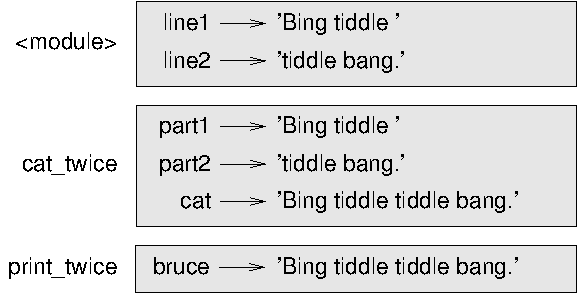
\includegraphics[scale=0.8]{figs/stack.pdf}}
\caption{Διάγραμμα στοίβας.}
\label{fig.stack}
\end{figure}


Τα πλαίσια είναι διατεταγμένα σε μία στοίβα
η οποία υποδεικνύει ποια συνάρτηση κάλεσε ποια και ούτω καθεξής. Σε αυτό το
παράδειγμα, η \verb"print_twice" καλέστηκε από την \verb"cat_twice"
και η \verb"cat_twice" καλέστηκε από την \verb"__main__"
η οποία είναι η συνάρτηση για το ανώτατο πλαίσιο. Όταν δημιουργείτε μία
μεταβλητή έξω από οποιαδήποτε συνάρτηση τότε αυτή ανήκει στην \verb"__main__".


Κάθε παράμετρος αναφέρεται στην τιμή του αντίστοιχου ορίσματός της.
Άρα η {\tt part1} έχει την ίδια τιμή με την {\tt line1}, 
η {\tt part2} έχει την ίδια τιμή με την {\tt line2}  και
η {\tt bruce} έχει την ίδια τιμή με την {\tt cat}.


Αν προκύψει σφάλμα κατά την κλήση μιας συνάρτησης τότε η Python
εμφανίζει το όνομα της συνάρτησης, το όνομα της συνάρτησης που την κάλεσε
και το όνομα της συνάρτησης η οποία κάλεσε αυτήν μέχρις ότου φτάσει στην
\verb"__main__".


Για παράδειγμα, αν προσπαθήσετε να χρησιμοποιήσετε την  {\tt cat} 
μέσα στην \verb"print_twice" τότε θα πάρετε ένα μήνυμα λάθους {\tt NameError}:


\begin{verbatim}
Traceback (innermost last):
  File "test.py", line 13, in __main__
    cat_twice(line1, line2)
  File "test.py", line 5, in cat_twice
    print_twice(cat)
  File "test.py", line 9, in print_twice
    print cat
NameError: name 'cat' is not defined
\end{verbatim}
%

Αυτή η λίστα συναρτήσεων ονομάζεται {\bf αναδρομική ανίχνευση} (traceback) και σας πληροφορεί σε ποιο φάκελο του προγράμματος παρουσιάστηκε το λάθος, σε ποια γραμμή και ποιες συναρτήσεις εκτελούνταν εκείνη τη στιγμή. Σας δείχνει επίσης τη γραμμή του κώδικα από την οποία προκλήθηκε το λάθος.
\index{traceback}

Η σειρά των συναρτήσεων στην αναδρομή είναι ίδια με την σειρά των
πλαισίων στο διάγραμμα κατάστασης. Η συνάρτηση η οποία τρέχει αυτή τη στιγμή 
βρίσκεται στο κάτω μέρος.



\section{Γόνιμες και κενές συναρτήσεις}
\index{fruitful function}
\index{void function}
\index{function, fruitful}
\index{function, void}

Κάποιες από τις συναρτήσεις που χρησιμοποιούμε, όπως οι συναρτήσεις
μαθηματικών, επιστρέφουν αποτελέσματα και λόγω έλλειψης κάποιου καλύτερου ονόματος τις αποκαλώ {\bf γόνιμες συναρτήσεις} (fruitful functions). Άλλες συναρτήσεις, όπως η \verb"print_twice", εκτελούν μια ενέργεια αλλά δεν επιστρέφουν κάποια τιμή. Αυτές ονομάζονται {\bf κενές συναρτήσεις} (void functions).

Σχεδόν κάθε φορά που καλείτε μία γόνιμη συνάρτηση θέλετε να χρησιμοποιήσετε
και το αποτέλεσμα της. Για παράδειγμα, ίσως το εκχωρήσετε σε μία μεταβλητή ή το 
χρησιμοποιήσετε ως μέρος μιας έκφρασης: 


\begin{verbatim}
x = math.cos(radians)
golden = (math.sqrt(5) + 1) / 2
\end{verbatim}
%

Όταν καλείτε μια συνάρτηση σε διαδραστική λειτουργία τότε η Python 
εμφανίζει το αποτέλεσμα:


\begin{verbatim}
>>> math.sqrt(5)
2.2360679774997898
\end{verbatim}
%

Αλλά αν καλέσετε μια γόνιμη συνάρτηση σε ένα σενάριο από μόνη της, τότε
η επιστρεφόμενη τιμή θα χαθεί για πάντα!


\begin{verbatim}
math.sqrt(5)
\end{verbatim}
%

Αυτό το σενάριο υπολογίζει την τετραγωνική ρίζα του 5 αλλά από την στιγμή που
δεν αποθηκεύει ή δεν εμφανίζει το αποτέλεσμα, δεν είναι και πολύ χρήσιμο.
\index{interactive mode}
\index{script mode}

Οι κενές (void) συναρτήσεις μπορεί να εμφανίζουν κάτι στην οθόνη ή να έχουν κάποιο αποτέλεσμα αλλά δεν έχουν επιστρεφόμενη τιμή. Αν προσπαθήσετε να εκχωρήσετε το αποτέλεσμα σε μία μεταβλητή τότε θα πάρετε μια ειδική τιμή με όνομα {\tt None}.
\index{None special value}
\index{special value!None}

\begin{verbatim}
>>> result = print_twice('Bing')
Bing
Bing
>>> print result
None
\end{verbatim}
%

Η τιμή {\tt None} δεν είναι ίδια με την συμβολοσειρά \verb"'None'".
Είναι μια ειδική τιμή η οποία έχει τον δικό της τύπο:


\begin{verbatim}
>>> print type(None)
<type 'NoneType'>
\end{verbatim}
%

Όλες οι συναρτήσεις οι οποίες έχουμε γράψει μέχρι στιγμής είναι κενές (void). 
Θα ξεκινήσουμε να γράφουμε γόνιμες (fruitful) συναρτήσεις σε μερικά κεφάλαια.


\section{Γιατί συναρτήσεις}
\index{function, reasons for}

Ίσως να μην είναι σαφής ο λόγος για τον οποίο αξίζει να χωρίζουμε
ένα πρόγραμμα σε συναρτήσεις αλλά υπάρχουν αρκετοί λόγοι:


\begin{itemize}

\item Η δημιουργία μιας νέας συνάρτησης σας δίνει την δυνατότητα να ονοματίσετε 
ένα σύνολο δηλώσεων το οποίο κάνει το πρόγραμμα ευκολότερο στην ανάγνωση
και στην αποσφαλμάτωση.


\item Οι συναρτήσεις μπορούν να κάνουν ένα πρόγραμμα μικρότερο καταργώντας
τον επαναλαμβανόμενο κώδικα. Αν κάνετε κάποια αλλαγή αργότερα τότε θα χρειαστεί
να την κάνετε μόνο σε ένα σημείο.


\item Η διαίρεση ενός μεγάλου προγράμματος σε συναρτήσεις σας επιτρέπει να
αποσφαλματώνετε τα κομμάτια ένα ένα και μετά να τα ενώνετε όλα μαζί 
σε ένα ολόκληρο λειτουργικό πρόγραμμα.


\item Οι καλοσχεδιασμένες συναρτήσεις είναι συχνά χρήσιμες για πολλά προγράμματα. Μόλις γράψετε μία και την αποσφαλματώσετε τότε μπορείτε να την χρησιμοποιήσετε πολλές φορές.


\end{itemize}


\section{Εισαγωγή από μονάδα λογισμικού με from}

Η Python παρέχει δύο τρόπους εισαγωγής μονάδων λογισμικού αλλά 
μέχρι στιγμής έχουμε ήδη δει μόνο αυτόν:


\begin{verbatim}
>>> import math
>>> print math
<module 'math' (built-in)>
>>> print math.pi
3.14159265359
\end{verbatim}
%

Αν εισάγετε την {\tt math} τότε θα πάρετε ένα αντικείμενο μονάδας λογισμικού με όνομα {\tt math} το οποίο περιέχει σταθερές όπως η {\tt pi} 
και συναρτήσεις όπως η {\tt sin} και η {\tt exp}.

Δεν μπορείτε όμως να αποκτήσετε απευθείας πρόσβαση στην {\tt pi}, 
θα πάρετε ένα μήνυμα λάθους:


\begin{verbatim}
>>> print pi
Traceback (most recent call last):
  File "<stdin>", line 1, in <module>
NameError: name 'pi' is not defined
\end{verbatim}
%

Εναλλακτικά, μπορείτε να εισάγετε ένα αντικείμενο από μια μονάδα έτσι:

\begin{verbatim}
>>> from math import pi
\end{verbatim}
%

Τώρα μπορείτε να έχετε απευθείας πρόσβαση στην {\tt pi} χωρίς
τον συμβολισμό τελείας:
\index{dot notation}


\begin{verbatim}
>>> print pi
3.14159265359
\end{verbatim}
%

Ή μπορείτε να χρησιμοποιήσετε τον τελεστή αστεράκι για να τα εισάγετε
όλα από την μονάδα:


\begin{verbatim}
>>> from math import *
>>> cos(pi)
-1.0
\end{verbatim}


Το πλεονέκτημα του να εισάγουμε τα πάντα από τη μαθηματική μονάδα λογισμικού είναι ότι μπορεί ο κώδικάς σας να είναι πιο συνοπτικός. Το μειονέκτημα είναι ότι μπορεί να προκύψουν συγκρούσεις στα ονόματα που έχουν οριστεί στις διάφορες μονάδες ή μεταξύ ενός ονόματος από μία μονάδα και μίας από τις μεταβλητές σας.



\section{Αποσφαλμάτωση}
\label{editor}
\index{debugging}

Ίσως αντιμετωπίσετε προβλήματα με τα κενά διαστήματα και τους στηλοθέτες (tabs) αν χρησιμοποιείτε έναν επεξεργαστή κειμένου για να γράψετε τα σενάριά σας.
Ο καλύτερος τρόπος για να αποφύγετε τέτοιου είδους προβλήματα είναι να χρησιμοποιείτε αποκλειστικά κενά διαστήματα (καθόλου στηλοθέτες). Οι περισσότεροι επεξεργαστές κειμένου που γνωρίζουν Python το κάνουν αυτό εξ ορισμού αλλά κάποιοι άλλοι δεν το κάνουν.
\index{whitespace}

Συνήθως οι στηλοθέτες και τα κενά διαστήματα είναι αόρατα, γεγονός που 
δυσκολεύει την αποσφαλμάτωση και γι αυτό  είναι προτιμότερο να βρείτε έναν επεξεργαστή που θα διαχειρίζεται αυτός την ενδοπαραγραφοποίηση για εσάς.

Επίσης, μην ξεχνάτε να αποθηκεύετε το πρόγραμμά σας προτού το τρέξετε.
Κάποια περιβάλλοντα ανάπτυξης το κάνουν αυτόματα αλλά κάποια άλλα όχι.
Σε αυτήν την περίπτωση, το πρόγραμμα που κοιτάτε στον επεξεργαστή κειμένου δεν είναι το ίδιο με το πρόγραμμα που τρέχετε.

Η αποσφαλμάτωση μπορεί να είναι χρονοβόρα αν τρέχετε συνεχώς το ίδιο 
εσφαλμένο πρόγραμμα ξανά και ξανά!

Σιγουρευτείτε πως ο κώδικας που κοιτάτε είναι ο κώδικας που τρέχετε.
Αν δεν είστε σίγουροι, γράψτε μία \verb"print 'hello'" 
στην αρχή του προγράμματός σας και τρέξτε το ξανά. Αν δεν δείτε  
\verb"hello" τότε σημαίνει ότι δεν τρέχετε το σωστό πρόγραμμα!



\section{Ορολογία}

\begin{description}

\item[συνάρτηση:] Μία ακολουθία δηλώσεων με συγκεκριμένη ονομασία η οποία εκτελεί κάποιες
χρήσιμες λειτουργίες. Οι συναρτήσεις μπορεί να παίρνουν ορίσματα αλλά μπορεί και όχι.
Επίσης μπορεί να παράγουν κάποιο αποτέλεσμα αλλά μπορεί και όχι.
\index{function}

\item[ορισμός συνάρτησης:] Είναι μία δήλωση η οποία δημιουργεί μια νέα συνάρτηση 
προσδιορίζοντας το όνομα της, τις παραμέτρους και τις δηλώσεις που εκτελεί.
\index{function definition}

\item[αντικείμενο συνάρτησης:] Μία τιμή η οποία δημιουργείται από έναν ορισμό συνάρτησης.
Το όνομα της συνάρτησης είναι μία μεταβλητή η οποία αναφέρεται σε ένα αντικείμενο
συνάρτησης.
\index{function definition}

\item[επικεφαλίδα:] Η πρώτη γραμμή του ορισμού μιας συνάρτησης.
\index{header}

\item[σώμα:] Η ακολουθία δηλώσεων μέσα σε έναν ορισμό συνάρτησης.
\index{body}

\item[παράμετρος:] Μία μεταβλητή που χρησιμοποιείται μέσα σε μία συνάρτηση και 
στην οποία αποδίδεται η τιμή που περνιέται σαν όρισμα.
\index{parameter}

\item[κλήση συνάρτησης:] Μία δήλωση η οποία εκτελεί μια συνάρτηση. Αποτελείται από το
όνομα της συνάρτησης ακολουθούμενο από μία λίστα ορισμάτων.
\index{function call}

\item[όρισμα:] Μία τιμή η οποία παρέχεται σε μια συνάρτηση όταν αυτή καλείται.
Αυτή η τιμή εκχωρείται στην αντίστοιχη παράμετρο στη συνάρτηση.
\index{argument}

\item[τοπική μεταβλητή:] Μία μεταβλητή ορισμένη μέσα σε μια συνάρτηση, η οποία 
μπορεί να χρησιμοποιηθεί (έχει εμβέλεια) μόνο μέσα στη συνάρτησή της.
\index{local variable}

\item[επιστρεφόμενη τιμή:] Το αποτέλεσμα μιας συνάρτησης. Αν μια κλήση συνάρτησης
χρησιμοποιηθεί σαν έκφραση, η επιστρεφόμενη τιμή είναι η τιμή της έκφρασης.
\index{return value}

\item[γόνιμη συνάρτηση:] Μία συνάρτηση η οποία επιστρέφει μια τιμή.
\index{fruitful function}

\item[κενή  (void)  συνάρτηση:] Μία συνάρτηση η οποία δεν επιστρέφει κάποια τιμή.
\index{void function}

\item[μονάδα λογισμικού ή άρθρωμα (module):] Ένα αρχείο το οποίο περιέχει μία συλλογή συναφών συναρτήσεων και άλλους ορισμούς.
\index{module}

\item[δήλωση εισαγωγής (import):] Μία δήλωση η οποία διαβάζει μια μονάδα λογισμικού και δημιουργεί ένα αντικείμενο της μονάδας.
\index{import statement}
\index{statement!import}

\item[αντικείμενο μονάδας λογισμικού:] Μία τιμή που δημιουργείται από την δήλωση {\tt import} και παρέχει πρόσβαση στις τιμές που ορίζονται μέσα σε μία μονάδα λογισμικού.
\index{module}

\item[συμβολισμός με τελεία:] Η σύνταξη για την κλήση μιας συνάρτησης από μια μονάδα λογισμικού καθορίζοντας το όνομα της μονάδας ακολουθούμενο από μία τελεία και στη συνέχεια το όνομα της συνάρτησης.
\index{dot notation}

\item[σύνθεση:] Η χρήση μιας έκφρασης ως μέρος μιας μεγαλύτερης έκφρασης
ή μιας δήλωσης ως μέρος μιας μεγαλύτερης δήλωσης.
\index{composition}

\item[ροή εκτέλεσης:] Η σειρά με την οποία εκτελούνται οι δηλώσεις κατά την εκτέλεση του προγράμματος.
\index{flow of execution}

\item[διάγραμμα στοίβας:] Μία γραφική αναπαράσταση μιας στοίβας από συναρτήσεις, των μεταβλητών τους και των τιμών στις οποίες αναφέρονται.
\index{stack diagram}

\item[πλαίσιο:] Ένα κουτί σε ένα διάγραμμα στοίβας το οποίο αναπαριστά μια κλήση συνάρτησης.
Περιέχει τις τοπικές μεταβλητές και τις παραμέτρους της συνάρτησης.
\index{function frame}
\index{frame}

\item[αναδρομική ανίχνευση:] Μία λίστα των συναρτήσεων που εκτελούνται και η οποία  τυπώνεται όταν παρουσιαστεί μια εξαίρεση.
\index{traceback}


\end{description}


\section{Ασκήσεις}


\begin{exercise}
\index{len function}
\index{function!len}

Η Python έχει μία ενσωματωμένη συνάρτηση που ονομάζεται {\tt len} και
η οποία επιστρέφει το μήκος μιας συμβολοσειράς. Άρα η επιστρεφόμενη τιμή της  \verb"len('allen')" είναι 5.

Γράψτε μία συνάρτηση με όνομα \verb"right_justify" η οποία θα παίρνει
μία συμβολοσειρά με όνομα {\tt s} σαν παράμετρο και θα εμφανίζει 
την συμβολοσειρά με αρκετά κενά διαστήματα έτσι ώστε το τελευταίο γράμμα της
συμβολοσειράς να είναι στη στήλη 70 της οθόνης.


\begin{verbatim}
>>> right_justify('allen')
                                                                 allen
\end{verbatim}
\end{exercise}

\begin{exercise}
\index{function object}
\index{object!function}

Ένα αντικείμενο συνάρτησης είναι μια τιμή την οποία μπορείτε να εκχωρήσετε
σε μία μεταβλητή ή να την περάσετε σαν όρισμα. Για παράδειγμα, η \verb"do_twice" είναι μία συνάρτηση η οποία παίρνει ένα αντικείμενο συνάρτησης σαν ένα όρισμα και το καλεί δύο φορές:


\begin{verbatim}
def do_twice(f):
    f()
    f()
\end{verbatim}

Αυτό είναι ένα παράδειγμα το οποίο χρησιμοποιεί την \verb"do_twice" για να καλέσει δύο φορές μία συνάρτηση που ονομάζεται \verb"print_spam":


\begin{verbatim}
def print_spam():
    print 'spam'

do_twice(print_spam)
\end{verbatim}

\begin{enumerate}


\item Πληκτρολογήστε αυτό το παράδειγμα σε ένα σενάριο και ελέγξτε το.


\item Τροποποιήστε την \verb"do_twice" έτσι ώστε να δέχεται δύο ορίσματα, ένα
αντικείμενο συνάρτησης και μία τιμή και να καλεί την συνάρτηση δύο φορές, περνώντας την τιμή σαν όρισμα.


\item Γράψτε μία γενικότερη εκδοχή της \verb"print_spam", με όνομα
\verb"print_twice" η οποία θα παίρνει μια συμβολοσειρά σαν παράμετρο και θα την
τυπώνει δύο φορές.


\item Χρησιμοποιήστε την τροποποιημένη εκδοχή της \verb"do_twice" για να καλέσετε την \verb"print_twice" δύο φορές, περνώντας την \verb"'spam'" σαν όρισμα.


\item Προσδιορίστε μία νέα συνάρτηση με όνομα \verb"do_four" η οποία θα 
παίρνει ένα αντικείμενο συνάρτησης και μία τιμή και θα καλεί την συνάρτηση τέσσερις φορές, περνώντας την τιμή σαν παράμετρο. Πρέπει να υπάρχουν μόνο δύο δηλώσεις στο σώμα αυτής της συνάρτησης, όχι τέσσερις.


\end{enumerate}

Λύση:  \url{http://thinkpython.com/code/do_four.py}.
\\
\end{exercise}



\begin{exercise}

Αυτή η άσκηση μπορεί να υλοποιηθεί με τη χρήση δηλώσεων και άλλων
χαρακτηριστικών που έχουμε μάθει μέχρι στιγμής.


\begin{enumerate}

\item Γράψτε μία συνάρτηση η οποία σχεδιάζει ένα πλέγμα όπως το ακόλουθο :
\index{grid}


\begin{verbatim}
+ - - - - + - - - - +
|         |         |
|         |         |
|         |         |
|         |         |
+ - - - - + - - - - +
|         |         |
|         |         |
|         |         |
|         |         |
+ - - - - + - - - - +
\end{verbatim}
%

Σημείωση: Για να εμφανίσετε περισσότερες από μία τιμές σε μία γραμμή μπορείτε να τυπώσετε μία ακολουθία χωρισμένη με κόμματα:


\begin{verbatim}
print '+', '-'
\end{verbatim}
%

Αν η ακολουθία τελειώνει με κόμμα, η Python αφήνει την γραμμή ημιτελή 
έτσι ώστε η επόμενη εμφανιζόμενη τιμή να εμφανιστεί στην ίδια γραμμή.


\begin{verbatim}
print '+',
print '-'
\end{verbatim}
%

Η έξοδος αυτών των δηλώσεων είναι  \verb"'+ -'". 

Μία δήλωση {\tt print} από μόνη της ολοκληρώνει την τρέχουσα γραμμή
και πηγαίνει στην επόμενη γραμμή.

\item Γράψτε μία συνάρτηση η οποία θα σχεδιάζει ένα παρόμοιο πλέγμα
με τέσσερις σειρές και τέσσερις στήλες.


\end{enumerate}

Λύση:  \url{http://thinkpython.com/code/grid.py}. 
Αυτή η άσκηση είναι βασισμένη σε μία άσκηση του  Oualline,
{\em Practical C Programming, Third Edition}, O'Reilly Media, 1997.

\end{exercise}





\chapter{Μελέτη περίπτωσης: σχεδίαση διεπαφής}
\label{turtlechap}

Τα παραδείγματα κώδικα αυτού του κεφαλαίου είναι διαθέσιμα στην διεύθυνση 
\url{http://thinkpython.com/code/polygon.py}.


\section{TurtleWorld}
\label{turtleworld}
\index{TurtleWorld}
\index{Swampy}

Για να συνοδεύσει αυτό το βιβλίο, ο καθηγητής Allen έχει γράψει ένα πακέτο λογισμικού που ονομάζεται Swampy. Μπορείτε να κατεβάσετε το Swampy από τον σύνδεσμο \url{http://thinkpython.com/swampy} και να ακολουθήσετε τις οδηγίες εκεί για να το εγκαταστήσετε στον υπολογιστή σας.

Ένα {\bf πακέτο λογισμικού} (package) είναι μια συλλογή από μονάδες λογισμικού. Μία από τις μονάδες του Swampy είναι η {\tt TurtleWorld}, η οποία παρέχει ένα σύνολο συναρτήσεων για τον σχεδιασμό γραμμών κατευθύνοντας χελώνες στην οθόνη.
\index{package}

Αν το Swampy έχει εγκατασταθεί σαν ένα πακέτο λογισμικού στον υπολογιστή σας, 
τότε μπορείτε να εισάγετε την {\tt TurtleWorld} με τον εξής τρόπο:


\begin{verbatim}
from swampy.TurtleWorld import *
\end{verbatim}


Αν κατεβάσατε τις μονάδες του Swampy αλλά δεν τις εγκαταστήσατε σαν πακέτο, τότε μπορείτε είτε να δουλέψετε στον κατάλογο ο οποίος περιέχει τα αρχεία του Swampy είτε να προσθέσετε αυτόν τον κατάλογο στην διαδρομή αναζήτησης της  Python. Τώρα μπορείτε να εισάγετε την {\tt TurtleWorld} έτσι:


\begin{verbatim}
from TurtleWorld import *
\end{verbatim}


Οι λεπτομέρειες της διαδικασίας εγκατάστασης και της προσθήκης της διαδρομής
αναζήτησης στην  Python  εξαρτώνται από το σύστημά σας. Γι' αυτό το λόγο, αντί να συμπεριλάβω αυτές τις λεπτομέρειες εδώ, θα προσπαθήσω να διατηρήσω τις τρέχουσες πληροφορίες για διάφορα συστήματα στην διεύθυνση: \url{http://thinkpython.com/swampy}.

Δημιουργήστε ένα αρχείο με όνομα {\tt mypolygon.py} και γράψτε 
τον ακόλουθο κώδικα:

\begin{verbatim}
from swampy.TurtleWorld import *

world = TurtleWorld()
bob = Turtle()
print bob

wait_for_user()
\end{verbatim}
%

Η πρώτη γραμμή εισάγει ό,τι υπάρχει στην μονάδα {\tt TurtleWorld} 
του πακέτου {\tt swampy}. 
\index{import statement}
\index{statement!import}

Οι επόμενες γραμμές δημιουργούν την TurtleWorld η οποία εκχωρείται στην
{\tt world} και μία  Turtle  η οποία εκχωρείται στην {\tt bob}. 
Τυπώνοντας την {\tt bob} παράγεται κάτι τέτοιο:


\begin{verbatim}
<TurtleWorld.Turtle instance at 0xb7bfbf4c>
\end{verbatim}
%

Αυτό σημαίνει ότι η {\tt bob} αναφέρεται σε ένα {\bf στιγμιότυπο} (instance) της Turtle όπως αυτή ορίζεται στην μονάδα λογισμικού {\tt TurtleWorld}. Σε αυτό το πλαίσιο, το "στιγμιότυπο" είναι ένα τμήμα ενός συνόλου. Αυτή η Turtle είναι μία από το σύνολο των εφικτών Turtles.
\index{instance}

H \verb"wait_for_user" λέει στην TurtleWorld 
να περιμένει από τον χρήστη να κάνει κάτι, παρόλο που σε αυτήν
τη περίπτωση δεν υπάρχουν και πολλά που μπορεί να κάνει ο χρήστης
εκτός από το να κλείσει το παράθυρο.

Η TurtleWorld παρέχει αρκετές συναρτήσεις "χελωνο-οδήγησης": 
την {\tt fd} και την {\tt bk} για μπροστά και πίσω,
την {\tt lt} και την {\tt rt} για στροφή στα αριστερά και στα δεξιά.
Επίσης, η κάθε χελώνα κρατάει ένα στυλό ο οποίος βρίσκεται είτε κάτω είτε πάνω.
Αν το στυλό βρίσκεται κάτω τότε η χελώνα αφήνει μια γραμμή όταν κινείται. Οι συναρτήσεις {\tt pu} και {\tt pd} αντιπροσωπεύουν τα "pen up" και "pen down".


Προσθέστε αυτές τις γραμμές στο πρόγραμμα (αφού δημιουργήσετε την {\tt bob} και προτού καλέσετε την \verb"wait_for_user") για να σχεδιάσετε μια ορθή γωνία:

\begin{verbatim}
fd(bob, 100)
lt(bob)
fd(bob, 100)
\end{verbatim}
%

Η πρώτη γραμμή λέει στην {\tt bob} να κάνει 100 βήματα μπροστά.
Η δεύτερη γραμμή της λέει να στρίψει αριστερά.

Όταν τρέξετε αυτό το πρόγραμμα, θα πρέπει να δείτε την {\tt bob} να
μετακινείται ανατολικά και μετά βόρεια, αφήνοντας δύο ευθύγραμμα τμήματα από πίσω.

Τροποποιήστε το πρόγραμμα για να σχεδιάσετε ένα τετράγωνο. Μη προχωρήσετε μέχρι
να δείτε ότι δουλεύει.

%\newpage

\section{Απλή επανάληψη}
\label{repetition}
\index{repetition}


Κατά πάσα πιθανότητα γράψατε κάτι τέτοιο (χωρίς τον κώδικα ο οποίος δημιουργεί
την TurtleWorld και περιμένει τον χρήστη):

\begin{verbatim}
fd(bob, 100)
lt(bob)

fd(bob, 100)
lt(bob)

fd(bob, 100)
lt(bob)

fd(bob, 100)
\end{verbatim}
%

Μπορούμε να κάνουμε το ίδιο πράγμα πιο συνοπτικά με μία δήλωση  {\tt for}. 
Προσθέστε αυτό το παράδειγμα στην  {\tt mypolygon.py}  και τρέξτε το ξανά:
\index{for loop}
\index{loop!for}
\index{statement!for}


\begin{verbatim}
for i in range(4):
    print 'Hello!'
\end{verbatim}
%

Θα πρέπει να δείτε κάτι τέτοιο:


\begin{verbatim}
Hello!
Hello!
Hello!
Hello!
\end{verbatim}
%

Αυτή είναι η πιο απλή χρήση της δήλωσης {\tt for}. Αργότερα θα δούμε περισσότερες χρήσεις της αλλά αυτό είναι αρκετό ώστε να μπορείτε να ξαναγράψετε το πρόγραμμα σχεδιασμού τετραγώνων. Μην προχωρήσετε μέχρι να το κάνετε.

Αυτή είναι μια δήλωση {\tt for} η οποία σχεδιάζει ένα τετράγωνο:

\begin{verbatim}
for i in range(4):
    fd(bob, 100)
    lt(bob)
\end{verbatim}
%

Η σύνταξη μίας δήλωσης  {\tt for}  είναι παρόμοια με τον ορισμό μιας
συνάρτησης. Έχει μία επικεφαλίδα που τελειώνει με μία άνω και κάτω τελεία και ένα σώμα εμφωλευμένο. Το σώμα μπορεί να έχει οποιοδήποτε πλήθος δηλώσεων.
\index{loop}

Μία δήλωση {\tt for} ονομάζεται και {\bf βρόχος} (loop) επειδή
η ροή εκτέλεσης περνά μέσα από το σώμα και στη συνέχεια επιστρέφει βροχοειδώς 
πίσω στην κορυφή. Στην συγκεκριμένη περίπτωση το σώμα εκτελείται τέσσερις φορές.

Στην πραγματικότητα, αυτή η έκδοση είναι λίγο διαφορετική από τον προηγούμενο
κώδικα σχεδίασης τετραγώνων δεδομένου ότι κάνει μία ακόμη στροφή αφότου σχεδιάσει και την τελευταία πλευρά του τετραγώνου. Η επιπλέον στροφή παίρνει λίγο περισσότερο χρόνο αλλά απλοποιεί τον κώδικα αφού  κάνουμε το ίδιο πράγμα κάθε φορά μέσα στο βρόχο. Αυτή η έκδοση έχει επίσης ως αποτέλεσμα να αφήνει τη χελώνα στην αρχική θέση, με φορά προς την αρχική κατεύθυνση.


\section{Ασκήσεις}

Ακολουθεί μία σειρά ασκήσεων οι οποίες χρησιμοποιούν τη TurtleWorld και στόχος τους είναι η διασκέδαση, αλλά παράλληλα έχουν κάποια σημασία. Προσπαθήστε να βρείτε τη σημασία τους καθώς δουλεύετε πάνω σε αυτές.

Οι παρακάτω ενότητες έχουν λύσεις για αυτές τις ασκήσεις, γι αυτό μην τις κοιτάξετε μέχρι να τις λύσετε (ή τουλάχιστον να προσπαθήστε).

\begin{enumerate}

\item Γράψτε μία συνάρτηση με όνομα {\tt square} που θα παίρνει μια παράμετρο με όνομα {\tt t}, η οποία θα είναι μία χελώνα (turtle). Θα πρέπει να χρησιμοποιεί τη χελώνα για να σχεδιάσει
ένα τετράγωνο.

Γράψτε μία κλήση συνάρτησης η οποία θα περνάει την {\tt bob} 
σαν όρισμα στην {\tt square} και μετά ξανατρέξτε το πρόγραμμα.

\item Προσθέστε μία ακόμα παράμετρο στη {\tt square} με όνομα {\tt length}. 
Στη συνέχεια τροποποιήστε το σώμα ώστε η {\tt length} να είναι το μήκος των πλευρών και μετά τροποποιήστε την κλήση της συνάρτησης δίνοντας ένα ακόμα όρισμα. Τρέξτε το πρόγραμμα ξανά και ελέγξτε το για διάφορες τιμές της {\tt length}. 

\item Οι συναρτήσεις {\tt lt} και {\tt rt} κάνουν στροφές 90 μοιρών
από προεπιλογή, αλλά μπορείτε να δώσετε ένα δεύτερο όρισμα που θα
καθορίζει τον αριθμό των μοιρών. Για παράδειγμα, η {\tt lt(bob, 45)} περιστρέφει την bob 45 μοίρες στα αριστερά.

Κάντε ένα αντίγραφο της {\tt square} και αλλάξτε το όνομά της σε 
{\tt polygon}. Προσθέστε μία παράμετρο με όνομα {\tt n} και
τροποποιήστε το σώμα ώστε να σχεδιάζει ένα κανονικό πολύγωνο n πλευρών.
Σημείωση: Οι εξωτερικές γωνίες ενός κανονικού πολυγώνου n πλευρών είναι
$360/n$ μοίρες.
\index{polygon function}
\index{function!polygon}

\item Γράψτε μία συνάρτηση με όνομα {\tt circle}  η οποία θα παίρνει μία χελώνα {\tt t} 
και μία ακτίνα {\tt r} ως παραμέτρους και θα σχεδιάζει έναν κατά προσέγγιση κύκλο επικαλούμενη τη 
{\tt polygon} με ένα κατάλληλο μήκος και αριθμό πλευρών. Ελέγξτε τη συνάρτησή σας με ένα εύρος τιμών της 
{\tt r}.
\index{circle function}
\index{function!circle}

Σημείωση 1η: Υπολογίστε την περίμετρο του κύκλου και σιγουρευτείτε πως {\tt length * n = circumference}.

Σημείωση 2η: Αν η {\tt bob} είναι πολύ αργή, μπορείτε να την επιταχύνετε αλλάζοντας
την {\tt bob.delay} η οποία είναι ο χρόνος μεταξύ των κινήσεων σε δευτερόλεπτα. Με {\tt bob.delay = 0.01}  θα πρέπει να κινείται γρηγορότερα.

% Αλλάξτε το σε  world.delay
% change this to world.delay

\item Φτιάξτε μία πιο γενική έκδοση της {\tt circle} με όνομα {\tt arc} 
η οποία θα παίρνει μία επιπλέον παράμετρο με όνομα {\tt angle} και η οποία θα καθορίζει ποιο τμήμα του  κύκλου θα σχεδιαστεί. Η {\tt angle} μετριέται σε μοίρες και έτσι όταν {\tt angle=360} η {\tt arc}
θα πρέπει να σχεδιάσει ένα πλήρες κύκλο.
\index{ function}
\index{function!arc}

\end{enumerate}

\section{Ενθυλάκωση}

Η πρώτη άσκηση σας ζητάει να βάλετε τον κώδικα σχεδίασης τετραγώνου σε
έναν ορισμό συνάρτησης και μετά να καλέσετε τη συνάρτηση περνώντας τη χελώνα σαν παράμετρο. Αυτή είναι μία λύση:


\begin{verbatim}
def square(t):
    for i in range(4):
        fd(t, 100)
        lt(t)

square(bob)
\end{verbatim}
%

Οι ενδότερες δηλώσεις {\tt fd} και {\tt lt} είναι διπλά εμφωλευμένες για να
δείξουν ότι βρίσκονται εντός του βρόχου {\tt for}, ο οποίος βρίσκεται μέσα στον
ορισμό της συνάρτησης. Η επόμενη γραμμή,  {\tt square(bob)},  βρίσκεται στο
ίδιο επίπεδο με το αριστερό όριο ώστε να είναι και στο τέλος του βρόχου {\tt for} αλλά και του ορισμού της συνάρτησης.

Μέσα στη συνάρτηση, η {\tt t} αναφέρεται στην ίδια χελώνα που αναφέρεται και η
{\tt bob}. Άρα η {\tt lt(t)} έχει το ίδιο αποτέλεσμα με τη {\tt lt(bob)}. 
Οπότε γιατί να μην καλέσουμε την παράμετρο {\tt bob};  Η γενική ιδέα είναι ότι η {\tt t} μπορεί να είναι οποιαδήποτε χελώνα (όχι μόνο η {\tt bob}) και έτσι μπορείτε να δημιουργήσετε μία δεύτερη χελώνα και να την περάσετε ως όρισμα στη {\tt square}:


\begin{verbatim}
ray = Turtle()
square(ray)
\end{verbatim}
%

Το να συμπεριλάβετε ένα κομμάτι του κώδικα μέσα σε μία συνάρτηση ονομάζεται {\bf ενθυλάκωση} (encapsulation). Ένα από τα πλεονεκτήματα της ενθυλάκωσης είναι ότι προσδίδει ένα όνομα στον κώδικα το οποίο χρησιμεύει ως είδος τεκμηρίωσης. Ένα άλλο πλεονέκτημα είναι πως αν θέλετε να χρησιμοποιήσετε ξανά τον κώδικα τότε είναι πιο λακωνικό να καλέσετε δύο φορές μία συνάρτηση παρά να αντιγράφετε ολόκληρο το σώμα της!
\index{encapsulation}


\section{Γενίκευση}

Το επόμενο βήμα είναι να προσθέσουμε μία παράμετρο  {\tt length}  στην  {\tt square}. Λύση:


\begin{verbatim}
def square(t, length):
    for i in range(4):
        fd(t, length)
        lt(t)

square(bob, 100)
\end{verbatim}
%

Η προσθήκη μίας παραμέτρου σε μία συνάρτηση ονομάζεται {\bf γενίκευση} (generalization) διότι κάνει την συνάρτηση πιο γενική:  στην προηγούμενη έκδοση το τετράγωνο είχε πάντα το ίδιο μέγεθος, ενώ σε αυτήν την έκδοση μπορεί να έχει οποιοδήποτε μέγεθος.
\index{generalization}

Το επόμενο βήμα είναι επίσης μία γενίκευση. Αντί η {\tt polygon} να σχεδιάζει τετράγωνα, σχεδιάζει κανονικά πολύγωνα με οποιονδήποτε αριθμό πλευρών. Λύση:


\begin{verbatim}
def polygon(t, n, length):
    angle = 360.0 / n
    for i in range(n):
        fd(t, length)
        lt(t, angle)

polygon(bob, 7, 70)
\end{verbatim}
%

Αυτός ο κώδικας σχεδιάζει ένα πολύγωνο 7 πλευρών με μήκος πλευράς 70. Αν έχετε περισσότερα από μερικά αριθμητικά ορίσματα τότε μπορεί να ξεχάσετε τι είναι τι ή σε ποια σειρά θα πρέπει να βρίσκονται. Είναι έγκυρο, και κάποιες φορές χρήσιμο να χρησιμοποιείτε τα ονόματα των παραμέτρων στη λίστα ορισμάτων:

\begin{verbatim}
polygon(bob, n=7, length=70)
\end{verbatim}
%

Αυτά ονομάζονται {\bf λέξεις-κλειδιά ορίσματα} (keyword arguments) επειδή περιέχουν τα ονόματα των παραμέτρων σαν "λέξεις-κλειδιά" (δεν θα πρέπει να συγχέονται με τις λέξεις κλειδιά της Python όπως η {\tt while} και η {\tt def}).
\index{keyword argument}
\index{argument!keyword}

Αυτή η σύνταξη κάνει το πρόγραμμα πιο ευανάγνωστο. Είναι επίσης μία υπενθύμιση σχετικά με το πως λειτουργούν τα ορίσματα και οι παράμετροι: όταν καλείτε μία συνάρτηση τα ορίσματα εκχωρούνται στις παραμέτρους.


\section{Σχεδίαση διεπαφής}

Το επόμενο βήμα είναι να γράψετε τη {\tt circle} η οποία παίρνει μία ακτίνα {\tt r} ως παράμετρο. Μία απλή λύση η οποία χρησιμοποιεί την {\tt polygon} για να σχεδιάσει ένα πολύγωνο 50 πλευρών είναι:


\begin{verbatim}
def circle(t, r):
    circumference = 2 * math.pi * r
    n = 50
    length = circumference / n
    polygon(t, n, length)
\end{verbatim}
%

Η πρώτη γραμμή υπολογίζει την περίμετρο ενός κύκλου με ακτίνα {\tt r} 
χρησιμοποιώντας τον τύπο  $2 \pi r$. Από τη στιγμή που χρησιμοποιούμε τη 
{\tt math.pi} θα πρέπει να εισάγουμε τη {\tt math}. Κατά συνθήκη, οι δηλώσεις
{\tt import} μπαίνουν συνήθως στην αρχή του σεναρίου.

Η {\tt n} είναι το πλήθος των ευθύγραμμων τμημάτων στον κατά προσέγγιση κύκλο μας και η {\tt length} είναι το μήκος κάθε τμήματος. Επομένως, η {\tt polygon} 
σχεδιάζει ένα πολύγωνο 50 πλευρών το οποίο προσεγγίζει ένα κύκλο με ακτίνα  {\tt r}. 

Ένας από τους περιορισμούς αυτής της λύσης είναι ότι η  {\tt n}  είναι μία σταθερά, το οποίο σημαίνει ότι για πολύ μεγάλους κύκλους τα ευθύγραμμα τμήματα είναι πολύ μεγάλα και για μικρούς κύκλους σπαταλάμε χρόνο σχεδιάζοντας πολύ μικρά τμήματα. Μία λύση θα ήταν να γενικεύαμε τη συνάρτηση περνώντας την {\tt n} σαν παράμετρο. Αυτό θα δώσει στο χρήστη περισσότερο έλεγχο (όταν καλεί την {\tt circle}) αλλά η διεπαφή θα γίνει λίγο πιο πολύπλοκη.
\index{interface}

Η {\bf διεπαφή} (interface) μίας συνάρτησης είναι μία σύνοψη του πως αυτή χρησιμοποιείται: ποιες είναι οι παράμετροι; τι κάνει η συνάρτηση; ποια είναι η επιστρεφόμενη τιμή; Μία διεπαφή είναι "ξεκάθαρη" εάν είναι "όσο το δυνατόν πιο απλή αλλά όχι απλούστερη. (Αϊνστάιν)"
\index{Einstein, Albert}

Σε αυτό το παράδειγμα, η {\tt r} ανήκει στη διεπαφή επειδή προσδιορίζει τον κύκλο που θα σχεδιαστεί. Η {\tt n} δεν είναι τόσο κατάλληλη επειδή αναφέρεται στις λεπτομέρειες του πως ο κύκλος θα πρέπει να υλοποιηθεί.

Αντί να υπερφορτώσουμε την διεπαφή, είναι καλύτερα να διαλέξουμε μία κατάλληλη
τιμή για την {\tt n} ανάλογα με την περιφέρεια :

\begin{verbatim}
def circle(t, r):
    circumference = 2 * math.pi * r
    n = int(circumference / 3) + 1
    length = circumference / n
    polygon(t, n, length)
\end{verbatim}
%

Τώρα, ο αριθμός των τμημάτων είναι (περίπου) {\tt circumference/3}, 
έτσι το μήκος κάθε τμήματος είναι (περίπου) 3, το οποίο είναι αρκετά μικρό ώστε
ο κύκλος να φαίνεται καλός αλλά και αρκετά μεγάλο για να είναι αποδοτικό και κατάλληλο για οποιοδήποτε μέγεθος κύκλου.


\section{Ανακατασκευή κώδικα}
\label{refactoring}
\index{refactoring}

Όταν έγραψα τη {\tt circle}, είχα την δυνατότητα να χρησιμοποιήσω την {\tt polygon} επειδή ένα πολύπλευρο πολύγωνο είναι μία καλή προσέγγιση ενός κύκλου. Αλλά η {\tt arc} δεν είναι τόσο συνεργάσιμη. Δεν μπορούμε να χρησιμοποιήσουμε τη {\tt polygon} ή τη {\tt circle} για να σχεδιάσουμε ένα τόξο.

Μία εναλλακτική λύση είναι να ξεκινήσουμε με ένα αντίγραφο της {\tt polygon} και να το μετατρέψουμε σε {\tt arc}. Το αποτέλεσμα θα μπορούσε να είναι κάπως έτσι:

\begin{verbatim}
def arc(t, r, angle):
    arc_length = 2 * math.pi * r * angle / 360
    n = int(arc_length / 3) + 1
    step_length = arc_length / n
    step_angle = float(angle) / n

    for i in range(n):
        fd(t, step_length)
        lt(t, step_angle)
\end{verbatim}
%

Το δεύτερο μισό αυτής της συνάρτησης μοιάζει με τη {\tt polygon} αλλά
δεν μπορούμε να επαναχρησιμοποιήσουμε τη {\tt polygon} χωρίς να αλλάξουμε τη
διεπαφή. Θα μπορούσαμε να γενικεύσουμε τη {\tt polygon} έτσι ώστε να παίρνει μία γωνία σαν τρίτο όρισμα αλλά τότε το {\tt polygon} δεν θα είναι πλέον ένα κατάλληλο όνομα! Αντ'αυτού, ας καλέσουμε την πιο γενική συνάρτηση  {\tt polyline}:

\begin{verbatim}
def polyline(t, n, length, angle):
    for i in range(n):
        fd(t, length)
        lt(t, angle)
\end{verbatim}
%

Τώρα μπορούμε να ξαναγράψουμε την {\tt polygon} και την {\tt arc} χρησιμοποιώντας την {\tt polyline}:

\begin{verbatim}
def polygon(t, n, length):
    angle = 360.0 / n
    polyline(t, n, length, angle)

def arc(t, r, angle):
    arc_length = 2 * math.pi * r * angle / 360
    n = int(arc_length / 3) + 1
    step_length = arc_length / n
    step_angle = float(angle) / n
    polyline(t, n, step_length, step_angle)
\end{verbatim}
%

Τέλος, μπορούμε να ξαναγράψουμε τη {\tt circle} χρησιμοποιώντας και πάλι την {\tt arc}:

\begin{verbatim}
def circle(t, r):
    arc(t, r, 360)
\end{verbatim}
%

Αυτή η διαδικασία αναδιάταξης ενός προγράμματος για τη βελτίωση των διεπαφών των συναρτήσεων και τη διευκόλυνση της επαναχρησιμοποίησης του κώδικα ονομάζεται {\bf ανακατασκευή κώδικα} (refactoring). Σε αυτήν την περίπτωση, παρατηρήσαμε ότι υπήρχε παρόμοιος κώδικας στη {\tt arc} και στη 
{\tt polygon} και έτσι τον "ανακατασκευάσαμε" στην {\tt polyline}.
\index{refactoring}


Εάν το είχαμε προβλέψει, ίσως είχαμε γράψει τη {\tt polyline} εξαρχής και έτσι θα αποφεύγαμε την ανακατασκευή. Πολλές φορές όμως δεν γνωρίζετε αρκετά στην αρχή ενός έργου (project) για να σχεδιάσετε όλες τις διεπαφές. Μερικές φορές η ανακατασκευή είναι ένα σημάδι ότι έχετε μάθει κάτι.


\section{Πλάνο ανάπτυξης}
\index{development plan!encapsulation and generalization}

Ένα {\bf πλάνο ανάπτυξης} (development plan) είναι μία διαδικασία για την συγγραφή προγραμμάτων. Η μέθοδος που χρησιμοποιήσαμε σε αυτήν την περίπτωση είναι η "ενθυλάκωση" και η  "γενίκευση". Τα βήματα αυτής της μεθόδου είναι:

\begin{enumerate}

\item Ξεκινήστε γράφοντας ένα μικρό πρόγραμμα χωρίς ορισμούς συναρτήσεων.

\item Από τη στιγμή που το πρόγραμμά σας δουλεύει, ενθυλακώστε το σε μία
συνάρτηση και δώστε του ένα όνομα.

\item Γενικεύστε τη συνάρτηση προσθέτοντας κατάλληλες παραμέτρους.

\item Επαναλάβετε τα βήματα 1-3 μέχρις ότου να έχετε ένα σύνολο από λειτουργικές συναρτήσεις. Αντιγράψτε τον λειτουργικό κώδικα για να αποφύγετε την επαναπληκτρολόγηση (και την επαναποσφαλμάτωση).

\item Ψάξτε για δυνατότητες βελτίωσης του προγράμματος μέσω της ανακατασκευής κώδικα. Για παράδειγμα, εάν έχετε παρόμοιο κώδικα σε μερικά σημεία, σκεφτείτε να τον ανακατασκευάσετε σε μία καταλληλότερη γενική συνάρτηση.

\end{enumerate}

Αυτή η διαδικασία έχει κάποια μειονεκτήματα (θα δούμε εναλλακτικές λύσεις αργότερα) αλλά μπορεί να είναι χρήσιμη εάν δεν γνωρίζετε εκ των προτέρων πως να σπάσετε το πρόγραμμα σε συναρτήσεις. Αυτή η προσέγγιση σας επιτρέπει να σχεδιάζετε όσο προχωράτε.


\section{Συμβολοσειρά τεκμηρίωσης}
\label{docstring}
\index{docstring}

Μία {\bf συμβολοσειρά τεκμηρίωσης} (docstring) είναι μία συμβολοσειρά στην αρχή μιας συνάρτησης η οποία εξηγεί τη διεπαφή (το ``doc'' είναι συντομογραφία του ``documentation''). Για παράδειγμα:


\begin{verbatim}
def polyline(t, n, length, angle):
    """Draws n line segments with the given length and
    angle (in degrees) between them.  t is a turtle.
    """
    for i in range(n):
        fd(t, length)
        lt(t, angle)
\end{verbatim}
%

Αυτή η συμβολοσειρά τεκμηρίωσης είναι μια συμβολοσειρά με τριπλά εισαγωγικά,
γνωστή και ως πολλυγραμμική (multiline) συμβολοσειρά επειδή τα τριπλά εισαγωγικά επιτρέπουν στη συμβολοσειρά να εκτείνεται σε περισσότερες από μία γραμμές.
\index{quotation mark}
\index{triple-quoted string}
\index{string!triple-quoted}
\index{multiline string}
\index{string!multiline}

Είναι λιτή αλλά περιέχει τις απαραίτητες πληροφορίες που χρειάζεται κάποιος για να χρησιμοποιήσει αυτή τη συνάρτηση. Εξηγεί συνοπτικά τι κάνει η συνάρτηση (χωρίς να υπεισέρχεται σε λεπτομέρειες για το πως το κάνει). Εξηγεί τι επίδραση έχει κάθε παράμετρος στη συμπεριφορά της συνάρτησης και τι τύπο θα πρέπει να έχει η κάθε παράμετρος (αν δεν είναι προφανές).

Η σύνταξη αυτού του είδους τεκμηρίωσης είναι ένα σημαντικό κομμάτι του σχεδιασμού διεπαφής. Μία καλοσχεδιασμένη διεπαφή θα πρέπει να είναι απλό να εξηγηθεί. Αν δυσκολεύεστε να εξηγήσετε κάποια από τις συναρτήσεις σας τότε αυτό είναι ένα σημάδι ότι η διεπαφή θα μπορούσε να βελτιωθεί.



\section{Αποσφαλμάτωση}
\index{debugging}
\index{interface}

Μία διεπαφή είναι σαν μία σύμβαση μεταξύ μίας συνάρτησης και του καλούντος.
Ο καλών συμφωνεί να παρέχει συγκεκριμένες παραμέτρους και η συνάρτηση δέχεται να κάνει μία συγκεκριμένη δουλειά.

Για παράδειγμα, η {\tt polyline} απαιτεί τέσσερα ορίσματα: η {\tt t} θα πρέπει
να είναι μία χελώνα, η {\tt n} είναι ο αριθμός των ευθύγραμμων τμημάτων (θα πρέπει να είναι ακέραιος), η {\tt length} θα πρέπει να είναι ένας θετικός αριθμός και η {\tt angle} θα πρέπει να είναι αριθμός (εννοείται σε μοίρες).

Οι απαιτήσεις αυτές ονομάζονται {\bf προϋποθέσεις} (preconditions) επειδή πρέπει να είναι αληθείς προτού αρχίσει να εκτελείται η συνάρτηση. Αντιστρόφως, οι συνθήκες στο τέλος της συνάρτησης ονομάζονται {\bf μετά-συνθήκες} (post-conditions). Οι μετά-συνθήκες περιλαμβάνουν το προβλεπόμενο αποτέλεσμα της συνάρτησης (όπως τη σχεδίαση ευθύγραμμων τμημάτων) και οποιεσδήποτε άλλες παράπλευρες ενέργειες (όπως η κίνηση της χελώνας ή άλλες αλλαγές στον κόσμο).
\index{precondition}
\index{postcondition}

Οι προϋποθέσεις είναι ευθύνη του καλούντος. Αν ο καλών παραβιάσει μία
(σωστά τεκμηριωμένη) προϋπόθεση και η συνάρτηση δε λειτουργεί σωστά,
τότε το λάθος είναι του καλούντος και όχι της συνάρτησης.

% Removing this because we haven't seen conditionals yet!
%However, for purposes of debugging it is often a good idea for
%functions to check their preconditions rather than assume they are
%true.  If every function checks its preconditions before starting,
%then if something goes wrong, you will know which function to blame.


\section{Ορολογία}

\begin{description}

\item[στιγμιότυπο:] Ένα μέρος ενός συνόλου. Η TurtleWorld σε αυτό το κεφάλαιο
είναι ένα μέρος του συνόλου TurtleWorlds.
\index{instance}


\item[βρόχος:] Ένα κομμάτι του προγράμματος που μπορεί να εκτελείται επανειλημμένα.
\index{loop}

\item[ενθυλάκωση:] Η διαδικασία μετασχηματισμού μίας ακολουθίας δηλώσεων σε έναν ορισμό συνάρτησης.
\index{encapsulation}

\item[γενίκευση:] Η διαδικασία αντικατάστασης κάτι συγκεκριμένου 
(όπως ένας αριθμός) με κάτι πιο γενικευμένου (όπως μία μεταβλητή ή παράμετρος).
\index{generalization}

\item[λέξη-κλειδί όρισμα:] Ένα όρισμα το οποίο περιέχει το όνομα της παραμέτρου ως ''λέξη-κλειδί''.
\index{keyword argument}
\index{argument!keyword}

\item[διεπαφή:] Μία περιγραφή του πώς χρησιμοποιείται μία συνάρτηση, συμπεριλαμβανομένου του
ονόματος και της περιγραφής των ορισμάτων και της επιστρεφόμενης τιμής.
\index{interface}

\item[ανακατασκευή κώδικα:] Η διαδικασία τροποποίησης ενός λειτουργικού προγράμματος για την βελτίωση των 
διεπαφών των συναρτήσεων και άλλων χαρακτηριστικών του κώδικα.
\index{refactoring}

\item[πλάνο ανάπτυξης:] Μία μέθοδος γραφής προγραμμάτων.
\index{development plan}

\item[συμβολοσειρά τεκμηρίωσης:] Μία συμβολοσειρά η οποία εμφανίζεται σε ένα ορισμό συνάρτησης
για να τεκμηριώσει τη διεπαφή της συνάρτησης.
\index{docstring}

\item[προϋπόθεση:] Μία συνθήκη που πρέπει να ικανοποιείται από τον καλούντα προτού ξεκινήσει η συνάρτηση.
\index{precondition}

\item[μετά-συνθήκη:] Μία συνθήκη η οποία πρέπει να ικανοποιηθεί από τη συνάρτηση προτού
τελειώσει.
\index{precondition}

\end{description}


\section{Ασκήσεις}

\begin{exercise}

Κατεβάστε τον κώδικα αυτού του κεφαλαίου από το σύνδεσμο \url{http://thinkpython.com/code/polygon.py}.


\begin{enumerate}

\item Γράψτε κατάλληλες συμβολοσειρές κειμένου για τις {\tt polygon}, {\tt arc} και {\tt circle}. 
\index{stack diagram}

\item Σχεδιάστε ένα διάγραμμα στοίβας το οποίο θα δείχνει την κατάσταση του προγράμματος ενώ εκτελείται η  {\tt circle(bob, radius)}. 
Μπορείτε να κάνετε τις πράξεις με το χέρι ή να προσθέσετε δηλώσεις {\tt print} στον κώδικα.

\item Η έκδοση της  {\tt arc}  στην ενότητα~\ref{refactoring}  δεν είναι πολύ ακριβής επειδή
η γραμμική προσέγγιση του κύκλου δεν είναι ποτέ ένας αληθινός κύκλος. Σαν αποτέλεσμα, η χελώνα τελειώνει
λίγο πιο μακριά από τον σωστό προορισμό. Η δική μου λύση δείχνει έναν τρόπο να περιορίσουμε το φαινόμενο
αυτού του λάθους. Διαβάστε τον κώδικα και δείτε αν μπορείτε να βγάλετε κάποιο νόημα. Εάν σχεδιάσετε ένα
διάγραμμα, ίσως καταλάβετε πως δουλεύει.
\\
\end{enumerate}

\end{exercise}

\begin{figure}
\centerline
{
\includegraphics[scale=0.8]{figs/flowers.pdf}}
\caption{Turtle flowers.}
\label{fig.flowers}
\end{figure}


\begin{exercise}
\index{flower}

Γράψτε ένα σύνολο κατάλληλων γενικών συναρτήσεων οι οποίες θα μπορούν να σχεδιάσουν
λουλούδια όπως αυτά στο Σχήμα~\ref{fig.flowers}.

Λύση: \url{http://thinkpython.com/code/flower.py}. 
Θα χρειαστείτε και την \url{http://thinkpython.com/code/polygon.py}.
\\
\end{exercise}

\begin{figure}
\centerline
{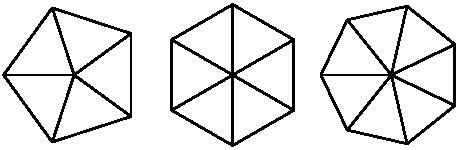
\includegraphics[scale=0.8]{figs/pies.pdf}}
\caption{Turtle pies.}
\label{fig.pies}
\end{figure}


\begin{exercise}
\index{pie}

Γράψτε ένα σύνολο κατάλληλων γενικών συναρτήσεων οι οποίες θα μπορούν να σχεδιάσουν σχήματα όπως στην Εικόνα~\ref{fig.pies}.

Λύση : \url{http://thinkpython.com/code/pie.py}.
\\
\end{exercise}

\begin{exercise}
\index{alphabet}
\index{turtle typewriter}
\index{typewriter, turtle}

Τα γράμματα του αγγλικού αλφαβήτου μπορούν να σχεδιαστούν από ένα σύνολο βασικών στοιχείων,
όπως κάθετες και οριζόντιες γραμμές και μερικές καμπύλες. Σχεδιάστε μία γραμματοσειρά η οποία θα 
μπορεί να υλοποιηθεί με ένα μικρό αριθμό βασικών στοιχείων και στη συνέχεια γράψτε συναρτήσεις
η οποίες θα σχεδιάζουν γράμματα του αγγλικού αλφαβήτου.

Πρέπει να γράψετε μία συνάρτηση για κάθε γράμμα, με ονόματα  \verb"draw_a", \verb"draw_b",  κτλ.,
και να βάλτε της συναρτήσεις σε ένα αρχείο με όνομα {\tt letters.py}.  Μπορείτε να κατεβάσετε μία
''χελώνα δακτυλογράφο'' από εδώ  : \url{http://thinkpython.com/code/typewriter.py}  για να σας
βοηθήσει να ελέγξετε τον κώδικά σας.

Λύση : \url{http://thinkpython.com/code/letters.py}. Θα χρειαστείτε και την :
\url{http://thinkpython.com/code/polygon.py}.
\\
\end{exercise}


\begin{exercise}

Διαβάστε σχετικά με τις σπείρες στο  \url{http://en.wikipedia.org/wiki/Spiral},  και στη συνέχεια γράψτε ένα πρόγραμμα που θα σχεδιάζει μία Αρχιμήδεια σπείρα (ή κάποιο από τα υπόλοιπα είδη). Λύση: \url{http://thinkpython.com/code spiral.py}.
\index{spiral}
\index{Archimedian spiral}

\end{exercise}


\chapter{Δηλώσεις υπό συνθήκη και αναδρομή}

\section{Τελεστής υπολογισμού υπολοίπου ακέραιας διαίρεσης}
\index{modulus operator}
\index{operator!modulus}

Ο {\bf τελεστής υπόλοιπο} (modulus operator) εφαρμόζεται σε ακέραιους αριθμούς και επιστρέφει το υπόλοιπο όταν ο πρώτος τελεστέος διαιρείται από το δεύτερο. Στην Python, ο τελεστής  "υπόλοιπο" είναι το σύμβολο επί τοις εκατό (\verb"%").  Η σύνταξη είναι η ίδια όπως και με τους άλλους τελεστές:

\begin{verbatim}
>>> quotient = 7 / 3
>>> print quotient
2
>>> remainder = 7 % 3
>>> print remainder
1
\end{verbatim}
%

Έτσι το 7 διαιρούμενο με το 3 μας δίνει υπόλοιπο 1.

Ο τελεστής "υπόλοιπο" μπορεί να αποδειχτεί ιδιαίτερα χρήσιμος. Για παράδειγμα, μπορείτε να ελέγξετε αν ένας αριθμός {\tt x} διαιρείται από έναν άλλο αριθμό {\tt y} αν η έκφραση {\tt x \% y} δίνει αποτέλεσμα μηδέν.
\index{divisibility}


Επίσης, μπορείτε να εξάγετε το δεξιότερο ψηφίο ή ψηφία από έναν αριθμό. Για παράδειγμα, η έκφραση {\tt x \% 10} δίνει το τελευταίο ψηφίο του {\tt x} (μονάδες στη βάση του 10) και η {\tt x \% 100} δίνει τα δύο
τελευταία ψηφία.


\section{Λογικές εκφράσεις}
\index{boolean expression}
\index{expression!boolean}
\index{logical operator}
\index{operator!logical}

Μία {\bf λογική έκφραση} (boolean expression) είναι μία έκφραση η οποία είναι είτε αληθής είτε ψευδής. Τα ακόλουθα παραδείγματα χρησιμοποιούν τον τελεστή {\tt ==}, ο οποίος συγκρίνει δύο τελεστέους και παράγει  {\tt True} αν είναι ίσοι ή {\tt False} αλλιώς:

\begin{verbatim}
>>> 5 == 5
True
>>> 5 == 6
False
\end{verbatim}
%

Η  {\tt True}  και η  {\tt False}  είναι ειδικές τιμές οι οποίες ανήκουν στον τύπο {\tt bool},  δεν είναι συμβολοσειρές:
\index{True special value}
\index{False special value}
\index{special value!True}
\index{special value!False}
\index{bool type}
\index{type!bool}

\begin{verbatim}
>>> type(True)
<type 'bool'>
>>> type(False)
<type 'bool'>
\end{verbatim}
%

Ο τελεστής {\tt ==} είναι ένας από τους {\bf σχεσιακούς τελεστές} (relational operators):

\begin{verbatim}
      x != y               # x is not equal to y
      x > y                # x is greater than y
      x < y                # x is less than y
      x >= y               # x is greater than or equal to y
      x <= y               # x is less than or equal to y
\end{verbatim}
%

Πιθανώς να γνωρίζετε αυτές τις πράξεις αλλά τα σύμβολα της Python
είναι διαφορετικά από τα σύμβολα των μαθηματικών. Ένα συνηθισμένο λάθος είναι η χρήση ενός μονό συμβόλου ισότητας ({\tt =}) αντί για διπλό σύμβολο ισότητας ({\tt ==}). Να θυμάστε ότι το {\tt =} είναι ένας τελεστής εκχώρησης και το {\tt ==} είναι ένας σχεσιακός τελεστής. Δεν υπάρχει κάτι αντίστοιχο των {\tt =<} και {\tt =>}.
\index{relational operator}
\index{operator!relational}


\section{Λογικοί τελεστές}
\index{logical operator}
\index{operator!logical}

Υπάρχουν τρεις {\bf λογικοί τελεστές} (logical operators): ο {\tt and}, ο {\tt or} και ο {\tt not}. Η σημασιολογική ερμηνεία αυτών των τελεστών είναι παρόμοια με το νόημά τους στα Αγγλικά. Για παράδειγμα, η {\tt x > 0 and x < 10} είναι αληθής μόνο αν το {\tt x} είναι μεγαλύτερο του μηδενός και μικρότερο του 10.
\index{and operator}
\index{or operator}
\index{not operator}
\index{operator!and}
\index{operator!or}
\index{operator!not}

Η {\tt n\%2 == 0 or n\%3 == 0} είναι αληθείς αν οποιαδήποτε από τις δύο συνθήκες είναι αληθής. Αν δηλαδή ο αριθμός διαιρείται ή με το 2 ή με το 3.

Τέλος ο τελεστής {\tt not} ακυρώνει μια λογική έκφραση. Άρα η {\tt not (x > y)} είναι αληθής αν η {\tt x > y} είναι ψευδής και αυτό συμβαίνει αν το {\tt x} είναι μικρότερο ή ίσο του {\tt y}.

Αν θέλαμε να είμαστε αυστηροί, οι τελεστέοι των λογικών τελεστών θα έπρεπε να είναι λογικές εκφράσεις αλλά η  Python δεν είναι τόσο αυστηρή. Κάθε μη μηδενικός αριθμός διερμηνεύεται ως "αληθής" (''true'').

\begin{verbatim}
>>> 17 and True
True
\end{verbatim}
%

Αυτή η ευελιξία μπορεί να είναι χρήσιμη αλλά υπάρχουν κάποιες μικρές λεπτομέρειες οι οποίες  μπορεί να προκαλέσουν σύγχυση και καλύτερα να το αποφύγετε (εκτός αν ξέρετε τι κάνετε).


\section{Εκτέλεση υπό συνθήκη}
\label{conditional.execution}

\index{conditional statement}
\index{statement!conditional}
\index{if statement}
\index{statement!if}
\index{conditional execution}

Προκειμένου να γράψουμε χρήσιμα προγράμματα πρέπει να μπορούμε
να ελέγχουμε συνθήκες και να αλλάζουμε αναλόγως τη συμπεριφορά του προγράμματος. Αυτή τη δυνατότητα μας την δίνουν οι {\bf δηλώσεις υπό συνθήκη} (conditional statements) και η  απλούστερη από αυτές είναι η δήλωση {\tt if}:

\begin{verbatim}
if x > 0:
    print 'x is positive'
\end{verbatim}
%

Η λογική έκφραση μετά την {\tt if} ονομάζεται {\bf συνθήκη} (condition). Αν είναι αληθής τότε η εμφωλευμένη δήλωση αρχίζει να εκτελείται ενώ αν είναι ψευδής δεν γίνεται τίποτα.
\index{condition}
\index{compound statement}
\index{statement!compound}

Οι δηλώσεις  {\tt if}  έχουν την ίδια δομή με τους ορισμούς συνάρτησης:
μία επικεφαλίδα ακολουθούμενη από ένα εμφωλευμένο σώμα. Δηλώσεις όπως αυτές
ονομάζονται {\bf σύνθετες δηλώσεις} (compound statements).

Δεν υπάρχει όριο στο πλήθος των δηλώσεων που μπορούμε να βάλουμε μέσα στο σώμα
αλλά πρέπει να υπάρχει τουλάχιστον μία. Ενίοτε όμως είναι χρήσιμο να έχουμε ένα σώμα χωρίς δηλώσεις (σαν κρατημένο χώρο για τον κώδικα που δεν έχουμε γράψει ακόμη). Σε αυτή τη περίπτωση μπορούμε να χρησιμοποιήσουμε τη δήλωση {\tt pass} η οποία δεν κάνει τίποτα.
\index{pass statement}
\index{statement!pass}

\begin{verbatim}
if x < 0:
    pass          # need to handle negative values!
\end{verbatim}
%

\section{Εναλλακτική εκτέλεση}
\label{alternative.execution}
\index{alternative execution}
\index{else keyword}
\index{keyword!else}

Μία δεύτερη μορφή της δήλωσης {\tt if} είναι η {\bf εναλλακτική εκτέλεση} (alternative execution), στην οποία υπάρχουν δύο ενδεχόμενα και το ποιο από τα δύο θα εκτελεστεί καθορίζεται από την συνθήκη. Η σύνταξη είναι κάπως έτσι:

\begin{verbatim}
if x%2 == 0:
    print 'x is even'
else:
    print 'x is odd'
\end{verbatim}
%

Αν το υπόλοιπο της διαίρεσης του {\tt x} με το 2 είναι 0 τότε αντιλαμβανόμαστε ότι το {\tt x} είναι άρτιος και το πρόγραμμα εμφανίζει ένα μήνυμα γι αυτό το αποτέλεσμα. Αν η συνθήκη είναι ψευδής τότε εκτελείται το δεύτερο σύνολο δηλώσεων. Από τη στιγμή που η συνθήκη είναι είτε αληθής είτε ψευδής τότε μπορεί να εκτελεστεί μόνο μία από τις εναλλακτικές. Οι εναλλακτικές ονομάζονται {\bf κλάδοι} (branches) επειδή στην ουσία "διακλαδώνουν" τη ροή εκτέλεσης.
\index{branch}



\section{Αλυσιδωτές συνθήκες}
\index{chained conditional}
\index{conditional!chained}

Μερικές φορές χρειαζόμαστε περισσότερους από δύο κλάδους γιατί υπάρχουν περισσότερες από δύο πιθανότητες. Ένας τρόπος για να εκφράσουμε έναν τέτοιο υπολογισμό είναι μία {\bf αλυσιδωτή συνθήκη} (chained conditional):

\begin{verbatim}
if x < y:
    print 'x is less than y'
elif x > y:
    print 'x is greater than y'
else:
    print 'x and y are equal'
\end{verbatim}
%

Η {\tt elif} είναι συντομογραφία της ``else if''. Δεν υπάρχει όριο στον αριθμό των δηλώσεων {\tt elif} αλλά όπως και πριν θα εκτελεστεί μόνο ένας από τους κλάδους. Αν υπάρχει μία δήλωση {\tt else} τότε θα πρέπει να βρίσκεται στο τέλος αλλά δεν είναι υποχρεωτικό να υπάρχει.
\index{elif keyword}
\index{keyword!elif}


\begin{verbatim}
if choice == 'a':
    draw_a()
elif choice == 'b':
    draw_b()
elif choice == 'c':
    draw_c()
\end{verbatim}
%

Η κάθε συνθήκη ελέγχεται με τη σειρά. Αν η πρώτη είναι λάθος τότε ελέγχεται η δεύτερη και ούτω καθεξής. Αν μία από αυτές είναι αληθής τότε εκτελείται ο αντίστοιχος κλάδος και η δήλωση τερματίζει. Ακόμη κι αν περισσότερες από μία συνθήκες είναι αληθείς μόνο ο πρώτος αληθής κλάδος εκτελείται.


\section{Εμφωλευμένες συνθήκες}
\index{nested conditional}
\index{conditional!nested}

Ένας όρος μπορεί να είναι εμφωλευμένος μέσα σε έναν άλλο. Επομένως, θα μπορούσαμε να είχαμε γράψει το παράδειγμα της τριχοτόμησης κάπως έτσι:

\begin{verbatim}
if x == y:
    print 'x and y are equal'
else:
    if x < y:
        print 'x is less than y'
    else:
        print 'x is greater than y'
\end{verbatim}
%

Η εξωτερική συνθήκη περιέχει δύο κλάδους. Ο πρώτος κλάδος περιέχει μία απλή δήλωση και ο δεύτερος περιέχει μία άλλη δήλωση {\tt if} η οποία έχει δύο κλάδους από μόνη της. Αυτοί οι δύο κλάδοι είναι απλές δηλώσεις παρόλο που θα μπορούσαν επίσης να είναι δηλώσεις υπό συνθήκη.

Παρόλο που η ενδοπαραγραφοποίηση των δηλώσεων κάνει προφανή τη δομή, οι εμφωλευμένες συνθήκες δεν είναι εύκολο να διαβαστούν γρήγορα. Γενικά είναι προτιμότερο να τις αποφεύγετε αν μπορείτε.

Οι λογικοί τελεστές παρέχουν συχνά ένα τρόπο για την απλοποίηση των εμφωλευμένων δηλώσεων υπό συνθήκη. Για παράδειγμα, μπορούμε να γράψουμε ξανά τον ακόλουθο κώδικα χρησιμοποιώντας μία απλή υπόθεση:

\begin{verbatim}
if 0 < x:
    if x < 10:
        print 'x is a positive single-digit number.'
\end{verbatim}
%

Η δήλωση {\tt print} εκτελείται μόνο αν είναι αληθείς και οι δυο συνθήκες,
έτσι μπορούμε να έχουμε το ίδιο αποτέλεσμα με τον τελεστή {\tt and}:

\begin{verbatim}
if 0 < x and x < 10:
    print 'x is a positive single-digit number.'
\end{verbatim}


\section{Αναδρομή}
\label{recursion}
\index{recursion}


Μία συνάρτηση μπορεί να καλέσει μία άλλη συνάρτηση αλλά μπορεί επίσης να καλέσει και τον ίδιο της τον εαυτό. Η χρησιμότητα αυτού του χαρακτηριστικού μπορεί να μην είναι προφανής, αλλά αποδεικνύεται ένα από τα πιο μαγικά πράγματα που μπορεί να κάνει ένα πρόγραμμα. Για παράδειγμα δείτε την ακόλουθη συνάρτηση:

\begin{verbatim}
def countdown(n):
    if n <= 0:
        print 'Blastoff!'
    else:
        print n
        countdown(n-1)
\end{verbatim}
%

Αν η παράμετρος {\tt n} είναι 0 ή αρνητική τότε στην έξοδο θα έχουμε τη λέξη ``Blastoff!''. Αλλιώς θα τυπώσει την τιμή της {\tt n} και στη συνέχεια θα καλέσει τον εαυτό της με όρισμα {\tt n-1}.

Τι συμβαίνει αν καλέσουμε αυτή τη συνάρτηση έτσι:

\begin{verbatim}
>>> countdown(3)
\end{verbatim}
%

Η εκτέλεση της {\tt countdown} ξεκινάει με {\tt n=3}  και από τη στιγμή
που η {\tt n} είναι μεγαλύτερη του 0 τυπώνει την τιμή 3 και έπειτα καλεί τον εαυτό της...

\begin{quote}
Η εκτέλεση της {\tt countdown} ξεκινάει με {\tt n=2} και από τη στιγμή που η
{\tt n} είναι μεγαλύτερη του 0 τυπώνει την τιμή 2 και έπειτα καλεί τον εαυτό της...

\begin{quote}
Η εκτέλεση της {\tt countdown} ξεκινάει με {\tt n=1} και από τη στιγμή που η
{\tt n} είναι μεγαλύτερη του 0 τυπώνει την τιμή 1 και έπειτα καλεί τον εαυτό της...

\begin{quote}
Η εκτέλεση της {\tt countdown} ξεκινάει με {\tt n=0} και από τη στιγμή που η
{\tt n} δεν είναι μεγαλύτερη του 0 τυπώνει τη λέξη ``Blastoff!'' και έπειτα επιστρέφει.
\end{quote}

Η {\tt countdown} με {\tt n=1} επιστρέφει.
\end{quote}

Η {\tt countdown} με {\tt n=2} επιστρέφει.
\end{quote}

Η {\tt countdown} με {\tt n=3} επιστρέφει.

Και στη συνέχεια βρίσκεστε πίσω στη \verb"__main__".  Έτσι η συνολική έξοδος
είναι κάπως έτσι:

\begin{verbatim}
3
2
1
Blastoff!
\end{verbatim}
%

Μία συνάρτηση η οποία καλεί τον εαυτό της ονομάζεται {\bf αναδρομική} (recursive) και η διαδικασία ονομάζεται {\bf αναδρομή} (recursion).
\index{recursion}
\index{function!recursive}

Ένα ακόμα παράδειγμα είναι μία συνάρτηση η οποία εμφανίζει μία συμβολοσειρά 
{\tt n} φορές:


\begin{verbatim}
def print_n(s, n):
    if n <= 0:
        return
    print s
    print_n(s, n-1)
\end{verbatim}
%

Αν {\tt n <= 0} η δήλωση {\tt return} τερματίζει τη συνάρτηση και η ροή εκτέλεσης επιστρέφει αμέσως στην συνάρτηση που την κάλεσε ενώ οι υπόλοιπες γραμμές της συνάρτησης δεν εκτελούνται.
\index{return statement}
\index{statement!return}

Η υπόλοιπη συνάρτηση είναι παρόμοια με τη {\tt countdown}: 
εάν η {\tt n} είναι μεγαλύτερη του 0 τότε εμφανίζει την {\tt s} και καλεί τον
εαυτό της για να εμφανίσει την {\tt s} $n-1$ επιπλέον φορές. Έτσι ο αριθμός γραμμών της εξόδου είναι {\tt 1 + (n - 1)}, δηλαδή ίσο με {\tt n}.

Για απλά παραδείγματα όπως αυτά, ίσως είναι ευκολότερο να χρησιμοποιήσετε ένα βρόχο {\tt for}. Αλλά αργότερα θα δούμε παραδείγματα τα οποία είναι δύσκολο να γραφτούν με {\tt for} και ευκολότερο να γραφτούν με αναδρομή. Γι αυτό το λόγο είναι καλό να ξεκινήσετε νωρίς.



\section{Διαγράμματα στοίβας για αναδρομικές συναρτήσεις}
\label{recursive.stack}
\index{stack diagram}
\index{function frame}
\index{frame}

Στην παράγραφο ~\ref{stackdiagram} χρησιμοποιήσαμε ένα διάγραμμα στοίβας για να
αναπαραστήσουμε την κατάσταση του προγράμματος κατά τη διάρκεια μιας κλήσης συνάρτησης. Το ίδιο είδος διαγράμματος μπορεί να βοηθήσει για να ερμηνεύσουμε μια αναδρομική συνάρτηση.

Κάθε φορά που καλείται μία συνάρτηση, η Python δημιουργεί ένα καινούργιο πλαίσιο συνάρτησης το οποίο περιέχει τις τοπικές μεταβλητές και τις παραμέτρους της συνάρτησης. Για μία αναδρομική συνάρτηση μπορεί να υπάρχουν περισσότερα από ένα πλαίσια στη στοίβα ταυτόχρονα.

Το σχήμα~\ref{fig.stack2} δείχνει ένα διάγραμμα στοίβας της {\tt countdown} η οποία έχει καλεστεί με {\tt n = 3}.

\begin{figure}
\centerline
{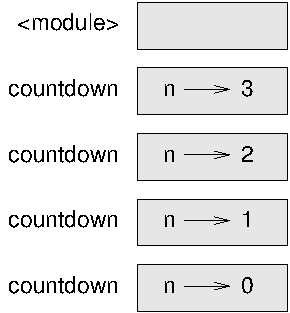
\includegraphics[scale=0.8]{figs/stack2.pdf}}
\caption{Διάγραμμα στοίβας.}
\label{fig.stack2}
\end{figure}


Ως συνήθως, στη κορυφή της στοίβας είναι το πλαίσιο για τη \verb"__main__". Είναι άδειο γιατί δε δημιουργήσαμε ούτε μεταβλητές στη \verb"__main__", ούτε της περάσαμε κάποιο όρισμα.
\index{base case}
\index{recursion!base case}

Τα τέσσερα πλαίσια {\tt countdown} έχουν διαφορετικές τιμές για την παράμετρο {\tt n}. Το κάτω μέρος της στοίβας όπου {\tt n=0} ονομάζεται {\bf περίπτωση βάσης} (base case). Δεν υπάρχουν άλλα πλαίσια γιατί δεν γίνεται άλλη αναδρομική κλήση.\\

\begin{exercise}

Σχεδιάστε ένα διάγραμμα στοίβας για τη \verb"print_n" η οποία θα καλείται με \verb"s = 'Hello'" και {\tt n=2}.

\end{exercise}

\begin{exercise}

Γράψτε μία συνάρτηση με όνομα \verb"do_n" η οποία θα παίρνει ένα αντικείμενο συνάρτησης και έναν αριθμό {\tt n} σαν ορίσματα και θα καλεί τη δοθείσα συνάρτηση {\tt n} φορές.

\end{exercise}


\section{Άπειρη αναδρομή}
\index{infinite recursion}
\index{recursion!infinite}
\index{runtime error}
\index{error!runtime}
\index{traceback}

Αν μία αναδρομή δε φτάνει ποτέ σε μία περίπτωση βάσης, τότε συνεχίζει κάνοντας αναδρομικές κλήσεις για πάντα και το πρόγραμμα δεν τερματίζει ποτέ. Αυτή είναι γνωστή ως {\bf άπειρη αναδρομή} (infinite recursion) και γενικά δεν είναι καλή ιδέα. Αυτό είναι ένα πολύ μικρό πρόγραμμα με άπειρη αναδρομή:

\begin{verbatim}
def recurse():
    recurse()
\end{verbatim}
%

Στα περισσότερα προγραμματιστικά περιβάλλοντα, ένα πρόγραμμα με άπειρη αναδρομή δεν τρέχει για πάντα. Η Python αναφέρει ένα μήνυμα λάθους όταν φτάσει στο μέγιστο βάθος αναδρομής:
\index{exception!RuntimeError}
\index{RuntimeError}

\begin{verbatim}
  File "<stdin>", line 2, in recurse
  File "<stdin>", line 2, in recurse
  File "<stdin>", line 2, in recurse
                  .
                  .
                  .
  File "<stdin>", line 2, in recurse
RuntimeError: Maximum recursion depth exceeded
\end{verbatim}
%

Αυτή η αναδρομική ανίχνευση είναι λίγο μεγαλύτερη από αυτή που είδαμε στο προηγούμενο κεφάλαιο. Όταν συμβεί αυτό το λάθος θα υπάρχουν 1000 αναδρομικά πλαίσια στη στοίβα!


\section{Είσοδος από το πληκτρολόγιο}
\index{keyboard input}

Τα προγράμματα που έχουμε γράψει μέχρι στιγμής είναι λίγο αγενή με την έννοια ότι δε δέχονται καμία είσοδο από το χρήστη, κάνουν απλά το ίδιο πράγμα κάθε φορά.

Η Python 2 παρέχει μία ενσωματωμένη συνάρτηση με όνομα \verb"raw_input" η οποία δέχεται είσοδο από το πληκτρολόγιο, ενώ στην Python 3 αυτή η συνάρτηση ονομάζεται {\tt input}. Όταν καλείται αυτή η συνάρτηση, το πρόγραμμα σταματάει και περιμένει το χρήστη να πληκτρολογήσει κάτι. Όταν ο χρήστης πατήσει {\sf Return} ή {\sf Enter}, το πρόγραμμα συνεχίζει και η  \verb"raw_input" επιστρέφει ότι πληκτρολόγησε ο χρήστης σαν μία συμβολοσειρά.
\index{Python 3}
\index{raw\_input function}
\index{function!raw\_input}

\begin{verbatim}
>>> text = raw_input()
What are you waiting for?
>>> print text
What are you waiting for?
\end{verbatim}
%

Πριν το πρόγραμμα πάρει την είσοδο από το χρήστη, καλό θα ήταν να εμφανίσει ένα μήνυμα προτροπής το οποίο θα λέει στο χρήστη τι να εισάγει. Η \verb"raw_input" μπορεί να πάρει σαν όρισμα ένα τέτοιο μήνυμα:
\index{prompt}

\begin{verbatim}
>>> name = raw_input('What...is your name?\n')
What...is your name?
Arthur, King of the Britons!
>>> print name
Arthur, King of the Britons!
\end{verbatim}
%

Το \verb"\n" στο τέλος του μηνύματος αναπαριστά μία {\bf newline},
η οποία είναι ένας ειδικός χαρακτήρας που προκαλεί αλλαγή γραμμής.
Για αυτό η είσοδος του χρήστη εμφανίζεται κάτω από το μήνυμα προτροπής.
\index{newline}

Εάν περιμένετε ο χρήστης να πληκτρολογήσει έναν ακέραιο, τότε μπορείτε να δοκιμάσετε να μετατρέψετε την επιστρεφόμενη τιμή σε {\tt int}:

\begin{verbatim}
>>> prompt = 'What...is the airspeed velocity of an unladen swallow?\n'
>>> speed = raw_input(prompt)
What...is the airspeed velocity of an unladen swallow?
17
>>> int(speed)
17
\end{verbatim}
%

Αλλά αν ο χρήστης πληκτρολογήσει κάτι διαφορετικό από μία σειρά ψηφίων τότε θα
πάρετε ένα μήνυμα λάθους:

\begin{verbatim}
>>> speed = raw_input(prompt)
What...is the airspeed velocity of an unladen swallow?
What do you mean, an African or a European swallow?
>>> int(speed)
ValueError: invalid literal for int()
\end{verbatim}
%

Θα δούμε πώς χειριζόμαστε τέτοιου είδους λάθη αργότερα.
\index{ValueError}
\index{exception!ValueError}


\section{Αποσφαλμάτωση}
\label{whitespace}
\index{debugging}
\index{traceback}

Η Python εμφανίζει αναδρομικά πολλές πληροφορίες όταν συμβεί κάποιο λάθος,
κάτι το οποίο μπορεί να είναι υπερβολικό και ειδικά όταν υπάρχουν πολλά πλαίσια στη στοίβα. Συνήθως, τα πιο χρήσιμα σημεία είναι:

\begin{itemize}

\item Τι είδος λάθους ήταν, και 

\item Πότε συνέβη.

\end{itemize}

Τα συντακτικά λάθη είναι συνήθως εύκολο να βρεθούν αλλά υπάρχουν και μερικές
παγίδες. Τα λάθη λευκού κενού διαστήματος (whitespace errors) μπορεί να είναι
δυσεπίλυτα γιατί τα κενά διαστήματα (spaces) και οι στηλοθέτες (tabs) 
είναι αόρατα και συνηθίζουμε να τα αγνοούμε. 
\index{whitespace}

\begin{verbatim}
>>> x = 5
>>>  y = 6
  File "<stdin>", line 1
    y = 6
    ^
SyntaxError: invalid syntax
\end{verbatim}
%

Σε αυτό το παράδειγμα το πρόβλημα είναι ότι η δεύτερη γραμμή έχει
εσοχή ενός κενού διαστήματος αλλά το μήνυμα λάθους δείχνει το {\tt y}, 	
το οποίο είναι παραπλανητικό. Σε γενικές γραμμές τα μηνύματα λάθους υποδεικνύουν που ανέκυψε το πρόβλημα αλλά το πραγματικό λάθος μπορεί να είναι νωρίτερα στον κώδικα, ακόμη και σε προηγούμενη γραμμή.
\index{error!runtime}
\index{runtime error}

Το ίδιο ισχύει και για τα λάθη χρόνου εκτέλεσης.

Υποθέστε ότι προσπαθείτε να υπολογίσετε ένα σηματοθορυβικό λόγο σε ντεσιμπέλ (dB). Ο τύπος είναι $SNR_{db} = 10 \log_{10} (P_{signal} / P_{noise})$ και ίσως το γράφατε κάπως έτσι:

\begin{verbatim}
import math
signal_power = 9
noise_power = 10
ratio = signal_power / noise_power
decibels = 10 * math.log10(ratio)
print decibels
\end{verbatim}
%

Αλλά όταν το τρέχετε στην  Python 2 παίρνετε ένα μήνυμα λάθους: 
\index{exception!OverflowError}
\index{OverflowError}

\begin{verbatim}
Traceback (most recent call last):
  File "snr.py", line 5, in ?
    decibels = 10 * math.log10(ratio)
OverflowError: math range error
\end{verbatim}
%

Το μήνυμα λάθους υποδεικνύει την γραμμή 5 αλλά δεν υπάρχει
κάτι λάθος σε αυτήν τη γραμμή. Για να βρούμε το πραγματικό λάθος
ίσως θα ήταν χρήσιμο να εμφανίζαμε την τιμή της {\tt ratio},
η οποία αποδεικνύεται ότι είναι 0. Το πρόβλημα είναι στη γραμμή 4
επειδή όταν διαιρούμε δύο ακέραιους αριθμούς έχουμε ακέραια διαίρεση.
Η λύση είναι να αναπαραστήσουμε την ισχύ του σήματος και την ισχύ του
θορύβου με αριθμούς κινητής υποδιαστολής.
\index{floor division}
\index{division!floor}

Γενικά, τα μηνύματα λάθους σας λένε που ανέκυψε το πρόβλημα αλλά
αυτό δεν σημαίνει ότι προκλήθηκε εκεί.

Στην Python 3 αυτό το παράδειγμα δεν προκαλεί σφάλμα γιατί ο τελεστής
της διαίρεσης εκτελεί δεκαδική διαίρεση ακόμα και με ακέραιους τελεστέους.


\section{Ορολογία}

\begin{description}

\item[τελεστής υπολογισμού υπολοίπου ακέραιας διαίρεσης:] Ένας τελεστής 
ο οποίος συμβολίζεται με το σύμβολο επί της εκατό ({\tt \%}). Δουλεύει
με ακεραίους και επιστρέφει το υπόλοιπο όταν διαιρέσουμε δύο αριθμούς.
\index{modulus operator}
\index{operator!modulus}

\item[λογική έκφραση:]  Μία έκφραση της οποίας η τιμή είναι είτε αληθής  ({\tt True}) 
είτε ψευδής  ({\tt False}).
\index{boolean expression}
\index{expression!boolean}

\item[σχεσιακός τελεστής:]  Ένας τελεστής ο οποίος συγκρίνει δύο τελεστέους: 
{\tt ==}, {\tt !=}, {\tt >}, {\tt <}, {\tt >=} και {\tt <=}.

\item[λογικός τελεστής:]  Ένας τελεστής ο οποίος συνδιάζει δύο λογικές εκφράσεις: 
{\tt and}, {\tt or} και {\tt not}.

\item[δηλώσεις υπό συνθήκη:]  Μία δήλωση η οποία ρυθμίζει τη ροή εκτέλεσης με βάση 
κάποια συνθήκη.
\index{conditional statement}
\index{statement!conditional}

\item[συνθήκη:]  Η λογική έκφραση σε μία υπό συνθήκη δήλωση η οποία καθορίζει ποιος
κλάδος θα εκτελεστεί.
\index{condition}

\item[σύνθετη δήλωση:]  Μία δήλωση η οποία αποτελείται από μία επικεφαλίδα και
ένα σώμα. Η επικεφαλίδα τελειώνει με μία άνω και κάτω τελεία  (:) και το σώμα
είναι γραμμένο σε εσοχή σε σχέση με την επικεφαλίδα.
\index{compound statement}

\item[κλάδος:] Μία από τις εναλλακτικές ακολουθίες εντολών σε μία υπό συνθήκη
δήλωση.
\index{branch}

\item[αλυσιδωτές συνθήκες:]  Μία υπό συνθήκη δήλωση με μια σειρά εναλλακτικών
κλάδων.
\index{chained conditional}
\index{conditional!chained}

\item[εμφωλευμένη συνθήκη:]  Μία υπό συνθήκη δήλωση η οποία εμφανίζεται σε
έναν από τους κλάδους μίας άλλης υπό συνθήκης δήλωσης.
\index{nested conditional}
\index{conditional!nested}

\item[αναδρομή:]  Η διαδικασία κατά την οποία καλείται η συνάρτηση η οποία
τρέχει αυτή τη στιγμή.
\index{recursion}

\item[περίπτωση βάσης:]  Ένας υπό συνθήκη κλάδος σε μία αναδρομική συνάρτηση
ο οποίος δεν κάνει καμία αναδρομική κλήση.
\index{base case}

\item[άπειρη αναδρομή:]  Μία αναδρομή η οποία δεν έχει περίπτωση βάσης ή δεν
την φτάνει ποτέ (δηλαδή δεν την επαληθεύει). Και τελικά, μία άπειρη αναδρομή προκαλεί
ένα λάθος χρόνου εκτέλεσης.
\index{infinite recursion}

\end{description}

\section{Ασκήσεις}

\begin{exercise}
\index{Fermat's Last Theorem}

Το τελευταίο θεώρημα του Fermat λέει ότι δεν υπάρχουν θετικοί ακέραιοι $a$, $b$, και $c$ τέτοιοι ώστε

\[ a^n + b^n = c^n \]
%
για οποιαδήποτε τιμή του $n$ μεγαλύτερη του 2.

\begin{enumerate}

\item Γράψτε μία συνάρτηση με όνομα \verb"check_fermat" η οποία
θα παίρνει 4 παραμέτρους, {\tt a}, {\tt b}, {\tt c} και {\tt n}, 
και θα ελέγχει αν ισχύει το θεώρημα του Fermat. Αν το $n$ είναι μεγαλύτερο
του 2 και αποδεικνύεται ότι η σχέση

\[a^n + b^n = c^n \]
%
είναι αληθής, το πρόγραμμα θα πρέπει να εμφανίζει το μήνυμα:
``Holy smokes, Fermat was wrong!''  Αλλιώς θα εμφανίζει:
``No, that doesn't work.''

\item Γράψτε μία συνάρτηση η οποία ζητάει από το χρήστη να εισάγει τιμές
για τις  {\tt a}, {\tt b}, {\tt c} και {\tt n}, τις μετατρέπει
σε ακέραιους και χρησιμοποιεί την \verb"check_fermat" για να ελέγξει αν
παραβιάζουν το θεώρημα του  Fermat.
\\

\end{enumerate}

\end{exercise}


\begin{exercise}
\index{triangle}

Αν σας δοθούν τρία ξυλάκια τότε ίσως μπορέσετε να σχηματίσετε ένα τρίγωνο με αυτά, μπορεί όμως και όχι. Για παράδειγμα, εάν ένα από τα ξυλάκια είναι 12 εκατοστά και τα άλλα δύο είναι 1 εκατοστό το καθένα τότε είναι προφανές ότι δεν θα είστε σε θέση να ενώσετε τα κοντά ξυλάκια μεταξύ τους. Μπορούμε να κάνουμε έναν απλό έλεγχο για οποιοδήποτε συνδυασμό από τρία μήκη για να δούμε αν είναι εφικτό να σχεδιαστεί ένα τρίγωνο:

\begin{quotation}

Εάν ένα από τα τρία μήκη είναι μεγαλύτερο από το άθροισμα των άλλων δύο 
τότε δεν μπορεί να σχηματιστεί τρίγωνο, αλλιώς μπορεί. (Αν το άθροισμα δύο μηκών είναι ίσο με το τρίτο σχηματίζουν ένα "εκφυλισμένο" τρίγωνο.)
\end{quotation}

\begin{enumerate}


\item Γράψτε μία συνάρτηση με όνομα  \verb"is_triangle"  η οποία θα
  παίρνει τρεις ακέραιους σαν ορίσματα και θα εμφανίζει στην έξοδο είτε 
  ``Yes'' είτε ``No'' ανάλογα με το αν μπορείτε ή όχι να σχηματίσετε
  ένα τρίγωνο με τα ξυλάκια των δοθέντων μηκών.

\item Γράψτε μία συνάρτηση η οποία θα ζητάει από το χρήστη να εισάγει τρία
  μήκη για ξυλάκια, θα τα μετατρέπει σε ακέραιους και θα χρησιμοποιεί την 
  \verb"is_triangle"  για να ελέγξει εάν τα ξυλάκια με τα δοθέντα μήκη
  μπορούν να σχεδιάσουν ένα τρίγωνο.\\

\end{enumerate}

\end{exercise}
Οι ακόλουθες ασκήσεις χρησιμοποιούν την  TurtleWorld  από το Κεφάλαιο~\ref{turtlechap}:
\index{TurtleWorld}


\begin{exercise}

Διαβάστε την παρακάτω συνάρτηση και δείτε αν μπορείτε να καταλάβετε τι κάνει.
Στη συνέχεια τρέξτε την και δείτε τα παραδείγματα στο Κεφάλαιο~\ref{turtlechap}.

\begin{verbatim}
def draw(t, length, n):
    if n == 0:
        return
    angle = 50
    fd(t, length*n)
    lt(t, angle)
    draw(t, length, n-1)
    rt(t, 2*angle)
    draw(t, length, n-1)
    lt(t, angle)
    bk(t, length*n)
\end{verbatim}

\end{exercise}


\begin{figure}
\centerline
{
\includegraphics[scale=0.8]{figs/koch.pdf}}
\caption{A Koch curve.}
\label{fig.koch}
\end{figure}


\begin{exercise}
\index{Koch curve}

Η καμπύλη του Koch είναι ένα φράκταλ σαν αυτό
στο Σχήμα~\ref{fig.koch}. Για να σχεδιάσετε μία καμπύλη του 
Koch με μήκος $χ$, το μόνο που έχετε να κάνετε είναι:

\begin{enumerate}


\item Σχεδιάστε μία καμπύλη του  Koch  με μήκος $x/3$.

\item Στρίψτε αριστερά 60 μοίρες.

\item Σχεδιάστε μία καμπύλη του  Koch  με μήκος $x/3$.

\item Στρίψτε δεξιά 120 μοίρες.

\item Σχεδιάστε μία καμπύλη του  Koch  με μήκος $x/3$.

\item Στρίψτε αριστερά 60 μοίρες.

\item Σχεδιάστε μία καμπύλη του  Koch  με μήκος $x/3$.

\end{enumerate}

Η εξαίρεση είναι εάν το $x$ είναι μικρότερο του 3: 
σε αυτήν την περίπτωση μπορείτε απλά να σχεδιάσετε μία ευθεία
γραμμή με μήκος $x$.

\begin{enumerate}

\item Γράψτε μία συνάρτηση με όνομα  {\tt koch}  η οποία θα παίρνει
μία χελώνα και ένα μήκος σαν παραμέτρους και χρησιμοποιεί τη χελώνα για να
σχεδιάσει μία καμπύλη του  Koch  με το δοθέν μήκος.

\item Γράψτε μία συνάρτηση με όνομα  {\tt snowflake}  η οποία θα σχεδιάζει
τρεις καμπύλες του  Koch  για να φτιάξει το περίγραμμα μίας νιφάδας χιονιού.

Λύση : \url{http://thinkpython.com/code/koch.py}.

\item Η καμπύλη του Koch μπορεί να γενικευθεί με διάφορους τρόπους.
Δείτε εδώ: \url{http://en.wikipedia.org/wiki/Koch_snowflake}  κάποια
παραδείγματα και υλοποιήστε όποιο σας αρέσει.

\end{enumerate}

\end{exercise}

\chapter{Γόνιμες Συναρτήσεις}
\label{fruitchap}

\section{Επιστρεφόμενες τιμές}
\index{return value}

Μερικές από τις ενσωματωμένες συναρτήσεις που έχουμε χρησιμοποιήσει, όπως οι
μαθηματικές συναρτήσεις, παράγουν αποτελέσματα. Καλώντας τη συνάρτηση δημιουργείται μία τιμή, την οποία συνήθως την εκχωρούμε σε μία μεταβλητή ή τη χρησιμοποιούμε ως μέρος
μίας έκφρασης.

\begin{verbatim}
e = math.exp(1.0)
height = radius * math.sin(radians)
\end{verbatim}
%

Όλες οι συναρτήσεις που έχουμε γράψει μέχρι τώρα είναι κενές  (void). 
Εμφανίζουν κάτι στην έξοδο ή μετακινούν χελώνες αλλά η επιστρεφόμενη τιμή τους
είναι {\tt None}. 

Σε αυτό το κεφάλαιο θα γράψουμε (επιτέλους) γόνιμες (fruitful) συναρτήσεις.
Το πρώτο παράδειγμα είναι η {\tt area}, η οποία επιστρέφει το εμβαδόν ενός κύκλου με τη δοθείσα ακτίνα:

\begin{verbatim}
def area(radius):
    temp = math.pi * radius**2
    return temp
\end{verbatim}
%

Έχουμε ξαναδεί τη δήλωση {\tt return} και νωρίτερα, αλλά σε μία γόνιμη
συνάρτηση η δήλωση {\tt return} περιλαμβάνει και μία έκφραση. Αυτή η δήλωση σημαίνει: "Επέστρεψε αμέσως από αυτή τη συνάρτηση και χρησιμοποίησε την ακόλουθη έκφραση σαν επιστρεφόμενη τιμή". Η έκφραση μπορεί να είναι αυθαίρετα πολύπλοκη, έτσι θα μπορούσαμε να είχαμε γράψει αυτή τη συνάρτηση πιο συνοπτικά:
\index{return statement}
\index{statement!return}

\begin{verbatim}
def area(radius):
    return math.pi * radius**2
\end{verbatim}
%

Αλλά από την άλλη πλευρά, οι {\bf προσωρινές μεταβλητές} όπως η {\tt temp} 
κάνουν συχνά την αποσφαλμάτωση ευκολότερη.
\index{temporary variable}
\index{variable!temporary}

Μερικές φορές είναι χρήσιμο να έχουμε πολλαπλές δηλώσεις επιστροφής, μία για κάθε κλάδο της συνθήκης:

\begin{verbatim}
def absolute_value(x):
    if x < 0:
        return -x
    else:
        return x
\end{verbatim}
%

Από τη στιγμή που αυτές οι δηλώσεις επιστροφής είναι μέσα σε μία εναλλακτική συνθήκη τότε θα εκτελεστεί μόνο μία.

Η συνάρτηση τερματίζει αμέσως μόλις εκτελεστεί μία δήλωση επιστροφής, χωρίς να εκτελεσθεί καμία από τις επόμενες δηλώσεις. Ο κώδικας που βρίσκεται μετά από μία δήλωση επιστροφής {\tt return} ή σε οποιοδήποτε άλλο μέρος που δεν φτάνει ποτέ η ροή εκτέλεσης, ονομάζεται {\bf νεκρός κώδικας} ({\tt dead code}).
\index{dead code}

Καλό θα ήταν, να υπάρχει μία δήλωση {\tt return} για κάθε δυνατό μονοπάτι δια μέσου του κώδικα σε μία γόνιμη συνάρτηση. Για παράδειγμα:

\begin{verbatim}
def absolute_value(x):
    if x < 0:
        return -x
    if x > 0:
        return x
\end{verbatim}
%

Αυτή η συνάρτηση είναι λάθος γιατί εάν το {\tt x} είναι 0, τότε
καμία από τις συνθήκες δεν είναι επαληθεύεται και η συνάρτηση τερματίζει
χωρίς να έχει "πετύχει" κάποια δήλωση {\tt return}. 
Εάν η ροή εκτέλεσης φτάσει στο τέλος μίας συνάρτησης τότε η επιστρεφόμενη τιμή είναι {\tt None}, η οποία δεν είναι η απόλυτη τιμή του 0.
\index{None special value}
\index{special value!None}

\begin{verbatim}
>>> print absolute_value(0)
None
\end{verbatim}
%

Παρεμπιπτόντως, η Python παρέχει μία ενσωματωμένη συνάρτηση με
όνομα {\tt abs} η οποία υπολογίζει απόλυτες τιμές.
\index{abs function}
\index{function!abs}

\begin{exercise}
\index{compare function}
\index{function!compare}

Γράψτε μία συνάρτηση  {\tt compare}  η
οποία θα επιστρέφει  {\tt 1}  αν  {\tt x > y},
{\tt 0}  αν  {\tt x == y},   και  {\tt -1}  αν  {\tt x < y}.
\end{exercise}


\section{Σταδιακή ανάπτυξη}
\label{incremental.development}
\index{development plan!incremental}

Όσο θα γράφετε όλο και μεγαλύτερες συναρτήσεις, ίσως διαπιστώσετε ότι
αφιερώνετε περισσότερο χρόνο για αποσφαλμάτωση.

Για την αντιμετώπιση όλο και πιο πολύπλοκων προγραμμάτων,
καλό θα ήταν να δοκιμάσετε μία διαδικασία που ονομάζεται
{\bf σταδιακή ανάπτυξη} (incremental development). Στόχος αυτής 
της διαδικασίας είναι η αποφυγή μεγάλων διαστημάτων αποσφαλμάτωσης,  
προσθέτοντας και δοκιμάζοντας μικρά κομμάτια κώδικα κάθε φορά.
\index{testing!incremental development}
\index{Pythagorean theorem}

Για παράδειγμα, υποθέστε ότι θέλετε να βρείτε την απόσταση μεταξύ
δύο σημείων δοθέντων των συντεταγμένων $(x_1, y_1)$ και $(x_2, y_2)$.
Βάση του Πυθαγόρειου θεωρήματος, η απόσταση δίνεται από τον τύπο:

\begin{displaymath}
\mathrm{distance} = \sqrt{(x_2 - x_1)^2 + (y_2 - y_1)^2}
\end{displaymath}
%

Το πρώτο βήμα είναι να εξετάσετε πως θα πρέπει να είναι μία συνάρτηση
απόστασης στην Python. Με άλλα λόγια, ποιες θα είναι οι είσοδοι (παράμετροι)
και ποια θα είναι η έξοδος (επιστρεφόμενη τιμή).

Σε αυτήν τη περίπτωση, οι είσοδοι είναι δύο σημεία, τα οποία μπορείτε να
αναπαραστήσετε χρησιμοποιώντας τέσσερις αριθμούς, και η επιστρεφόμενη τιμή
είναι η απόσταση, η οποία είναι μία τιμή κινητής υποδιαστολής.

Είστε ήδη σε θέση να γράψετε ένα περίγραμμα της συνάρτησης:

\begin{verbatim}
def distance(x1, y1, x2, y2):
    return 0.0
\end{verbatim}
%

Προφανώς, αυτή η έκδοση δεν υπολογίζει αποστάσεις και επιστρέφει πάντα
μηδέν. Αλλά συντακτικά είναι σωστή και τρέχει, το οποίο σημαίνει ότι
μπορείτε να την δοκιμάσετε πριν την κάνετε πιο πολύπλοκη.

Μπορείτε καλέστε την συνάρτηση με κάποια τυχαία ορίσματα για να την δοκιμάσετε:

\begin{verbatim}
>>> distance(1, 2, 4, 6)
0.0
\end{verbatim}
%

Επέλεξα αυτές τις τιμές ούτως ώστε η οριζόντια απόσταση να είναι 3 και η
κάθετη απόσταση να είναι 4. Με αυτόν τον τρόπο το αποτέλεσμα βγαίνει 5
(η υποτείνουσα ενός 3-4-5 τριγώνου). Όταν δοκιμάζουμε μία συνάρτηση, είναι
χρήσιμο να γνωρίζουμε τη σωστή απάντηση εκ των προτέρων.
\index{testing!knowing the answer}

Σε αυτό το σημείο, έχουμε επιβεβαιώσει ότι η συνάρτηση είναι συντακτικά σωστή
και μπορούμε να αρχίσουμε να προσθέτουμε κώδικα στο σώμα της.
Το επόμενο λογικό βήμα είναι να βρούμε τις διαφορές $x_2 - x_1$ και $y_2 - y_1$. Η επόμενη έκδοση αποθηκεύει αυτές τις τιμές σε προσωρινές μεταβλητές και τις εμφανίζει στην έξοδο.


\begin{verbatim}
def distance(x1, y1, x2, y2):
    dx = x2 - x1
    dy = y2 - y1
    print 'dx is', dx
    print 'dy is', dy
    return 0.0
\end{verbatim}
%

Εάν η συνάρτηση δουλεύει, θα πρέπει να εμφανίσει \verb"'dx is 3'" και 
\verb"'dy is 4'". Τότε ξέρουμε ότι η συνάρτηση παίρνει τα σωστά ορίσματα και εκτελεί σωστά τον πρώτο υπολογισμό. Εάν όχι, πρέπει να ελέγξουμε μόνο μερικές γραμμές κώδικα.

Στη συνέχεια, υπολογίζουμε το άθροισμα των τετραγώνων των {\tt dx} και {\tt dy}:

\begin{verbatim}
def distance(x1, y1, x2, y2):
    dx = x2 - x1
    dy = y2 - y1
    dsquared = dx**2 + dy**2
    print 'dsquared is: ', dsquared
    return 0.0
\end{verbatim}
%

Σε αυτό το στάδιο θα πρέπει να εκτελέσετε πάλι το πρόγραμμα και να ελέγξετε την
έξοδο (η οποία θα πρέπει να είναι 25). Και τέλος μπορείτε να χρησιμοποιήσετε την {\tt math.sqrt} για να υπολογίσετε και να επιστρέψετε το αποτέλεσμα:
\index{sqrt}
\index{function!sqrt}

\begin{verbatim}
def distance(x1, y1, x2, y2):
    dx = x2 - x1
    dy = y2 - y1
    dsquared = dx**2 + dy**2
    result = math.sqrt(dsquared)
    return result
\end{verbatim}
%

Εάν αυτό δουλεύει σωστά τότε έχετε τελειώσει. Αλλιώς, καλό θα ήταν
να εμφανίσετε την τιμή της {\tt result} πριν τη δήλωση επιστροφής.

Η τελική έκδοση της συνάρτησης δεν εμφανίζει τίποτα όταν τρέχει, επιστρέφει
μόνο μία τιμή. Οι δηλώσεις {\tt print} που γράψαμε είναι χρήσιμες μόνο για
αποσφαλμάτωση αλλά από τη στιγμή που έχετε μία λειτουργική συνάρτηση, καλό θα ήταν να τις αφαιρέσετε. Ένας τέτοιος κώδικας ονομάζεται {\bf σκαλωσιά} (scaffolding) επειδή είναι χρήσιμος για την χτίσιμο του προγράμματος αλλά δεν είναι μέρος του τελικού προϊόντος.
\index{scaffolding}

Στην αρχή, καλό θα ήταν να προσθέτετε μία ή δύο γραμμές κώδικα κάθε φορά.
Όσο όμως αποκτάτε περισσότερη εμπειρία τότε θα διαπιστώσετε ότι θα γράφετε και
θα αποσφαλματώνετε μεγαλύτερα κομμάτια κώδικα. Σε κάθε περίπτωση, η σταδιακή ανάπτυξη μπορεί να σας γλυτώσει από περιττό χρόνο αποσφαλμάτωσης.

Οι βασικές πτυχές της διαδικασίας είναι:

\begin{enumerate}

\item  Ξεκινήστε με ένα λειτουργικό πρόγραμμα και κάντε μικρές και
σταδιακές αλλαγές. Έτσι, αν υπάρχει κάποιο λάθος σε οποιοδήποτε σημείο τότε θα
ξέρετε που περίπου είναι.

\item  Χρησιμοποιείστε προσωρινές μεταβλητές για να κρατάτε τις ενδιάμεσες
τιμές ούτως ώστε να είστε σε θέση να τις εμφανίσετε και να τις ελέγξετε.

\item  Μόλις το πρόγραμμα γίνει λειτουργικό τότε μπορείτε να αφαιρέσετε τη
σκαλωσιά ή ακόμα και να συνενώσετε πολλαπλές δηλώσεις σε σύνθετες εκφράσεις, αλλά μόνο εάν δεν επηρεάζουν αρνητικά την ανάγνωση του προγράμματος.
\\
\end{enumerate}


\begin{exercise}
\index{hypotenuse}

Γράψτε μία συνάρτηση με όνομα {\tt hypotenuse}, χρησιμοποιώντας τη σταδιακή ανάπτυξη, η οποία θα επιστρέφει το μήκος της υποτείνουσας ενός
ορθογωνίου τριγώνου περνώντας τα μήκη των δύο κάθετων πλευρών σαν ορίσματα.
Καταγράψτε κάθε στάδιο της ανάπτυξης όσο προχωράτε.
\end{exercise}

\section{Σύνθεση}
\index{composition}
\index{function composition}

Όπως θα περιμένατε, μπορείτε να καλέσετε μία συνάρτηση μέσα από
μία άλλη. Αυτή η δυνατότητα ονομάζεται {\bf σύνθεση} (composition). 

Σαν παράδειγμα, θα γράψουμε μία συνάρτηση η οποία θα παίρνει δύο σημεία,
το κέντρο του κύκλου και ένα σημείο της περιφέρειας, και θα υπολογίζει
το εμβαδόν του κύκλου.

Ας υποθέσουμε ότι το κεντρικό σημείο αποθηκεύεται στις μεταβλητές {\tt xc}
και {\tt yc}, και το σημείο της περιφέρειας στις {\tt xp} και {yp}. 
Το πρώτο βήμα είναι να βρούμε την ακτίνα του κύκλου, η οποία είναι ίση με την απόσταση των δύο σημείων. Αυτό το κάνει η προηγούμενη συνάρτηση ({\tt distance}) που γράψαμε:

\begin{verbatim}
radius = distance(xc, yc, xp, yp)
\end{verbatim}
%

Το επόμενο βήμα είναι να βρούμε το εμβαδόν του κύκλου με αυτήν την ακτίνα,
το οποίο επίσης έχουμε γράψει νωρίτερα:

\begin{verbatim}
result = area(radius)
\end{verbatim}
%

Εμπερικλείοντας αυτά τα βήματα σε μία συνάρτηση, παίρνουμε:
\index{encapsulation}

\begin{verbatim}
def circle_area(xc, yc, xp, yp):
    radius = distance(xc, yc, xp, yp)
    result = area(radius)
    return result
\end{verbatim}
%

Οι προσωρινές μεταβλητές {\tt radius} και {\tt result} είναι
χρήσιμες για την ανάπτυξη και την αποσφαλμάτωση, αλλά από τη στιγμή που το πρόγραμμα είναι λειτουργικό, μπορούμε να το κάνουμε πιο συνοπτικό συνθέτοντας τις κλήσεις συναρτήσεων:

\begin{verbatim}
def circle_area(xc, yc, xp, yp):
    return area(distance(xc, yc, xp, yp))
\end{verbatim}
%


\section{Λογικές συναρτήσεις}
\label{boolean}

Οι συναρτήσεις μπορούν να επιστρέφουν και λογικές τιμές, το οποίο είναι
βολικό για να κρύβουμε πολύπλοκους ελέγχους μέσα σε συναρτήσεις.
\index{boolean function}
Για παράδειγμα :

\begin{verbatim}
def is_divisible(x, y):
    if x % y == 0:
        return True
    else:
        return False
\end{verbatim}
%

Στις λογικές συναρτήσεις δίνουμε συνήθως ονόματα τα οποία μοιάζουν με ερωτήσεις
μονολεκτικής απάντησης (ναι ή όχι). Η \verb"is_divisible" επιστρέφει 
{\tt True} ή {\tt False} για να υποδείξει εάν το {\tt x} διαιρείται
από το {\tt y} ή όχι.

Παράδειγμα:

\begin{verbatim}
>>>   is_divisible(6, 4)
False
>>>   is_divisible(6, 3)
True
\end{verbatim}
%

Από τη στιγμή όμως που το αποτέλεσμα του τελεστή {\tt ==} είναι μία λογική τιμή, μπορούμε να γράψουμε την προηγούμενη συνάρτηση πιο συνοπτικά επιστρέφοντας κατευθείαν αυτήν την τιμή:

\begin{verbatim}
def is_divisible(x, y):
    return x % y == 0
\end{verbatim}
%

Οι λογικές συναρτήσεις χρησιμοποιούνται συχνά σε δηλώσεις υπό συνθήκη:
\index{conditional statement}
\index{statement!conditional}

\begin{verbatim}
if is_divisible(x, y):
    print 'x is divisible by y'
\end{verbatim}
%

Ίσως μπείτε στον πειρασμό να γράψετε κάτι τέτοιο:

\begin{verbatim}
if is_divisible(x, y) == True:
    print 'x is divisible by y'
\end{verbatim}
%

Αλλά η επιπλέον σύγκριση είναι περιττή.
\\
\begin{exercise}

Γράψτε μία συνάρτηση με όνομα \verb"is_between(x, y, z)" η οποία θα
επιστρέφει {\tt True} αν $x \le y \le z$  και {\tt False} αλλιώς.
\end{exercise}


\section{Περισσότερη αναδρομή}
\label{more.recursion}
\index{recursion}
\index{Turing complete language}
\index{language!Turing complete}
\index{Turing, Alan}
\index{Turing Thesis}

Έχουμε καλύψει μόνο ένα μικρό υποσύνολο της Python, αλλά
αυτό το υποσύνολο είναι μία πλήρης γλώσσα προγραμματισμού. Αυτό 
σημαίνει ότι οτιδήποτε μπορεί να υπολογιστεί μπορεί να εκφραστεί σε
αυτή τη γλώσσα. Κάθε πρόγραμμα που έχει ποτέ γραφτεί, θα μπορούσε να
ξαναγραφτεί χρησιμοποιώντας μόνο τα χαρακτηριστικά της γλώσσας που
έχετε μάθει μέχρι τώρα (στην πραγματικότητα χρειάζεστε μερικές εντολές
ακόμα για να ελέγχετε συσκευές όπως το πληκτρολόγιο, το ποντίκι, τους δίσκους,
κλπ. αλλά τίποτα περισσότερο).

Η απόδειξη αυτού του ισχυρισμού είναι μία τετριμμένη άσκηση, η λύση της οποίας
επιτεύχθηκε πρώτη φορά από τον Alan Turing, έναν από τους πρώτους
επιστήμονες της πληροφορικής (κάποιοι ισχυρίζονται ότι ήταν μαθηματικός
αλλά πολλοί από τους πρώτους επιστήμονες της πληροφορικής ξεκίνησαν σαν μαθηματικοί). Για αυτό τον λόγο είναι γνωστή και ως Διατριβή Turing. Για μία πιο ολοκληρωμένη (και ακριβής) ανάλυση της Διατριβής  Turing προτείνω το βιβλίο του Michael Sipser {\em Introduction to the Theory of Computation}.

Για να σας δώσω μία ιδέα του τι μπορείτε να κάνετε με όσα μάθατε μέχρι τώρα,
θα αποτιμήσουμε μερικές αναδρομικά οριζόμενες μαθηματικές συναρτήσεις. Ένας
αναδρομικός ορισμός είναι παρόμοιος με κυκλικό ορισμό, με την έννοια ότι ο
ορισμός περιέχει μία αναφορά σε κάτι το οποίο έχει οριστεί ήδη. Ένας αμιγώς 
κυκλικός ορισμός δεν είναι ιδιαίτερα χρήσιμος:

\begin{description}

\item[θανάσιμο:] Ένας επιθετικός προσδιορισμός που χρησιμοποιείται για να περιγράψει ότι κάτι είναι θανάσιμο.
\index{vorpal}
\index{circular definition}
\index{definition!circular}

\end{description}

Κατά πάσα πιθανότητα θα σας ενοχλούσε αν βλέπατε αυτόν τον ορισμό σε ένα λεξικό. Αλλά από την άλλη μεριά, αν κοιτάξετε τον ορισμό της παραγοντικής συνάρτησης, η οποία συμβολίζεται με θαυμαστικό $!$, τότε θα δείτε το εξής:
%
\begin{eqnarray*}
&&  0! = 1 \\
&&  n! = n (n-1)!
\end{eqnarray*}
%

Αυτός ο ορισμός λέει ότι το παραγοντικό του 0 είναι 1 και το παραγοντικό
οποιουδήποτε άλλου αριθμού $n$ είναι το $n$ πολλαπλασιαζόμενο με
το παραγοντικό του $n-1$. 

Έτσι, το $3!$ είναι 3 φορές το $2!$ το οποίο είναι 2 φορές το $1!$ το οποίο είναι 1 φορά το $0!$. Βάζοντάς τα όλα μαζί προκύπτει ότι το $3!$ είναι ίσο με 3 φορές το 2 φορές το 1 φορά το 1, το οποίο είναι 6.
\index{factorial function}
\index{function!factorial}
\index{recursive definition}

Αν είστε σε θέση να γράψετε κάποιον αναδρομικό ορισμό, τότε συνήθως μπορείτε
να γράψετε και ένα πρόγραμμα σε Python για να τον αποτιμήσει.
Το πρώτο βήμα είναι να αποφασίσουμε ποιες πρέπει να είναι οι παράμετροι και
σε αυτήν την περίπτωση είναι ξεκάθαρο ότι η συνάρτηση {\tt factorial} θα
παίρνει έναν ακέραιο:

\begin{verbatim}
def factorial(n):
\end{verbatim}
%

Εάν το όρισμα είναι 0, τότε το μόνο που πρέπει να κάνουμε είναι να
επιστρέψουμε 1:

\begin{verbatim}
def factorial(n):
    if n == 0:
        return 1
\end{verbatim}
%

Αλλιώς, και αυτό είναι το ενδιαφέρον κομμάτι, πρέπει να κάνουμε μία
αναδρομική κλήση για να βρούμε το παραγοντικό του $n-1$ και
μετά να το πολλαπλασιάσουμε με το $n$:

\begin{verbatim}
def factorial(n):
    if n == 0:
        return 1
    else:
        recurse = factorial(n-1)
        result = n * recurse
        return result
\end{verbatim}
%

Η ροή εκτέλεσης αυτού του προγράμματος είναι παρόμοια με τη ροή της 
{\tt countdown} στην Ενότητα ~\ref{recursion}. Αν καλέσουμε την 
{\tt factorial} με τιμή 3:

Αφού το 3 δεν είναι 0, παίρνουμε το δεύτερο κλάδο και υπολογίζουμε το
παραγοντικό του {\tt n-1}...

\begin{quote}
 Αφού το 2 δεν είναι 0, παίρνουμε το δεύτερο κλάδο και υπολογίζουμε το
παραγοντικό του {\tt n-1}...


  \begin{quote}
  
  Αφού το 1 δεν είναι 0, παίρνουμε το δεύτερο κλάδο και υπολογίζουμε το
  παραγοντικό του {\tt n-1}...


    \begin{quote}
    
    Αφού το 0 είναι 0, παίρνουμε τον πρώτο κλάδο και επιστρέφουμε 1
    χωρίς να κάνουμε άλλες αναδρομικές κλήσεις.
    \end{quote}

  
  Η επιστρεφόμενη τιμή (1) πολλαπλασιάζεται με $n$, το οποίο
  είναι 1, και το αποτέλεσμα επιστρέφεται.
  \end{quote}

Η επιστρεφόμενη τιμή (1) πολλαπλασιάζεται με $n$, το οποίο
είναι 2, και το αποτέλεσμα επιστρέφεται.
\end{quote}

Η επιστρεφόμενη τιμή (2) πολλαπλασιάζεται με $n$, το οποίο είναι 3,
και το αποτέλεσμα (6) γίνεται η επιστρεφόμενη τιμή της κλήσης συνάρτησης η
οποία ξεκίνησε όλη τη διαδικασία.
\index{stack diagram}


Η εικόνα~\ref{fig.stack3} δείχνει πως είναι το διάγραμμα στοίβας για
αυτή τη σειρά των κλήσεων της συνάρτησης.

\begin{figure}
\centerline
{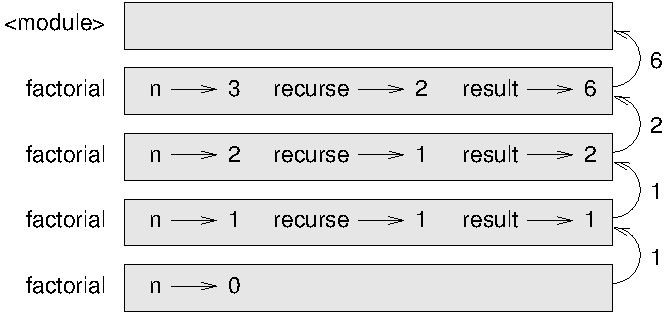
\includegraphics[scale=0.8]{figs/stack3.pdf}}
\caption{Διάγραμμα Στοίβας.}
\label{fig.stack3}
\end{figure}


Οι επιστρεφόμενες τιμές εμφανίζονται να περνάνε προς τα πίσω στη στοίβα.
Σε κάθε πλαίσιο, η επιστρεφόμενη τιμή είναι η τιμή της {\tt result} 
η οποία είναι το γινόμενο της {\tt n} με την {\tt recurse}.
\index{function frame} \index{frame}


Στο τελευταίο πλαίσιο, οι τοπικές μεταβλητές 
{\tt recurse} και {\tt result} δεν υπάρχουν γιατί
ο κλάδος που τις δημιουργεί δεν εκτελείται.


\section{Άλμα πίστης}
\index{recursion}
\index{leap of faith}

Ένας τρόπος να διαβάζουμε προγράμματα είναι να ακολουθούμε τη ροή εκτέλεσης,
το οποίο όμως μπορεί να γίνει πολύ γρήγορα λαβύρινθος. Ένας εναλλακτικός τρόπος
είναι αυτό που εγώ ονομάζω "άλμα πίστης" (leap of faith). 
Όταν βρεθείτε σε μία κλήση συνάρτησης, αντί να ακολουθήσετε τη ροή της εκτέλεσης, υποθέστε ότι η συνάρτηση δουλεύει σωστά και επιστρέφει το σωστό αποτέλεσμα.

Στην πραγματικότητα, εφαρμόζετε ήδη αυτό το άλμα πίστης όταν χρησιμοποιείτε
τις ενσωματωμένες συναρτήσεις. Όταν καλείτε την {\tt math.cos} ή 
{\tt math.exp}, δεν εξετάζετε τα σώματα αυτών των συναρτήσεων. Απλώς
θεωρείτε ότι δουλεύουν επειδή οι άνθρωποι που γράψανε τις ενσωματωμένες
συναρτήσεις ήταν καλοί προγραμματιστές.

Το ίδιο ισχύει και όταν καλείτε μία από τις δικές σας συναρτήσεις. Για
παράδειγμα, στην Ενότητα~\ref{boolean} γράψαμε μία συνάρτηση με
όνομα \verb"is_divisible" η οποία προσδιορίζει εάν ένας αριθμός
διαιρείται από έναν άλλο. Από τη στιγμή που πειστήκαμε ότι αυτή η συνάρτηση
είναι σωστή, εξετάζοντας και δοκιμάζοντας τον κώδικα, μπορούμε να χρησιμοποιήσουμε τη συνάρτηση χωρίς να ξανακοιτάξουμε το σώμα της.
\index{testing!leap of faith}

Το ίδιο ισχύει και για τα αναδρομικά προγράμματα. Όταν βρεθείτε σε μία
αναδρομική κλήση, αντί να ακολουθήσετε τη ροή της εκτέλεσης,
θεωρήστε ότι η αναδρομική κλήση δουλεύει (παράγει το σωστό αποτέλεσμα)
και στη συνέχεια αναρωτηθείτε: "Θεωρώντας ότι μπορώ να βρω το παραγοντικό
του $n-1$, μπορώ να υπολογίσω το παραγοντικό του $n$;" Σε αυτή την
περίπτωση είναι ξεκάθαρο ότι μπορείτε να το κάνετε πολλαπλασιάζοντας με $n$.

Φυσικά είναι λίγο περίεργο να θεωρούμε ότι η συνάρτηση δουλεύει σωστά
από τη στιγμή που δεν έχουμε τελειώσει το γράψιμό της, αλλά για αυτό
ονομάζεται και άλμα πίστης!


\section{Ένα ακόμα παράδειγμα}
\label{one.more.example}

\index{fibonacci function}
\index{function!fibonacci}
Το επόμενο πιο συνηθισμένο παράδειγμα, μετά το παραγοντικό, αναδρομικά οριζόμενης μαθηματικής συνάρτησης είναι το {\tt fibonacci}, του οποίου ο ορισμός είναι (βλ. \url{http://en.wikipedia.org/wiki/Fibonacci_number}):
%
\begin{eqnarray*}
&& \mathrm{fibonacci}(0) = 0 \\
&& \mathrm{fibonacci}(1) = 1 \\
&& \mathrm{fibonacci}(n) = \mathrm{fibonacci}(n-1) + \mathrm{fibonacci}(n-2)
\end{eqnarray*}
%

Γραμμένο σε Python:

\begin{verbatim}
def fibonacci(n):
    if n == 0:
        return 0
    elif  n == 1:
        return 1
    else:
        return fibonacci(n-1) + fibonacci(n-2)
\end{verbatim}
%

Αν προσπαθήσετε να ακολουθήσετε τη ροή της εκτέλεσης εδώ, ακόμα και
για αρκετά μικρές τιμές του  $n$,  το κεφάλι σας θα εκραγεί.
Αλλά σύμφωνα με το άλμα πίστης, εάν υποθέσετε ότι οι δύο αναδρομικές
κλήσεις δουλεύουν σωστά τότε είναι σαφές ότι αν τις προσθέσετε θα
πάρετε το σωστό αποτέλεσμα.
\index{flow of execution}


\section{Έλεγχος τύπων}
\label{guardian}

Τι θα συμβεί αν καλέσουμε την {\tt factorial} και της δώσουμε σαν
όρισμα 1.5;
\index{type checking}
\index{error checking}
\index{factorial function}
\index{RuntimeError}

\begin{verbatim}
>>> factorial(1.5)
RuntimeError: Maximum recursion depth exceeded
\end{verbatim}
%

Μοιάζει με άπειρη αναδρομή, αλλά πως γίνεται αυτό αφού υπάρχει μία
περίπτωση βάσης όταν {\tt n == 0}. Μπορεί να "χάσουμε" την περίπτωση βάσης αν το {\tt n} δεν είναι ακέραιος αριθμός και έτσι να έχουμε αναδρομή επ' άπειρον.
\index{infinite recursion}
\index{recursion!infinite}

Στην πρώτη αναδρομική κλήση η τιμή του {\tt n} είναι 
0.5 και στην επόμενη είναι -0.5. Από εκεί και πέρα
γίνεται όλο και μικρότερη (πιο αρνητική) αλλά ποτέ δεν θα γίνει 0.

Έχουμε δύο επιλογές. Μπορούμε να γενικεύσουμε την συνάρτηση 
{\tt factorial} για να δουλεύει και με αριθμούς κινητής υποδιαστολής
ή να την μετατρέψουμε ούτως ώστε να ελέγχει τον τύπο του ορίσματός της.
Η πρώτη επιλογή ονομάζεται συνάρτηση γάμμα και είναι εκτός του σκοπού
αυτού του βιβλίου. Επομένως θα πάμε στη δεύτερη επιλογή.
\index{gamma function}

Μπορούμε να χρησιμοποιήσουμε την ενσωματωμένη συνάρτηση {\tt isinstance} 
για να επαληθεύσουμε τον τύπο του ορίσματος. Επίσης, αφού το κάνουμε αυτό, μπορούμε να σιγουρευτούμε ότι το όρισμα είναι θετικό:
\index{isinstance function}
\index{function!isinstance}

\begin{verbatim}
def factorial (n):
    if not isinstance(n, int):
        print 'Factorial is only defined for integers.'
        return None
    elif n < 0:
        print 'Factorial is not defined for negative integers.'
        return None
    elif n == 0:
        return 1
    else:
        return n * factorial(n-1)
\end{verbatim}
%

Η πρώτη περίπτωση βάσης χειρίζεται τους μη-ακέραιους και η δεύτερη 
"συλλαμβάνει" τους αρνητικούς ακέραιους. Και στις δύο περιπτώσεις,
το πρόγραμμα εμφανίζει ένα μήνυμα λάθους και επιστρέφει 
{\tt None} για να υποδηλώσει ότι κάτι πήγε στραβά:

\begin{verbatim}
>>> factorial('fred')
Factorial is only defined for integers.
None
>>> factorial(-2)
Factorial is not defined for negative integers.
None
\end{verbatim}
%

Εάν περάσουμε και τους δύο ελέγχους, τότε ξέρουμε ότι το $n$ 
είναι είτε θετικός είτε μηδέν και άρα μπορούμε να αποδείξουμε ότι η αναδρομή
τερματίζει.
\index{guardian pattern}
\index{pattern!guardian}

Αυτό το πρόγραμμα επιδεικνύει ένα πρότυπο το οποίο μερικές φορές ονομάζεται
{\bf φύλακας} (guardian). Οι πρώτες δύο συνθήκες λειτουργούν σαν φύλακες,
προστατεύοντας τον κώδικα που ακολουθεί από τιμές οι οποίες μπορεί να προκαλέσουν σφάλμα. Οι φύλακες καθιστούν δυνατή την απόδειξη της ορθότητας του κώδικα.

Στην Ενότητα~\ref{raise} θα δούμε μία πιο ευέλικτη εναλλακτική λύση
για να εμφανίζουμε ένα μήνυμα λάθους εγείροντας μία εξαίρεση.


\section{Αποσφαλμάτωση}
\label{factdebug}

Με το σπάσιμο ενός μεγάλου προγράμματος σε συναρτήσεις δημιουργούνται
φυσικά σημεία ελέγχου για αποσφαλμάτωση. \index{debugging}
Αν μία συνάρτηση δε δουλεύει τότε πρέπει να εξετάσετε τρία ενδεχόμενα:

\begin{itemize}

\item  Κάτι πήγε στραβά με τα ορίσματα που παίρνει η συνάρτηση.
Δηλαδή παραβιάστηκε κάποια προϋπόθεση.

\item  Υπάρχει κάποιο λάθος στη συνάρτηση. Δηλαδή παραβιάστηκε κάποια 
μετασυνθήκη.

\item  Κάτι είναι λάθος με την επιστρεφόμενη τιμή ή με τον τρόπο
που χρησιμοποιήθηκε.

\end{itemize}

Για να αποκλείσετε το πρώτο ενδεχόμενο, μπορείτε να προσθέσετε μία δήλωση
{\tt print} στην αρχή της συνάρτησης και να εμφανίσετε τις τιμές των
παραμέτρων (και τους τύπους τους), ή μπορείτε να γράψετε κώδικα ο οποίος θα
ελέγχει ρητά τις προϋποθέσεις.
\index{precondition}
\index{postcondition}

Εάν οι παράμετροι φαίνονται εντάξει, προσθέστε μία δήλωση {\tt print}
πριν από κάθε δήλωση {\tt return} η οποία θα εμφανίζει την
επιστρεφόμενη τιμή. Εάν είναι εφικτό, ελέγξτε το αποτέλεσμα με το χέρι.
Δοκιμάστε να καλέσετε τη συνάρτηση με τιμές που κάνουν εύκολο τον έλεγχο
του αποτελέσματος (όπως στην Ενότητα ~\ref{incremental.development}).

Αν φαίνεται ότι η συνάρτηση δουλεύει, εξετάστε την κλήση συνάρτησης
για να σιγουρευτείτε ότι η επιστρεφόμενη τιμή χρησιμοποιείται σωστά
(ή αν χρησιμοποιείτε γενικά!)
\index{flow of execution}

Η προσθήκη δηλώσεων {\tt print} στην αρχή και στο τέλος μίας
συνάρτησης, μπορεί να κάνει πιο ορατή την ροή εκτέλεσης.
Για παράδειγμα, αυτή είναι μία έκδοση της {\tt factorial} με
δηλώσεις {\tt print}:

\begin{verbatim}
def factorial(n):
    space = ' ' * (4 * n)
    print space, 'factorial', n
    if n == 0:
        print space, 'returning 1'
        return 1
    else:
        recurse = factorial(n-1)
        result = n * recurse
        print space, 'returning', result
        return result
\end{verbatim}
%

Το {\tt space} είναι μία συμβολοσειρά από κενούς χαρακτήρες για τη
ρύθμιση των εσοχών της εξόδου. Αυτό είναι το αποτέλεσμα της {\tt factorial(5)}:

\begin{verbatim}
                     factorial 5
                 factorial 4
             factorial 3
         factorial 2
     factorial 1
 factorial 0
 returning 1
     returning 1
         returning 2
             returning 6
                 returning 24
                     returning 120
\end{verbatim}
%

Αυτού του είδους η έξοδος μπορεί να σας φανεί πολύ χρήσιμη αν σας μπερδεύει 
η ροή εκτέλεσης. Χρειάζεται κάποιο χρόνο για να φτιαχτεί μία αποτελεσματική
"σκαλωσιά", αλλά λίγη σκαλωσιά μπορεί να μας γλιτώσει από πολύ αποσφαλμάτωση.


\section{Ορολογία}

\begin{description}

\item[προσωρινή μεταβλητή:]  Μία μεταβλητή η οποία χρησιμοποιείτε για να
αποθηκεύει μία ενδιάμεση τιμή σε έναν σύνθετο υπολογισμό.
\index{temporary variable}
\index{variable!temporary}

\item[νεκρός κώδικας:]  Μέρος του κώδικα το οποίο δεν μπορεί να εκτελεστεί ποτέ, επειδή εμφανίζεται συνήθως μετά από κάποια δήλωση {\tt return}.
\index{dead code}

\item[None:]   Μία ειδική τιμή η οποία επιστρέφεται από συναρτήσεις οι
οποίες δεν έχουν καμία δήλωση επιστροφής ή έχουν δήλωση επιστροφής αλλά χωρίς
όρισμα.
\index{None special value}
\index{special value!None}

\item[σταδιακή ανάπτυξη:]  Ένα πλάνο ανάπτυξης προγραμμάτων που στοχεύει στην
αποφυγή της αποσφαλμάτωσης προσθέτοντας και δοκιμάζοντας μικρά κομμάτια
κώδικα κάθε φορά.
\index{incremental development}

\item[σκαλωσιά:]  Κώδικας ο οποίος χρησιμοποιείται κατά την ανάπτυξη ενός
προγράμματος αλλά δεν είναι μέρος της τελικής έκδοσης.
\index{scaffolding}

\item[φύλακας:]  Ένα προγραμματιστικό πρότυπο το οποίο χρησιμοποιεί δηλώσεις
υπό συνθήκη για να ελέγξει και να διαχειριστεί περιπτώσεις οι οποίες μπορεί
να προκαλέσουν κάποιο σφάλμα.
\index{guardian pattern}
\index{pattern!guardian}

\end{description}


\section{Ασκήσεις}

\begin{exercise}

Σχεδιάστε ένα διάγραμμα στοίβας για το ακόλουθο πρόγραμμα. Τι εμφανίζει το
πρόγραμμα;

Λύση: \url{http://thinkpython.com/code/stack_diagram.py}.
\index{stack diagram}

\begin{verbatim}
def b(z):
    prod = a(z, z)
    print z, prod
    return prod

def a(x, y):
    x = x + 1
    return x * y

def c(x, y, z):
    total = x + y + z
    square = b(total)**2
    return square

x = 1
y = x + 1
print c(x, y+3, x+y)

\end{verbatim}
\end{exercise}


\begin{exercise}
\label{ackermann}

Η συνάρτηση Άκερμαν, $A(m, n)$, ορίζεται:

\begin{eqnarray*}
A(m, n) = \begin{cases}
              n+1 & \mbox{if } m = 0 \\
        A(m-1, 1) & \mbox{if } m > 0 \mbox{ and } n = 0 \\
A(m-1, A(m, n-1)) & \mbox{if } m > 0 \mbox{ and } n > 0.
\end{cases}
\end{eqnarray*}
%

Βλ. \url{http://en.wikipedia.org/wiki/Ackermann_function}. 
Γράψτε μία συνάρτηση με όνομα {\tt ack} υπολογίζει τη
συνάρτηση του Άκερμαν. Χρησιμοποιήστε τη συνάρτησή σας για να
υπολογίσετε το {\tt ack(3, 4)}, το οποίο θα πρέπει να βγει 125.
Τι συμβαίνει για μεγαλύτερες τιμές του {\tt m} και του {\tt n}; 
Λύση: \url{http://thinkpython.com/code/ackermann.py}.
\index{Ackermann function}
\index{function!ack}
\\
\end{exercise}


\begin{exercise}
\label{palindrome}

Παλίνδρομο είναι μία λέξη η οποία συλλαβίζεται το ίδιο προς τα πίσω
και προς τα εμπρός, όπως είναι η  ``noon''  και η  ``redivider''. 
Αναδρομικά, μία λέξη είναι παλίνδρομο αν το πρώτο και το τελευταίο γράμμα είναι
ίδια και τα μεσαία είναι παλίνδρομο.
\index{palindrome}

Οι ακόλουθες, είναι συναρτήσεις οι οποίες παίρνουν μία συμβολοσειρά
σαν όρισμα και επιστρέφουν το πρώτο, το τελευταίο και τα μεσαία γράμματα:

\begin{verbatim}
def first(word):
    return word[0]

def last(word):
    return word[-1]

def middle(word):
    return word[1:-1]
\end{verbatim}
%

Θα δούμε πως δουλεύουν στο Κεφάλαιο~\ref{strings}.

\begin{enumerate}

\item Πληκτρολογήστε αυτές τις συναρτήσεις μέσα σε ένα αρχείο
με όνομα {\tt palindrome.py} και δοκιμάστε τες. Τι συμβαίνει
αν καλέσετε τη {\tt middle} με μία συμβολοσειρά με δύο γράμματα; 
Με ένα γράμμα; Τι γίνεται με μία κενή συμβολοσειρά, η οποία
γράφεται έτσι \verb"''" και δεν περιέχει καθόλου γράμματα;

\item Γράψτε μία συνάρτηση με όνομα \verb"is_palindrome"
η οποία θα παίρνει σαν όρισμα μία συμβολοσειρά και θα επιστρέφει 
{\tt True} εάν είναι παλίνδρομο ή {\tt False} αλλιώς.
Θυμηθείτε ότι μπορείτε να χρησιμοποιήσετε την ενσωματωμένη συνάρτηση
{\tt len} για να ελέγξετε το μήκος μίας συμβολοσειράς.

\end{enumerate}

Λύση: \url{http://thinkpython.com/code/palindrome_soln.py}.
\\
\end{exercise}


\begin{exercise}

Ένας αριθμός $a$ είναι δύναμη του $b$ εάν
διαιρείται από τον $b$ και το $a/b$ είναι δύναμη
του $b$. Γράψτε μία συνάρτηση με όνομα \verb"is_power"
η οποία θα παίρνει σαν παραμέτρους το {\tt a} και το {\tt b} 
και θα επιστρέφει {\tt True} αν το {\tt a} είναι
δύναμη του {\tt b}. 
Σημείωση: θα πρέπει να σκεφτείτε την περίπτωση βάσης.
\\
\end{exercise}


\begin{exercise}
\index{greatest common divisor (GCD)}
\index{GCD (greatest common divisor)}

Ο μέγιστος κοινός διαιρέτης (GCD) του $a$ και του $b$ 
είναι ο μεγαλύτερος αριθμός που διαιρεί και τους δύο χωρίς να αφήνει υπόλοιπο.

Ένας τρόπος για να βρούμε τον GCD δύο αριθμών είναι ο
αλγόριθμος του Ευκλείδη. Αυτός ο αλγόριθμος βασίζεται παρατήρηση ότι αν
το $r$ είναι το υπόλοιπο όταν το $a$ διαιρείται από
το $b$, τότε $gcd(a, b) = gcd(b, r)$.
Σαν περίπτωση βάσης μπορούμε να χρησιμοποιήσουμε την
$gcd(a, 0) = a$.
\index{Euclid's algorithm}
\index{algorithm!Euclid}

Γράψτε μία συνάρτηση με όνομα \verb"gcd" η οποία παίρνει
σαν παραμέτρους το {\tt a} και το {\tt b} και θα
επιστρέφει τον μέγιστο κοινό διαιρέτη τους. Για περαιτέρω βοήθεια
δείτε εδώ: \url{http://en.wikipedia.org/wiki/Euclidean_algorithm}.


Αναφορά: Αυτή η άσκηση βασίζεται σε ένα παράδειγμα του
βιβλίου {\em Structure and Interpretation of Computer Programs}
των Άμπελσον και Σούσμαν.

\end{exercise}


\chapter{Επανάληψη}

\section{Πολλαπλή εκχώρηση}
\index{assignment}
\index{statement!assignment}
\index{multiple assignment}

Ενδεχομένως να έχετε διαπιστώσει ότι είναι έγκυρο να κάνουμε περισσότερες
από μία εκχωρήσεις στην ίδια μεταβλητή. Μία νέα εκχώρηση κάνει μία μεταβλητή
να αναφέρεται σε μία νέα τιμή (και παύει η αναφορά στην παλιά τιμή). 

\begin{verbatim}
bruce = 5
print bruce,
bruce = 7
print bruce
\end{verbatim}
%

Η έξοδος αυτού του προγράμματος είναι {\tt 5 7}, επειδή την
πρώτη φορά που τυπώνεται η {\tt bruce} η τιμή της είναι 5,
ενώ τη δεύτερη φορά η τιμή της είναι 7. Το κόμμα στο τέλος της πρώτης
δήλωσης {\tt print} καταστέλλει τη νέα γραμμή και γι' αυτόν το λόγο
εμφανίζονται και οι δύο έξοδοι στην ίδια γραμμή.
\index{newline}

Η εικόνα~\ref{fig.assign2} απεικονίζει την {\bf πολλαπλή
εκχώρηση} (multiple assignmemt) σε ένα διάγραμμα κατάστασης.
\index{state diagram} \index{diagram!state}

Στην πολλαπλή εκχώρηση, είναι ιδιαίτερα σημαντικό να γίνει διάκριση
μεταξύ μίας εκχώρησης τιμής και μίας δήλωσης ισότητας. Επειδή η
Python χρησιμοποιεί το σύμβολο της ισότητας ({\tt =}) για
εκχώρηση, τυχαίνει να ερμηνεύουμε συχνά μία τέτοια δήλωση {\tt a = b}
σαν μία δήλωση ισότητας. Δεν είναι!
\index{equality and assignment}

Πρώτον, η ισότητα είναι μία συμμετρική σχέση ενώ η εκχώρηση όχι. Στα
μαθηματικά για παράδειγμα, εάν $a=7$ τότε και $7=a$. 
Στην Python όμως, ενώ η δήλωση {\tt a = 7} είναι έγκυρη,
η {\tt 7 = a} δεν είναι.

Επί πλέον, στα μαθηματικά, μία δήλωση ισότητας είναι είτε αληθής είτε
ψευδής για πάντα. Αν $a=b$ τώρα, τότε το $a$ θα είναι
πάντα ίσο με το $b$. Στην Python, μία δήλωση εκχώρησης
μπορεί να κάνει δύο μεταβλητές ίσες αλλά δεν είναι απαραίτητο 
ότι θα μείνουν πάντα έτσι:

\begin{verbatim}
a = 5
b = a    # a and b are now equal
a = 3    # a and b are no longer equal
\end{verbatim}
%

Η τρίτη γραμμή αλλάζει την τιμή της {\tt a} αλλά δεν αλλάζει
την τιμή της {\tt b} και επομένως δεν είναι πλέον ίσες.

Παρόλο που η πολλαπλή εκχώρηση είναι συχνά χρήσιμη, θα πρέπει να τη
χρησιμοποιείτε με προσοχή. Μπορεί να δυσκολέψει η ανάγνωση και η αποσφαλμάτωση του κώδικα αν αλλάζουν συχνά οι τιμές των μεταβλητών.

\begin{figure}
\centerline
{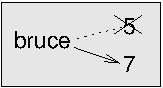
\includegraphics[scale=0.8]{figs/assign2.pdf}}
\caption{Διάγραμμα κατάστασης.}
\label{fig.assign2}
\end{figure}


\section{Ενημέρωση μεταβλητών}
\label{update}

\index{update}
\index{variable!updating}

Μία από τις συχνότερες μορφές της πολλαπλής εκχώρησης είναι η {\bf ενημέρωση} (update), όπου η νέα τιμή της μεταβλητής εξαρτάται από την παλιά:

\begin{verbatim}
x = x+1
\end{verbatim}
%

Αυτό σημαίνει: "πάρε την τιμή του {\tt x}, πρόσθεσε ένα και
μετά ενημέρωσε το {\tt x} με τη νέα τιμή".

Αν προσπαθήσετε να ενημερώσετε μία μεταβλητή η οποία δεν υπάρχει, τότε θα πάρετε μήνυμα λάθους. Αυτό συμβαίνει επειδή η Python υπολογίζει πρώτα το δεξιό μέρος πριν εκχωρήσει την τιμή στο {\tt x}:

\begin{verbatim}
>>> x = x+1
NameError: name 'x' is not defined
\end{verbatim}
%

Για να είστε σε θέση να ενημερώσετε μία μεταβλητή, θα πρέπει πρώτα να την
{\bf αρχικοποιήσετε} (initialize) και αυτό συνήθως γίνεται με μία απλή εκχώρηση:
\index{initialization (before update)}

\begin{verbatim}
>>> x = 0
>>> x = x+1
\end{verbatim}
%

Η ενημέρωση μίας μεταβλητής προσθέτοντας της 1 ονομάζεται {\bf προσαύξηση},
ενώ αφαιρώντας 1 ονομάζεται {\bf μείωση} (decrement) της μεταβλητής.
\index{increment}
\index{decrement}




\section{Η δήλωση \tt while}
\index{statement!while}
\index{while loop}
\index{loop!while}
\index{iteration}


Οι υπολογιστές χρησιμοποιούνται συχνά για την αυτοματοποίηση επαναλαμβανόμενων
εργασιών. Η επανάληψη πανομοιότυπων ή παρόμοιων εργασιών χωρίς λάθη είναι
εύκολη υπόθεση για τους υπολογιστές αλλά δεν ισχύει το ίδιο και για τους ανθρώπους.

Έχουμε δει δύο προγράμματα, το {\tt countdown} και το \verb"print_n",
τα οποία χρησιμοποιούν αναδρομή για να εκτελέσουν {\bf επανάληψη} (iteration/repetition). Επειδή η επανάληψη χρησιμοποιείται συχνά, η Python παρέχει διάφορες λειτουργίες για να την κάνει ευκολότερη. Μία από αυτές είναι η δήλωση {\tt for} που είδαμε στην Ενότητα~\ref{repetition} και
θα επανέλθουμε σε αυτήν αργότερα.

Μία άλλη είναι η δήλωση {\tt while}. Αυτή είναι μία έκδοση
της {\tt countdown} η οποία χρησιμοποιεί μία δήλωση {\tt while}:

\begin{verbatim}
def countdown(n):
    while n > 0:
        print n
        n = n-1
    print 'Blastoff!'
\end{verbatim}
%

Η δήλωση {\tt while} διαβάζεται σχεδόν σαν να μία πρόταση στα Αγγλικά.
Αυτό σημαίνει ότι : " Όσο το {\tt n} είναι μεγαλύτερο του 0,
εμφάνισε την τιμή του {\tt n} και στη συνέχεια μείωσε την τιμή του κατά 1.
Όταν φτάσεις στο 0, εμφάνισε τη λέξη {\tt Blastoff}!"
\index{flow of execution}

Πιο επίσημα, η ροή εκτέλεσης για μία δήλωση {\tt while} είναι η εξής :

\begin{enumerate}

\item Αξιολόγησε τη συνθήκη επιστρέφοντας {\tt True} ή {\tt False}.

\item Αν η συνθήκη είναι ψευδής, βγες από τη δήλωση  {\tt while}  και συνέχισε με την εκτέλεση της επόμενης δήλωσης.

\item Αν η συνθήκη είναι αληθής, εκτέλεσε το σώμα και μετά επέστρεψε στο πρώτο βήμα.

\end{enumerate}

Αυτός ο τύπος ροής ονομάζεται {\bf βρόχος} (loop) επειδή το
τρίτο βήμα επιστρέφει τη ροή στην αρχή.
\index{condition}
\index{loop}
\index{body}

Το σώμα του βρόχου θα πρέπει να αλλάζει την τιμή ενός ή περισσοτέρων
μεταβλητών έτσι ώστε τελικά η συνθήκη να γίνει ψευδής και να τερματίσει
ο βρόχος. Σε οποιαδήποτε άλλη περίπτωση, ο βρόχος θα επαναλαμβάνεται επ' άπειρον και ένας τέτοιος βρόχος ονομάζεται {\bf ατέρμων βρόχος} (infinite loop). Μία ατέλειωτη πηγή διασκέδασης για τους επιστήμονες της
πληροφορικής είναι η παρατήρηση ότι οι οδηγίες για ένα σαμπουάν, 
"Σαπουνίστε, ξεπλύνετε και επαναλάβετε", αποτελούν έναν ατέρμων βρόχο.
\index{infinite loop}
\index{loop!infinite}

Στην περίπτωση της {\tt countdown}, μπορούμε να αποδείξουμε ότι ο
βρόχος τερματίζει επειδή ξέρουμε ότι η τιμή του {\tt n} είναι πεπερασμένη,
και μπορούμε να δούμε ότι η τιμή του μειώνεται σε κάθε επανάληψη του βρόχου, έτσι ώστε τελικά να πάρει την τιμή 0. Σε άλλες περιπτώσεις όμως δεν είναι τόσο εύκολο:

\begin{verbatim}
def sequence(n):
    while n != 1:
        print n,
        if n%2 == 0:        # n is even
            n = n/2
        else:               # n is odd
            n = n*3+1
\end{verbatim}
%

Η συνθήκη για αυτό το βρόχο είναι η {\tt n != 1}, άρα ο βρόχος
συνεχίζει να εκτελείται μέχρι το {\tt n} να γίνει {\tt 1},
το οποίο θα κάνει τη συνθήκη ψευδή.

Σε κάθε επανάληψη, το πρόγραμμα εμφανίζει την τιμή του {\tt n} 
και ελέγχει εάν είναι άρτιος ή περιττός. Αν είναι άρτιος, το {\tt n} 
διαιρείται με το 2. Αν είναι περιττός, η τιμή του {\tt n} αντικαθίσταται
με {\tt n*3+1}. Για παράδειγμα, αν περάσουμε το 3 σαν όρισμα στην
{\tt sequence}, η σειρά των αποτελεσμάτων θα είναι: 3, 10, 5, 16, 8, 4, 2, 1.

Από τη στιγμή που το {\tt n} άλλες φορές αυξάνεται και άλλες φορές
μειώνεται, δεν υπάρχει κάποια προφανής απόδειξη ότι το {\tt n} θα γίνει
κάποια στιγμή ίσο με 1, ή ότι το πρόγραμμα τερματίζει. Για κάποιες συγκεκριμένες τιμές του {\tt n}, μπορούμε να αποδείξουμε τον τερματισμό του προγράμματος. Για παράδειγμα, αν η αρχική τιμή του {\tt n} είναι μία δύναμη του δύο, τότε η τιμή του {\tt n} σε κάθε επανάληψη θα είναι άρτια μέχρι να γίνει ίση με 1. Το προηγούμενο παράδειγμα τελειώνει με μία τέτοια ακολουθία, ξεκινώντας με 16.
\index{Collatz conjecture}

Το δύσκολο είναι να αποδείξουμε ότι το πρόγραμμα τερματίζει για οποιαδήποτε
θετική τιμή του {\tt n}. Μέχρι στιγμής, κανείς δεν μπόρεσε να το αποδείξει αλλά 
ούτε και να το διαψεύσει! (Βλ.\url{http://en.wikipedia.org/wiki/Collatz_conjecture}).
\\
\begin{exercise}

Ξαναγράψτε τη συνάρτηση \verb"print_n" της Ενότητας~\ref{recursion} 
χρησιμοποιώντας επανάληψη αντί για αναδρομή.
\end{exercise}


\section{Η δήλωση \tt break}
\index{break statement}
\index{statement!break}


Μερικές φορές δεν ξέρετε ότι ήρθε η ώρα για να τερματίσει ένας βρόχος μέχρι να
φτάσετε στη μέση του σώματός του. Σε αυτήν την περίπτωση μπορείτε να χρησιμοποιήσετε τη δήλωση {\tt break} για να βγείτε έξω από το βρόχο.

Για παράδειγμα, υποθέστε ότι θέλετε να δέχεστε είσοδο από το χρήστη μέχρις ότου
πληκτρολογήσει {\tt done}. Μπορείτε να γράψετε:

\begin{verbatim}
while True:
    line = raw_input('> ')
    if line == 'done':
        break
    print line

print 'Done!'
\end{verbatim}
%

Η συνθήκη τερματισμού του βρόχου είναι η {\tt True}, η οποία είναι
πάντα αληθής, και άρα ο βρόχος εκτελείται μέχρι να φτάσει στην δήλωση break.

Σε κάθε επανάληψη, ζητάει είσοδο από το χρήστη με το σύμβολο '>'.
Αν ο χρήστης πληκτρολογήσει {\tt done}, τότε βγαίνει από το βρόχο με τη δήλωση
{\tt break}. Αλλιώς, το πρόγραμμα εμφανίζει ότι πληκτρολογεί ο χρήστης και
επιστρέφει στην αρχή του βρόχου. Αυτό είναι ένα δείγμα εκτέλεσης:

\begin{verbatim}
> not done
not done
> done
Done!
\end{verbatim}
%

Αυτός ο τρόπος γραφής βρόχων {\tt while} είναι πολύ κοινός
επειδή μπορείτε να ελέγξετε τη συνθήκη οπουδήποτε μέσα στο βρόχο (όχι
μόνο στην αρχή) και επίσης μπορείτε να εκφράσετε τη συνθήκη τερματισμού
καταφατικά (σταμάτα όταν συμβεί αυτό) αντί για αρνητικά
(συνέχισε μέχρι να συμβεί αυτό).


\section{Τετραγωνικές ρίζες}
\label{squareroot}
\index{square root}

Οι βρόχοι χρησιμοποιούνται συχνά σε προγράμματα τα οποία
υπολογίζουν αριθμητικά αποτελέσματα αρχίζοντας με μία κατά προσέγγιση 
απάντηση την οποία βελτιώνουν σε κάθε επανάληψη.
\index{Newton's method}

Για παράδειγμα, ένας τρόπος υπολογισμού της τετραγωνικής ρίζας ενός αριθμού
είναι η μέθοδος του Νιούτον. Υποθέστε ότι θέλετε να υπολογίσετε την τετραγωνική ρίζα του $a$. Αν ξεκινήσετε με σχεδόν οποιαδήποτε εκτίμηση $x$, τότε μπορείτε
να υπολογίσετε μία καλύτερη εκτίμηση με βάση τον ακόλουθο τύπο:

\[ y = \frac{x + a/x}{2} \]
%

Για παράδειγμα, αν το $a$ είναι 4 και το $x$ είναι 3:

\begin{verbatim}
>>> a = 4.0
>>> x = 3.0
>>> y = (x + a/x) / 2
>>> print y
2.16666666667
\end{verbatim}
%

Το οποίο είναι πιο κοντά στη σωστή απάντηση ($\sqrt{4} = 2$). Αν
επαναλάβουμε τη διαδικασία με τη νέα εκτίμηση, τότε πλησιάζουμε ακόμα περισσότερο:

\begin{verbatim}
>>> x = y
>>> y = (x + a/x) / 2
>>> print y
2.00641025641
\end{verbatim}
%

Μετά από μερικές ακόμα ενημερώσεις, η εκτίμηση είναι σχεδόν ακριβής:
\index{update}

\begin{verbatim}
>>> x = y
>>> y = (x + a/x) / 2
>>> print y
2.00001024003
>>> x = y
>>> y = (x + a/x) / 2
>>> print y
2.00000000003
\end{verbatim}
%

Σε γενικές γραμμές δεν γνωρίζουμε εκ των προτέρων πόσα βήματα θα χρειαστούμε
για να φτάσουμε στη σωστή απάντηση, αλλά ξέρουμε ότι φτάσαμε όταν η εκτίμηση
σταματήσει να αλλάζει:

\begin{verbatim}
>>> x = y
>>> y = (x + a/x) / 2
>>> print y
2.0
>>> x = y
>>> y = (x + a/x) / 2
>>> print y
2.0
\end{verbatim}
%

Όταν {\tt y == x}, τότε μπορούμε να σταματήσουμε. Ακολουθεί ένας βρόχος ο
οποίος ξεκινάει με μία αρχική εκτίμηση {\tt x}, και τη βελτιώνει μέχρι
να σταματήσει να αλλάζει:

\begin{verbatim}
while True:
    print x
    y = (x + a/x) / 2
    if y == x:
        break
    x = y
\end{verbatim}
%

Για τις περισσότερες τιμές του {\tt a} δουλεύει καλά, αλλά γενικά
είναι επίφοβο να ελέγχουμε την ισότητα δεκαδικών αριθμών. Οι τιμές των αριθμών
κινητής υποδιαστολής είναι σωστές μόνο κατά προσέγγιση. Οι περισσότεροι ρητοί
όπως το  $1/3$  και άρρητοι αριθμοί όπως η  $\sqrt{2}$  δεν μπορούν
να αναπαρασταθούν με ακρίβεια από μία {\tt float} μεταβλητή.
\index{floating-point}
\index{epsilon}

Αντί να ελέγχουμε αν το {\tt x} και το {\tt y} είναι ακριβώς ίσα,
είναι ασφαλέστερο να χρησιμοποιούμε την ενσωματωμένη συνάρτηση  {\tt abs}  για
υπολογίσουμε την απόλυτη τιμή ή το μέγεθος της διαφοράς τους:

\begin{verbatim}
    if abs(y-x) < epsilon:
        break
\end{verbatim}
%

Όπου \verb"epsilon", είναι μία τιμή όπως η {\tt 0.0000001} 
η οποία καθορίζει πόσο κοντά είναι αρκετά κοντά.
\\
\begin{exercise}

Ενθυλακώστε αυτό το βρόχο σε μία συνάρτηση με όνομα \verb"square_root" 
η οποία θα παίρνει το {\tt a} σαν παράμετρο, θα επιλέγει μία λογική
τιμή του {\tt x} και θα επιστρέφει μία εκτίμηση της τετραγωνικής ρίζας του
{\tt a}.
\end{exercise}


\section{Αλγόριθμοι}
\index{algorithm}

Η μέθοδος του Νιούτον αποτελεί ένα παράδειγμα ενός {\bf αλγορίθμου}: 
μία μηχανική διαδικασία για την επίλυση μίας κατηγορίας προβλημάτων
(σε αυτήν την περίπτωση, ο υπολογισμός της τετραγωνικής ρίζας ενός αριθμού).

Δεν είναι εύκολο να οριστεί ένας αλγόριθμος. Θα σας βοηθούσε εάν ξεκινούσατε με κάτι το οποίο δεν είναι αλγόριθμος. Όταν μάθατε να πολλαπλασιάζετε μονοψήφιους αριθμούς, τότε μάλλον απομνημονεύσατε και την προπαίδεια. Και έτσι, απομνημονεύσατε 100 συγκεκριμένες λύσεις. Αυτού του τύπου η γνώση δεν είναι αλγόριθμος.

Αν ήσασταν όμως "τεμπέληδες", τότε μάλλον κάνατε ζαβολιές μαθαίνοντας μερικά κόλπα. Για παράδειγμα, για να βρείτε το γινόμενο του $n$ με το 9, μπορείτε να γράψετε $n-1$ για το πρώτο ψηφίο και $10-n$ για το δεύτερο. Αυτό το κόλπο είναι μία γενική λύση για τον πολλαπλασιασμό ενός οποιουδήποτε μονοψήφιου αριθμού με το 9. Και αυτό είναι ένας αλγόριθμος!
\index{addition with carrying}
\index{carrying, addition with}
\index{subtraction!with borrowing}
\index{borrowing, subtraction with}

Ομοίως, οι τεχνικές που μάθατε για την πρόσθεση με κρατούμενο, την αφαίρεση με
δανεισμό και τη διαίρεση είναι όλες αλγόριθμοι. Ένα από τα χαρακτηριστικά των
αλγορίθμων είναι ότι δεν απαιτούν ευφυΐα για να εκτελεστούν. Είναι μηχανικές διαδικασίες στις οποίες κάθε βήμα απορρέει από το προηγούμενο με βάση ένα απλό σύνολο κανόνων.

Κατά τη γνώμη μου, είναι πολύ δυσάρεστο το γεγονός ότι οι άνθρωποι ξοδεύουν τόσο πολύ χρόνο στα σχολεία για να μάθουν να εκτελούν αλγόριθμους. Είναι μία διαδικασία που στην κυριολεξία δεν χρειάζεται καθόλου ευφυΐα.

Από την άλλη πλευρά, η διαδικασία του σχεδιασμού αλγορίθμων είναι μία ενδιαφέρουσα πνευματική πρόκληση η οποία αποτελεί βασικό κομμάτι αυτού που ονομάζουμε προγραμματισμό.

Μερικά από τα πράγματα τα οποία οι άνθρωποι κάνουν φυσικά, χωρίς δυσκολία ή συνειδητή σκέψη, είναι πολύ δύσκολο να εκφραστούν αλγοριθμικά. Ένα καλό παράδειγμα είναι η κατανόηση μίας φυσικής γλώσσας. Αυτό το κάνουμε όλοι, αλλά μέχρι στιγμής κανένας δεν ήταν σε θέση να εξηγήσει "πως" το κάνουμε ή τουλάχιστον όχι με τη μορφή αλγόριθμου.


\section{Αποσφαλμάτωση}

Όσο θα γράφετε όλο και μεγαλύτερα προγράμματα, τόσο θα διαπιστώνετε ότι αφιερώνετε όλο και περισσότερο χρόνο για αποσφαλμάτωση. Γράφοντας περισσότερο κώδικα αυξάνονται οι πιθανότητες να κάνετε κάποιο λάθος μιας και υπάρχει περισσότερος χώρος για να κρυφτούν τα σφάλματα.
\index{debugging!by bisection}
\index{bisection, debugging by}

Ένας τρόπος για να μειώσετε το χρόνο αποσφαλμάτωσης είναι η "αποσφαλμάτωση με
διχοτόμηση". Για παράδειγμα, αν υπάρχουν 100 γραμμές στο πρόγραμμά σας και εσείς τις ελέγχατε όλες μία μία, τότε θα χρειαζόσασταν 100 βήματα.

Αντ' αυτού, δοκιμάστε να σπάσετε το πρόγραμμα στη μέση. Ψάξτε στη μέση του προγράμματος, ή κάπου κοντά σε αυτήν, για μία ενδιάμεση τιμή την οποία μπορείτε να ελέγξετε. Προσθέστε μία δήλωση {\tt print} (ή κάτι άλλο το οποίο θα έχει επαληθεύσιμη επίδραση) και τρέξτε το πρόγραμμα.

Εάν αυτό το σημείο ελέγχου στη μέση είναι εσφαλμένο, τότε πρέπει να υπάρχει λάθος στο πρώτο μισό του προγράμματος. Αν είναι σωστό, τότε το πρόβλημα είναι στο δεύτερο μισό.

Κάθε φορά που εκτελείτε έναν τέτοιο έλεγχο, μειώνετε κατά το ήμισυ τις γραμμές που πρέπει να ψάξετε για να βρείτε το λάθος. Θεωρητικά, μετά από έξι βήματα (τα οποία είναι λιγότερα από 100) θα είστε στη μία ή δύο γραμμές του κώδικα που βρίσκετε το λάθος.

Στην πράξη, δεν είναι πάντα ξεκάθαρο ποια είναι η "μέση του προγράμματος" και ίσως να μην είναι και εφικτό να τη βρούμε. Δεν έχει νόημα να μετράμε γραμμές για να βρούμε ακριβώς το σημείο της μέσης. Αντ' αυτού, ψάξτε για περιοχές στο κώδικα που μπορεί να υπάρχουν λάθη και σημεία που είναι εύκολο να βάλετε έναν έλεγχο. Και στη συνέχεια διαλέξτε ένα σημείο όπου οι πιθανότητες, για
το σφάλμα να είναι πριν ή μετά του σημείου ελέγχου, είναι περίπου ίδιες.




\section{Ορολογία}

\begin{description}

\item[πολλαπλή εκχώρηση:] Το να γίνονται περισσότερες από μία εκχωρήσεις τιμής στην ίδια μεταβλητή
κατά την εκτέλεση του προγράμματος.
\index{multiple assignment}
\index{assignment!multiple}

\item[ενημέρωση:] Μία εκχώρηση όπου η νέα τιμή της μεταβλητής εξαρτάται από την παλιά.
\index{update}

\item[αρχικοποίηση:] Μία εκχώρηση η οποία δίνει αρχική τιμή σε μία μεταβλητή η οποία θα ενημερωθεί.
\index{initialization!variable}

\item[προσαύξηση:] Μία ενημέρωση η οποία αυξάνει την τιμή μίας μεταβλητής (συνήθως κατά ένα).
\index{increment}

\item[μείωση:] Μία ενημέρωση η οποία μειώνει την τιμή μίας μεταβλητής.
\index{decrement}

\item[επανάληψη:] Επαναλαμβανόμενη εκτέλεση ενός συνόλου δηλώσεων χρησιμοποιώντας είτε μία αναδρομική συνάρτηση είτε έναν βρόχο.
\index{iteration}

\item[ατέρμων βρόχος:] Ένας βρόχος στον οποίο η συνθήκη τέλους δεν ικανοποιείται ποτέ.
\index{infinite loop}

\end{description}


\section{Ασκήσεις}

\begin{exercise}
\index{algorithm!square root}

Για να ελέγξετε τον αλγόριθμο υπολογισμού τετραγωνικής ρίζας αυτού του κεφαλαίου, μπορείτε να τον συγκρίνετε με τη {\tt math.sqrt}. Γράψτε μία συνάρτηση με όνομα \verb"test_square_root" η οποία θα εμφανίζει στην οθόνη έναν τέτοιο πίνακα :

\begin{verbatim}
1.0 1.0           1.0           0.0
2.0 1.41421356237 1.41421356237 2.22044604925e-16
3.0 1.73205080757 1.73205080757 0.0
4.0 2.0           2.0           0.0
5.0 2.2360679775  2.2360679775  0.0
6.0 2.44948974278 2.44948974278 0.0
7.0 2.64575131106 2.64575131106 0.0
8.0 2.82842712475 2.82842712475 4.4408920985e-16
9.0 3.0           3.0           0.0

\end{verbatim}
%

Η πρώτη στήλη είναι ένας αριθμός $a$, η δεύτερη είναι η τετραγωνική
ρίζα του $a$ υπολογισμένη με τη συνάρτηση της Ενότητα~\ref{squareroot}, 
η τρίτη στήλη είναι η τετραγωνική ρίζα υπολογισμένη από τη {\tt math.sqrt},  και η τέταρτη στήλη είναι η απόλυτη τιμή της διαφοράς μεταξύ των δύο υπολογισθέντων τιμών.
\\
\end{exercise}


\begin{exercise}
\index{eval function}
\index{function!eval}

Η ενσωματωμένη συνάρτηση {\tt eval} παίρνει μία συμβολοσειρά σαν όρισμα και την
υπολογίζει χρησιμοποιώντας τον διερμηνέα της Python. Για παράδειγμα:

\begin{verbatim}
>>> eval('1 + 2 * 3')
7
>>> import math
>>> eval('math.sqrt(5)')
2.2360679774997898
>>> eval('type(math.pi)')
<type 'float'>
\end{verbatim}
%

Γράψτε μία συνάρτηση με όνομα \verb"eval_loop" η οποία προτρέπει
επαναληπτικά τον χρήστη, παίρνει την είσοδο και την υπολογίζει χρησιμοποιώντας
την {\tt eval} και μετά εμφανίζει το αποτέλεσμα.

Θα πρέπει να συνεχίζει μέχρι ο χρήστης να πληκτρολογήσει \verb"'done'" και
στη συνέχεια να επιστρέφει την τελευταία έκφραση που υπολόγισε.
\\
\end{exercise}


\begin{exercise}
\index{Ramanujan, Srinivasa}

Ο μαθηματικός Σρινιβάσα Ραμανούτζαν βρήκε μία άπειρη σειρά η οποία μπορεί να
χρησιμοποιηθεί για να παράγει μία αριθμητική προσέγγιση του $\pi$:
\index{pi}

\[ \frac{1}{\pi} = \frac{2\sqrt{2}}{9801}
\sum^\infty_{k=0} \frac{(4k)!(1103+26390k)}{(k!)^4 396^{4k}} \]


Γράψτε μία συνάρτηση με όνομα \verb"estimate_pi" η οποία θα χρησιμοποιεί αυτόν
τον τύπο για να υπολογίσει και να επιστρέψει μία εκτίμηση του $\pi$. Θα πρέπει
να χρησιμοποιεί έναν βρόχο {\tt while} για να υπολογίζει τους όρους της άθροισης μέχρι ο τελευταίος όρος να είναι μικρότερος του {\tt 1e-15} (ο οποίος είναι ο τρόπος συμβολισμού του $10^{-15}$ στην Python). Μπορείτε να ελέγξετε το αποτέλεσμα συγκρίνοντάς το με την {\tt math.pi}.

Λύση: \url{http://thinkpython.com/code/pi.py}.

\end{exercise}



\chapter{Συμβολοσειρές}
\label{strings}


\section{Μία συμβολοσειρά είναι μία ακολουθία}

\index{sequence}
\index{character}
\index{bracket operator}
\index{operator!bracket}
Μία συμβολοσειρά είναι μία ακολουθία χαρακτήρων.
Μπορείτε να έχετε πρόσβαση στους χαρακτήρες (έναν τη φορά) με τους
τελεστές αγκύλης:

\begin{verbatim}
>>> fruit = 'banana'
>>> letter = fruit[1]
\end{verbatim}
%

Η δεύτερη δήλωση επιλέγει το χαρακτήρα νούμερο 1 από τη μεταβλητή 
{\tt fruit} και τον εκχωρεί στη μεταβλητή {\tt letter}.
\index{index}

Η έκφραση μέσα στις αγκύλες ονομάζεται {\bf δείκτης} (index). 
Ο δείκτης υποδεικνύει ποιον χαρακτήρα της ακολουθίας θέλετε (εξού και το όνομα).

Το αποτέλεσμα όμως μπορεί να μην είναι που θα περιμένατε:

\begin{verbatim}
>>> print letter
a
\end{verbatim}
%

Για τους περισσότερους ανθρώπους, το πρώτο γράμμα της λέξης \verb"'banana'"
είναι το {\tt b} και όχι το {\tt a}. Αλλά για τους επιστήμονες των υπολογιστών,
ο δείκτης είναι η απόκλιση από την αρχή της συμβολοσειράς και άρα η απόκλιση του πρώτου γράμματος είναι μηδέν.  

\begin{verbatim}
>>> letter = fruit[0]
>>> print letter
b
\end{verbatim}
%

Άρα το {\tt b} είναι το 0ο γράμμα της λέξης \verb"'banana'", το
{\tt a} είναι το 1ο γράμμα και το {\tt n} είναι το 2ο γράμμα.
\index{index!starting at zero}
\index{zero, index starting at}

Μπορείτε να χρησιμοποιήσετε οποιαδήποτε έκφραση, συμπεριλαμβανομένων μεταβλητών και τελεστών, σαν δείκτη, αλλά η τιμή του δείκτη πρέπει να είναι ακέραιος αριθμός. Αλλιώς θα πάρετε:
\index{index}
\index{exception!TypeError}
\index{TypeError}

\begin{verbatim}
>>> letter = fruit[1.5]
TypeError: string indices must be integers
\end{verbatim}
%


\section{Η δήλωση \tt len}
\index{len function}
\index{function!len}


Η συνάρτηση {\tt len} είναι μία ενσωματωμένη συνάρτηση η οποία επιστρέφει
το πλήθος των χαρακτήρων μίας συμβολοσειράς:

\begin{verbatim}
>>> fruit = 'banana'
>>> len(fruit)
6
\end{verbatim}
%

Εάν θέλατε να πάρετε το τελευταίο γράμμα μίας συμβολοσειράς, ενδεχομένως να μπαίνατε στον πειρασμό να δοκιμάσετε κάτι τέτοιο:
\index{exception!IndexError}
\index{IndexError}

\begin{verbatim}
>>> length = len(fruit)
>>> last = fruit[length]
IndexError: string index out of range
\end{verbatim}
%

Το σφάλμα {\tt IndexError} οφείλεται στο γεγονός ότι δεν υπάρχει κανένα γράμμα
στη λέξη {\tt 'banana'} με δείκτη 6. Από τη στιγμή που αρχίζουμε να μετράμε από το μηδέν, τα έξι γράμματα αριθμούνται από το 0 ως το 5. Για να πάρετε τον τελευταίο χαρακτήρα θα πρέπει να αφαιρέσετε 1 από την {\tt length}:

\begin{verbatim}
>>> last = fruit[length-1]
>>> print last
a
\end{verbatim}
%

Εναλλακτικά, μπορείτε να χρησιμοποιήσετε αρνητικούς δείκτες, οι οποίοι μετρούν προς τα πίσω από το τέλος της συμβολοσειράς. Η έκφραση {\tt fruit[-1]} επιστρέφει το τελευταίο γράμμα, η {\tt fruit[-2]} το προτελευταίο και ούτω καθεξής.
\index{index!negative}
\index{negative index}


\section{Διάσχιση με {\tt for}}
\label{for}
\index{traversal}
\index{loop!traversal}
\index{for loop}
\index{loop!for}
\index{statement!for}
\index{traversal}

Πολλοί υπολογισμοί περιλαμβάνουν επεξεργασία συμβολοσειράς χρησιμοποιώντας ένα χαρακτήρα τη φορά. Συνήθως ξεκινάνε από την αρχή επιλέγοντας και χρησιμοποιώντας κάθε χαρακτήρα με τη σειρά μέχρι το τέλος. Αυτό το πρότυπο επεξεργασίας ονομάζεται {\bf διάσχιση} (traversal). Μπορούμε να γράψουμε μία διάσχιση χρησιμοποιώντας ένα βρόχο {\tt while}:

\begin{verbatim}
index = 0
while index < len(fruit):
    letter = fruit[index]
    print letter
    index = index + 1
\end{verbatim}
%

Αυτός ο βρόχος διασχίζει τη συμβολοσειρά και εμφανίζει κάθε γράμμα της σε μία γραμμή. Η συνθήκη του βρόχου είναι η {\tt index < len(fruit)}, έτσι ώστε όταν ο δείκτης {\tt index} γίνει ίσος με το μήκος της συμβολοσειράς η συνθήκη γίνεται ψευδής και παύει να εκτελείται το σώμα του βρόχου. Ο τελευταίος χαρακτήρας που θα προσπελαστεί είναι αυτός με δείκτη {\tt len(fruit)-1}, ο οποίος είναι και ο τελευταίος χαρακτήρας της συμβολοσειράς.
\\
\begin{exercise}

Γράψτε μία συνάρτηση η οποία θα παίρνει μία συμβολοσειρά σαν όρισμα
και θα εμφανίζει όλα τα γράμματά της με τη σειρά, ένα σε κάθε γραμμή,
ξεκινώντας από το τελευταίο.
\end{exercise}

Ένας άλλος τρόπος για να γράψουμε μία διάσχιση είναι με έναν βρόχο {\tt for}:

\begin{verbatim}
for char in fruit:
    print char
\end{verbatim}
%

Σε κάθε επανάληψη του βρόχου, ο επόμενος χαρακτήρας της συμβολοσειράς εκχωρείται στη μεταβλητή {\tt char}. Ο βρόχος εκτελείται μέχρις ότου να μην υπάρχουν άλλοι χαρακτήρες.
\index{concatenation}
\index{abecedarian}
\index{McCloskey, Robert}

Το παρακάτω παράδειγμα δείχνει πως χρησιμοποιείται η συνένωση (πρόσθεση συμβολοσειρών) και ένας βρόχος {\tt for} για να παραχθεί μία αλφαβητικά ταξινομημένη σειρά. Στο βιβλίο του Ρόμπερτ ΜακΚλάσκι {\em Make Way for Ducklings}, τα ονόματα από τα παπάκια είναι Jack, Kack, Lack, Mack, Nack, Ouack, Pack, and Quack. Αυτός ο βρόχος έχει σαν έξοδο αυτά τα ονόματα με τη σειρά:

\begin{verbatim}
prefixes = 'JKLMNOPQ'
suffix = 'ack'

for letter in prefixes:
    print letter + suffix
\end{verbatim}
%

Η έξοδος είναι:

\begin{verbatim}
Jack
Kack
Lack
Mack
Nack
Oack
Pack
Qack
\end{verbatim}
%

Αυτό φυσικά δεν είναι και πολύ σωστό αφού το ``Ouack'' και το ``Quack'' 
έχουν ορθογραφικό λάθος.
\\
\begin{exercise}

Τροποποιήστε το πρόγραμμα ούτως ώστε να διορθώσετε αυτό το λάθος.
\end{exercise}


\section{Τεμάχια συμβολοσειράς}
\label{slice}
\index{slice operator}
\index{operator!slice}
\index{index!slice}
\index{string!slice}
\index{slice!string}

Ένα τμήμα μίας συμβολοσειράς ονομάζεται {\bf τεμάχιο} (slice). Η επιλογή ενός
τεμαχίου είναι παρόμοια με την επιλογή ενός χαρακτήρα:

\begin{verbatim}
>>> s = 'Monty Python'
>>> print s[0:5]
Monty
>>> print s[6:12]
Python
\end{verbatim}
%

Ο τελεστής {\tt [n:m]} επιστρέφει το τμήμα της συμβολοσειράς από το
n οστό έως το m οστό χαρακτήρα, συμπεριλαμβανομένου του πρώτου αλλά όχι και
του τελευταίου. Αυτή η συμπεριφορά είναι κάπως αντιφατική, αλλά ίσως σας βοηθήσει να φανταστείτε πως δείχνουν οι δείκτες ανάμεσα στους χαρακτήρες, όπως στην Εικόνα~\ref{fig.banana}.

\begin{figure}
\centerline
{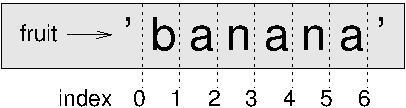
\includegraphics[scale=0.8]{figs/banana.pdf}}
\caption{Δείκτες τεμαχίων.}
\label{fig.banana}
\end{figure}


Εάν παραλείψετε τον πρώτο δείκτη (πριν την άνω κάτω τελεία), τότε το τεμάχιο θα ξεκινήσει από την αρχή της συμβολοσειράς. Αν παραλείψετε τον δεύτερο δείκτη, τότε το τεμάχιο θα φτάσει μέχρι το τέλος της συμβολοσειράς:

\begin{verbatim}
>>> fruit = 'banana'
>>> fruit[:3]
'ban'
>>> fruit[3:]
'ana'
\end{verbatim}
%

Αν ο πρώτος δείκτης είναι μεγαλύτερος ή ίσος με το δεύτερο το αποτέλεσμα θα είναι μία {\bf κενή συμβολοσειρά} (empty string), η οποία αναπαριστάται από δύο μονά εισαγωγικά:
\index{quotation mark}

\begin{verbatim}
>>> fruit = 'banana'
>>> fruit[3:3]
''
\end{verbatim}
%

Αν εξαιρέσουμε ότι μία κενή συμβολοσειρά δεν περιέχει κανένα χαρακτήρα και το μήκος της είναι 0, τότε δεν διαφέρει σε τίποτα άλλο από κάποια άλλη συμβολοσειρά.
\\

\begin{exercise}

Δοθέντος ότι η {\tt fruit} είναι μία συμβολοσειρά, τι σημαίνει η έκφραση {\tt fruit[:]};
\end{exercise}
\index{copy!slice}
\index{slice!copy}



\section{Οι συμβολοσειρές είναι αμετάβλητες}
\index{mutability}
\index{immutability}
\index{string!immutable}

Ίσως μπείτε στον πειρασμό να χρησιμοποιήσετε τον τελεστή {\tt []} στο αριστερό μέρος μίας εκχώρησης, με σκοπό να αλλάξετε κάποιο χαρακτήρα σε μία συμβολοσειρά. Για παράδειγμα:
\index{TypeError}
\index{exception!TypeError}

\begin{verbatim}
>>> greeting = 'Hello, world!'
>>> greeting[0] = 'J'
TypeError: object does not support item assignment
\end{verbatim}
%

Το "αντικείμενο" στην προκειμένη περίπτωση είναι η συμβολοσειρά και το "στοιχείο" είναι ο χαρακτήρας που προσπαθήσαμε να εκχωρήσουμε. Για την ώρα, φανταστείτε ένα {\bf αντικείμενο} (object) σαν μία τιμή, αλλά αργότερα θα βελτιώσουμε αυτόν τον ορισμό. Ένα {\bf στοιχείο} (item) είναι μία από τις τιμές μέσα σε μία ακολουθία.
\index{object}
\index{item assignment}
\index{assignment!item}
\index{immutability}

Το λάθος οφείλεται στο γεγονός ότι οι συμβολοσειρές είναι {\bf αμετάβλητες} (immutable), το οποίο σημαίνει ότι δεν μπορείτε να αλλάξετε μία υπάρχουσα συμβολοσειρά. Το καλύτερο που μπορείτε να κάνετε είναι να δημιουργήσετε μία νέα συμβολοσειρά η οποία θα είναι μία παραλλαγή της αρχικής:

\begin{verbatim}
>>> greeting = 'Hello, world!'
>>> new_greeting = 'J' + greeting[1:]
>>> print new_greeting
Jello, world!
\end{verbatim}
%

Αυτό το παράδειγμα συνενώνει ένα νέο πρώτο γράμμα με ένα τεμάχιο της {\tt greeting}, χωρίς να επηρεάζει καθόλου την αρχική συμβολοσειρά.
\index{concatenation}


\section{Αναζήτηση}
\label{find}

Τι κάνει η ακόλουθη συνάρτηση;
\index{find function}
\index{function!find}

\begin{verbatim}
def find(word, letter):
    index = 0
    while index < len(word):
        if word[index] == letter:
            return index
        index = index + 1
    return -1
\end{verbatim}
%

Κατά μία έννοια, η {\tt find} είναι το αντίθετο του τελεστή {\tt []}. 
Αντί να παίρνει ένα δείκτη και να εξάγει τον αντίστοιχο χαρακτήρα, παίρνει έναν χαρακτήρα και βρίσκει το δείκτη στον οποίο εμφανίζεται αυτός ο χαρακτήρας. Αν ο χαρακτήρας δεν βρεθεί, τότε η συνάρτηση επιστρέφει {\tt -1}.

Αυτό είναι το πρώτο παράδειγμα που βλέπουμε με μία δήλωση {\tt return} μέσα σε ένα βρόχο. Αν η συνθήκη {\tt word[index] == letter} γίνει αληθής τότε η συνάρτηση "σπάει" (βγαίνει από το βρόχο) και επιστρέφει αμέσως.

Αν ο χαρακτήρας δε βρεθεί μέσα στη συμβολοσειρά, τότε το πρόγραμμα βγαίνει ομαλά από το βρόχο και επιστρέφει {\tt -1}.

Αυτό το πρότυπο υπολογισμού, διάσχιση μιας συμβολοσειράς και επιστροφή όταν βρούμε αυτό που ψάχνουμε, ονομάζεται {\bf αναζήτηση} (search).
\\
\index{traversal}
\index{search pattern}
\index{pattern!search}

\begin{exercise}

Τροποποιήστε τη {\tt find} έτσι ώστε να έχει σαν μία τρίτη παράμετρο 
το δείκτη από όπου πρέπει να ξεκινήσει να ψάχνει μέσα στη {\tt word}.
\end{exercise}


\section{Επανάληψη και καταμέτρηση}
\label{counter}
\index{counter}
\index{counting and looping}
\index{looping and counting}
\index{looping!with strings}

Το ακόλουθο πρόγραμμα καταμετράει πόσες φορές εμφανίζεται το γράμμα {\tt a}
μέσα σε μία συμβολοσειρά:

\begin{verbatim}
word = 'banana'
count = 0
for letter in word:
    if letter == 'a':
        count = count + 1
print count
\end{verbatim}
%

Αυτό το πρόγραμμα επιδεικνύει ένα άλλο πρότυπο υπολογισμού που ονομάζεται {\bf μετρητής} (counter). Η μεταβλητή {\tt count} αρχικοποιείται στο 0 και προσαυξάνεται κάθε φορά που βρίσκουμε ένα {\tt a}. Όταν ο βρόχος τερματίσει, η  {\tt count} περιέχει το αποτέλεσμα, το πλήθος δηλαδή των {\tt a}. 
\\
\begin{exercise}
\index{encapsulation}

Ενθυλακώστε αυτόν τον κώδικα μέσα σε μία συνάρτηση με όνομα {\tt count}
και γενικεύστε την ούτως ώστε να δέχεται τη συμβολοσειρά και το γράμμα σαν ορίσματα.
\\
\end{exercise}

\begin{exercise}

Ξαναγράψτε αυτή τη συνάρτηση έτσι ώστε αντί να διασχίζει τη συμβολοσειρά, να χρησιμοποιεί την τριών-παραμέτρων έκδοση της {\tt find} από την προηγούμενη ενότητα.
\end{exercise}


\section{Μέθοδοι συμβολοσειρών}

Μία {\bf μέθοδος} (method) είναι παρόμοια με μία συνάρτηση, παίρνει ορίσματα και επιστρέφει μία τιμή, αλλά έχει διαφορετική σύνταξη. Για παράδειγμα, η μέθοδος {\tt upper} παίρνει μία συμβολοσειρά και επιστρέφει μία νέα συμβολοσειρά με όλα τα γράμματα κεφαλαία:
\index{method}
\index{string!method}

\begin{verbatim}
>>> word = 'banana'
>>> new_word = word.upper()
>>> print new_word
BANANA
\end{verbatim}
%
Αντί για τη σύνταξη συνάρτησης {\tt upper(word)}, χρησιμοποιούμε τη σύνταξη μεθόδου {\tt word.upper()}.
\index{dot notation}

 Αυτός ο τρόπος συμβολισμού με τελεία προσδιορίζει το όνομα της μεθόδου  ({\tt upper})  και το όνομα της συμβολοσειράς  ({\tt word})  στην οποία θα εφαρμοστεί η μέθοδος. Οι  κενές παρενθέσεις υποδηλώνουν ότι η μέθοδος δεν παίρνει κανένα όρισμα.
\index{parentheses!empty}

Μία κλήση μεθόδου ονομάζεται {\bf επίκληση} (invokation). Σε αυτήν την περίπτωση, θα λέγαμε ότι επικαλούμαστε την {\tt upper} στη {\tt word}. 
\index{invocation}

Υπάρχει επίσης και μία μέθοδος συμβολοσειρών με όνομα {\tt find} η οποία είναι εξαιρετικά όμοια με την συνάρτηση που γράψαμε:

\begin{verbatim}
>>> word = 'banana'
>>> index = word.find('a')
>>> print index
1
\end{verbatim}
%

Σε αυτό το παράδειγμα, επικαλούμαστε τη {\tt find} στη {\tt word} 
και περνάμε το γράμμα που ψάχνουμε σαν παράμετρο.

Στην πραγματικότητα, η μέθοδος {\tt find} είναι πιο γενική από την δική μας συνάρτηση γιατί εκτός από χαρακτήρες μπορεί να βρει και "υποσυμβολοσειρές" (substrings):

\begin{verbatim}
>>> word.find('na')
2
\end{verbatim}
%

Μπορεί να πάρει σαν δεύτερο όρισμα το δείκτη από όπου θα πρέπει να ξεκινήσει:
\index{optional argument}
\index{argument!optional}

\begin{verbatim}
>>> word.find('na', 3)
4
\end{verbatim}
%

Και σαν τρίτο όρισμα το δείκτη όπου πρέπει να σταματήσει:

\begin{verbatim}
>>> name = 'bob'
>>> name.find('b', 1, 2)
-1
\end{verbatim}
%

Αυτή η αναζήτηση αποτυγχάνει επειδή το {\tt b} δεν εμφανίζεται πουθενά μέσα στο
εύρος των δεικτών από {\tt 1} έως {\tt 2} (μη συμπεριλαμβανομένου του {\tt 2}).
\\

\begin{exercise}
\index{count method}
\index{method!count}

Υπάρχει μία μέθοδος συμβολοσειρών με όνομα {\tt count} η οποία είναι παρόμοια
με τη συνάρτηση της προηγούμενης άσκησης. Διαβάστε στην τεκμηρίωση αυτής της μεθόδου και γράψτε μία επίκληση η οποία θα μετράει το πλήθος των {\tt a} στην λέξη \verb"'banana'".
\\
\end{exercise}

\begin{exercise}
\index{string method}
\index{method!string}

Διαβάστε την τεκμηρίωση των μεθόδων συμβολοσειρών στην διεύθυνση 
\url{http://docs.python.org/2/library/stdtypes.html#string-methods}. 
Ίσως θελήσετε να πειραματιστείτε με κάποιες από αυτές για να βεβαιωθείτε ότι
καταλάβατε πως δουλεύουν. Η {\tt strip} και η {\tt replace} είναι
ιδιαίτερα χρήσιμες.

Η τεκμηρίωση χρησιμοποιεί μία σύνταξη η οποία να σας δυσκολεύει. Για παράδειγμα, στην \verb"find(sub[, start[, end]])", οι αγκύλες υποδηλώνουν τα προαιρετικά ορίσματα. Άρα το {\tt sub} είναι απαραίτητο αλλά το {\tt start} είναι προαιρετικό, και αν συμπεριλάβετε το {\tt start} τότε το {\tt end} είναι προαιρετικό. 
\end{exercise}


\section{Τελεστής {\tt in}}
\label{inboth}
\index{in operator}
\index{operator!in}
\index{boolean operator}
\index{operator!boolean}

Το {\tt in} είναι ένας λογικός τελεστής (boolean) ο οποίος παίρνει
δύο συμβολοσειρές και επιστρέφει {\tt True} αν η πρώτη εμφανίζεται ως υποσυμβολοσειρά μέσα στη δεύτερη:

\begin{verbatim}
>>> 'a' in 'banana'
True
>>> 'seed' in 'banana'
False
\end{verbatim}
%

Για παράδειγμα, η ακόλουθη συνάρτηση εμφανίζει όλα τα γράμματα της
{\tt word1} τα οποία υπάρχουν και στη {\tt word2}:

\begin{verbatim}
def in_both(word1, word2):
    for letter in word1:
        if letter in word2:
            print letter
\end{verbatim}
%

Πολλές φορές, ένα πρόγραμμα σε Python με σωστά επιλεγμένα ονόματα μεταβλητών διαβάζεται όπως ένα κείμενο στα αγγλικά. Αυτός ο βρόχος θα μπορούσε να διαβαστεί: ``for (each) letter in (the first) word,
if (the) letter (appears) in (the second) word, print (the) letter.''

Στη συνέχεια βλέπετε τι θα παίρνατε αν συγκρίνατε μήλα (apples) με πορτοκάλια (oranges):

\begin{verbatim}
>>> in_both('apples', 'oranges')
a
e
s
\end{verbatim}
%

\section{Σύγκριση συμβολοσειρών}
\index{string!comparison}
\index{comparison!string}

Οι σχεσιακοί τελεστές μπορούν να εφαρμοστούν και στις συμβολοσειρές. Για παράδειγμα, εάν θέλαμε να ελέγξουμε αν δύο συμβολοσειρές είναι ίδιες τότε θα γράφαμε:

\begin{verbatim}
if word == 'banana':
    print 'All right, bananas.'
\end{verbatim}
%

Κάποιοι άλλοι σχεσιακοί τελεστές μας βοηθάνε να βάζουμε τις λέξεις σε αλφαβητική σειρά:

\begin{verbatim}
if word < 'banana':
    print 'Your word,' + word + ', comes before banana.'
elif word > 'banana':
    print 'Your word,' + word + ', comes after banana.'
else:
    print 'All right, bananas.'
\end{verbatim}
%

Η Python δεν μπορεί να χειριστεί τα κεφαλαία και τα πεζά με τον ίδιο τρόπο
που το κάνουμε οι άνθρωποι. Όλα τα κεφαλαία γράμματα προηγούνται όλων των πεζών γραμμάτων, επομένως:

\begin{verbatim}
Your word, Pineapple, comes before banana.
\end{verbatim}
%

Ο πιο συνηθισμένος τρόπος χειρισμού αυτού του προβλήματος είναι να μετατρέπουμε τις συμβολοσειρές σε μία προκαθορισμένη μορφή, όπως για παράδειγμα όλα κεφαλαία, πριν εκτελέσουμε τη σύγκριση. Κρατήστε το αυτό κατά νου σε περίπτωση που χρειαστεί να υπερασπιστείτε τον εαυτό σας ενάντια σε έναν άνδρα οπλισμένο με έναν Ανανά (Pineapple) (αμερικάνικη στρατιωτική αργκό όπου ο ανανάς σημαίνει χειροβομβίδα).


\section{Αποσφαλμάτωση}
\index{debugging}
\index{traversal}

Όταν χρησιμοποιείτε δείκτες για να διασχίσετε τις τιμές σε μία ακολουθία,
είναι λίγο δύσκολο να πάρετε σωστά την αρχή και το τέλος της διάσχισης. Ακολουθεί μία συνάρτηση η οποία υποτίθεται ότι συγκρίνει δύο λέξεις και επιστρέφει {\tt True} αν η μία είναι η αντίστροφη της άλλης, αλλά έχει δύο λάθη:

\begin{verbatim}
def is_reverse(word1, word2):
    if len(word1) != len(word2):
        return False

    i = 0
    j = len(word2)

    while j > 0:
        if word1[i] != word2[j]:
            return False
        i = i+1
        j = j-1

    return True
\end{verbatim}
%

Η πρώτη δήλωση {\tt if} ελέγχει εάν οι λέξεις έχουν το ίδιο μήκος.
Αν όχι, τότε μπορούμε να επιστρέψουμε {\tt False} αμέσως ή αλλιώς να θεωρήσουμε 
ότι οι λέξεις έχουν το ίδιο μήκος για υπόλοιπο της συνάρτησης.
Αυτό είναι ένα παράδειγμα πρότυπου φύλακα της Ενότητας~\ref{guardian}.
\index{guardian pattern}
\index{pattern!guardian}
\index{index}

Το {\tt i} και το {\tt j} είναι δείκτες. Ο πρώτος διασχίζει τη {\tt word1}
προς τα μπρος ενώ ο δεύτερος διασχίζει τη {\tt word2} προς τα πίσω. Αν βρούμε δύο γράμματα τα οποία δεν ταιριάζουν τότε μπορούμε να επιστρέψουμε {\tt False} αμέσως. Αν τελειώσει ολόκληρη η επανάληψη και όλα τα γράμματα ταιριάζουν μπορούμε να επιστρέψουμε {\tt True}.

Αν δοκιμάσουμε αυτήν τη συνάρτηση με τις λέξεις "pots" και "stop", τότε θα 
περιμέναμε η επιστρεφόμενη τιμή να είναι {\tt True}, αλλά αντ' αυτού παίρνουμε ένα σφάλμα (IndexError):
\index{IndexError}
\index{exception!IndexError}

\begin{verbatim}
>>> is_reverse('pots', 'stop')
...
  File "reverse.py", line 15, in is_reverse
    if word1[i] != word2[j]:
IndexError: string index out of range
\end{verbatim}
%

Η πρώτη μου κίνηση για αποσφαλμάτωση είναι να εμφανίσω τις τιμές των δεικτών ακριβώς πριν από τη γραμμή που εμφανίζεται το σφάλμα.

\begin{verbatim}
    while j > 0:
        print i, j        # print here

        if word1[i] != word2[j]:
            return False
        i = i+1
        j = j-1
\end{verbatim}
%

Αν ξανατρέξω τώρα το πρόγραμμα θα πάρω περισσότερες πληροφορίες:

\begin{verbatim}
>>> is_reverse('pots', 'stop')
0 4
...
IndexError: string index out of range
\end{verbatim}
%

Στην πρώτη επανάληψη του βρόχου, η τιμή του {\tt j} είναι 4, η οποία είναι εκτός εύρους για τη συμβολοσειρά \verb"'pots'". Ο δείκτης για τον τελευταίο χαρακτήρα είναι 3 και άρα η αρχική τιμή για το {\tt j} θα πρέπει να είναι {\tt len(word2)-1}.
\index{semantic error}
\index{error!semantic}


Αν φτιάξω αυτό το σφάλμα και τρέξω ξανά το πρόγραμμα τότε παίρνω:

\begin{verbatim}
>>> is_reverse('pots', 'stop')
0 3
1 2
2 1
True
\end{verbatim}
%

Αυτή τη φορά παίρνουμε τη σωστή απάντηση, αλλά φαίνεται σαν να εκτελείτε μόνο τρεις φορές η επανάληψη, το οποίο είναι ύποπτο. Για να έχουμε μια καλύτερη ιδέα του τι συμβαίνει, είναι χρήσιμο να σχεδιάσουμε ένα διάγραμμα κατάστασης. Κατά τη διάρκεια της πρώτης επανάληψης, το πλαίσιο για την  \verb"is_reverse" 
εμφανίζεται στο Σχήμα~\ref{fig.state4}. 
\index{state diagram}
\index{diagram!state}

\begin{figure}
\centerline
{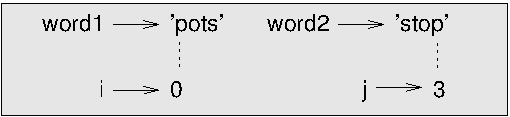
\includegraphics[scale=0.8]{figs/state4.pdf}}
\caption{Διάγραμμα κατάστασης.}
\label{fig.state4}
\end{figure}

Τοποθέτησα τις μεταβλητές μέσα στο πλαίσιο και πρόσθεσα διακεκομμένες λίγο αυθαίρετα για να δείξω ότι οι τιμές του {\tt i} και του {\tt j} δείχνουν χαρακτήρες στην {\tt word1} και στην {\tt word2}.
\\
\begin{exercise}
\label{isreverse}

Ξεκινώντας με αυτό το διάγραμμα, εκτελέστε το πρόγραμμα στο χαρτί αλλάζοντας
τις τιμές των {\tt i} και {\tt j} σε κάθε επανάληψη. Βρείτε και διορθώστε το δεύτερο λάθος σε αυτήν τη συνάρτηση.
\end{exercise}



\section{Ορολογία}

\begin{description}

\item[αντικείμενο:] Κάτι στο οποίο μπορεί να αναφέρεται μία μεταβλητή. Για την ώρα, μπορείτε να χρησιμοποιείτε τους όρους "αντικείμενο" και "τιμή" εναλλάξ.
\index{object}

\item[ακολουθία:] Ένα διατεταγμένο σύνολο τιμών στο οποίο κάθε τιμή προσδιορίζεται από έναν ακέραιο δείκτη.
\index{sequence}

\item[στοιχείο:] Μία από τις τιμές μίας ακολουθίας.
\index{item}

\item[δείκτης:] Μία ακέραια τιμή η οποία χρησιμοποιείται για να επιλέξουμε ένα στοιχείο μίας ακολουθίας, όπως είναι κάποιος χαρακτήρας μιας συμβολοσειράς.
\index{index}

\item[τεμάχιο:] Ένα τμήμα μίας συμβολοσειράς ορισμένο από ένα εύρος δεικτών.
\index{slice}

\item[κενή συμβολοσειρά:] Μία συμβολοσειρά χωρίς χαρακτήρες και με μήκος 0, η οποία αναπαριστάται από δυο κενά εισαγωγικά.
\index{empty string}

\item[αμετάβλητη:] Η ιδιότητα μίας ακολουθίας της οποίας τα στοιχεία δεν μπορούν να αλλάξουν τιμές.
\index{immutability}

\item[διάσχιση:] Η διαδοχική προσπέλαση των στοιχείων μίας συμβολοσειράς με σκοπό την εκτέλεση κάποιας πράξης στο καθένα.
\index{traversal}

\item[αναζήτηση:] Ένα είδος διάσχισης η οποία σταματάει όταν βρει αυτό που ψάχνει.
\index{search pattern}
\index{pattern!search}

\item[μετρητής:] Μία μεταβλητή η οποία χρησιμοποιείται για να μετρήσει κάτι, συνήθως αρχικοποιείται στο μηδέν και μετά προσαυξάνεται.
\index{counter}

\item[μέθοδος:] Μία συνάρτηση η οποία συνδέεται με ένα αντικείμενο και καλείται χρησιμοποιώντας τον συμβολισμό με τελεία.
\index{method}

\item[επίκληση:] Μία δήλωση η οποία καλεί μία μέθοδο.
\index{invocation}

\end{description}


\section{Ασκήσεις}

\begin{exercise}
\index{step size}
\index{slice operator}
\index{operator!slice}

Ένα τεμάχιο συμβολοσειράς μπορεί να πάρει ένα τρίτο όρισμα το οποίο καθορίζει το "μέγεθος βήματος", το οποίο είναι ο αριθμός των κενών μεταξύ των διαδοχικών χαρακτήρων. Ένα μέγεθος βήματος 2 σημαίνει κάθε δεύτερο χαρακτήρα, 3 σημαίνει κάθε τρίτο χαρακτήρα κτλ.


\begin{verbatim}
>>> fruit = 'banana'
>>> fruit[0:5:2]
'bnn'
\end{verbatim}


Ένα μέγεθος βήματος ίσο με -1 διασχίζει τη λέξη προς τα πίσω, δηλαδή το τεμάχιο  \verb"[::-1]" παράγει μία ανεστραμμένη συμβολοσειρά.
\index{palindrome}

Χρησιμοποιήστε αυτήν την ιδιότητα για να γράψετε μία έκδοση μίας γραμμής της  \verb"is_palindrome" της Άσκησης~\ref{palindrome}.
\\
\end{exercise}


\begin{exercise}

Οι ακόλουθες συναρτήσεις προορίζονται για να ελέγχουν εάν μία συμβολοσειρά περιέχει πεζά γράμματα αλλά κάποιες από αυτές είναι λάθος.


\begin{verbatim}
def any_lowercase1(s):
    for c in s:
        if c.islower():
            return True
        else:
            return False

def any_lowercase2(s):
    for c in s:
        if 'c'.islower():
            return 'True'
        else:
            return 'False'

def any_lowercase3(s):
    for c in s:
        flag = c.islower()
    return flag

def any_lowercase4(s):
    flag = False
    for c in s:
        flag = flag or c.islower()
    return flag

def any_lowercase5(s):
    for c in s:
        if not c.islower():
            return False
    return True
\end{verbatim}

Περιγράψτε τι κάνει πραγματικά η κάθε συνάρτηση, θεωρώντας ότι η παράμετρος είναι μία συμβολοσειρά.
\\
\end{exercise}


\begin{exercise}
\index{letter rotation}
\index{rotation, letter}

\label{exrotate}
Η ROT13 είναι μία αδύνατη μορφή κρυπτογράφησης η οποία βασίζεται στην "περιστροφή" (rotating) κάθε γράμματος μίας λέξης κατά 13 θέσεις. Περιστροφή ενός γράμματος σημαίνει μετατόπιση μέσα στο αλφάβητο, επιστρέφοντας μέχρι και στην αρχή εάν είναι απαραίτητο. Έτσι, το 'A' μετατοπισμένο κατά 3 γίνεται 'D' και το 'Z' μετατοπισμένο κατά 1 γίνεται 'A' στο αγγλικό αλφάβητο.

Γράψτε μία συνάρτηση με όνομα \verb"rotate_word" η οποία θα παίρνει μία συμβολοσειρά και έναν ακέραιο σαν παραμέτρους και θα επιστρέφει μία νέα συμβολοσειρά η οποία θα περιέχει τα γράμματα της αρχικής "περιστραμμένα" με βάση το δοθέν ποσό.

Για παράδειγμα, η λέξη "cheer" περιστραμμένη κατά 7 γίνεται "jolly" και η "melon" περιστραμμένη κατά -10 γίνεται "cubed". 

%For example ``sleep''
%rotated by 9 is ``bunny'' and ``latex'' rotated by 7 is ``shale''.

Ενδεχομένως να σας φανούν χρήσιμες οι ενσωματωμένες συναρτήσεις {\tt ord}, η οποία μετατρέπει ένα χαρακτήρα σε έναν μαθηματικό κώδικα, και {\tt chr}, η οποία μετατρέπει αριθμητικούς κώδικες σε χαρακτήρες.

Δυνητικά προσβλητικά αστεία στο διαδίκτυο κρυπτογραφούνται μερικές φορές με  ROT13. Αν δεν προσβάλλεστε εύκολα, βρείτε και αποκρυπτογραφήστε μερικά από αυτά. Λύση: \url{http://thinkpython.com/code/rotate.py}. 

\end{exercise}



\chapter{Μελέτη περίπτωσης: λογοπαίγνια}

\section{Διαβάζοντας λίστες λέξεων}
\label{wordlist}

Για τις ασκήσεις αυτού του κεφαλαίου θα χρειαστούμε μία λίστα αγγλικών λέξεων. Υπάρχουν πολλές τέτοιες λίστες διαθέσιμες στο διαδίκτυο αλλά η καταλληλότερη για το σκοπό μας είναι μία από τις λίστες που συλλέχθηκαν και προσφέρθηκαν ως  "κοινό κτήμα" από τον Γκράντι Γουόρντ ως μέρος του έργου Μόντι (lexicon project Mody βλ. \url{http://wikipedia.org/wiki/Moby_Project}). Αυτή η λίστα αποτελείται από 113.809 "λέξεις σταυρόλεξων", λέξεις δηλαδή οι οποίες θεωρούνται έγκυρες στα σταυρόλεξα και σε άλλα παιχνίδια λέξεων. Στη συλλογή Μόντι, το όνομα του αρχείου είναι {\tt 113809of.fic}, αλλά εσείς μπορείτε να κατεβάσετε ένα αντίγραφο με το απλούστερο όνομα {\tt words.txt} από το σύνδεσμο  \url{http://thinkpython.com/code/words.txt}.
\index{Moby Project}
\index{crosswords}

Αυτό το αρχείο είναι απλό κείμενο (plain text) και μπορείτε να το ανοίξετε με έναν κειμενογράφο, αλλά μπορείτε επίσης να το διαβάσετε και μέσω της Python.  Η ενσωματωμένη συνάρτηση {\tt open} παίρνει το όνομα ενός αρχείου σαν παράμετρο και επιστρέφει ένα αντικείμενο του αρχείου, το οποίο μπορείτε να χρησιμοποιήσετε για να διαβάσετε το αρχείο. 
\index{open function}
\index{function!open}
\index{plain text}
\index{text!plain}
\index{object!file}
\index{file object}

\begin{verbatim}
>>> fin = open('words.txt')
>>> print fin
<open file 'words.txt', mode 'r' at 0xb7f4b380>
\end{verbatim}
%

Το {\tt fin} είναι ένα από τα πιο συνηθισμένα ονόματα για αντικείμενα αρχείων τα οποία χρησιμοποιούνται ως είσοδος. Η λειτουργία \verb"'r'" υποδεικνύει ότι αυτό το αρχείο είναι ανοιχτό για ανάγνωση (εν αντιθέσει με τη \verb"'w'" η οποία είναι για γράψιμο).
\index{readline method}
\index{method!readline}


Τα αντικείμενα αρχείων παρέχουν διάφορες μεθόδους για διάβασμα. Μεταξύ αυτών είναι και η {\tt readline} η οποία διαβάζει χαρακτήρες από ένα αρχείο μέχρι να συναντήσει μία νέα γραμμή και επιστρέφει το αποτέλεσμα σαν συμβολοσειρά:

\begin{verbatim}
>>> fin.readline()
'aa\r\n'
\end{verbatim}
%

Η πρώτη λέξη σε αυτή τη συγκεκριμένη λίστα είναι η "aa", η οποία είναι ένα είδος λάβας. Η ακολουθία \verb"\r\n" αναπαριστά δύο χαρακτήρες λευκού διαστήματος (μία επιστροφή φορέα και μία νέα γραμμή) οι οποίοι χωρίζουν αυτή τη λέξη από την επόμενη.

Το αντικείμενο του αρχείου καταγράφει τη θέση του μέσα στο αρχείο και έτσι αν ξανακαλέσετε την {\tt readline} θα πάρετε την επόμενη λέξη:

\begin{verbatim}
>>> fin.readline()
'aah\r\n'
\end{verbatim}
%

Η επόμενη λέξη είναι η "aah", η οποία θεωρείται απολύτως έγκυρη λέξη και για αυτό σταματήστε να με κοιτάτε έτσι. Αν σας ενοχλούν οι χαρακτήρες λευκού  διαστήματος τότε μπορείτε να τους ξεφορτωθείτε με τη μέθοδο {\tt strip}:
\index{strip method}
\index{method!strip}

\begin{verbatim}
>>> line = fin.readline()
>>> word = line.strip()
>>> print word
aahed
\end{verbatim}
%

Επίσης, μπορείτε να χρησιμοποιήσετε ένα αντικείμενο αρχείου ως μέρος ενός βρόχου {\tt for}. Αυτό το πρόγραμμα διαβάζει το {\tt words.txt} και εμφανίζει όλες τις λέξεις μία μία:
\index{open function}
\index{function!open}

\begin{verbatim}
fin = open('words.txt')
for line in fin:
    word = line.strip()
    print word
    
\end{verbatim}
%

\begin{exercise}

Γράψτε ένα πρόγραμμα το οποίο θα διαβάζει το αρχείο {\tt words.txt} και θα εμφανίζει μόνο τις λέξεις με περισσότερους από 20 χαρακτήρες (οι χαρακτήρες λευκού διαστήματος δεν μετράνε).
\index{whitespace}
\end{exercise}


\section{Ασκήσεις}

Οι λύσεις αυτών των ασκήσεων υπάρχουν στην επόμενη ενότητα. Θα πρέπει τουλάχιστον να προσπαθήσετε να τις λύσετε προτού συνεχίσετε στις λύσεις.
\\

\begin{exercise}

Το 1939 o Ερνέστος Βίνσεντ Ράιτ δημοσίευσε μία νουβέλα 50.000 λέξεων με τίτλο  {\em Gadsby} η οποία δεν περιέχει καθόλου το γράμμα "e". Αυτό δεν είναι και πολύ εύκολο αφού το γράμμα "e" είναι το πιο κοινό γράμμα στα Αγγλικά.

Πράγματι, είναι δύσκολο να δομηθεί μία αυτεξούσια σκέψη χωρίς το πιο κοινό σύμβολο. Είναι πολύ αργό στην αρχή αλλά με σύνεση και πολλές ώρες εξάσκησης μπορείτε σταδιακά να αποκτήσετε ευχέρεια.

Εντάξει, σταματάω τώρα.

Γράψτε μία συνάρτηση με όνομα \verb"has_no_e" η οποία θα επιστρέφει {\tt True}  αν η δοθείσα λέξη δεν περιέχει το γράμμα "e". 

Τροποποιήστε το πρόγραμμα της προηγούμενης ενότητας για να εμφανίζει μόνο τις λέξεις που δεν έχουν καθόλου "e" και υπολογίστε το ποσοστό των λέξεων της λίστας οι οποίες δεν έχουν καθόλου "e".
\\
\end{exercise}
\index{lipogram}


\begin{exercise}

Γράψτε μία συνάρτηση με όνομα {\tt avoids} η οποία θα παίρνει ως πρώτο όρισμα μία λέξη και ως δεύτερο μία συμβολοσειρά από απαγορευμένα γράμματα και θα επιστρέφει {\tt True} αν η λέξη δεν χρησιμοποιεί κανένα από τα αυτά τα γράμματα.

Τροποποιήστε το πρόγραμμά σας ούτως ώστε να ζητάει από το χρήστη να εισάγει μία συμβολοσειρά απαγορευμένων γραμμάτων και μετά να εμφανίζει το πλήθος των λέξεων που δεν περιέχουν κανένα από αυτά. Μπορείτε να βρείτε έναν συνδυασμό από 5 απαγορευμένα γράμματα τα οποία αποκλείουν το μικρότερο πλήθος λέξεων;
\\
\end{exercise}


\begin{exercise}

Γράψτε μία συνάρτηση με όνομα \verb"uses_only" η οποία θα παίρνει σαν πρώτο όρισμα μία λέξη και σαν δεύτερο όρισμα μία συμβολοσειρά γραμμάτων και θα επιστρέφει {\tt True} αν η λέξη περιέχει μόνο τα γράμματα της ακολουθίας. Μπορείτε να κάνετε μία πρόταση χρησιμοποιώντας μόνο τα γράμματα {\tt acefhlo} (εκτός της  "Hoe alfalfa");
\\
\end{exercise}


\begin{exercise}

Γράψτε μία συνάρτηση με όνομα \verb"uses_all" η οποία θα παίρνει μία λέξη και μία συμβολοσειρά από απαιτούμενα γράμματα και θα επιστρέφει {\tt True} αν η λέξη χρησιμοποιεί όλα τα απαιτούμενα γράμματα τουλάχιστον από μία φορά. Πόσες λέξεις υπάρχουν οι οποίες χρησιμοποιούν όλα τα φωνήεντα {\tt aeiou}; 
Και πόσες οι οποίες χρησιμοποιούν όλα τα φωνήεντα {\tt aeiouy};
\\
\end{exercise}


\begin{exercise}

Γράψτε μία συνάρτηση με όνομα \verb"is_abecedarian" η οποία θα επιστρέφει {\tt True} αν τα γράμματα σε μία λέξη εμφανίζονται σε αλφαβητική σειρά (τα διπλά γράμματα δεν πειράζουν). Πόσες "αλφαβητοποιημένες" λέξεις υπάρχουν;
\end{exercise}
\index{abecedarian}



%\begin{exercise}
%\label{palindrome}
%A palindrome is a word that reads the same
%forward and backward, like ``rotator'' and ``noon.''
%Write a boolean function named \verb"is_palindrome" that
%takes a string as a parameter and returns {\tt True} if it is
%a palindrome.

%Modify your program from the previous section to print all
%of the palindromes in the word list and then print the total
%number of palindromes.
%\end{exercise}



\section{Αναζήτηση}
\index{search pattern}
\index{pattern!search}

Όλες οι ασκήσεις της προηγούμενης ενότητας έχουν κάτι κοινό μεταξύ τους. Μπορούν να λυθούν όλες με το πρότυπο αναζήτησης που είδαμε στην Ενότητα~\ref{find}. Το πιο απλό παράδειγμα είναι:

\begin{verbatim}
def has_no_e(word):
    for letter in word:
        if letter == 'e':
            return False
    return True
\end{verbatim}
%

Ο βρόχος {\tt for} διασχίζει τους χαρακτήρες της {\tt word}. Αν βρούμε το γράμμα "e" τότε επιστρέφουμε αμέσως {\tt False}, αλλιώς πρέπει να προχωρήσουμε στο επόμενο γράμμα. Εάν ο βρόχος τελειώσει κανονικά αυτό σημαίνει ότι δεν βρήκαμε κανένα "e" και άρα επιστρέφουμε {\tt True}.
\index{traversal}

% Removing this because we haven't seen the in operator yet.
%\index{in operator}
%\index{operator!in}

%You could write this function more concisely using the {\tt in}
%operator, but I started with this version because it
%demonstrates the logic of the search pattern.
\index{generalization}

Η {\tt avoids} είναι μία πιο γενικευμένη έκδοση της \verb"has_no_e"
αλλά έχει την ίδια δομή:

\begin{verbatim}
def avoids(word, forbidden):
    for letter in word:
        if letter in forbidden:
            return False
    return True
\end{verbatim}
%

Μπορούμε να επιστρέψουμε {\tt False} αμέσως μόλις βρούμε ένα απαγορευμένο γράμμα. Αν φτάσουμε μέχρι το τέρμα του βρόχου τότε επιστρέφουμε {\tt True}.

Η \verb"uses_only" είναι σχεδόν ίδια, με τη μόνη διαφορά ότι η συνθήκη είναι ανεστραμμένη:

\begin{verbatim}
def uses_only(word, available):
    for letter in word:
        if letter not in available:
            return False
    return True
\end{verbatim}
%

Αντί για μία λίστα απαγορευμένων γραμμάτων, έχουμε μία λίστα διαθέσιμων γραμμάτων. Αν βρούμε ένα γράμμα μέσα στη {\tt word} το οποίο δεν υπάρχει στην  {\tt available} επιστρέφουμε {\tt False}.

Η \verb"uses_all" είναι παρόμοια αν εξαιρέσουμε ότι αντιστρέφουμε τον ρόλο της λέξης και της συμβολοσειράς των γραμμάτων:

\begin{verbatim}
def uses_all(word, required):
    for letter in required:
        if letter not in word:
            return False
    return True
\end{verbatim}
%

Αντί ο βρόχος να διασχίζει τα γράμματα της {\tt word}, διασχίζει τα γράμματα που απαιτούνται. Αν κάποιο από τα απαιτούμενα γράμματα δεν εμφανιστεί μέσα στη λέξη τότε επιστρέφουμε {\tt False}.
\index{traversal}


Αν σκεφτόσασταν πραγματικά σαν ένας επιστήμονας της πληροφορικής, τότε θα είχατε αναγνωρίσει ότι η \verb"uses_all" είναι ένα στιγμιότυπο ενός ήδη λυμένου προβλήματος και θα την γράφατε έτσι:

\begin{verbatim}
def uses_all(word, required):
    return uses_only(required, word)
\end{verbatim}
%

Αυτό είναι ένα παράδειγμα μεθόδου ανάπτυξης προγράμματος η οποία ονομάζεται {\bf αναγνώριση προβλήματος} (problem recognition), αυτό σημαίνει ότι αναγνωρίζετε το το πρόβλημα πάνω στο οποίο εργάζεστε ως ένα στιγμιότυπο ενός προβλήματος το οποίο έχει λυθεί ήδη και εφαρμόζετε μία ήδη ανεπτυγμένη λύση.
\index{problem recognition}
\index{development plan!problem recognition}


\section{Βρόχοι επανάληψης με δείκτες}
\index{looping!with indices}
\index{index!looping with}

Στην προηγούμενη ενότητα, έγραψα τις συναρτήσεις με βρόχους {\tt for} γιατί
χρειαζόμουν μόνο τους χαρακτήρες μέσα στις συμβολοσειρές, δεν ήταν ανάγκη να χρησιμοποιήσω δείκτες.

Στην \verb"is_abecedarian" πρέπει να συγκρίνουμε γειτονικά γράμματα, το οποίο είναι λίγο δύσκολο να υλοποιηθεί με έναν βρόχο {\tt for}:

\begin{verbatim}
def is_abecedarian(word):
    previous = word[0]
    for c in word:
        if c < previous:
            return False
        previous = c
    return True
\end{verbatim}


Εναλλακτικά μπορούμε να χρησιμοποιήσουμε αναδρομή:

\begin{verbatim}
def is_abecedarian(word):
    if len(word) <= 1:
        return True
    if word[0] > word[1]:
        return False
    return is_abecedarian(word[1:])
\end{verbatim}


Μία άλλη επιλογή είναι να χρησιμοποιήσουμε ένα βρόχο {\tt while}:

\begin{verbatim}
def is_abecedarian(word):
    i = 0
    while i < len(word)-1:
        if word[i+1] < word[i]:
            return False
        i = i+1
    return True
\end{verbatim}
%

Ο βρόχος αρχίζει με {\tt i=0} και τελειώνει όταν {\tt i=len(word)-1}. 
Σε κάθε επανάληψη, συγκρίνει το $i$οστό χαρακτήρα (τον οποίο μπορείτε να σκέφτεστε σαν τον τρέχον χαρακτήρα) με τον $i+1$οστό (σκεφτείτε τον σαν τον επόμενο).

Αν ο επόμενος χαρακτήρας είναι μικρότερος (αλφαβητικά προηγούμενος) από τον τρέχον, τότε έχουμε ανακαλύψει μία ρήξη στη αλφαβητική φορά και επιστρέφουμε {\tt False}.

Αν ο βρόχος τερματίσει χωρίς να βρούμε κανένα σφάλμα τότε η λέξη έχει περάσει τον έλεγχο. Για να πείσετε τον εαυτό σας ότι ο βρόχος τερματίζει σωστά, σκεφτείτε ένα παράδειγμα όπως το \verb"'flossy'". Το μήκος της λέξης είναι 6, άρα την τελευταία φορά που τρέχει ο βρόχος το {\tt i} είναι 4, το οποίο είναι ο δείκτης του προτελευταίου χαρακτήρα, δηλαδή αυτού που θέλουμε.
\index{palindrome}

Ακολουθεί μία έκδοση της \verb"is_palindrome" (βλ. Άσκηση~\ref{palindrome}) η οποία χρησιμοποιεί δύο δείκτες, ο ένας ξεκινάει από την αρχή και αυξάνεται και ο άλλος ξεκινάει από το τέλος και μειώνεται.


\begin{verbatim}
def is_palindrome(word):
    i = 0
    j = len(word)-1
    
    while i<j:
        if word[i] != word[j]:
            return False
        i = i+1
        j = j-1

    return True
\end{verbatim}


Ή, αν είχατε παρατηρήσει ότι αυτό είναι ένα στιγμιότυπο ενός ήδη λυμένου προβλήματος, ίσως είχατε γράψει:

\begin{verbatim}
def is_palindrome(word):
    return is_reverse(word, word)
\end{verbatim}
\index{problem recognition}
\index{development plan!problem recognition}

Υποθέτοντας ότι έχετε κάνει την Άσκηση~\ref{isreverse}.



\section{Αποσφαλμάτωση}
\index{debugging}
\index{testing!is hard}
\index{program testing}

Η δοκιμή και ο έλεγχος των προγραμμάτων είναι δύσκολες διαδικασίες γενικά.
Οι συναρτήσεις σε αυτό το κεφάλαιο είναι σχετικά εύκολο να δοκιμαστούν γιατί μπορούμε να ελέγξουμε τα αποτελέσματα με το χέρι. Ακόμα κι έτσι όμως, η επιλογή ενός συνόλου λέξεων το οποίο θα καλύπτει όλα τα πιθανά σφάλματα είναι αν όχι αδύνατον, τότε πολύ δύσκολο.

Παίρνοντας σαν παράδειγμα την \verb"has_no_e", υπάρχουν δύο προφανείς περιπτώσεις για να ελέγξουμε: πρώτον οι λέξεις οι οποίες έχουν ένα "e" θα πρέπει να επιστρέφουν {\tt False} και δεύτερον οι λέξεις που δεν έχουν κανένα "e" θα πρέπει να επιστρέφουν {\tt True}. Λογικά, καμία από τις δύο δεν πρέπει να σας δυσκολεύει.

Σε κάθε περίπτωση υπάρχουν μερικές λιγότερο προφανείς υποπεριπτώσεις. Μεταξύ των λέξεων που έχουν ένα "e", θα πρέπει να ελέγξετε λέξεις με ένα "e" στην αρχή, στο τέλος και κάπου στη μέση. Θα πρέπει να ελέγξετε μεγάλες λέξεις, μικρές λέξεις, πολύ μικρές λέξεις ή ακόμα και κενές συμβολοσειρές. Η κενή συμβολοσειρά είναι ένα παράδειγμα {\bf ειδικής περίπτωσης} (special case) η οποία ανήκει στις μη προφανείς περιπτώσεις που συχνά κρύβονται λάθη.
\index{special case}

Εκτός από τις περιπτώσεις που δημιουργείτε εσείς, μπορείτε να δοκιμάσετε το πρόγραμμά σας με μία λίστα λέξεων όπως η {\tt words.txt}. Ελέγχοντας προσεκτικά την έξοδο, ίσως μπορέσετε να βρείτε σφάλματα αλλά να είστε προσεκτικοί γιατί μπορεί να βρείτε κάποιο σφάλμα (λέξεις οι οποίες δεν θα έπρεπε να συμπεριλαμβάνονται και υπάρχουν) αλλά όχι κάποιο άλλο (λέξεις οι οποίες θα έπρεπε να υπάρχουν και δεν συμπεριλαμβάνονται).

Γενικά, οι δοκιμές μπορούν να σας βοηθήσουν να βρείτε σφάλματα αλλά δεν είναι εύκολο να δημιουργήσετε ένα καλό σύνολο περιπτώσεων προς δοκιμή. Ακόμα και αν το καταφέρετε δεν μπορείτε να είστε σίγουροι ότι το πρόγραμμά σας είναι ολόσωστο.
\index{testing!and absence of bugs}

Σύμφωνα με ένα θρυλικό επιστήμονα της πληροφορικής:

\begin{quote}

Η δοκιμή των προγραμμάτων μπορεί να χρησιμοποιηθεί για να αναδείξει την παρουσία σφαλμάτων, αλλά ποτέ για να δείξει την απουσία τους!

--- Edsger W. Dijkstra
\end{quote}
\index{Dijkstra, Edsger}


\section{Ορολογία}

\begin{description}

\item[αντικείμενο αρχείου:] Μία τιμή η οποία αναπαριστά ένα ανοιχτό αρχείο.
\index{file object}
\index{object!file}

\item[αναγνώριση προβλήματος:] Ένας τρόπος επίλυσης ενός προβλήματος εκφράζοντάς το ως ένα στιγμιότυπο ενός ήδη λυμένου προβλήματος.
\index{problem recognition}

\item[ειδική περίπτωση:] Μία άτυπη ή μη προφανής περίπτωση προς δοκιμή (και λιγότερο πιθανό να χειριστεί σωστά).
\index{special case}

\end{description}


\section{Ασκήσεις}

\begin{exercise}
\index{Car Talk}
\index{Puzzler}
\index{double letters}

Η ακόλουθη ερώτηση βασίζεται σε ένα γρίφο ο οποίος μεταδόθηκε στο ραδιοφωνικό σταθμό {\em Car Talk} (\url{http://www.cartalk.com/content/puzzlers}):

\begin{quote}

Βρείτε μία αγγλική λέξη με τρεις συνεχόμενες δυάδες γραμμάτων. Για παράδειγμα, η λέξη  committee: c-o-m-m-i-t-t-e-e  θα ήταν σωστή αν εξαιρέσουμε το "i" στη μέση της και η λέξη Mississippi: M-i-s-s-i-s-s-i-p-p-i  θα ήταν επίσης σωστή αν μπορούσαμε να βγάλουμε το δεύτερο και τρίτο "i". Ωστόσο, υπάρχει τουλάχιστον μία λέξη απ' όσο ξέρω η οποία έχει τρία συνεχόμενα ζευγάρια γραμμάτων. Ενδεχομένως να υπάρχουν ακόμα 500 λέξεις οι οποίες να ικανοποιούν αυτή τη συνθήκη αλλά εγώ μπορώ να σκεφτώ μόνο μία. Ποια είναι η λέξη; 

\end{quote}

Γράψτε ένα πρόγραμμα για να βρείτε αυτή τη λέξη. Λύση :\url{http://thinkpython.com/code/cartalk1.py}.
\\
\end{exercise}

\begin{exercise}
Αυτός είναι ένας άλλος γρίφος από το {\em Car Talk}
(\url{http://www.cartalk.com/content/puzzlers}):
\index{Car Talk}
\index{Puzzler}
\index{odometer}
\index{palindrome}

\begin{quote}
`` Τις προάλλες, καθώς οδηγούσα στον αυτοκινητόδρομο, έτυχε να
προσέξω το οδόμετρο μου, και όπως τα περισσότερα οδόμετρα έτσι και 
αυτό δείχνει με έξι ψηφία μόνο ολόκληρα μίλια. Έτσι, αν για παράδειγμα
το αυτοκίνητό μου είχε 300.000 μίλια, θα έβλεπα 3-0-0-0-0-0.

`` Πρόσεξα λοιπόν κάτι πολύ ενδιαφέρον, τα τελευταία 4 ψηφία ήταν
παλίνδρομα, διαβάζονται δηλαδή το ίδιο προς τα πίσω και προς τα μπρος.
Για παράδειγμα, το 5-4-4-5 είναι ένα παλίνδρομο, έτσι το οδόμετρό
μου μπορεί να έδειχνε 3-1-5-4-4-5.

`` Ένα μίλι αργότερα, τα τελευταία 5 νούμερα ήταν παλίνδρομα. Για παράδειγμα,
μπορεί να ήταν  3-6-5-4-5-6. Ένα μίλι μετά από αυτό, οι τέσσερις μεσαίοι
αριθμοί ήταν παλίνδρομοι και μαντέψτε τι έγινε μετά από ένα ακόμα μίλι. Και τα 6 ψηφία ήταν παλίνδρομα!

`` Και η ερώτηση είναι η εξής, πόσα μίλια είχε το οδόμετρο όταν το κοίταξα πρώτη φορά;''
\end{quote}


Γράψτε ένα πρόγραμμα σε  Python  το οποίο τεστάρει όλους τους εξαψήφιους αριθμούς και εμφανίζει όσους ικανοποιούν αυτές τις απαιτήσεις.
Λύση: \url{http://thinkpython.com/code/cartalk2.py}.
\\
\end{exercise}


\begin{exercise}
Και αυτός είναι ένας ακόμα γρίφος του {\em Car Talk} τον οποίο
μπορείτε να λύσετε με αναζήτηση (\url{http://www.cartalk.com/content/puzzlers}):
\index{Car Talk}
\index{Puzzler}
\index{palindrome}

\begin{quote}
`` Πρόσφατα επισκέφτηκα τη μητέρα μου και καθώς συζητούσαμε,
συνειδητοποιήσαμε ότι αν αντιστρέψουμε τα δύο ψηφία από τα οποία
αποτελείται η ηλικία μου, τότε προκύπτει η δική της ηλικία. Για παράδειγμα,
αν αυτή είναι 73 τότε εγώ είμαι 37. Αναρωτηθήκαμε πόσες φορές έχει συμβεί
αυτό με την πάροδο των χρόνων αλλά αποπροσανατολιστήκαμε από άλλα θέματα
και δεν καταλήξαμε σε κάποια απάντηση. 

`` Όταν γύρισα σπίτι, υπολόγισα ότι τα ψηφία των ηλικιών μας ήταν αντιστρέψιμα
έξι φορές μέχρι τώρα. Υπολόγισα επίσης, ότι αν είμαστε τυχεροί, αυτό θα ξανασυμβεί μία ακόμα φορά μετά από αυτήν και αν είμαστε πολύ τυχεροί, θα μπορούσε να συμβεί 8 φορές συνολικά. Επομένως η ερώτηση είναι: πόσο χρονών είμαι τώρα;''

\end{quote}

Γράψτε ένα πρόγραμμα σε Python το οποίο ψάχνει λύσεις για αυτόν το γρίφο.
Υπόδειξη: ίσως σας φανεί χρήσιμη η μέθοδος {\tt zfill}.

Λύση: \url{http://thinkpython.com/code/cartalk3.py}.
\end{exercise}



\chapter{Λίστες}

\section{Η λίστα είναι μία ακολουθία}
\label{sequence}

Όπως οι συμβολοσειρές, έτσι και οι {\bf λίστες} (lists) είναι ακολουθίες τιμών, με τη διαφορά ότι σε μία συμβολοσειρά οι τιμές είναι χαρακτήρες ενώ σε μία λίστα μπορούν να είναι οποιουδήποτε τύπου. Οι τιμές μίας λίστας ονομάζονται {\bf στοιχεία} (elements/items).
\index{list}
\index{type!list}
\index{element}
\index{sequence}
\index{item}

Υπάρχουν διάφοροι τρόποι για να δημιουργία μίας λίστας, αλλά ο πιο απλός είναι 
περικλείοντας τα στοιχεία μέσα σε αγκύλες (\verb"[" και \verb"]"):

\begin{verbatim}
[10, 20, 30, 40]
['crunchy frog', 'ram bladder', 'lark vomit']
\end{verbatim}
%

Το πρώτο παράδειγμα είναι μία λίστα η οποία αποτελείται από τέσσερις ακέραιους αριθμούς ενώ το δεύτερο είναι μία λίστα τριών συμβολοσειρών. Τα στοιχεία μίας λίστας μπορεί να είναι διαφορετικού τύπου. Η ακόλουθη λίστα περιέχει μία συμβολοσειρά, ένα δεκαδικό, έναν ακέραιο και μία άλλη λίστα:

\begin{verbatim}
['spam', 2.0, 5, [10, 20]]
\end{verbatim}
%

Μία λίστα η οποία βρίσκεται μέσα σε μία άλλη λίστα ονομάζεται {\bf εμφωλευμένη} (nested).
\index{nested list}
\index{list!nested}

Μία λίστα η οποία δεν περιέχει κανένα στοιχείο ονομάζεται κενή λίστα. Η κενή
δημιουργείται με κενές αγκύλες \verb"[]".
\index{empty list}
\index{list!empty}

Όπως θα περιμένατε, μπορείτε να εκχωρήσετε τις τιμές μίας λίστας σε μεταβλητές:

\begin{verbatim}
>>> cheeses = ['Cheddar', 'Edam', 'Gouda']
>>> numbers = [17, 123]
>>> empty = []
>>> print cheeses, numbers, empty
['Cheddar', 'Edam', 'Gouda'] [17, 123] []
\end{verbatim}
%
\index{assignment}


\section{Οι λίστες είναι μεταβλητές}
\label{mutable}
\index{list!element}
\index{access}
\index{index}
\index{bracket operator}
\index{operator!bracket}


Η σύνταξη για την πρόσβαση στα στοιχεία μίας λίστας είναι η ίδια με τη σύνταξη για την πρόσβαση στους χαρακτήρες μίας συμβολοσειράς, χρησιμοποιώντας δηλαδή τον τελεστή αγκύλης. Θυμηθείτε ότι οι δείκτες ξεκινάνε από το 0:

\begin{verbatim}
>>> print cheeses[0]
Cheddar
\end{verbatim}
%

Σε αντίθεση με τις συμβολοσειρές, οι λίστες είναι μεταβλητές. Όταν ο τελεστής αγκύλης εμφανίζεται στο αριστερό μέλος μίας εκχώρησης τότε προσδιορίζει το στοιχείο της λίστας στο οποίο θα εκχωρηθεί το δεξιό μέλος.
\index{mutability}

\begin{verbatim}
>>> numbers = [17, 123]
>>> numbers[1] = 5
>>> print numbers
[17, 5]
\end{verbatim}
%

Το στοιχείο της {\tt numbers} με δείκτη 1 το οποίο ήταν 123, τώρα είναι 5.
\index{index!starting at zero}
\index{zero, index starting at}

Μπορείτε να φανταστείτε μία λίστα σαν μία σχέση μεταξύ δεικτών και στοιχείων. Αυτή η σχέση ονομάζεται {\bf αντιστοίχιση} (mapping). Κάθε δείκτης δηλαδή, αντιστοιχεί σε ένα από τα στοιχεία. Η Εικόνα~\ref{fig.liststate} δείχνει το διάγραμμα κατάστασης για τις {\tt cheeses}, {\tt numbers} και {\tt empty}:
\index{state diagram}
\index{diagram!state}
\index{mapping}

\begin{figure}
\centerline
{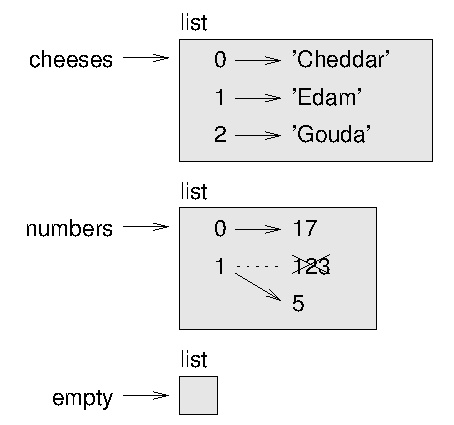
\includegraphics[scale=0.8]{figs/liststate.pdf}}
\caption{Διάγραμμα κατάστασης.}
\label{fig.liststate}
\end{figure}


Οι λίστες αναπαριστώνται από κουτιά με τη λέξη "list" εξωτερικά και
τα στοιχεία της λίστας εντός. Η {\tt cheeses} αναφέρεται σε μία λίστα
τριών στοιχείων με δείκτες 0, 1 και 2. Η {\tt numbers} περιέχει δύο
στοιχεία εκ των οποίων το ένα άλλαξε τιμή (επανεκχωρήθηκε) από 123 σε 5. Η
{\tt empty} αναφέρεται σε μία λίστα χωρίς κανένα στοιχείο.
\index{item assignment}
\index{assignment!item}

Οι δείκτες λιστών δουλεύουν με τον ίδιο τρόπο όπως και οι δείκτες συμβολοσειρών:

\begin{itemize}

\item  Κάθε ακέραια έκφραση μπορεί να χρησιμοποιηθεί σαν δείκτης.

\item  Αν προσπαθήσετε να διαβάσετε ή να γράψετε ένα στοιχείο το οποίο δεν υπάρχει τότε θα πάρετε ένα {\tt IndexError}.
\index{exception!IndexError}
\index{IndexError}

\item  Αν ένας δείκτης έχει αρνητική τιμή τότε μετράει προς τα πίσω από το τέλος της λίστας.

\end{itemize}
\index{list!index}

\index{list!membership}
\index{membership!list}
\index{in operator}
\index{operator!in}


Στις λίστες δουλεύει επίσης και ο τελεστής {\tt in}:

\begin{verbatim}
>>> cheeses = ['Cheddar', 'Edam', 'Gouda']
>>> 'Edam' in cheeses
True
>>> 'Brie' in cheeses
False
\end{verbatim}



\section{Διασχίζοντας μία λίστα}
\index{list!traversal}
\index{traversal!list}
\index{for loop}
\index{loop!for}
\index{statement!for}

Ο πιο συνηθισμένος τρόπος διάσχισης των στοιχείων μίας λίστας είναι
με ένα βρόχο {\tt for}. Η σύνταξη είναι ίδια με τη διάσχιση συμβολοσειρών:

\begin{verbatim}
for cheese in cheeses:
    print cheese
\end{verbatim}
%

Αυτό δουλεύει μια χαρά αν θέλετε μόνο να διαβάσετε τα στοιχεία μίας λίστας. Αν όμως θέλετε να γράψετε ή να ενημερώσετε στοιχεία τότε χρειάζεστε δείκτες. Αυτό
γίνεται, συνήθως, συνδυάζοντας τις συναρτήσεις {\tt range} και {\tt len}:
\index{looping!with indices}
\index{index!looping with}

\begin{verbatim}
for i in range(len(numbers)):
    numbers[i] = numbers[i] * 2
\end{verbatim}
%

Αυτός ο βρόχος διασχίζει τη λίστα και ενημερώνει κάθε στοιχείο. Η {\tt len} 
επιστρέφει το πλήθος των στοιχείων της λίστας και η {\tt range} επιστρέφει μία
λίστα δεικτών από το 0 έως το $n-1$, όπου $n$ το μήκος της λίστας. Σε κάθε επανάληψη η {\tt i} παίρνει το δείκτη του επόμενου στοιχείου και χρησιμοποιείται από τη δήλωση εκχώρησης μέσα στο σώμα για να διαβάσει τη παλιά τιμή του στοιχείου και να εκχωρήσει την νέα.
\index{item update}
\index{update!item}

Ένας βρόχος {\tt for} επί μίας κενής λίστας δεν εκτελεί ποτέ το σώμα του:

\begin{verbatim}
for x in []:
    print 'This never happens.'
\end{verbatim}
%

Παρόλο που μία λίστα μπορεί να περιέχει μία άλλη λίστα, η εμφωλευένη λίστα δεν παύει να είναι ένα στοιχείο από μόνη της. Άρα, το μήκος της ακόλουθης λίστας είναι τέσσερα:
\index{nested list}
\index{list!nested}

\begin{verbatim}
['spam', 1, ['Brie', 'Roquefort', 'Pol le Veq'], [1, 2, 3]]
\end{verbatim}



\section{Πράξεις με λίστες}
\index{list!operation}

Ο τελεστής {\tt +} συνενώνει λίστες:
\index{concatenation!list}
\index{list!concatenation}

\begin{verbatim}
>>> a = [1, 2, 3]
>>> b = [4, 5, 6]
>>> c = a + b
>>> print c
[1, 2, 3, 4, 5, 6]
\end{verbatim}
%

Παρομοίως, ο τελεστής {\tt *} επαναλαμβάνει μία λίστα δοθέντος ενός αριθμού επανάληψης:
\index{repetition!list}
\index{list!repetition}

\begin{verbatim}
>>> [0] * 4
[0, 0, 0, 0]
>>> [1, 2, 3] * 3
[1, 2, 3, 1, 2, 3, 1, 2, 3]
\end{verbatim}
%

Το πρώτο παράδειγμα επαναλαμβάνει την {\tt [0]} τέσσερις φορές και το δεύτερο επαναλαμβάνει τη λίστα {\tt [1, 2, 3]} τρεις φορές.



\section{Λίστες και τεμάχια}
\index{slice operator}
\index{operator!slice}
\index{index!slice}
\index{list!slice}
\index{slice!list}

Ο τελεστής τεμαχισμού δουλεύει επίσης με τις λίστες:

\begin{verbatim}
>>> t = ['a', 'b', 'c', 'd', 'e', 'f']
>>> t[1:3]
['b', 'c']
>>> t[:4]
['a', 'b', 'c', 'd']
>>> t[3:]
['d', 'e', 'f']
\end{verbatim}
%

Αν παραλείψετε τον πρώτο δείκτη τότε το τεμάχιο θα ξεκινήσει από την αρχή.
Αν παραλείψετε το δεύτερο τότε το τεμάχιο θα φτάσει μέχρι το τέλος. Επομένως, αν παραλείψετε και τους δύο το τεμάχιο θα είναι ένα αντίγραφο ολόκληρης της λίστας.
\index{list!copy}
\index{slice!copy}
\index{copy!slice}

\begin{verbatim}
>>> t[:]
['a', 'b', 'c', 'd', 'e', 'f']
\end{verbatim}
%

Από τη στιγμή που οι λίστες είναι μεταβλητές, είναι συχνά χρήσιμο να κρατάτε ένα αντίγραφο πριν περιστρέψετε, ακρωτηριάσετε ή εφαρμόσετε κάποια συνάρτηση σε μία λίστα.
\index{mutability}

Ένας τελεστής τεμάχιο στο αριστερό μέλος μίας εκχώρησης μπορεί να ενημερώσει πολλαπλά στοιχεία:
\index{slice!update}
\index{update!slice}

\begin{verbatim}
>>> t = ['a', 'b', 'c', 'd', 'e', 'f']
>>> t[1:3] = ['x', 'y']
>>> print t
['a', 'x', 'y', 'd', 'e', 'f']
\end{verbatim}
%

% You can add elements to a list by squeezing them into an empty
% slice:

% % \begin{verbatim}
% >>> t = ['a', 'd', 'e', 'f']
% >>> t[1:1] = ['b', 'c']
% >>> print t
% ['a', 'b', 'c', 'd', 'e', 'f']
% \end{verbatim}
% \afterverb
%
% And you can remove elements from a list by assigning the empty list to
% them:

% % \begin{verbatim}
% >>> t = ['a', 'b', 'c', 'd', 'e', 'f']
% >>> t[1:3] = []
% >>> print t
% ['a', 'd', 'e', 'f']
% \end{verbatim}
% \afterverb
%
% But both of those operations can be expressed more clearly
% with list methods.



\section{Μέθοδοι λιστών}
\index{list!method}
\index{method, list}

Η Python παρέχει διάφορες μεθόδους οι οποίες εφαρμόζονται πάνω σε λίστες.
Για παράδειγμα, η {\tt append} προσθέτει ένα νέο στοιχείο στο τέλος μίας λίστας:
\index{append method}
\index{method!append}

\begin{verbatim}
>>> t = ['a', 'b', 'c']
>>> t.append('d')
>>> print t
['a', 'b', 'c', 'd']
\end{verbatim}
%

Η {\tt extend} παίρνει μία λίστα σαν όρισμα και προσαρτά όλα τα στοιχεία της:
\index{extend method}
\index{method!extend}

\begin{verbatim}
>>> t1 = ['a', 'b', 'c']
>>> t2 = ['d', 'e']
>>> t1.extend(t2)
>>> print t1
['a', 'b', 'c', 'd', 'e']
\end{verbatim}
%

Αυτό το παράδειγμα αφήνει ανεπηρέαστη την  {\tt t2}. 

Η {\tt sort} ταξινομεί τα στοιχεία της λίστας από το χαμηλότερο προς το υψηλότερο (αύξουσα σειρά):
\index{sort method}
\index{method!sort}

\begin{verbatim}
>>> t = ['d', 'c', 'e', 'b', 'a']
>>> t.sort()
>>> print t
['a', 'b', 'c', 'd', 'e']
\end{verbatim}
%

Όλες οι μέθοδοι των λιστών είναι κενές (void), τροποποιούν δηλαδή τη λίστα στην οποία εφαρμόζονται και επιστρέφουν {\tt None}. Αν γράψετε, κατά λάθος, {\tt t = t.sort()} τότε θα απογοητευτείτε από το αποτέλεσμα.
\index{void method}
\index{method!void}
\index{None special value}
\index{special value!None}


\section{Map, filter και reduce}

Για να προσθέσετε τους αριθμούς μίας λίστας μπορείτε να χρησιμοποιήσετε ένα βρόχο σαν αυτόν:


% see add.py

\begin{verbatim}
def add_all(t):
    total = 0
    for x in t:
        total += x
    return total
\end{verbatim}
%

Η {\tt total} αρχικοποιείται στο 0 και σε κάθε επανάληψη το {\tt x} παίρνει ένα στοιχείο της λίστας. Ο τελεστής {\tt +=} είναι ένας εύκολος τρόπος για να ενημερώσουμε μία μεταβλητή. Αυτή η {\bf δήλωση εκχώρησης προσαύξησης} (augmented assignment statement):
\index{update operator}
\index{operator!update}
\index{assignment!augmented}
\index{augmented assignment}

\begin{verbatim}
    total += x
\end{verbatim}
%

είναι ισοδύναμη με την:

\begin{verbatim}
    total = total + x
\end{verbatim}
%

Όσο εκτελείται ο βρόχος, η {\tt total} συσσωρεύει το άθροισμα των στοιχείων.
Μία μεταβλητή που χρησιμοποιείται κατ' αυτόν τον τρόπο ονομάζεται {\bf συσσωρευτής} (accumulator) ή {\bf αθροιστής}.
\index{accumulator!sum}

Η άθροιση των στοιχείων μίας λίστας αποτελεί μία τόσο κοινή διαδικασία που η Python την παρέχει σαν ενσωματωμένη συνάρτηση, την {\tt sum}:

\begin{verbatim}
>>> t = [1, 2, 3]
>>> sum(t)
6
\end{verbatim}
%

Μία τέτοια διαδικασία, η οποία συνενώνει μία ακολουθία στοιχείων σε μία ενιαία τιμή, ονομάζεται πολλές φορές {\bf μείωση} (reduce).
\\
\index{reduce pattern}
\index{pattern!reduce}
\index{traversal}


\begin{exercise}

Γράψτε μία συνάρτηση με όνομα \verb"nested_sum" η οποία θα παίρνει μία λίστα από άλλες εμφωλευμένες λίστες ακεραίων, θα αθροίζει τα στοιχεία από όλες τις εμφωλευμένες λίστες και θα επιστρέφει το άθροισμα.
\end{exercise}

Μερικές φορές, θα θέλετε να διασχίσετε μία λίστα καθώς οικοδομείτε μία άλλη. Για παράδειγμα, η ακόλουθη συνάρτηση παίρνει μία λίστα συμβολοσειρών και επιστρέφει μία νέα λίστα η οποία περιέχει τις συμβολοσειρές κεφαλαιοποιημένες (με κεφαλαίο δηλαδή το πρώτο γράμμα):

\begin{verbatim}
def capitalize_all(t):
    res = []
    for s in t:
        res.append(s.capitalize())
    return res
\end{verbatim}
%

Η {\tt res} αρχικοποιείται με μία κενή λίστα και σε κάθε επανάληψη προσαρτούμε το επόμενο στοιχείο. Επομένως, η {\tt res} είναι ένα ακόμα είδος συσσωρευτή.
\index{accumulator!list}

Μερικές φορές, μία διαδικασία όπως η \verb"capitalize_all" ονομάζεται {\bf map} 
επειδή αντιστοιχίζει μία συνάρτηση (σε αυτήν την περίπτωση την μέθοδο {\tt capitalize}) σε κάθε ένα από τα στοιχεία μίας ακολουθίας.
\\
\index{map pattern}
\index{pattern!map}
\index{filter pattern}
\index{pattern!filter}

\begin{exercise}

Χρησιμοποιήστε την \verb"capitalize_all" για να γράψετε μία συνάρτηση με όνομα  \verb"capitalize_nested" η οποία θα παίρνει μία λίστα από εμφωλευμένες λίστες συμβολοσειρών και θα επιστρέφει μία νέα λίστα με όλες τις συμβολοσειρές κεφαλαιοποιημένες.
\end{exercise}

Μία ακόμη συνηθισμένη διαδικασία είναι η επιλογή κάποιων στοιχείων μίας λίστας και η επιστροφή μίας υπολίστας (sublist). Για παράδειγμα, η παρακάτω συνάρτηση παίρνει μία λίστα συμβολοσειρών και επιστρέφει μία λίστα η οποία περιέχει
μόνο τις κεφαλαίες συμβολοσειρές (αυτές δηλαδή που έχουν όλα τα γράμματα κεφαλαία):

\begin{verbatim}
def only_upper(t):
    res = []
    for s in t:
        if s.isupper():
            res.append(s)
    return res
\end{verbatim}
%

Η {\tt isupper} είναι μία μέθοδος συμβολοσειρών η οποία επιστρέφει {\tt True}
αν η συμβολοσειρά περιέχει μόνο κεφαλαία γράμματα.

Μία διαδικασία όπως η \verb"only_upper" ονομάζεται {\bf φίλτρο} (filter) γιατί επιλέγει κάποια από τα στοιχεία και αγνοεί τα υπόλοιπα.

Οι πιο συνηθισμένες πράξεις στις λίστες μπορούν να εκφραστούν σαν ένας συνδυασμός από map, filter και reduce. Επειδή αυτές η διαδικασίες είναι τόσο κοινές, η  Python παρέχει κάποια χαρακτηριστικά για να τις υποστηρίξει, συμπεριλαμβανομένων της ενσωματωμένης συνάρτησης {\tt map} και ενός τελεστή που ονομάζεται "κατανόηση λίστας".
\\
\index{list!comprehension}


\begin{exercise}
\label{cumulative}
\index{cumulative sum}

Γράψτε μία συνάρτηση η οποία θα παίρνει μία λίστα από αριθμούς και θα επιστρέφει το συσσωρευτικό άθροισμά τους, το οποίο θα είναι μία νέα λίστα όπου το $i$οστό στοιχείο θα είναι το άθροισμα των πρώτων $i+1$ στοιχείων της αρχικής λίστας. Για παράδειγμα, το άθροισμα των στοιχείων της {\tt [1, 2, 3]} θα είναι {\tt [1, 3, 6]}.
\end{exercise}


\section{Διαγραφή στοιχείων}
\index{element deletion}
\index{deletion, element of list}

Υπάρχουν διάφοροι τρόποι για να διαγράψετε στοιχεία από μία λίστα. Αν γνωρίζετε το δείκτη του στοιχείου που θέλετε τότε μπορείτε να χρησιμοποιήσετε την {\tt pop}:
\index{pop method}
\index{method!pop}

\begin{verbatim}
>>> t = ['a', 'b', 'c']
>>> x = t.pop(1)
>>> print t
['a', 'c']
>>> print x
b
\end{verbatim}
%

Η {\tt pop} τροποποιεί τη λίστα και επιστρέφει το στοιχείο που αφαιρέθηκε.
Αν δεν της δώσετε κάποιο δείκτη, διαγράφει και επιστρέφει το τελευταίο στοιχείο της λίστας.

Αν δεν χρειάζεστε τη διαγραμμένη τιμή, μπορείτε να χρησιμοποιήσετε τον τελεστή {\tt del}:
\index{del operator}
\index{operator!del}

\begin{verbatim}
>>> t = ['a', 'b', 'c']
>>> del t[1]
>>> print t
['a', 'c']
\end{verbatim}
%

Αν γνωρίζετε το στοιχείο που θέλετε να αφαιρέσετε (αλλά όχι το δείκτη), μπορείτε να χρησιμοποιήσετε την {\tt remove}:
\index{remove method}
\index{method!remove}

\begin{verbatim}
>>> t = ['a', 'b', 'c']
>>> t.remove('b')
>>> print t
['a', 'c']
\end{verbatim}
%

Η επιστρεφόμενη τιμή από τη {\tt remove} είναι {\tt None}.
\index{None special value}
\index{special value!None}

Για να αφαιρέσετε περισσότερα από ένα στοιχεία, μπορείτε να χρησιμοποιήσετε την  {\tt del} με δείκτη ένα τεμάχιο:

\begin{verbatim}
>>> t = ['a', 'b', 'c', 'd', 'e', 'f']
>>> del t[1:5]
>>> print t
['a', 'f']
\end{verbatim}
%

Όπως συνήθως, το τεμάχιο επιλέγει όλα τα στοιχεία μέχρι, αλλά μη συμπεριλαμβανομένου, τον δεύτερο δείκτη.
\\
\begin{exercise}

Γράψτε μία συνάρτηση με όνομα \verb"middle" η οποία θα παίρνει μία λίστα και θα επιστρέφει μία νέα λίστα η οποία θα περιέχει όλα τα στοιχεία της πρώτης, εκτός από το πρώτο και το τελευταίο. Έτσι, δοθείσας της \verb"middle([1,2,3,4])" θα πρέπει να επιστρέψει \verb"[2,3]".
\\
\end{exercise}

\begin{exercise}

Γράψτε μία συνάρτηση με όνομα \verb"chop" η οποία θα παίρνει μία λίστα, θα την τροποποιεί αφαιρώντας το πρώτο και το τελευταίο στοιχείο και θα επιστρέφει  {\tt None}. 
\end{exercise}


\section{Λίστες και συμβολοσειρές}
\index{list}
\index{string}
\index{sequence}

Μία συμβολοσειρά είναι μία ακολουθία χαρακτήρων και μία λίστα είναι μία ακολουθία τιμών, αλλά μία λίστα χαρακτήρων δεν είναι το ίδιο με μία συμβολοσειρά. Για να μετατρέψετε μία συμβολοσειρά σε μία λίστα χαρακτήρων μπορείτε να χρησιμοποιήσετε την {\tt list}:
\index{list!function}
\index{function!list}

\begin{verbatim}
>>> s = 'spam'
>>> t = list(s)
>>> print t
['s', 'p', 'a', 'm']
\end{verbatim}
%

Επειδή το {\tt list} είναι το όνομα μίας ενσωματωμένης συνάρτησης, θα πρέπει να αποφεύγετε να το χρησιμοποιείτε σαν όνομα μεταβλητής. Εγώ αποφεύγω επίσης την χρήση του {\tt l} επειδή μοιάζει πάρα πολύ με το {\tt 1}. Γι' αυτό χρησιμοποιώ το {\tt t}.

Η συνάρτηση {\tt list} σπάει μία συμβολοσειρά σε μεμονωμένα γράμματα. Αν θέλετε να σπάσετε μία συμβολοσειρά σε λέξεις, μπορείτε να χρησιμοποιήσετε τη μέθοδο {\tt split}:
\index{split method}
\index{method!split}

\begin{verbatim}
>>> s = 'pining for the fjords'
>>> t = s.split()
>>> print t
['pining', 'for', 'the', 'fjords']
\end{verbatim}
%
Ένα προαιρετικό όρισμα με όνομα {\bf διαχωριστής} (delimiter) καθορίζει ποιοι χαρακτήρες θα χρησιμοποιηθούν σαν όρια των λέξεων. Το ακόλουθο παράδειγμα χρησιμοποιεί για διαχωριστή μία παύλα:
\index{optional argument}
\index{argument!optional}
\index{delimiter}

\begin{verbatim}
>>> s = 'spam-spam-spam'
>>> delimiter = '-'
>>> s.split(delimiter)
['spam', 'spam', 'spam']
\end{verbatim}
%

Η {\tt join} είναι το αντίστροφο της {\tt split}. Παίρνει μία λίστα συμβολοσειρών και συνενώνει τα στοιχεία. Αφού η {\tt join} είναι μία μέθοδος συμβολοσειρών, θα πρέπει να την επικαλεστείτε στο διαχωριστή και να περάσετε τη λίστα σαν παράμετρο:
\index{join method}
\index{method!join}
\index{concatenation}

\begin{verbatim}
>>> t = ['pining', 'for', 'the', 'fjords']
>>> delimiter = ' '
>>> delimiter.join(t)
'pining for the fjords'
\end{verbatim}
%
Σε αυτήν την περίπτωση ο διαχωριστής είναι ο χαρακτήρας κενού διαστήματος και άρα η {\tt join} βάζει ένα κενό ανάμεσα στις λέξεις. Για συνενώσετε συμβολοσειρές χωρίς κενά μπορείτε να χρησιμοποιήσετε σαν διαχωριστή την κενή συμβολοσειρά (\verb"''") 
\index{empty string}
\index{string!empty}


\section{Αντικείμενα και τιμές}
\index{object}
\index{value}

Αν εκτελέσουμε αυτές τις δηλώσεις εκχώρησης:

\begin{verbatim}
a = 'banana'
b = 'banana'
\end{verbatim}
%

Ξέρουμε ότι τόσο η {\tt a} όσο και η {\tt b} αναφέρονται σε μία συμβολοσειρά αλλά δεν εάν αναφέρονται στην ίδια συμβολοσειρά. Υπάρχουν δύο πιθανές καταστάσεις οι οποίες φαίνονται στην Εικόνα~\ref{fig.list1}.
\index{aliasing}

\begin{figure}
\centerline
{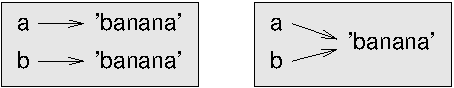
\includegraphics[scale=0.8]{figs/list1.pdf}}
 \caption{Διάγραμμα κατάστασης.} 
\label{fig.list1}
\end{figure}


Στη μία περίπτωση η {\tt a} και {\tt b} αναφέρονται σε δύο διαφορετικά αντικείμενα τα οποία έχουν την ίδια τιμή, ενώ στη δεύτερη περίπτωση αναφέρονται στο ίδιο αντικείμενο.
\index{is operator}
\index{operator!is}

Για να ελέγξετε εάν δύο μεταβλητές αναφέρονται στο ίδιο αντικείμενο, μπορείτε να χρησιμοποιήσετε τον τελεστή {\tt is}.

\begin{verbatim}
>>> a = 'banana'
>>> b = 'banana'
>>> a is b
True
\end{verbatim}
%

Σε αυτό το παράδειγμα η  Python  δημιούργησε μόνο ένα αντικείμενο συμβολοσειράς στο οποίο αναφέρεται και η {\tt a} και η {\tt b}.

Αν δημιουργείτε όμως δύο λίστες τότε θα έχετε δύο ξεχωριστά αντικείμενα:

\begin{verbatim}
>>> a = [1, 2, 3]
>>> b = [1, 2, 3]
>>> a is b
False
\end{verbatim}
%
Έτσι το διάγραμμα κατάστασης είναι όπως αυτό στην Εικόνα~\ref{fig.list2}.
\index{state diagram}
\index{diagram!state}

\begin{figure}
\centerline
{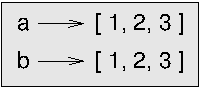
\includegraphics[scale=0.8]{figs/list2.pdf}}
 \caption{Διάγραμμα κατάστασης.} 
\label{fig.list2}
\end{figure}


Σε αυτήν την περίπτωση, θα λέγαμε ότι οι δύο λίστες είναι {\bf ισότιμες} επειδή έχουν τα ίδια στοιχεία, αλλά όχι {\bf ταυτόσημες} αφού είναι δύο διαφορετικά αντικείμενα. Αν δύο αντικείμενα είναι ταυτόσημα τότε είναι και ισότιμα, αλλά αν είναι ισότιμα τότε δεν είναι κατ' ανάγκη και ταυτόσημα.
\index{equivalence}
\index{identity}

Μέχρι τώρα χρησιμοποιούσαμε τους όρους "αντικείμενο" και "τιμή" εναλλάξ, αλλά για να ήμαστε ακριβείς είναι πιο σωστό να πούμε ότι ένα αντικείμενο έχει μία τιμή. Αν εκτελέσετε {\tt [1,2,3]} θα πάρετε ένα αντικείμενο λίστας, η τιμή του οποίου είναι μία ακολουθία ακεραίων. Αν μία λίστα έχει τα ίδια στοιχεία με αυτήν τότε λέμε ότι έχει την ίδια τιμή αλλά δεν είναι το ίδιο αντικείμενο.
\index{object}
\index{value}


\section{Ψευδώνυμα}
\index{aliasing}
\index{reference!aliasing}

Αν μία μεταβλητή {\tt a} αναφέρεται σε ένα αντικείμενο και εσείς την εκχωρήσετε σε μία άλλη μεταβλητή b ({\tt b = a}), τότε και οι δύο μεταβλητές θα αναφέρονται στο ίδιο αντικείμενο:

\begin{verbatim}
>>> a = [1, 2, 3]
>>> b = a
>>> b is a
True
\end{verbatim}
%
 
Το διάγραμμα κατάστασης φαίνεται στην Εικόνα~\ref{fig.list3}.
\index{state diagram}
\index{diagram!state}

\begin{figure}
\centerline
{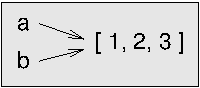
\includegraphics[scale=0.8]{figs/list3.pdf}}
 \caption{Διάγραμμα κατάστασης.} 
\label{fig.list3}
\end{figure}

 
Η σύνδεση μίας μεταβλητής με ένα αντικείμενο ονομάζεται {\bf αναφορά} (reference). Σε αυτό το παράδειγμα, υπάρχουν δύο αναφορές στο ίδιο αντικείμενο.
\index{reference}

Ένα αντικείμενο με περισσότερες από μία αναφορές έχει και περισσότερα από ένα ονόματα, έτσι λέμε ότι το αντικείμενο έχει {\bf ψευδώνυμα} (aliases).
\index{mutability}
 
Αν ένα αντικείμενο με ψευδώνυμο είναι μεταβλητό, οι αλλαγές που γίνονται με το ένα ψευδώνυμο επηρεάζουν και το άλλο:

\begin{verbatim}
>>> b[0] = 17
>>> print a
[17, 2, 3]
\end{verbatim}
%
 
Παρόλο που αυτή η συμπεριφορά μπορεί να φανεί χρήσιμη, είναι επιρρεπής σε λάθη. Γενικά, είναι ασφαλέστερο να αποφεύγετε τα ψευδώνυμα όταν εργάζεστε με αντικείμενα που μπορεί να αλλάξει η τιμή τους (mutable).  
\index{immutability}

Για αμετάβλητα αντικείμενα όπως οι συμβολοσειρές, η εκχώρηση ψευδώνυμων δεν αποτελεί τόσο μεγάλο πρόβλημα. Σε αυτό το παράδειγμα:

\begin{verbatim}
a = 'banana'
b = 'banana'
\end{verbatim}
%

Δεν έχει σχεδόν καμία διαφορά είτε η {\tt a} και {\tt b} αναφέρονται στην ίδια είτε διαφορετική συμβολοσειρά.


\section{Ορίσματα λίστας}
\label{list.arguments}
\index{list!as argument}
\index{argument}
\index{argument!list}
\index{reference}
\index{parameter}

Όταν περνάτε μία λίστα σαν όρισμα σε μία συνάρτηση, η συνάρτηση αποκτά μία αναφορά σε αυτή τη λίστα. Αυτό σημαίνει ότι αν η συνάρτηση τροποποιήσει μία παράμετρο της λίστας τότε ο καλών βλέπει αυτήν την αλλαγή. Για παράδειγμα, η \verb"delete_head" αφαιρεί το πρώτο στοιχείο από μία λίστα:

\begin{verbatim}
def delete_head(t):
    del t[0]
\end{verbatim}
%
 
Εδώ φαίνεται πώς χρησιμοποιείται:	

\begin{verbatim}
>>> letters = ['a', 'b', 'c']
>>> delete_head(letters)
>>> print letters
['b', 'c']
\end{verbatim}
%
 
Η παράμετρος {\tt t} και η μεταβλητή {\tt letters} είναι ψευδώνυμα για το ίδιο αντικείμενο. Το διάγραμμα κατάστασης φαίνεται στην Εικόνα~\ref{fig.stack5}.
\index{stack diagram}
\index{diagram!stack}

\begin{figure}
\centerline
{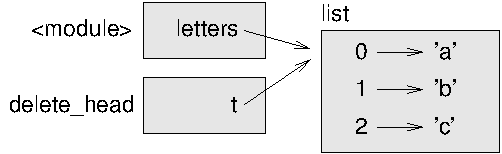
\includegraphics[scale=0.8]{figs/stack5.pdf}}
 \caption{Διάγραμμα κατάστασης.} 
\label{fig.stack5}
\end{figure}


Σχεδίασα τη λίστα ανάμεσα στα δύο πλαίσια γιατί είναι κοινόχρηστη μεταξύ τους.

Είναι σημαντικό να γίνει διάκριση μεταξύ των πράξεων οι οποίες τροποποιούν λίστες και των πράξεων οι οποίες δημιουργούν νέες λίστες. Για παράδειγμα, η μέθοδος {\tt append} τροποποιεί μία λίστα, αλλά ο τελεστής {\tt +} δημιουργεί μία νέα λίστα:
\index{append method}
\index{method!append}
\index{list!concatenation}
\index{concatenation!list}

\begin{verbatim}
>>> t1 = [1, 2]
>>> t2 = t1.append(3)
>>> print t1
[1, 2, 3]
>>> print t2
None

>>> t3 = t1 + [4]
>>> print t3
[1, 2, 3, 4]
\end{verbatim}

 
Αυτή η διαφορά είναι πολύ σημαντική όταν γράφετε συναρτήσεις οι οποίες υποτίθεται ότι τροποποιούν λίστες. Για παράδειγμα, αυτή η συνάρτηση δεν διαγράφει την κεφαλή μίας λίστας:

\begin{verbatim}
def bad_delete_head(t):
    t = t[1:]              # WRONG!
\end{verbatim}

 
Ο τελεστής τεμάχιο δημιουργεί μία νέα λίστα και η εκχώρηση κάνει την {\tt t} να αναφέρεται σε αυτήν την λίστα, αλλά τίποτα από αυτά δεν επηρεάζει τη λίστα που περάστηκε σαν όρισμα.
\index{slice operator}
\index{operator!slice}

Μία εναλλακτική λύση είναι να γράψετε μία συνάρτηση η οποία θα δημιουργεί και θα επιστρέφει μία νέα λίστα. Για παράδειγμα, η {\tt tail} επιστρέφει όλα τα στοιχεία μίας λίστας εκτός από το πρώτο:

\begin{verbatim}
def tail(t):
    return t[1:]
\end{verbatim}
%
 
Αυτή η συνάρτηση αφήνει την αρχική λίστα αμετάβλητη.
Αυτό είναι ένα παράδειγμα χρήσης της:

\begin{verbatim}
>>> letters = ['a', 'b', 'c']
>>> rest = tail(letters)
>>> print rest
['b', 'c']
\end{verbatim}


 
\section{Αποσφαλμάτωση}
\index{debugging}

Η απρόσεκτη χρήση λιστών (και άλλων μεταβλητών αντικειμένων) μπορεί να οδηγήσει σε πολύωρη αποσφαλμάτωση. Αυτές είναι μερικές από τις πιο συνηθισμένες παγίδες και μερικοί τρόποι για να τις αποφεύγετε:

\begin{enumerate}

\item  Να θυμάστε ότι οι περισσότερες μέθοδοι λιστών τροποποιούν το όρισμα και επιστρέφουν {\tt None}, εν αντιθέσει με τις μεθόδους συμβολοσειρών οι οποίες επιστρέφουν μία νέα συμβολοσειρά και αφήνουν την αρχική απείραχτη.
  
Αν έχετε συνηθίσει να γράφετε τέτοιο κώδικα για συμβολοσειρές:  

\begin{verbatim}
word = word.strip()
\end{verbatim}

Τότε ίσως μπείτε στον πειρασμό να γράψετε και τέτοιο κώδικα για λίστες:

\begin{verbatim}
t = t.sort()           # WRONG!
\end{verbatim}
\index{sort method}
\index{method!sort}

Η επόμενη πράξη που θα εκτελέσετε με την {\tt t} πιθανόν να αποτύχει, αφού η {\tt sort} επιστρέφει {\tt None}.

Καλό θα ήταν, προτού χρησιμοποιήσετε μεθόδους και τελεστές στις λίστες, να διαβάσετε την τεκμηρίωση προσεκτικά και να τις δοκιμάσετε σε διαδραστική λειτουργία. Οι μέθοδοι και οι τελεστές που μοιράζονται οι λίστες με άλλες ακολουθίες (όπως οι συμβολοσειρές) τεκμηριώνονται στην διεύθυνση \url{http://docs.python.org/2/library/stdtypes.html#typesseq}. Οι μέθοδοι και οι τελεστές που εφαρμόζονται μόνο σε μεταβλητές ακολουθίες τεκμηριώνονται στη διεύθυνση  \url{http://docs.python.org/2/library/stdtypes.html#typesseq-mutable}.


\item  Επιλέξτε ένα τρόπο γραφής και εμμείνετε σε αυτόν.

Ένα μέρος του προβλήματος με τις λίστες είναι ότι υπάρχουν πολλοί τρόποι για να κάνετε ένα συγκεκριμένο πράγμα. Για παράδειγμα, για να αφαιρέσετε ένα στοιχείο από μία λίστα μπορείτε να χρησιμοποιήσετε την {\tt pop}, την {\tt remove}, την  {\tt del} ή ακόμα και μία εκχώρηση με τεμάχιο.

Για να προσθέσετε ένα στοιχείο, μπορείτε να χρησιμοποιήσετε είτε την μέθοδο {\tt append} είτε τον τελεστή {\tt +}. Υποθέτοντας ότι η {\tt t} είναι μία λίστα και το {\tt x} είναι ένα στοιχείο της λίστας τότε αυτά είναι σωστά:

\begin{verbatim}
t.append(x)
t = t + [x]
\end{verbatim}

Και αυτά είναι λάθος:

\begin{verbatim}
t.append([x])          # WRONG!
t = t.append(x)        # WRONG!
t + [x]                # WRONG!
t = t + x              # WRONG!
\end{verbatim}

 
Δοκιμάστε κάθε ένα από αυτά τα παραδείγματα στη διαδραστική λειτουργία για να σιγουρευτείτε ότι καταλαβαίνετε τι κάνουν. Παρατηρήστε ότι μόνο το τελευταίο προκαλεί σφάλμα χρόνου εκτέλεσης, ενώ τα άλλα τρία είναι έγκυρα αλλά δεν κάνουν αυτό που θα έπρεπε.


\item  Φτιάξτε αντίγραφα για να αποφεύγετε τα ψευδώνυμα.
\index{aliasing!copying to avoid}
\index{copy!to avoid aliasing}

Εάν θέλετε να χρησιμοποιήσετε μία μέθοδο όπως η {\tt sort}, η οποία τροποποιεί το όρισμα, αλλά ταυτόχρονα θέλετε να κρατήσετε και την αρχική λίστα απείραχτη τότε μπορείτε να κάνετε ένα αντίγραφο.
 

\begin{verbatim}
orig = t[:]
t.sort()
\end{verbatim}

 
Σε αυτό το παράδειγμα θα μπορούσατε επίσης να χρησιμοποιήσετε την ενσωματωμένη συνάρτηση {\tt sorted}, η οποία επιστρέφει μία νέα ταξινομημένη λίστα χωρίς να πειράζει την αρχική. Αλλά σε αυτήν την περίπτωση θα πρέπει να αποφύγετε τη χρήση της λέξης {\tt sorted} σαν όνομα μεταβλητής!

\end{enumerate}


 
\section{Ορολογία}

\begin{description}

\item[λίστα:] Μία ακολουθία τιμών.
\index{list}

\item[στοιχείο:] Μία από τις τιμές μίας λίστας (ή κάποιας άλλης ακολουθίας).
\index{element}

\item[δείκτης:] Μία ακέραια τιμή η οποία δείχνει κάποιο στοιχείο μέσα σε μία λίστα.
\index{index}

\item[εμφωλευμένη λίστα:] Μία λίστα η οποία είναι στοιχείο μίας άλλης λίστας.
\index{nested list}

\item[διάσχιση λίστας:] Η διαδοχική προσπέλαση κάθε στοιχείου μίας λίστας.
\index{list!traversal}

\item[αντιστοίχιση:] Μία σχέση στην οποία κάθε στοιχείο ενός συνόλου αντιστοιχεί σε ένα στοιχείο 
κάποιου άλλου συνόλου. Για παράδειγμα, μία λίστα είναι μία αντιστοίχιση από δείκτες σε στοιχεία.
\index{mapping}

\item[συσσωρευτής:] Μία μεταβλητή η οποία χρησιμοποιείται σε ένα βρόχο για να αθροίζει ή να συσσωρεύει ένα αποτέλεσμα. Είναι γνωστή και ως αθροιστής.
\index{accumulator}

\item[εκχώρηση προσαύξησης:] Μία δήλωση η οποία ενημερώνει την τιμή μίας μεταβλητής χρησιμοποιώντας ένα τελεστή όπως ο \verb"+=".
\index{assignment!augmented}
\index{augmented assignment}
\index{traversal}

\item[reduce:] Ένα πρότυπο επεξεργασίας το οποίο διασχίζει μία ακολουθία και συσσωρεύει τα στοιχεία της σε ένα μεμονωμένο αποτέλεσμα.
\index{reduce pattern}
\index{pattern!reduce}
 
\item[map:] Ένα πρότυπο επεξεργασίας το οποίο διασχίζει μία ακολουθία και εκτελεί μία συγκεκριμένη πράξη σε κάθε ένα στοιχείο.
\index{map pattern}
\index{pattern!map}

\item[filter:] Ένα πρότυπο επεξεργασίας το οποίο διασχίζει μία λίστα και επιλέγει τα στοιχεία τα οποία ικανοποιούν ένα συγκεκριμένο κριτήριο.
\index{filter pattern}
\index{pattern!filter}

\item[αντικείμενο:] Κάτι στο οποίο μπορεί να αναφερθεί μία μεταβλητή. Ένα αντικείμενο έχει τύπο και τιμή.
\index{object}

\item[ισότιμα:] Έχουν την ίδια τιμή.
\index{equivalent}

\item[ταυτόσημα:] Να είναι το ίδιο αντικείμενο (συνεπάγεται και ισοτιμία).
\index{identical}

\item[αναφορά:] Η σχέση μεταξύ μίας μεταβλητής και της τιμής της.
\index{reference}

\item[ψευδώνυμα:] Όταν δύο ή περισσότερες μεταβλητές αναφέρονται στο ίδιο αντικείμενο.
\index{aliasing}

\item[διαχωριστής:] Ένας χαρακτήρας ή μία συμβολοσειρά που χρησιμοποιείται για να υποδείξει που πρέπει να χωριστεί μία συμβολοσειρά.
\index{delimiter}

\end{description}


\section{Ασκήσεις}

\begin{exercise}
Γράψτε μία συνάρτηση με όνομα \verb"is_sorted" η οποία θα παίρνει μία λίστα σαν παράμετρο και θα επιστρέφει {\tt True} αν η λίστα είναι ταξινομημένη σε αύξουσα σειρά και {\tt False} αλλιώς. Μπορείτε να θεωρήσετε (ως προϋπόθεση) ότι τα στοιχεία της λίστας μπορούν να συγκριθούν μεταξύ τους με τη χρήση των σχεσιακών τελεστών {\tt <}, {\tt >}, κτλ.
\index{precondition}

Για παράδειγμα, η \verb"is_sorted([1,2,2])" θα πρέπει να επιστρέψει {\tt True}  και η \verb"is_sorted(['b','a'])" θα πρέπει να επιστρέψει {\tt False}.
\\
\end{exercise}
 

\begin{exercise}
\label{anagram}
\index{anagram}

Δύο λέξεις είναι αναγραμματισμοί αν με αναδιάταξη των γραμμάτων της μίας μπορούμε να συλλαβίσουμε την άλλη. Γράψτε μία συνάρτηση με όνομα \verb"is_anagram" η οποία θα παίρνει δύο λέξεις και θα επιστρέφει 
{\tt True} αν είναι αναγραμματισμοί.
\\
\end{exercise}


\begin{exercise}
\label{duplicate}

Το (λεγόμενο) Παράδοξο των Γενεθλίων:

\begin{enumerate}

\item  Γράψτε μία συνάρτηση με όνομα \verb"has_duplicates" η οποία θα παίρνει μία λίστα και θα επιστρέφει {\tt True} αν υπάρχει έστω και ένα στοιχείο το οποίο εμφανίζεται περισσότερες από μία φορές. Δεν πρέπει να τροποποιεί την αρχική αρχική λίστα.
\index{birthday paradox}
\index{duplicate}

\item  Έστω ότι υπάρχουν 23 φοιτητές στην τάξη σας, ποιες είναι οι πιθανότητες δύο από εσάς να έχουν την ίδια ηλικία; Μπορείτε να υπολογίσετε αυτήν την πιθανότητα μέσω της παραγωγής τυχαίων δειγμάτων για 23 ημέρες γενεθλίων και ελέγχοντας ποιες από αυτές ταιριάζουν. Σημείωση: μπορείτε να παράγετε τυχαίες ημέρες γενεθλίων με τη συνάρτηση {\tt randint} του αρθρώματος {\tt random}.
\index{random module}
\index{module!random}
\index{randint function}
\index{function!randint}

\end{enumerate}

Μπορείτε να διαβάσετε για αυτό το πρόβλημα στη διεύθυνση \url{http://en.wikipedia.org/wiki/Birthday_paradox}, και μπορείτε να κατεβάσετε τη δική μου λύση από εδώ: \url{http://thinkpython.com/code/birthday.py}.
\\
\end{exercise}


\begin{exercise}
\index{duplicate}
\index{uniqueness}

Γράψτε μία συνάρτηση με όνομα \verb"remove_duplicates" η οποία θα παίρνει μία λίστα και θα επιστρέφει μία νέα λίστα η οποία θα περιέχει μόνο τα μοναδικά στοιχεία από την αρχική. Σημείωση: Δεν είναι απαραίτητο να είναι με την ίδια σειρά.
\\
\end{exercise}


\begin{exercise}
\index{append method}
\index{method append}
\index{list!concatenation}
\index{concatenation!list}

Γράψτε μία συνάρτηση η οποία θα διαβάζει το αρχείο {\tt words.txt} και θα κατασκευάζει μία λίστα με ένα στοιχείο ανά λέξη. Γράψτε δύο εκδόσεις αυτής της συνάρτησης, μία χρησιμοποιώντας τη μέθοδο {\tt append} και μία άλλη χρησιμοποιώντας την ιδιότητα {\tt t = t + [x]}. Ποια χρειάζεται περισσότερο χρόνο για να τρέξει και γιατί;

Σημείωση: Χρησιμοποιήστε το άρθρωμα {\tt time} για να μετρήσετε το χρόνο που χρειάζεται η κάθε μία. Λύση: \url{http://thinkpython.com/code/wordlist.py}.
\\
\index{time module}
\index{module!time}

\end{exercise}


\begin{exercise}
\label{wordlist1}
\label{bisection}
\index{membership!bisection search}
\index{bisection search}
\index{search, bisection}
\index{membership!binary search}
\index{binary search}
\index{search, binary}

Για να ελέγξετε αν μία λέξη υπάρχει μέσα σε μία λίστα λέξεων, μπορείτε να χρησιμοποιήσετε τον τελεστή {\tt in}, αλλά αυτό θα είναι αργό γιατί ψάχνει όλες τις λέξεις με τη σειρά.

Αφού οι λέξεις είναι σε αλφαβητική σειρά, μπορούμε να επιταχύνουμε λίγο τα πράγματα χρησιμοποιώντας την αναζήτηση με διχοτόμηση (γνωστή και ως δυαδική αναζήτηση), η οποία δουλεύει παρόμοια με τον τρόπο που θα ψάχνατε μία λέξη σε ένα λεξικό. Ξεκινάτε από τη μέση και ελέγχετε για να δείτε εάν η λέξη που ψάχνετε βρίσκεται πριν τη λέξη στη μέση της λίστας. Αν ναι, τότε ψάχνετε το πρώτο μισό της λίστας με τον ίδιο τρόπο. Αλλιώς ψάχνετε το δεύτερο μισό.

Σε κάθε περίπτωση, κόβετε το υπόλοιπο διάστημα αναζήτησης στο μισό. Αν λίστα λέξεων έχει 113.809 λέξεις θα χρειαστεί περίπου 17 βήματα για να βρεθεί η λέξη ή να καταλήξετε ότι δεν υπάρχει.

Γράψτε μία συνάρτηση με όνομα {\tt bisect} η οποία θα παίρνει μία ταξινομημένη λίστα και μία τιμή στόχο και θα επιστρέφει τον δείκτη της τιμής στη λίστα εάν υπάρχει ή {None} εάν δεν υπάρχει.
\index{bisect module}
\index{module!bisect}

Ή μπορείτε να διαβάσετε την τεκμηρίωση του αρθρώματος {\tt bisect} και να χρησιμοποιήσετε αυτό! Λύση: \url{http://thinkpython.com/code/inlist.py}.
\\
\end{exercise}


\begin{exercise}
\index{reverse word pair}

Δύο λέξεις ονομάζονται "αντίστροφο ζεύγος" αν η μία είναι αντίστροφη της άλλης. Γράψτε ένα πρόγραμμα το οποίο θα βρίσκει όλα τα αντίστροφα ζευγάρια στη λίστα λέξεων. Λύση: \url{http://thinkpython.com/code/reverse_pair.py}.
\\
\end{exercise}


\begin{exercise}
\index{interlocking words}

Δύο λέξεις "αλληλοσυνδέονται" αν σχηματίζεται μία νέα λέξη παίρνοντας εναλλάξ γράμματα από την κάθε μία. Για παράδειγμα, οι λέξεις "shoe" και "cold" αλληλοσυνδέονται για να σχηματίσουν τη λέξη "schooled". Λύση: \url{http://thinkpython.com/code/interlock.py}. Αναφορά:  Αυτή η άσκηση είναι εμπνευσμένη από ένα παράδειγμα στη σελίδα  \url{http://puzzlers.org}.

\begin{enumerate}

\item  Γράψτε ένα πρόγραμμα το οποίο θα βρίσκει όλα τα ζευγάρια των λέξεων τα οποία  αλληλοσυνδέονται. Σημείωση: Μην απαριθμήσετε όλα τα ζευγάρια!

\item  Μπορείτε να βρείτε λέξεις οι οποίες είναι τριοδικά "αλληλοσυνδεόμενες"; Αυτό σημαίνει ότι κάθε τρίτο γράμμα σχηματίζει μία λέξη, ξεκινώντας από το πρώτο, το δεύτερο ή το τρίτο.

\end{enumerate}

\end{exercise}

 
\chapter{Λεξικά}

\index{dictionary}
\index{dictionary}
\index{type!dict}
\index{key}
\index{key-value pair}
\index{index}
Ένα {\bf λεξικό} (dictionary) μοιάζει με μία λίστα αλλά είναι κάπως πιο γενικό. Σε μία λίστα οι δείκτες πρέπει να είναι ακέραιοι αριθμοί αλλά σε ένα λεξικό μπορούν να είναι σχεδόν οποιουδήποτε τύπου.

Μπορείτε να φανταστείτε ένα λεξικό σαν μία αντιστοίχιση μεταξύ ενός συνόλου δεικτών (οι οποίοι ονομάζονται {\bf κλειδιά}) και ενός συνόλου τιμών, όπου το κάθε κλειδί αντιστοιχεί σε μία τιμή. Αυτή η σχέση ονομάζεται {\bf ζευγάρι κλειδιού-τιμής} (key-value pair) ή μερικές φορές {\bf στοιχείο}. 

Σαν παράδειγμα, θα φτιάξουμε ένα λεξικό το οποίο θα αντιστοιχίζει Αγγλικές λέξεις με Ισπανικές. Επομένως, τόσο τα κλειδιά όσο και οι τιμές θα είναι συμβολοσειρές.

Η συνάρτηση {\tt dict} δημιουργεί ένα νέο λεξικό χωρίς καθόλου στοιχεία. Επειδή το {\tt dict} είναι το όνομα μίας ενσωματωμένης συνάρτησης, θα πρέπει να αποφεύγετε να το χρησιμοποιείτε σαν όνομα μεταβλητής.
\index{dict function}
\index{function!dict}
 

\begin{verbatim}
>>> eng2sp = dict()
>>> print eng2sp
{}
\end{verbatim}

Τα άγκιστρα \verb"{}" αναπαριστούν ένα κενό λεξικό. Για να προσθέσετε στοιχεία στο λεξικό μπορείτε να χρησιμοποιήσετε αγκύλες:
\index{squiggly bracket}
\index{bracket!squiggly}

\begin{verbatim}
>>> eng2sp['one'] = 'uno'
\end{verbatim}
%
Αυτή η γραμμή δημιουργεί ένα στοιχείο αντιστοιχίζοντας το κλειδί {\tt 'one'}
με την τιμή \verb"'uno'". Αν ξανατυπώσουμε το λεξικό τότε θα δούμε ένα ζευγάρι κλειδιού-τιμής με μία άνω κάτω τελεία μεταξύ του κλειδιού και της τιμής:

\begin{verbatim}
>>> print eng2sp
{'one': 'uno'}
\end{verbatim}
%
Αυτή η μορφή εξόδου αποτελεί επίσης και μία μορφή εισόδου. Για παράδειγμα, μπορείτε να δημιουργήσετε ένα νέο λεξικό με τρία στοιχεία κατ' αυτόν τον τρόπο:

\begin{verbatim}
>>> eng2sp = {'one': 'uno', 'two': 'dos', 'three': 'tres'}
\end{verbatim}
%
Αλλά μάλλον θα εκπλαγείτε αν τυπώσετε το {\tt eng2sp}:

\begin{verbatim}
>>> print eng2sp
{'one': 'uno', 'three': 'tres', 'two': 'dos'}
\end{verbatim}
%
Η σειρά των ζευγαριών κλειδιού-τιμής είναι διαφορετική. Στην πραγματικότητα, αν πληκτρολογήσετε το ίδιο παράδειγμα στον υπολογιστή σας τότε μάλλον θα έχετε πάλι διαφορετικό αποτέλεσμα. Σε γενικές γραμμές, η σειρά των στοιχείων σε ένα λεξικό απρόβλεπτη. 

Αυτό όμως δεν αποτελεί πρόβλημα επειδή τα στοιχεία ενός λεξικού δεν ευρετηριάζονται με ακέραιους δείκτες. Αντ' αυτού, μπορείτε να χρησιμοποιήσετε τα κλειδιά για να αναζητήσετε τις αντίστοιχες τιμές:

\begin{verbatim}
>>> print eng2sp['two']
'dos'
\end{verbatim}
%
Το κλειδί {\tt 'two'} αντιστοιχεί πάντα στην τιμή \verb"'dos'", άρα η σειρά των στοιχείων δεν έχει σημασία.

Αν το κλειδί δεν υπάρχει στο λεξικό τότε θα πάρετε μία εξαίρεση:
\index{exception!KeyError}
\index{KeyError}

\begin{verbatim}
>>> print eng2sp['four']
KeyError: 'four'
\end{verbatim}
%
Όταν η συνάρτηση {\tt len} εφαρμόζεται σε ένα λεξικό επιστρέφει το πλήθος ζευγαριών κλειδιού-τιμής:
\index{len function}
\index{function!len}

\begin{verbatim}
>>> len(eng2sp)
3
\end{verbatim}
%
Ο τελεστής {\tt in} δουλεύει επίσης στα λεξικά και μας ενημερώνει εάν κάτι εμφανίζεται σαν κλειδί μέσα σε ένα λεξικό (δεν είναι τόσο καλός με τις τιμές ωστόσο). 
\index{membership!dictionary}
\index{in operator}
\index{operator!in}

\begin{verbatim}
>>> 'one' in eng2sp
True
>>> 'uno' in eng2sp
False
\end{verbatim}
%
Για να δείτε αν κάτι εμφανίζεται σαν τιμή μέσα σε ένα λεξικό, μπορείτε αρχικά να εφαρμόσετε τη μέθοδο {\tt values}, η οποία επιστρέφει τις τιμές σαν μία λίστα, και μετά να χρησιμοποιήσετε τον τελεστή {\tt in} σε αυτή τη λίστα:
\index{values method}
\index{method!values}

\begin{verbatim}
>>> vals = eng2sp.values()
>>> 'uno' in vals
True
\end{verbatim}
%
Ο τελεστής {\tt in} χρησιμοποιεί διαφορετικούς αλγόριθμους για τις λίστες και διαφορετικούς για τα λεξικά. Για τις λίστες χρησιμοποιεί έναν αλγόριθμο αναζήτησης όπως αυτόν στην Ενότητα~\ref{find}. Όσο μεγαλώνει η λίστα, μεγαλώνει ανάλογα και ο χρόνος αναζήτησης. Για τα λεξικά, η Python χρησιμοποιεί έναν αλγόριθμο ο οποίος ονομάζεται {\bf πίνακας κατακερματισμού} (hashtable) και ο οποίος έχει μία αξιοσημείωτη ιδιότητα: ο τελεστής {\tt in} χρειάζεται περίπου τον ίδιο χρόνο ανεξάρτητα από το πόσα στοιχεία υπάρχουν μέσα σε ένα λεξικό. Δεν θα εξηγήσω πως είναι δυνατόν αυτό αλλά μπορείτε να διαβάσετε σχετικά με αυτόν στο σύνδεσμο \url{http://en.wikipedia.org/wiki/Hash_table}.
\\
\index{hashtable}

\begin{exercise}
\label{wordlist2}
\index{set membership}
\index{membership!set}

Γράψτε μία συνάρτηση η οποία θα διαβάζει τις λέξεις από το αρχείο {\tt words.txt} και θα τις αποθηκεύει σαν κλειδιά σε ένα λεξικό. Δεν έχει σημασία ποιες θα είναι οι τιμές. Στη συνέχεια μπορείτε να χρησιμοποιήσετε τον τελεστή  
{\tt in} ως ένα γρήγορο τρόπο για να ελέγξετε εάν μία συμβολοσειρά υπάρχει μέσα στο λεξικό.

Αν κάνατε την Άσκηση~\ref{wordlist1}, τότε μπορείτε να συγκρίνετε την ταχύτητα αυτής της υλοποίησης με τον τελεστή {\tt in}, όταν εφαρμόζεται σε λίστα, και με  την δυαδική αναζήτηση.
\end{exercise}


\section{Το λεξικό ως ένα σύνολο από μετρητές}
\label{histogram}
\index{counter}

Υποθέστε ότι σας δίνεται μία συμβολοσειρά και θέλετε να μετρήσετε πόσες φορές εμφανίζεται κάθε γράμμα. Αυτό μπορείτε να το κάνετε με διάφορους τρόπους:

\begin{enumerate}

\item  Μπορείτε να δημιουργήσετε 26 μεταβλητές, μία για κάθε γράμμα του αγγλικού αλφαβήτου. Στη συνέχεια μπορείτε να διασχίσετε τη συμβολοσειρά και για κάθε χαρακτήρα να προσαυξάνετε τον αντίστοιχο μετρητή, χρησιμοποιώντας ενδεχομένως μία αλυσιδωτή συνθήκη.  

\item  Μπορείτε να δημιουργήσετε μία λίστα με 26 στοιχεία. Στη συνέχεια, μπορείτε να μετατρέψετε κάθε χαρακτήρα σε έναν αριθμό (με την ενσωματωμένη συνάρτηση {\tt ord}), να χρησιμοποιήσετε κάθε αριθμό σαν δείκτη μέσα στη λίστα και να προσαυξάνετε τον κατάλληλο μετρητή. 

\item  Μπορείτε να δημιουργήσετε ένα λεξικό με τους χαρακτήρες σαν κλειδιά και τις αντίστοιχες τιμές σαν μετρητές. Την πρώτη φορά που θα συναντάτε ένα χαρακτήρα θα προσθέσετε ένα στοιχείο στο λεξικό και έκτοτε θα αυξάνετε την τιμή ενός υπάρχοντος στοιχείου. 

\end{enumerate}

 Όλες οι παραπάνω επιλογές εκτελούν τον ίδιο υπολογισμό αλλά κάθε μία από αυτές τον υλοποιεί με διαφορετικό τρόπο.
\index{implementation}

{\bf Υλοποίηση} (implementation) είναι ο τρόπος με τον οποίο εκτελείται ένας υπολογισμός. Μερικές υλοποιήσεις είναι καλύτερες από κάποιες άλλες. Για παράδειγμα, ένα πλεονέκτημα της υλοποίησης με λεξικό είναι ότι δεν χρειάζεται να γνωρίζουμε εκ των προτέρων ποια γράμματα εμφανίζονται σε μία συμβολοσειρά και δεν έχουμε παρά να κάνουμε χώρο μόνο για τα γράμματα που εμφανίζονται. 

Ο κώδικας θα μπορούσε να είναι κάπως έτσι:

\begin{verbatim}
def histogram(s):
    d = dict()
    for c in s:
        if c not in d:
            d[c] = 1
        else:
            d[c] += 1
    return d
\end{verbatim}
%
Το όνομα της συνάρτησης είναι {\bf histogram} (ιστόγραμμα), το οποίο είναι ένας στατιστικός όρος για ένα σύνολο μετρητών (ή συχνοτήτων).
\index{histogram}
\index{frequency}
\index{traversal}

Η πρώτη γραμμή της συνάρτησης δημιουργεί ένα κενό λεξικό και ο βρόγχος {\tt for} διασχίζει τη συμβολοσειρά. Σε κάθε επανάληψη, αν ο χαρακτήρας {\tt c} δεν υπάρχει μέσα στο λεξικό, δημιουργούμε ένα νέο στοιχείο με κλειδί τον {\tt c} και αρχική τιμή 1 (δεδομένου ότι έχουμε δει αυτό το γράμμα μια φορά). Αν ο  {\tt c} υπάρχει ήδη μέσα στο λεξικό τότε προσαυξάνουμε την {\tt d[c]}.
\index{histogram}

Εδώ φαίνεται πως δουλεύει:

\begin{verbatim}
>>> h = histogram('brontosaurus')
>>> print h
{'a': 1, 'b': 1, 'o': 2, 'n': 1, 's': 2, 'r': 2, 'u': 2, 't': 1}
\end{verbatim}
%
Το ιστόγραμμα υποδεικνύει ότι τα γράμματα \verb"'a'" και \verb"'b'" εμφανίζονται μία φορά, το \verb"'o'" εμφανίζεται δύο φορές και ούτω καθεξής.

\begin{exercise}
\index{get method}
\index{method!get}

Τα λεξικά έχουν μία μέθοδο με όνομα {\tt get} η οποία παίρνει σαν ορίσματα ένα κλειδί και μία αρχική τιμή. Εάν το κλειδί εμφανίζεται μέσα στο λεξικό τότε η  {\tt get} εμφανίζει την αντίστοιχη τιμή, αλλιώς επιστρέφει την αρχική τιμή. Για παράδειγμα:

\begin{verbatim}
>>> h = histogram('a')
>>> print h
{'a': 1}
>>> h.get('a', 0)
1
>>> h.get('b', 0)
0
\end{verbatim}
%
 
Χρησιμοποιήστε την {\tt get} για να γράψετε την {\tt histogram} πιο συνοπτικά. Θα πρέπει να είστε σε θέση να αφαιρέσετε τη δήλωση {\tt if}.
\end{exercise}


\section{Λεξικά και βρόχοι}
\index{dictionary!looping with}
\index{looping!with dictionaries}
\index{traversal}

Αν χρησιμοποιήσετε ένα λεξικό μέσα σε μία δήλωση  {\tt for}  τότε ο βρόχος θα διασχίσει τα κλειδιά του λεξικού. Για παράδειγμα, η  \verb"print_hist"  εμφανίζει κάθε κλειδί και την αντίστοιχη τιμή :

\begin{verbatim}
def print_hist(h):
    for c in h:
        print c, h[c]
\end{verbatim}
%
 Η έξοδος θα είναι κάπως έτσι :

\begin{verbatim}
>>> h = histogram('parrot')
>>> print_hist(h)
a 1
p 1
r 2
t 1
o 1
\end{verbatim}
%
 Και πάλι τα κλειδιά δεν είναι με κάποια συγκεκριμένη σειρά.

\begin{exercise}
\index{keys method}
\index{method!keys}

Τα λεξικά έχουν μία μέθοδο με όνομα  {\tt keys}  η οποία επιστρέφει τα κλειδιά ενός λεξικού, χωρίς συγκεκριμένη σειρά, με τη μορφή λίστας.

Τροποποιήστε την  \verb"print_hist"  ούτως ώστε να εμφανίζει τα κλειδιά και τις τιμές τους σε αλφαβητική σειρά.
\end{exercise}


\section{Αντίστροφη αναζήτηση}
\label{raise}
\index{dictionary!lookup}
\index{dictionary!reverse lookup}
\index{lookup, dictionary}
\index{reverse lookup, dictionary}

Δοθέντος ενός λεξικού  {\tt d}  και ενός κλειδιού  {\tt k}  , είναι εύκολο να βρούμε την αντίστοιχη τιμή   {\tt v = d[k]}.  Αυτή η διαδικασία ονομάζεται αναζήτηση.

Τι θα κάνατε όμως αν είχατε την  {\tt v}  και θέλατε να βρείτε το  {\tt k};  Έχετε δύο προβλήματα :  πρώτον, μπορεί να υπάρχουν περισσότερα από ένα κλειδιά τα οποία αντιστοιχούν στην τιμή  {\tt v}.  Ανάλογα με την εφαρμογή, θα μπορούσατε να διαλέξετε ένα ή θα πρέπει να φτιάξετε μία λίστα η οποία να τα περιέχει όλα. Δεύτερον, δεν υπάρχει απλός τρόπος για να συνάξετε μία αντίστροφη αναζήτηση, θα πρέπει να ψάξετε.

Αυτή είναι μία συνάρτηση η οποία παίρνει μία τιμή και επιστρέφει το πρώτο κλειδί το οποίο αντιστοιχεί σε αυτήν την τιμή :

\begin{verbatim}
def reverse_lookup(d, v):
    for k in d:
        if d[k] == v:
            return k
    raise ValueError
\end{verbatim}
%
 Αυτή η συνάρτηση είναι ένα ακόμα παράδειγμα πρότυπου αναζήτησης, αλλά χρησιμοποιεί μία λειτουργία την οποία δεν έχουμε ξαναδεί, τη  {\tt raise}.  Η δήλωση  {\tt raise}  προκαλεί μία εξαίρεση, σε αυτήν την περίπτωση προκαλεί ένα λάθος τιμής  {\tt ValueError},  το οποίο υποδεικνύει γενικά ότι υπάρχει κάποιο λάθος με την τιμή μίας παραμέτρου.
\index{search}
\index{pattern!search}
\index{raise statement}
\index{statement!raise}
\index{exception!ValueError}
\index{ValueError}

Αν φτάσουμε στο τέλος του βρόχου, τότε σημαίνει ότι η  {\tt v}  δεν εμφανίζεται στο λεξικό σαν τιμή και επομένως 
πρέπει να εγείρουμε μία εξαίρεση.

Αυτό είναι ένα παράδειγμα από μία επιτυχή αντίστροφη αναζήτηση :

\begin{verbatim}
>>> h = histogram('parrot')
>>> k = reverse_lookup(h, 2)
>>> print k
r
\end{verbatim}
%
 Και μία ανεπιτυχή :

\begin{verbatim}
>>> k = reverse_lookup(h, 3)
Traceback (most recent call last):
  File "<stdin>", line 1, in ?
  File "<stdin>", line 5, in reverse_lookup
ValueError
\end{verbatim}
%
 Το αποτέλεσμα όταν εγείρετε εσείς μία εξαίρεση είναι το ίδιο όπως όταν εγείρει η  Python:  εμφανίζει μία αναδρομή και ένα μήνυμα λάθους.
\index{traceback}
\index{optional argument}
\index{argument!optional}

Η δήλωση  {\tt raise}  μπορεί να πάρει ένα λεπτομερές μήνυμα σαν όρισμα. Για παράδειγμα :

\begin{verbatim}
>>> raise ValueError, 'value does not appear in the dictionary'
Traceback (most recent call last):
  File "<stdin>", line 1, in ?
ValueError: value does not appear in the dictionary
\end{verbatim}
%
 Μία αντίστροφη αναζήτηση είναι πολύ πιο αργή από μία προς τα εμπρός αναζήτηση. Αν πρέπει να την κάνετε συχνά ή αν το λεξικό γίνει μεγάλο, η απόδοση του προγράμματός σας θα υποφέρει.

\begin{exercise}

Τροποποιήστε την  \verb"reverse_lookup"  έτσι ώστε να φτιάχνει και να επιστρέφει μία λίστα με όλα τα κλειδιά τα οποία αντιστοιχούν στην  {\tt v},  ή μία κενή λίστα εάν δεν υπάρχει κανένα.
\end{exercise}


\section{Λεξικά και λίστες}
\label{invert}

Οι λίστες μπορούν να εμφανιστούν σαν τιμές σε ένα λεξικό. Για παράδειγμα, αν σας δινόταν ένα λεξικό το οποίο αντιστοιχούσε γράμματα σε συχνότητες ίσως να θέλατε να το αντιστρέψετε, να αντιστοιχεί δηλαδή τις συχνότητες στα γράμματα. Από τη στιγμή που μπορεί να υπάρχουν αρκετά γράμματα με την ίδια συχνότητα, κάθε τιμή στο αντεστραμμένο λεξικό θα πρέπει να είναι μία λίστα γραμμάτων.
\index{invert dictionary}
\index{dictionary!invert}

Αυτή είναι μία συνάρτηση η οποία αντιστρέφει ένα λεξικό :

\begin{verbatim}
def invert_dict(d):
    inverse = dict()
    for key in d:
        val = d[key]
        if val not in inverse:
            inverse[val] = [key]
        else:
            inverse[val].append(key)
    return inverse
\end{verbatim}
%
 Σε κάθε επανάληψη, η  {\tt key}  παίρνει ένα κλειδί από το  {\tt d}  και η  {\tt val}  παίρνει την αντίστοιχη τιμή. Αν η  {\tt val}  δεν υπάρχει στο  {\tt inverse}  σημαίνει ότι δεν την έχουμε ξαναδεί πιο πριν, επομένως δημιουργούμε ένα νέο αντικείμενο και το αρχικοποιούμε με μία μονήρη λίστα  (singleton  μία λίστα η οποία περιέχει μόνο ένα στοιχείο ).  Διαφορετικά, έχουμε ξαναδεί αυτήν την τιμή οπότε επισυνάπτουμε το αντίστοιχο κλειδί στη λίστα.
\index{singleton}

Για παράδειγμα :

\begin{verbatim}
>>> hist = histogram('parrot')
>>> print hist
{'a': 1, 'p': 1, 'r': 2, 't': 1, 'o': 1}
>>> inverse = invert_dict(hist)
>>> print inverse
{1: ['a', 'p', 't', 'o'], 2: ['r']}
\end{verbatim}

\begin{figure}
\centerline
{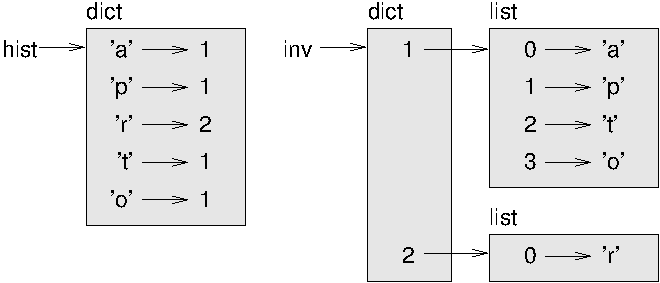
\includegraphics[scale=0.8]{figs/dict1.pdf}}
 \caption{Διάγραμμα κατάστασης.} 
\label{fig.dict1}
\end{figure}

 Η εικόνα ~\ref{fig.dict1}  είναι ένα διάγραμμα κατάστασης το οποίο δείχνει το  {\tt hist}  και το  {\tt inverse}.  Ένα λεξικό αναπαριστάται από ένα κουτί με τον τύπο  {\tt dict}  από πάνω του και τα ζευγάρια κλειδιού-τιμής μέσα του. Αν οι τιμές είναι ακέραιοι, δεκαδικοί ή συμβολοσειρές, τις σχεδιάζω συνήθως μέσα στο κουτί, αλλά αν είναι λίστες τότε απέξω, για να κρατάω το διάγραμμα απλό.
\index{state diagram}
\index{diagram!state}

Οι λίστες μπορεί να είναι τιμές σε ένα λεξικό, όπως είδαμε σε αυτό το παράδειγμα, αλλά δεν μπορεί να είναι κλειδιά. Να τι θα συμβεί αν δοκιμάσετε κάτι τέτοιο :
\index{TypeError}
\index{exception!TypeError}


\begin{verbatim}
>>> t = [1, 2, 3]
>>> d = dict()
>>> d[t] = 'oops'
Traceback (most recent call last):
  File "<stdin>", line 1, in ?
TypeError: list objects are unhashable
\end{verbatim}
%
 Όπως ανέφερα προηγουμένως, ένα λεξικό υλοποιείται χρησιμοποιώντας έναν πίνακα κατακερματισμού και αυτό σημαίνει ότι τα κλειδιά πρέπει να είναι  " κατακερματίσημα ".
\index{hash function}
\index{hashable}

 Συνάρτηση κατακερματισμού είναι μία συνάρτηση η οποία παίρνει μία τιμή (οποιουδήποτε τύπου) και επιστρέφει έναν ακέραιο αριθμό. Τα λεξικά χρησιμοποιούν αυτούς τους ακέραιους, οι οποίοι ονομάζονται τιμές κατακερματισμού ή αλλιώς τιμές κατατεμαχισμού, για να αποθηκεύουν και να αναζητούν ζευγάρια κλειδιού-τιμής.
\index{immutability}

Αυτό το σύστημα δουλεύει μια χαρά αν τα κλειδιά είναι αμετάβλητα. Αλλά αν τα κλειδιά είναι ευμετάβλητα, όπως είναι λίστες, τότε συμβαίνουν  " κακά πράγματα ".  Για παράδειγμα, όταν δημιουργείτε ένα ζευγάρι κλειδιού-τιμής, η  Python  κατακερματίζει το κλειδί και το αποθηκεύει στην αντίστοιχη θέση. Αν τροποποιήσετε το κλειδί και το επανακατακερματίσετε τότε θα πάει σε διαφορετική θέση. Σε αυτήν την περίπτωση ή θα έχετε δύο εγγραφές για το ίδιο κλειδί ή δεν θα μπορείτε να βρείτε κανένα κλειδί. Σε κάθε περίπτωση, το λεξικό δεν θα δουλεύει σωστά.

Γι' αυτόν το λόγο τα κλειδιά πρέπει να είναι κατακερματίσημα, και για αυτό οι ευμετάβλητοι τύποι όπως οι λίστες είναι ακατάλληλοι. Ο απλούστερος τρόπος για να ξεφύγουμε από αυτόν τον περιορισμό είναι να χρησιμοποιήσουμε πλειάδες, τις οποίες θα τις δούμε στο επόμενο κεφάλαιο.

Από τη στιγμή που τα λεξικά είναι ευμετάβλητα δεν μπορούν να χρησιμοποιηθούν σαν κλειδιά, αλλά μπορούν να χρησιμοποιηθούν σαν τιμές.

\begin{exercise}

Διαβάστε την τεκμηρίωση της μεθόδου των λεξικών  {\tt setdefault}  και χρησιμοποιήστε την για να γράψετε μία πιο λακωνική έκδοση της  \verb"invert_dict".  Λύση : \url{http://thinkpython.com/code/invert_dict.py}.
\end{exercise}
\index{setdefault method}
\index{method!setdefault}


 
\section{Σημείωμα}

Αν παίξατε με τη συνάρτηση  {\tt fibonacci}  της Ενότητας~ \ref{one.more.example},  θα παρατηρήσατε ίσως ότι όσο μεγαλύτερο όρισμα παρέχετε, τόσο περισσότερο χρόνο χρειάζεται η συνάρτηση για να τρέξει. Επιπροσθέτως, ο χρόνος εκτέλεσης αυξάνεται πολύ γρήγορα.
\index{fibonacci function}
\index{function!fibonacci}

Για να καταλάβετε το γιατί, μελετήστε την Εικόνα~ \ref{fig.fibonacci},  η οποία δείχνει το διάγραμμα κλήσεων για την  {\tt fibonacci}  με  {\tt n=4}:

\begin{figure}
\centerline
{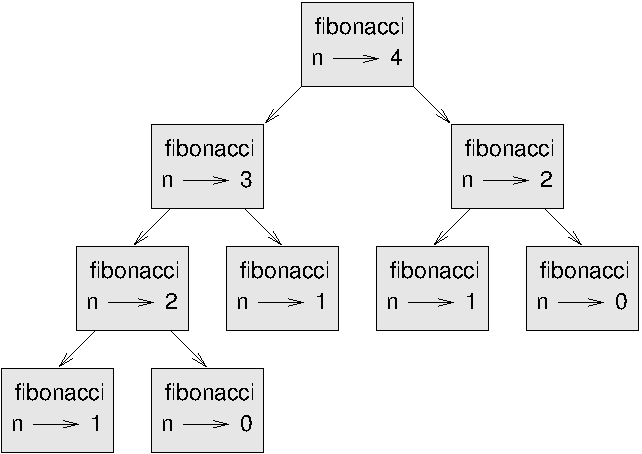
\includegraphics[scale=0.7]{figs/fibonacci.pdf}}
 \caption{Διάγραμμα κλήσεων.} 
\label{fig.fibonacci}
\end{figure}

 Ένα διάγραμμα κλήσεων δείχνει ένα σύνολο από πλαίσια συναρτήσεων με γραμμές οι οποίες συνδέουν κάθε πλαίσιο με τα πλαίσια των συναρτήσεων που αυτό καλεί. Στην κορυφή του διαγράμματος, η  {\tt fibonacci}  με  {\tt n=4}  καλεί την  {\tt fibonacci}  με  {\tt n=3}  και  {\tt n=2}.  Με τη σειρά της, η  {\tt fibonacci}  με  {\tt n=3}  καλεί τη  {\tt fibonacci}  με {\tt n=2}  και  {\tt n=1}  και ούτω καθεξής.
\index{function frame}
\index{frame}
\index{call graph}

 Μετρήστε πόσες φορές καλέστηκαν οι  {\tt fibonacci(0)}  και  {\tt fibonacci(1)}.  Αυτή η λύση είναι αναποδοτική και χειροτερεύει όσο μεγαλώνει το όρισμα.
\index{memo}

Μία άλλη λύση είναι να παρακολουθούμε τις τιμές οι οποίες έχουν ήδη υπολογιστεί αποθηκεύοντάς τες σε ένα λεξικό. Μία ήδη υπολογισμένη τιμή η οποία αποθηκεύτηκε για μεταγενέστερη χρήση ονομάζεται σημείωμα. Αυτή είναι μία υλοποίηση της  {\tt fibonacci}  χρησιμοποιώντας σημειώματα : 

\begin{verbatim}
known = {0:0, 1:1}

def fibonacci(n):
    if n in known:
        return known[n]

    res = fibonacci(n-1) + fibonacci(n-2)
    known[n] = res
    return res
\end{verbatim}
%
 Το  {\tt known}  είναι ένα λεξικό το οποίο κρατάει όλους τους αριθμούς  Fibonacci  που ήδη ξέρουμε. Ξεκινάει με δύο αντικείμενα :  το 0 αντιστοιχεί στο 0 και το 1 αντιστοιχεί στο 1.

Κάθε φορά που καλείται η  {\tt fibonacci}  ελέγχει το  {\tt known}.  Αν το αποτέλεσμα υπάρχει ήδη εκεί επιστρέφει αμέσως. Αλλιώς, πρέπει να υπολογίσει τη νέα τιμή, να την προσθέσει στο λεξικό και να την επιστρέψει.

\begin{exercise}

Τρέξτε αυτήν την έκδοση της  {\tt fibonacci}  και την αρχική με ένα εύρος παραμέτρων και συγκρίνετε τους χρόνους εκτέλεσης.

\end{exercise}

\begin{exercise}

Τροποποιήστε τη συνάρτηση του Άκερμαν της άσκησης~ \ref{ackermann}  χρησιμοποιώντας σημειώματα και δείτε αν είναι δυνατόν να υπολογίσετε τη συνάρτηση με μεγαλύτερα ορίσματα. Σημείωση :  όχι. Λύση : \url{http://thinkpython.com/code/ackermann_memo.py}.
\end{exercise}
\index{Ackermann function}
\index{function!ack}


 
\section{Καθολικές μεταβλητές}
\index{global variable}
\index{variable!global}

Στο προηγούμενο παράδειγμα, το  {\tt known}  δημιουργείται εκτός της συνάρτησης, άρα υπάγεται στο ειδικό πλαίσιο που ονομάζεται  \verb"__main__".  Συνήθως, οι μεταβλητές στη  \verb"__main__"  ονομάζονται καθολικές επειδή μπορούν να προσπελαστούν από οποιαδήποτε συνάρτηση. Αντιθέτως με τις τοπικές μεταβλητές, οι οποίες εξαφανίζονται όταν τελειώσει η συνάρτηση η οποία τις δημιούργησε, οι καθολικές μεταβλητές εξακολουθούν να υπάρχουν από τη μία κλήση συνάρτησης στην επόμενη.
\index{flag}

Οι καθολικές μεταβλητές χρησιμοποιούνται συχνά για  {\bf flags},  οι οποίες είναι μεταβλητές αληθείας που δείχνουν τη   " σημαία "  όταν μία συνθήκη είναι αληθής. Για παράδειγμα, μερικά προγράμματα χρησιμοποιούν μία σημαία με όνομα  {\tt verbose}  για  να ελέγχουν με ακρίβεια την έξοδο :

\begin{verbatim}
verbose = True

def example1():
    if verbose:
        print 'Running example1'
\end{verbatim}
%
 Αν προσπαθήσετε να αλλάξετε την τιμή μίας καθολικής μεταβλητής, μάλλον θα εκπλαγείτε. Το ακόλουθο παράδειγμα υποτίθεται ότι ελέγχει εάν έχει κληθεί η συνάρτηση :
\index{multiple assignment}
\index{assignment!multiple}

\begin{verbatim}
been_called = False

def example2():
    been_called = True         # WRONG
\end{verbatim}
%
 Αλλά αν το τρέξετε θα δείτε ότι η τιμή της  \verb"been_called"  δεν έχει αλλάξει. Το πρόβλημα είναι ότι η  {\tt example2}  δημιουργεί μία νέα τοπική μεταβλητή με όνομα  \verb"been_called"  η οποία χάνεται όταν τελειώσει η συνάρτηση χωρίς να επηρεάζει την καθολική μεταβλητή.
\index{global statement}
\index{statement!global}
\index{declaration}

Για να τροποποιήσετε μία καθολική μεταβλητή μέσα σε μία συνάρτηση πρέπει να δηλώσετε τη καθολική μεταβλητή πριν τη χρησιμοποιήσετε :

\begin{verbatim}
been_called = False

def example2():
    global been_called
    been_called = True
\end{verbatim}
%
 Η διασαφήνιση  {\tt global}  λέει στο διερμηνέα κάτι τέτοιο : " Σε αυτήν την συνάρτηση, όταν λέω  \verb"been_called",  εννοώ την καθολική μεταβλητή, μην δημιουργείς νέα τοπική ".
\index{update!global variable}
\index{global variable!update}

 Αυτό είναι ένα παράδειγμα το οποίο προσπαθεί να ενημερώσει μία καθολική μεταβλητή :

\begin{verbatim}
count = 0

def example3():
    count = count + 1          # WRONG
\end{verbatim}
%
 Αν το τρέξετε θα πάρετε :
\index{UnboundLocalError}
\index{exception!UnboundLocalError}

\begin{verbatim}
UnboundLocalError: local variable 'count' referenced before assignment
\end{verbatim}
%
 Η  Python  υποθέτει ότι η  {\tt count}  είναι τοπική, το οποίο σημαίνει ότι προσπαθείτε να την διαβάσετε προτού της εκχωρήσετε τιμή. Η λύση είναι πάλι να δηλώσετε την  {\tt count}  σαν καθολική :
\index{counter}

\begin{verbatim}
def example3():
    global count
    count += 1
\end{verbatim}
%
 Αν η καθολική μεταβλητή είναι ευμετάβλητη, μπορείτε να την τροποποιήσετε χωρίς να τη δηλώσετε :
\index{mutability}

\begin{verbatim}
known = {0:0, 1:1}

def example4():
    known[2] = 1
\end{verbatim}
%
 Επομένως, μπορείτε να προσθέσετε, να αφαιρέσετε και να αντικαταστήσετε τα στοιχεία μίας καθολικής λίστας ή ενός λεξικού, αλλά αν θέλετε να αλλάξετε την τιμή της μεταβλητής πρέπει να τη δηλώσετε :

\begin{verbatim}
def example5():
    global known
    known = dict()
\end{verbatim}
%

 
\section{Ακέραιοι μεγάλου μήκους}
\index{long integer}
\index{integer!long}
\index{type!long}

Αν υπολογίσετε την  {\tt fibonacci(50)}  θα πάρετε :

\begin{verbatim}
>>> fibonacci(50)
12586269025L
\end{verbatim}
%
 Το  {\tt L}  στο τέλος υποδεικνύει ότι το αποτέλεσμα είναι ένας ακέραιος αριθμός μεγάλου μήκους  {\tt long}.  Αυτός ο τύπος μεταβλητής δεν υπάρχει στην  Python 3,  όλοι οι ακέραιοι, ακόμα και οι πολύ μεγάλοι είναι τύπου  {\tt int}.
\index{Python 3}

 Οι τιμές με τύπο  {\tt int}  έχουν περιορισμένο εύρος. Οι ακέραιοι μεγάλου μήκους μπορεί ναι είναι αυθαίρετα μεγάλοι, αλλά όσο μεγαλώνουν καταναλώνουν περισσότερο χώρο και χρόνο.

Τόσο οι μαθηματικοί τελεστές όσο και οι συναρτήσεις της μονάδας λογισμικού  {\tt math}  δουλεύουν και στους ακέραιους μεγάλου μήκους. Επομένως, σε γενικές γραμμές, οποιοσδήποτε κώδικας δουλεύει με  {\tt int}  θα δουλεύει και με  
{\tt long}.

 Κάθε φορά που το αποτέλεσμα ενός υπολογισμού είναι πολύ μεγάλο για να αναπαρασταθεί από έναν ακέραιο, η  Python  μετατρέπει το αποτέλεσμα σε ένα ακέραιο μεγάλου μήκους :

\begin{verbatim}
>>> 1000 * 1000
1000000
>>> 100000 * 100000
10000000000L
\end{verbatim}
%
 Στην πρώτη περίπτωση, το αποτέλεσμα έχει τύπο  {\tt int},  ενώ στη δεύτερη είναι  {\tt long}.

\begin{exercise}
\index{encryption}
\index{RSA algorithm}
\index{algorithm!RSA}

Η ύψωση σε δύναμη μεγάλων ακεραίων είναι η βάση των πιο συνηθισμένων αλγορίθμων κρυπτογράφησης δημόσιου κλειδιού. Διαβάστε τη σελίδα της  Wikipedia  για τον αλγόριθμο  RSA (\url{http://en.wikipedia.org/wiki/RSA})  και γράψτε συναρτήσεις οι οποίες θα κωδικοποιούν και θα αποκωδικοποιούν μηνύματα.
\end{exercise}
% TODO: solution for this one!



\section{Αποσφαλμάτωση}
\index{debugging}

Καθώς θα εργάζεστε με όλο και μεγαλύτερα σύνολα δεδομένων, η χειροκίνητη αποσφαλμάτωση με εμφάνιση και έλεγχο δεδομένων μπορεί να γίνει ιδιαίτερα δύσχρηστη. Αυτές είναι μερικές υποδείξεις για την αποσφαλμάτωση μεγάλων όγκων δεδομένων :

\begin{description}

\item [ Περιορίστε την είσοδο :]   Μειώστε το μέγεθος του συνόλου δεδομένων αν είναι δυνατό. Για παράδειγμα, αν το πρόγραμμα διαβάζει ένα αρχείο κειμένου, ξεκινήστε μόνο με τις πρώτες 10 γραμμές ή με το μικρότερο παράδειγμα που μπορείτε να βρείτε. Μπορείτε είτε να επεξεργαστείτε τα ίδια τα αρχεία, είτε (καλύτερα) να τροποποιήσετε το πρόγραμμα ούτως ώστε να διαβάζει μόνο τις πρώτες  {\tt n}  γραμμές.

Αν προκύψει κάποιο σφάλμα, μπορείτε να μειώσετε το  {\tt n}  στη μικρότερη τιμή που εμφανίζεται το σφάλμα και στη συνέχεια να την αυξάνετε σταδιακά όσο εντοπίζετε και διορθώνετε λάθη.

 \item[  Ελέγξτε συνόψεις και τύπους:]   Αντί να εμφανίζετε και να ελέγχετε ολόκληρο το σύνολο δεδομένων, δοκιμάστε να εμφανίσετε συνόψεις των δεδομένων. Για  παράδειγμα, μια σύνοψη μπορεί να είναι ο πλήθος των αντικειμένων ενός λεξικού ή το σύνολο 
των αριθμών μίας λίστας.

Μία συχνή αιτία για τα σφάλματα χρόνου εκτέλεσης είναι μία τιμή με λάθος τύπο δεδομένων. Για την αποσφαλμάτωση αυτού του τύπου σφάλματος, τις περισσότερες φορές αρκεί να εμφανίσουμε τον τύπο μίας μεταβλητής.

 \item[ Γράψτε αυτοελέγχους:]   Μερικές φορές μπορείτε να γράψετε κώδικα ο οποίος θα ελέγχει για σφάλματα αυτόματα. Για παράδειγμα, αν υπολογίζατε το μέσο όρο μίας λίστας αριθμών, θα μπορούσατε να ελέγξετε ότι το αποτέλεσμα δεν είναι μεγαλύτερο από το μεγαλύτερο στοιχείο της λίστας ή μικρότερο από το μικρότερο στοιχείο. Αυτός ονομάζεται  " λογικός έλεγχος "  γιατί ανιχνεύει αποτελέσματα τα οποία είναι  " παράλογα ".
\index{sanity check}
\index{consistency check}

 Ένα άλλο είδος ελέγχου συγκρίνει τα αποτελέσματα από δύο διαφορετικούς υπολογισμούς για να δει αν συνάδουν. Αυτός ονομάζεται  " έλεγχος συνέπειας ".

\item[ Ομορφύνετε την έξοδο :]  Η μορφοποίηση της εξόδου αποσφαλμάτωσης μπορεί  να κάνει ευκολότερο τον εντοπισμό ενός λάθους. Είδαμε ένα τέτοιο παράδειγμα στην Ενότητα~ \ref{factdebug}.  Η μονάδα λογισμικού  {\tt pprint}  παρέχει μία συνάρτηση  {\tt pprint}  η οποία εμφανίζει τους ενσωματωμένους τύπους σε μία πιο ευανάγνωστη μορφή. 
\index{pretty print}
\index{pprint module}
\index{module!pprint}

\end{description}

 Και πάλι, ο χρόνος που ξοδεύετε για να φτιάξετε μία σκαλωσιά μπορεί να μειώσει το χρόνο που θα ξοδεύατε για αποσφαλμάτωση.
\index{scaffolding}

`\section{Ορολογία}
 
\begin{description}

\item[ λεξικό :]  Μία αντιστοίχιση ενός συνόλου κλειδιών με τις αντίστοιχες τιμές τους.
\index{dictionary}

 \item[ ζευγάρι κλειδιού-τιμής :]  Η αναπαράσταση μίας αντιστοίχισης ενός κλειδιού με μία τιμή.
\index{key-value pair}

 \item[ αντικείμενο:]  Μία άλλη ονομασία για ένα ζευγάρι κλειδιού-τιμής.
\index{item!dictionary}

 \item[ κλειδί :]  Ένα αντικείμενο το οποίο εμφανίζεται μέσα σε ένα λεξικό σαν το πρώτο μέρος ενός ζευγαριού κλειδιού-τιμής.
\index{key}

 \item[ τιμή :]  Ένα αντικείμενο το οποίο εμφανίζεται μέσα σε ένα λεξικό σαν το δεύτερο μέρος ενός ζευγαριού κλειδιού-τιμής. Αυτή είναι πιο συγκεκριμένη χρήση της λέξης  " τιμή "  σε σχέση με την προηγούμενη.
\index{value}

 \item[ υλοποίηση :]  Ένας τρόπος εκτέλεσης ενός υπολογισμού.
\index{implementation}

 \item[ πίνακας κατακερματισμού :]  Ο αλγόριθμος που χρησιμοποιείται για να υλοποιήσει λεξικά στην  Python.
\index{hashtable}

\item[ συνάρτηση κατακερματισμού :]  Μία συνάρτηση που χρησιμοποιείται από ένα πίνακα κατακερματισμού για να υπολογίσει την θέση ενός κλειδιού.
\index{hash function}

 \item[ κατακερματίσημος :]  Ένας τύπος ο οποίος έχει μία συνάρτηση κατακερματισμού. Οι αμετάβλητοι τύποι όπως οι ακέραιοι, οι δεκαδικοί και οι συμβολοσειρές είναι κατακερματίσημοι, ενώ οι ευμετάβλητοι τύποι όπως είναι οι λίστες και τα λεξικά δεν είναι.
\index{hashable}

 \item[ αναζήτηση :]  Μία διαδικασία η οποία παίρνει ένα κλειδί και βρίσκει την αντίστοιχη τιμή.
\index{lookup}

 \item[ αντίστροφη αναζήτηση :]  Μία διαδικασία η οποία  παίρνει μία τιμή και βρίσκει ένα ή περισσότερα κλειδιά τα οποία της αντιστοιχούν.
\index{reverse lookup, dictionary}

 \item[ μονήρης :]  Μία λίστα (ή κάποια άλλη ακολουθία) με μόνο ένα στοιχείο.
\index{singleton}

 \item[ διάγραμμα κλήσεων :]  Ένα διάγραμμα το οποίο δείχνει κάθε πλαίσιο το οποίο δημιουργείται κατά την εκτέλεση ενός προγράμματος, με ένα βέλος από τον κάθε καλούντα στον κάθε καλούμενο.
\index{call graph}
\index{diagram!call graph}

 \item[ ιστόγραμμα :]  Ένα σύνολο από μετρητές.
\index{histogram}

 \item[ σημείωμα :]  Μία ήδη υπολογισμένη τιμή η οποία αποθηκεύεται για την αποφυγή περιττού υπολογισμού στο μέλλον.
\index{memo}

 \item[ καθολική μεταβλητή :]   Μία μεταβλητή η οποία ορίζεται έξω από μία συνάρτηση. Οι καθολικές μεταβλητές μπορούν να προσπελαστούν από οποιαδήποτε συνάρτηση.
\index{global variable}

 \item[ σημαία :]  Μία μεταβλητή αληθείας η οποία χρησιμοποιείται για να υποδείξει αν μία συνθήκη είναι αληθής ή όχι.
\index{flag}

 \item[ διασαφήνιση :]  Μία δήλωση όπως η  {\tt global}  η οποία λέει στο διερμηνέα κάτι σχετικά με μία μεταβλητή.
\index{declaration}

\end{description}

 
\section{Ασκήσεις}

\begin{exercise}
\index{duplicate}

Αν κάνατε την Άσκηση~ \ref{duplicate},  έχετε ήδη μία συνάρτηση με όνομα  \verb"has_duplicates"  η οποία παίρνει μία λίστα σαν παράμετρο και επιστρέφει  {\tt True}  αν υπάρχει τουλάχιστον ένα αντικείμενο το οποίο εμφανίζεται περισσότερες από μία φορά μέσα στη λίστα.

Χρησιμοποιήστε ένα λεξικό για να γράψετε μία πιο γρήγορη και απλούστερη έκδοση της  \verb"has_duplicates".  Λύση : \url{http://thinkpython.com/code/has_duplicates.py}.

\end{exercise}


\begin{exercise}
\label{exrotatepairs}
\index{letter rotation}
\index{rotation!letters}

Δύο λέξεις είναι  " αντεστραμμένο ζεύγος "  αν περιστρέφοντας τη μία από αυτές παίρνετε την άλλη  ( δείτε την  \verb"rotate_word"  στην Άσκηση~ \ref{exrotate}).

 Γράψτε ένα πρόγραμμα το οποίο θα διαβάζει μία λίστα λέξεων και θα βρίσκει όλα τα αντεστραμμένα ζεύγη. Λύση : \url{http://thinkpython.com/code/rotate_pairs.py}.

\end{exercise}


\begin{exercise}
\index{Car Talk}
\index{Puzzler}

Αυτός είναι ένας ακόμα γρίφος από την   {\em Car
Talk} (\url{http://www.cartalk.com/content/puzzlers}):

\begin{quote}
 Αυτό το έστειλε ένας συνάδελφος, ο  Dan O'Leary,  ο οποίος πρόσφατα, έπεσε τυχαία πάνω σε μία συνηθισμένη μονοσύλλαβη λέξη πέντε γραμμάτων η οποία έχει την εξής μοναδική ιδιότητα. Όταν αφαιρέσετε το πρώτο γράμμα, τα υπόλοιπα σχηματίζουν ένα ομόφωνο της αρχικής λέξης, το οποίο είναι μία λέξη η οποία ακούγεται ακριβώς το ίδιο. Αντικαταστήστε το πρώτο γράμμα, ήτοι, βάλτε το πάλι πίσω και αφαιρέστε το δεύτερο γράμμα και το αποτέλεσμα είναι πάλι ένα ομόφωνο της αρχικής λέξης. Και η ερώτηση είναι, ποια είναι η λέξη ; 

 Τώρα θα σας δώσω ένα παράδειγμα το οποίο όμως δεν δουλεύει. Ας δούμε την πέντε γραμμάτων λέξη  "wrack". W-R-A-C-K,  όπως λέμε  "wrack with pain"  (ταλαιπωρήστε από τον πόνο). Αν αφαιρέσω το πρώτο γράμμα, μου μένει μία λέξη με τέσσερα γράμματα, η  "R-A-C-K".  Όπως λέμε : `Holy cow, did you see the rack on that buck! It must have been a nine-pointer!'  Είναι ένα τέλειο ομόφωνο. Αντ' αυτού, αν ξαναβάλετε πίσω το γράμμα  'w'  και αφαιρέσετε το  'r'  θα προκύψει η λέξη  "wack",  η οποία είναι μία πραγματική λέξη, δεν είναι ομόφωνο από τις άλλες δύο λέξεις. 

Αλλά υπάρχει, ωστόσο, τουλάχιστον μία λέξη την οποία γνωρίζουμε και η οποία αποδίδει δύο ομόφωνα αν αφαιρέσετε ένα από τα δύο πρώτα γράμματα φτιάχνοντας δύο νέες λέξεις τεσσάρων γραμμάτων. Η ερώτηση είναι , ποια είναι η λέξη ;
\end{quote}
\index{homophone}
\index{reducible word}
\index{word, reducible}

 Μπορείτε να χρησιμοποιήσετε το λεξικό της Άσκησης~ \ref{wordlist2}  για να ελέγξετε αν μία συμβολοσειρά υπάρχει μέσα στη λίστα λέξεων.

Για να ελέγξετε αν δύο λέξεις είναι ομόφωνα, μπορείτε να χρησιμοποιήσετε το λεξικό προφοράς  CMU.  Μπορείτε να το κατεβάσετε από το σύνδεσμο  \url{http://www.speech.cs.cmu.edu/cgi-bin/cmudict}  ή από τον σύνδεσμο  \url{http://thinkpython.com/code/c06d}  και επίσης μπορείτε να κατεβάσετε και το  \url{http://thinkpython.com/code/pronounce.py},  το οποίο παρέχει μία συνάρτηση με όνομα  \verb"read_dictionary"  η οποία  διαβάζει το λεξικό προφοράς και επιστρέφει ένα λεξικό σε  Python  το οποίο αντιστοιχεί κάθε λέξη σε μία συμβολοσειρά η οποία περιγράφει την βασική προφορά της.

Γράψτε ένα πρόγραμμα το οποίο θα εμφανίζει όλες τις λέξεις η οποίες επιλύουν το γρίφο. 
Λύση : \url{http://thinkpython.com/code/homophone.py}.

\end{exercise}

 
 
\chapter{Πλειάδες}
\label{tuplechap}

\section{Οι πλειάδες είναι αμετάβλητες}
\index{tuple}
\index{type!tuple}
\index{sequence}

Μία πλειάδα είναι μία ακολουθία τιμών οποιουδήποτε τύπου οι οποίες ευρετηριάζονται με  ακεραίους αριθμούς. Από αυτήν την άποψη οι πλειάδες μοιάζουν πολύ με τις λίστες. Η σημαντική διαφορά είναι ότι οι λίστες είναι αμετάβλητες. 
\index{mutability}
\index{immutability}

Συντακτικά, μία πλειάδα είναι μία λίστα τιμών χωρισμένες με κόμματα :

\begin{verbatim}
>>> t = 'a', 'b', 'c', 'd', 'e'
\end{verbatim}
%
 Παρόλο που δεν είναι απαραίτητο, συνηθίζεται να εμπερικλείουμε τις πλειάδες μέσα σε παρενθέσεις :
\index{parentheses!tuples in}

\begin{verbatim}
>>> t = ('a', 'b', 'c', 'd', 'e')
\end{verbatim}
%
 Για να δημιουργήσετε μία πλειάδα με μόνο ένα στοιχείο, θα πρέπει να συμπεριλάβετε ένα κόμμα στο τέλος :
\index{singleton}
\index{tuple!singleton}

\begin{verbatim}
>>> t1 = 'a',
>>> type(t1)
<type 'tuple'>
\end{verbatim}
%
 Μία τιμή μέσα σε παρενθέσεις δεν είναι πλειάδα :

\begin{verbatim}
>>> t2 = ('a')
>>> type(t2)
<type 'str'>
\end{verbatim}
%
 Ένας άλλος τρόπος για να δημιουργήσετε μία πλειάδα είναι ενσωματωμένη συνάρτηση  {\tt tuple}.  Χωρίς ορίσματα δημιουργεί μία κενή πλειάδα :
\index{tuple function}
\index{function!tuple}

\begin{verbatim}
>>> t = tuple()
>>> print t
()
\end{verbatim}
%
 Αν το όρισμα είναι μία ακολουθία (συμβολοσειρά, λίστα ή πλειάδα), το αποτέλεσμα είναι μία πλειάδα με τα στοιχεία της ακολουθίας :

\begin{verbatim}
>>> t = tuple('lupins')
>>> print t
('l', 'u', 'p', 'i', 'n', 's')
\end{verbatim}
%
 Επειδή το  {\tt tuple}  είναι το όνομα μίας ενσωματωμένης συνάρτησης θα πρέπει να αποφεύγετε να το χρησιμοποιείτε σαν όνομα μεταβλητής.

Οι περισσότεροι τελεστές που χρησιμοποιούνται στις λίστες δουλεύουν και με τις πλειάδες. Για παράδειγμα, ο τελεστής αγκύλης δείχνει ένα στοιχείο :
\index{bracket operator}
\index{operator!bracket}

\begin{verbatim}
>>> t = ('a', 'b', 'c', 'd', 'e')
>>> print t[0]
'a'
\end{verbatim}
%
 Και ο τελεστής τεμαχίου επιλέγει ένα εύρος στοιχείων :
\index{slice operator}
\index{operator!slice}
\index{tuple!slice}
\index{slice!tuple}

\begin{verbatim}
>>> print t[1:3]
('b', 'c')
\end{verbatim}
%
 Αλλά αν προσπαθήσετε να τροποποιήσετε ένα από τα στοιχεία της πλειάδας, θα πάρετε ένα λάθος :
\index{exception!TypeError}
\index{TypeError}
\index{item assignment}
\index{assignment!item}

\begin{verbatim}
>>> t[0] = 'A'
TypeError: object doesn't support item assignment
\end{verbatim}
%
 Δεν μπορείτε να τροποποιήσετε τα στοιχεία μίας πλειάδας, αλλά μπορείτε να αντικαταστήσετε μία πλειάδα με μία άλλη :

\begin{verbatim}
>>> t = ('A',) + t[1:]
>>> print t
('A', 'b', 'c', 'd', 'e')
\end{verbatim}
%

 
\section{Εκχώρηση πλειάδων}
\label{tuple.assignment}
\index{tuple!assignment}
\index{assignment!tuple}
\index{swap pattern}
\index{pattern!swap}

Είναι συχνά χρήσιμο να αντιμεταθέτουμε τις τιμές δύο μεταβλητών. Με τις συμβατικές εκχωρήσεις είναι απαραίτητο να χρησιμοποιήσετε μία προσωρινή μεταβλητή. Για παράδειγμα, για να αντιμεταθέσετε την  {\tt a}  και την  {\tt b}:

\begin{verbatim}
>>> temp = a
>>> a = b
>>> b = temp
\end{verbatim}
%
 Αυτή η λύση είναι κάπως επαχθής σε σχέση με την εκχώρηση πλειάδων, η οποία είναι πιο κομψή :

\begin{verbatim}
>>> a, b = b, a
\end{verbatim}
%
 Στην αριστερή πλευρά είναι μία πλειάδα μεταβλητών και στη δεξιά πλευρά είναι μία πλειάδα εκφράσεων. Κάθε τιμή εκχωρείται στην αντίστοιχη μεταβλητή. Όλες οι εκφράσεις στην δεξιά πλευρά υπολογίζονται πριν από οποιαδήποτε εκχώρηση.

Το πλήθος των μεταβλητών στα αριστερά και το πλήθος των τιμών στα δεξιά πρέπει να είναι τα ίδια :
\index{exception!ValueError}
\index{ValueError}

\begin{verbatim}
>>> a, b = 1, 2, 3
ValueError: too many values to unpack
\end{verbatim}
%
 Γενικότερα, η δεξιά πλευρά μπορεί να είναι οποιοδήποτε είδος ακολουθίας (συμβολοσειρά, λίστα ή πλειάδα). Για παράδειγμα, για να χωρίσετε μία διεύθυνση ηλεκτρονικού ταχυδρομείου στο όνομα χρήστη και στον τομέα, θα μπορούσατε να γράψετε : 
\index{split method}
\index{method!split}
\index{email address}

\begin{verbatim}
>>> addr = 'monty@python.org'
>>> uname, domain = addr.split('@')
\end{verbatim}
%
 Η επιστρεφόμενη τιμή από την  {\tt split}  είναι μία λίστα με δύο στοιχεία. Το πρώτο στοιχείο εκχωρείται στην  {\tt uname}  και το δεύτερο στην  {\tt domain}.

\begin{verbatim}
>>> print uname
monty
>>> print domain
python.org
\end{verbatim}
%

 
\section{Οι πλειάδες σαν επιστρεφόμενες τιμές}
\index{tuple}
\index{value!tuple}
\index{return value!tuple}
\index{function, tuple as return value}

Στην πραγματικότητα, μία συνάρτηση μπορεί να επιστρέψει μόνο μία τιμή, αλλά αν η τιμή είναι μία πλειάδα τότε είναι σαν να επιστρέφει πολλές τιμές. Για παράδειγμα, αν θέλατε να διαιρέσετε δύο ακέραιους και να υπολογίσετε το πηλίκο και το υπόλοιπο είναι προτιμότερο να τα υπολογίσετε ταυτόχρονα παρά να υπολογίσετε πρώτα το  {\tt x/y}  και μετά το  {\tt x\%y}.
\index{divmod}

 Η ενσωματωμένη συνάρτηση  {\tt divmod}  παίρνει δύο ορίσματα και επιστρέφει μία πλειάδα δύο τιμών, το πηλίκο και το υπόλοιπο. Μπορείτε να αποθηκεύσετε το αποτέλεσμα σαν μία πλειάδα :

\begin{verbatim}
>>> t = divmod(7, 3)
>>> print t
(2, 1)
\end{verbatim}
%
 Ή να αποθηκεύσετε τα στοιχεία χωριστά χρησιμοποιώντας εκχώρηση πλειάδας :
\index{tuple assignment}
\index{assignment!tuple}

\begin{verbatim}
>>> quot, rem = divmod(7, 3)
>>> print quot
2
>>> print rem
1
\end{verbatim}
%
 Αυτό είναι ένα παράδειγμα μιας συνάρτησης η οποία επιστρέφει μία πλειάδα :

\begin{verbatim}
def min_max(t):
    return min(t), max(t)
\end{verbatim}
%
 Η  {\tt max}  και η  {\tt min}  είναι ενσωματωμένες συναρτήσεις η οποίες βρίσκουν το μεγαλύτερο και το μικρότερο στοιχείο μίας ακολουθίας. Η  \verb"min_max"  υπολογίζει και τα δύο και επιστρέφει μία πλειάδα δύο τιμών.
\index{max function}
\index{function!max}
\index{min function}
\index{function!min}


 
\section{Οι πλειάδες σαν ορίσματα μεταβλητού μήκους}
\index{variable-length argument tuple}
\index{argument!variable-length tuple}
\index{gather}
\index{parameter!gather}
\index{argument!gather}

Οι συναρτήσεις μπορούν να πάρουν ένα μεταβλητό πλήθος από ορίσματα. Μία παράμετρος το όνομα της οποίας ξεκινάει με  {\tt *}  συσσωρεύει ορίσματα σε μία πλειάδα. Για παράδειγμα, η  {\tt printall}  παίρνει οποιοδήποτε πλήθος ορισμάτων και τα εμφανίζει  :

\begin{verbatim}
def printall(*args):
    print args
\end{verbatim}
%
 Η παράμετρος συσσώρευσης μπορεί να έχει οποιοδήποτε όνομα θέλετε, αλλά το πιο συνηθισμένο είναι το  {\tt args}.  Εδώ φαίνεται πως δουλεύει η συνάρτηση :

\begin{verbatim}
>>> printall(1, 2.0, '3')
(1, 2.0, '3')
\end{verbatim}
%
 Το σύνολο της συσσώρευσης είναι σκεδάσιμο, μπορεί δηλαδή να σπάσει στα επιμέρους στοιχεία. Αν έχετε μία ακολουθία από τιμές και θέλετε να την περάσετε σε μία συνάρτηση σαν πολλαπλά ορίσματα, μπορείτε να χρησιμοποιήσετε τον τελεστή  {\tt *}.  Για παράδειγμα, η  {\tt divmod}  παίρνει ακριβώς δύο ορίσματα, δεν δουλεύει με μία πλειάδα :

% removing this because we haven't seen optional parameters yet
%You can combine the gather operator with required and positional
%arguments:

%%\begin{verbatim}
%def pointless(required, optional=0, *args):
%    print required, optional, args
%\end{verbatim}
%\afterverb
%
%Run this function with 1, 2, 3 and 4 or more arguments and
%make sure you understand what it does.
\index{scatter}
\index{argument scatter}
\index{TypeError}
\index{exception!TypeError}

\begin{verbatim}
>>> t = (7, 3)
>>> divmod(t)
TypeError: divmod expected 2 arguments, got 1
\end{verbatim}
%
 Αλλά αν διαμερίσετε την πλειάδα, δουλεύει :

\begin{verbatim}
>>> divmod(*t)
(2, 1)
\end{verbatim}
%
\begin{exercise}

Πολλές από τις ενσωματωμένες συναρτήσεις χρησιμοποιούν μεταβλητού μήκους όρισμα πλειάδας. Για παράδειγμα, η  {\tt max}  και η  {\tt min}  μπορούν να πάρουν οποιοδήποτε αριθμό ορισμάτων :
\index{max function}
\index{function!max}
\index{min function}
\index{function!min}

\begin{verbatim}
>>> max(1,2,3)
3
\end{verbatim}
%
Η  {\tt sum}  όμως όχι :
\index{sum function}
\index{function!sum}

\begin{verbatim}
>>> sum(1,2,3)
TypeError: sum expected at most 2 arguments, got 3
\end{verbatim}
%
Γράψτε μία συνάρτηση με όνομα  {\tt sumall}  η οποία θα παίρνει οποιοδήποτε πλήθος ορισμάτων και θα επιστρέφει το άθροισμά τους.
\end{exercise}


\section{Λίστες και πλειάδες}
\index{zip function}
\index{function!zip}

Η  {\tt zip}  είναι μία ενσωματωμένη συνάρτηση η οποία παίρνει δύο ή περισσότερες ακολουθίες και τις  " ζιπάρει "  σε μία λίστα πλειάδων όπου η κάθε μία πλειάδα περιέχει ένα στοιχείο από κάθε ακολουθία. Στην  Python 3,  η  {\tt zip}  επιστρέφει ένα επαναλήπτη πλειάδων, αλλά τις περισσότερες φορές συμπεριφέρεται σαν μία λίστα.

Αυτό το παράδειγμα ζιπάρει μία συμβολοσειρά και μία λίστα :

\begin{verbatim}
>>> s = 'abc'
>>> t = [0, 1, 2]
>>> zip(s, t)
[('a', 0), ('b', 1), ('c', 2)]
\end{verbatim}
%
 Το αποτέλεσμα είναι μία λίστα από πλειάδες όπου κάθε πλειάδα περιέχει ένα χαρακτήρα από τη συμβολοσειρά και το αντίστοιχο στοιχείο από τη λίστα.
\index{list!of tuples}

Αν οι ακολουθίες δεν έχουν το ίδιο μήκος, το αποτέλεσμα έχει το μήκος της μικρότερης.

\begin{verbatim}
>>> zip('Anne', 'Elk')
[('A', 'E'), ('n', 'l'), ('n', 'k')]
\end{verbatim}
%
 Μπορείτε να χρησιμοποιήσετε εκχώρηση πλειάδας σε ένα βρόγχο  {\tt for}  για να διασχίσετε μία λίστα πλειάδων :
\index{traversal}
\index{tuple assignment}
\index{assignment!tuple}

\begin{verbatim}
t = [('a', 0), ('b', 1), ('c', 2)]
for letter, number in t:
    print number, letter
\end{verbatim}
%
 Σε κάθε επανάληψη, η  Python  επιλέγει την επόμενη πλειάδα μέσα στη λίστα και εκχωρεί τα στοιχεία στη  {\tt letter}  και στη  {\tt number}.  Η έξοδος αυτού του βρόγχου είναι :
\index{loop}

\begin{verbatim}
0 a
1 b
2 c
\end{verbatim}
%
 Αν συνδυάσετε την  {\tt zip},  την  {\tt for}  και την εκχώρηση πλειάδας, τότε προκύπτει ένα χρήσιμο ιδίωμα  για διάσχιση δύο (ή περισσότερων) ακολουθιών ταυτόχρονα. Για παράδειγμα, η  \verb"has_match"  παίρνει δύο ακολουθίες, την  {\tt t1}  και την  {\tt t2},  και επιστρέφει  {\tt True}  αν υπάρχει δείκτης τέτοιος ώστε  {\tt t1[i] == t2[i]}:
\index{for loop}

\begin{verbatim}
def has_match(t1, t2):
    for x, y in zip(t1, t2):
        if x == y:
            return True
    return False
\end{verbatim}
%
 Αν θέλετε να διασχίσετε τα στοιχεία μίας ακολουθίας μαζί με τους δείκτες τους, μπορείτε να χρησιμοποιήσετε την ενσωματωμένη συνάρτηση  {\tt enumerate}:
\index{traversal}
\index{enumerate function}
\index{function!enumerate}

\begin{verbatim}
for index, element in enumerate('abc'):
    print index, element
\end{verbatim}
%
 Η έξοδος αυτού του βρόγχου είναι :

\begin{verbatim}
0 a
1 b
2 c
\end{verbatim}
%
 Ξανά.


\section{Λεξικά και πλειάδες}
\label{dictuple}
\index{dictionary}
\index{items method}
\index{method!items}
\index{key-value pair}

Τα λεξικά έχουν μία μέθοδο με όνομα  {\tt items}  η οποία επιστρέφει μία λίστα από πλειάδες, όπου η κάθε πλειάδα είναι ένα ζευγάρι κλειδιού-τιμής.


\begin{verbatim}
>>> d = {'a':0, 'b':1, 'c':2}
>>> t = d.items()
>>> print t
[('a', 0), ('c', 2), ('b', 1)]
\end{verbatim}
%
 Όπως θα περιμένατε από ένα λεξικό, τα αντικείμενα δεν είναι ταξινομημένα. Στην  Python 3  η  {\tt items}  επιστρέφει  έναν επαναλήπτη, αλλά συνήθως, οι επαναλήπτες συμπεριφέρονται όπως οι λίστες.

Πηγαίνοντας αντίστροφα, μπορείτε να χρησιμοποιήσετε μία λίστα πλειάδων για να αρχικοποιήσετε ένα νέο λεξικό :
\index{dictionary!initialize}

\begin{verbatim}
>>> t = [('a', 0), ('c', 2), ('b', 1)]
>>> d = dict(t)
>>> print d
{'a': 0, 'c': 2, 'b': 1}
\end{verbatim}

 Συνδυάζοντας την  {\tt dict}  με την  {\tt zip}  προκύπτει ένας συνοπτικός τρόπος για τη δημιουργία ενός λεξικού :
\index{zip function!use with dict}

\begin{verbatim}
>>> d = dict(zip('abc', range(3)))
>>> print d
{'a': 0, 'c': 2, 'b': 1}
\end{verbatim}
%
 Η μέθοδος  {\tt update}  των λεξικών μπορεί επίσης να πάρει μία λίστα από πλειάδες και να τις προσθέσει, σαν ζευγάρια κλειδιού-τιμής, σε ένα υπάρχον λεξικό.
\index{update method}
\index{method!update}
\index{traverse!dictionary}
\index{dictionary!traversal}

Συνδυάζοντας την  {\tt items},  την εκχώρηση πλειάδων την  {\tt for},  προκύπτει το ιδίωμα για διάσχιση τόσο των κλειδιών όσο και των τιμών ενός λεξικού :

\begin{verbatim}
for key, val in d.items():
    print val, key
\end{verbatim}
%
 Η έξοδος αυτού του βρόγχου είναι :

\begin{verbatim}
0 a
2 c
1 b
\end{verbatim}
%
 Πάλι.

Είναι συνηθισμένο να χρησιμοποιούνται πλειάδες σαν κλειδιά μέσα σε ένα λεξικό, πρωτίστως γιατί δεν μπορούμε να χρησιμοποιήσουμε λίστες. Για παράδειγμα, ένας τηλεφωνικός κατάλογος μπορεί να αντιστοιχεί ζευγάρια επωνύμου, ονόματος σε τηλεφωνικούς αριθμούς. Θεωρώντας ότι έχουμε ορίσει την  {\tt last},  την  {\tt first}  και την  {\tt number},  θα μπορούσαμε να γράψουμε :
\index{tuple!as key in dictionary}
\index{hashable}

\begin{verbatim}
directory[last,first] = number
\end{verbatim}
%
 Η έκφραση μέσα στις αγκύλες είναι μία πλειάδα. Θα μπορούσαμε να χρησιμοποιήσουμε την εκχώρηση πλειάδων για να διασχίσουμε αυτό το λεξικό.
\index{tuple!in brackets}

 
\begin{verbatim}
for last, first in directory:
    print first, last, directory[last,first]
\end{verbatim}
%
 Αυτός ο βρόχος διασχίζει τα κλειδιά μέσα στο  {\tt directory},  τα οποία είναι πλειάδες. Εκχωρεί τα στοιχεία της κάθε πλειάδας στην  {\tt last}  και στην  {\tt first},  και μετά εμφανίζει το ονοματεπώνυμο με τον αντίστοιχο τηλεφωνικό αριθμό.

Υπάρχουν δύο τρόποι να αναπαραστήσουμε πλειάδες σε ένα διάγραμμα κατάστασης. Η πιο λεπτομερής εκδοχή δείχνει τους δείκτες και τα στοιχεία ακριβώς όπως εμφανίζονται μέσα σε μία λίστα. Για παράδειγμα, η πλειάδα  \verb"('Cleese', 'John')"  θα φαίνεται όπως στην Εικόνα ~\ref{fig.tuple1}.
\index{state diagram}
\index{diagram!state}

\begin{figure}
\centerline
{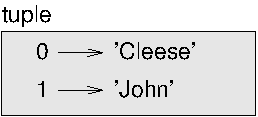
\includegraphics[scale=0.8]{figs/tuple1.pdf}}
 \caption{Διάγραμμα κατάστασης.} 
\label{fig.tuple1}
\end{figure}

 Αλλά σε ένα μεγαλύτερο διάγραμμα μπορεί να θέλετε να παραλήψετε τις λεπτομέρειες. Για παράδειγμα, ένα διάγραμμα του τηλεφωνικού καταλόγου θα μπορούσε να είναι όπως αυτό στην Εικόνα ~\ref{fig.dict2}.

\begin{figure}
\centerline
{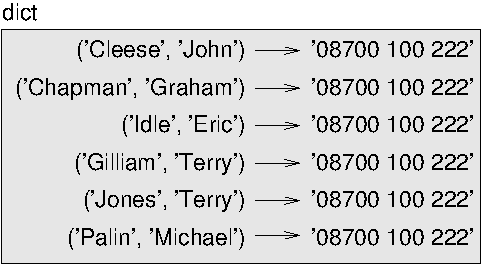
\includegraphics[scale=0.8]{figs/dict2.pdf}}
 \caption{Διάγραμμα κατάστασης}
\label{fig.dict2}
\end{figure}

 Εδώ οι πλειάδες εμφανίζονται χρησιμοποιώντας το συντακτικό της  Python  σαν μία γραφική στενογραφία.

Ο τηλεφωνικός αριθμός μέσα στο διάγραμμα είναι η γραμμή παραπόνων για το  BBC,  οπότε παρακαλώ μην τον καλέσετε.


\section{Συγκρίνοντας πλειάδες}
\index{comparison!tuple}
\index{tuple!comparison}
\index{sort method}
\index{method!sort}

Οι σχεσιακοί τελεστές δουλεύουν με τις πλειάδες και άλλες ακολουθίες. Η  Python  ξεκινάει συγκρίνοντας τα πρώτα στοιχεία  κάθε ακολουθίας. Αν είναι ίσα, πηγαίνει στα επόμενα, και ούτω καθεξής, μέχρι να βρει στοιχεία τα οποία είναι διαφορετικά. Τα ψηφία που ακολουθούν δεν λαμβάνονται υπόψιν (ακόμα και αν είναι πραγματικά μεγάλα).

 
\begin{verbatim}
>>> (0, 1, 2) < (0, 3, 4)
True
>>> (0, 1, 2000000) < (0, 3, 4)
True
\end{verbatim}
%
 Η συνάρτηση  {\tt sort}  δουλεύει με το ίδιο τρόπο. Ταξινομεί αρχικά με βάση το πρώτο ψηφίο, αλλά σε περίπτωση ισότητας ταξινομεί με το δεύτερο και ούτω καθεξής.

Αυτό το χαρακτηριστικό δανείζει τον εαυτό του σε ένα πρότυπο με όνομα  {\bf DSU}:

\begin{description}

\item[Decorate]   Διακοσμούμε μία ακολουθία δημιουργώντας μία λίστα από πλειάδες με ένα η περισσότερα κλειδιά ταξινόμησης να προηγούνται των στοιχείων της ακολουθίας, 

\item[Sort]  ταξινομούμε τη λίστα πλειάδων, και 

\item[Undecorate] " αποδιακοσμούμε "  εξάγοντας τα ταξινομημένα στοιχεία από την ακολουθία. 

\end{description}

\label{DSU}
\index{DSU pattern}
\index{pattern!DSU}
\index{decorate-sort-undecorate pattern}
\index{pattern!decorate-sort-undecorate}

 Για παράδειγμα, υποθέστε ότι έχετε μία λίστα από λέξεις και θέλετε να τις ταξινομήσετε από την μεγαλύτερη προς τη μικρότερη :

\begin{verbatim}
def sort_by_length(words):
    t = []
    for word in words:
       t.append((len(word), word))

    t.sort(reverse=True)

    res = []
    for length, word in t:
        res.append(word)
    return res
\end{verbatim}
%
 Ο πρώτος βρόχος δημιουργεί μία λίστα από πλειάδες, όπου η κάθε πλειάδα είναι μία λέξη και το αντίστοιχο μήκος να προηγείται αυτής.

Η  {\tt sort}  συγκρίνει το αρχικά το πρώτο ψηφίο, δηλαδή το μήκος, και εξετάζει το δεύτερο μόνο σε περιπτώσεις ισοψηφίας. Το όρισμα  {\tt reverse=True}  λέει στη  {\tt sort}  να ακολουθήσει φθίνουσα σειρά.
\index{keyword argument}
\index{argument!keyword}
\index{traversal}

 Ο δεύτερος βρόχος διασχίζει τη λίστα πλειάδων και δημιουργεί μία λίστα από λέξεις σε φθίνουσα σειρά με βάση το μήκος.


\begin{exercise}

Σε αυτό το παράδειγμα, σε περίπτωση ισοψηφίας γίνεται σύγκριση των λέξεων, άρα οι λέξεις με ίδιο μήκος εμφανίζονται σε αντίστροφη αλφαβητική σειρά. Σε άλλες εφαρμογές όμως, ίσως προτιμούσατε να σπάσετε την ισοψηφία τυχαία. Τροποποιήστε αυτό το παράδειγμα έτσι ώστε οι λέξεις με το ίδιο μήκος να ταξινομούνται σε τυχαία σειρά. Υπόδειξη :  δείτε την συνάρτηση  {\tt random}  στη μονάδα λογισμικού  {\tt random}.  Λύση : \url{http://thinkpython.com/code/unstable_sort.py}.
\end{exercise}
\index{random module}
\index{module!random}
\index{random function}
\index{function!random}
 


\section{Ακολουθίες ακολουθιών}
\index{sequence}

Έχω επικεντρωθεί σε λίστες πλειάδων, αλλά σχεδόν όλα τα παραδείγματα αυτού του κεφαλαίου δουλεύουν επίσης με λίστες λιστών,  πλειάδες πλειάδων και πλειάδες λιστών. Για να αποφεύγουμε την αρίθμηση των δυνατών συνδυασμών, είναι ευκολότερο να μιλάμε για ακολουθίες ακολουθιών.

Σε πολλές περιπτώσεις, τα διαφορετικά είδη ακολουθιών (συμβολοσειρές, λίστες και πλειάδες) μπορούν να χρησιμοποιηθούν εναλλάξ. Επομένως πως και γιατί να επιλέξετε κάποια έναντι των άλλων ;
\index{string}
\index{list}
\index{tuple}
\index{mutability}
\index{immutability}

 Αρχίζοντας με το προφανές, οι συμβολοσειρές είναι πιο περιορισμένες σε σχέση με τις υπόλοιπες ακολουθίες επειδή τα στοιχεία πρέπει να είναι χαρακτήρες. Και επίσης είναι αμετάβλητες. Αν χρειαζόσασταν την δυνατότητα να αλλάξετε τους χαρακτήρες σε μία συμβολοσειρά (σε αντίθεση με την δημιουργία μίας νέας συμβολοσειράς), θα ήταν προτιμότερο να χρησιμοποιήσετε μία λίστα από χαρακτήρες αντ'αυτού.

Οι λίστες είναι πιο συνηθισμένες από τις πλειάδες, κυρίως γιατί είναι έχουν τη δυνατότητα να μεταβληθούν. Αλλά υπάρχουν μερικές περιπτώσεις που μάλλον θα προτιμούσατε τις πλειάδες :

\begin{enumerate}

\item  Σε μερικές περιπτώσεις, όπως σε μία δήλωση  {\tt return},  είναι συντακτικά απλούστερο να δημιουργήσετε μία λίστα αντί μία πλειάδα. Σε άλλες περιπτώσεις ίσως προτιμήσετε μία λίστα.

\item  Αν θέλατε να χρησιμοποιήσετε μία ακολουθία σαν κλειδί ενός λεξικού, πρέπει να χρησιμοποιήσετε έναν αμετάβλητο τύπο όπως μία πλειάδα ή μία συμβολοσειρά. 

\item  Η χρήση πλειάδων, όταν θέλετε να περάσετε μία ακολουθία σαν όρισμα σε μία συνάρτηση, μειώνει τις πιθανότητες απροσδόκητης συμπεριφοράς λόγω ψευδωνύμων.

\end{enumerate}

 Επειδή οι πλειάδες είναι αμετάβλητες, δεν παρέχουν μεθόδους όπως η  {\tt sort}  και  {\tt reverse},  οι οποίες τροποποιούν ήδη υπάρχουσες λίστες. Αλλά η  Python  παρέχει ενσωματωμένες τις συναρτήσεις  {\tt sorted}  και  {\tt reversed},  οι οποίες παίρνουν σαν παράμετρο οποιαδήποτε ακολουθία και επιστρέφουν μία νέα λίστα με τα ίδια στοιχεία σε διαφορετική σειρά.
\index{sorted function}
\index{function!sorted}
\index{reversed function}
\index{function!reversed}
 


\section{Αποσφαλμάτωση}
\index{debugging}
\index{data structure}
\index{shape error}
\index{error!shape}

Οι λίστες, τα λεξικά και οι πλειάδες είναι γνωστές γενικά σαν  " δομές δεδομένων ".  Σε αυτό το κεφάλαιο αρχίσαμε να βλέπουμε σύνθετες δομές δεδομένων, όπως λίστες πλειάδων και λεξικά τα οποία περιέχουν πλειάδες σαν κλειδιά και λίστες σαν τιμές. Οι σύνθετες δομές δεδομένων είναι πολύ χρήσιμες αλλά είναι επιρρεπείς σε αυτό που εγώ ονομάζω  " σφάλματα μορφής ",  λάθη δηλαδή που προκαλούνται όταν μία δομή δεδομένων έχει λάθος τύπο, μέγεθος ή σύνθεση. Για παράδειγμα, αν περιμένετε μία λίστα με έναν ακέραιο και εγώ σας δώσω έναν απλό ακέραιο αριθμό (όχι μέσα σε λίστα), δεν θα δουλέψει.
\index{structshape module}
\index{module!structshape}

% TODO: structshape is now part of Swampy

Για να σας βοηθήσω να αποσφαλματώσετε αυτού του είδους τα σφάλματα, έχω γράψει μία μονάδα λογισμικού με όνομα  {\tt structshape},  η οποία παρέχει μία συνάρτηση με το ίδιο όνομα, η οποία παίρνει οποιοδήποτε είδος δομής δεδομένων και σαν όρισμα και επιστρέφει μία συμβολοσειρά η οποία συνοψίζει τη μορφή της. Μπορείτε να την κατεβάσετε από εδώ : \url{http://thinkpython.com/code/structshape.py}.

 Αυτό είναι το αποτέλεσμα για μία απλή λίστα :

\begin{verbatim}
>>> from structshape import structshape
>>> t = [1,2,3]
>>> print structshape(t)
list of 3 int
\end{verbatim}
%
 Ένα κομψότερο πρόγραμμα ίσως έγραφε  ``list of 3 int{\em s},''  αλλά είναι ευκολότερο να μην ασχοληθούμε πληθυντικούς. Αυτή είναι μία λίστα από λίστες :

\begin{verbatim}
>>> t2 = [[1,2], [3,4], [5,6]]
>>> print structshape(t2)
list of 3 list of 2 int
\end{verbatim}
%
 Αν τα στοιχεία της λίστας δεν είναι του ίδιου τύπου, η  {\tt structshape}  τα ομαδοποιεί σε σειρά με 
βάση τον τύπο :

\begin{verbatim}
>>> t3 = [1, 2, 3, 4.0, '5', '6', [7], [8], 9]
>>> print structshape(t3)
list of (3 int, float, 2 str, 2 list of int, int)
\end{verbatim}
%
 Αυτή είναι μία λίστα πλειάδων :

\begin{verbatim}
>>> s = 'abc'
>>> lt = zip(t, s)
>>> print structshape(lt)
list of 3 tuple of (int, str)
\end{verbatim}
%
 Και αυτό είναι ένα λεξικό με 3 στοιχεία τα οποία αντιστοιχούν ακεραίους σε συμβολοσειρές :

\begin{verbatim}
>>> d = dict(lt)
>>> print structshape(d)
dict of 3 int->str
\end{verbatim}
%
 Αν αντιμετωπίζετε προβλήματα στην παρακολούθηση των δομών δεδομένων σας, τότε η  {\tt structshape}  μπορεί να σας βοηθήσει.



\section{Ορολογία}

\begin{description}

\item[πλειάδα:] Μία αμετάβλητη ακολουθία στοιχείων.
\index{tuple}

\item[εκχώρηση πλειάδας:] Μία εκχώρηση με μία ακολουθία στο δεξιό μέρος και μία πλειάδα μεταβλητών 
στα αριστερά. Αποτιμάται το δεξιό μέρος και στη συνέχεια εκχωρούνται τα στοιχεία του στις μεταβλητές του αριστερού μέρους.\index{tuple assignment}
\index{assignment!tuple}

\item[συσσώρευση:] Η διαδικασία σύνθεσης ενός μεταβλητού μήκους ορίσματος πλειάδας.
\index{gather}

\item[σκέδαση:] Η διαδικασία κατά την οποία μεταχειριζόμαστε μία ακολουθία σαν μία λίστα ορισμάτων.
\index{scatter}

\item[] DSU:  Ακρωνύμιο των λέξεων  ``decorate-sort-undecorate,''  ένα πρότυπο το οποίο αφορά τη δημιουργία μίας λίστας πλειάδων, την ταξινόμηση και την εξαγωγή μέρους του αποτελέσματος.
\index{DSU pattern}

\item[δομή δεδομένων:] Μία συλλογή συναφών μεταβλητών, οργανωμένες συνήθως σε λίστες, λεξικά, πλειάδες κτλ.
\index{data structure}

\item[μορφή (μίας δομής δεδομένων):] Μία σύνοψη του τύπου, του μεγέθους και της σύνθεσης μίας δομής δεδομένων.
\index{shape}

\end{description}


\section{Ασκήσεις}

\begin{exercise}

Γράψτε μία συνάρτηση με όνομα  \verb"most_frequent"  η οποία θα παίρνει μία συμβολοσειρά και θα εμφανίζει τα γράμματα 
σε φθίνουσα σειρά με βάση τη συχνότητα. Βρείτε δείγματα κειμένου από διάφορες γλώσσες και δείτε πως η συχνότητα  των γραμμάτων ποικίλλει μεταξύ των λέξεων. Συγκρίνετε τα αποτελέσματά σας με τους πίνακες στον σύνδεσμο  \url{http://en.wikipedia.org/wiki/Letter_frequencies}.  Λύση : \url{http://thinkpython.com/code/most_frequent.py}.
\index{letter  frequency} 
\index{frequency!letter}

\end{exercise}
 


\begin{exercise}
\label{anagrams}
\index{anagram set}
\index{set!anagram}

Περισσότεροι αναγραμματισμοί!

\begin{enumerate}

\item Γράψτε ένα πρόγραμμα το οποίο θα διαβάζει μία λίστα λέξεων από ένα αρχείο (δείτε την Ενότητα ~\ref{wordlist} ) και θα εμφανίζει όλα τα σύνολα των λέξεων τα οποία είναι αναγραμματισμοί.

Αυτό είναι ένα παράδειγμα που δείχνει πως περίπου θα πρέπει να είναι η έξοδος :

\begin{verbatim}
['deltas', 'desalt', 'lasted', 'salted', 'slated', 'staled']
['retainers', 'ternaries']
['generating', 'greatening']
['resmelts', 'smelters', 'termless']
\end{verbatim}
%
 Σημείωση :  Ίσως θέλατε να φτιάξετε ένα λεξικό το οποίο να αντιστοιχεί ένα σύνολο γραμμάτων σε μία λίστα λέξεων η οποία θα μπορεί να γραφτεί με αυτά τα γράμματα. Το ερώτημα είναι, πως μπορείτε να αναπαραστήσετε το σύνολο των γραμμάτων με τέτοιο τρόπο ώστε να μπορεί να χρησιμοποιηθεί σαν κλειδί.

\item Τροποποιήστε το προηγούμενο πρόγραμμα έτσι ώστε να εμφανίζει το μεγαλύτερο σύνολο αναγραμματισμών πρώτο, ακολουθούμενο από το δεύτερο μεγαλύτερο και ούτω καθεξής.
\index{Scrabble}
\index{bingo}

\item Στο Σκραμπλ, έχετε πετύχει  ``bingo''  όταν έχετε παίξει και τα εφτά γράμματα που έχετε σε συνδυασμό με ένα γράμμα στο ταμπλό σχηματίζοντας μία λέξη οκτώ γραμμάτων(στο αμερικάνικο σκραμπλ). Ποιο σύνολο 8 γραμμάτων σχηματίζει τα πιο πιθανά  
"bingos"; 
Σημείωση :  Υπάρχουν επτά.

% (7, ['angriest', 'astringe', 'ganister', 'gantries', 'granites',
% 'ingrates', 'rangiest'])

Λύση : \url{http://thinkpython.com/code/anagram_sets.py}.

\end{enumerate}

\end{exercise}


\begin{exercise}
\index{metathesis}

Δύο λέξεις αποτελούν ένα  " ζεύγος μετάθεσης "  αν μπορείτε να σχηματίσετε τη μία από την άλλη μεταθέτοντας δύο γράμματα. Για παράδειγμα, η  ``converse'',  και η  ``conserve''  είναι ένα τέτοιο ζεύγος. Γράψτε ένα πρόγραμμα το οποίο θα βρίσκει όλα τα ζεύγη μετάθεσης σε ένα λεξικό. Σημείωση :  μην ελέγξετε όλα τα ζευγάρια των λέξεων και μην δοκιμάσετε όλες τις πιθανές μεταθέσεις. Λύση : \url{http://thinkpython.com/code/metathesis.py}.  
Αναφορά :  Αυτή η άσκηση είναι εμπνευσμένη από ένα παράδειγμα στο σύνδεσμο  \url{http://puzzlers.org}.

\end{exercise}


 
\begin{exercise} 
\index{Car Talk}
\index{Puzzler}

Αυτός είναι ένας ακόμα γρίφος από την εκπομπή  Car Talk (\url{http://www.cartalk.com/content/puzzlers}):

\begin{quote}
 Ποια είναι η μεγαλύτερη αγγλική λέξη η οποία παραμένει έγκυρη αγγλική λέξη όσο αφαιρείτε ένα ένα τα γράμματά της; 

Μπορείτε να αφαιρείτε γράμματα είτε από το τέλος είτε από τη μέση αλλά δεν μπορείτε να αναδιατάξετε κανένα από τα γράμματα. Κάθε φορά που βγάζετε ένα γράμμα, προκύπτει μία άλλη αγγλική λέξη. Αν το κάνετε αυτό, θα καταλήξετε με ένα γράμμα το οποίο θα είναι επίσης μία αγγλική λέξη, από τη στιγμή που υπάρχει μέσα στο λεξικό. Θέλω να μάθω ποια είναι είναι η μεγαλύτερη λέξη και πόσα γράμματα έχει.

Θα σας δώσω ένα μικρό παράδειγμα, τη λέξη  Sprite.  Ξεκινάτε με τη  sprite,  αφαιρείτε ένα γράμμα, ένα από το εσωτερικό της λέξης, βγάλτε το  r,  και προκύπτει η λέξη  spite,  στη συνέχεια βγάζουμε το  e  από το τέλος και προκύπτει η λέξη  spit,  βγάζουμε το  s,  προκύπτει η  pit, it  και  I.
\end{quote}
\index{reducible word}
\index{word, reducible}

 Γράψτε ένα πρόγραμμα για να βρείτε όλες τις λέξεις οι οποίες μπορούν να ελαττωθούν κατ' αυτόν τον τρόπο και μετά βρείτε τη μεγαλύτερη.

Αυτή η άσκηση είναι λίγο δυσκολότερη από τις υπόλοιπες, για αυτό θα σας δώσω μερικές υποδείξεις :

\begin{enumerate}

\item  Καλό θα ήταν να γράφατε μία συνάρτηση η οποία θα παίρνει μία λέξη και θα υπολογίζει μία λίστα με όλες τις λέξεις η οποίες σχηματίζονται αφαιρώντας ένα γράμμα. Αυτές είναι τα  " παιδιά "  της λέξης. 
\index{recursive definition}
\index{definition!recursive}

\item  Αναδρομικά, μία λέξη είναι αναγώγιμη αν κάποιο από τα παιδιά της είναι αναγώγιμο. Σαν περίπτωση βάσης, μπορείτε να θεωρήσετε την κενή συμβολοσειρά αναγώγιμη. 

\item  Η λίστα λέξεων που παρέχω,  {\tt words.txt},  δεν περιέχει λέξεις μεμονωμένων γραμμάτων. Επομένως καλό θα ήταν να προσθέτατε το  ``I'', ``a''  και την κενή συμβολοσειρά. 

\item  Για να βελτιώσετε την απόδοση του προγράμματός σας χρησιμοποιήστε σημειώματα για τις λέξεις οι οποίες είναι γνωστό ότι είναι αναγώγιμες. 
\end{enumerate}

 Λύση : \url{http://thinkpython.com/code/reducible.py}.

\end{exercise}




%\begin{exercise}
%\url{http://en.wikipedia.org/wiki/Word_Ladder}
%\end{exercise}

 


\chapter{Μελέτη περίπτωσης: επιλογή δομής δεδομένων}

\section{Ανάλυση συχνότητας λέξεων}
\label{analysis}

Ως συνήθως, Θα πρέπει τουλάχιστον να προσπαθήσετε τις ακόλουθες ασκήσεις προτού διαβάσετε τις λύσεις μου.

\begin{exercise}

Γράψτε ένα πρόγραμμα το οποίο θα διαβάζει ένα αρχείο, θα σπάει κάθε γραμμή σε λέξεις, θα αφαιρεί τους χαρακτήρες λευκού διαστήματος και τη στίξη από τις λέξεις και θα μετατρέπει όλους τους χαρακτήρες σε πεζούς.
\index{string module}
\index{module!string}

Σημείωση :  Η μονάδα λογισμικού  {\tt string}  παρέχει τις συμβολοσειρές  {\tt whitespace}  η οποία περιέχει το κενό, την εσοχή κειμένου, τη νέα γραμμή, κτλ., και την  {\tt punctuation}  η οποία περιέχει τα σημεία στίξης. Ας δούμε αν μπορούμε να κάνουμε την  Python  να βρίσει :

\begin{verbatim}
>>> import string
>>> print string.punctuation
!"#$%&'()*+,-./:;<=>?@[\]^_`{|}~
\end{verbatim}
%
 Επίσης, μπορείτε να χρησιμοποιήσετε της μεθόδους συμβολοσειρών  {\tt strip},
{\tt replace}  και  {\tt translate}.
\end{exercise}
\index{strip method}
\index{method!strip}
\index{replace method}
\index{method!replace}
\index{translate method}
\index{method!translate}

 
\begin{exercise}
\index{Project Gutenberg}

Επισκεφθείτε το  Project Gutenberg  στο σύνδεσμο  (\url{gutenberg.org})  και κατεβάστε το αγαπημένο σας βιβλίο δημόσιας κυριότητας σε μορφή απλού κειμένου.
\index{plain text}
\index{text!plain}

Τροποποιήστε το πρόγραμμά σας από την προηγούμενη άσκηση ούτως ώστε να διαβάζει το βιβλίο που κατεβάσατε, πηδήξτε τις πληροφορίες της επικεφαλίδας στην αρχή του βιβλίου, και επεξεργαστείτε τις υπόλοιπες λέξεις όπως και πριν.

Στη συνέχεια, τροποποιήστε το πρόγραμμα έτσι ώστε να μετράει το συνολικό αριθμό των λέξεων στο βιβλίο, και το πλήθος των φορών που χρησιμοποιείται κάθε λέξη.
\index{word frequency}
\index{frequency!word}

Εμφανίστε τον αριθμό των διαφορετικών λέξεων που χρησιμοποιούνται μέσα στο βιβλίο. Συγκρίνετε διαφορετικά βιβλία από διαφορετικούς συγγραφείς, γραμμένα σε διαφορετικές εποχές. Ποιος συγγραφέας χρησιμοποιεί το πιο εκτενές λεξιλόγιο ;
\end{exercise}


\begin{exercise}

Τροποποιήστε το πρόγραμμα της προηγούμενης άσκησης ώστε να εμφανίζει τις 20 λέξεις που χρησιμοποιούνται πιο συχνά μέσα στο βιβλίο.
\end{exercise}

\begin{exercise}

Τροποποιήστε το προηγούμενο πρόγραμμα ώστε να διαβάζει μία λίστα λέξεων (βλ. Ενότητα ~\ref{wordlist} ) και στη συνέχεια εμφανίστε όλες τις λέξεις του βιβλίου οι οποίες δεν βρίσκονται μέσα στη λίστα. Πόσες από αυτές έχουν ορθογραφικά λάθη ;  
Πόσες από αυτές είναι συνηθισμένες λέξεις και θα έπρεπε να βρίσκονται μέσα στη λίστα και πόσες από αυτές είναι πραγματικά  δυσνόητες ;
\end{exercise}

 
\section{Τυχαίοι αριθμοί}
\index{random number}
\index{number, random}
\index{deterministic}
\index{pseudorandom}

Δοθέντων των ίδιων εισόδων, τα περισσότερα προγράμματα υπολογιστών παράγουν τις ίδιες εξόδους κάθε φορά, επομένως λέμε ότι είναι ντετερμινιστικά. Ο ντετερμινισμός είναι συνήθως κάτι καλό, αφού αναμένουμε ότι ο ίδιος υπολογισμός θα αποδώσει το ίδιο αποτέλεσμα. Για μερικές εφαρμογές εν τούτοις, θέλουμε ο υπολογιστής να είναι απρόβλεπτος. Τα παιχνίδια είναι ένα πασιφανές παράδειγμα αλλά υπάρχουν και άλλα.

Δεν είναι εύκολο να κάνουμε ένα πρόγραμμα πραγματικά μη ντετερμινιστικό, αλλά υπάρχουν τρόποι να το κάνουμε τουλάχιστον να μοιάζει μη ντετερμινιστικό. Ένας από αυτούς είναι να χρησιμοποιήσουμε αλγόριθμους οι οποίοι παράγουν ψευδοτυχαίους αριθμούς. 
Οι ψευδοτυχαίοι αριθμοί δεν είναι πραγματικά τυχαίοι γιατί παράγονται από έναν ντετερμινιστικό υπολογισμό, αλλά απλά κοιτώντας τους είναι σχεδόν αδύνατον να τους ξεχωρίσουμε από κάποιους πραγματικά τυχαίους.
\index{random module}
\index{module!random}

Η μονάδα λογισμικού  {\tt random}  παρέχει συναρτήσεις η οποίες παράγουν ψευδοτυχαίους αριθμούς (τους οποίους από εδώ και πέρα θα τους αποκαλώ τυχαίους).
\index{random function}
\index{function!random}

Η συνάρτηση  {\tt random}  επιστρέφει έναν τυχαίο δεκαδικό ανάμεσα στο 0.0 και στο 1.0 (συμπεριλαμβανομένου του 0.0 αλλά όχι του 1.0). Κάθε φορά που καλείτε τη  {\tt random},  σε μία σειρά. Για να δείτε ένα δείγμα, τρέξτε αυτόν το βρόχο :

\begin{verbatim}
import random

for i in range(10):
    x = random.random()
    print x
\end{verbatim}
%
 Η συνάρτηση  {\tt randint}  παίρνει παίρνει σαν παραμέτρους την  {\tt low}  και την  {\tt high}  και επιστρέφει έναν ακέραιο μεταξύ της  {\tt low}  και της  {\tt high}  (συμπεριλαμβανομένων και των δύο).
\index{randint function}
\index{function!randint}

\begin{verbatim}
>>> random.randint(5, 10)
5
>>> random.randint(5, 10)
9
\end{verbatim}
%
 Για να διαλέξετε ένα στοιχείο από μία ακολουθία τυχαία, μπορείτε να χρησιμοποιήσετε την {\tt choice}:
\index{choice function}
\index{function!choice}

\begin{verbatim}
>>> t = [1, 2, 3]
>>> random.choice(t)
2
>>> random.choice(t)
3
\end{verbatim}
%
 Η μονάδα λογισμικού  {\tt random}  παρέχει επίσης συναρτήσεις για να παράγει τυχαίες τιμές από συνεχείς κατανομές συμπεριλαμβανομένων της Γκαουσιανής, της εκθετικής, της γάμμα και μερικών ακόμα.

\begin{exercise}.
\index{histogram!random choice}

Γράψτε μία συνάρτηση με όνομα  \verb"choose_from_hist"  η οποία παίρνει ένα ιστόγραμμα όπως αυτό ορίζεται στην Ενότητα ~\ref{histogram}  και επιστρέφει μία τυχαία τιμή από το ιστόγραμμα, επιλεγμένη με πιθανότητα σε αναλογία με τη συχνότητα. Για παράδειγμα, για αυτό το ιστόγραμμα :

\begin{verbatim}
>>> t = ['a', 'a', 'b']
>>> hist = histogram(t)
>>> print hist
{'a': 2, 'b': 1}
\end{verbatim}
%
 η συνάρτησή σας θα πρέπει να επιστρέψει  {\tt 'a'}  με πιθανότητα $2/3$ και  {\tt 'b'}  με πιθανότητα $1/3$.
\end{exercise}


\section{Ιστόγραμμα λέξεων}

Θα πρέπει να προσπαθήσετε τις προηγούμενες ασκήσεις προτού προχωρήσετε. Μπορείτε να κατεβάσετε τη λύση μου από 
το σύνδεσμο  : \url{http://thinkpython.com/code/analyze_book.py}.  Θα χρειαστείτε επίσης και το  \url{http://thinkpython.com/code/emma.txt}.

 Αυτό είναι ένα πρόγραμμα το οποίο διαβάζει ένα αρχείο και φτιάχνει ένα ιστόγραμμα των λέξεων που περιέχει :
\index{histogram!word frequencies}

\begin{verbatim}
import string

def process_file(filename):
    hist = dict()
    fp = open(filename)
    for line in fp:
        process_line(line, hist)
    return hist

def process_line(line, hist):
    line = line.replace('-', ' ')

    for word in line.split():
        word = word.strip(string.punctuation + string.whitespace)
        word = word.lower()

        hist[word] = hist.get(word, 0) + 1

hist = process_file('emma.txt')
\end{verbatim}
%
 Αυτό το πρόγραμμα διαβάζει το  {\tt emma.txt},  το οποίο περιέχει το κείμενο από το μυθιστόρημα  " Έμμα "  της Τζέιν Ώστιν.
\index{Austin, Jane}

Η  \verb"process_file"  διασχίζει τις γραμμές του αρχείου περνώντας τες μία μία στην  \verb"process_line".  Το ιστόγραμμα  {\tt hist}  χρησιμοποιείται σαν ένας συσσωρευτής.
\index{accumulator!histogram}
\index{traversal}

Η  \verb"process_line"  χρησιμοποιεί τη μέθοδο συμβολοσειρών  {\tt replace}  για να αντικαταστήσει τις παύλες με κενά πριν χρησιμοποιήσει την την  {\tt split}  για να σπάσει τη γραμμή σε μία λίστα συμβολοσειρών. Διασχίζει τη λίστα των λέξεων και χρησιμοποιεί τη  {\tt strip}  και τη  {\tt lower}  για να αφαιρέσει τη στίξη και να μετατρέψει τα γράμματα σε πεζά. (Χάρη συντομίας λέμε ότι οι συμβολοσειρές μετατρέπονται αλλά θυμηθείτε ότι οι συμβολοσειρές είναι αμετάβλητες, επομένως οι μέθοδοι όπως η  {\tt strip}  και η  {\tt lower}  επιστρέφουν νέες συμβολοσειρές).

Και τέλος, η  \verb"process_line"  ενημερώνει το ιστόγραμμα δημιουργώντας ένα νέο στοιχείο ή προσαυξάνοντας ένα υπάρχον.
\index{update!histogram}

Για να υπολογίσουμε το συνολικό αριθμό των λέξεων σε ένα αρχείο, μπορούμε να προσθέσουμε τις συχνότητες του ιστογράμματος :

\begin{verbatim}
def total_words(hist):
    return sum(hist.values())
\end{verbatim}
%
 Το πλήθος των διαφορετικών λέξεων είναι ίσο με το πλήθος των στοιχείων μέσα στο λεξικό :

\begin{verbatim}
def different_words(hist):
    return len(hist)
\end{verbatim}
%
 Με αυτόν τον κώδικα εμφανίζουμε τα αποτελέσματα :

\begin{verbatim}
print 'Total number of words:', total_words(hist)
print 'Number of different words:', different_words(hist)
\end{verbatim}
%
 Και τα αποτελέσματα είναι :

\begin{verbatim}
Total number of words: 161080
Number of different words: 7214
\end{verbatim}
%

 
\section{Οι πιο συνηθέστερες λέξεις}
\index{DSU pattern}
\index{pattern!DSU}

Για να βρούμε τις συνηθέστερες λέξεις, μπορούμε να εφαρμόσουμε το πρότυπο  DSU.  Η  \verb"most_common"  παίρνει ένα ιστόγραμμα και επιστρέφει μία λίστα από πλειάδες συχνοτήτων λέξεων, ταξινομημένες σε αντίστροφη σειρά με βάση τη συχνότητα :

\begin{verbatim}
def most_common(hist):
    t = []
    for key, value in hist.items():
        t.append((value, key))

    t.sort(reverse=True)
    return t
\end{verbatim}
%
 Αυτός ο βρόχος εμφανίζει τις 10 συνηθέστερες λέξεις :

\begin{verbatim}
t = most_common(hist)
print 'The most common words are:'
for freq, word in t[0:10]:
    print word, '\t', freq
\end{verbatim}
%
 Και αυτά είναι τα αποτελέσματα από την  {\em Emma}:

\begin{verbatim}
The most common words are:
to 	5242
the 	5205
and 	4897
of 	4295
i 	3191
a 	3130
it 	2529
her 	2483
was 	2400
she 	2364
\end{verbatim}
%

 
\section{Προαιρετικές παράμετροι}
\index{optional parameter}
\index{parameter!optional}

Έχουμε δει ενσωματωμένες συναρτήσεις και μεθόδους οι οποίες παίρνουν ένα μεταβλητό αριθμό παραμέτρων. 
Μπορούμε να γράψουμε τέτοιες συναρτήσεις οριζόμενες από το χρήστη με προαιρετικά ορίσματα. Για παράδειγμα, αυτή είναι 
μία συνάρτηση η οποία εμφανίζει τις συνηθέστερες λέξεις σε ένα ιστόγραμμα :

\begin{verbatim}
def print_most_common(hist, num=10):
    t = most_common(hist)
    print 'The most common words are:'
    for freq, word in t[:num]:
        print word, '\t', freq
\end{verbatim}

 Η πρώτη παράμετρος είναι απαραίτητη, η δεύτερη είναι προαιρετική. Η προεπιλεγμένη τιμή της  {\tt num}  είναι 10.
\index{default value}
\index{value!default}

Αν παρέχετε μόνο ένα όρισμα :

\begin{verbatim}
print_most_common(hist)
\end{verbatim}

 η  {\tt num}  παίρνει την προεπιλεγμένη τιμή. Αν παρέχετε δύο ορίσματα :

\begin{verbatim}
print_most_common(hist, 20)
\end{verbatim}

 η  {\tt num}  παίρνει την τιμή του ορίσματος αντ' αυτού. Με άλλα λόγια, το προαιρετικό όρισμα παρακάμπτει την προεπιλεγμένη τιμή.
\index{override}

Αν η συνάρτηση έχει και απαιτούμενες και προαιρετικές παραμέτρους, όλες οι απαιτούμενες πρέπει να προηγούνται των προαιρετικών.


\section{Αφαίρεση λεξικών}
\index{dictionary!subtraction}
\index{subtraction!dictionary}

Η εύρεση των λέξεων του βιβλίου οι οποίες δεν υπάρχουν στη λίστα των λέξεων από το  {\tt word.txt}  είναι ένα 
πρόβλημα το οποίο θα αναγνωρίζατε ίσως σαν αφαίρεση συνόλων. Ήτοι, θέλουμε να βρούμε όλες τις λέξεις από το ένα σύνολο (τις λέξεις του βιβλίου) οι οποίες δεν υπάρχουν σε ένα άλλο σύνολο (τις λέξεις μέσα στη λίστα). 

 Η  {\tt subtract}  παίρνει δύο λεξικά, το  {\tt d1}  και το  {\tt d2}  και επιστρέφει ένα νέο λεξικό 
το οποίο περιέχει όλα τα κλειδιά από το  {\tt d1}  τα οποία δεν υπάρχουν στο  {\tt d2}.  Από τη στιγμή που δεν ενδιαφερόμαστε πραγματικά για τις τιμές, τις θέτουμε όλες ίσες με  None.

\begin{verbatim}
def subtract(d1, d2):
    res = dict()
    for key in d1:
        if key not in d2:
            res[key] = None
    return res
\end{verbatim}
%
 Για να βρούμε τις λέξεις του βιβλίου οι οποίες δεν υπάρχουν μέσα στο  {\tt words.txt},  μπορούμε να χρησιμοποιήσουμε 
την  \verb"process_file"  για να φτιάξουμε ένα ιστόγραμμα για το  {\tt words.txt},  και μετά να αφαιρέσουμε :

\begin{verbatim}
words = process_file('words.txt')
diff = subtract(hist, words)

print "The words in the book that aren't in the word list are:"
for word in diff.keys():
    print word,
\end{verbatim}
%
 Αυτά είναι κάποια από τα αποτελέσματα για την  {\em Emma}: 

\begin{verbatim}
The words in the book that aren't in the word list are:
 rencontre jane's woodhouses disingenuousness
friend's venice apartment ...
\end{verbatim}
%
 Κάποιες από αυτές τις λέξεις είναι ονόματα και και κτητικές αντωνυμίες. Άλλες, όπως η  ``rencontre'',  δεν χρησιμοποιούνται ευρέως πλέον. Αλλά μερικές είναι λέξεις οι οποίες χρησιμοποιούνται συχνά και θα έπρεπε πραγματικά να υπάρχουν μέσα στη λίστα.

\begin{exercise}
\index{set}
\index{type!set}

Η  Python  παρέχει μία δομή δεδομένων με όνομα  {\tt set}  η οποία με τη σειρά της παρέχει πολλές από τις συνηθέστερες πράξεις συνόλων. Διαβάστε την τεκμηρίωση στο σύνδεσμο  \url{http://docs.python.org/2/library/stdtypes.html#types-set}  και γράψτε ένα πρόγραμμα το οποίο θα χρησιμοποιεί την αφαίρεση συνόλων για να βρει τις λέξεις του βιβλίου οι οποίες δεν υπάρχουν στη λίστα λέξεων. Λύση :  \url{http://thinkpython.com/code/analyze_book2.py}.
\end{exercise}

 
\section{Τυχαίες λέξεις}
\label{randomwords}
\index{histogram!random choice}

Για να διαλέξετε μία τυχαία λέξη από το ιστόγραμμα, ο απλούστερος αλγόριθμος είναι 
να φτιάξουμε μία λίστα με πολλαπλά αντίγραφα της κάθε λέξης, σύμφωνα με τη παρατηρηθείσα συχνότητα, και στη συνέχεια να διαλέξετε από τη λίστα :

\begin{verbatim}
def random_word(h):
    t = []
    for word, freq in h.items():
        t.extend([word] * freq)

    return random.choice(t)
\end{verbatim}
%
 Η έκφραση  {\tt [word] * freq}  δημιουργεί μία λίστα με  {\tt freq}  αντίγραφα της συμβολοσειράς  {\tt word}.  Η μέθοδος  {\tt extend}  είναι παρόμοια με την  {\tt append}  με τη διαφορά ότι το όρισμα είναι μία ακολουθία.

\begin{exercise}
\label{randhist}
\index{algorithm}

Αυτός ο αλγόριθμος δουλεύει, αλλά δεν είναι πολύ αποδοτικός. Κάθε φορά που επιλέγετε μία 
τυχαία λέξη, ο αλγόριθμος ξαναφτιάχνει τη λίστα, η οποία είναι τόσο μεγάλη όσο και το πρωτότυπο βιβλίο. Μία προφανής βελτίωση είναι η δημιουργία της λίστας μία φορά και μετά να κάνετε πολλαπλές επιλογές, αλλά η λίστα είναι ακόμη μεγάλη.

Μία εναλλακτική λύση είναι :

\begin{enumerate}

\item  Χρησιμοποιήστε  {\tt keys}  για να πάρετε μία λίστα των λέξεων του βιβλίου. 

\item  Φτιάξτε μία λίστα η οποία θα περιέχει το συγκεντρωτικό άθροισμα των συχνοτήτων των λέξεων (βλ. ΑΣΚΗΣΗ~\ref{cumulative}). Το τελευταίο στοιχείο αυτής της λίστας θα είναι ο συνολικός αριθμός των λέξεων του βιβλίου,   $n$.

\item  Διαλέξτε έναν τυχαίο αριθμό από το 1 έως το $n$. Χρησιμοποιήστε μία δυαδική αναζήτηση (βλ. ΑΣΚΗΣΗ~\ref{bisection}) για να βρείτε το δείκτη όπου θα εισαχθεί ο τυχαίο αριθμός στο συγκεντρωτικό άθροισμα. 

\item  Χρησιμοποιήστε το δείκτη για να βρείτε την αντίστοιχη λέξη μέσα στη λίστα των λέξεων. 

\end{enumerate}

 Γράψτε ένα πρόγραμμα το οποίο θα χρησιμοποιεί αυτόν τον αλγόριθμο για να επιλέξει μία τυχαία λέξη από το βιβλίο. Λύση :\url{http://thinkpython.com/code/analyze_book3.py}.
\end{exercise}


 
\section{Ανάλυση Μαρκόφ}
\label{markov}
\index{Markov analysis}

Αν επιλέξετε τυχαία λέξεις από το βιβλίο, μπορείτε να πιάσετε το νόημα του λεξιλογίου αλλά πιθανότατα δεν θα πάρετε μία πρόταση :

\begin{verbatim}
this the small regard harriet which knightley's it most things
\end{verbatim}
%
 Σπάνια μία σειρά από λέξεις έχει νόημα γιατί δεν υπάρχει σχέση μεταξύ διαδοχικών λέξεων. Για παράδειγμα, σε μία πραγματική πρόταση θα περιμένατε ένα άρθρο όπως το  ``the''  να ακολουθείται από έναν επίθετο ή ένα ουσιαστικό και πιθανώς όχι από κάποιο ρήμα ή επίρρημα.

Ένας τρόπος για τη μέτρηση αυτού του είδους των σχέσεων είναι η ανάλυση Μαρκόφ, η οποία χαρακτηρίζει, για μία δοθείσα ακολουθία λέξεων, την πιθανότητα της λέξης που ακολουθεί. Για παράδειγμα, το τραγούδι  {\em Eric, the Half a Bee}  αρχίζει :

\begin{quote}
Half a bee, philosophically, \\
Must, ipso facto, half not be. \\
But half the bee has got to be \\
Vis a vis, its entity. D'you see? \\
\\
But can a bee be said to be \\
Or not to be an entire bee \\
When half the bee is not a bee \\
Due to some ancient injury? \\
\end{quote}
%
 Σε αυτό το κείμενο, η φράση  ``half the''  ακολουθείται πάντα από τη λέξη  ``bee'',  αλλά η φράση  ``the bee''  μπορεί να ακολουθείται είτε από  ``has''  είτε από  ``is''.
\index{prefix}
\index{suffix}
\index{mapping}

 Το αποτέλεσμα της ανάλυσης Μαρκόφ είναι μία αντιστοίχιση του κάθε προθέματος (όπως το  ``half the''  και το  ``the bee'' ) με όλα τα πιθανά επιθήματα (όπως είναι το  ``has''  και το  ``is'' ).
\index{random text}
\index{text!random}

Δοσμένης αυτής της αντιστοίχισης, μπορείτε να δημιουργήσετε ένα τυχαίο κείμενο ξεκινώντας με ένα οποιοδήποτε πρόθεμα και διαλέγοντας στην τύχη κάποιο από τα πιθανά επιθήματα. Στη συνέχεια, μπορείτε να συνδυάσετε το τέλος του προθέματος και του νέου επιθήματος για να σχηματίσετε το νέο πρόθεμα και να επαναλάβετε.

Για παράδειγμα, αν ξεκινήσετε με το πρόθεμα  ``Half a''  τότε η επόμενη λέξη πρέπει να είναι η  ``bee,''  επειδή 
το πρόθεμα εμφανίζεται μόνο μία φορά στο κείμενο. Το επόμενο πρόθεμα είναι το  ``a bee,''  άρα το επόμενο επίθημα θα μπορούσε να είναι το  ``philosophically,''  το  ``be''  ή το  ``due''.

 Σε αυτό το παράδειγμα το μήκος του προθέματος είναι πάντα δύο, αλλά μπορείτε να κάνετε ανάλυση Μαρκόφ με οποιοδήποτε μήκος προθέματος. Το μήκος του επιθήματος ονομάζεται  " τάξη "  της ανάλυσης.

\begin{exercise}

Ανάλυση Μαρκόφ :

\begin{enumerate}

\item  Γράψτε ένα πρόγραμμα το οποίο θα διαβάζει ένα κείμενο από ένα αρχείο και θα εκτελεί ανάλυση Μαρκόφ. 
Το αποτέλεσμα θα πρέπει να είναι ένα λεξικό το οποίο θα αντιστοιχεί προθέματα σε μία συλλογή από πιθανά επιθήματα. 
Η συλλογή θα μπορούσε να είναι μία λίστα, μία πλειάδα ή ένα λεξικό. Είναι στο χέρι σας να κάνετε την κατάλληλη επιλογή. 
Μπορείτε να ελέγξετε το πρόγραμμα σας με μήκος προθέματος δύο αλλά θα πρέπει να γράψετε το πρόγραμμα με τέτοιο τρόπο ούτως 
ώστε να είναι εύκολο να δοκιμάσετε και άλλα μήκη. 

\item  Προσθέστε μία συνάρτηση στο προηγούμενο πρόγραμμα η οποία να παράγει τυχαίο κείμενο με βάση την ανάλυση Μαρκόφ. 
Αυτό είναι ένα παράδειγμα από την  {\em Emma}  με μήκος προθέματος 2 :

\begin{quote}
He was very clever, be it sweetness or be angry, ashamed or only
amused, at such a stroke. She had never thought of Hannah till you
were never meant for me?" "I cannot make speeches, Emma:" he soon cut
it all himself.
\end{quote}

 Για αυτό το παράδειγμα, άφησα τα σημεία της στίξης τα οποία είναι επισυναπτόμενα στις λέξεις. Το αποτέλεσμα, συντακτικά είναι σχεδόν σωστό αλλά όχι τελείως και σημασιολογικά βγάζει νόημα αλλά όχι αρκετά. 

Τι συμβαίνει αν αυξήσετε το μήκος προθέματος ;  Έχει περισσότερο νόημα το τυχαίο κείμενο ;
\index{mash-up}

\item  Άπαξ και γίνει λειτουργικό το πρόγραμμα σας και δουλεύει, ίσως θα θέλατε να δοκιμάσετε ένα  mash-up: 
 Αν αναλύσετε κείμενο από δύο ή περισσότερα βιβλία, το τυχαίο κείμενο που θα δημιουργήσετε θα συνδυάζει το λεξιλόγιο 
και τις φράσεις από τις πηγές με ενδιαφέροντες τρόπους.

\end{enumerate}

 Αναφορά :  Αυτή η μελέτη περίπτωσης είναι βασισμένη σε ένα παράδειγμα από το βιβλίο  {\em The Practice of Programming} Addison-Wesley, 1999  των Κέρνιγκαν και Πάικ.

Θα πρέπει να προσπαθήσετε αυτή την άσκηση προτού προχωρήσετε. Μπορείτε να κατεβάσετε τη λύση μου από το σύνδεσμο : \url{http://thinkpython.com/code/markov.py}.  Θα χρειαστείτε επίσης και το  \url{http://thinkpython.com/code/emma.txt}.
\end{exercise}


\section{Δομές δεδομένων}
\index{data structure}

Η χρήση της ανάλυσης Μαρκόφ για την παραγωγή τυχαίου κειμένου είναι διασκεδαστική, αλλά σε αυτή την άσκηση υπάρχει και κάτι 
πολύ σημαντικό και αυτό είναι η επιλογή της δομής δεδομένων. Για να λύσετε τις προηγούμενες ασκήσεις έπρεπε να επιλέξετε :

\begin{itemize}

\item  Πώς θα αναπαραστήσετε τα προθέματα. 

\item  Πως θα αναπαραστήσετε τη συλλογή των πιθανών επιθημάτων. 

\item  Πως θα αναπαραστήσετε την αντιστοίχιση του κάθε προθέματος με τη συλλογή των πιθανών επιθημάτων. 

\end{itemize}

 
Εντάξει, το τελευταίο είναι το πιο εύκολο, αφού ο μοναδικός τύπος αντιστοίχισης που έχουμε δει είναι ένα λεξικό, 
άρα είναι η φυσική επιλογή.

Για τα προθέματα, οι πιο προφανείς επιλογές είναι μία συμβολοσειρά, μία λίστα συμβολοσειρών ή μία πλειάδα συμβολοσειρών. 
Για τα επιθήματα, μία επιλογή είναι μία λίστα και μία άλλη είναι ένα ιστόγραμμα (λεξικό).
\index{implementation}

Πως πρέπει να επιλέξετε ;  Το πρώτο βήμα είναι να εξετάσετε τις πράξεις που θα χρειαστεί να υλοποιήσετε για την 
κάθε δομή δεδομένων. Για τα προθέματα, πρέπει να είμαστε σε θέση να αφαιρέσουμε λέξεις από την αρχή και να προσθέσουμε 
στο τέλος. Για παράδειγμα, αν το τρέχον πρόθεμα είναι το  ``Half a''  και η επόμενη λέξη είναι λέξη είναι η  
``bee,''  πρέπει να είστε σε θέση να σχηματίσετε το επόμενο πρόθεμα, το  ``a bee''.
\index{tuple!as key in dictionary}

 Η πρώτη σας επιλογή θα μπορούσε να είναι μία λίστα, αφού είναι εύκολο να προσθέσουμε και να αφαιρέσουμε στοιχεία, 
αλλά πρέπει επίσης να έχουμε τη δυνατότητα να χρησιμοποιήσουμε τα προθέματα σαν κλειδιά σε ένα λεξικό, επομένως αποκλείουμε 
τις λίστες. Με τις πλειάδες, δεν μπορείτε να προσθέσετε ή να αφαιρέσετε, αλλά μπορείτε να χρησιμοποιήσετε τον τελεστή της πρόσθεσης για να σχηματίσετε μία νέα πλειάδα :

\begin{verbatim}
def shift(prefix, word):
    return prefix[1:] + (word,)
\end{verbatim}
%
 Η  {\tt shift}  παίρνει μία πλειάδα λέξεων, την  {\tt prefix},  και μία συμβολοσειρά, την  {\tt word},  και σχηματίζει μία νέα πλειάδα η οποία έχει όλες τις λέξεις στην  {\tt prefix}  εκτός της πρώτης και την  {\tt word}  προστιθεμένη στο τέλος.

Για τη συλλογή των προθεμάτων, οι πράξεις που θα χρειαστεί να εκτελέσουμε περιλαμβάνουν την προσθήκη ενός νέου προθέματος (ή την προσαύξηση ενός υπάρχοντος) και την επιλογή ενός τυχαίου επιθήματος.

Η προσθήκη ενός νέου προθέματος είναι το ίδιο εύκολη τόσο για την υλοποίηση με λίστα όσο και με ιστόγραμμα. 
Η επιλογή ενός τυχαίου στοιχείου από μία λίστα είναι εύκολη, ενώ η επιλογή από ένα ιστόγραμμα είναι δύσκολο να 
γίνει αποδοτικά (βλ. ΑΣΚΗΣΗ ~\ref{randhist}).

 Μέχρι στιγμής έχουμε μιλήσει κυρίως για την ευκολία της υλοποίησης, αλλά υπάρχουν και άλλοι παράγοντες που πρέπει 
να εξετάσουμε κατά την επιλογή δομών δεδομένων. Ένας είναι ο χρόνος εκτέλεσης. Μερικές φορές υπάρχει ένας θεωρητικός λόγος 
για τον οποίο θα περιμέναμε μία δομή δεδομένων να είναι γρηγορότερη από μία άλλη. Για παράδειγμα, ανέφερα ότι ο τελεστής  
{\tt in}  είναι γρηγορότερος με τα λεξικά σε σχέση με τις λίστες, όταν τουλάχιστον το πλήθος των στοιχείων είναι μεγάλο.

Αλλά συνήθως δεν μπορείτε να ξέρετε εκ των προτέρων ποια υλοποίηση θα είναι γρηγορότερη. Μία επιλογή είναι να υλοποιήσετε 
και τις δύο και να δείτε ποια είναι γρηγορότερη. Αυτή η προσέγγιση ονομάζεται  {\bf benchmarking}  (συγκριτική αξιολόγηση). Μία εναλλακτική πρακτική είναι να διαλέξετε τη δομή που υλοποιείται ευκολότερα και στη συνέχεια να δείτε αν 
είναι αρκετά γρήγορη για την εφαρμογή που προορίζεται. Αν ναι, δεν υπάρχει λόγος να συνεχίσετε. Αν όχι, υπάρχουν εργαλεία, όπως 
η μονάδα λογισμικού  {\tt profile},  τα οποία μπορούν να εντοπίσουν τα μέρη ενός προγράμματος που χρειάζονται τον περισσότερο χρόνο.
\index{benchmarking}
\index{profile module}
\index{module!profile}

 Ο άλλος παράγοντας που πρέπει να λάβουμε υπόψη μας είναι ο χώρος αποθήκευσης. Για παράδειγμα, αν χρησιμοποιήσετε ένα 
ιστόγραμμα για τη συλλογή των επιθημάτων ίσως καταλάμβανε λιγότερο χώρο επειδή αρκεί να αποθηκεύσετε κάθε λέξη μία μόνο φορά, 
ανεξαρτήτως του πόσες φορές εμφανίζεται μέσα στο κείμενο. Σε μερικές περιπτώσεις, εξοικονομώντας χώρο μπορεί να κάνετε το πρόγραμμα να τρέχει γρηγορότερα, και στην ακραία περίπτωση, το πρόγραμμά σας μπορεί να μην τρέχει καθόλου αν ξεμείνετε από μνήμη. Αλλά για τις περισσότερες εφαρμογές, ο χώρος είναι δευτερεύουσας σημασίας μετά το χρόνο εκτέλεσης.

Μια τελευταία σκέψη :  με βάση αυτά που έχω πει μέχρι στιγμής, έχω υπονοήσει ότι θα πρέπει να χρησιμοποιούμε μία 
δομή δεδομένων τόσο για την ανάλυση όσο και για τη δημιουργία. Αλλά από τη στιγμή που αυτές είναι δύο ξεχωριστές φάσεις, θα μπορούσαμε να χρησιμοποιήσουμε μία δομή για την ανάλυση και στη συνέχεια να την τροποποιήσουμε για την δημιουργία. Αν ο χρόνος που εξοικονομήθηκε κατά τη διάρκεια της δημιουργίας υπερβαίνει του χρόνου που δαπανήθηκε στη μετατροπή τότε θα είχαμε καθαρό κέρδος.


\section{Αποσφαλμάτωση}
\index{debugging}

Όταν αποσφαλματώνετε ένα πρόγραμμα, και ειδικά όταν δουλεύετε με ένα δύσκολο σφάλμα, 
υπάρχουν τέσσερα πράγματα που μπορείτε να δοκιμάσετε :

\begin{description}

\item [ ανάγνωση :]  Εξετάστε τον κώδικά σας, διαβάστε τον στο εαυτό σας και 
ελέγξτε ότι λέει αυτό που θέλατε να λέει. 

\item[ τρέξιμο :]  Πειραματιστείτε κάνοντας αλλαγές και τρέχοντας διαφορετικές 
εκδόσεις. Συχνά, αν εμφανίσετε το σωστό πράγμα στο σωστό μέρος του προγράμματος, το πρόβλημα γίνεται προφανές, αλλά μερικές φορές πρέπει να αφιερώσετε λίγο χρόνο για να φτιάξετε σκαλωσιά.

\item[ συλλογισμό :]  Πάρτε λίγο χρόνο για να σκεφτείτε! Τι είδους σφάλμα είναι :  συντακτικό, χρόνου εκτέλεσης ή σημασιολογικό ;  Τι πληροφορία μπορείτε να πάρετε από τα μηνύματα λάθους ή από την έξοδο του προγράμματος ;  Τι είδους σφάλμα θα μπορούσε να προκαλέσει το πρόβλημα που βλέπετε ;  Ποια ήταν η τελευταία αλλαγή που κάνατε πριν εμφανιστεί το πρόβλημα ;

\item[ υποχώρηση :]  Σε κάποιο σημείο, το καλύτερο είναι να κάνετε πίσω αναιρώντας πρόσφατες αλλαγές, μέχρι να πάρετε πίσω ένα πρόγραμμα που δουλεύει και που μπορείτε να κατανοήσετε. Τότε μπορείτε να ξεκινήσετε την ανακατασκευή. 

\end{description}

 Μερικές φορές, οι νέοι προγραμματιστές κολλάνε σε μία από αυτές τις διαδικασίες 
και ξεχνάνε τις υπόλοιπες. Κάθε δραστηριότητα συνοδεύεται από τη δική της κατάσταση αποτυχίας.
\index{typographical error}

Για παράδειγμα, η ανάγνωση του κώδικα μπορεί να βοηθήσει αν το πρόβλημα είναι ένα τυπογραφικό λάθος, αλλά όχι αν το πρόβλημα είναι μία εννοιολογική παρεξήγηση. Αν δεν 
κατανοείτε τι κάνει το πρόγραμμά σας, μπορείτε να το διαβάσετε 100 φορές και να μην καταλάβετε ποτέ το λάθος, επειδή το λάθος είναι μέσα στο κεφάλι σας.
\index{experimental debugging}

Οι πειραματισμοί εκτέλεσης μπορούν να βοηθήσουν, ειδικά αν τρέχετε μικρές και απλές δοκιμές. Αλλά αν τρέχετε πειράματα χωρίς να σκέφτεστε ή να διαβάζετε τον κώδικά σας 
τότε μάλλον ακολουθείτε ένα μοτίβο το οποίο αποκαλώ  " προγραμματισμό στα τυφλά ",  μία μέθοδος κατά την οποία κάνουμε τυχαίες αλλαγές μέχρι το 
πρόγραμμά μας να κάνει το σωστό πράγμα. Είναι περιττό να αναφέρω ότι αυτός ο  προγραμματισμός μπορεί να πάρει πάρα πολύ χρόνο.
\index{random walk programming}
\index{development plan!random walk programming}

Πρέπει να αφιερώσετε χρόνο για να σκεφτείτε. Η αποσφαλμάτωση είναι σαν την πειραματική επιστήμη. Πρέπει να έχετε μία τουλάχιστον υπόθεση σχετικά με το ποιο είναι το πρόβλημα. 
Αν υπάρχουν δύο οι περισσότερες πιθανότητες, προσπαθήστε να σκεφτείτε έναν τεστ το οποίο 
θα εξαλείψει ένα από αυτά.

Ένα διάλειμμα σας βοηθάει να σκεφτείτε. Το ίδιο κάνει και η ομιλία. Αν εξηγήσετε το πρόβλημα σε κάποιον άλλο (ή ακόμα και στον ίδιο σας τον εαυτό), μερικές φορές θα βρίσκετε 
την απάντηση πριν ολοκληρώσετε την ερώτησή σας.

Αλλά ακόμα και οι καλύτερες τεχνικές αποσφαλμάτωσης θα αποτύχουν αν υπάρχουν πάρα πολλά 
λάθη ή αν ο κώδικας που προσπαθείτε να διορθώσετε είναι πολύ μεγάλος και πολύπλοκος. Μερικές φορές, η καλύτερη επιλογή είναι να υποχωρήσετε και να απλοποιήσετε το πρόγραμμα μέχρι να πάρετε κάτι το οποίο δουλεύει και το καταλαβαίνετε.

Οι νέοι προγραμματιστές είναι συχνά απρόθυμοι να υποχωρήσουν επειδή δεν αντέχουν να 
διαγράψουν ούτε μία γραμμή κώδικα (ακόμα και αν είναι λάθος). Αν αυτό σας κάνει να αισθάνεστε καλύτερα, αντιγράψτε το πρόγραμμα σας σε ένα άλλο αρχείο προτού ξεκινήσετε 
να το απογυμνώνετε. Στη συνέχεια μπορείτε να επικολλήσετε τα κομμάτια πίσω στο αρχικό αρχείο, λίγο λίγο τη φορά.

Η ανεύρεση ενός δύσκολου σφάλματος απαιτεί ανάγνωση, τρέξιμο, συλλογισμό και μερικές φορές 
υποχώρηση. Αν κολλήσετε σε μία από αυτές τις διαδικασίες δοκιμάστε τις άλλες.


\section{Ορολογία}

\begin{description}

\item[ντετερμινιστικό:] Αναφέρεται σε ένα πρόγραμμα το οποίο κάνει το ίδιο πράγμα κάθε φορά που τρέχει, δοθέντων των ίδιων εισόδων.
\index{deterministic}

\item[ψευδοτυχαία:] Αναφέρεται σε μία ακολουθία από αριθμούς οι οποίοι φαίνεται να είναι τυχαίοι, αλλά παράγονται από ένα ντετερμινιστικό πρόγραμμα.
\index{pseudorandom}

\item[προεπιλεγμένη τιμή:] Η τιμή που δίνεται σε μία προαιρετική παράμετρο αν δεν παρασχεθεί κανένα όρισμα.
\index{default value}

\item[παράκαμψη:] Η αντικατάσταση μίας προεπιλεγμένης τιμής με ένα όρισμα.
\index{override}

\item[συγκριτική αξιολόγηση:] Η διαδικασία της επιλογής μεταξύ δομών δεδομένων εφαρμόζοντας εναλλακτικές λύσεις και δοκιμάζοντάς τες με ένα δείγμα πιθανών εισόδων.
\index{benchmarking}

\end{description}


\section{Ασκήσεις}

\begin{exercise}
\index{word frequency}
\index{frequency!word}
\index{Zipf's law}

Ο  " βαθμός "  μιας λέξης είναι η θέση της σε μία λίστα από λέξεις ταξινομημένη με βάση τη συχνότητα :  η πιο συνηθισμένη λέξη είναι βαθμού 1, η δεύτερη πιο συνηθισμένη έχει βαθμό 2 και ούτω καθεξής.

Ο νόμος του Ζιπφ περιγράφει μία σχέση μεταξύ των βαθμών και των συχνοτήτων των λέξεων 
στις φυσικές γλώσσες  (\url{http://en.wikipedia.org/wiki/Zipf's_law}).  Ειδικότερα, προβλέπει ότι η συχνότητα, $f$, της λέξης με βαθμό $r$ είναι :

\[ f = c r^{-s} \]
%
 όπου $s$ και $c$ είναι οι παράμετροι οι οποίες εξαρτώνται από τη γλώσσα και το κείμενο. Αν πάρετε το λογάριθμο και των δύο 
πλευρών αυτής της εξίσωσης, τότε παίρνετε :
\index{logarithm}

\[ \log f = \log c - s \log r \]
%
 Επομένως αν σχεδιάσετε το  log $f$  σε σχέση με το  $r$,  θα πρέπει να πάρετε μία ευθεία με κλίση $-s$ και 
σημείο τομής  log $c$.

 Γράψτε ένα πρόγραμμα το οποίο θα διαβάζει ένα κείμενο από ένα αρχείο, θα μετράει τις συχνότητες των λέξεων και θα εμφανίζει 
μία γραμμή για κάθε λέξη, σε φθίνουσα σειρά με βάση τη συχνότητα, με το  log $f$  και το  log $r$.  Χρησιμοποιήστε το πρόγραμμα γραφημάτων της επιλογή σας για να σχεδιάσετε τα αποτελέσματα και να ελέγξετε αν σχηματίζουν ευθεία γραμμή. Μπορείτε να εκτιμήσετε την τιμή του  $s$;

 Λύση : \url{http://thinkpython.com/code/zipf.py}.  Για να φτιάξετε ένα γράφημα ίσως πρέπει να εγκαταστήσετε την  matplotlib (see \url{http://matplotlib.sourceforge.net/}).
\index{Matplotlib}

\end{exercise}

 

\chapter{Αρχεία}


\section{Διάρκεια}
\index{file}
\index{type!file}
\index{persistence}

Τα περισσότερα από τα προγράμματα που έχουμε δει μέχρι τώρα είναι παροδικά με την έννοια 
ότι τρέχουν για ένα μικρό χρονικό διάστημα και παράγουν κάποια έξοδο, αλλά όταν τελειώσουν, τα δεδομένα τους εξαφανίζονται. Αν εκτελέσετε ξανά το πρόγραμμα θα ξεκινήσει από μηδενική βάση.

Άλλα προγράμματα είναι διαρκή, τρέχουν δηλαδή για ένα μεγάλο χρονικό διάστημα (ή συνεχώς). Αυτά τα προγράμματα κρατάνε τουλάχιστον κάποια από δεδομένα τους σε κάποια μόνιμη αποθήκευση (ένα σκληρό δίσκο για παράδειγμα) και αν κλείσουν ή επανεκκινηθούν τότε ξεκινάνε από εκεί που σταμάτησαν.

Παραδείγματα διαρκών προγραμμάτων είναι τα λειτουργικά συστήματα, τα οποία τρέχουν λίγο 
πολύ κάθε φορά που ένας υπολογιστής είναι ανοιχτός, και οι εξυπηρετητές ιστού, οι οποίοι 
τρέχουν όλη την ώρα περιμένοντας αιτήσεις για το δίκτυο.

Ένας από τους απλούστερους τρόπους για να διατηρούν τα προγράμματα τα δεδομένα τους είναι μέσω της ανάγνωσης και εγγραφής αρχείων κειμένου. Έχουμε ήδη δει προγράμματα τα οποία διαβάζουν αρχεία κειμένου και σε αυτό το κεφάλαιο θα δούμε προγράμματα τα οποία τα γράφουν.

Μία εναλλακτική λύση είναι να αποθηκεύουμε την κατάστασή του προγράμματος σε μία βάση 
δεδομένων. Σε αυτό το κεφάλαιο θα σας παρουσιάσω μία απλή βάση και μία μονάδα λογισμικού, την  {\tt pickle},  η οποία κάνει εύκολη την αποθήκευση των δεδομένων ενός  προγράμματος.
\index{pickle module}
\index{module!pickle}


\section{Διάβασμα και γράψιμο}
\index{file!reading and writing}

Ένα αρχείο κειμένου είναι μία ακολουθία χαρακτήρων αποθηκευμένη σε ένα μέσο μόνιμης αποθήκευσης όπως ο σκληρός δίσκος, η μνήμη φλας ή το  CD-ROM.  Είδαμε πως να ανοίγουμε και να διαβάζουμε ένα αρχείο στην Ενότητα ~\ref{wordlist}.
\index{open function}
\index{function!open}

 Για να γράψετε ένα αρχείο, πρέπει να το ανοίξετε σε κατάσταση  \verb"'w'"  ορίζοντάς την σαν δεύτερη παράμετρο :

\begin{verbatim}
>>> fout = open('output.txt', 'w')
>>> print fout
<open file 'output.txt', mode 'w' at 0xb7eb2410>
\end{verbatim}
%
 Αν το αρχείο υπάρχει ήδη και το ανοίξετε σε κατάσταση εγγραφής τότε σβήνονται τα 
παλιά δεδομένα και αρχίζει καθαρό, οπότε να είστε προσεκτικοί !  Αν το αρχείο 
δεν υπάρχει τότε δημιουργείται ένα νέο.

Η μέθοδος  {\tt write}  βάζει δεδομένα στο αρχείο.  

\begin{verbatim}
>>> line1 = "This here's the wattle,\n"
>>> fout.write(line1)
\end{verbatim}
%
 Και πάλι, το αντικείμενο αρχείου παρακολουθεί το που βρίσκεται και άρα αν ξανακαλέσετε 
τη  {\tt write}  θα προσθέσει τα νέα δεδομένα στο τέλος. 

\begin{verbatim}
>>> line2 = "the emblem of our land.\n"
>>> fout.write(line2)
\end{verbatim}
%
 Όταν τελειώσετε με το γράψιμο θα πρέπει να κλείσετε το αρχείο.  

\begin{verbatim}
>>> fout.close()
\end{verbatim}
%
\index{close method}
\index{method!close}


 
\section{Τελεστής διαμόρφωσης}
\index{format operator}
\index{operator!format}

Το όρισμα της  {\tt write}  πρέπει να είναι μία συμβολοσειρά. Επομένως, αν θέλουμε να βάλουμε άλλες 
τιμές σε ένα αρχείο, πρέπει να τις μετατρέψουμε πρώτα σε συμβολοσειρές. Ο ευκολότερος τρόπος για να το κάνουμε αυτό είναι 
με την  {\tt str}: 

\begin{verbatim}
>>> x = 52
>>> f.write(str(x))
\end{verbatim}
%
 Μία εναλλακτική λύση είναι να χρησιμοποιήσουμε τον τελεστή διαμόρφωσης,  {\tt \%}.  Όταν εφαρμόζεται σε ακέραιους αριθμούς 
λειτουργεί σαν τελεστής υπολογισμού υπολοίπου αλλά όταν ο πρώτος τελεστέος είναι μία συμβολοσειρά τότε ο  {\tt \%}  λειτουργεί σαν τελεστής διαμόρφωσης.
\index{format string}

Ο πρώτος τελεστέος είναι η συμβολοσειρά διαμόρφωσης, η οποία περιέχει μία ή περισσότερες ακολουθίες διαμόρφωσης, η οποία καθορίζει πως θα διαμορφωθεί ο δεύτερος τελεστέος. Το αποτέλεσμα είναι μία συμβολοσειρά.
\index{format sequence}

Για παράδειγμα, η ακολουθία διαμόρφωσης  \verb"'%d'"  σημαίνει ότι ο δεύτερος τελεστέος θα πρέπει να διαμορφωθεί σαν ένας 
ακέραιος  ( το  {\tt d}  σημαίνει  ``decimal''):

\begin{verbatim}
>>> camels = 42
>>> '%d' % camels
'42'
\end{verbatim}
%
 Το αποτέλεσμα είναι η συμβολοσειρά  \verb"'42'",  η οποία δεν πρέπει να συγχέεται με την ακέραια τιμή  {\tt 42}.

 Μία ακολουθία διαμόρφωσης μπορεί να εμφανίζεται οπουδήποτε μέσα στη συμβολοσειρά και έτσι μπορείτε να ενσωματώσετε μία τιμή 
μέσα σε μία πρόταση :

\begin{verbatim}
>>> camels = 42
>>> 'I have spotted %d camels.' % camels
'I have spotted 42 camels.'
\end{verbatim}
%
 Αν υπάρχουν περισσότερες από μία ακολουθίες διαμόρφωσης μέσα στη συμβολοσειρά, το δεύτερο όρισμα πρέπει να είναι μία πλειάδα. 
Κάθε ακολουθία διαμόρφωσης αντιστοιχίζεται με ένα στοιχείο της πλειάδας με τη σειρά.

Το ακόλουθο παράδειγμα χρησιμοποιεί την  \verb"'%d'"  για να διαμορφώσει έναν ακέραιο, την  \verb"'%	g'"  για να 
διαμορφώσει έναν αριθμό κινητής υποδιαστολής (μην ρωτήσετε γιατί), και την  \verb"'%s'"  για να διαμορφώσει μία συμβολοσειρά :

\begin{verbatim}
>>> 'In %d years I have spotted %g %s.' % (3, 0.1, 'camels')
'In 3 years I have spotted 0.1 camels.'
\end{verbatim}
%
 
Ο αριθμός των στοιχείων στην πλειάδα πρέπει να ταιριάζει με τον αριθμό των ακολουθιών διαμόρφωσης μέσα στη συμβολοσειρά. 
Επίσης, οι τύποι των στοιχείων πρέπει να ταιριάζουν με τις ακολουθίες διαμόρφωσης :
\index{exception!TypeError}
\index{TypeError}

\begin{verbatim}
>>> '%d %d %d' % (1, 2)
TypeError: not enough arguments for format string
>>> '%d' % 'dollars'
TypeError: illegal argument type for built-in operation
\end{verbatim}
%
 Στο πρώτο παράδειγμα, δεν υπάρχουν αρκετά στοιχεία και στο δεύτερο το στοιχείο έχει λάθος τύπο.

Ο τελεστής διαμόρφωσης είναι πολύ ισχυρός, αλλά μπορεί να είναι δύσκολο να χρησιμοποιηθεί. Μπορείτε να διαβάσετε περισσότερα 
σχετικά με αυτόν στο σύνδεσμο  \url{http://docs.python.org/2/library/stdtypes.html#string-formatting}. 

% You can specify the number of digits as part of the format sequence.
% For example, the sequence \verb"'%8.2f'"
% formats a floating-point number to be 8 characters long, with
% 2 digits after the decimal point:

% % \begin{verbatim}
% >>> '%8.2f' % 3.14159
% '    3.14'
% \end{verbatim}
% \afterverb
% %
% The result takes up eight spaces with two
% digits after the decimal point.


\section{Ονόματα αρχείων και διαδρομές}
\label{paths}
\index{filename}
\index{path}
\index{directory}
\index{folder}

Τα αρχεία είναι οργανωμένα σε καταλόγους (γνωστοί και ως φάκελοι). Κάθε πρόγραμμα που τρέχει έχει έναν  " τρέχων κατάλογο ",   ο οποίος είναι ο προεπιλεγμένος κατάλογος για τις περισσότερες λειτουργίες. Για παράδειγμα, όταν ανοίγετε ένα αρχείο για διάβασμα, η  Python  το ψάχνει στον τρέχων κατάλογο.
\index{os module}
\index{module!os}

Η μονάδα λογισμικού  {\tt os}  παρέχει συναρτήσεις για να μπορούμε να δουλέψουμε με αρχεία και καταλόγους (το  ``os''  σημαίνει  ``operating system'' ). Η  {\tt os.getcwd}  επιστρέφει το όνομα του τρέχοντος καταλόγου :
\index{getcwd function}
\index{function!getcwd}

\begin{verbatim}
>>> import os
>>> cwd = os.getcwd()
>>> print cwd
/home/dinsdale
\end{verbatim}
%
 Η  {\tt cwd}  σημαίνει  ``current working directory''.  Το αποτέλεσμα σε αυτό το παράδειγμα είναι  {\tt /home/dinsdale},  το οποίο είναι ο κατάλογος  home  του χρήστη με όνομα  {\tt dinsdale}.
\index{working directory}
\index{directory!working}

 Μία συμβολοσειρά όπως η  {\tt cwd}  η οποία προσδιορίζει ένα αρχείο ονομάζεται διαδρομή  ({\bf path}).  
Μία σχετική διαδρομή ξεκινάει από τον τρέχων κατάλογο ενώ μία απόλυτη διαδρομή ξεκινάει από τον ανώτατο κατάλογο του συστήματος αρχείων.
\index{relative path}
\index{path!relative}
\index{absolute path}
\index{path!absolute}

Οι διαδρομές που έχουμε δει μέχρι τώρα είναι απλά ονόματα αρχείων, άρα είναι σε σχέση με τον τρέχων κατάλογο. Για να βρείτε την 
απόλυτη διαδρομή ενός αρχείου μπορείτε να χρησιμοποιήσετε την  {\tt os.path.abspath}:

\begin{verbatim}
>>> os.path.abspath('memo.txt')
'/home/dinsdale/memo.txt'
\end{verbatim}
%
 Η  {\tt os.path.exists}  ελέγχει αν υπάρχει το αρχείο ή ο κατάλογος :
\index{exists function}
\index{function!exists}

\begin{verbatim}
>>> os.path.exists('memo.txt')
True
\end{verbatim}
%
 Αν υπάρχει, η  {\tt os.path.isdir}  ελέγχει αν είναι κατάλογος :

\begin{verbatim}
>>> os.path.isdir('memo.txt')
False
>>> os.path.isdir('music')
True
\end{verbatim}
%
 Ομοίως, η  {\tt os.path.isfile}  ελέγχει αν είναι αρχείο. 

Η  {\tt os.listdir}  επιστρέφει μία λίστα από τα αρχεία (και τους άλλους καταλόγους) στο δοθέν κατάλογο :
Similarly, {\tt os.path.isfile} checks whether it's a file.

\begin{verbatim}
>>> os.listdir(cwd)
['music', 'photos', 'memo.txt']
\end{verbatim}
%
 Για να κάνουμε μία επίδειξη αυτών των συναρτήσεων, το ακόλουθο παράδειγμα περπατάει μέσα σε έναν κατάλογο, εμφανίζει τα ονόματα 
όλων των αρχείων και καλεί αναδρομικά τον εαυτό του σε όλους τους καταλόγους. 
\index{walk, directory}
\index{directory!walk}

\begin{verbatim}
def walk(dirname):
    for name in os.listdir(dirname):
        path = os.path.join(dirname, name)

        if os.path.isfile(path):
            print path
        else:
            walk(path)
\end{verbatim}
%
 Η  {\tt os.path.join}  παίρνει έναν κατάλογο και ένα όνομα αρχείου και τα εντάσσει σε μία πλήρη διαδρομή.

\begin{exercise}

Η μονάδα λογισμικού  {\tt os}  παρέχει μία συνάρτηση με όνομα  {\tt walk}  η οποία είναι παρόμοια με αυτήν αλλά περισσότερο ευέλικτη. Διαβάστε την τεκμηρίωση και χρησιμοποιήστε την για να εμφανίσετε τα ονόματα των αρχείων σε ένα δοθέν κατάλογο 
και τους υποκαταλόγους του.

Λύση : \url{http://thinkpython.com/code/walk.py}. 
\end{exercise}


\section{Πιάσιμο εξαιρέσεων}
\label{catch}

Πολλά πράγματα μπορούν να πάνε στραβά όταν προσπαθείτε να διαβάσετε και να γράψετε αρχεία. 
Αν προσπαθήσετε να ανοίξετε ένα αρχείο το οποίο δεν υπάρχει τότε θα πάρετε ένα  {\tt IOError}:
\index{open function}
\index{function!open}
\index{exception!IOError}
\index{IOError}

\begin{verbatim}
>>> fin = open('bad_file')
IOError: [Errno 2] No such file or directory: 'bad_file'
\end{verbatim}
%
 Αν δεν έχετε δικαίωμα πρόσβασης για ένα αρχείο :
\index{file!permission}
\index{permission, file}

\begin{verbatim}
>>> fout = open('/etc/passwd', 'w')
IOError: [Errno 13] Permission denied: '/etc/passwd'
\end{verbatim}
%
 Και αν προσπαθήσετε να ανοίξετε έναν κατάλογο για ανάγνωση θα πάρετε :

\begin{verbatim}
>>> fin = open('/home')
IOError: [Errno 21] Is a directory
\end{verbatim}
%
Για να αποφύγετε αυτά τα σφάλματα, μπορείτε να χρησιμοποιείτε συναρτήσεις όπως η  {\tt os.path.exists}  και η  {\tt os.path.isfile},  αλλά θα χρειαστεί πολύ χρόνο και κώδικα για να ελέγξετε όλες τις πιθανότητες (εάν το  ``{\tt Errno 21}''  είναι κάποια ένδειξη, υπάρχουν τουλάχιστον 21 πράγματα που μπορεί να πάνε στραβά).
\index{exception, catching}
\index{try statement}
\index{statement!try}

Είναι καλύτερο να προχωρήσετε και δοκιμάσετε να ασχοληθείτε με προβλήματα μόνο αν υπάρχουν. Αυτό ακριβώς κάνει η δήλωση  {\tt try},  της οποίας η σύνταξη είναι παρόμοια με μία δήλωση  {\tt if}: 

\begin{verbatim}
try:
    fin = open('bad_file')
    for line in fin:
        print line
    fin.close()
except:
    print 'Something went wrong.'
\end{verbatim}
%
 Η  Python  ξεκινάει εκτελώντας την παράγραφο  {\tt try}.  Αν όλα πάνε καλά, παραλείπει την παράγραφο  {\tt except}  και προχωράει. Αν προκύψει μία εξαίρεση, πηδά έξω από την  {\tt try}  και εκτελεί την  {\tt except}.

 Ο χειρισμός μιας εξαίρεσης με μία δήλωση  {\tt try}  ονομάζεται  " πιάσιμο εξαίρεσης ".  Σε αυτό το παράδειγμα, η παράγραφος  {\tt except}  εμφανίζει ένα 
μήνυμα λάθους το οποίο δεν είναι πολύ χρήσιμο. Σε γενικές γραμμές, το πιάσιμο μίας εξαίρεσης 
σας δίνει την δυνατότητα να διορθώσετε το πρόβλημα, ή να ξαναδοκιμάσετε, ή τουλάχιστον να 
τερματίσετε το πρόγραμμα ομαλά.

\begin{exercise}

Γράψτε μία συνάρτηση με όνομα  {\tt sed}  η οποία θα παίρνει σαν ορίσματα μία πρότυπη συμβολοσειρά, μία συμβολοσειρά αντικατάστασης και δύο ονόματα αρχείων. Θα πρέπει να διαβάζει 
το πρώτο αρχείο και να γράφει τα περιεχόμενά του μέσα στο δεύτερο (δημιουργώντας το αν χρειάζεται). Αν η πρότυπη συμβολοσειρά εμφανίζεται οπουδήποτε μέσα στο αρχείο θα πρέπει να αντικατασταθεί με τη συμβολοσειρά αντικατάστασης.

Αν συμβεί κάποιο λάθος κατά το άνοιγμα, το διάβασμα, το γράψιμο ή το κλείσιμο των αρχείων το 
πρόγραμμα θα πρέπει να πιάσει την εξαίρεση, να εμφανίσει ένα μήνυμα λάθους και τερματίσει. Λύση : \url{http://thinkpython.com/code/sed.py}.
\end{exercise}

 
\section{Βάσεις δεδομένων}
\index{database}

Μία βάση δεδομένων είναι ένα αρχείο το οποίο είναι οργανωμένο για την αποθήκευση δεδομένων. 
Οι περισσότερες βάσεις δεδομένων είναι οργανωμένες όπως τα λεξικά με την έννοια ότι αντιστοιχίζουν κλειδιά σε τιμές. Η μεγαλύτερη διαφορά είναι ότι η βάση δεδομένων είναι στον δίσκο (ή σε κάποιο άλλο μέσο μόνιμης αποθήκευσης) και άρα εξακολουθεί να υπάρχει και μετά το τέλος του προγράμματος.
\index{anydbm module}
\index{module!anydbm}

Η μονάδα λογισμικού  {\tt anydbm}  παρέχει μία διεπαφή για τη δημιουργία και ενημέρωση 
αρχείων βάσεων δεδομένων. Σαν παράδειγμα, θα δημιουργήσω μία βάση η οποία θα περιέχει λεζάντες 
για αρχεία εικόνων.
\index{open function}
\index{function!open}

Το άνοιγμα μίας βάση δεδομένων είναι παρόμοιο με το άνοιγμα άλλων αρχείων :

\begin{verbatim}
>>> import anydbm
>>> db = anydbm.open('captions.db', 'c')
\end{verbatim}
%
 Η κατάσταση  \verb"'c'"  σημαίνει ότι η βάση δεδομένων θα πρέπει να δημιουργηθεί 
αν δεν υπάρχει ήδη. Το αποτέλεσμα είναι ένα αντικείμενο βάσης δεδομένων το οποίο μπορεί να χρησιμοποιηθεί (για τις περισσότερες πράξεις) όπως ένα λεξικό. Αν δημιουργήσετε ένα νέο στοιχείο, η  {\tt anydbm}  ενημερώνει το αρχείο της βάσης. 
\index{update!database}


\begin{verbatim}
>>> db['cleese.png'] = 'Photo of John Cleese.'
\end{verbatim}
%
 Όταν αποκτάτε πρόσβαση σε ένα από τα στοιχεία, η  {\tt anydbm}  διαβάζει το αρχείο :

\begin{verbatim}
>>> print db['cleese.png']
Photo of John Cleese.
\end{verbatim}
%
 Αν κάνετε μία επιπλέον εκχώρηση σε ένα υπάρχον κλειδί, η  {\tt anydbm}  αντικαθιστά την παλιά τιμή :

\begin{verbatim}
>>> db['cleese.png'] = 'Photo of John Cleese doing a silly walk.'
>>> print db['cleese.png']
Photo of John Cleese doing a silly walk.
\end{verbatim}
%
 Πολλές μέθοδοι των λιστών, όπως η  {\tt keys}  και η  {\tt items},  δουλεύουν και με αντικείμενα των βάσεων δεδομένων. Το ίδιο ισχύει και με μία δήλωση  {\tt for}:
\index{dictionary methods!anydbm module}

\begin{verbatim}
for key in db:
    print key
\end{verbatim}
%
 Όπως και με τα άλλα αρχεία, θα πρέπει να κλείνετε τη βάση δεδομένων όταν τελειώσετε :

\begin{verbatim}
>>> db.close()
\end{verbatim}
%
\index{close method}
\index{method!close}


 
\section{Σειριοποίηση}
\index{pickling}

Ένας περιορισμός του  {\tt anydbm}  είναι ότι τα κλειδιά και οι τιμές πρέπει να είναι συμβολοσειρές. Αν προσπαθήσετε να χρησιμοποιήσετε οποιονδήποτε άλλο τύπο θα πάρετε ένα σφάλμα.
\index{pickle module}
\index{module!pickle}

Σε αυτήν την περίπτωση μπορεί να σας βοηθήσει το άρθρωμα  {\tt pickle}.  Μεταφράζει σχεδόν οποιοδήποτε τύπο αντικειμένου σε μία συμβολοσειρά κατάλληλη για αποθήκευση σε μία βάση δεδομένων και στη συνέχεια τα ξαναμετατρέπει σε αντικείμενα.

Η  {\tt pickle.dumps}  παίρνει ένα αντικείμενο σαν παράμετρο και επιστρέφει μία αναπαράσταση συμβολοσειράς  ( το  {\tt dumps}  είναι συντομογραφία του  ``dump string''):

\begin{verbatim}
>>> import pickle
>>> t = [1, 2, 3]
>>> pickle.dumps(t)
'(lp0\nI1\naI2\naI3\na.'
\end{verbatim}
%
 Η διαμόρφωση δεν είναι εμφανής στους αναγνώστες αλλά εννοείται ότι είναι εύκολο για την  {\tt pickle}  να διερμηνεύει. 
Η  {\tt pickle.loads}  ανασυνθέτει το αντικείμενο :

\begin{verbatim}
>>> t1 = [1, 2, 3]
>>> s = pickle.dumps(t1)
>>> t2 = pickle.loads(s)
>>> print t2
[1, 2, 3]
\end{verbatim}
%
 Παρόλο που το νέο αντικείμενο έχει την ίδια τιμή με το παλιό, δεν είναι το ίδιο αντικείμενο γενικά :

\begin{verbatim}
>>> t1 == t2
True
>>> t1 is t2
False
\end{verbatim}
%
 Με άλλα λόγια, η σειριοποίηση και η αποσειριοποίηση έχουν το ίδιο αποτέλεσμα με την αντιγραφή του αντικειμένου.

Μπορείτε να χρησιμοποιήσετε την  {\tt pickle}  για να αποθηκεύσετε μη-συμβολοσειρές σε μία βάση δεδομένων. 
Στην πραγματικότητα, αυτός ο συνδυασμός είναι τόσο κοινός που έχει ενθυλακωθεί σε ένα άρθρωμα με όνομα  {\tt shelve}.
\index{shelve module}
\index{module!shelve}


\begin{exercise}
\index{anagram set}
\index{set!anagram}

Αν κατεβάσετε τη λύση μου για την Άσκηση ~\ref{anagrams}  από το σύνδεσμο  \url{http://thinkpython.com/code/anagram_sets.py},  θα δείτε ότι δημιουργεί ένα λεξικό το οποίο αντιστοιχεί ταξινομημένες συμβολοσειρές ή γράμματα στη λίστα των λέξεων οι οποίες μπορούν να γραφτούν με αυτά τα γράμματα. Για παράδειγμα, η  {\tt 'opst'}  αντιστοιχίζεται στη λίστα : {\tt ['opts', 'post', 'pots', 'spot', 'stop', 'tops']}.

 Γράψτε ένα άρθρωμα το οποίο θα εισάγει το  \verb"anagram_sets"  και θα παρέχει δύο νέες συναρτήσεις :  την  \verb"store_anagrams"  η οποία θα πρέπει να αποθηκεύει το λεξικό των αναγραμματισμών σε ένα  " ράφι "  και την  \verb"read_anagrams"  η οποία θα πρέπει να αναζητάει μία λέξη και να επιστρέφει μία λίστα με τους αναγραμματισμούς της. Λύση : \url{http://thinkpython.com/code/anagram_db.py}. 
\end{exercise}



\section{Σωληνώσεις}
\index{shell}
\index{pipe}

Τα περισσότερα λειτουργικά συστήματα παρέχουν μία διασύνδεση γραμμής εντολών, γνωστή και ως κέλυφος. Τα κελύφη παρέχουν συνήθως εντολές για την περιήγηση στο σύστημα αρχείων και την εκκίνηση εφαρμογών. Για παράδειγμα, στο  Unix  μπορείτε να αλλάξετε κατάλογο με την  
{\tt cd},  να εμφανίσετε τα περιεχόμενα ενός καταλόγου με την  {\tt ls}  και να εκκινήσετε έναν περιηγητή ιστού πληκτρολογώντας για παράδειγμα  {\tt firefox}.
\index{ls (Unix command)}
\index{Unix command!ls}

 Οποιοδήποτε πρόγραμμα το οποίο μπορείτε να εκκινήσετε από το κέλυφος μπορεί επίσης να εκκινηθεί και από την  Python  χρησιμοποιώντας μία σωλήνωση  (pipe).  Μία σωλήνωση είναι ένα αντικείμενο το οποίο αντιπροσωπεύει ένα πρόγραμμα το οποίο τρέχει.

Για παράδειγμα, η εντολή   {\tt ls -l} του  Unix  εμφανίζει κανονικά τα περιεχόμενα του τρέχοντος καταλόγου (σε πλήρη μορφή). Μπορείτε να εκκινήσετε την  {\tt ls}  με την  {\tt os.popen}\footnote{{\tt popen}  έχει καταργηθεί τώρα, το οποίο σημαίνει ότι θα πρέπει να σταματήσουμε να τη χρησιμοποιούμε και να αρχίσουμε να χρησιμοποιούμε το άρθρωμα  {\tt subprocess}.  Αλλά σε απλές περιπτώσεις, θεωρώ ότι το  {\tt subprocess}  είναι περισσότερο περίπλοκο παρά απαραίτητο. Επομένως θα συνεχίσω να χρησιμοποιώ  την  {\tt popen}  μέχρι να την αφαιρέσουν τελείως. }:

\index{popen function}
\index{function!popen}

\begin{verbatim}
>>> cmd = 'ls -l'
>>> fp = os.popen(cmd)
\end{verbatim}
%
 Το όρισμα είναι μία συμβολοσειρά η οποία περιέχει μία εντολή κελύφους. Η επιστρεφόμενη τιμή είναι ένα αντικείμενο το οποίο συμπεριφέρεται όπως ένα ανοιχτό αρχείο. Μπορείτε να διαβάσετε την έξοδο της διεργασίας  {\tt ls}  γραμμή γραμμή με την  {\tt readline}  ή να πάρετε ολόκληρη την έξοδο με τη μία χρησιμοποιώντας την  {\tt read}:
\index{readline method}
\index{method!readline}
\index{read method}
\index{method!read}

\begin{verbatim}
>>> res = fp.read()
\end{verbatim}
%
 Όταν τελειώσετε κλείνετε τη σωλήνωση όπως ένα αρχείο :
\index{close method}
\index{method!close}

\begin{verbatim}
>>> stat = fp.close()
>>> print stat
None
\end{verbatim}
%
 Η επιστρεφόμενη τιμή είναι η τελική κατάσταση της διεργασίας  {\tt ls}.  Η  {\tt None}  σημαίνει ότι τελείωσε κανονικά (χωρίς σφάλματα).

Για παράδειγμα, τα περισσότερα συστήματα  Unix  παρέχουν μία εντολή με όνομα  {\tt md5sum}  η οποία διαβάζει τα περιεχόμενα ενός αρχείου και υπολογίζει ένα  " άθροισμα ελέγχου ".  Μπορείτε να διαβάσετε σχετικά τον  MD5  στο 
σύνδεσμο  \url{http://en.wikipedia.org/wiki/Md5}.  Αυτή η εντολή παρέχει έναν αποδοτικό τρόπο για να ελέγχουμε αν δύο αρχεία 
έχουν τα ίδια περιεχόμενα. Η πιθανότητα, δύο διαφορετικά περιεχόμενα να αποδώσουν το ίδιο άθροισμα ελέγχου είναι πολύ μικρή (τόσο μικρή που είναι απίθανο να συμβεί πριν τη συντέλεια του κόσμου).
\index{md5}
\index{checksum}

Μπορείτε να χρησιμοποιήσετε μία σωλήνωση για να τρέξετε την  {\tt md5sum}  από την  Python  και να πάρετε το αποτέλεσμα :

\begin{verbatim}
>>> filename = 'book.tex'
>>> cmd = 'md5sum ' + filename
>>> fp = os.popen(cmd)
>>> res = fp.read()
>>> stat = fp.close()
>>> print res
1e0033f0ed0656636de0d75144ba32e0  book.tex
>>> print stat
None
\end{verbatim}


\begin{exercise}
\label{checksum}
\index{MP3}

Σε μια μεγάλη συλλογή από αρχεία  MP3,  μπορεί να υπάρχουν περισσότερα από ένα αντίγραφα του ίδιου τραγουδιού, αποθηκευμένα 
σε διαφορετικούς καταλόγους ή με διαφορετικά ονόματα αρχείων. Ο στόχος αυτής της άσκησης είναι να αναζητήσουμε διπλότυπα.

 
\begin{enumerate}

\item  Γράψτε ένα πρόγραμμα το οποίο θα ψάχνει έναν κατάλογο και όλους τους υποκαταλόγους του, αναδρομικά, και θα επιστρέφει μία λίστα με τις πλήρεις διαδρομές όλων των αρχείων δεδομένου ενός επιθήματος (όπως το  {\tt .mp3} ). Σημείωση :  η  {\tt os.path}  παρέχει διάφορες χρήσιμες συναρτήσεις για το χειρισμό ονομάτων αρχείων και διαδρομών.
\index{duplicate}
\index{MD5 algorithm}
\index{algorithm!MD5}
\index{checksum}

\item  Για να αναγνωρίσετε τα διπλότυπα, μπορείτε να χρησιμοποιήσετε την {\tt md5sum} για υπολογίσει ένα άθροισμα ελέγχου για κάθε αρχείο. Αν δύο αρχεία έχουν το ίδιο άθροισμα ελέγχου, τότε πιθανότατα έχουν τα ίδια περιεχόμενα. 
\index{md5sum}

\item  Για να διπλοελέγξετε, μπορείτε να χρησιμοποιήσετε την εντολή του  Unix {\tt diff}.
\index{diff}

\end{enumerate}
 
Λύση : \url{http://thinkpython.com/code/find_duplicates.py}.
\end{exercise}

 
\section{Γράψιμο αρθρωμάτων}
\label{modules}
\index{module, writing}
\index{word count}

Κάθε αρχείο το οποίο περιέχει κώδικα  Pyhton  μπορεί να εισαχθεί σαν ένα άρθρωμα. 
Για παράδειγμα, υποθέστε ότι έχετε ένα αρχείο με όνομα  {\tt wc.py}  με τον ακόλουθο κώδικα :

\begin{verbatim}
def linecount(filename):
    count = 0
    for line in open(filename):
        count += 1
    return count

print linecount('wc.py')
\end{verbatim}
%
 Αν τρέξετε αυτό το πρόγραμμα, θα διαβάσει τον εαυτό του και θα εμφανίσει τον αριθμό 
των γραμμών του αρχείου, οι οποίες είναι 7. Επίσης, μπορείτε να το εισάγετε κάπως έτσι :

\begin{verbatim}
>>> import wc
7
\end{verbatim}
%
 Τώρα έχετε ένα αντικείμενο αρθρώματος  {\tt wc}:
\index{module object}
\index{object!module}

\begin{verbatim}
>>> print wc
<module 'wc' from 'wc.py'>
\end{verbatim}
%
 Το οποίο παρέχει μία συνάρτηση με όνομα  \verb"linecount":

\begin{verbatim}
>>> wc.linecount('wc.py')
7
\end{verbatim}
%
 Αρά κάπως έτσι γράφετε αρθρώματα στην  Python.

 Το μοναδικό πρόβλημα με αυτό το παράδειγμα είναι ότι όταν εισάγετε το άρθρωμα εκτελείτε 
και ο κώδικας ελέγχου στο τέλος. Κανονικά, όταν εισάγετε ένα άρθρωμα ορίζει νέες συναρτήσεις αλλά δεν τις εκτελεί.
\index{import statement}
\index{statement!import}

Συχνά, τα προγράμματα τα οποία εισάγονται σαν αρθρώματα χρησιμοποιούν τον ακόλουθο ιδιωματισμό :

\begin{verbatim}
if __name__ == '__main__':
    print linecount('wc.py')
\end{verbatim}
%
 Η  \verb"__name__"  είναι μία ενσωματωμένη μεταβλητή η οποία ορίζεται όταν 
ξεκινάει το πρόγραμμα. Στην περίπτωση που το πρόγραμμα τρέχει σαν σενάριο, η  \verb"__name__"  έχει την τιμή  \verb"__main__"  και εκτελείτε ο κώδικας ελέγχου. Διαφορετικά, αν το άρθρωμα έχει εισαχθεί, ο κώδικας ελέγχου παραλείπεται.

\begin{exercise}

Γράψτε τον κώδικα αυτού του παραδείγματος σε ένα αρχείο με όνομα  {\tt wc.py}  και τρέξτε το σαν σενάριο. Στη συνέχεια τρέξτε τον διερμηνέα της  Python  και γράψτε  {\tt import wc}  για να εισάγετε το άρθρωμα. Ποια είναι η τιμή της  \verb"__name__"  όταν εισάγεται το άρθρωμα ;

 Προσοχή :  Αν εισάγετε ένα άρθρωμα το οποίο έχει ήδη εισαχθεί, η  Python  δεν θα κάνει τίποτα. Δεν ξαναδιαβάζει το αρχείο, ακόμα και αν έχει αλλάξει.
\index{module!reload}
\index{reload function}
\index{function!reload}

Αν θέλετε να ξαναφορτώσετε ένα άρθρωμα, μπορείτε να χρησιμοποιήσετε την ενσωματωμένη συνάρτηση  {\tt reload}  αλλά μπορεί να σας δυσκολέψει. Ο ασφαλέστερος τρόπος να το κάνετε είναι να επανεκκινήσετε τον διερμηνέα και στη συνέχεια να εισάγετε ξανά το άρθρωμα. 
\end{exercise}



\section{Αποσφαλμάτωση}
\index{debugging}
\index{whitespace}

Όταν διαβάζετε και γράφετε αρχεία μπορεί να συναντήσετε προβλήματα με τους χαρακτήρες λευκού διαστήματος. Αυτά τα λάθη είναι δύσκολο να εντοπιστούν και να διορθωθούν επειδή τα κενά, οι στηλοθέτες και οι νέες γραμμές είναι συνήθως αόρατα :

\begin{verbatim}
>>> s = '1 2\t 3\n 4'
>>> print s
1 2	 3
 4
\end{verbatim}
\index{repr function}
\index{function!repr}
\index{string representation}

 Η ενσωματωμένη συνάρτηση  {\tt repr}  μπορεί να σας βοηθήσει. Παίρνει σαν όρισμα ένα οποιοδήποτε αντικείμενο και επιστρέφει μία αναπαράσταση συμβολοσειράς του αντικειμένου. Για τις συμβολοσειρές, αναπαριστά τους χαρακτήρες λευκού διαστήματος με ακολουθίες ανάστροφων καθέτων :

\begin{verbatim}
>>> print repr(s)
'1 2\t 3\n 4'
\end{verbatim}

 Αυτό είναι πολύ χρήσιμο για την αποσφαλμάτωση.

Ένα άλλο πρόβλημα που μπορεί να συναντήσετε είναι ότι διαφορετικά συστήματα χρησιμοποιούν διαφορετικούς χαρακτήρες για δηλώσουν το τέλος μίας γραμμής. Κάποια συστήματα χρησιμοποιούν 
μία νέα γραμμή η οποία αναπαριστάται με  \verb"\n".  Κάποια άλλα χρησιμοποιούν έναν χαρακτήρα επιστροφής ο οποίος αναπαριστάται με  \verb"\r".  Και μερικά χρησιμοποιούν και τους δύο συμβολισμούς. Αν μετακινείτε αρχεία μεταξύ διαφορετικών συστημάτων τότε αυτές οι αντιφάσεις μπορεί να προκαλέσουν προβλήματα.
\index{end of line character}

 Για τα περισσότερα συστήματα, υπάρχουν εφαρμογές με τις οποίες μπορείτε να μετατρέψετε την μία μορφή στην άλλη. Μπορείτε να τις βρείτε (και να διαβάσετε περισσότερα σχετικά με αυτές) στο σύνδεσμο  \url{http://en.wikipedia.org/wiki/Newline}.  Ή, φυσικά, μπορείτε να γράψετε μία δική σας. 


\section{Ορολογία}

\begin{description}

\item[διαρκή:] Αφορά ένα πρόγραμμα το οποίο τρέχει επ' αόριστον και διατηρεί τουλάχιστον κάποια από τα δεδομένα του σε 
ένα μέσο μόνιμης αποθήκευσης.
\index{persistence}

\item[τελεστής διαμόρφωσης:] Ένας τελεστής,  {\tt \%},  ο οποίος παίρνει μία συμβολοσειρά διαμόρφωσης και μία πλειάδα 
και παράγει μία συμβολοσειρά η οποία περιέχει τα στοιχεία της πλειάδας διαμορφωμένα όπως ορίζεται από τη συμβολοσειρά διαμόρφωσης.
\index{format operator}
\index{operator!format}

\item[συμβολοσειρά διαμόρφωσης:] Μία συμβολοσειρά η οποία περιέχει ακολουθίες διαμόρφωσης
\index{format string}

\item[ακολουθία διαμόρφωσης:] Μία ακολουθία χαρακτήρων μέσα σε μία συμβολοσειρά διαμόρφωσης, όπως η  {\tt \%d},  η οποία καθορίζει πως θα διαμορφωθεί μία τιμή.
\index{format sequence}

\item[αρχείο κειμένου:] Μία ακολουθία χαρακτήρων η οποία είναι αποθηκευμένη σε ένα μέσο μόνιμης αποθήκευσης όπως ο σκληρός δίσκος.
\index{text file}

\item[κατάλογος:] Μία συλλογή αρχείων που ονομάζεται επίσης και φάκελος.
\index{directory}

\item[διαδρομή:] Μία συμβολοσειρά η οποία προσδιορίζει ένα αρχείο.
\index{path}

\item[σχετική διαδρομή:] Μία διαδρομή η οποία ξεκινάει από τον τρέχον κατάλογο.
\index{relative path}

\item[απόλυτη διαδρομή:] Μία διαδρομή η οποία ξεκινάει από τον ανώτατο κατάλογο στο σύστημα αρχείων.
\index{absolute path}

\item[πιάσιμο:] Η χρήση των δηλώσεων  {\tt try}  και  {\tt except}  για την αποφυγή του τερματισμού ενός προγράμματος 
λόγω κάποιας εξαίρεσης.
\index{catch}

\item[βάση δεδομένων:] Ένα αρχείο του οποίου τα περιεχόμενα είναι οργανωμένα όπως ένα λεξικό με κλειδιά τα οποία αντιστοιχούν σε τιμές. 
\index{database}

\end{description}


\section{Ασκήσεις}

\begin{exercise}
\label{urllib}
\index{urllib module}
\index{module!urllib}
\index{URL}

Το άρθρωμα  {\tt urllib}  παρέχει μεθόδους για την διαχείριση  URLs  και το κατέβασμα πληροφοριών από τον ιστό. 
Το ακόλουθο παράδειγμα κατεβάζει και εμφανίζει ένα κρυφό μήνυμα από το  {\tt thinkpython.com}:

\begin{verbatim}
import urllib

conn = urllib.urlopen('http://thinkpython.com/secret.html')
for line in conn:
    print line.strip()
\end{verbatim}

 Τρέξτε αυτόν τον κώδικα και ακολουθήστε τις οδηγίες που θα δείτε εκεί. 
Λύση : \url{http://thinkpython.com/code/zip_code.py}.
\index{secret exercise}
\index{exercise, secret}

\end{exercise}


%\begin{exercise}
%\index{Internet Movie Database (IMDb)}
%\index{IMDb (Internet Movie Database)}
%\index{database}

%The Internet Movie Database (IMDb) is an online collection of
%information about movies.  Their database is available
%in plain text format, so it is reasonably easy to read from
%Python.  For this exercise, the files you need
%are {\tt actors.list.gz} and {\tt actresses.list.gz}; you
%can download them from \url{http://www.imdb.com/interfaces#plain}.
%\index{plain text}
%\index{text!plain}
%\index{parse}

%I have written a program that parses these files and
%splits them into actor names, movie titles, etc.  You can
%download it from \url{http://thinkpython.com/code/imdb.py}.

%If you run {\tt imdb.py} as a script, it reads {\tt actors.list.gz}
%and prints one actor-movie pair per line.  Or, if you {\tt import
%imdb} you can use the function \verb"process_file" to, well,
%process the file.  The arguments are a filename, a function
%object and an optional number of lines to process.  Here is
%an example:
%
%\begin{verbatim}
%import imdb

%def print_info(actor, date, title, role):
%    print actor, date, title, role

%imdb.process_file('actors.list.gz', print_info)
%\end{verbatim}

%When you call \verb"process_file", it opens {\tt filename}, reads the
%contents, and calls \verb"print_info" once for each line in the file.
%\verb"print_info" takes an actor, date, movie title and role as
%arguments and prints them.

%\begin{enumerate}

%\item Write a program that reads {\tt actors.list.gz} and {\tt
%  actresses.list.gz} and uses {\tt shelve} to build a database
%that maps from each actor to a list of his or her films.
%\index{shelve module}
%\index{module!shelve}

%\item Two actors are ``costars'' if they have been in at least one
%  movie together.  Process the database you built in the previous step
%  and build a second database that maps from each actor to a list of
%  his or her costars.
%\index{Bacon, Kevin}
%\index{Kevin Bacon Game}

%\item Write a program that can play the ``Six Degrees of Kevin
%  Bacon,'' which you can read about at
%  \url{http://en.wikipedia.org/wiki/Six_Degrees_of_Kevin_Bacon}.  This
%problem is challenging because it requires you to find the shortest
%path in a graph.  You can read about shortest path algorithms
%at \url{http://en.wikipedia.org/wiki/Shortest_path_problem}.

%\end{enumerate}

%\end{exercise}


 
\chapter{Κλάσεις και αντικείμενα}

Τα παραδείγματα κώδικα αυτού του κεφαλαίου είναι διαθέσιμα στην διεύθυνση  
\url{http://thinkpython.com/code/Point1.py}  και οι λύσεις των ασκήσεων στην διεύθυνση  
\url{http://thinkpython.com/code/Point1_soln.py}.


 
\section{Τύποι ορισμένοι από το χρήστη}
\label{point}
\index{user-defined type}
\index{type!user-defined}

Έχουμε χρησιμοποιήσει πολλούς από τους ενσωματωμένους τύπους της  Python  αλλά τώρα 
θα δούμε πως ορίζουμε ένα νέο τύπο. Σαν παράδειγμα, θα δημιουργήσουμε ένα τύπο με όνομα  {\tt Point}  ο οποίος θα αναπαριστά ένα σημείο στο δισδιάστατο χώρο.
\index{point, mathematical}

Στη μαθηματική σημειολογία, τα σημεία γράφονται συνήθως μέσα σε παρενθέσεις με ένα κόμμα που χωρίζει τις συντεταγμένες. Για παράδειγμα, το $(0,0)$ αναπαριστά την αρχή και το $(x,y)$ αναπαριστά το σημείο $x$ μονάδων δεξιά και $y$ μονάδων προς τα πάνω από την αρχή.

Υπάρχουν διάφοροι τρόποι που θα μπορούσαμε να αναπαραστήσουμε σημεία στην  Python:

\begin{itemize}


\item Θα μπορούσαμε να αποθηκεύσουμε τις συντεταγμένες σε δύο μεταβλητές ξεχωριστά, την  {\tt x}  και την  {\tt y}. 

\item Θα μπορούσαμε να αποθηκεύσουμε τις συντεταγμένες ως στοιχεία μέσα σε μία λίστα ή μία πλειάδα.

\item Θα μπορούσαμε να δημιουργήσουμε ένα νέο τύπο για να αναπαραστήσουμε τα σημεία σαν αντικείμενα.
 
\end{itemize}
\index{representation}

 Η δημιουργία ενός νέου τύπου είναι λίγο πολυπλοκότερη σε σχέση με τις άλλες επιλογές, αλλά 
έχει πλεονεκτήματα τα οποία θα γίνουν εμφανή σύντομα.

Ένας τύπος ορισμένος από το χρήστη ονομάζεται επίσης και κλάση. Ένας ορισμός κλάσης μοιάζει  κάπως έτσι :
\index{class}
\index{object}
\index{class definition}
\index{definition!class}

\begin{verbatim}
class Point(object):
    """Represents a point in 2-D space."""
\end{verbatim}
%
 Αυτή η κεφαλίδα υποδεικνύει ότι η νέα κλάση είναι ένα σημείο, το οποίο είναι ένα είδος 
αντικειμένου, το οποίο είναι ένας ενσωματωμένος τύπος.
\index{Point class}
\index{class!Point}

Το σώμα είναι μία συμβολοσειρά τεκμηρίωσης η οποία εξηγεί τι κάνει η κλάση. Μπορείτε να ορίσετε μεταβλητές και συναρτήσεις μέσα σε έναν ορισμό κλάσης, αλλά θα επιστρέψουμε σε αυτό αργότερα.
\index{docstring}

Ο ορισμός μία κλάσης με όνομα  {\tt Point}  δημιουργεί ένα αντικείμενο κλάσης. 

\begin{verbatim}
>>> print Point
<class '__main__.Point'>
\end{verbatim}
%
 Επειδή η  {\tt Point}  ορίζεται στην αρχή,  " το πλήρες όνομά "  της είναι  \verb"__main__.Point".
\index{object!class}
\index{class object}

 Το αντικείμενο της κλάσης είναι ένα εργοστάσιο παραγωγής αντικειμένων. Για να δημιουργήσετε ένα σημείο θα καλέσετε την  {\tt Point}  σαν να ήταν μία συνάρτηση. 

\begin{verbatim}
>>> blank = Point()
>>> print blank
<__main__.Point instance at 0xb7e9d3ac>
\end{verbatim}
%
 Η επιστρεφόμενη τιμή είναι μία αναφορά σε ένα αντικείμενο  Point  το οποίο εκχωρούμε στην  {\tt blank}.  Η δημιουργία ενός νέου αντικειμένου ονομάζεται  " δημιουργία στιγμιότυπου "  και το αντικείμενο ονομάζεται στιγμιότυπο της κλάσης.
\index{instance}
\index{instantiation}

Όταν εμφανίζετε ένα στιγμιότυπο, η  Python  σας λέει σε ποια κλάση ανήκει και που είναι αποθηκευμένο στη μνήμη (το πρόθεμα  {\tt 0x}  σημαίνει ότι ο αριθμός που ακολουθεί είναι δεκαεξαδικός).
\index{hexadecimal}


\section{Ιδιότητες}
\label{attributes}
\index{instance attribute}
\index{attribute!instance}
\index{dot notation}

Μπορείτε να εκχωρήσετε τιμές σε ένα στιγμιότυπο χρησιμοποιώντας τον συμβολισμό με τελεία :

\begin{verbatim}
>>> blank.x = 3.0
>>> blank.y = 4.0
\end{verbatim}
%
 Αυτή η σύνταξη είναι παρόμοια με τη σύνταξη για την επιλογή μίας μεταβλητής από ένα άρθρωμα, όπως η  {\tt math.pi}  και η  {\tt string.whitespace}.  Σε αυτήν την περίπτωση όμως, εκχωρούμε τιμές στα στοιχεία ενός αντικειμένου. Αυτά τα στοιχεία ονομάζονται ιδιότητες.

%As a noun, ``AT-trib-ute'' is pronounced with emphasis on the first
%syllable, as opposed to ``a-TRIB-ute,'' which is a verb.

Το ακόλουθο διάγραμμα δείχνει το αποτέλεσμα των εκχωρήσεων. Ένα διάγραμμα κατάστασης το οποίο δείχνει ένα αντικείμενο και και τις ιδιότητές του ονομάζεται διάγραμμα αντικειμένου (βλ. Εικόνα~ \ref{fig.point} ). 
\index{state diagram}
\index{diagram!state}
\index{object diagram}
\index{diagram!object}

\begin{figure}
\centerline
{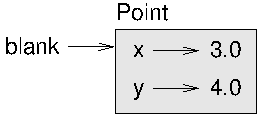
\includegraphics[scale=0.8]{figs/point.pdf}}
 \caption{Διάγραμμα αντικειμένου} 
\label{fig.point}
\end{figure}


 Η μεταβλητή  {\tt blank}  αναφέρεται σε ένα αντικείμενο  Point,  το οποίο περιέχει δύο ιδιότητες. Κάθε ιδιότητα αναφέρεται σε ένα αριθμό κινητής υποδιαστολής.

Μπορείτε να διαβάσετε την τιμή μίας ιδιότητας χρησιμοποιώντας την ίδια σύνταξη :

\begin{verbatim}
>>> print blank.y
4.0
>>> x = blank.x
>>> print x
3.0
\end{verbatim}
%
 Η έκφραση  {\tt blank.x}  σημαίνει : " Πήγαινε στο αντικείμενο στο οποίο αναφέρεται η  {\tt blank}  και 
πάρε την τιμή του  {\tt x}".  Σε αυτήν την περίπτωση, εκχωρούμε αυτήν την τιμή σε μία μεταβλητή με όνομα  {\tt x}.    Δεν υπάρχει καμία σύγκρουση μεταξύ της μεταβλητής  {\tt x}  και της ιδιότητας  {\tt x}.

 Μπορείτε να χρησιμοποιήσετε το συμβολισμό με τελεία σαν μέρος οποιασδήποτε έκφρασης. Για παράδειγμα :

\begin{verbatim}
>>> print '(%g, %g)' % (blank.x, blank.y)
(3.0, 4.0)
>>> distance = math.sqrt(blank.x**2 + blank.y**2)
>>> print distance
5.0
\end{verbatim}
%
 Μπορείτε να περάσετε ένα στιγμιότυπο σαν όρισμα με το γνωστό τρόπο. Για παράδειγμα :
\index{instance!as argument}

\begin{verbatim}
def print_point(p):
    print '(%g, %g)' % (p.x, p.y)
\end{verbatim}
%
 Η  \verb"print_point"  παίρνει ένα  Point  σαν όρισμα και το εμφανίζει με μαθηματικό συμβολισμό.  Για να την δοκιμάσετε, μπορείτε να περάσετε τη  {\tt blank}  σαν όρισμα :

\begin{verbatim}
>>> print_point(blank)
(3.0, 4.0)
\end{verbatim}
%
 Μέσα στη συνάρτηση, η  {\tt p}  είναι ένα ψευδώνυμο για την  {\tt blank}  , άρα αν η συνάρτηση τροποποιήσει την  {\tt p}  αλλάζει και η  {\tt blank}.
\index{aliasing}

\begin{exercise}

Γράψτε μία συνάρτηση με όνομα  \verb"distance_between_points"  η οποία θα παίρνει δύο σημεία σαν ορίσματα 
και θα επιστρέφει την απόσταση μεταξύ τους.
\end{exercise}



\section{Ορθογώνια παραλληλόγραμμα}
\label{rectangles}

Μερικές φορές είναι προφανές ποιες θα πρέπει να είναι οι ιδιότητες ενός αντικειμένου, αλλά κάποιες άλλες όχι. 
Για παράδειγμα, φανταστείτε ότι σχεδιάζετε μία κλάση για να αναπαραστήσετε ορθογώνια παραλληλόγραμμα. Ποιες ιδιότητες 
θα χρησιμοποιούσατε για να καθορίσετε τη θέση και το μέγεθος ενός ορθογωνίου παραλληλογράμμου ;    Για να απλοποιήσουμε τα πράγματα, υποθέστε ότι το παραλληλόγραμμο είναι είτε κάθετο είτε οριζόντιο.
\index{representation}

Υπάρχουν τουλάχιστον δύο ενδεχόμενα :

\begin{itemize}

\item  Μπορείτε να καθορίσετε μία γωνία ή το κέντρο, το πλάτος και το ύψος.

 \item  Μπορείτε να καθορίσετε δύο απέναντι γωνίες.  

\end{itemize}

 Σε αυτό το σημείο είναι δύσκολο να πούμε ποια είναι η καλύτερη επιλογή και έτσι, σαν παράδειγμα, θα υλοποιήσουμε την πρώτη.
\index{Rectangle class}
\index{class!Rectangle}

Αυτός είναι ο ορισμός της κλάσης :

\begin{verbatim}
class Rectangle(object):
    """Represents a rectangle.

    attributes: width, height, corner.
    """
\end{verbatim}
%
 Η συμβολοσειρά τεκμηρίωσης απαριθμεί τις ιδιότητες :  η  {\tt width}  και η  {\tt height}  είναι αριθμοί και  η  {\tt corner}  είναι ένα αντικείμενο  Point  η οποία ορίζει την κάτω-αριστερή γωνία.

Για να αναπαραστήσετε ένα ορθογώνιο παραλληλόγραμμο, πρέπει να δημιουργήσουμε ένα αντικείμενο  Renctangle  και να 
εκχωρήσουμε τιμές στις ιδιότητες :

\begin{verbatim}
box = Rectangle()
box.width = 100.0
box.height = 200.0
box.corner = Point()
box.corner.x = 0.0
box.corner.y = 0.0
\end{verbatim}
%
 Η έκφραση  {\tt box.corner.x}  σημαίνει : " Πήγαινε στο αντικείμενο το οποίο αναφέρεται η  {\tt box}  και επέλεξε την ιδιότητα με όνομα  {\tt corner}  και στη συνέχεια πήγαινε σε αυτό το αντικείμενο και επέλεξε την  {\tt x}".

\begin{figure}
\centerline
{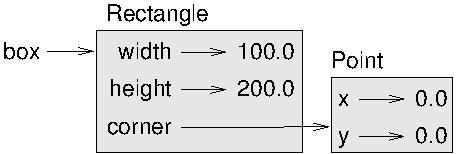
\includegraphics[scale=0.8]{figs/rectangle.pdf}}
 \caption{Διάγραμμα αντικειμένου.} 
\label{fig.rectangle}
\end{figure}


 Η Εικόνα~ \ref{fig.rectangle}  δείχνει την κατάσταση αυτού του αντικειμένου.
\index{state diagram}
\index{diagram!state}
\index{object diagram}
\index{diagram!object}
 Ένα αντικείμενο το οποίο είναι ιδιότητα κάποιου άλλου αντικειμένου είναι ενσωματωμένο.
\index{embedded object}
\index{object!embedded}


\section{Τα στιγμιότυπα σαν επιστρεφόμενες τιμές}
\index{instance!as return value}
\index{return value}

Οι συναρτήσεις μπορούν να επιστρέψουν στιγμιότυπα. Για παράδειγμα, η  \verb"find_center"  παίρνει ένα  {\tt Rectangle}  σαν όρισμα και επιστρέφει ένα  {\tt Point}  το οποίο περιέχει τις συντεταγμένες του κέντρου του ορθογωνίου παραλληλογράμμου :

\begin{verbatim}
def find_center(rect):
    p = Point()
    p.x = rect.corner.x + rect.width/2.0
    p.y = rect.corner.y + rect.height/2.0
    return p
\end{verbatim}
%
 Αυτό είναι ένα παράδειγμα το οποίο περνάει το  {\tt box}  σαν όρισμα και εκχωρεί το σημείο που προκύπτει στην  
{\tt center}:

\begin{verbatim}
>>> center = find_center(box)
>>> print_point(center)
(50.0, 100.0)
\end{verbatim}
%

 
\section{Τα αντικείμενα είναι μεταβλητά}
\index{object!mutable}
\index{mutability}

Μπορείτε να αλλάξετε την κατάσταση ενός αντικειμένου κάνοντας μία εκχώρηση σε μία από τις ιδιότητες του. 
Για παράδειγμα, για να αλλάξετε το μέγεθος ενός ορθογωνίου παραλληλογράμμου χωρίς να αλλάξει η θέση του, μπορείτε να 
τροποποιήσετε την τιμή της  {\tt width}  και της  {\tt height}:

\begin{verbatim}
box.width = box.width + 50
box.height = box.width + 100
\end{verbatim}
%
 Μπορείτε επίσης να γράψετε συναρτήσεις οι οποίες θα τροποποιούν αντικείμενα. Για παράδειγμα, η  \verb"grow_rectangle"  παίρνει ένα  Rectangle  και δύο αριθμούς, το  {\tt dwidth}  και  {\tt dheight},  και προσθέτει τους αριθμούς 
στο πλάτος και το ύψος του ορθογωνίου :

\begin{verbatim}
def grow_rectangle(rect, dwidth, dheight):
    rect.width += dwidth
    rect.height += dheight
\end{verbatim}
%
 Αυτό το παράδειγμα επιδεικνύει το αποτέλεσμα :

\begin{verbatim}
>>> print box.width
100.0
>>> print box.height
200.0
>>> grow_rectangle(box, 50, 100)
>>> print box.width
150.0
>>> print box.height
300.0
\end{verbatim}
%
 Μέσα στη συνάρτηση, το  {\tt rect}  είναι ένα ψευδώνυμο για το  {\tt box},  οπότε αν η συνάρτηση τροποποιήσει το  
{\tt rect},  αλλάζει και το  {\tt box}.

\begin{exercise}

Γράψτε μία συνάρτηση με όνομα  \verb"move_rectangle"  η οποία θα παίρνει ένα  Rectangle  και δύο αριθμούς με ονόματα  {\tt dx}  και  {\tt dy}.   Θα πρέπει να αλλάζει την θέση του ορθογωνίου παραλληλογράμμου προσθέτοντας το  {\tt dx}  στη συντεταγμένη  {\tt x}  του  {\tt corner}  και το  {\tt dy}  στη συντεταγμένη  {\tt y}  του  {\tt corner}. 
\end{exercise}



\section{Αντιγραφή}
\label{copying}
\index{aliasing}

Τα ψευδώνυμα μπορεί να κάνουν ένα πρόγραμμα δύσκολο στην ανάγνωση επειδή οι αλλαγές σε ένα μέρος θα μπορούσαν να έχουν απροσδόκητες συνέπειες σε ένα άλλο μέρος.  Είναι δύσκολο να παρακολουθήσουμε όλες τις μεταβλητές που θα μπορούσαν να αναφέρονται σε ένα συγκεκριμένο αντικείμενο.
\index{copying objects}
\index{object!copying}
\index{copy module}
\index{module!copy}

Συχνά, η αντιγραφή ενός αντικειμένου είναι μία εναλλακτική λύση στην εκχώρηση ψευδωνύμων. Το άρθρωμα  {\tt copy}  περιέχει μία συνάρτηση με όνομα  {\tt copy}  η οποία μπορεί να αντιγράψει οποιοδήποτε αντικείμενο :

\begin{verbatim}
>>> p1 = Point()
>>> p1.x = 3.0
>>> p1.y = 4.0

>>> import copy
>>> p2 = copy.copy(p1)
\end{verbatim}
%
 Το  {\tt p1}  και το  {\tt p2}  περιέχουν τα ίδια δεδομένα, αλλά είναι δύο διαφορετικά σημεία.  

\begin{verbatim}
>>> print_point(p1)
(3.0, 4.0)
>>> print_point(p2)
(3.0, 4.0)
>>> p1 is p2
False
>>> p1 == p2
False
\end{verbatim}
%
 Ο τελεστής  {\tt is}  υποδεικνύει αυτό που περιμέναμε, ότι δηλαδή το  {\tt p1}  και το  {\tt p2}   δεν είναι το ίδιο αντικείμενο. Αλλά ίσως περιμένατε ότι ο τελεστής  {\tt ==}  θα απέδιδε  {\tt True}  αφού αυτά τα σημεία περιέχουν τα ίδια δεδομένα. Σε αυτήν την περίπτωση, θα απογοητευθείτε, αφού για τα στιγμιότυπα η προεπιλεγμένη συμπεριφορά του τελεστή  {\tt ==}  είναι η ίδια με αυτήν του τελεστή  {\tt is}.  
Και οι δύο, ελέγχουν την ταυτότητα των αντικειμένων και όχι την ισοδυναμία τους. Αυτή η συμπεριφορά μπορεί να αλλάξει, θα δούμε πως αργότερα.
\index{is operator}
\index{operator!is}

Αν χρησιμοποιήσετε την  {\tt copy.copy}  για να αντιγράψετε ένα ορθογώνιο παραλληλόγραμμο, θα δείτε ότι αντιγράφει το αντικείμενο  Rectangle  αλλά όχι το ενσωματωμένο σημείο. 
\index{embedded object!copying}

\begin{verbatim}
>>> box2 = copy.copy(box)
>>> box2 is box
False
>>> box2.corner is box.corner
True
\end{verbatim}

\begin{figure}
\centerline
{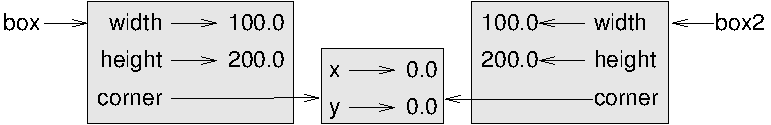
\includegraphics[scale=0.8]{figs/rectangle2.pdf}}
 \caption{Διάγραμμα αντικειμένων.} 
\label{fig.rectangle2}
\end{figure}

 Η Εικόνα~ \ref{fig.rectangle2}  δείχνει πως είναι το διάγραμμα αντικειμένων.
\index{state diagram}
\index{diagram!state}
\index{object diagram}
\index{diagram!object}

 Αυτή η διαδικασία ονομάζεται {\bf ρηχή αντιγραφή} επειδή αντιγράφει το αντικείμενο και όλες τις αναφορές που περιέχει, 
αλλά όχι τα ενσωματωμένα αντικείμενα.
\index{shallow copy}
\index{copy!shallow}

Στις περισσότερες εφαρμογές όμως, αυτό δεν το θέλετε.  Σε αυτό το παράδειγμα, η επίκληση της  \verb"grow_rectangle"  σε 
ένα από τα ορθογώνια παραλληλόγραμμα δεν θα επηρέαζε το άλλο, αλλά η επίκληση της  \verb"move_rectangle"  σε ένα οποιοδήποτε 
θα επηρέαζε και τα δύο. Αυτή η συμπεριφορά προκαλεί σύγχυση και είναι επιρρεπή σε λάθη.
\index{deep copy}
\index{copy!deep}

Ευτυχώς, το άρθρωμα  {\tt copy}  περιέχει μία μέθοδο με όνομα  {\tt deepcopy}  η οποία δεν αντιγράφει μόνο το αντικείμενο αλλά και τα αντικείμενα στα οποία αναφέρεται, τα αντικείμενα στα οποία αναφέρονται αυτά και ούτω καθεξής.
Όπως θα περιμένατε, αυτή η διαδικασία ονομάζεται βαθιά αντιγραφή. 
\index{deepcopy function}
\index{function!deepcopy}

\begin{verbatim}
>>> box3 = copy.deepcopy(box)
>>> box3 is box
False
>>> box3.corner is box.corner
False
\end{verbatim}
%
 Το  {\tt box3}  και το  {\tt box}  είναι δύο τελείως διαφορετικά αντικείμενα.


\begin{exercise}

Γράψτε μία έκδοση της  \verb"move_rectangle"  η οποία θα δημιουργεί και θα επιστρέφει ένα νέο  Rectangle  
αντί να τροποποιεί το παλιό.
\end{exercise}



\section{Αποσφαλμάτωση}
\label{hasattr}
\index{debugging}

Όταν αρχίσετε να δουλεύετε με αντικείμενα, είναι πιθανό να αντιμετωπίσετε κάποιες νέες εξαιρέσεις. Αν δοκιμάσετε να αποκτήσετε πρόσβαση σε μία ιδιότητα η οποία δεν υπάρχει θα πάρετε 
ένα  {\tt AttributeError}:
\index{exception!AttributeError}
\index{AttributeError}

\begin{verbatim}
>>> p = Point()
>>> print p.z
AttributeError: Point instance has no attribute 'z'
\end{verbatim}
%
 Αν δεν είστε σίγουροι για τον τύπο του αντικειμένου μπορείτε να ρωτήσετε :
\index{type function}
\index{function!type}

\begin{verbatim}
>>> type(p)
<type '__main__.Point'>
\end{verbatim}
%
 Αν δεν είστε σίγουροι για το αν ένα αντικείμενο έχει μία συγκεκριμένη ιδιότητα, 
μπορείτε να χρησιμοποιήσετε την ενσωματωμένη συνάρτηση  {\tt hasattr}:
\index{hasattr function}
\index{function!hasattr}

\begin{verbatim}
>>> hasattr(p, 'x')
True
>>> hasattr(p, 'z')
False
\end{verbatim}
%
 Το πρώτο όρισμα μπορεί να είναι ένα οποιοδήποτε αντικείμενο και το δεύτερο είναι μία 
συμβολοσειρά η οποία περιέχει το όνομα της ιδιότητας.



\section{Ορολογία}

\begin{description}

\item[κλάση:] Ένας τύπος ορισμένος από το χρήστη.  Ο ορισμός μίας κλάσης δημιουργεί ένα νέο  αντικείμενο κλάσης.
\index{class}

\item[αντικείμενο κλάσης:]  Ένα αντικείμενο το οποίο περιέχει πληροφορίες σχετικά με έναν τύπο ορισμένο από το χρήστη.  Το αντικείμενο της κλάσης μπορεί να χρησιμοποιηθεί για να δημιουργηθούν στιγμιότυπα αυτού του τύπου.
\index{class object}
\index{object!class}

\item[στιγμιότυπο:] Ένα αντικείμενο το οποίο ανήκει σε μία κλάση.
\index{instance}

\item[ιδιότητα:] Μία από τις μεταβλητές που σχετίζονται με ένα αντικείμενο.
\index{attribute!instance}
\index{instance attribute}

\item[ενσωματωμένο αντικείμενο:] Ένα αντικείμενο το οποίο αποθηκεύεται σαν ιδιότητα ενός 
άλλου αντικειμένου.
\index{embedded object}
\index{object!embedded}

\item[ρηχή αντιγραφή:] Η αντιγραφή των περιεχομένων ενός αντικειμένου, συμπεριλαμβανομένων και των αναφορών στα ενσωματωμένα αντικείμενα.  Υλοποιείται με τη συνάρτηση  {\tt copy}  του 
αρθρώματος  {\tt copy}.
\index{shallow copy}

\item[βαθιά αντιγραφή:] Η αντιγραφή των περιεχομένων ενός αντικειμένου καθώς επίσης και των  ενσωματωμένων αντικειμένων, και των αντικειμένων που είναι ενσωματωμένα σε αυτά και ούτω καθεξής.  Υλοποιείται από τη συνάρτηση  {\tt deepcopy}  του αρθρώματος  {\tt copy}. 
\index{deep copy}

\item[διάγραμμα αντικειμένων:] Ένα διάγραμμα το οποίο δείχνει τα αντικείμενα, τις ιδιότητές τους και τις τιμές των ιδιοτήτων.
\index{object diagram}
\index{diagram!object}

\end{description}


\section{Ασκήσεις}

\begin{exercise}
\label{canvas} 
\index{Swampy}
\index{World module}
\index{module!World}

Το πακέτο  Swampy  (βλ. Κεφάλαιο~ \ref{turtlechap} ) παρέχει ένα άρθρωμα με όνομα 
 {\tt World},  το οποίο ορίζει έναν τύπο ορισμένο από το χρήστη, το όνομα του οποίου είναι επίσης  {\tt World}.  
Μπορείτε να τον εισάγετε έτσι :

\begin{verbatim}
from swampy.World import World
\end{verbatim}

 Ή, ανάλογα με το πως εγκαταστήσατε το  Swampy,  έτσι :

\begin{verbatim}
from World import World
\end{verbatim}

 Ο ακόλουθος κώδικας δημιουργεί ένα αντικείμενο  World  και καλεί τη μέθοδο  
{\tt mainloop}  , η οποία περιμένει το χρήστη. 

\begin{verbatim}
world = World()
world.mainloop()
\end{verbatim}

 Θα πρέπει να εμφανιστεί ένα παράθυρο με μία γραμμή τίτλου και ένα άδειο τετράγωνο. 
Θα χρησιμοποιήσουμε αυτό το παράθυρο για να σχεδιάσουμε σημεία  (Points),  ορθογώνια 
παραλληλόγραμμα  (Rectanlges)  και άλλα σχήματα. 
Προσθέστε τις παρακάτω γραμμές προτού καλέσετε την  \verb"mainloop"  και ξανατρέξτε το 
πρόγραμμα. 
\index{Canvas object}
\index{object!Canvas}

\begin{verbatim}
canvas = world.ca(width=500, height=500, background='white')
bbox = [[-150,-100], [150, 100]]
canvas.rectangle(bbox, outline='black', width=2, fill='green4')
\end{verbatim}

 Θα πρέπει να δείτε ένα πράσινο ορθογώνιο παραλληλόγραμμο με μαύρο περίγραμμα.  
Η πρώτη γραμμή δημιουργεί έναν καμβά, ο οποίος εμφανίζεται στο παράθυρο σαν ένα λευκό τετράγωνο.  
Το αντικείμενο  Canvas  παρέχει μεθόδους όπως η  {\tt rectangle}  για το σχεδιασμό διαφόρων σχημάτων.  
\index{bounding box}

Η  {\tt bbox}  είναι μία λίστα από λίστες η οποία αναπαριστά το  " πλαίσιο οριοθέτησης "  του 
ορθογωνίου παραλληλογράμμου.  Το πρώτο ζευγάρι συντεταγμένων είναι η κάτω-αριστερή γωνία του ορθογωνίου και το δεύτερο 
ζευγάρι είναι η πάνω-δεξιά γωνία.  

Μπορείτε να σχεδιάσετε ένα κύκλο κάπως έτσι : 

\begin{verbatim}
canvas.circle([-25,0], 70, outline=None, fill='red')
\end{verbatim}

 Η πρώτη παράμετρος είναι το ζευγάρι συντεταγμένων για το κέντρο του κύκλου και η δεύτερη είναι η ακτίνα.  

Αν προσθέσετε αυτή τη γραμμή στο πρόγραμμα, το αποτέλεσμα θα πρέπει να μοιάζει με την σημαία του Μπανγκλαντές 
(βλ.  \url{http://en.wikipedia.org/wiki/Gallery_of_sovereign-state_flags} ).
\index{Bangladesh, national flag}


\begin{enumerate}

\item Γράψτε μία συνάρτηση με όνομα  \verb"draw_rectangle"  η οποία θα παίρνει ένα αντικείμενο  Canvas  και 
  και ένα  Rectangle  σαν ορίσματα και θα σχεδιάζει μία αναπαράσταση του  Rectangle  στο  Canvas. 
   
\item Προσθέστε μία ιδιότητα με όνομα  {\tt color}  στα αντικείμενα  Rectangle  και τροποποιήστε την  
  \verb"draw_rectangle"  έτσι ώστε να χρησιμοποιεί αυτήν την ιδιότητα σαν χρώμα γεμίσματος.
  
\item Γράψτε μία συνάρτηση με όνομα  \verb"draw_point"  η οποία θα παίρνει ένα αντικείμενο  Canvas  και ένα 
    Point  σαν ορίσματα και θα σχεδιάζει μία αναπαράσταση του  Point  στο  Canvas.  

\item Ορίστε μία νέα κλάση με όνομα  Circle  με τις κατάλληλες ιδιότητες και δημιουργήστε μερικά αντικείμενα  Circle.   
  Γράψτε μία συνάρτηση με όνομα  \verb"draw_circle"  η οποία θα σχεδιάζει κύκλους στον καμβά.
\index{Czech Republic, national flag}

\item Γράψτε ένα πρόγραμμα το οποίο θα σχεδιάζει τη σημαία της Τσεχίας.  
  Σημείωση :  μπορείτε να σχεδιάσετε ένα πολύγωνο κάπως έτσι :

\begin{verbatim}
points = [[-150,-100], [150, 100], [150, -100]]
canvas.polygon(points, fill='blue')
\end{verbatim}

\end{enumerate}
\index{color list}
\index{available colors}

 Έχω γράψει ένα μικρό πρόγραμμα το οποίο απαριθμεί τα διαθέσιμα χρώματα.  Μπορείτε να το κατεβάσετε από εδώ : 
\url{http://thinkpython.com/code/color_list.py}. 

\end{exercise}


\chapter{Κλάσεις και συναρτήσεις}
\label{time}

Τα παραδείγματα αυτού του κεφαλαίου είναι διαθέσιμα στο σύνδεσμο :
\url{http://thinkpython.com/code/Time1.py}.

 
\section{Ώρα}
\label{time.object}

Σαν ένα ακόμα παράδειγμα τύπου οριζόμενο από το χρήστη, θα ορίσουμε μία κλάση με όνομα  {\tt Time}  η οποία 
θα καταγράφει την ώρα της ημέρας. Ο ορισμός της κλάσης είναι ο εξής : 
\index{user-defined type}
\index{type!user-defined}
\index{Time class}
\index{class!Time}

\begin{verbatim}
class Time(object):
    """Represents the time of day.

    attributes: hour, minute, second
    """
\end{verbatim}
%
 Μπορούμε να δημιουργήσουμε ένα νέο αντικείμενο  {\tt Time}  και να εκχωρήσουμε ιδιότητες για τις ώρες, τα λεπτά 
και τα δευτερόλεπτα :

\begin{verbatim}
time = Time()
time.hour = 11
time.minute = 59
time.second = 30
\end{verbatim}
%
 Το διάγραμμα κατάστασης για το αντικείμενο  {\tt Time}  είναι όπως αυτό στην Εικόνα~ \ref{fig.time}.
\index{state diagram}
\index{diagram!state}
\index{object diagram}
\index{diagram!object}

 
\begin{exercise}
\label{ex.printtime}

Γράψτε μία συνάρτηση με όνομα  \verb"print_time"  η οποία θα παίρνει ένα αντικείμενο  Time  και θα το εμφανίζει στη 
μορφή  {\tt hour:minute:second}.   
Σημείωση :  η ακολουθία διαμόρφωσης  \verb"'%.2d'"  εμφανίζει έναν ακέραιο χρησιμοποιώντας τουλάχιστον δύο ψηφία, 
συμπεριλαμβανομένου και ενός μηδενικού στην αρχή αν είναι απαραίτητο.
\end{exercise}

\begin{exercise}
\label{isafter}
\index{boolean function}

Γράψτε μία λογική συνάρτηση με όνομα  \verb"is_after"  η οποία θα παίρνει δύο αντικείμενα  Time,  το  {\tt t1}  
και το  {\tt t2},  και θα επιστρέφει  {\tt True}  αν το  {\tt t1}  ακολουθεί το  {\tt t2}  χρονολογικά και 
 {\tt False}  αλλιώς. Πρόκληση :  μην χρησιμοποιήσετε τη δήλωση  {\tt if}.
\end{exercise}

\begin{figure}
\centerline
{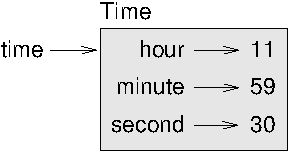
\includegraphics[scale=0.8]{figs/time.pdf}}
 \caption{Διάγραμμα αντικειμένου.}  
\label{fig.time}
\end{figure}


 
\section{Αγνές συναρτήσεις}
\index{prototype and patch}
\index{development plan!prototype and patch}

Στις επόμενες ενότητες, θα γράψουμε δύο συναρτήσεις οι οποίες θα προσθέτουν τιμές ώρας.  Αυτές επιδεικνύουν δύο είδη συναρτήσεων :  τις αγνές συναρτήσεις και τις συναρτήσεις τροποποίησης.  Επίσης, επιδεικνύουν και ένα πλάνο ανάπτυξης, το οποίο αποκαλώ  " πρωτότυπο και επιδιόρθωση ",  το οποίο αποτελεί ένα τρόπο αντιμετώπισης ενός σύνθετου προβλήματος ξεκινώντας με ένα απλό πρωτότυπο και αντιμετωπίζοντας σταδιακά την πολυπλοκότητα.

Αυτό είναι ένα απλό πρωτότυπο της  \verb"add_time":

\begin{verbatim}
def add_time(t1, t2):
    sum = Time()
    sum.hour = t1.hour + t2.hour
    sum.minute = t1.minute + t2.minute
    sum.second = t1.second + t2.second
    return sum
\end{verbatim}
%
 Η συνάρτηση δημιουργεί ένα νέο αντικείμενο  {\tt Time},  αρχικοποιεί τις ιδιότητές του και επιστρέφει μία αναφορά 
σε ένα νέο αντικείμενο.  Αυτή ονομάζεται αγνή συνάρτηση επειδή δεν τροποποιεί κανένα από τα αντικείμενα που της περάστηκαν σαν 
ορίσματα και δεν έχει και καμία επίδραση, όπως να εμφανίζει μία τιμή ή να δέχεται είσοδο από το χρήστη, εκτός από την επιστρεφόμενη 
τιμή.
\index{pure function}
\index{function type!pure}

Για να δοκιμάσουμε αυτήν τη συνάρτηση, θα δημιουργήσω δύο αντικείμενα  Time:  το  {\tt start}  περιέχει την ώρα έναρξης 
μιας ταινίας, όπως η  {\em Monty Python and the Holy Grail},  και το  {\tt duration}  περιέχει την διάρκεια της ταινίας, η οποία είναι μία ώρα και 35 λεπτά.
\index{Monty Python and the Holy Grail}

Η  \verb"add_time"  υπολογίζει πότε θα τελειώσει η ταινία :

\begin{verbatim}
>>> start = Time()
>>> start.hour = 9
>>> start.minute = 45
>>> start.second =  0

>>> duration = Time()
>>> duration.hour = 1
>>> duration.minute = 35
>>> duration.second = 0

>>> done = add_time(start, duration)
>>> print_time(done)
10:80:00
\end{verbatim}
%
 Το αποτέλεσμα,  {\tt 10:80:00},  ίσως να μην είναι αυτό που θα περιμένατε.  Το πρόβλημα έγκειται στο ότι αυτή η συνάρτηση 
δεν χειρίζεται τις περιπτώσεις όπου ο αριθμός των δευτερολέπτων ή των λεπτών γίνεται μεγαλύτερος από εξήντα.  Όταν συμβαίνει αυτό, θα πρέπει να  " μεταφέρουμε "  τα έξτρα δευτερόλεπτα στη στήλη των λεπτών ή τα έξτρα λεπτά στη στήλη της ωρών.
\index{carrying, addition with}

Αυτή είναι μία βελτιωμένη έκδοση :

\begin{verbatim}
def add_time(t1, t2):
    sum = Time()
    sum.hour = t1.hour + t2.hour
    sum.minute = t1.minute + t2.minute
    sum.second = t1.second + t2.second

    if sum.second >= 60:
        sum.second -= 60
        sum.minute += 1

    if sum.minute >= 60:
        sum.minute -= 60
        sum.hour += 1

    return sum
\end{verbatim}
%
 Παρόλο που αυτή η συνάρτηση είναι σωστή, αρχίζει να γίνεται μεγάλη.  Θα δούμε μία άλλη εναλλακτική λύση 
αργότερα.



\section{Συναρτήσεις τροποποίησης}
\label{increment}
\index{modifier}
\index{function type!modifier}

Μερικές φορές είναι χρήσιμο μια συνάρτηση να τροποποιεί τα αντικείμενα που παίρνει σαν παραμέτρους.  Σε αυτήν την περίπτωση, οι αλλαγές είναι ορατές στον καλούντα.  Οι συναρτήσεις που δουλεύουν κατ' αυτόν τον τρόπο ονομάζονται  " συναρτήσεις τροποποίησης ".  
\index{increment}

Η  {\tt increment},  η οποία προσθέτει ένα δεδομένο αριθμό δευτερολέπτων σε ένα αντικείμενο  {\tt Time},  μπορεί να γραφτεί φυσικά σαν μία συνάρτηση τροποποίησης.  Αυτό είναι ένα προσχέδιο :

\begin{verbatim}
def increment(time, seconds):
    time.second += seconds

    if time.second >= 60:
        time.second -= 60
        time.minute += 1

    if time.minute >= 60:
        time.minute -= 60
        time.hour += 1
\end{verbatim}
%
 Η πρώτη γραμμή εκτελεί τη βασική λειτουργία και το υπόλοιπο διαχειρίζεται τις ειδικές περιπτώσεις που είδαμε νωρίτερα.
\index{special case}

Είναι σωστή αυτή η συνάρτηση ;   Τι συμβαίνει αν η παράμετρος  {\tt seconds}  είναι πολύ μεγαλύτερη από εξήντα ;

 Σε αυτήν την περίπτωση δεν είναι αρκετό να μεταφέρουμε μία φορά, πρέπει να συνεχίσουμε μέχρι η  {\tt time.second}  να 
γίνει μικρότερη από εξήντα.  Μία λύση είναι να αντικαταστήσουμε τις δηλώσεις  {\tt if}  με δηλώσεις  {\tt while}.   Αυτό θα κάνει την συνάρτηση σωστή αλλά όχι και πολύ αποδοτική.

\begin{exercise}

Γράψτε μία σωστή έκδοση της  {\tt increment}  η οποία δεν θα περιέχει κανένα βρόχο.

Οτιδήποτε μπορεί να υλοποιηθεί με συναρτήσεις τροποποίησης μπορεί επίσης να υλοποιηθεί και με αγνές συναρτήσεις.  Στην πραγματικότητα, μερικές γλώσσες προγραμματισμού επιτρέπουν μόνο αγνές συναρτήσεις.  Υπάρχουν κάποιες ενδείξεις ότι τα προγράμματα που χρησιμοποιούν αγνές συναρτήσεις είναι πιο γρήγορα στην ανάπτυξη και λιγότερο επιρρεπή στα λάθη σε σχέση με τα προγράμματα που χρησιμοποιούν συναρτήσεις τροποποίησης.  Αλλά, μερικές φορές, οι συναρτήσεις τροποποίησης είναι πολύ βολικές και λειτουργικά προγράμματα έχουν την τάση να είναι λιγότερο αποδοτικά.

Σε γενικές γραμμές, συνιστώ να γράφετε αγνές συναρτήσεις όπου είναι λογικό και να καταφεύγετε στις συναρτήσεις τροποποίησης μόνο όταν υπάρχει σημαντικό πλεονέκτημα.  Αυτή η προσέγγιση μπορεί να χαρακτηριστεί ως  " συναρτησιακό ύφος  προγραμματισμού ".  
\end{exercise}
\index{functional programming style}


\begin{exercise}

Γράψτε μία  "αγνή"  έκδοση της  {\tt increment}  η οποία θα δημιουργεί και θα επιστρέφει ένα νέο 
αντικείμενο  Time  αντί να τροποποιεί την παράμετρο.
\end{exercise}


\section{Πρωτοτυποποίηση εναντίον σχεδιασμού}
\label{prototype}
\index{prototype and patch}
\index{development plan!prototype and patch}
\index{planned development}
\index{development plan!planned}

Το πλάνο ανάπτυξης το οποίο επιδεικνύω ονομάζεται  " πρωτότυπο και ενημέρωση ".   Για κάθε συνάρτηση, έγραφα ένα πρωτότυπο το οποίο εκτελούσε το βασικό υπολογισμό και στη συνέχεια το δοκίμαζα, διορθώνοντας λάθη στην πορεία.

Αυτή η προσέγγιση μπορεί να είναι αποτελεσματική, ειδικά αν δεν έχετε κατανοήσει καλά το πρόβλημα εξαρχής.  Αλλά η σταδιακή ενημέρωση μπορεί να δημιουργήσει κώδικα ο οποίος θα είναι ασκόπως περίπλοκος (αφού θα εξετάζει πολλές ειδικές περιπτώσεις) και αναξιόπιστος (από τη στιγμή που είναι δύσκολο να γνωρίζετε αν πρέπει να βρείτε όλα τα σφάλματα).

Μία εναλλακτική λύση είναι η ανάπτυξη βάση σχεδίου, κατά την οποία η υψηλού επιπέδου 
επίγνωση του προβλήματος μπορεί να κάνει τον προγραμματισμό ευκολότερο.  Σε αυτήν την περίπτωση, η επίγνωση έγκειται στο ότι το αντικείμενο  Time  είναι ένας τριψήφιος αριθμός στη βάση του 60  ( βλ.  \url{http://en.wikipedia.org/wiki/Sexagesimal})!   Η ιδιότητα  {\tt second}  είναι η  " στήλη των μονάδων ",  η ιδιότητα  {\tt minute}  είναι η  " στήλη των εξήντα "  και η ιδιότητα  {\tt hour}  είναι η  " η στήλη των τριάντα έξι εκατοντάδων ". 
\index{sexagesimal}

 Όταν γράψαμε την  \verb"add_time"  και την  {\tt increment},  ουσιαστικά κάναμε πρόσθεση στην βάση του 60, αυτός είναι και ο λόγος που έπρεπε να κάνουμε μεταφορά από τη μία στήλη στην επόμενη. 
\index{carrying, addition with}

Αυτή η διαπίστωση μας υποδεικνύει μία άλλη προσέγγιση του όλου προβλήματος.  Μπορούμε να μετατρέψουμε τα αντικείμενα  Time  σε ακέραιους αριθμούς και να επωφεληθούμε από το γεγονός ότι ο υπολογιστής ξέρει να κάνει αριθμητική ακεραίων.

Αυτή είναι μία συνάρτηση η οποία μετατρέπει αντικείμενα  Time  σε ακέραιους :

\begin{verbatim}
def time_to_int(time):
    minutes = time.hour * 60 + time.minute
    seconds = minutes * 60 + time.second
    return seconds
\end{verbatim}
%
 Και αυτή είναι η συνάρτηση που μετατρέπει τους ακέραιους σε αντικείμενα  Time  (θυμηθείτε ότι η  {\tt divmod}  διαιρεί το πρώτο όρισμα με το δεύτερο και επιστρέφει το πηλίκο και το υπόλοιπο σαν μία πλειάδα). 
\index{divmod}

\begin{verbatim}
def int_to_time(seconds):
    time = Time()
    minutes, time.second = divmod(seconds, 60)
    time.hour, time.minute = divmod(minutes, 60)
    return time
\end{verbatim}
%
 Ίσως πρέπει να σκεφτείτε λίγο και να τρέξετε μερικά παραδείγματα, ούτως ώστε να πειστείτε ότι αυτές οι συναρτήσεις είναι σωστές.  Ένας τρόπος για να τις δοκιμάσετε είναι να τσεκάρετε ότι  \verb"time_to_int(int_to_time(x)) == x"  για διάφορες τιμές της  {\tt x}.  Αυτό είναι ένα παράδειγμα ενός ελέγχου συνέπειας.
\index{consistency check}

Αφού πειστείτε ότι είναι σωστές, μπορείτε να τις χρησιμοποιήσετε για να ξαναγράψετε την  
\verb"add_time":

\begin{verbatim}
def add_time(t1, t2):
    seconds = time_to_int(t1) + time_to_int(t2)
    return int_to_time(seconds)
\end{verbatim}
%
 Αυτή η έκδοση είναι μικρότερη από την αρχική και ευκολότερη στην επαλήθευση

\begin{exercise}

Ξαναγράψτε την  {\tt increment}  χρησιμοποιώντας τις  \verb"time_to_int"  και  \verb"int_to_time".
\end{exercise}

Σε μερικές περιπτώσεις, η μετατροπή από τη βάση του 60 στη βάση του 10 και πίσω είναι δυσκολότερη σε σχέση με τον χειρισμό 
ωρών.  Η μετατροπή βάσης είναι κάπως αφηρημένη διαδικασία σε σχέση με τον απλό χειρισμό των τιμών ώρας.

Αλλά αν έχουμε την διορατικότητα να μεταχειριστούμε τις ώρες στη βάση του 60 και επενδύσουμε στο γράψιμο των συναρτήσεων 
μετατροπής  (\verb"time_to_int"  και  \verb"int_to_time"),  τότε θα πάρουμε ένα πρόγραμμα το οποίο θα είναι μικρότερο, ευκολότερο στο διάβασμα και την αποσφαλμάτωση και πιο αξιόπιστο.

Επίσης είναι ευκολότερο να προσθέτουμε λειτουργίες εκ των υστέρων.  Για παράδειγμα, φανταστείτε να αφαιρούσατε δύο αντικείμενα  Time  για να βρείτε τη διάρκεια μεταξύ τους. Η αφελής προσέγγιση θα ήταν να υλοποιούσαμε αφαίρεση με δανεισμό. Χρησιμοποιώντας τις συναρτήσεις μετατροπής θα ήταν ευκολότερο και ορθότερο.
\index{subtraction with borrowing}
\index{borrowing, subtraction with}
\index{generalization}

Μερικές φορές, κατά ειρωνικό τρόπο, το να κάνουμε ένα πρόβλημα δυσκολότερο (ή πιο γενικό) το κάνει ευκολότερο (επειδή υπάρχουν λιγότερες ειδικές περιπτώσεις και λιγότερες πιθανότητες για σφάλματα).



\section{Αποσφαλμάτωση}
\index{debugging}

Ένα αντικείμενο  Time  είναι καλά διαμορφωμένο αν οι τιμές της  {\tt minute}  και της  {\tt second}  είναι 
μεταξύ του 0 και του 60 (συμπεριλαμβανομένου του 0 αλλά όχι του 60) και αν η  {\tt hour}  είναι θετική.  Η  {\tt hour}  και η  {\tt minute}  θα πρέπει να είναι ακέραιες τιμές, αλλά η θα μπορούσε να έχει ένα κλασματικό μέρος.
\index{invariant}

Αυτού του είδους οι απαιτήσεις ονομάζονται  " αμετάβλητες "  επειδή πρέπει να είναι πάντα αληθείς.  Για να το θέσουμε διαφορετικά, αν δεν είναι αληθείς, τότε κάτι πήγε στραβά.

Το γράψιμο κώδικα για τον έλεγχο των αμετάβλητων συνθηκών μπορεί να σας βοηθήσει να εντοπίσετε λάθη και να βρείτε τις αιτίες 
τους.  Για παράδειγμα, μπορεί να έχετε μία συνάρτηση όπως η  \verb"valid_time"  η οποία παίρνει ένα αντικείμενο  Time  και επιστρέφει  {\tt False}  αν παραβιάζεται μία αμετάβλητη συνθήκη :

\begin{verbatim}
def valid_time(time):
    if time.hour < 0 or time.minute < 0 or time.second < 0:
        return False
    if time.minute >= 60 or time.second >= 60:
        return False
    return True
\end{verbatim}
%
 Στην συνέχεια, στην αρχή κάθε συνάρτησης, μπορείτε να ελέγξετε τα ορίσματα για να σιγουρευτείτε ότι είναι έγκυρα :
\index{raise statement}
\index{statement!raise}

\begin{verbatim}
def add_time(t1, t2):
    if not valid_time(t1) or not valid_time(t2):
        raise ValueError, 'invalid Time object in add_time'
    seconds = time_to_int(t1) + time_to_int(t2)
    return int_to_time(seconds)
\end{verbatim}
%
 Ή μπορείτε να χρησιμοποιήσετε μία δήλωση  {\tt assert},  η οποία ελέγχει μία δεδομένη σταθερά και εγείρει μία 
εξαίρεση αν αποτύχει :
\index{assert statement}
\index{statement!assert}

\begin{verbatim}
def add_time(t1, t2):
    assert valid_time(t1) and valid_time(t2)
    seconds = time_to_int(t1) + time_to_int(t2)
    return int_to_time(seconds)
\end{verbatim}
%
 Οι δηλώσεις  {\tt assert}  είναι χρήσιμες επειδή ξεχωρίζουν τον κώδικα που ασχολείται με τις κανονικές συνθήκες 
από τον κώδικα που ελέγχει για σφάλματα.


\section{Ορολογία}

\begin{description}

\item[πρωτότυπο και ενημέρωση:] Ένα πλάνο ανάπτυξης το οποίο περιλαμβάνει το γράψιμο ενός προσχεδίου του προγράμματος, τις δοκιμές και τη διόρθωση σφαλμάτων όταν και αν εντοπιστούν.
\index{prototype and patch}

\item[ανάπτυξη βάση σχεδίου:] Ένα πλάνο ανάπτυξης το οποίο περιλαμβάνει υψηλού επιπέδου επίγνωση του προβλήματος και 
περισσότερο σχεδιασμό σε σχέση με τη σταδιακή ανάπτυξη ή ανάπτυξη βάση πρωτότυπου.
\index{planned development}

\item[αγνή συνάρτηση:] Μία συνάρτηση η οποία δεν τροποποιεί κανένα από τα αντικείμενα που δέχεται σαν ορίσματα.  Οι περισσότερες αγνές συναρτήσεις είναι γόνιμες.
\index{pure function}

\item[συνάρτηση τροποποίησης:] Μία συνάρτηση η οποία μεταβάλλει ένα ή περισσότερα από τα αντικείμενα που δέχεται σαν ορίσματα.   
Οι περισσότερες συναρτήσεις τροποποίησης είναι άκαρπες.
\index{modifier}

\item[συναρτησιακό ύφος προγραμματισμού:] Ένα ύφος σχεδίασης προγράμματος στο οποίο η πλειονότητα των συναρτήσεων είναι αγνές.
\index{functional programming style}

\item[σταθερή:] Μία συνθήκη η οποία θα πρέπει να είναι συνεχώς αληθής κατά την εκτέλεση ενός προγράμματος.
\index{invariant}

\end{description}


\section{Ασκήσεις}

Τα παραδείγματα κώδικα αυτού του κεφαλαίου είναι διαθέσιμα στο σύνδεσμο 
\url{http://thinkpython.com/code/Time1.py}  και οι λύσεις αυτών των ασκήσεων στο 
σύνδεσμο  \url{http://thinkpython.com/code/Time1_soln.py}.

\begin{exercise}

Γράψτε μία συνάρτηση με όνομα  \verb"mul_time"  η οποία θα παίρνει ένα αντικείμενο 
 Time  και έναν αριθμό και θα επιστρέφει ένα νέο αντικείμενο  Time  το οποίο 
θα περιέχει το γινόμενο του αρχικού αντικειμένου και του αριθμού.

Στη συνέχεια χρησιμοποιήστε την  \verb"mul_time"  για να γράψετε μία συνάρτηση η 
οποία θα παίρνει ένα αντικείμενο  Time  το οποίο θα αντιπροσωπεύει το χρόνο τερματισμού ενός αγώνα και έναν αριθμό ο οποίος θα αντιπροσωπεύει την απόσταση, και θα 
επιστρέφει ένα αντικείμενο  Time  το οποίο θα αντιπροσωπεύει το μέσο ρυθμό (χρόνος ανά μίλι).
\index{running pace}

\end{exercise}

%\begin{exercise}
%\index{Date class}
%\index{class!Date}

%Write a class definition for a Date object that has attributes {\tt
%  day}, {\tt month} and {\tt year}.  Write a function called
%\verb"increment_date" that takes a Date object, {\tt date} and an
%integer, {\tt n}, and returns a new Date object that
%represents the day {\tt n} days after {\tt date}.  Hint:
%``Thirty days hath September...''  Challenge: does your function
%deal with leap years correctly?  See \url{http://en.wikipedia.org/wiki/Leap_year}.

%\end{exercise}


\begin{exercise}
\index{datetime module}
\index{module!datetime}

Το άρθρωμα  {\tt datetime}  παρέχει τα αντικείμενα  {\tt date}  και  {\tt time}  τα οποία είναι παρόμοια με τα  Date  και  Time  αυτού του κεφαλαίου με τη διαφορά ότι παρέχουν ένα ευρύ σύνολο μεθόδων και τελεστών. Διαβάστε την τεκμηρίωση στο σύνδεσμο \url{http://docs.python.org/2/library/datetime.html}. 

\begin{enumerate}

\item Χρησιμοποιήστε το άρθρωμα  {\tt datetime}  για να γράψετε ένα πρόγραμμα το 
  οποίο θα παίρνει την τρέχουσα ημερομηνία και θα εμφανίζει τη μέρα της εβδομάδας
\index{birthday}

\item Γράψτε ένα πρόγραμμα το οποίο θα παίρνει σαν είσοδο μία ημερομηνία γέννησης 
  και θα εμφανίζει την ηλικία του χρήστη και τον αριθμό των ημερών, ωρών, λεπτών και 
  δευτερολέπτων μέχρι την επόμενη ημέρα γενεθλίων.

\item Για δύο άτομα που έχουν γεννηθεί σε διαφορετικές ημερομηνίες, υπάρχει μία ημέρα στην  
  οποία ο ένας είναι δύο φορές μεγαλύτερος από τον άλλο. Αυτή είναι η  " Διπλή τους 
  Μέρα ".   Γράψτε ένα πρόγραμμα το οποίο θα παίρνει δύο ημερομηνίες γέννησης και θα 
  υπολογίζει την Διπλή τους Μέρα.

\item Για μεγαλύτερη πρόκληση, γράψτε μία πιο γενική έκδοση η οποία θα υπολογίζει την 
  ημέρα όπου το ένα άτομο είναι $n$ φορές μεγαλύτερο από το άλλο
\index{Double Day}

\end{enumerate}

\end{exercise}



\chapter{Κλάσεις και μέθοδοι}

Τα παραδείγματα αυτού του κεφαλαίου είναι διαθέσιμα στο σύνδεσμο : 
\url{http://thinkpython.com/code/Time2.py}. 

\section{Αντικειμενοστραφή χαρακτηριστικά}
\index{object-oriented programming}

Η  Python  είναι μία αντικειμενοστραφής γλώσσα προγραμματισμού, το οποίο σημαίνει ότι παρέχει λειτουργίες οι οποίες υποστηρίζουν αντικειμενοστραφή προγραμματισμό. 

Δεν είναι εύκολο να προσδιορίσουμε τον αντικειμενοστραφή προγραμματισμό, αλλά έχουμε ήδη δει κάποια από τα χαρακτηριστικά του : 


\begin{itemize}

\item Τα προγράμματα αποτελούνται από ορισμούς αντικειμένων και συναρτήσεων, και οι περισσότεροι υπολογισμοί εκφράζονται με πράξεις επί των αντικειμένων.

\item Κάθε ορισμός αντικειμένου αντιστοιχεί σε κάποιο αντικείμενο ή έννοια του πραγματικού 
κόσμου και οι συναρτήσεις που λειτουργούν πάνω σε αυτά τα αντικείμενα αντιστοιχούν στους τρόπους που αυτά τα αντικείμενα αλληλεπιδρούν μεταξύ τους στον πραγματικό κόσμο.

\end{itemize}

Για παράδειγμα, η κλάση  {\tt Time}  η οποία ορίστηκε στο Κεφάλαιο~ ~\ref{time}  αντιστοιχεί στον τρόπο με τον 
οποίο οι άνθρωποι καταγράφουν την ώρα της ημέρας και οι συναρτήσεις που ορίσαμε αντιστοιχούν στα είδη των πραγμάτων που κάνουν 
οι άνθρωποι με τις ώρες.  Παρομοίως, οι κλάσεις  {\tt Point}  και  {\tt Rectangle}  αντιστοιχούν στις μαθηματικές έννοιες ενός σημείου και ενός ορθογωνίου παραλληλογράμμου.

Μέχρι στιγμής, δεν έχουμε επωφεληθεί από τις λειτουργίες που παρέχει  Python  για να υποστηρίξει αντικειμενοστραφή προγραμματισμό.  Αυτές οι λειτουργίες δεν είναι απολύτως αναγκαίες, αφού οι περισσότερες από αυτές παρέχουν μία εναλλακτική σύνταξη για πράγματα τα οποία έχουμε ήδη κάνει.  Αλλά σε πολλές περιπτώσεις, η εναλλακτική λύση είναι πιο λακωνική και εκφράζει με μεγαλύτερη ακρίβεια την δομή του προγράμματος.

Για παράδειγμα, στο πρόγραμμα  {\tt Time},  δεν υπάρχει κάποια φανερή σύνδεση μεταξύ του ορισμού της κλάσης και των ορισμών των συναρτήσεων που ακολουθούν.  Εξετάζοντας όμως καλύτερα τον κώδικα, προκύπτει ότι κάθε συνάρτηση παίρνει τουλάχιστον ένα αντικείμενο  {\tt Time}  σαν όρισμα.
\index{method}
\index{function}

Αυτή η παρατήρηση αποτελεί το κίνητρο για τις μεθόδους, οι οποίες είναι συναρτήσεις οι οποίες σχετίζονται με μία συγκεκριμένη κλάση.  Έχουμε δει μεθόδους για τις συμβολοσειρές, τις λίστες, τα λεξικά και τις πλειάδες.  Σε αυτό το κεφάλαιο, θα ορίσουμε μεθόδους για τύπους ορισμένους από τον χρήστη.
\index{syntax}
\index{semantics}

Οι μέθοδοι είναι σημασιολογικά ίδιες με τις συναρτήσεις, αλλά υπάρχουν δύο συντακτικές διαφορές :

\begin{itemize}

\item Οι μέθοδοι ορίζονται μέσα στον ορισμό μιας κλάσης προκειμένου να γίνει σαφής η σχέση μεταξύ της κλάσης και της μεθόδου.

\item Η σύνταξη για την επίκληση μίας μεθόδου είναι διαφορετική από τη σύνταξη για την κλήση μίας συνάρτησης.

\end{itemize}

Στις επόμενες ενότητες, θα πάρουμε τις συναρτήσεις των δύο προηγουμένων κεφαλαίων και θα τις μετατρέψουμε σε μεθόδους.  Αυτή 
η μετατροπή είναι καθαρά μηχανική και μπορείτε να την κάνετε απλά ακολουθώντας μία σειρά βημάτων.  Αν είστε εξοικειωμένοι με την μετατροπή από μία μορφή σε άλλη, τότε είστε σε θέση να διαλέξετε την καλύτερη μορφή για οτιδήποτε κάνετε.


\section{Εκτύπωση αντικειμένων}
\index{object!printing}

Στο Κεφάλαιο~ \ref{time},  ορίσαμε μία κλάση με όνομα  {\tt Time}  και στην Άσκηση~ \ref{ex.printtime},  γράψατε μία συνάρτηση με όνομα  \verb"print_time":

\begin{verbatim}
class Time(object):
    """Represents the time of day."""

def print_time(time):
    print '%.2d:%.2d:%.2d' % (time.hour, time.minute, time.second)
\end{verbatim}
%
 Για να καλέσετε αυτήν την συνάρτηση, πρέπει να τις περάσετε ένα αντικείμενο  {\tt Time}  σαν όρισμα :

\begin{verbatim}
>>> start = Time()
>>> start.hour = 9
>>> start.minute = 45
>>> start.second = 00
>>> print_time(start)
09:45:00
\end{verbatim}
%
 Για να κάνουμε την  \verb"print_time"  μία μέθοδο, το μόνο που πρέπει να κάνουμε είναι να μεταφέρουμε τον ορισμό 
της συνάρτησης μέσα στον ορισμό της κλάσης.  Παρατηρήστε την αλλαγή στην εσοχή. 
\index{indentation}

\begin{verbatim}
class Time(object):
    def print_time(time):
        print '%.2d:%.2d:%.2d' % (time.hour, time.minute, time.second)
\end{verbatim}
%
 Τώρα υπάρχουν δύο τρόποι να καλέσουμε την  \verb"print_time".   Ο πρώτος (και πιο σπάνιος) είναι να χρησιμοποιήσουμε 
τη σύνταξη συνάρτησης :
\index{function syntax}
\index{dot notation}


\begin{verbatim}
>>> Time.print_time(start)
09:45:00
\end{verbatim}
%
 Σε αυτήν την χρήση του συμβολισμού με τελεία, το  {\tt Time}  είναι το όνομα της κλάσης και το  \verb"print_time"   είναι το όνομα της μεθόδου. Η  {\tt start}  περνιέται σαν παράμετρος.

Ο δεύτερος (και πιο συνοπτικός) τρόπος είναι να χρησιμοποιήσουμε τη σύνταξη μεθόδου :
\index{method syntax}

\begin{verbatim}
>>> start.print_time()
09:45:00
\end{verbatim}
%
 Σε αυτή τη χρήση του συμβολισμού με τελεία, το  \verb"print_time"  είναι το όνομα της μεθόδου (πάλι) και το  {\tt start}  είναι το αντικείμενο πάνω στο οποίο επικαλείται η μέθοδος, και ονομάζεται υποκείμενο.  Όπως το υποκείμενο  μίας πρότασης είναι αυτό για το οποίο γίνεται λόγος στην πρόταση, έτσι και το υποκείμενο μίας επίκλησης μεθόδου είναι αυτό υποδηλώνει για τι περίπου πρόκειται η μέθοδος.
\index{subject}

Μέσα στη μέθοδο, το υποκείμενο εκχωρείται στην πρώτη παράμετρο, άρα σε αυτήν την περίπτωση το  {\tt start}  εκχωρείται στην  {\tt time}.
\index{self (parameter name)}
\index{parameter!self}

 Κατά συνθήκη, η πρώτη παράμετρος μίας μεθόδου ονομάζεται  {\tt self},  άρα θα ήταν πιο σωστό να γράφαμε την  
\verb"print_time"  με αυτόν τον τρόπο :

\begin{verbatim}
class Time(object):
    def print_time(self):
        print '%.2d:%.2d:%.2d' % (self.hour, self.minute, self.second)
\end{verbatim}
%
 Ο λόγος για αυτήν την συνθήκη είναι μία έμμεση μεταφορά :
\index{metaphor, method invocation}

\begin{itemize}

 
\item Η σύνταξη για μία κλήση συνάρτησης,  \verb"print_time(start)",  υποδηλώνει ότι η συνάρτηση είναι ο παράγοντας που   
  που ενεργεί.  Λέει δηλαδή κάτι τέτοιο : " Έι  \verb"print_time"!  αυτό είναι ένα αντικείμενο για να 
  εκτυπώσεις ". 

\item Στον αντικειμενοστραφή προγραμματισμό, τα αντικείμενα είναι οι ενεργοί παράγοντες.  Μία επίκληση μεθόδου όπως η  
  \verb"start.print_time()"  λέει : " Έι  {\tt start}!  εκτύπωσε τον εαυτό σου παρακαλώ ".

\end{itemize}

 Αυτή η αλλαγή μελλοντικά μπορεί να σας φανεί πιο βολική, αλλά ακόμα δεν είναι προφανές ότι είναι χρήσιμη.  Στα παραδείγματα που είδαμε μέχρι τώρα μπορεί να μην είναι, αλλά μερικές φορές η μετάθεση ευθύνης από τις συναρτήσεις στα αντικείμενα μας δίνει την δυνατότητα να γράψουμε πιο ευέλικτες συναρτήσεις και κάνει ευκολότερη την συντήρηση και την επαναχρησιμοποίηση του κώδικα.

\begin{exercise}
\label{convert}

Ξαναγράψτε την  \verb"time_to_int" ( από την Ενότητα~ \ref{prototype})  σαν μέθοδο.  Πιθανόν η  \verb"int_to_time"  να μην είναι κατάλληλη για να γραφτεί σαν μέθοδος. Σε τι αντικείμενο θα επικαλούνταν ;
\end{exercise}


 
\section{Ένα ακόμη παράδειγμα}
\index{increment}

Αυτή είναι μία έκδοση της  {\tt increment} ( από την Ενότητα~ \ref{increment})  γραμμένη σαν μέθοδος :

\begin{verbatim}
# inside class Time:

    def increment(self, seconds):
        seconds += self.time_to_int()
        return int_to_time(seconds)
\end{verbatim}
%
 Αυτή η έκδοση υποθέτει ότι η  \verb"time_to_int"  έχει γραφτεί σαν μέθοδος, όπως στην Άσκηση~ \ref{convert}.   Επίσης, προσέξτε ότι είναι μία αγνή συνάρτηση, όχι μία 
συνάρτηση τροποποίησης. 

Εδώ φαίνεται πως θα επικαλεστείτε την  {\tt increment}:

\begin{verbatim}
>>> start.print_time()
09:45:00
>>> end = start.increment(1337)
>>> end.print_time()
10:07:17
\end{verbatim}
%
 Το υποκείμενο  {\tt start}  εκχωρείται στην πρώτη παράμετρο, τη  {\tt self}.  
 Το όρισμα  {\tt 1337}  εκχωρείται στην δεύτερη παράμετρο, την  {\tt seconds}.

 Αυτός ο μηχανισμός μπορεί να προκαλέσει σύγχυση, ειδικά αν κάνετε ένα λάθος. 
Για παράδειγμα, αν επικαλεστείτε την  {\tt increment}  με δύο ορίσματα, θα πάρετε :
\index{exception!TypeError}
\index{TypeError}

\begin{verbatim}
>>> end = start.increment(1337, 460)
TypeError: increment() takes exactly 2 arguments (3 given)
\end{verbatim}
%
 Το μήνυμα λάθους προκαλεί σύγχυση αρχικά, επειδή υπάρχουν μόνο δύο ορίσματα στις παρενθέσεις.  Αλλά το υποκείμενο θεωρείται επίσης ένα όρισμα, άρα όλα μαζί είναι τρία.


\section{Ένα πιο σύνθετο παράδειγμα}

Η  \verb"is_after" ( από την Άσκηση~ \ref{isafter})  είναι ελαφρώς πιο σύνθετη 
επειδή παίρνει δύο αντικείμενα  Time  σαν παραμέτρους.  Σε αυτήν την περίπτωση συνηθίζεται να ονομάζουμε την πρώτη παράμετρο  {\tt self}  και την δεύτερη  {\tt other}:
\index{other (parameter name)}
\index{parameter!other}

\begin{verbatim}
# inside class Time:

    def is_after(self, other):
        return self.time_to_int() > other.time_to_int()
\end{verbatim}
%
 Για να χρησιμοποιήσετε αυτήν τη μέθοδο, πρέπει να την επικαλεστείτε σε ένα αντικείμενο και να περάσετε το άλλο σαν όρισμα :

\begin{verbatim}
>>> end.is_after(start)
True
\end{verbatim}
%
 Το καλό με αυτήν τη σύνταξη είναι ότι διαβάζεται σχεδόν όπως στα Αγγλικά :
``end is after start?''



\section{Η μέθοδος {init}}
\index{init method}
\index{method!init}

Η μέθοδος  init  (συντομογραφία του ``initialization'' ) είναι μία ειδική μέθοδος η οποία επικαλείται όταν ένα αντικείμενο αρχικοποιείται.  Το πλήρες όνομά της είναι  \verb"__init__"  (δύο κάτω παύλες πριν και μετά της λέξης  {\tt init} ). Μία μέθοδος  init  για την κλάση  {\tt Time}  θα μπορούσε να είναι κάπως έτσι :

\begin{verbatim}
# inside class Time:

    def __init__(self, hour=0, minute=0, second=0):
        self.hour = hour
        self.minute = minute
        self.second = second
\end{verbatim}
%
 Οι παράμετροι της  \verb"__init__"  συνηθίζεται να έχουν τα ίδια ονόματα με τις ιδιότητες.  Η δήλωση :

\begin{verbatim}
        self.hour = hour
\end{verbatim}
%
 αποθηκεύει την τιμή της παραμέτρου  {\tt hour}  σαν μία ιδιότητα της  
{\tt self}.
\index{optional parameter}
\index{parameter!optional}
\index{default value}
\index{override}

 Οι παράμετροι είναι προαιρετικές, άρα αν καλέσετε την  {\tt Time}  χωρίς ορίσματα τότε θα πάρετε τις προεπιλεγμένες τιμές :

\begin{verbatim}
>>> time = Time()
>>> time.print_time()
00:00:00
\end{verbatim}
%
 Αν δώσετε ένα όρισμα, τότε αντικαθιστά την  {\tt hour}:

\begin{verbatim}
>>> time = Time (9)
>>> time.print_time()
09:00:00
\end{verbatim}
%
 Αν δώσετε δύο ορίσματα, τότε αυτά αντικαθιστούν την  {\tt hour}  και την 
{\tt minute}:

\begin{verbatim}
>>> time = Time(9, 45)
>>> time.print_time()
09:45:00
\end{verbatim}
%
 Και αν δώσετε τρία ορίσματα, τότε αυτά αντικαθιστώνται και τις τρεις προεπιλεγμένες τιμές.


\begin{exercise}
\index{Point class}
\index{class!Point}

Γράψτε μία μέθοδο  init  για την κλάση  {\tt Point}  η οποία θα παίρνει την 
 {\tt x}  και την  {\tt y}  σαν προαιρετικές παραμέτρους και θα τις εκχωρεί 
στις αντίστοιχες ιδιότητες.
\end{exercise}


\section{Η μέθοδος {\tt \_\_str\_\_}}
\index{str method@\_\_str\_\_ method}
\index{method!\_\_str\_\_}

H  \verb"__str__"  είναι μία ειδική μέθοδος, όπως η  \verb"__init__",  
η οποία υποτίθεται ότι επιστρέφει μία συμβολοσειρά αναπαράστασης ενός αντικειμένου.
\index{string representation}

Για παράδειγμα, αυτή είναι μία μέθοδος  {\tt str}  για αντικείμενα  Time:

\begin{verbatim}
# inside class Time:

    def __str__(self):
        return '%.2d:%.2d:%.2d' % (self.hour, self.minute, self.second)
\end{verbatim}
%
 Όταν τυπώνετε ένα αντικείμενο, η  Python  επικαλείται την μέθοδο  {\tt str}:
\index{print statement}
\index{statement!print}

\begin{verbatim}
>>> time = Time(9, 45)
>>> print time
09:45:00
\end{verbatim}
%
 Όταν γράφω μία νέα κλάση, σχεδόν πάντα ξεκινάω γράφοντας την  
\verb"__init__",  η οποία κάνει ευκολότερη την αρχικοποίηση των αντικειμένων, και την 
\verb"__str__",  η οποία είναι χρήσιμη στην αποσφαλμάτωση.


\begin{exercise}

Γράψτε μία μέθοδο  {\tt str}  για την κλάση  Point.   Δημιουργήστε ένα αντικείμενο  Point  και τυπώστε το.
\end{exercise}


\section{Υπερφόρτωση τελεστών}
\label{operator.overloading}

Με τον ορισμό άλλων ειδικών συναρτήσεων, μπορείτε να καθορίσετε τη συμπεριφορά των τελεστών στους τύπους που ορίζονται από το χρήστη.  Για παράδειγμα, αν ορίσετε μία μέθοδο 
με όνομα  \verb"__add__"  για την κλάση  {\tt Time},  μπορείτε να χρησιμοποιήσετε τον τελεστή  {\tt +}  σε αντικείμενα  Time.

 Ο ορισμός μπορεί να είναι κάπως έτσι :
\index{add method}
\index{method!add}

\begin{verbatim}
# inside class Time:

    def __add__(self, other):
        seconds = self.time_to_int() + other.time_to_int()
        return int_to_time(seconds)
\end{verbatim}
%
 Και μπορείτε να την χρησιμοποιήσετε κάπως έτσι :

\begin{verbatim}
>>> start = Time(9, 45)
>>> duration = Time(1, 35)
>>> print start + duration
11:20:00
\end{verbatim}
%
 Όταν εφαρμόζετε τον τελεστή  {\tt +}  σε αντικείμενα  Time,  η  Python  επικαλείται την  \verb"__add__".   Όταν τυπώνετε το αποτέλεσμα, η  Python  επικαλείται την  \verb"__str__".   Πολλά πράγματα επομένως συμβαίνουν στο παρασκήνιο !
\index{operator overloading}

 Η αλλαγή της συμπεριφοράς ενός τελεστή ούτως ώστε να δουλεύει με τύπους ορισμένους από το χρήστη ονομάζεται {\bf υπερφόρτωση τελεστών}.  Για κάθε τελεστή στην  Python  υπάρχει μία αντίστοιχη ειδική μέθοδος, όπως η  \verb"__add__".  Για περισσότερες λεπτομέρειες δείτε εδώ : \url{http://docs.python.org/2/reference/datamodel.html#specialnames}.

 
\begin{exercise}

Γράψτε μία μέθοδο  {\tt add}  για την κλάση  Point.
\end{exercise}


 
\section{Αποστολή βάση τύπου}

Στην προηγούμενη ενότητα προσθέσαμε δύο αντικείμενα  Time,  αλλά μπορεί επίσης να θέλατε να προσθέσετε έναν ακέραιο σε ένα αντικείμενο ώρας.  Ακολουθεί μία έκδοση της  
\verb"__add__"  η οποία ελέγχει τον τύπο της  {\tt other}  και επικαλείται είτε την  \verb"add_time"  είτε την  {\tt increment}:

\begin{verbatim}
# inside class Time:

    def __add__(self, other):
        if isinstance(other, Time):
            return self.add_time(other)
        else:
            return self.increment(other)

    def add_time(self, other):
        seconds = self.time_to_int() + other.time_to_int()
        return int_to_time(seconds)

    def increment(self, seconds):
        seconds += self.time_to_int()
        return int_to_time(seconds)
\end{verbatim}
%
 Η ενσωματωμένη συνάρτηση  {\tt isinstance}  παίρνει μία τιμή και ένα 
αντικείμενο κλάσης και επιστρέφει  {\tt True}  αν η τιμή είναι ένα στιγμιότυπο της 
κλάσης.
\index{isinstance function}
\index{function!isinstance}

Αν η  {\tt other}  είναι ένα αντικείμενο  Time,  η  \verb"__add__"  επικαλείται την  \verb"add_time".   Αλλιώς υποθέτει ότι η παράμετρος είναι ένας αριθμός και επικαλείται την  {\tt increment}.   Αυτή η λειτουργία ονομάζεται  " αποστολή βάση τύπου "  επειδή αποστέλλει τον υπολογισμό σε διαφορετικές 
μεθόδους ανάλογα με τον τύπο των ορισμάτων.
\index{type-based dispatch}
\index{dispatch, type-based}

Αυτά είναι κάποια παραδείγματα που χρησιμοποιούν τον τελεστή  {\tt +}  με διαφορετικούς τύπους :

\begin{verbatim}
>>> start = Time(9, 45)
>>> duration = Time(1, 35)
>>> print start + duration
11:20:00
>>> print start + 1337
10:07:17
\end{verbatim}
%
 Δυστυχώς, αυτή η υλοποίηση της πρόσθεσης δεν είναι αντιμεταθετική. 
Αν ο ακέραιος είναι ο πρώτος τελεστέος τότε θα πάρετε :
\index{commutativity}

\begin{verbatim}
>>> print 1337 + start
TypeError: unsupported operand type(s) for +: 'int' and 'instance'
\end{verbatim}
%
 Το πρόβλημα είναι ότι αντί να ζητάμε από το αντικείμενο  Time  να προσθέσει 
έναν ακέραιο, η  Python  ζητάει από έναν ακέραιο να προσθέσει ένα αντικείμενο  
Time  αλλά δεν ξέρει πως να το κάνει αυτό.  Υπάρχει όμως μία έξυπνη λύση για αυτό το πρόβλημα :  η ειδική μέθοδος  \verb"__radd__",  το όνομα της οποίας αντιπροσωπεύει την  " πρόσθεση δεξιού μέρους " (right-side add).   Αυτή η 
μέθοδος επικαλείται όταν ένα αντικείμενο  Time  εμφανίζεται στο δεξιό μέρος του τελεστή  {\tt +}.   Αυτός είναι ο ορισμός :
\index{radd method}
\index{method!radd}

\begin{verbatim}
# inside class Time:

    def __radd__(self, other):
        return self.__add__(other)
\end{verbatim}
%
 Και εδώ φαίνεται πως χρησιμοποιείται :

\begin{verbatim}
>>> print 1337 + start
10:07:17
\end{verbatim}
%

\begin{exercise}

Γράψτε μία μέθοδο  {\tt add}  για σημεία η οποία θα δουλεύει είτε με ένα 
αντικείμενο  Point  είτε με μία πλειάδα :

\begin{itemize}

 
\item Αν ο δεύτερος τελεστέος είναι ένα αντικείμενο  Point,  τότε η μέθοδος θα 
πρέπει να επιστρέφει ένα νέο  Point  του οποίου η συντεταγμένη $x$ θα είναι το 
άθροισμα των συντεταγμένων  $x$  των τελεστέων και το ίδιο θα γίνεται και με τις 
συντεταγμένες $y$.

\item Αν ο δεύτερος τελεστέος είναι μία πλειάδα, η μέθοδος θα πρέπει να προσθέτει το 
πρώτο στοιχείο της πλειάδας στη συντεταγμένη $x$ και το δεύτερο στοιχείο στη συντεταγμένη 
$y$, και θα επιστρέφει ένα νέο αντικείμενο  Point  με το αποτέλεσμα. 

\end{itemize}
\end{exercise}

 
\section{Πολυμορφισμός}

Η αποστολή βάση τύπου είναι χρήσιμη όταν είναι απαραίτητη, αλλά (ευτυχώς) δεν είναι πάντα 
αναγκαία.  Συχνά μπορείτε να την αποφύγετε γράφοντας συναρτήσεις οι οποίες δουλεύουν 
σωστά με ορίσματα διαφορετικού τύπου.
\index{type-based dispatch}
\index{dispatch!type-based}

Στην πραγματικότητα, πολλές από τις συναρτήσεις που γράψαμε για τις συμβολοσειρές  δουλεύουν με οποιοδήποτε είδος ακολουθίας. 
Για παράδειγμα, στην Ενότητα~ \ref{histogram}  χρησιμοποιήσαμε την  {\tt histogram}  για να μετρήσουμε πόσες φορές εμφανίζεται κάθε γράμμα μέσα σε μία λέξη.
 

\begin{verbatim}
def histogram(s):
    d = dict()
    for c in s:
        if c not in d:
            d[c] = 1
        else:
            d[c] = d[c]+1
    return d
\end{verbatim}
%
 Αυτή η συνάρτηση δουλεύει επίσης και με λίστες, πλειάδες, ακόμα και με λεξικά, από τη στιγμή που τα στοιχεία της  {\tt s}  είναι κατακερματίσιμα, έτσι ώστε να μπορούν να χρησιμοποιηθούν σαν κλειδιά στο  {\tt d}.

\begin{verbatim}
>>> t = ['spam', 'egg', 'spam', 'spam', 'bacon', 'spam']
>>> histogram(t)
{'bacon': 1, 'egg': 1, 'spam': 4}
\end{verbatim}
%
 Οι συναρτήσεις που μπορούν να δουλέψουν με διάφορους τύπους ονομάζονται  " πολυμορφικές ".   Για παράδειγμα, η ενσωματωμένη συνάρτηση  {\tt sum},  η οποία προσθέτει τα στοιχεία μίας ακολουθίας, δουλεύει όταν τα στοιχεία της ακολουθίας 
υποστηρίζουν πρόσθεση.
\index{polymorphism}

Από τη στιγμή που τα αντικείμενα  Time  παρέχουν μία μέθοδο  {\tt add},  
δουλεύουν με τη  {\tt sum}:

\begin{verbatim}
>>> t1 = Time(7, 43)
>>> t2 = Time(7, 41)
>>> t3 = Time(7, 37)
>>> total = sum([t1, t2, t3])
>>> print total
23:01:00
\end{verbatim}
%
 Σε γενικές γραμμές, αν όλες οι λειτουργίες μέσα σε μία συνάρτηση δουλεύουν με ένα δεδομένο τύπο, τότε η συνάρτηση δουλεύει με αυτόν τον τύπο.

Το καλύτερο είδος πολυμορφισμού είναι το ακούσιο είδος, όπου ανακαλύπτετε ότι μία συνάρτηση που έχετε ήδη γράψει μπορεί να εφαρμοστεί σε έναν τύπο για τον οποίο δεν έχετε προβλέψει.


\section{Αποσφαλμάτωση}
\index{debugging}

Μπορείτε να προσθέσετε ιδιότητες στα αντικείμενα σε οποιοδήποτε σημείο εκτέλεσης ενός 
προγράμματος, αλλά αν είστε σχολαστικοί όσον αναφορά τη θεωρία των τύπων, τότε είναι αμφιλεγόμενη πρακτική να έχετε αντικείμενα του ίδιου τύπου με διαφορετικά σύνολα ιδιοτήτων.  Είναι προτιμότερο να αρχικοποιείτε όλες τις ιδιότητες των αντικειμένων στην μέθοδο  init.
\index{init method}
\index{attribute!initializing}

 
Αν δεν είστε σίγουροι για το αν ένα αντικείμενο έχει μία συγκεκριμένη ιδιότητα, μπορείτε 
να χρησιμοποιήσετε την ενσωματωμένη συνάρτηση  {\tt hasattr} ( δείτε την Ενότητα~ \ref{hasattr}).
\index{hasattr function}
\index{function!hasattr}
\index{dict attribute@\_\_dict\_\_ attribute}
\index{attribute!\_\_dict\_\_}

 Ένας άλλος τρόπος για να αποκτήσετε πρόσβαση στις ιδιότητες ενός αντικειμένου είναι μέσω τις ειδικής ιδιότητας  \verb"__dict__",  η οποία είναι ένα λεξικό που αντιστοιχεί ονόματα ιδιοτήτων (σαν συμβολοσειρές) σε τιμές :

\begin{verbatim}
>>> p = Point(3, 4)
>>> print p.__dict__
{'y': 4, 'x': 3}
\end{verbatim}
%
 Ίσως σας φανεί χρήσιμο, για λόγους αποσφαλμάτωσης, να έχετε αυτήν τη συνάρτηση εύχερη : 

\begin{verbatim}
def print_attributes(obj):
    for attr in obj.__dict__:
        print attr, getattr(obj, attr)
\end{verbatim}
%
 Η  \verb"print_attributes"  διασχίζει τα ζευγάρια κλειδιού-τιμής στο λεξικό του αντικειμένου και τυπώνει όλα τα ονόματα των ιδιοτήτων με τις αντίστοιχες τιμές.
\index{traversal!dictionary}
\index{dictionary!traversal}

Η ενσωματωμένη συνάρτηση  {\tt getattr}  παίρνει ένα αντικείμενο και ένα όνομα ιδιότητας (ως συμβολοσειρά) και επιστρέφει την τιμή της ιδιότητας.
\index{getattr function}
\index{function!getattr}


\section{Διεπαφή και υλοποίηση}

Ένας από τους στόχους του αντικειμενοστραφή σχεδιασμού είναι να βοηθήσει στην συντήρηση του λογισμικού.  Αυτό 
σημαίνει ότι μπορείτε να τροποποιήσετε το πρόγραμμα ενώ τρέχει, ούτως ώστε να μπορεί να ανταποκριθεί σε νέες απαιτήσεις.
\index{interface}
\index{implementation}
\index{maintainable}
\index{object-oriented design}

Μία αρχή σχεδιασμού η οποία βοηθάει στην επίτευξη αυτού του στόχου είναι να κρατάτε τις ξεχωριστά τις 
διεπαφές από τις υλοποιήσεις.  Για τα αντικείμενα, αυτό σημαίνει ότι οι μέθοδοι που παρέχει μία κλάση 
δεν θα πρέπει να εξαρτώνται από το πως αναπαριστώνται οι ιδιότητες.
\index{attribute}

Για παράδειγμα, σε αυτό το κεφάλαιο αναπτύξαμε μία κλάση η οποία αναπαριστά την ώρα της ημέρας.  
Οι μέθοδοι που παρέχει αυτή η κλάση περιλαμβάνουν την  \verb"time_to_int",  την  \verb"is_after",  και την   \verb"add_time".

 Μπορούμε να υλοποιήσουμε αυτές τις μεθόδους με διάφορους τρόπους.  Οι λεπτομέρειες τις υλοποίησης εξαρτώνται από 
το πως αναπαριστούμε την ώρα.  Σε αυτό το κεφάλαιο, οι ιδιότητες ενός αντικειμένου  {\tt Time}  είναι η  
{\tt hour},  η  {\tt minute}  και η  {\tt second}.

 Σαν μία εναλλακτική λύση, μπορούμε να αντικαταστήσουμε αυτές τις ιδιότητες με έναν μοναδικό ακέραιο ο οποίος 
θα αναπαριστά τον αριθμό των δευτερολέπτων από τα μεσάνυχτα.  Αυτή η υλοποίηση κάνει μερικές μεθόδους, όπως η 
 \verb"is_after",  ευκολότερο να γραφτούν αλλά κάποιες άλλες δυσκολότερο.

Αφού αναπτύξετε μία νέα κλάση, μπορεί να ανακαλύψετε μία καλύτερη υλοποίηση.  Αν τα άλλα μέρη του προγράμματος χρησιμοποιούν 
την κλάση σας, μπορεί να είναι χρονοβόρο και επιρρεπές σε λάθη να αλλάξετε τη διεπαφή.

Αλλά αν έχετε σχεδιάσει τη διεπαφή προσεκτικά τότε μπορείτε να αλλάξετε την υλοποίηση χωρίς να αλλάξετε τη διεπαφή, 
το οποίο σημαίνει ότι τα άλλα μέρη του προγράμματος δεν χρειάζεται να αλλάξουν.

Η διατήρηση των διεπαφών χωριστά από την υλοποίηση σημαίνει ότι πρέπει να αποκρύψετε τις ιδιότητες.  Ο κώδικας σε 
άλλα μέρη του προγράμματος (εκτός του ορισμού της κλάσης) θα πρέπει να χρησιμοποιεί τις μεθόδους για να διαβάζει 
και να τροποποιεί την κατάσταση ενός αντικειμένου.  Δεν πρέπει να έχουν απευθείας πρόσβαση στις ιδιότητες.  Αυτή η 
αρχή ονομάζεται  " απόκρυψη πληροφοριών " ( βλ. \url{http://en.wikipedia.org/wiki/Information_hiding}).
\index{information hiding}

\begin{exercise}

Κατεβάστε τον κώδικα αυτού του κεφαλαίου από εδώ  (\url{http://thinkpython.com/code/Time2.py}).   
Αλλάξτε τις ιδιότητες της  {\tt Time}  ώστε να είναι μόνο ένας ακέραιος ο οποίος θα αναπαριστά 
τα δευτερόλεπτα από τα μεσάνυχτα.  Στη συνέχεια τροποποιήστε τις μεθόδους (και τη συνάρτηση  \verb"int_to_time" ) 
για να δουλεύουν με την νέα υλοποίηση.  Δεν θα πρέπει να χρειαστεί να τροποποιήσετε τον υπόλοιπο κώδικα στην  {\tt main}. 
 Όταν τελειώσετε, η έξοδος θα πρέπει να είναι ίδια με πριν.  Λύση :
\url{http://thinkpython.com/code/Time2_soln.py}
\end{exercise}


 
\section{Ορολογία}

\begin{description}

\item[αντικειμενοστραφής γλώσσα:] Μία γλώσσα η οποία παρέχει χαρακτηριστικά, 
  όπως κλάσεις οριζόμενες από το χρήστη και σύνταξη μεθόδων, που διευκολύνουν τον 
  αντικειμενοστραφή προγραμματισμό.
\index{object-oriented language}

\item[αντικειμενοστραφής προγραμματισμός:] Ένας τρόπος προγραμματισμού στον οποίο 
  τα δεδομένα και οι λειτουργίες είναι οργανωμένα σε κλάσεις και μεθόδους.
\index{object-oriented programming}

\item[μέθοδος:] Μία συνάρτηση η οποία ορίζεται μέσα σε έναν ορισμό κλάσης και επικαλείται 
  σε στιγμιότυπα αυτής της κλάσης.
\index{method}

\item[υποκείμενο:] Το αντικείμενο στο οποίο επικαλείται μία μέθοδος.
\index{subject}

\item[υπερφόρτωση τελεστή:] Η αλλαγή της συμπεριφοράς ενός τελεστή όπως ο  {\tt +} 
   ούτως ώστε να δουλεύει με έναν τύπο ορισμένο από το χρήστη.
\index{overloading}
\index{operator!overloading}

\item[αποστολή βάση τύπου:] Ένα πρότυπο προγραμματισμού το οποίο ελέγχει τον τύπο ενός 
  τελεστέου και επικαλείται διαφορετικές συναρτήσεις για διαφορετικούς τύπους.
\index{type-based dispatch}

\item[πολυμορφική:] Μία συνάρτηση η οποία μπορεί να δουλέψει με περισσότερους του ενός 
  τύπου.
\index{polymorphism}

\item[απόκρυψη πληροφοριών:] Η αρχή ότι η διεπαφή που παρέχει ένα αντικείμενο δεν θα 
  πρέπει να εξαρτάται από την υλοποίηση, ειδικότερα από την αναπαράσταση των ιδιοτήτων.
\index{information hiding}


\end{description}

\section{Ασκήσεις}

\begin{exercise}
\index{default value!avoiding mutable}
\index{mutable object, as default value}
\index{worst bug}
\index{bug!worst}
\index{Kangaroo class}
\index{class!Kangaroo}

Αυτή η άσκηση αποτελεί ένα διδακτικό παραμύθι σχετικά με ένα από τα συνηθέστερα, και 
δύσκολο να βρεθούν, λάθη στην  Python. 
 Γράψτε έναν ορισμό για μια κλάση με όνομα  {\tt Kangaroo}  με τις εξής 
μεθόδους : 

\begin{enumerate}

\item Μία μέθοδο  \verb"__init__"  η οποία θα αρχικοποιεί μία ιδιότητα με 
όνομα  \verb"pouch_contents"  σε μία κενή λίστα.

\item Μία μέθοδο με όνομα  \verb"put_in_pouch"  η οποία θα παίρνει ένα οποιουδήποτε 
τύπου αντικείμενο και θα το προσθέτει στην  \verb"pouch_contents". 

\item Μία  \verb"__str__"  η οποία θα επιστρέφει μία συμβολοσειρά αναπαράστασης του 
αντικειμένου  Kangaroo  και τα περιεχόμενα της σακούλας.

\end{enumerate}
%
 Δοκιμάστε τον κώδικά σας δημιουργώντας δύο αντικείμενα  {\tt Kangaroo},  
εκχωρώντας τα στις μεταβλητές  {\tt kanga}  και  {\tt roo},  και 
προσθέτοντας το  {\tt roo}  στα περιεχόμενα της σακούλας του  {\tt kanga}.

 Κατεβάστε το  \url{http://thinkpython.com/code/BadKangaroo.py}.   Περιέχει 
μία λύση στο προηγούμενο πρόβλημα με ένα μεγάλο και βρωμερό σφάλμα. Βρείτε και διορθώστε 
το σφάλμα.

Αν κολλήσετε, μπορείτε να κατεβάσετε το  \url{http://thinkpython.com/code/GoodKangaroo.py},  το οποίο εξηγεί το πρόβλημα 
και επιδεικνύει	μία λύση.
\index{aliasing}
\index{embedded object}
\index{object!embedded}

\end{exercise}



\begin{exercise}
\index{Visual module}
\index{module!Visual}
\index{vpython module}
\index{module!vpython}

Το  Visual  είναι ένα άρθρωμα της  Python  το οποίο παρέχει τρισδιάστατα γραφικά.  Δεν συμπεριλαμβάνεται πάντα στην εγκατάσταση της  Python  και έτσι 
μπορεί να χρειαστεί να την εγκαταστήσετε από την αποθήκη λογισμικού, ή αν δεν είναι εκεί από τον σύνδεσμο  \url{vpython.org}.

 Το ακόλουθο παράδειγμα φτιάχνει έναν τρισδιάστατο χώρο ο οποίος έχει 256 
μονάδες πλάτος, μήκος και ύψος, θέτει το κέντρο στο σημείο $(128,128,128)$ και   
σχεδιάζει μία μπλε σφαίρα. 

\begin{verbatim}
from visual import *

scene.range = (256, 256, 256)
scene.center = (128, 128, 128)

color = (0.1, 0.1, 0.9)          # mostly blue
sphere(pos=scene.center, radius=128, color=color)
\end{verbatim}

 Η  {\tt color}  είναι μία  RGB  πλειάδα, δηλαδή τα στοιχεία της είναι 
επίπεδα του κόκκινου (Red),  του πράσινου (Green)  και του μπλε (Blue) 
 μεταξύ του 0.0 και του 1.0 (βλ.  \url{http://en.wikipedia.org/wiki/RGB_color_model} ).

Αν τρέξετε αυτόν τον κώδικα θα πρέπει να δείτε ένα παράθυρο με μαύρο φόντο και μία 
μπλε σφαίρα.  Αν σύρετε το μεσαίο κουμπί πάνω κάτω μπορείτε να το μεγεθύνετε ή να το 
σμικρύνετε.  Μπορείτε επίσης να περιστρέψετε την σκηνή σύροντας το δεξί κουμπί, αλλά 
με μόνο μία σφαίρα στον κόσμο, είναι δύσκολο να δούμε τη διαφορά.

Ο ακόλουθος βρόγχος δημιουργεί ένα κύβο από σφαίρες :

\begin{verbatim}
t = range(0, 256, 51)
for x in t:
    for y in t:
        for z in t:
            pos = x, y, z
            sphere(pos=pos, radius=10, color=color)
\end{verbatim}

 
\begin{enumerate}

\item Βάλτε αυτόν τον κώδικα σε ένα σενάριο και σιγουρευτείτε ότι δουλεύει.

\item Τροποποιήστε το πρόγραμμα έτσι ώστε κάθε σφαίρα στον κύβο να έχει το χρώμα 
που αντιστοιχεί στην θέση της στον  RGB  χώρο. Προσέξτε ότι οι συντεταγμένες 
είναι στο εύρος 0--255 αλλά οι  RGB  πλειάδες είναι στο εύρος 0.0--1.0.
\index{color list}
\index{available colors}

\item Κατεβάστε το  \url{http://thinkpython.com/code/color_list.py}  
και χρησιμοποιήστε την συνάρτηση  \verb"read_colors"  για να δημιουργήσετε 
μία λίστα από τα διαθέσιμα χρώματα στο σύστημά σας, τα ονόματά τους και τις τιμές 
 RGB.   Σχεδιάστε, για κάθε χρώμα, μία σφαίρα στη θέση που αντιστοιχεί στις 
 RGB  τιμές της.


\end{enumerate}

Μπορείτε να δείτε τη λύση μου στον σύνδεσμο :
\url{http://thinkpython.com/code/color_space.py}.

\end{exercise}


 
\chapter{Κληρονομικότητα}

Σε αυτό το κεφάλαιο θα σας παρουσιάσω κλάσεις οι οποίες αναπαριστούν τραπουλόχαρτα, τράπουλες και χέρια στο πόκερ.  Αν δεν ξέρετε να παίζετε πόκερ, μπορείτε να διαβάσετε 
σχετικά με αυτό στο σύνδεσμο  \url{http://en.wikipedia.org/wiki/Poker},  αλλά δεν 
είναι απαραίτητο. Θα σας πω ότι χρειάζεστε να ξέρετε για τις ασκήσεις. 
Τα παραδείγματα κώδικα αυτού του κεφαλαίου μπορείτε να τα βρείτε στο σύνδεσμο :
\url{http://thinkpython.com/code/Card.py}.
\index{playing card, Anglo-American}
\index{card, playing}
\index{poker}

 Αν δεν είστε εξοικειωμένοι με αγγλοαμερικανικά χαρτιά, μπορείτε να διαβάσετε σχετικά εδώ :
\url{http://en.wikipedia.org/wiki/Playing_cards}.


 
\section{Αντικείμενα τραπουλόχαρτων}

Υπάρχουν πενήντα δύο χαρτιά σε μία τράπουλα, το καθένα από τα οποία ανήκει σε ένα από τα τέσσερα χρώματα και σε μία 
από τις δεκατρείς τάξεις.  Τα χρώματα είναι τα Μπαστούνια, οι Καρδιές, τα Καρό και τα Σπαθιά.  Οι τάξεις είναι ο 
Άσος, το 2, 3, 4, 5, 6, 7, 8, 9, 10, ο Βαλές, η Ντάμα και ο Ρήγας.  Ανάλογα με το παιχνίδι που παίζετε, ο Άσος μπορεί να 
είναι μεγαλύτερος του Ρήγα και μικρότερος του 2.
\index{rank}
\index{suit}

Αν θέλετε να ορίσετε ένα νέο αντικείμενο για να αναπαραστήσετε ένα τραπουλόχαρτο, είναι προφανές ότι οι ιδιότητες θα 
είναι η τάξη  ({\tt rank})  και το χρώμα  ({\tt suit}).   Δεν είναι όμως το ίδιο προφανές τι τύπου θα πρέπει να είναι οι ιδιότητες.  Ένα ενδεχόμενο είναι να χρησιμοποιήσουμε συμβολοσειρές που θα περιέχουν λέξεις όπως η  \verb"'Spade'"  
για τα χρώματα και η  \verb"'Queen'"  για τις τάξεις.  Έ να πρόβλημα με αυτήν την 
υλοποίηση είναι ότι δεν θα είναι εύκολο να συγκρίνουμε χαρτιά για να δούμε πιο έχει υψηλότερη τάξη ή χρώμα.
\index{encode}
\index{encrypt}
\index{map to}
\index{representation}

Μία εναλλακτική λύση είναι να χρησιμοποιήσουμε ακέραιους για να κωδικοποιήσουμε τις 
τάξεις και τα χρώματα.  Σε αυτό το πλαίσιο,  " κωδικοποίηση "  σημαίνει 
ότι θα ορίσουμε μία αντιστοίχιση μεταξύ αριθμών και χρωμάτων ή μεταξύ αριθμών και τάξεων. 
Αυτού του είδους η κωδικοποίηση δεν πρόκειται να είναι κρυφή (αλλιώς θα ήταν κρυπτογράφηση). 

\newcommand{\mymapsto}{$\mapsto$}

 Για παράδειγμα, αυτός ο πίνακας δείχνει τα χρώματα και τους αντίστοιχους κώδικες 
ακεραίων :

\begin{tabular}{l c l}
Spades & \mymapsto & 3 \\
Hearts & \mymapsto & 2 \\
Diamonds & \mymapsto & 1 \\
Clubs & \mymapsto & 0
\end{tabular}

 Αυτός ο κώδικας κάνει ευκολότερη την σύγκριση τραπουλόχαρτων, επειδή τα μεγαλύτερα 
χρώματα αντιστοιχούν σε μεγαλύτερους αριθμούς.  Μπορούμε να συγκρίνουμε χρώματα συγκρίνοντας τους κωδικούς τους.

Η αντιστοίχιση για τις τάξεις είναι αρκετά προφανής. Κάθε μία από τις αριθμητικές τάξεις 
αντιστοιχεί στον αντίστοιχο ακέραιο και για τις φιγούρες :

\begin{tabular}{l c l}
Jack & \mymapsto & 11 \\
Queen & \mymapsto & 12 \\
King & \mymapsto & 13 \\
\end{tabular}

 Χρησιμοποιώ το σύμβολο  \mymapsto  για να ξεκαθαρίσω ότι αυτές οι  αντιστοιχίσεις δεν είναι μέρος του προγράμματος  Python.   Είναι μέρος του σχεδιασμού του προγράμματος, αλλά δεν εμφανίζονται ρητά μέσα στον κώδικα.
\index{Card class}
\index{class!Card}

Ο ορισμός της κλάσης για την  {\tt Card}  έχει την εξής μορφή :

\begin{verbatim}
class Card(object):
    """Represents a standard playing card."""

    def __init__(self, suit=0, rank=2):
        self.suit = suit
        self.rank = rank
\end{verbatim}
%
 Ως συνήθως, η μέθοδος  init  παίρνει μία προαιρετική παράμετρο για κάθε 
ιδιότητα.  Το προεπιλεγμένο τραπουλόχαρτο είναι το 2 Σπαθί.
\index{init method}
\index{method!init}

Για δημιουργήσετε ένα χαρτί, καλείτε την  {\tt Card}  με το χρώμα και την τάξη 
που θέλετε :

\begin{verbatim}
queen_of_diamonds = Card(1, 12)
\end{verbatim}
%


 
\section{Ιδιότητες κλάσεων}
\label{class.attribute}
\index{class attribute}
\index{attribute!class}

Προκειμένου να τυπώσουμε αντικείμενα  Card  με τέτοιο τρόπο ώστε οι άνθρωποι 
να μπορούν εύκολα να τα διαβάσουν εύκολα, χρειαζόμαστε μία αντιστοίχιση από τους ακέραιους 
κωδικούς στις αντίστοιχες τάξεις και χρώματα.  Ένας τρόπος για να το κάνουμε αυτό είναι 
λίστες συμβολοσειρών.  Εκχωρούμε αυτές τις λίστες στις ιδιότητες της κλάσης :

\begin{verbatim}
# inside class Card:

    suit_names = ['Clubs', 'Diamonds', 'Hearts', 'Spades']
    rank_names = [None, 'Ace', '2', '3', '4', '5', '6', '7',
              '8', '9', '10', 'Jack', 'Queen', 'King']

    def __str__(self):
        return '%s of %s' % (Card.rank_names[self.rank],
                             Card.suit_names[self.suit])
\end{verbatim}
%
 Μεταβλητές όπως η  \verb"suit_names"  και η  \verb"rank_names",  οι 
οποίες ορίζονται μέσα σε μία κλάση αλλά εκτός οποιασδήποτε μεθόδου, ονομάζονται ιδιότητες 
κλάσης επειδή συνδέονται με το αντικείμενο της κλάσης  {\tt Card}.
\index{instance attribute}
\index{attribute!instance}

 Αυτός ο όρος τις διακρίνει από μεταβλητές όπως η  {\tt suit}  και η  {\tt rank},  οι οποίες ονομάζονται ιδιότητες στιγμιότυπου επειδή σχετίζονται με ένα συγκεκριμένο στιγμιότυπο.
\index{dot notation}

Και τα δύο είδη των ιδιοτήτων είναι προσβάσιμα μέσω του συμβολισμού με τελεία.  Για 
παράδειγμα, στην  \verb"__str__",  η  {\tt self}  είναι ένα αντικείμενο 
 Card,  και η  {\tt self.rank}  είναι η τάξη του.  Παρομοίως, το  {\tt Card}  είναι ένα αντικείμενο κλάσης και η  \verb"Card.rank_names"  είναι μία 
λίστα από συμβολοσειρές που σχετίζονται με την κλάση.

Κάθε τραπουλόχαρτο έχει την δική του  {\tt suit}  και  {\tt rank},  αλλά 
υπάρχει μόνο ένα αντίγραφο της  \verb"suit_names"  και της  \verb"rank_names".

 Βάζοντάς τα όλα μαζί, η έκφραση  \verb"Card.rank_names[self.rank]"  σημαίνει  
" χρησιμοποίησε την ιδιότητα  {\tt rank}  του αντικειμένου  {\tt self}  
σαν δείκτη στη λίστα  \verb"rank_names"  της κλάσης  {\tt Card},  και επέλεξε 
την κατάλληλη συμβολοσειρά ".

 Το πρώτο στοιχείο της  \verb"rank_names"  είναι  {\tt None}  επειδή δεν 
υπάρχει τραπουλόχαρτο με τάξη μηδέν.  Συμπεριλαμβάνοντας την  {\tt None}  έχουμε 
μία αντιστοίχιση με το εξής ωραίο χαρακτηριστικό ότι ο δείκτης 2 αντιστοιχεί στη 
συμβολοσειρά  \verb"'2'",  και ούτω καθεξής.  Για να αποφύγουμε αυτήν την τροποποίηση θα μπορούσαμε να είχαμε χρησιμοποιήσει ένα λεξικό αντί για λίστα.

Με τις μεθόδους που έχουμε μέχρι τώρα, μπορούμε να δημιουργήσουμε και να τυπώσουμε 
τραπουλόχαρτα :

\begin{verbatim}
>>> card1 = Card(2, 11)
>>> print card1
Jack of Hearts
\end{verbatim}

\begin{figure}
\centerline
{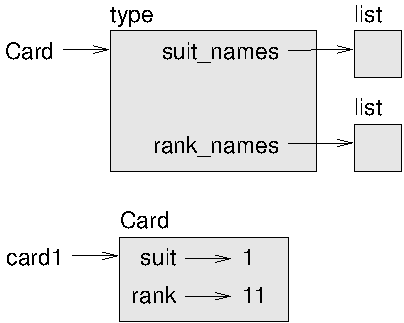
\includegraphics[scale=0.8]{figs/card1.pdf}}
 \caption{Διάγραμμα αντικειμένων.} 
\label{fig.card1}
\end{figure}

 Η Εικόνα~ \ref{fig.card1}  είναι ένα διάγραμμα του αντικειμένου της κλάσης  
{\tt Card}  και ένα του στιγμιότυπου  Card. 
\index{state diagram}
\index{diagram!state}
\index{object diagram}
\index{diagram!object}
Η  {\tt Card}  είναι μία κλάση αντικειμένων, άρα έχει τύπο   {\tt type}.  
Το  {\tt card1}  έχει τύπο  {\tt Card}.  (Για εξοικονόμηση χώρου, δεν 
σχεδίασα τα περιεχόμενα των  \verb"suit_names"  και  \verb"rank_names" ).



\section{Συγκρίνοντας τραπουλόχαρτα}
\label{comparecard}
\index{operator!relational}
\index{relational operator}

Για τους ενσωματωμένους τύπους υπάρχουν σχεσιακοί τελεστές  ({\tt <}, {\tt >}, {\tt ==},   κτλ. )  οι συγκρίνουν τιμές και προσδιορίζουν ποια είναι μεγαλύτερη, ποια είναι μικρότερη ή αν είναι ίσες.  Για τους τύπους που είναι ορισμένοι από το χρήστη, μπορούμε να παρακάμψουμε τη συμπεριφορά των ενσωματωμένων τελεστών παρέχοντας μία μέθοδο 
με όνομα  \verb"__cmp__".

 Η  \verb"__cmp__"  παίρνει δύο παραμέτρους, την  {\tt self}  και την   {\tt other},  και επιστρέφει ένα θετικό αριθμό αν το πρώτο αντικείμενο είναι 
μεγαλύτερο, ένα αρνητικό αριθμό αν το δεύτερο αντικείμενο είναι μεγαλύτερο και 0 αν είναι 
ίσα το ένα με το άλλο.
\index{override}
\index{operator overloading}

Η σωστή σειρά για τα τραπουλόχαρτα δεν είναι προφανής.  Ποιο είναι καλύτερο για παράδειγμα, το 3 σπαθί ή το 2 καρό ;   Το ένα έχει υψηλότερη τάξη αλλά το άλλο 
έχει μεγαλύτερο χρώμα.  Προκειμένου να μπορέσετε να συγκρίνετε τραπουλόχαρτα, πρέπει να 
αποφασίσετε ποιο από τα δύο, η τάξη ή το χρώμα, είναι σημαντικότερο.

Η απάντηση μπορεί να εξαρτάται από το παιχνίδι που παίζετε, αλλά για να απλοποιήσουμε  
τα πράγματα, θα κάνουμε την αυθαίρετη επιλογή ότι το χρώμα είναι σημαντικότερο, άρα όλα 
τα μπαστούνια είναι είναι ανώτερα από όλα τα καρό και ούτω καθεξής.
\index{cmp method@\_\_cmp\_\_ method}
\index{method!\_\_cmp\_\_}

Με βάση αυτό μπορούμε να γράψουμε την  \verb"__cmp__":

\begin{verbatim}
# inside class Card:

    def __cmp__(self, other):
        # check the suits
        if self.suit > other.suit: return 1
        if self.suit < other.suit: return -1

        # suits are the same... check ranks
        if self.rank > other.rank: return 1
        if self.rank < other.rank: return -1

        # ranks are the same... it's a tie
        return 0
\end{verbatim}
%
 Μπορείτε να την γράψετε πιο συνοπτικά χρησιμοποιώντας σύγκριση πλειάδων :
\index{tuple!comparison}
\index{comparison!tuple}

\begin{verbatim}
# inside class Card:

    def __cmp__(self, other):
        t1 = self.suit, self.rank
        t2 = other.suit, other.rank
        return cmp(t1, t2)
\end{verbatim}
%
 η ενσωματωμένη συνάρτηση  {\tt cmp}  έχει την ίδια διεπαφή με τη μέθοδο  
\verb"__cmp__":  παίρνει δύο τιμές και επιστρέφει ένα θετικό αριθμό αν η πρώτη είναι 
μεγαλύτερη, έναν αρνητικό αν η δεύτερη είναι μεγαλύτερη και 0 αν είναι ίσες.
\index{cmp function}
\index{function!cmp}

Στην  Python 3  δεν υπάρχει πλέον η  {\tt cmp}  και η μέθοδος  \verb"__cmp__"  δεν υποστηρίζεται.  Αντί αυτών θα πρέπει να παρέχετε την  \verb"__lt__",  η οποία επιστρέφει  {\tt True}  αν η  {\tt self}  είναι 
μικρότερη της  {\tt other}.   Μπορείτε να υλοποιήσετε την  \verb"__lt__"  χρησιμοποιώντας πλειάδες και τον τελεστή  \verb"<".


 
\begin{exercise}

Γράψτε μία μέθοδο  \verb"__cmp__"  για αντικείμενα  Time.   Σημείωση : 
 μπορείτε να χρησιμοποιήσετε σύγκριση πλειάδων, αλλά λάβετε υπόψιν σας ότι μπορείτε 
να χρησιμοποιήσετε και αφαίρεση ακεραίων.	

\end{exercise}
%    def __cmp__(self, other):
%        return time_to_int(self) - time_to_int(other)

%If {\tt self} is later than {\tt other}, the result is
%a positive number.  If {\tt other} is later, the result
%is negative.  And if {\tt self} and {\tt other} are equal
%(but not necessarily identical)
%the result is zero.



\section{Τράπουλες}
\index{list!of objects}
\index{deck, playing cards}

Τώρα που έχουμε τραπουλόχαρτα, το επόμενο βήμα είναι να ορίσουμε τράπουλες.  Αφού μία 
τράπουλα αποτελείται από τραπουλόχαρτα, είναι φυσικό κάθε τράπουλα να περιέχει μία λίστα 
από τραπουλόχαρτα σαν μία ιδιότητα.
\index{init method}
\index{method!init}

Το παρακάτω είναι ένας ορισμός κλάσης για τράπουλες.  Η μέθοδος  init  δημιουργεί 
την ιδιότητα  {\tt cards}  και παράγει ένα τυπικό σύνολο από πενήντα δύο φίλα :
\index{composition}
\index{loop!nested}
\index{Deck class}
\index{class!Deck}

\begin{verbatim}
class Deck(object):

    def __init__(self):
        self.cards = []
        for suit in range(4):
            for rank in range(1, 14):
                card = Card(suit, rank)
                self.cards.append(card)
\end{verbatim}
%
 Ο ευκολότερος τρόπος για να συμπληρώσουμε μία τράπουλα είναι με έναν εμφωλευμένο 
βρόχο.  Ο εξωτερικός βρόχος απαριθμεί τα χρώματα από το 0 έως το 3.  Ο εσωτερικός βρόχος 
απαριθμεί τις τάξεις από το 1 έως το 13.  Κάθε επανάληψη δημιουργεί ένα νέο τραπουλόχαρτο 
με το τρέχον χρώμα και τάξη, και το προσαρτά στην  {\tt self.cards}.
\index{append method}
\index{method!append}


 
\section{Τύπωση τράπουλας}
\label{printdeck}
\index{str method@\_\_str\_\_ method}
\index{method!\_\_str\_\_}

Αυτή είναι μία μέθοδος  \verb"__str__"  για την  {\tt Deck}:

\begin{verbatim}
#inside class Deck:

    def __str__(self):
        res = []
        for card in self.cards:
            res.append(str(card))
        return '\n'.join(res)
\end{verbatim}
%
 Αυτή η μέθοδος επιδεικνύει έναν αποδοτικό τρόπο για τη συσσώρευση μίας μεγάλης 
συμβολοσειράς :  φτιάχνοντας μία λίστα συμβολοσειρών και στη συνέχεια χρησιμοποιώντας την  {\tt join}.   Η ενσωματωμένη συνάρτηση  {\tt str}  επικαλείται τη μέθοδο  \verb"__str__"  σε κάθε φίλο και επιστρέφει μία αναπαράσταση 
συμβολοσειράς. 
\index{accumulator!string}
\index{string!accumulator}
\index{join method}
\index{method!join}
\index{newline}

Από τη στιγμή που επικαλεστήκαμε την  {\tt join}  σε έναν χαρακτήρα νέας γραμμής, τα 
φύλλα θα είναι χωρισμένα με νέες γραμμές.  Αυτό είναι το αποτέλεσμα : 

\begin{verbatim}
>>> deck = Deck()
>>> print deck
Ace of Clubs
2 of Clubs
3 of Clubs
...
10 of Spades
Jack of Spades
Queen of Spades
King of Spades
\end{verbatim}
%
 Παρόλο που το αποτέλεσμα εμφανίζεται σε 52 γραμμές, είναι μία μεγάλη συμβολοσειρά 
η οποία περιέχει νέες γραμμές.



\section{Προσθήκη, αφαίρεση, ανακάτεμα και ταξινόμηση}

Για να μοιράσουμε φύλλα, χρειαζόμαστε μία μέθοδο η οποία θα αφαιρεί ένα φύλλο από την 
τράπουλα και θα το επιστρέφει.  Η μέθοδος λιστών  {\tt pop}  παρέχει έναν εύκολο 
τρόπο για να γίνει αυτό :
\index{pop method}
\index{method!pop}

\begin{verbatim}
#inside class Deck:

    def pop_card(self):
        return self.cards.pop()
\end{verbatim}
%
 Αφού η  {\tt pop}  αφαιρεί το τελευταίο φύλλο της λίστας, σημαίνει ότι μοιράζουμε από το τέλος της τράπουλας.  Στην πραγματικότητα το μοίρασμα από το τέλος δεν είναι σωστό, αλλά στην προκειμένη περίπτωση δεν υπάρχει πρόβλημα.
\index{append method}
\index{method!append}

Για να προσθέσουμε ένα φύλλο, μπορούμε να χρησιμοποιήσουμε την μέθοδο λιστών  {\tt append}:

\begin{verbatim}
#inside class Deck:

    def add_card(self, card):
        self.cards.append(card)
\end{verbatim}
%
 Μία τέτοια μέθοδος η οποία χρησιμοποιεί μία άλλη συνάρτηση χωρίς να κάνει πολύ 
δουλειά από μόνη της ονομάζεται καπλαμάς  ({\bf veneer}).   Η έκφραση προέρχεται 
από την επεξεργασία του ξύλου, όπου συνηθίζεται να κολλάμε ένα λεπτό στρώμα καλής ποιότητας ξύλου στην επιφάνεια ενός φθηνότερου κομματιού ξύλου.
\index{veneer}

Στην συγκεκριμένη περίπτωση ορίζουμε μία  " λεπτή "  μέθοδο η οποία εκφράζει 
μία λειτουργία της λίστας με όρους που είναι κατάλληλοι για τράπουλες.

Σαν ένα ακόμα παράδειγμα, μπορούμε να γράψουμε μία μέθοδο με όνομα  {\tt shuffle}  
χρησιμοποιώντας τη συνάρτηση  {\tt shuffle}  του αρθρώματος  {\tt random}:
\index{random module}
\index{module!random}
\index{shuffle function}
\index{function!shuffle}

\begin{verbatim}
# inside class Deck:

    def shuffle(self):
        random.shuffle(self.cards)
\end{verbatim}
%
 Μην ξεχάσετε να εισάγετε το άρθρωμα  {\tt random}. 

\begin{exercise}
\index{sort method}
\index{method!sort}

Γράψτε μία μέθοδο για την  Deck  με όνομα  {\tt sort}  η οποία θα 
χρησιμοποιεί τη μέθοδο λιστών  {\tt sort}  για να ταξινομήσει τα φύλλα.  
Η  {\tt sort}  θα χρησιμοποιεί τη μέθοδο  \verb"__cmp__"  που ορίσαμε για να 
καθορίσουμε τη σειρά ταξινόμησης.

\end{exercise}


\section{Κληρονομικότητα}
\index{inheritance}
\index{object-oriented programming}

Το χαρακτηριστικό  της γλώσσας που την συνδέει περισσότερο με τον αντικειμενοστραφή 
προγραμματισμό η κληρονομικότητα.  Κληρονομικότητα είναι η δυνατότητα να ορίσουμε μία 
νέα κλάση η οποία θα είναι μία τροποποιημένη έκδοση μίας υπάρχουσας κλάσης.
\index{parent class}
\index{child class}
\index{class!child}
\index{subclass}
\index{superclass}

Ονομάζεται  " κληρονομικότητα "  επειδή η νέα κλάση κληρονομεί τις μεθόδους 
της υπάρχουσας κλάσης.  Επεκτείνοντας αυτήν τη μεταφορά, η υπάρχουσα κλάση ονομάζεται 
γονέας και η νέα κλάση ονομάζεται παιδί.

Σαν παράδειγμα, ας πούμε ότι θέλουμε μία κλάση για να αναπαραστήσουμε ένα 
 " χέρι ",  δηλαδή το σύνολο των καρτών που έχει στην κατοχή του ένας 
παίκτης.  Ένα χέρι είναι παρόμοιο με μία τράπουλα :  και τα δύο είναι φτιαγμένα 
από σύνολα φύλλων, και τα δύο χρειάζονται λειτουργίες όπως προσθήκης και αφαίρεσης φύλλων.

Ένα χέρι όμως είναι και διαφορετικό από μία τράπουλα :  υπάρχουν λειτουργίες που 
θέλουμε να έχουν τα χέρια αλλά δεν έχουν νόημα για μια τράπουλα.  Για παράδειγμα, στο 
πόκερ μπορεί να συγκρίνουμε δύο χέρια για να δούμε ποιο κερδίζει.  Στη γέφυρα, μπορεί να 
υπολογίσουμε ένα σκορ για ένα χέρι προκειμένου να κάνουμε ένα ποντάρισμα.

Αυτή η σχέση μεταξύ κλάσεων (όμοιες αλλά διαφορετικές) προσφέρεται για κληρονομικότητα.

Ο ορισμός μίας κλάσης παιδί είναι όπως οι ορισμοί των άλλων κλάσεων, με τη διαφορά ότι 
το όνομα της κλάσης γονέας εμφανίζεται μέσα σε παρενθέσεις :
\index{parentheses!parent class in}
\index{parent class}
\index{class!parent}
\index{Hand class}
\index{class!Hand}

\begin{verbatim}
class Hand(Deck):
    """Represents a hand of playing cards."""
\end{verbatim}
%
 Αυτός ο ορισμός υποδεικνύει ότι η  Hand  κληρονομεί την  {\tt Deck}.   
Αυτό σημαίνει ότι μπορούμε να χρησιμοποιήσουμε μεθόδους όπως η  \verb"pop_card"   και η  \verb"add_card"  τόσο για χέρια όσο και για τράπουλες.

Η  {\tt Hand}  κληρονομεί επίσης και την  \verb"__init__"  από την  {\tt Deck},  αλλά δεν κάνει αυτό που πραγματικά θα θέλαμε.  Αντί να γεμίζει το χέρι με 52 
νέα φύλλα, θα έπρεπε να αρχικοποιεί την  {\tt cards}  με μία κενή λίστα.
\index{override}
\index{init method}
\index{method!init}

Αν παράσχουμε μία μέθοδο  init  στην κλάση  {\tt Hand},  τότε θα υπερισχύσει 
αυτής στην κλάση  {\tt Deck}:

\begin{verbatim}
# inside class Hand:

    def __init__(self, label=''):
        self.cards = []
        self.label = label
\end{verbatim}
%
 Άρα όταν δημιουργείτε ένα χέρι, η  Python  επικαλείται αυτήν την μέθοδο  init:

\begin{verbatim}
>>> hand = Hand('new hand')
>>> print hand.cards
[]
>>> print hand.label
new hand
\end{verbatim}
%
 Αλλά οι άλλες μέθοδοι κληρονομούνται από την  {\tt Deck},  και έτσι μπορούμε 
να χρησιμοποιήσουμε την  \verb"pop_card"  και την  \verb"add_card"  για να μοιράσουμε ένα φύλλο :

\begin{verbatim}
>>> deck = Deck()
>>> card = deck.pop_card()
>>> hand.add_card(card)
>>> print hand
King of Spades
\end{verbatim}
%
 Το επόμενο λογικό βήμα είναι να ενθυλακώσουμε αυτόν τον κώδικα μέσα σε μία μέθοδο 
με όνομα  \verb"move_cards":
\index{encapsulation}

\begin{verbatim}
#inside class Deck:

    def move_cards(self, hand, num):
        for i in range(num):
            hand.add_card(self.pop_card())
\end{verbatim}
%
 Η  \verb"move_cards"  παίρνει δύο ορίσματα, ένα αντικείμενο  Hand  
και τον αριθμό φύλλων που θα μοιραστούν.  Τροποποιεί την  {\tt self}  και την 
 {\tt hand},  και επιστρέφει  {\tt None}.

 Σε μερικά παιχνίδια, τα φύλλα μεταφέρονται από ένα χέρι πίσω στην τράπουλα.  
Μπορείτε να χρησιμοποιήσετε την  \verb"move_cards"  για οποιαδήποτε από αυτές 
τις λειτουργίες :  η  {\tt self}  μπορεί να είναι είτε μία τράπουλα είτε 
ένα χέρι και η  {\tt hand},  ανεξαρτήτως ονόματος, μπορεί να είναι ακόμα και μια  τράπουλα.

\begin{exercise}

Γράψτε μία μέθοδο για την  Deck  με όνομα  \verb"deal_hands"  η οποία 
θα παίρνει δύο παραμέτρους, τον αριθμό των χεριών και τον αριθμό των φύλλων ανά χέρι.
Θα δημιουργεί αντικείμενα  Hand,  θα μοιράζει τον κατάλληλο αριθμό  φύλλων σε 
κάθε χέρι και θα επιστρέφει μία λίστα από αντικείμενα  Hand.

\end{exercise}

 Η κληρονομικότητα είναι ένα χρήσιμο χαρακτηριστικό.  Μερικά προγράμματα τα οποία 
θα ήταν επαναλαμβανόμενα χωρίς κληρονομικότητα μπορούν να γραφτούν πιο κομψά με αυτή.  
Η κληρονομικότητα μπορεί να διευκολύνει την επαναχρησιμοποίηση κώδικα, αφού μπορείτε 
να προσαρμόσετε την συμπεριφορά των γονικών κλάσεων χωρίς να χρειαστεί να τις τροποποιήσετε.  Σε μερικές περιπτώσεις, η δομή της κληρονομικότητας αντανακλά τη φυσική 
δομή του προβλήματος, το οποίο κάνει ευκολότερη την κατανόηση του προβλήματος.

Από την άλλη μεριά, η κληρονομικότητα μπορεί να κάνει δυσκολότερη την ανάγνωση 
των προγραμμάτων.  Μερικές φορές, όταν επικαλείται μία μέθοδος δεν είναι ξεκάθαρο 
που θα βρούμε τον ορισμό της.  Ο σχετικός κώδικας μπορεί να είναι διασκορπισμένος 
σε διάφορα αρθρώματα.  Επίσης, πολλά πράγματα που μπορούν να γίνουν χρησιμοποιώντας 
κληρονομικότητα μπορούν να γίνουν επίσης ή και καλύτερα χωρίς αυτήν.



\section{Διαγράμματα κλάσεων}
\label{class.diagram}

Μέχρι στιγμής έχουμε δει διαγράμματα στοίβας, τα οποία δείχνουν την κατάσταση 
ενός προγράμματος, και διαγράμματα αντικειμένων, τα οποία δείχνουν τις ιδιότητες 
ενός αντικειμένου και τις τιμές τους.  Αυτά τα διαγράμματα αναπαριστούν ένα στιγμιότυπο 
της εκτέλεσης ενός προγράμματος, επομένως αλλάζουν όσο τρέχει το πρόγραμμα.

Είναι επίσης πολύ λεπτομερή και σε ορισμένες περιπτώσεις πάρα πολύ λεπτομερή.  
Ένα διάγραμμα κλάσης είναι μία πιο αφηρημένη αναπαράσταση της δομής ενός προγράμματος.  
Αντί να δείχνει τα επιμέρους αντικείμενα, δείχνει τις κλάσεις και τις σχέσεις μεταξύ τους.

Υπάρχουν διάφορα είδη σχέσεων μεταξύ κλάσεων : 

\begin{itemize}

\item Τα αντικείμενα μίας κλάσης μπορεί να περιέχουν αναφορές σε αντικείμενα άλλων 
κλάσεων.  Για παράδειγμα, κάθε  Rectangle  περιέχει μία αναφορά σε ένα  Point, 
 και κάθε  Deck  περιέχει αναφορές σε πολλά  Cards.   Αυτού του είδους η σχέση ονομάζεται  " ΕΧΕΙ-ΕΝΑ ",  όπως στη φράση  " ένα  Rectangle     έχει ένα  Point". 

\item Μία κλάση μπορεί να κληρονομεί από μία άλλη.  Αυτή η σχέση ονομάζεται  " 
ΕΙΝΑΙ-ΕΝΑ ",  όπως στη φράση  " ένα  Hand  είναι ένα είδος μίας  Deck". 

\item Μία κλάση μπορεί να εξαρτάται από μία άλλη υπό την έννοια ότι οι αλλαγές σε 
μία κλάση θα απαιτούσαν αλλαγές και στην άλλη.

\end{itemize}
\index{IS-A relationship}
\index{HAS-A relationship}
\index{class diagram}
\index{diagram!class}

Ένα διάγραμμα κλάσεων είναι μία γραφική αναπαράσταση αυτών των σχέσεων.  Για παράδειγμα, 
η Εικόνα~ \ref{fig.class1}  δείχνει τις σχέσεις μεταξύ των  {\tt Card}, {\tt Deck}  και  {\tt Hand}.  


\begin{figure}
\centerline
{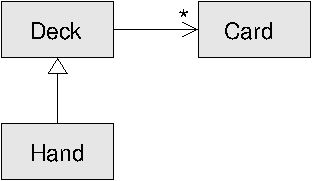
\includegraphics[scale=0.8]{figs/class1.pdf}}
\caption {Διάγραμμα κλάσεων.}
\label{fig.class1}
\end{figure}


Το βέλος με το κοίλο τριγωνάκι αναπαριστά μία σχέση ΕΙΝΑΙ-ΕΝΑ.  Σε αυτήν την 
περίπτωση υποδεικνύει ότι ένα  Hand  κληρονομεί από μία  Deck.

 Το κλασικό βέλος αναπαριστά μία σχέση ΕΧΕΙ-ΕΝΑ. Σε αυτήν την περίπτωση μία  
Deck  έχει αναφορές σε αντικείμενα  Card.
\index{multiplicity (in class diagram)}

 Το αστεράκι  ({\tt *})  δίπλα στο βέλος είναι μία πολλαπλότητα, η οποία 
δείχνει πόσα φύλλα έχει μία τράπουλα.  Μία πολλαπλότητα μπορεί να είναι ένας απλός 
αριθμός, όπως το  {\tt 52},  ένα εύρος, όπως το  {\tt 5..7},  ή ένα αστεράκι 
το οποίο υποδεικνύει ότι μία τράπουλα μπορεί να έχει έναν οποιοδήποτε αριθμό φύλλων.

Ένα πιο λεπτομερές διάγραμμα μπορεί να δείχνει ότι μία τράπουλα περιέχει μία λίστα 
από φύλλα, αλλά οι ενσωματωμένοι τύποι όπως οι λίστες και τα λεξικά δεν περιλαμβάνονται 
σε διαγράμματα κλάσεων.


\begin{exercise}

Διαβάστε τα  {\tt TurtleWorld.py}, {\tt World.py}  και  {\tt Gui.py}  και 
σχεδιάστε ένα διάγραμμα κλάσεων το οποίο θα δείχνει τις σχέσεις μεταξύ των κλάσεων που 
ορίζονται εκεί.

\end{exercise}


\section{Αποσφαλμάτωση}
\index{debugging}

Η κληρονομικότητα μπορεί να κάνει την αποσφαλμάτωση μία πρόκληση επειδή όταν 
επικαλείστε μία μέθοδο σε ένα αντικείμενο, μπορεί να μην ξέρετε ποια μέθοδος 
επικαλείται.
\index{polymorphism}

Υποθέστε ότι γράφετε μία συνάρτηση η οποία θα δουλεύει με αντικείμενα  Hand.  
 Τότε, σίγουρα, Θα θέλατε να δουλεύει με όλα τα είδη χεριών, όπως τα  PokerHands, BridgeHands  και ούτω καθεξής.  Αν επικαλεστείτε μία μέθοδο όπως τη  {\tt shuffle}, 
 μπορεί να πάρετε αυτήν που ορίστηκε στην  {\tt Deck},  αλλά αν κάποια από 
τις υποκλάσεις παρακάμψει αυτήν τη μέθοδο τότε θα πάρετε εκείνη την έκδοση.
\index{flow of execution}

Κάθε φορά που δεν είστε σίγουροι για την ροή εκτέλεσης του προγράμματός σας, η 
απλούστερη λύση είναι να προσθέσετε δηλώσεις  print  στην αρχή των σχετικών 
μεθόδων.  Αν η  {\tt Deck.shuffle}  εμφανίσει ένα μήνυμα το οποίο λέει κάτι 
τέτοιο  {\tt Running Deck.shuffle},  τότε ιχνηλατεί τη ροή εκτέλεσης καθώς 
τρέχει το πρόγραμμα.

Μία εναλλακτική λύση είναι να χρησιμοποιήσετε αυτήν την συνάρτηση, η οποία παίρνει 
ένα αντικείμενο και ένα όνομα μεθόδου (σαν συμβολοσειρά) και επιστρέφει την κλάση η 
οποία παρέχει τον ορισμό της μεθόδου :

\begin{verbatim}
def find_defining_class(obj, meth_name):
    for ty in type(obj).mro():
        if meth_name in ty.__dict__:
            return ty
\end{verbatim}
%
 Αυτό είναι ένα παράδειγμα :

\begin{verbatim}
>>> hand = Hand()
>>> print find_defining_class(hand, 'shuffle')
<class 'Card.Deck'>
\end{verbatim}
%
 Άρα η μέθοδος  {\tt shuffle}  για αυτό το χέρι είναι αυτή στην  {\tt Deck}.
\index{mro method}
\index{method!mro}
\index{method resolution order}

 Η  \verb"find_defining_class"  χρησιμοποιεί τη μέθοδο  {\tt mro}  για να 
για να πάρει τη λίστα των αντικειμένων των κλάσεων που θα αναζητηθούν για για μεθόδους.  
 ``MRO''  είναι τα αρχικά από  ``method resolution order.''
\index{override}
\index{interface}
\index{precondition}
\index{postcondition}

 Αυτή είναι μία πρόταση σχεδιασμού ενός προγράμματος :  όποτε παρακάμπτετε μία 
μέθοδο, η διεπαφή την νέας μεθόδου θα πρέπει να είναι ίδια με της παλιάς.  Θα πρέπει να 
παίρνει τις ίδιες παραμέτρους, να επιστρέφει τον ίδιο τύπο, και να υπακούει στις ίδιες 
προϋποθέσεις και μετασυνθήκες.  Αν ακολουθήσετε αυτόν τον κανόνα, θα ανακαλύψετε ότι κάθε 
συνάρτηση η οποία σχεδιάστηκε για να δουλεύει με ένα στιγμιότυπο μία υπερκλάσης, όπως η 
 Deck,  δουλεύει επίσης και με στιγμιότυπα των υποκλάσεων όπως της  Hand  ή της  PokerHand.

 Αν παραβιάσετε αυτόν τον κανόνα, ο κώδικάς σας θα καταρρεύσει σαν ένα σπίτι από 
τραπουλόχαρτα.



\section{Ενθυλάκωση δεδομένων}

Το Κεφάλαιο~ \ref{time}  επιδεικνύει ένα πλάνο ανάπτυξης που θα μπορούσαμε 
να αποκαλέσουμε  " αντικειμενοστραφή σχεδίαση ".   Προσδιορίσαμε τα αντικείμενα 
που χρειαζόμασταν  ({\tt Time}, {\tt Point}  και  {\tt Rectangle})  και ορίσαμε 
κλάσεις για να τα αναπαραστήσουμε.  Για κάθε περίπτωση υπάρχει μία προφανής αντιστοίχιση 
μεταξύ ενός αντικειμένου με κάποια οντότητα του πραγματικού κόσμου (ή τουλάχιστον ενός μαθηματικού κόσμου).
\index{development plan}

Αλλά μερικές φορές δεν είναι προφανές τι αντικείμενα χρειάζεστε και πως θα πρέπει να 
αλληλεπιδρούν.  Σε αυτήν την περίπτωση χρειάζεστε ένα διαφορετικό πλάνο ανάπτυξης.  Με 
τον ίδιο τρόπο που ανακαλύψαμε τις διεπαφές των συναρτήσεων ενθυλακώνοντας και 
γενικεύοντας, μπορούμε να ανακαλύψουμε και τις διεπαφές των κλάσεων ενθυλακώνοντας δεδομένα.
\index{data encapsulation}
\index{encapsulation!data}

Η ανάλυση Μαρκόφ, από την Ενότητα~ \ref{markov},  παρέχει ένα καλό παράδειγμα.  
Αν κατεβάσετε τον κώδικά μου από τον σύνδεσμο  \url{http://thinkpython.com/code/markov.py},  θα δείτε ότι χρησιμοποιεί δύο καθολικές 
μεταβλητές, την  \verb"suffix_map"  και την  \verb"prefix",  οι οποίες διαβάζονται και γράφονται από αρκετές συναρτήσεις. 

\begin{verbatim}
suffix_map = {}
prefix = ()
\end{verbatim}

 Επειδή αυτές οι μεταβλητές είναι καθολικές μπορούμε να τρέξουμε μία ανάλυση τη φορά. 
Αν διαβάσουμε δύο κείμενα, τα προθέματα και τα επιθέματα τους θα προστεθούν στις ίδιες 
δομές δεδομένων (το οποίο δημιουργεί κάποιο ενδιαφέρον κείμενο).

Για να τρέξουμε πολλαπλές αναλύσεις, και να τις κρατήσουμε χωριστά, μπορούμε να ενθυλακώσουμε την κατάσταση κάθε ανάλυσης σε ένα αντικείμενο. Κάπως έτσι δηλαδή :

\begin{verbatim}
class Markov(object):

    def __init__(self):
        self.suffix_map = {}
        self.prefix = ()
\end{verbatim}

 Στη συνέχεια, μετατρέπουμε τις συναρτήσεις σε μεθόδους. Για παράδειγμα, αυτή 
είναι η  \verb"process_word":

\begin{verbatim}
    def process_word(self, word, order=2):
        if len(self.prefix) < order:
            self.prefix += (word,)
            return

        try:
            self.suffix_map[self.prefix].append(word)
        except KeyError:
            # if there is no entry for this prefix, make one
            self.suffix_map[self.prefix] = [word]

        self.prefix = shift(self.prefix, word)
\end{verbatim}

 Η μετατροπή ενός προγράμματος κατά αυτό τον τρόπο, αλλάζοντας τον σχεδιασμό χωρίς να αλλάξουμε τη συνάρτηση, είναι ένα ακόμα παράδειγμα ανακατασκευής κώδικα (βλ. Ενότητα~ \ref{refactoring}).
\index{refactoring}

 Αυτό το παράδειγμα προτείνει ένα πλάνο ανάπτυξης για το σχεδιασμό αντικειμένων και μεθόδων :

\begin{enumerate}

 
\item Ξεκινήστε γράφοντας συναρτήσεις οι οποίες θα διαβάζουν και θα γράφουν καθολικές 
μεταβλητές (όταν είναι απαραίτητο).

\item Αφού φτιάξετε ένα λειτουργικό πρόγραμμα, ψάξτε για συσχετίσεις μεταξύ των καθολικών 
μεταβλητών και των συναρτήσεων που τις χρησιμοποιούν.

\item Ενθυλακώστε σχετικές μεταβλητές ως ιδιότητες ενός αντικειμένου.

\item Μετατρέψτε τις αντίστοιχες συναρτήσεις σε μεθόδους μίας νέας κλάσης.
 

\end{enumerate}


\begin{exercise}

Κατεβάστε τον κώδικά μου από την Ενότητα~ \ref{markov} (\url{http://thinkpython.com/code/markov.py}),  και ακολουθήστε τα βήματα που 
περιγράψαμε παραπάνω για να ενθυλακώσετε τις καθολικές μεταβλητές σαν ιδιότητες μίας νέας 
κλάσης με όνομα  {\tt Markov}.  Λύση : \url{http://thinkpython.com/code/Markov.py} (προσοχή στο κεφαλαίο Μ).

\end{exercise}




\section{Ορολογία}

\begin{description}

\item[κωδικοποίηση:]  Η αναπαράσταση ενός συνόλου τιμών χρησιμοποιώντας ένα άλλο 
σύνολο τιμών και υλοποιώντας μία αντιστοίχιση μεταξύ τους.
\index{encode}

\item[ιδιότητα κλάσης:] Μία ιδιότητα που σχετίζεται με ένα αντικείμενο κλάσης.  Οι 
ιδιότητες των κλάσεων ορίζονται μέσα στον ορισμό μιας κλάσης αλλά έξω από οποιαδήποτε 
μέθοδο.
\index{class attribute}
\index{attribute!class}

\item[ιδιότητα στιγμιότυπου:] Μία ιδιότητα που σχετίζεται με ένα στιγμιότυπο μιας κλάσης.
\index{instance attribute}
\index{attribute!instance}

\item[καπλαμάς:] Μία μέθοδος ή μία συνάρτηση η οποία παρέχει μία διαφορετική 
διεπαφή σε μία άλλη συνάρτηση χωρίς να κάνει κάποιον ιδιαίτερο υπολογισμό.
\index{veneer}

\item[κληρονομικότητα:] Η ικανότητα να ορίσουμε μία νέα κλάση η οποία είναι 
μία τροποποιημένη έκδοση μίας ήδη ορισμένης κλάσης.
\index{inheritance}

\item[κλάση γονέας:] Η κλάση από όπου μία κλάση παιδί κληρονομεί.
\index{parent class}

\item[κλάση παιδί:] Μία νέα κλάση που δημιουργήθηκε κληρονομώντας μία υπάρχουσα κλάση. 
Ονομάζεται επίσης και  " υποκλάση ". 
\index{child class}
\index{class!child}

\item[σχέση ΕΙΝΑΙ-ΕΝΑ:] Η σχέση μεταξύ μίας κλάσης παιδί και της κλάσης γονέα.
\index{IS-A relationship}

\item[σχέση ΕΧΕΙ-ΕΝΑ:] Η σχέση μεταξύ δύο κλάσεων όπου τα στιγμιότυπα της μίας κλάσης 
περιέχουν αναφορές στα στιγμιότυπα της άλλης.
\index{HAS-A relationship}

\item[διάγραμμα κλάσεων:] Ένα διάγραμμα το οποίο δείχνει τις κλάσεις ενός προγράμματος 
και τις σχέσεις μεταξύ τους.
\index{class diagram}
\index{diagram!class}

\item[πολλαπλότητα:] Μία σημειογραφία σε ένα διάγραμμα κλάσεων η οποία δείχνει, για μία 
σχέση ΕΧΕΙ-ΕΝΑ, πόσες αναφορές υπάρχουν σε στιγμιότυπα μίας άλλης κλάσης.
\index{multiplicity (in class diagram)}

\end{description}



\section{Ασκήσεις}

\begin{exercise}
\label{poker}

Τα ακόλουθα είναι τα πιθανά χέρια στο πόκερ, σε αύξουσα σειρά αξίας (και φθίνουσα 
σειρά πιθανότητας) :
\index{poker}

\begin{description}

\item[pair:]  δύο φύλλα της ίδιας τάξης 
\vspace{-0.05in}

\item[two pair:]  δύο ζεύγη φύλλων 
\vspace{-0.05in}

\item[three of a kind:]  τρία φύλλα της ίδιας τάξης 
\vspace{-0.05in}

\item[straight:]  πέντε φύλλα στη σειρά (οι άσοι μπορούν να είναι είτε υψηλής είτε χαμηλής τάξης, έτσι το Άσος-2-3-4-5 και το 10-Βαλές-Ντάμα-Παπάς-Άσος είναι κέντα αλλά το Ντάμα-Παπάς-Άσος-2-3 δεν είναι). 
\vspace{-0.05in}

\item[flush:]  πέντε φύλλα με το ίδιο χρώμα 
\vspace{-0.05in}

\item[full house:]  τρία φύλλα ίδιας τάξης και ένα ζεύγος 
\vspace{-0.05in}

\item[four of a kind:]  τέσσερα φύλλα της ίδιας τάξης 
\vspace{-0.05in}

\item[straight flush:]  πέντε φύλλα στη σειρά με το ίδιο χρώμα 
\vspace{-0.05in}

\end{description}
%
 Στόχος αυτών των ασκήσεων είναι ο υπολογισμός της πιθανότητας να σχεδιαστούν 
αυτά τα χέρια.

\begin{enumerate}

\item Κατεβάστε αυτά τα αρχεία από το σύνδεσμο  \url{http://thinkpython.com/code}:

\begin{description}

\item[{\tt Card.py}]:  Μία πλήρης έκδοση των κλάσεων  {\tt Card}, {\tt Deck}  
και  {\tt Hand}  αυτού του κεφαλαίου. 

\item[{\tt PokerHand.py}]:  Μία ελλιπή υλοποίηση μίας κλάσης που αναπαριστά ένα χέρι 
στο πόκερ και κάποιος κώδικας που την ελέγχει. 

\end{description}
%
 
\item Αν τρέξετε το  {\tt PokerHand.py},  θα δείτε ότι μοιράζει εφτά χέρια πόκερ των 
εφτά φύλλων και ελέγχει αν κάποιο από αυτά περιέχει  flush.   Διαβάστε προσεκτικά αυτόν τον κώδικα προτού συνεχίσετε.

\item Προσθέστε μεθόδους στο  {\tt PokerHand.py}  με ονόματα  \verb"has_pair", 
\verb"has_twopair"  κτλ. οι οποίες θα επιστρέφουν  True  ή  False  ανάλογα 
με το αν το χέρι ικανοποιεί ή όχι τα κατάλληλα κριτήρια.  Ο κώδικάς σας θα πρέπει να δουλεύει σωστά για όλα τα χέρια, ανεξαρτήτως του αριθμού των φύλλων που περιέχουν (παρόλο που τα συνηθέστερα μεγέθη είναι 5 και 7).

\item Γράψτε μία μέθοδο με όνομα  {\tt classify}  η οποία θα υπολογίζει την 
υψηλότερη αξία βάση του συνδυασμού των φύλλων για ένα χέρι και θα θέτει την ιδιότητα  {\tt label}  αναλόγως.  Για παράδειγμα, αν ένα χέρι 7 φύλλων περιέχει και ένα 
φλος και ένα ζεύγος, θα πρέπει να χαρακτηριστεί σαν φλος.

\item Όταν σιγουρευτείτε ότι οι μέθοδοι κατηγοριοποίησης δουλεύουν, τότε το επόμενο βήμα 
είναι να υπολογίσετε τις πιθανότητες των διαφόρων χεριών.  Γράψτε μία συνάρτηση μέσα στο 
 {\tt PokerHand.py}  η οποία θα ανακατεύει μία τράπουλα, θα την χωρίζει σε χέρια, 
θα κατηγοριοποιεί τα χέρια και θα μετράει πόσες φορές εμφανίζεται κάθε κατηγοριοποίηση.

\item Τυπώστε ένα πίνακα με τις κατηγοριοποιήσεις και τις πιθανότητές τους.  Τρέξτε το 
πρόγραμμα με όλο και μεγαλύτερο αριθμό χεριών μέχρι οι τιμές εξόδου να συγκλίνουν σε έναν 
ικανοποιητικό βαθμό ακρίβειας.  Συγκρίνετε τα αποτελέσματά σας με τις τιμές στην διεύθυνση 
 \url{http://en.wikipedia.org/wiki/Hand_rankings}. 

\end{enumerate}

Λύση : \url{http://thinkpython.com/code/PokerHandSoln.py}. 

\end{exercise}



\begin{exercise}
\index{Swampy}
\index{TurtleWorld}

Αυτή η άσκηση χρησιμοποιεί το  TurtleWorld  του Κεφαλαίου~ \ref{turtlechap}.   
Θα γράψετε κώδικα ο οποίος θα κάνει τις χελώνες να παίξουν  tag.  Αν δεν γνωρίζετε το 
παιχνίδι διαβάστε εδώ τους κανόνες : \url{http://en.wikipedia.org/wiki/Tag_(game)}.  

\begin{enumerate}

\item Κατεβάστε το  \url{http://thinkpython.com/code/Wobbler.py}  και τρέξτε το.  
Θα πρέπει να δείτε έναν  TurtleWorld  με τρεις χελώνες.   Αν πιέσετε το κουμπί 
 {\sf Run}  οι χελώνες περιπλανιούνται τυχαία.

\item Διαβάστε τον κώδικα και σιγουρευτείτε ότι καταλαβαίνετε πως δουλεύει.  
Η κλάση  {\tt Wobbler}  κληρονομεί την  {\tt Turtle},  που σημαίνει ότι 
οι μέθοδοι της  {\tt Turtle} {\tt lt}, {\tt rt}, {\tt fd}  και  {\tt bk}  
δουλεύουν και σε στιγμιότυπα  {\tt Wobbler}.  

Η μέθοδος  {\tt step}  επικαλείται από την  TurtleWorld.   Και αυτή με τη σειρά της επικαλείται την  
{\tt steer},  η οποία γυρίζει τη χελώνα στην επιθυμητή κατεύθυνση, την  {\tt wobble}, 
 η οποία κάνει μία τυχαία στροφή ανάλογα με την απροσεξία της χελώνας, 
και την  {\tt move},  η οποία τη μετακινεί μπροστά μερικά πίξελς ανάλογα με την ταχύτητα της.
\index{Tagger}

\item Δημιουργήστε ένα αρχείο με όνομα  {\tt Tagger.py}.   Εισάγετε τα πάντα 
  από την  {\tt Wobbler}  και στη συνέχεια ορίστε μία κλάση με όνομα  {\tt Tagger} 
   η οποία θα κληρονομεί την  {\tt Wobbler}.   Καλέστε την  \verb"make_world" 
   περνώντας την  {\tt Tagger}  σαν όρισμα.

\item Προσθέστε μία μέθοδο  {\tt steer}  στην  {\tt Tagger}  για να παρακάμψει 
  αυτή της  {\tt Wobbler}.   Αρχικά, γράψτε μία έκδοση η οποία στρέφει τη χελώνα στην 
  αρχική της κατεύθυνση.  Σημείωση :  χρησιμοποιήστε την μαθηματική συνάρτηση  
  {\tt atan2}  και τις ιδιότητες της χελώνας  {\tt x}, {\tt y}  και  
  {\tt heading}. 

\item Τροποποιήστε την  {\tt steer}  έτσι ώστε οι χελώνες να μένουν στα όρια. 
  Μπορείτε να χρησιμοποιήσετε το κουμπί  {\sf Step}  για την αποσφαλμάτωση, το 
  οποίο επικαλείται την  {\tt step}  μία φορά σε κάθε χελώνα.

\item Τροποποιήστε την  {\tt steer}  έτσι ώστε κάθε χελώνα να στρέφεται προς την 
  κοντινότερη γειτονική.  Σημείωση :  οι χελώνες έχουν μία ιδιότητα, την  
  {\tt world},  η οποία είναι μία αναφορά στον  TurtleWorld  που ζουν, και ο 
   TurtleWorld  έχει μία ιδιότητα, την  {\tt animals},  η οποία είναι μία λίστα 
  με όλες τις χελώνες του κόσμου.

\item Τροποποιήστε την  {\tt steer}  έτσι ώστε οι χελώνες να παίζουν  tag.   
  Μπορείτε να προσθέσετε μεθόδους στην  {\tt Tagger}  και να παρακάμψετε την  
  {\tt steer}  και την  \verb"__init__",  αλλά δεν μπορείτε να τροποποιήσετε ή 
  να παρακάμψετε την  {\tt step}, {\tt wobble}  ή  {\tt move}.   Επίσης, η  
  {\tt steer}  επιτρέπεται να αλλάζει την κατεύθυνση της χελώνας αλλά όχι την θέση της.

Προσαρμόστε τους κανόνες και την μέθοδο  {\tt steer}  για ένα παιχνίδι καλής 
ποιότητας.  Για παράδειγμα, θα πρέπει να είναι εφικτό για μία αργή χελώνα να κάνει  tag 
 τις γρηγορότερες.

\end{enumerate}

Λύση : \url{http://thinkpython.com/code/Tagger.py}.

\end{exercise}



\chapter{Tkinter}
\label{tkinter}

 
\section{Γραφική διασύνδεση χρήστη}

Τα περισσότερα από τα προγράμματα που έχουμε δει μέχρι στιγμής είναι βασισμένα σε κείμενο, 
αλλά πολλά προγράμματα χρησιμοποιούν γραφική διασύνδεση χρήστη, γνωστή και ως  {\bf GUI}.
\index{GUI}
\index{graphical user interface}
\index{Tkinter}

 Η  Python  παρέχει αρκετές επιλογές για την συγγραφή προγραμμάτων βασισμένα σε 
 GUI,  συμπεριλαμβανομένων των  wxPython, Tkinter,  και  Qt.   Καθένα 
έχει τα θετικά του και τα αρνητικά του, για αυτόν το λόγο η  Python  δεν συγκλίνει προς ένα πρότυπο.

Αυτό που θα σας παρουσιάσω σε αυτό το κεφάλαιο είναι το  Tkinter  επειδή πιστεύω 
ότι είναι το ευκολότερο με το οποίο μπορεί να αρχίσει κανείς.  Τα περισσότερα τα παραδείγματα αυτού του κεφαλαίου μπορούν να υλοποιηθούν και με τα άλλα αρθώματα.

Υπάρχουν αρκετά βιβλία και ιστοσελίδες σχετικά με το  Tkinter.  Μία από τις 
καλύτερες διαδικτυακές πηγές είναι το  {\em An Introduction to Tkinter}  του  
Fredrik Lundh.
\index{Gui module}
\index{module!Gui}
\index{Swampy}

 Έχω γράψει ένα άρθρωμα με όνομα  {\tt Gui.py}  το οποίο συνοδεύει το  
Swampy.   Παρέχει μία απλοποιημένη διασύνδεση με τις συναρτήσεις και τις κλάσεις του 
 Tkinter.   Τα παραδείγματα αυτού του κεφαλαίου είναι βασισμένα σε αυτό το άρθρωμα.

Αυτό είναι ένα απλό παράδειγμα το οποίο δημιουργεί και εμφανίζει μία γραφική διασύνδεση :

 Για να δημιουργήσετε μία τέτοια διασύνδεση, πρέπει να εισάγετε το  {\tt Gui}  από 
το  Swampy:
%
\begin{verbatim}
from swampy.Gui import *
\end{verbatim}
%
 Ή έτσι, ανάλογα με το πως εγκαταστήσατε το  Swampy:
%
\begin{verbatim}
from Gui import *
\end{verbatim}
%
 Στη συνέχεια δημιουργήστε ένα αντικείμενο  Gui:
%
\begin{verbatim}
g = Gui()
g.title('Gui')
g.mainloop()
\end{verbatim}
%
 Όταν τρέξετε αυτόν τον κώδικα, θα πρέπει να εμφανιστεί ένα παράθυρο με ένα κενό γκρι 
τετράγωνο και τον τίτλο  {\sf Gui}.   Η  {\tt mainloop}  τρέχει την  
{\bf event loop},  η οποία περιμένει το χρήστη να κάνει κάτι και αποκρίνεται ανάλογα.  
Είναι ένας ατέρμων βρόχος, ο οποίος τρέχει μέχρι ο χρήστης να κλείσει το παράθυρο ή να 
πατήσει  Control-C  ή να κάνει κάτι που θα προκαλέσει το κλείσιμο του προγράμματος.
\index{event loop}
\index{loop!event}
\index{infinite loop}
\index{loop!infinite}

Αυτό το  Gui  δεν κάνει πολλά επειδή δεν έχει καθόλου  {\bf widgets}.   
Τα  widgets  είναι στοιχεία τα οποία συνθέτουν ένα  GUI.   Περιλαμβάνουν :
\index{widget}

 
\begin{description}

\item[Κουμπί:] Ένα γραφικό στοιχείο, που περιέχει κείμενο ή εικόνα, το οποίο 
εκτελεί μία ενέργεια όταν πατηθεί.

\item[Καμβάς:] Μία περιοχή η οποία μπορεί να εμφανίσει γραμμές, ορθογώνια παραλληλόγραμμα, 
κύκλους και άλλα σχήματα.

\item[Είσοδος:] Μία περιοχή όπου οι χρήστες μπορούν να πληκτρολογήσουν κείμενο.

\item[Μπάρα κύλισης:] Ένα γραφικό στοιχείο το οποίο ρυθμίζει το ορατό μέρος ενός άλλου 
γραφικού στοιχείου.

\item[Πλαίσιο:] Ένας περιέκτης, συχνά αόρατος, ο οποίος περιέχει άλλα γραφικά στοιχεία.

\end{description}

Το κενό γκρι τετράγωνο που βλέπετε όταν δημιουργείτε ένα  Gui  είναι ένα πλαίσιο.  
Όταν δημιουργείτε ένα νέο γραφικό στοιχείο, τότε προστίθεται σε αυτό το πλαίσιο.



\section{Κουμπιά και επιστροφές κλήσεων}
\index{Button widget}
\index{widget!Button}

Η μέθοδος  {\tt bu}  δημιουργεί ένα κουμπί :

\begin{verbatim}
button = g.bu(text='Press me.')
\end{verbatim}
%
 Οι επιστρεφόμενη τιμή της  {\tt bu}  είναι ένα αντικείμενο  Button.   
Το κουμπί που εμφανίζεται στο πλαίσιο  (Frame)  είναι μία γραφική αναπαράσταση 
αυτού του αντικειμένου.  Μπορείτε να ρυθμίσετε το κουμπί επικαλλώντας μεθόδους πάνω του.
\index{option}

Η  {\tt bu}  παίρνει μέχρι 32 παραμέτρους οι οποίες την εμφάνιση και τη λειτουργία 
του κουμπιού.  Αυτές οι παράμετροι ονομάζονται {\bf επιλογές}.  Αντί να παρέχετε 
τιμές τιμές και για τις 32 επιλογές, μπορείτε να χρησιμοποιήσετε ορίσματα με λέξεις 
κλειδιά, όπως το  \verb"text='Press me.'",  για να ορίσετε μόνο τις επιλογές που 
χρειάζεστε και να χρησιμοποιήσετε τις προκαθορισμένες τιμές για τις υπόλοιπες.
\index{keyword argument}
\index{argument!keyword}

Όταν προσθέτετε ένα γραφικό στοιχείο στο πλαίσιο, τότε αυτό συρρικνώνεται γύρω από αυτό.  
Δηλαδή, το πλαίσιο συρρικνώνεται στο μέγεθος του κουμπιού.  Αν προσθέσετε περισσότερα 
γραφικά στοιχεία, το πλαίσιο μεγαλώνει για να τα φιλοξενήσει όλα.
\index{Label widget}
\index{widget!Label}

Η μέθοδος  {\tt la}  δημιουργεί μία επιγραφή (Label):

\begin{verbatim}
label = g.la(text='Press the button.')
\end{verbatim}
%
 Από προεπιλογή, το  Tkinter  στοιβάζει τα στοιχεία από πάνω προς τα κάτω και 
τα κεντράρει.  Θα δούμε πως παρακάμπτουμε αυτή τη συμπεριφορά σύντομα.

Αν πατήσετε το κουμπί, θα δείτε ότι δεν κάνει πολλά πράγματα.  
Αυτό συμβαίνει επειδή δεν το έχετε  " συνδέσει ",  δηλαδή δεν του έχετε πει 
τι να κάνει !

 Η επιλογή που ρυθμίζει τη συμπεριφορά ενός κουμπιού είναι η  {\tt command}.   
Η τιμή της  {\tt command}  είναι μία συνάρτηση η οποία εκτελείται όταν πατιέται το κουμπί.  Για παράδειγμα, αυτή η συνάρτηση δημιουργεί ένα νέο  Label:

\begin{verbatim}
def make_label():
    g.la(text='Thank you.')
\end{verbatim}
%
 Τώρα μπορούμε να δημιουργήσουμε ένα κουμπί με αυτήν την συνάρτηση ως εντολή  
(command):

\begin{verbatim}
button2 = g.bu(text='No, press me!', command=make_label)
\end{verbatim}
%
 Όταν πιέσετε αυτό το κουμπί, θα πρέπει να εκτελεστεί η  \verb"make_label"  
και να εμφανιστεί μία νέα επιγραφή.
\index{callback}

Η τιμή της επιλογής  {\tt command}  είναι ένα αντικείμενο συνάρτησης, το οποίο 
είναι γνωστό ως επιστροφή κλήσης  (callback),  επειδή αφού καλέσετε την  {\tt bu}  για να δημιουργήσετε ένα κουμπί, η ροή εκτέλεσης επιστρέφει την κλήση όταν ο χρήστης 
πατάει το κουμπί.
\index{event-driven programming}

Αυτού του είδους η ροή είναι χαρακτηριστικό του προγραμματισμού {\bf χειρισμού συμβάντων}.  
Οι ενέργειες του χρήστη, όπως το πάτημα ενός κουμπιού και οι πληκτρολογήσεις, ονομάζονται 
{\bf συμβάντα}.  Στον προγραμματισμό χειρισμού συμβάντων, η ροή εκτέλεσης καθορίζεται από 
τις ενέργειες του χρήστη αντί από τον προγραμματιστή.

Η πρόκληση με αυτόν τον προγραμματισμό είναι να κατασκευάσετε ένα σύνολο από γραφικά 
στοιχεία και επιστροφές κλήσεων τα οποία θα δουλεύουν σωστά (ή τουλάχιστον θα παράγουν 
τα κατάλληλα μηνύματα λάθους) για οποιαδήποτε σειρά ενεργειών του χρήστη.


\begin{exercise}

Γράψτε ένα πρόγραμμα το οποίο θα δημιουργεί μία διασύνδεση χρήστη με ένα κουμπί.  
Όταν πατηθεί αυτό το κουμπί θα πρέπει να δημιουργεί ένα δεύτερο κουμπί.  Και όταν 
πατηθεί το δεύτερο, θα πρέπει να δημιουργεί μία επιγραφή η οποία θα λέει : ``Nice job!''.

 Τι συμβαίνει αν πατήσετε τα κουμπιά παραπάνω από μία φορές ; 
Λύση : \url{http://thinkpython.com/code/button_demo.py}
\end{exercise}


 
\section{Γραφικά στοιχεία Καμβά}
\index{Canvas widget}
\index{widget!Canvas}

Ένα από τα πιο πολύπλευρα γραφικά στοιχεία είναι ο καμβάς, ο οποίος δημιουργεί 
μία περιοχή για τον σχεδιασμό γραμμών, κύκλων και άλλων σχημάτων.  Αν έχετε κάνει την 
Άσκηση~ \ref{canvas}  θα είστε ήδη εξοικειωμένοι με τους καμβάδες.

Η μέθοδος  {\tt ca}  δημιουργεί ένα νέο καμβά :

\begin{verbatim}
canvas = g.ca(width=500, height=500)
\end{verbatim}
%
 Η  {\tt width}  και η  {\tt height}  είναι οι διαστάσεις του καμβά σε 
εικονοστοιχεία.
\index{config method}
\index{method!config}

Μπορείτε να αλλάξετε τις τιμές των επιλογών, ακόμα και μετά την δημιουργία ενός γραφικού στοιχείου, με τη μέθοδο  {\tt config}.   Για παράδειγμα, η επιλογή  {\tt bg}  
αλλάζει το χρώμα του φόντου :

\begin{verbatim}
canvas.config(bg='white')
\end{verbatim}
%
 Η τιμή της  {\tt bg}  είναι μία συμβολοσειρά με το όνομα ενός χρώματος.  
Το σύνολο των έγκυρων ονομάτων για τα χρώματα είναι διαφέρει ανάλογα με την υλοποίηση της 
 Python,  αλλά όλες οι υλοποιήσεις παρέχουν τουλάχιστον τα :

\begin{verbatim}
white   black
red     green    blue
cyan    yellow   magenta
\end{verbatim}
%
 Τα σχήματα σε έναν καμβά ονομάζονται στοιχεία.  Για παράδειγμα, η μέθοδος  
{\tt circle}  σχεδιάζει (το μαντέψατε) έναν κύκλο :
\index{Canvas item}
\index{item!Canvas}

\begin{verbatim}
item = canvas.circle([0,0], 100, fill='red')
\end{verbatim}
%
 Το πρώτο όρισμα είναι ένα ζεύγος συντεταγμένων το οποίο ορίζει το κέντρο του κύκλου 
και το δεύτερο την ακτίνα.
\index{Canvas coordinate}
\index{coordinate!Canvas}

Το  {\tt Gui.py}  παρέχει ένα κλασικό καρτεσιανό σύστημα συντεταγμένων με αρχή 
το κέντρο του καμβά και τον θετικό άξονα $y$ να δείχνει προς τα πάνω.  Αυτό είναι διαφορετικό από άλλα γραφικά συστήματα όπου η αρχή είναι πάνω αριστερή γωνία και ο άξονας $y$ δείχνει προς τα κάτω.

H επιλογή  {\tt fill}  διευκρινίζει ότι ο κύκλος θα πρέπει να γεμίσει με το 
κόκκινο χρώμα. 

Η επιστρεφόμενη τιμή της  {\tt circle}  είναι ένα αντικείμενο στοιχείου το οποίο 
παρέχει μεθόδους για την τροποποίηση του στοιχείου στον καμβά.  Για παράδειγμα, μπορείτε 
να χρησιμοποιήσετε την  {\tt config}  για να αλλάξετε οποιαδήποτε από τις επιλογές 
του κύκλου :

\begin{verbatim}
item.config(fill='yellow', outline='orange', width=10)
\end{verbatim}
%
 Η  {\tt width}  είναι το πάχος του περιγράμματος σε εικονοστοιχεία και η  
{\tt outline}  το χρώμα.

\begin{exercise}
\label{circle}

Γράψτε ένα πρόγραμμα το οποίο θα δημιουργεί ένα καμβά και ένα κουμπί.  Όταν ο χρήστης 
πατάει το κουμπί, θα πρέπει να σχεδιάζεται ένας κύκλος στον καμβά.
\end{exercise}



\section{Ακολουθίες συντεταγμένων}
\index{coordinate sequence}
\index{sequence!coordinate}

Η μέθοδος  {\tt rectangle}  παίρνει μία ακολουθία συντεταγμένων η οποία προσδιορίζει 
τις απέναντι γωνίες του ορθογωνίου.  Αυτό το παράδειγμα, σχεδιάζει ένα πράσινο ορθογώνιο 
παραλληλόγραμμο	με την κάτω αριστερή γωνία στην αρχή και την πάνω δεξιά γωνία στο σημείο 
$(200,100)$ του καμβά :

\begin{verbatim}
canvas.rectangle([[0, 0], [200, 100]],
                 fill='blue', outline='orange', width=10)
\end{verbatim}
%
 Αυτός ο τρόπος προσδιορισμού των γωνιών ονομάζεται {\bf πλαίσιο οριοθέτησης} επειδή 
τα δύο σημεία οριοθετούν το ορθογώνιο.
\index{bounding box}

Η  {\tt oval}  παίρνει ένα πλαίσιο οριοθέτησης και σχεδιάζει ένα ωοειδές 
εντός του καθορισμένου ορθογωνίου :

\begin{verbatim}
canvas.oval([[0, 0], [200, 100]], outline='orange', width=10)
\end{verbatim}
%
 Η  {\tt line}  παίρνει μία ακολουθία συντεταγμένων και σχεδιάζει μία γραμμή 
η οποία συνδέει τα σημεία.  Αυτό το παράδειγμα σχεδιάζει τα δύο σκέλη ενός τριγώνου :

\begin{verbatim}
canvas.line([[0, 100], [100, 200], [200, 100]], width=10)
\end{verbatim}
%
 Η  {\tt polygon}  παίρνει τα ίδια ορίσματα, αλλά σχεδιάζει το τελευταίο σκέλος 
ενός πολυγώνου (αν είναι απαραίτητο) και το γεμίζει :

\begin{verbatim}
canvas.polygon([[0, 100], [100, 200], [200, 100]],
               fill='red', outline='orange', width=10)
\end{verbatim}
%


 
\section{Περισσότερα γραφικά στοιχεία}
\index{Text widget}
\index{widget!Text}

Το  Tkinter  παρέχει δύο γραφικά στοιχεία τα οποία επιτρέπουν στους χρήστες να 
πληκτρολογήσουν κείμενο :  την είσοδο  (Entry),  η οποία είναι μία μονή γραμμή, 
και το  Text,  το οποίο έχει πολλές γραμμές.
\index{Entry widget}
\index{widget!Entry}

Η  {\tt en}  δημιουργεί ένα νέο  Entry:

\begin{verbatim}
entry = g.en(text='Default text.')
\end{verbatim}
%
 Η επιλογή  {\tt text}  σας επιτρέπει να βάλετε κείμενο στην είσοδο όταν δημιουργηθεί.  Η μέθοδος  {\tt get}  επιστρέφει τα περιεχόμενα της εισόδου (τα οποία μπορεί να έχει αλλάξει ο χρήστης) :

\begin{verbatim}
>>> entry.get()
'Default text.'
\end{verbatim}
%
 Η  {\tt te}  δημιουργεί ένα γραφικό στοιχείο  Text:

\begin{verbatim}
text = g.te(width=100, height=5)
\end{verbatim}
%
 Η  {\tt width}  και η  {\tt height}  είναι οι διαστάσεις του στοιχείου σε 
χαρακτήρες και γραμμές.

Η  {\tt insert}  βάζει κείμενο μέσα στο  Text:

\begin{verbatim}
text.insert(END, 'A line of text.')
\end{verbatim}
%
 Η  {\tt END}  είναι ένας ειδικός δείκτης ο οποίος υποδεικνύει τον τελευταίο 
χαρακτήρα μέσα στο  Text.

 Μπορείτε επίσης να προσδιορίσετε έναν χαρακτήρα χρησιμοποιώντας έναν διάστικτο δείκτη, 
όπως ο  {\tt 1.1},  ο οποίος έχει τον αριθμό των γραμμών πριν την τελεία και τον 
αριθμό των στηλών μετά.  Το παρακάτω παράδειγμα προσθέτει τα γράμματα  \verb"'nother'"  
μετά τον πρώτο χαρακτήρα της πρώτης γραμμής. 

\begin{verbatim}
>>> text.insert(1.1, 'nother')
\end{verbatim}
%
 Η μέθοδος  {\tt get}  διαβάζει το κείμενο μέσα από το γραφικό στοιχείο παίρνοντας τους δείκτες αρχής και τέλους σαν ορίσματα.  Το παράδειγμα που ακολουθεί επιστρέφει όλο το 
κείμενο που βρίσκεται μέσα στο στοιχείο, συμπεριλαμβανομένου του χαρακτήρα αλλαγής γραμμής :

\begin{verbatim}
>>> text.get(0.0, END)
'Another line of text.\n'
\end{verbatim}
%
 Η μέθοδος  {\tt delete}  διαγράφει το κείμενο από το στοιχείο.  
Αυτό το παράδειγμα τα σβήνει όλα εκτός από τους δύο πρώτους χαρακτήρες :

\begin{verbatim}
>>> text.delete(1.2, END)
>>> text.get(0.0, END)
'An\n'
\end{verbatim}
%

\begin{exercise}
\label{circle2}

Τροποποιήστε την λύση της άσκησης~ \ref{circle}  προσθέτοντας ένα  Entry  
και ένα δεύτερο κουμπί.  Όταν ο χρήστης πατάει το δεύτερο κουμπί, θα πρέπει να διαβάζει 
ένα χρώμα από το  Entry  και να το χρησιμοποιεί για να αλλάξει το χρώμα γεμίσματος 
του κύκλου.  Χρησιμοποιήστε την  {\tt config}  για να τροποποιήσετε τον ήδη υπάρχον 
κύκλο, μην δημιουργήσετε καινούριο.

Το πρόγραμμά σας θα πρέπει να μπορεί να χειριστεί την περίπτωση όπου ο χρήστης θα προσπαθήσει 
να αλλάξει το χρώμα ενός κύκλου ο οποίος δεν έχει δημιουργηθεί, και την περίπτωση όπου το όνομα του χρώματος δεν είναι έγκυρο.

Μπορείτε να δείτε την λύση μου στον σύνδεσμο :
\url{http://thinkpython.com/code/circle_demo.py}.
\end{exercise}


 
\section{Πακετάρισμα γραφικών στοιχείων}

Μέχρι στιγμής έχουμε στοιβάξει τα γραφικά στοιχεία σε μία ενιαία στήλη, αλλά στα περισσότερα 
 GUIs  η διάταξη είναι πιο πολύπλοκη.  Για παράδειγμα, η Εικόνα~ \ref{fig.turtleworld}  δείχνει μία απλοποιημένη έκδοση του  
TurtleWorld  (βλ. Κεφάλαιο~ \ref{turtlechap}).

\begin{figure}
\centerline{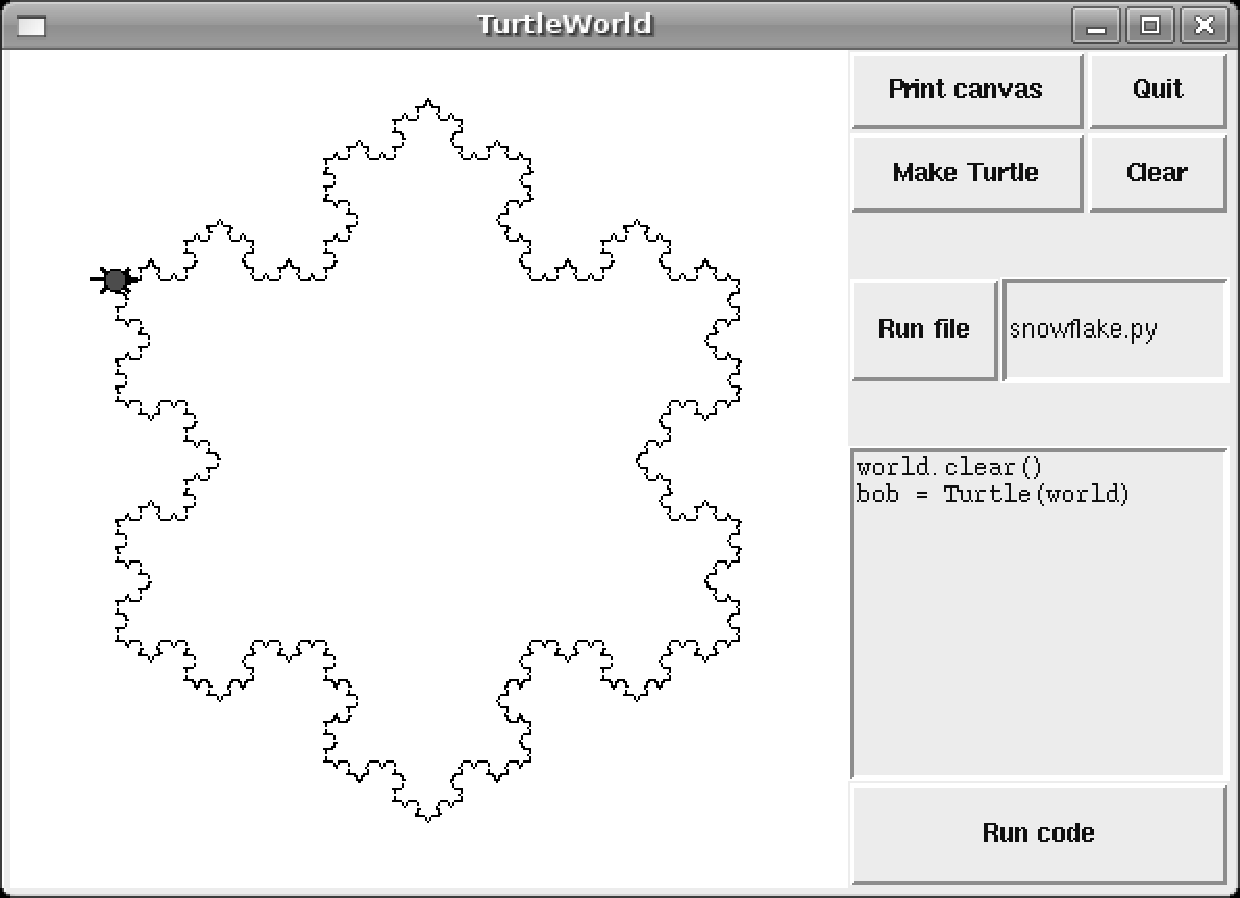
\includegraphics[scale=0.5]{figs/TurtleWorld.pdf}}
 \caption{Διάγραμμα κλάσεων.} 
\label{fig.turtleworld}
\end{figure}


 Σε αυτήν την ενότητα παρουσιάζεται ο κώδικας που δημιουργεί αυτό το  GUI,  σπασμένος σε μια σειρά βημάτων.  Μπορείτε να κατεβάσετε ολόκληρο το παράδειγμα από εδώ : 
\url{http://thinkpython.com/code/SimpleTurtleWorld.py}.

Στο ανώτατο επίπεδο, αυτό το  GUI  περιέχει δύο γραφικά στοιχεία, έναν Καμβά και ένα Πλαίσιο, διατεταγμένα σε μια σειρά.  Άρα το πρώτο βήμα είναι να δημιουργήσουμε αυτήν τη 
σειρά.   
\index{SimpleTurtleWorld class}
\index{class!SimpleTurtleWorld}

\begin{verbatim}
class SimpleTurtleWorld(TurtleWorld):
    """This class is identical to TurtleWorld, but the code that
    lays out the GUI is simplified for explanatory purposes."""

    def setup(self):
        self.row()
        ...
\end{verbatim}
%
 Η  {\tt setup}  είναι η συνάρτηση που δημιουργεί και οργανώνει τα γραφικά στοιχεία. 
Η οργάνωση των στοιχείων σε ένα  GUI  ονομάζεται πακετάρισμα.
\index{packing widgets}
\index{widget, packing}
\index{Frame widget}
\index{widget!Frame}

Η  {\tt row}  δημιουργεί ένα πλαίσιο σειράς και το κάνει το  " τρέχον πλαίσιο ".   Όλα τα επόμενα γραφικά στοιχεία πακετάρονται σε μία σειρά, μέχρι να κλείσει αυτό το πλαίσιο ή να δημιουργηθεί ένα άλλο.

Αυτός είναι ο κώδικας που δημιουργεί τον καμβά και το πλαίσιο στήλης όπου κρατάει τα 
άλλα στοιχεία :

\begin{verbatim}
        self.canvas = self.ca(width=400, height=400, bg='white')
        self.col()
\end{verbatim}
%
 Το πρώτο στοιχείο στην στήλη είναι ένα πλαίσιο πλέγματος, το οποίο περιέχει τέσσερα 
κουμπιά διατεταγμένα ανά δύο :

\begin{verbatim}
        self.gr(cols=2)
        self.bu(text='Print canvas', command=self.canvas.dump)
        self.bu(text='Quit', command=self.quit)
        self.bu(text='Make Turtle', command=self.make_turtle)
        self.bu(text='Clear', command=self.clear)
        self.endgr()
\end{verbatim}
%
 Η  {\tt gr}  δημιουργεί ένα πλέγμα, με όρισμα τον αριθμό των στηλών.  
Τα στοιχεία διατάσσονται στο πλέγμα από τα αριστερά προς τα δεξιά και από πάνω προς τα 
κάτω.
\index{callback}
\index{bound method}
\index{method, bound}
\index{subject}

Το πρώτο κουμπί χρησιμοποιεί την  {\tt self.canvas.dump}  σαν επιστροφή κλήσης και το 
δεύτερο χρησιμοποιεί την  {\tt self.quit}.   Αυτές είναι {\bf δεσμευμένες μέθοδοι}, το οποίο σημαίνει ότι σχετίζονται με ένα συγκεκριμένο αντικείμενο.  Όταν γίνεται επίκλησή τους, 
επικαλούνται στο αντικείμενο.

Το επόμενο γραφικό στοιχείο μέσα στη στήλη είναι ένα πλαίσιο γραμμής το οποίο περιέχει 
ένα κουμπί και μία είσοδο :

\begin{verbatim}
        self.row([0,1], pady=30)
        self.bu(text='Run file', command=self.run_file)
        self.en_file = self.en(text='snowflake.py', width=5)
        self.endrow()
\end{verbatim}
%
 Το πρώτο όρισμα στην  {\tt row}  είναι μία λίστα από βάρη η οποία καθορίζει πόσος 
επιπλέον χώρος διατίθεται μεταξύ των γραφικών στοιχείων.  Η λίστα  {\tt [0,1]}  σημαίνει ότι όλος ο επιπλέον χώρος επιμερίζεται στο δεύτερο στοιχείο, το οποίο είναι η είσοδος  (Entry).   Αν τρέξετε αυτόν τον κώδικα και αυξήσετε το μέγεθος του παραθύρου, 
θα δείτε ότι η είσοδος μεγαλώνει αλλά το κουμπί όχι.

Η επιλογή  {\tt pady} " γεμίζει "  αυτήν τη γραμμή προς την κατεύθυνση $y$, 
προσθέτοντας 30 εικονοστοιχεία πάνω και κάτω.

Η  {\tt endrow}  περατώνει αυτήν τη γραμμή στοιχείων και άρα τα επόμενα στοιχεία 
πακετάρονται στο πλαίσιο στήλης.  Το  {\tt Gui.py}  κρατάει μία στοίβα από πλαίσια :


\begin{itemize}

\item  Όταν χρησιμοποιείτε τις  {\tt row}, {\tt col}  ή  {\tt gr}  για 
να δημιουργήσετε ένα πλαίσιο  (Frame),  πηγαίνει στην αρχή της στοίβας και γίνεται 
το τρέχον πλαίσιο.

\item Όταν χρησιμοποιείτε τις  {\tt endrow}, {\tt endcol}  ή  {\tt endgr}  για 
να κλείσετε ένα πλαίσιο, πηδάει έξω από τη στοίβα και το προηγούμενο πλαίσιο γίνεται τρέχον.

\end{itemize}

Η μέθοδος  \verb"run_file"  διαβάζει τα περιεχόμενα της εισόδου, τα χρησιμοποιεί σαν 
όνομα αρχείου, διαβάζει τα περιεχόμενα και τα περνάει στην  \verb"run_code".   Η  
{\tt self.inter}  είναι ένα αντικείμενο διερμηνέα  (Interpreter)  το οποίο ξέρει 
πως να πάρει μία συμβολοσειρά και να την εκτελέσει σαν κώδικα  Python.

\begin{verbatim}
    def run_file(self):
        filename = self.en_file.get()
        fp = open(filename)
        source = fp.read()
        self.inter.run_code(source, filename)
\end{verbatim}
%
 Τα τελευταία δύο γραφικά στοιχεία είναι ένα  Text  και ένα κουμπί  (Button):

\begin{verbatim}
        self.te_code = self.te(width=25, height=10)
        self.te_code.insert(END, 'world.clear()\n')
        self.te_code.insert(END, 'bob = Turtle(world)\n')

        self.bu(text='Run code', command=self.run_text)
\end{verbatim}
%
 Η  \verb"run_text"  παρόμοια με την  \verb"run_file"  με τη διαφορά ότι 
παίρνει κώδικα από το στοιχείο  Text  αντί από ένα αρχείο :

\begin{verbatim}
    def run_text(self):
        source = self.te_code.get(1.0, END)
        self.inter.run_code(source, '<user-provided code>')
\end{verbatim}
%
 Δυστυχώς, οι λεπτομέρειες της διάταξης ενός γραφικού στοιχείου είναι διαφορετικές σε άλλες 
γλώσσες και στα άλλα αρθρώματα της  Python.   Μόνο το  Tkinter  παρέχει τρεις διαφορετικούς μηχανισμούς για την οργάνωση των στοιχείων.  Αυτοί οι μηχανισμοί ονομάζονται 
{\bf διαχειριστές γεωμετρίας}.  Αυτός που έδειξα σε αυτήν την ενότητα είναι ο  ``grid''  και οι άλλοι δύο ονομάζονται  ``pack''  και  ``place''.
\index{geometry manager}

 Ευτυχώς, οι περισσότερες έννοιες αυτής της ενότητας εφαρμόζονται και σε άλλα αρθρώματα 
γραφικής διασύνδεσης και άλλες γλώσσες.



\section{Μενού και αντικείμενα με δυνατότητα κλήσης}
\index{Menubutton widget}
\index{widget!Menubutton}

Ένα κουμπί μενού  (Menubutton)  είναι ένα γραφικό στοιχείο που μοιάζει με ένα απλό 
κουμπί, αλλά όταν πατηθεί αναδύεται ένα μενού.  Το μενού εξαφανίζεται όταν ο χρήστης επιλέξει 
από τα στοιχεία του.

Αυτός ο κώδικας δημιουργεί ένα έγχρωμο μενού επιλογών  ( μπορείτε να το κατεβάσετε από  \url{http://thinkpython.com/code/menubutton_demo.py}):

\begin{verbatim}
g = Gui()
g.la('Select a color:')
colors = ['red', 'green', 'blue']
mb = g.mb(text=colors[0])
\end{verbatim}
%
 Η  {\tt mb}  δημιουργεί ένα κουμπί μενού.  Αρχικά, το κείμενο στο κουμπί είναι το 
όνομα του προεπιλεγμένου χρώματος.  Ο ακόλουθος βρόχος δημιουργεί τα στοιχεία του μενού, ένα 
για κάθε χρώμα : 

\begin{verbatim}
for color in colors:
    g.mi(mb, text=color, command=Callable(set_color, color))
\end{verbatim}
%
 Το πρώτο όρισμα της  {\tt mi}  είναι το κουμπί μενού με το οποίο σχετίζονται 
αυτά τα στοιχεία.
\index{callback}
\index{Callable object}
\index{object!Callable}

Η επιλογή  {\tt command}  είναι ένα αντικείμενο με δυνατότητα κλήσης, το οποίο είναι 
κάτι νέο.  Μέχρι στιγμής έχουμε δει συναρτήσεις και μεθόδους οριοθέτησης να χρησιμοποιούνται 
σαν επιστροφές κλήσεων, το οποίο δουλεύει μια χαρά αν δεν χρειάζεται να περάσετε κάποιο όρισμα 
στη συνάρτηση.  Σε αντίθετη περίπτωση, πρέπει να κατασκευάσετε ένα αντικείμενο με δυνατότητα 
επιστροφής κλήσης  (Callable object)  το οποίο θα περιέχει μία συνάρτηση, όπως η  
\verb"set_color",  και τα ορίσματά της, όπως το  {\tt color}.

 Αυτό το αντικείμενο αποθηκεύει μία αναφορά στη συνάρτηση και τα ορίσματα σαν ιδιότητες.  
Αργότερα, όταν ο χρήστης κλικάρει σε ένα στοιχείο του μενού, η επιστρεφόμενη κλήση καλεί τη 
συνάρτηση και περνάει τα αποθηκευμένα ορίσματα.

Η  \verb"set_color"  θα μπορούσε να είναι αυτή :

\begin{verbatim}
def set_color(color):
    mb.config(text=color)
    print color
\end{verbatim}
%
 Όταν ο χρήστης επιλέξει ένα στοιχείο από το μενού, καλείται η  \verb"set_color",    
διαμορφώνει το κουμπί του μενού ούτως ώστε να δείχνει το νέο-επιλεγμένο χρώμα και στη 
συνέχεια το εμφανίζει.  Αν δοκιμάσετε να τρέξετε αυτό το παράδειγμα, μπορείτε να επιβεβαιώσετε 
ότι η  \verb"set_color"  καλείται όταν επιλέγετε ένα στοιχείο (και όχι όταν δημιουργείται το αντικείμενο  Callable ).



\section{Δεσμοί}
\index{binding}
\index{callback}

Ένας {\bf δεσμός} (binding) είναι μία σχέση μεταξύ ενός γραφικού στοιχείου, ενός 
συμβάντος και μιας επιστροφής κλήσης :  όταν προκληθεί ένα συμβάν (όπως το πάτημα ενός 
κουμπιού), επικαλείται η επιστροφή κλήσης.  

Πολλά γραφικά στοιχεία έχουν προεπιλεγμένους δεσμούς.  Για παράδειγμα, όταν πατάτε ένα 
κουμπί, ο προεπιλεγμένος δεσμός αλλάζει το ανάγλυφο του κουμπιού και το κάνει να φαίνεται 
κάπως μελαγχολικό.  Όταν αφήνετε το κουμπί, ο δεσμός επαναφέρει την εμφάνιση του και επικαλείται 
την επιστροφή κλήσης που καθορίζεται από την επιλογή  {\tt command}.

 Μπορείτε να χρησιμοποιήσετε την μέθοδο  {\tt bind}  για να παρακάμψετε τους προεπιλεγμένους δεσμούς ή για να προσθέσετε νέους.  Για παράδειγμα, αυτός ο κώδικας δημιουργεί 
ένα νέο δεσμό για έναν καμβά (μπορείτε να κατεβάσετε τον κώδικα αυτής της ενότητας από εδώ   \url{http://thinkpython.com/code/draggable_demo.py}):

\begin{verbatim}
ca.bind('<ButtonPress-1>', make_circle)
\end{verbatim}
%
 Το πρώτο όρισμα είναι μία συμβολοσειρά συμβάντος, το οποίο ενεργοποιείται όταν ο χρήστης 
πατήσει το αριστερό κουμπί του ποντικιού.  Άλλα συμβάντα του ποντικιού είναι το  {\tt ButtonMotion},  το  {\tt ButtonRelease}  και το  {\tt Double-Button}.
\index{event string}
\index{event handler}

 Το δεύτερο όρισμα είναι ένας χειριστής συμβάντων.  Ένας χειριστής συμβάντων είναι μία 
συνάρτηση ή μία μέθοδος οριοθέτησης, όπως μία επιστροφή κλήσης, αλλά με τη διαφορά 
ότι ένας χειριστής παίρνει ένα αντικείμενο συμβάντος σαν παράμετρο.  Αυτό είναι ένα 
παράδειγμα :

\begin{verbatim}
def make_circle(event):
    pos = ca.canvas_coords([event.x, event.y])
    item = ca.circle(pos, 5, fill='red')
\end{verbatim}
%
 Το αντικείμενο συμβάντος περιέχει πληροφορίες σχετικά με τον τύπο του συμβάντος και λεπτομέρειες όπως οι συντεταγμένες του δείκτη του ποντικιού.  Σε αυτό το παράδειγμα η πληροφορία που χρειαζόμαστε είναι η θέση του κλικ του ποντικιού.  Αυτές οι τιμές είναι 
συντεταγμένες σε εικονοστοιχεία, οι οποίες καθορίζονται από το γραφικό υποσύστημα.  Η μέθοδος 
 \verb"canvas_coords"  τις μετατρέπει σε συντεταγμένες καμβά, οι οποίες είναι συμβατές 
με τις μεθόδους του καμβά όπως η  {\tt circle}.
\index{Event object}
\index{object!Event}

Για τα γραφικά στοιχεία εισόδου, συνηθίζεται να δεσμεύουμε το συμβάν  \verb"<Return>", 
το οποίο ενεργοποιείται όταν ο χρήστης πατάει το πλήκτρο  {\sf Return}  ή το 
{\sf Enter}.  Για παράδειγμα, ο ακόλουθος κώδικας δημιουργεί ένα κουμπί  (Button)  και μία είσοδο (Entry):

\begin{verbatim}
bu = g.bu('Make text item:', make_text)
en = g.en()
en.bind('<Return>', make_text)
\end{verbatim}
%
 Η  \verb"make_text"  καλείται όταν πατιέται το κουμπί ή όταν ο χρήστης πατήσει 
το  {\sf Return}  ενώ πληκτρολογεί στην είσοδο.  Για να το κάνουμε να δουλέψει, χρειαζόμαστε μία συνάρτηση η οποία θα μπορεί να καλεστεί σαν επιλογή (χωρίς ορίσματα) ή 
σαν ένας χειριστής συμβάντος (με ένα συμβάν σαν όρισμα) :

\begin{verbatim}
def make_text(event=None):
    text = en.get()
    item = ca.text([0,0], text)
\end{verbatim}
%
 Η  \verb"make_text"  παίρνει τα περιεχόμενα της εισόδου και το κείμενό της σε ένα 
στοιχείο  Text  στον καμβά.

Επίσης, μπορούμε να δημιουργήσουμε δεσμούς για τα στοιχεία του καμβά.  Ακολουθεί ένας 
ορισμός για την κλάση  {\tt Draggable},  η οποία είναι παιδί της κλάσης  {\tt Item} 
 η οποία παρέχει δεσμούς οι οποίοι υλοποιούν τη δυνατότητα να σύρουμε και να αφήσουμε  (drag-and-drop).
\index{drag-and-drop}

\begin{verbatim}
class Draggable(Item):

    def __init__(self, item):
        self.canvas = item.canvas
        self.tag = item.tag
        self.bind('<Button-3>', self.select)
        self.bind('<B3-Motion>', self.drag)
        self.bind('<Release-3>', self.drop)
\end{verbatim}
%
 Η μέθοδος  init  παίρνει ένα στοιχείο σαν παράμετρο, αντιγράφει τις ιδιότητές του και στη συνέχεια δημιουργεί δεσμούς για τρία συμβάντα :  το πάτημα του κουμπιού, την κίνηση του κουμπιού και την ελευθέρωσή του.

Ο χειριστής συμβάντων  {\tt select}  αποθηκεύει τις συντεταγμένες του τρέχοντος συμβάντος και το αρχικό χρώμα του στοιχείου και στη συνέχεια αλλάζει το χρώμα σε κίτρινο :

\begin{verbatim}
    def select(self, event):
        self.dragx = event.x
        self.dragy = event.y

        self.fill = self.cget('fill')
        self.config(fill='yellow')
\end{verbatim}
%
 Το  {\tt cget}  σημαίνει  ``get configuration''.   Παίρνει αυτό το όνομα από 
μία επιλογή σαν συμβολοσειρά και επιστρέφει την τρέχουσα τιμή αυτής της επιλογής.

Η  {\tt drag}  υπολογίζει πόσο μακριά μετακινήθηκε το αντικείμενο σε σχέση με την 
αρχική του θέση, ενημερώνει τις αποθηκευμένες συντεταγμένες και στη συνέχεια μετακινεί το 
στοιχείο. 
\index{update!coordinate}

\begin{verbatim}
    def drag(self, event):
        dx = event.x - self.dragx
        dy = event.y - self.dragy

        self.dragx = event.x
        self.dragy = event.y

        self.move(dx, dy)
\end{verbatim}
%
 Αυτός ο υπολογισμός γίνεται σε συντεταγμένες εικονοστοιχείων (δεν υπάρχει λόγος να μετατραπούν σε συντεταγμένες καμβά).
\index{Canvas coordinate}
\index{coordinate!Canvas}
\index{pixel coordinate}
\index{coordinate!pixel}

Τέλος, η  {\tt drop}  επαναφέρει το αρχικό χρώμα του στοιχείου :

\begin{verbatim}
    def drop(self, event):
        self.config(fill=self.fill)
\end{verbatim}
%
 Μπορείτε να χρησιμοποιήσετε την κλάση  {\tt Draggable}  για προσθέσετε δυνατότητα 
 drag-and-drop  σε ένα υπάρχον στοιχείο.  Για παράδειγμα, αυτή είναι μία τροποποιημένη 
έκδοση της  \verb"make_circle"  η οποία χρησιμοποιεί την  {\tt circle}  για να 
δημιουργήσει ένα στοιχείο και την  {\tt Draggable}  για να το κάνει 
 " συρόμενο ":

\begin{verbatim}
def make_circle(event):
    pos = ca.canvas_coords([event.x, event.y])
    item = ca.circle(pos, 5, fill='red')
    item = Draggable(item)
\end{verbatim}
%
 Αυτό το παράδειγμα επιδεικνύει ένα από τα πλεονεκτήματα της κληρονομικότητας :  
μπορείτε να τροποποιήσετε της δυνατότητες μίας γονικής κλάσης χωρίς να τροποποιήσετε τον ορισμό της.  Αυτό είναι ιδιαίτερα χρήσιμο αν θέλετε να αλλάξετε τη συμπεριφορά που ορίζεται 
σε ένα άρθρωμα που δεν γράψατε εσείς.



\section{Αποσφαλμάτωση}
\index{debugging}

Μία από τις προκλήσεις του προγραμματισμού με γραφική διασύνδεση είναι η παρακολούθηση του τι 
συμβαίνει όταν χτίζεται το  GUI  και του τι γίνεται αργότερα ως απόκριση στις ενέργειες του χρήστη.  
\index{callback}

Για παράδειγμα, είναι σύνηθες λάθος όταν φτιάχνετε μία επιστροφή κλήσης να καλείτε την συνάρτηση αντί να περνάτε μία αναφορά σε αυτήν :

\begin{verbatim}
def the_callback():
    print 'Called.'

g.bu(text='This is wrong!', command=the_callback())
\end{verbatim}
%
 Αν τρέξετε αυτόν τον κώδικα, θα δείτε ότι καλεί την  \verb"the_callback"  αμέσως, 
και στη συνέχεια δημιουργεί ένα κουμπί.  Όταν πατάτε το κουμπί, δεν κάνει τίποτα επειδή η επιστρεφόμενη τιμή της  \verb"the_callback"  είναι  {\tt None}.   
Δεν θα θέλατε να επικαλεστείτε μία επιστροφή κλήσης κατά την ανάπτυξη ενός  GUI  αλλά 
μόνο μετά, σαν απόκριση σε μία ενέργεια του χρήστη.
\index{flow of execution}
\index{event-driven programming}

Μία άλλη πρόκληση του προγραμματισμού με γραφική διασύνδεση είναι ότι δεν έχετε τον έλεγχο 
της ροής εκτέλεσης.  Οι ενέργειες του χρήστη καθορίζουν ποια τμήματα του κώδικα θα εκτελεστούν 
και με ποια σειρά.  Αυτό σημαίνει ότι πρέπει να σχεδιάσετε το πρόγραμμά σας με τέτοιο τρόπο ούτως ώστε να δουλεύει σωστά με οποιαδήποτε πιθανή σειρά συμβάντων.

Για παράδειγμα, το  GUI  της άσκησης~ \ref{circle2}  έχει δύο γραφικά στοιχεία :  το ένα δημιουργεί ένα στοιχείο  Circle  και το άλλο αλλάζει το χρώμα του κύκλου.  Αν ο χρήστης δημιουργήσει τον κύκλο και στη συνέχεια αλλάξει το χρώμα του δεν υπάρχει κανένα πρόβλημα.  Αλλά αν ο χρήστης αλλάξει το χρώμα ενός κύκλου που δεν υπάρχει ακόμα ;   Ή δημιουργήσει περισσότερους του ενός κύκλου ;

 Όσο αυξάνεται ο αριθμός των γραφικών στοιχείων, γίνεται όλο και πιο δύσκολο να φανταστούμε 
όλες τις πιθανές σειρές συμβάντων.  Ένας τρόπος για να χειριστούμε αυτήν την πολυπλοκότητα είναι να ενθυλακώσουμε την κατάσταση του συστήματος σε ένα αντικείμενο και στη συνέχεια να εξετάσουμε :

\begin{itemize}

 
\item Ποιες είναι οι πιθανές καταστάσεις ;   Στο παράδειγμα με τον κύκλο, θα πρέπει 
να εξετάσουμε δύο καταστάσεις :  πριν και μετά τη δημιουργία του πρώτου κύκλου από το 
χρήστη.

\item Σε κάθε κατάσταση, ποια συμβάντα μπορεί να προκύψουν;  Στο παράδειγμα, ο χρήστης 
μπορεί να πατήσει οποιοδήποτε από τα κουμπιά ή να το κλείσει.

\item Για κάθε ζευγάρι κατάστασης-συμβάντος, ποιο είναι το επιθυμητό αποτέλεσμα ;   
Από τη στιγμή που υπάρχουν δύο καταστάσεις και δύο κουμπιά, υπάρχουν τέσσερα ζευγάρια κατάστασης-συμβάντος που πρέπει να εξεταστούν.

\item Τι μπορεί να προκαλέσει μία μετάβαση από μία κατάσταση σε μία άλλη ;   
Σε αυτήν την περίπτωση, υπάρχει μία μετάβαση όταν ο χρήστης δημιουργεί τον πρώτο κύκλο.
 

\end{itemize}

 Επίσης, μπορεί να σας φανεί χρήσιμο να ορίσετε και να ελέγξετε σταθερές οι οποίες θα 
κρατάνε ανεξάρτητα τη σειρά των συμβάντων.
\index{invariant}

Αυτή η προσέγγιση στον προγραμματισμό με διασύνδεση χρήστη μπορεί να σας βοηθήσει να γράψετε 
σωστό κώδικα χωρίς να αφιερώσετε χρόνο στον έλεγχο κάθε πιθανής ακολουθίας συμβάντων !



 
\section{Ορολογία}

\begin{description} 

\item[GUI:]  Μία γραφική διασύνδεση χρήστη. 
\index{GUI}

\item[widget:]  Ένα από τα γραφικά στοιχεία που συνθέτουν μία γραφική διασύνδεση χρήστη, 
συμπεριλαμβανομένων κουμπιών, μενού, πεδία εισαγωγής κειμένου κτλ.
\index{widget}

\item[επιλογή:] Μία τιμή η οποία ρυθμίζει την εμφάνιση ή τη συνάρτηση ενός γραφικού στοιχείου.
\index{option}

\item[όρισμα λέξη κλειδί:] Ένα όρισμα το οποίο υποδεικνύει το όνομα της παραμέτρου σαν μέρος 
της κλήσης συνάρτησης.
\index{keyword argument}

\item[επιστροφή κλήσης:] Μία συνάρτηση συσχετισμένη με ένα  widget  η οποία καλείται 
όταν ο χρήστης εκτελεί μία ενάργεια.
\index{callback}

\item[μέθοδος οριοθέτησης:] Μία μέθοδος η οποία σχετίζεται με ένα συγκεκριμένο στιγμιότυπο.
\index{bound method}

\item[προγραμματισμός βάση συμβάντων:] Ένα είδος προγραμματισμού στο οποίο η ροή της εκτέλεσης 
καθορίζεται από τις ενέργειες του χρήστη.
\index{event-driven programming}

\item[συμβάν:] Μία ενέργεια του χρήστη, όπως το κλικ του ποντικιού ή το πάτημα ενός κουμπιού, 
η οποία προκαλεί την απόκριση του  GUI. 
\index{event}

\item[βρόχος συμβάντων:] Ένας ατέρμον βρόχος ο οποίος περιμένει τις ενέργειες του χρήστη και 
αποκρίνεται.
\index{event loop}

\item[στοιχείο:] Ένα γραφικό στοιχείο σε ένα  widget  καμβά.
\index{item!Canvas}

\item[πλαίσιο οριοθέτησης:] Ένα ορθογώνιο παραλληλόγραμμο το οποίο περικλείει ένα σύνολο 
στοιχείων, συνήθως καθορισμένα από δύο απέναντι γωνίες.
\index{bounding box}

\item[πακέτο:] Για την οργάνωση και εμφάνιση των στοιχείων ενός  GUI. 
\index{packing widgets}

\item[διαχειριστής γεωμετρίας:] Ένα σύστημα για το πακετάρισμα γραφικών στοιχείων.
\index{geometry manager}

\item[δεσμός:] Μία συσχέτιση μεταξύ ενός γραφικού στοιχείου, ενός συμβάντος και ενός χειριστή συμβάντων.  Ο χειριστής συμβάντων καλείται όταν προκύψει ένα συμβάν σε ένα γραφικό στοιχείο.
\index{binding}

\end{description}


\section{Ασκήσεις}

\begin{exercise}
\index{image viewer}

Για αυτήν την άσκηση θα γράψετε ένα πρόγραμμα προβολής εικόνων.  Αυτό είναι ένα απλό παράδειγμα :

\begin{verbatim}
g = Gui()
canvas = g.ca(width=300)
photo = PhotoImage(file='danger.gif')
canvas.image([0,0], image=photo)
g.mainloop()
\end{verbatim}
%
 Η  {\tt PhotoImage}  διαβάζει ένα αρχείο και επιστρέφει ένα αντικείμενο  {\tt PhotoImage}  το οποίο μπορεί να εμφανίσει το  Tkinter.   Η  {\tt Canvas.image}  τοποθετεί την εικόνα στον καμβά, κεντραρισμένη στις δοθείσες συντεταγμένες.  Μπορείτε επίσης να βάλετε εικόνες και πάνω σε ετικέτες, κουμπιά και κάποια άλλα γραφικά στοιχεία :

\begin{verbatim}
g.la(image=photo)
g.bu(image=photo)
\end{verbatim}
%
 Η  PhotoImage  μπορεί να χειριστεί μόνο μερικούς τύπους εικόνας, όπως τον  GIF  και τον  PPM,  αλλά μπορούμε να χρησιμοποιήσουμε την βιβλιοθήκη εικόνων της  Python (PIL)  για να διαβάσουμε και άλλα αρχεία.
\index{Python Imaging Library (PIL)}
\index{PIL (Python Imaging Library)}
\index{Image module}
\index{module!Image}

Το όνομα του αρθρώματος  PIL  είναι  {\tt Image},  αλλά το  Tkinter  ορίζει 
ένα αντικείμενο με το ίδιο όνομα.  Για να αποφευχθεί η σύγκρουση, μπορείτε να χρησιμοποιήσετε την  {\tt import...as}  με αυτόν τον τρόπο :

\begin{verbatim}
import Image as PIL
import ImageTk
\end{verbatim}
%
 Η πρώτη γραμμή εισάγει το  {\tt Image}  και του δίνει το τοπικό όνομα  {\tt PIL}.   Η δεύτερη γραμμή εισάγει το  {\tt ImageTk},  το οποίο μπορεί να μεταφράσει 
μία εικόνα  PIL  σε ένα  Tkinter PhotoImage.   Για παράδειγμα :

\begin{verbatim}
image = PIL.open('allen.png')
photo2 = ImageTk.PhotoImage(image)
g.la(image=photo2)
\end{verbatim}
%

 
\begin{enumerate}

\item Κατεβάστε τα \verb"image_demo.py", \verb"danger.gif" και \verb"allen.png" από εδώ \url{http://thinkpython.com/code}. Τρέξτε το  \verb"image_demo.py". Ίσως χρειαστεί να εγκαταστήσετε τα {\tt PIL} και {\tt ImageTk}.  Θα τα βρείτε πιθανώς στις αποθήκες λογισμικού, αλλά αν όχι τότε μπορείτε να τα κατεβάσετε από το 
σύνδεσμο \url{pythonware.com/products/pil/}. 

\item Στο \verb"image_demo.py"  αλλάξτε το όνομα του δεύτερου  PhotoImage  από 
 {\tt photo2}  σε  {\tt photo}  και ξανατρέξτε το πρόγραμμα.  Θα πρέπει να δείτε το δεύτερο  PhotoImage  αλλά όχι το πρώτο.

Το πρόβλημα είναι ότι όταν επανεκχωρείτε την  {\tt photo}  παρακάμπτεται η αναφορά στο 
πρώτο  PhotoImage,  το οποίο στη συνέχεια εξαφανίζεται.  Το ίδιο συμβαίνει και αν εκχωρήσετε ένα  PhotoImage  σε μια τοπική μεταβλητή, εξαφανίζεται με το τέλος της συνάρτησης.

Για να αποφύγετε αυτό το πρόβλημα, πρέπει να αποθηκεύσετε μία αναφορά σε κάθε  PhotoImage  που θέλετε να κρατήσετε.  Μπορείτε να χρησιμοποιήσετε μία καθολική μεταβλητή ή να αποθηκεύσετε τα  PhotoImages  σε δομές δεδομένων ή σαν μία ιδιότητα ενός αντικειμένου.

Αυτή η συμπεριφορά μπορεί είναι απογοητευτική, για αυτό σας προειδοποιώ (και για αυτό η εικόνα του παραδείγματος λέει  ``Danger!'' ).
\index{bug!worst ever}
\index{worst bug!ever}

\item Γράψτε ένα πρόγραμμα βασισμένοι σε αυτό το παράδειγμα, το οποίο θα παίρνει το όνομα 
ενός καταλόγου και θα διέρχεται μέσω όλων των αρχείων, εμφανίζοντας τα αρχεία που η το  PIL 
 αναγνωρίζει σαν εικόνες.  Μπορείτε να χρησιμοποιήσετε μία δήλωση  {\tt try}  για να πιάσετε τα αρχεία που δεν αναγνωρίζει το  PIL. 

Όταν ο χρήστης κάνει κλικ πάνω στην εικόνα, το πρόγραμμα θα πρέπει να εμφανίζει την επόμενη.

\item Το  PIL  παρέχει διάφορες μεθόδους για τον χειρισμό εικόνων.  
Μπορείτε να διαβάσετε σχετικά με αυτό στο σύνδεσμο  \url{http://pythonware.com/library/pil/handbook}.  
Σαν πρόκληση, διαλέξτε μερικές από αυτές τις μεθόδους και δημιουργήστε ένα  GUI  για 
να τις εφαρμόσετε σε εικόνες.

\end{enumerate}

Λύση : \url{http://thinkpython.com/code/ImageBrowser.py}.

\end{exercise}



\begin{exercise}
\index{vector graphics}
\index{SVG}

Ένας επεξεργαστής διανυσματικών γραφικών είναι ένα πρόγραμμα το οποίο δίνει στους χρήστες 
τη δυνατότητα να σχεδιάσουν και να επεξεργαστούν σχήματα στην οθόνη και να δημιουργήσουν αρχεία εξόδου σε τύπους διανυσματικών γραφικών όπως το  Postscript  και το  SVG.

 Γράψτε έναν απλό επεξεργαστή διανυσματικών γραφικών χρησιμοποιώντας το  Tkinter.   
Θα πρέπει, τουλάχιστον, να επιτρέπει στους χρήστες να σχεδιάσουν γραμμές, κύκλους και ορθογώνια.  Χρησιμοποιήστε την  {\tt Canvas.dump}  για παράγετε το σχετικό  Postscript  των περιεχομένων του καμβά.

Σαν πρόκληση, μπορείτε να επιτρέψετε τους χρήστες να επιλέγουν και να αλλάζουν το μέγεθος 
των στοιχείων του καμβά. 

% TODO: write a solution!

\end{exercise}



\begin{exercise}

Χρησιμοποιήστε το  Tkinter  για να γράψετε ένα απλό περιηγητή ιστού.  Θα πρέπει να 
έχει ένα γραφικό στοιχείο  Text  όπου ο χρήστης θα μπορεί να εισάγει ένα  URL  και 
ένα  Canvas  για να δείχνει τα περιεχόμενα της σελίδας.
\index{urllib module}
\index{module!urllib}
\index{URL}
\index{HTMLParser module}
\index{module!HTMLParser}

Μπορείτε να χρησιμοποιήσετε το άρθρωμα  {\tt urllib}  για να κατεβάσετε αρχεία (βλ. άσκηση~ \ref{urllib})  και το άρθρωμα  {\tt HTMLParser}  για την ανάλυση των  
HTML tags  (δείτε εδώ  \url{http://docs.python.org/2/library/htmlparser.html}).
\index{plain text}
\index{text!plain}
\index{hyperlink}

 Κατ'ελάχιστο, ο περιηγητής σας θα πρέπει να χειρίζεται απλό κείμενο και υπερσυνδέσμους.  Σαν πρόκληση μπορείτε να χειριστείτε χρώματα φόντου, διαμόρφωση ετικετών και εικόνων.

% TODO: write a solution!
\end{exercise}




\appendix

\chapter{Αποσφαλμάτωση}

\index{debugging}
Σε ένα πρόγραμμα μπορούν να συμβούν διαφόρων ειδών σφάλματα και είναι χρήσιμο 
να γίνει διάκριση μεταξύ τους προκειμένου να μπορούμε να τα εντοπίσουμε γρηγορότερα :

\begin{itemize}

\item  Τα συντακτικά λάθη παράγονται από την  Python  όταν μεταφράζει τον πηγαίο 
  κώδικα σε  byte code  (όχι γλώσσα μηχανής).  Συνήθως, υποδεικνύουν ότι υπάρχει κάποιο 
  λάθος στη σύνταξη του προγράμματος.  Παράδειγμα :   Η παράλειψη της άνω κάτω τελείας 
  στο τέλος μίας δήλωσης  {\tt def}  αποδίδει το κάπως περιττό μήνυμα  
  {\tt SyntaxError: invalid syntax}.

\item  Τα λάθη χρόνου εκτέλεσης παράγονται από τον διερμηνέα αν πάει κάτι στραβά κατά την 
  εκτέλεση του προγράμματος.  Τα περισσότερα μηνύματα αυτών των σφαλμάτων περιέχουν 
  πληροφορίες σχετικά με το που συνέβη το σφάλμα και τι συναρτήσεις εκτελούνταν. 
  Παράδειγμα :  Μία άπειρη αναδρομή, τελικώς, θα προκαλέσει το σφάλμα χρόνου εκτέλεσης 
   ``maximum recursion depth exceeded.''

\item  Τα σημασιολογικά λάθη είναι αποτελούν προβλήματα σε ένα πρόγραμμα το οποίο τρέχει 
  χωρίς να παράγει κάποιο μήνυμα λάθους αλλά δεν κάνει αυτό που θα έπρεπε.  Παράδειγμα : 
   Μία έκφραση μπορεί να μην υπολογίζεται με τη σειρά που θα περιμένατε, αποδίδοντας 
  ένα εσφαλμένο αποτέλεσμα. 

\end{itemize}
\index{syntax error}
\index{runtime error}
\index{semantic error}
\index{error!compile-time}
\index{error!syntax}
\index{error!runtime}
\index{error!semantic}
\index{exception}

 Το πρώτο βήμα της αποσφαλμάτωσης είναι να καταλάβετε με τι είδους λάθος έχετε να κάνετε.  
Παρόλο που οι ακόλουθες ενότητες είναι οργανωμένες με βάση τον τύπο του σφάλματος, μερικές τεχνικές μπορούν να εφαρμοστούν σε περισσότερες από μία περιπτώσεις.


\section{Συντακτικά λάθη}
\index{error message}

Συνήθως, τα συντακτικά λάθη είναι εύκολο να διορθωθούν από τη στιγμή που καταλάβετε ποια 
είναι.  Δυστυχώς, τις περισσότερες φορές τα μηνύματα λάθους δεν είναι και πολύ χρήσιμα. 
Τα συνηθέστερα μηνύματα είναι το  {\tt SyntaxError: invalid syntax}  και το  
{\tt SyntaxError: invalid token},  εκ των οποίων κανένα δεν είναι ιδιαίτερα κατατοπιστικό. 

Αφετέρου, το μήνυμα σας λέει που συνέβη το σφάλμα μέσα στο πρόγραμμα.  Για την ακρίβεια, σας 
λέει που παρατήρησε το πρόβλημα η  Python,  το οποίο δεν είναι απαραίτητα και το που ακριβώς είναι το λάθος.  Μερικές φορές το λάθος είναι πριν τη θέση του μηνύματος λάθους. 
Συνήθως είναι στην αμέσως προηγούμενη γραμμή.
\index{incremental development}
\index{development plan!incremental}

Εάν χτίζετε σταδιακά το πρόγραμμα, τότε μάλλον γνωρίζεται που είναι το λάθος. Θα είναι στην 
τελευταία γραμμή που προσθέσατε.

Αν αντιγράφετε κώδικα από ένα βιβλίο, ξεκινήστε συγκρίνοντας πολύ προσεκτικά τον κώδικά σας με 
αυτόν του βιβλίου.  Ελέγξτε κάθε χαρακτήρα.  Συγχρόνως, θυμηθείτε ότι μπορεί να είναι λάθος το 
βιβλίο, επομένως αν δείτε κάτι που μοιάζει με συντακτικό λάθος τότε μπορεί και να είναι.

Αυτοί είναι μερικοί τρόποι για να αποφύγετε τα πιο συνηθισμένα συντακτικά λάθη :
\index{syntax}

\begin{enumerate}

\item  Σιγουρευτείτε ότι δεν χρησιμοποιείτε κάποια λέξη κλειδί σαν όνομα μεταβλητής. 
\index{keyword}

\item  Ελέγξτε ότι έχετε άνω και κάτω τελεία στο τέλος της επικεφαλίδας κάθε σύνθετης 
δήλωσης, συμπεριλαμβανομένων των  {\tt for}, {\tt while}, {\tt if},  και  {\tt def}.
\index{header}
\index{colon}

\item  Σιγουρευτείτε ότι όλες οι συμβολοσειρές μέσα στον κώδικα έχουν σωστές αντιστοιχίες  εισαγωγικών. 
\index{quotation mark}

\item  Αν έχετε συμβολοσειρές πολλαπλών γραμμών με τριπλά εισαγωγικά (μονά ή διπλά), σιγουρευτείτε ότι τερματίσατε κατάλληλα τη συμβολοσειρά.  Μία μη τερματισμένη συμβολοσειρά 
μπορεί να προκαλέσει ένα λάθος  {\tt invalid token}  στο τέλος του προγράμματος, ή μπορεί να χειριστεί το υπόλοιπο μέρος του προγράμματος σαν μία συμβολοσειρά μέχρι να φτάσει 
στην επόμενη συμβολοσειρά.  Στην δεύτερη περίπτωση, μπορεί να μην παραχθεί κανένα μήνυμα λάθους !
\index{multiline string}
\index{string!multiline}

\item  Ένας τελεστής ανοίγματος που δεν έχει κλείσει, όπως οι  \verb+(+, \verb+{+,  
  και  \verb+[+,  κάνει την  Python  να συνεχίσει στην επόμενη γραμμή σαν να ήταν       
  μέρος της τρέχουσας δήλωσης.  Σε γενικές γραμμές, θα προκύψει λάθος σχεδόν αμέσως στην 
  επόμενη γραμμή. 

\item  Ελέγξτε για το κλασικό  {\tt =}  αντί του  {\tt ==}  μέσα σε μία συνθήκη. 
\index{conditional}

\item  Ελέγξτε την ενδοπαραγραφοποίηση για να σιγουρευτείτε ότι ευθυγραμμίζονται με τον τρόπο που θα έπρεπε.  Η  Python  μπορεί να χειριστεί κενά διαστήματα και στηλοθέτες, 
αλλά αν τα ανακατέψετε μπορεί να προκαλέσετε προβλήματα.  Ο καλύτερος τρόπος για να αποφύγετε 
τέτοια προβλήματα είναι να χρησιμοποιείτε έναν κειμενογράφο που γνωρίζει την  Python  
και παράγει κατάλληλη ενδοπαραγραφοποίηση. 
\index{indentation}
\index{whitespace}

\end{enumerate}

 Αν δεν δουλέψει τίποτα από αυτά, προχωρήστε στην επόμενη ενότητα...


\subsection{Συνεχίζω να κάνω αλλαγές αλλά δεν υπάρχει διαφορά.}

Αν ο διερμηνέας λέει ότι υπάρχει ένα λάθος και εσείς δεν το βλέπετε, τότε μπορεί εσείς και 
ο διερμηνέας να κοιτάτε διαφορετικό κώδικα.  Ελέγξτε το προγραμματιστικό σας περιβάλλον για 
σιγουρευτείτε ότι το πρόγραμμα που επεξεργάζεστε είναι το ίδιο με αυτό που προσπαθεί να τρέξει 
η  Python.

 Αν δεν είστε σίγουροι, δοκιμάστε να βάλετε ένα προφανές συντακτικό λάθος στην αρχή του 
κώδικα σκόπιμα.  Τώρα ξανατρέξτε το.  Αν ο διερμηνέας δεν βρει το νέο λάθος, τότε δεν τρέχετε 
το νέο κώδικα.

Υπάρχουν κάποιοι πιθανοί ένοχοι :

\begin{itemize}

\item  Επεξεργαστήκατε το αρχείο και ξεχάσατε να αποθηκεύσετε τις αλλαγές πριν το ξανατρέξετε.  Μερικά προγραμματιστικά περιβάλλοντα το κάνουν αυτό από μόνα τους, αλλά κάποια 
άλλα όχι. 

\item  Αλλάξατε το όνομα του αρχείου αλλά προσπαθείτε να το τρέξετε με το παλιό όνομα. 

\item  Κάτι στο προγραμματιστικό σας περιβάλλον δεν έχει ρυθμιστεί σωστά. 

\item  Αν γράφετε ένα άρθρωμα και χρησιμοποιείτε την  {\tt import},  σιγουρευτείτε 
ότι δεν δώσατε στο άρθρωμά σας το ίδιο όνομα με ένα από τα πρότυπα αρθρώματα της  Python.
\index{module!reload}
\index{reload function}
\index{function!reload}

\item  Αν χρησιμοποιείτε την {\tt import} για να διαβάσετε ένα άρθρωμα, θυμηθείτε 
ότι πρέπει να επανεκκινήστε τον διερμηνέα ή να χρησιμοποιήσετε την {\tt reload} για να 
διαβάσετε ένα τροποποιημένο αρχείο.  Αν επανεισάγετε απλά το άρθρωμα, δεν θα κάνει κάτι. 

\end{itemize}

 Αν κολλήσετε και δεν μπορείτε να καταλάβετε τι συμβαίνει, μία προσέγγιση είναι να ξεκινήσετε από την αρχή με ένα νέο πρόγραμμα όπως το  ``Hello, World!''  και να σιγουρευτείτε ότι μπορείτε να τρέξετε ένα τέτοιο γνωστό πρόγραμμα.  Στη συνέχεια προσθέστε σταδιακά τα κομμάτια του αρχικού προγράμματος στο νέο.


\section{Λάθη χρόνου εκτέλεσης}

Από τη στιγμή που το πρόγραμμά σας είναι συντακτικά σωστό, η  Python  μπορεί να το 
μεταγλωττίσει και να αρχίσει τουλάχιστον να το τρέχει. Τι θα μπορούσε ενδεχομένως να πάει στραβά ;  


\subsection{Το πρόγραμμά μου δεν κάνει απολύτως τίποτα.}

Συνήθως, αυτό το πρόβλημα προκύπτει όταν το αρχείο σας αποτελείται από συναρτήσεις και 
κλάσεις αλλά στην πραγματικότητα δεν επικαλείται τίποτα για να αρχίσει η εκτέλεση.  
Αυτό μπορεί να είναι σκόπιμο αν σχεδιάζετε να εισάγεται αυτό το άρθρωμα για να παρέχετε 
κλάσεις και συναρτήσεις.

Αν δεν είναι σκόπιμο, σιγουρευτείτε ότι επικαλείστε μία συνάρτηση για να αρχίσει η εκτέλεση, 
ή εκτελέστε μία στην διαδραστική λειτουργία.  Δείτε επίσης και την ενότητα  " 
Ροή Εκτέλεσης "  παρακάτω.


\subsection{Το πρόγραμμά μου κρεμάει.}
\index{infinite loop}
\index{infinite recursion}
\index{hanging}

Αν ένα πρόγραμμα σταματήσει και φαίνεται να μην κάνει τίποτα, τότε λέμε ότι  " κρέμασε ".   Συχνά, αυτό σημαίνει ότι το έχει κολλήσει μέσα σε έναν ατέρμων βρόχο ή μία ατέρμονη αναδρομή. 

\begin{itemize}

\item Αν υποψιάζεστε ότι το πρόβλημα είναι ένας συγκεκριμένος βρόχος, προσθέστε 
μία δήλωση  {\tt print}  αμέσως πριν το βρόχο η οποία θα λέει  
``entering the loop''  και μία άλλη αμέσως μετά η οποία θα λέει  
``exiting the loop.''

 Δοκιμάστε να ξανατρέξετε το πρόγραμμα. Αν πάρετε το πρώτο μήνυμα αλλά όχι το 
δεύτερο τότε έχετε έναν ατέρμων βρόχο.  Πηγαίνετε στην ενότητα  " Ατέρμων Βρόχος "  παρακάτω.

\item Τις περισσότερες φορές, μία ατέρμονη αναδρομή θα αναγκάσει το πρόγραμμα να τρέξει για λίγο και στη συνέχεια θα παραχθεί ένα σφάλμα ``RuntimeError: Maximum recursion depth exceeded''. Αν συμβεί αυτό πηγαίνετε στην ενότητα "Ατέρμονη Αναδρομή" παρακάτω.

Ακόμα και αν δεν πάρετε αυτό το λάθος αλλά υποπτεύεστε ότι υπάρχει πρόβλημα με μία αναδρομική μέθοδο ή συνάρτηση, μπορείτε να χρησιμοποιήσετε τις ίδιες τεχνικές τις 
ενότητας  " Ατέρμονη Αναδρομή ". 

\item Αν δεν δουλέψει κανένα από τα παραπάνω βήματα, αρχίστε να ελέγχετε άλλους 
βρόχους και άλλες αναδρομικές συναρτήσεις και μεθόδους.

\item Αν δεν δουλέψει ούτε αυτό, τότε είναι πιθανό να μην έχετε καταλάβει τη ροή 
εκτέλεσης του προγράμματος.  Πηγαίνετε στην ενότητα  " Ροή Εκτέλεσης "  
παρακάτω.

\end{itemize}


\subsubsection{Ατέρμων Βρόχος}
\index{infinite loop}
\index{loop!infinite}
\index{condition}
\index{loop!condition}

Αν πιστεύετε ότι έχετε έναν ατέρμων βρόχο και νομίζετε ότι ξέρετε ποιος βρόχος προκαλεί το πρόβλημα, προσθέστε μία δήλωση  {\tt print}  στο τέλος του βρόχου, η οποία θα εμφανίζει τις τιμές των μεταβλητών μέσα στην συνθήκη και την τιμή της συνθήκης.

Για παράδειγμα :

\begin{verbatim}
while x > 0 and y < 0 :
    # do something to x
    # do something to y

    print "x: ", x
    print "y: ", y
    print "condition: ", (x > 0 and y < 0)
\end{verbatim}
%
 Τώρα, όταν τρέξετε το πρόγραμμα, θα δείτε τρεις γραμμές εξόδου για κάθε επανάληψη του βρόχου.  Στην τελευταία επανάληψη, η συνθήκη θα πρέπει να είναι ψευδής.  Αν ο βρόχος συνεχίσει να εκτελείται, θα είστε σε θέση να δείτε τις τιμές 
των  {\tt x}  και  {\tt y},  και μπορεί να καταλάβετε για ποιο λόγο δεν  ενημερώνονται σωστά.


\subsubsection{Ατέρμονη Αναδρομή}
\index{infinite recursion}
\index{recursion!infinite}

Τις περισσότερες φορές, μία ατέρμονη αναδρομή προκαλεί την εκτέλεση του προγράμματος για λίγο και στη συνέχεια παράγεται ένα σφάλμα  
{\tt Maximum recursion depth exceeded}.

 Αν υποψιάζεστε ότι μία συνάρτηση ή μία μέθοδος προκαλεί ατέρμονη αναδρομή, 
ξεκινήστε ελέγχοντας αν υπάρχει περίπτωση βάσης.  Με άλλα λόγια, θα πρέπει να 
υπάρχει μία συνθήκη η οποία θα αναγκάσει τη συνάρτηση ή τη μέθοδο να επιστρέψει 
χωρίς να κάνει αναδρομική επίκληση.  Αν όχι, τότε θα πρέπει να επανεξετάσετε τον 
αλγόριθμο και να προσδιορίσετε μία περίπτωση βάσης.

Αν υπάρχει περίπτωση βάσης αλλά το πρόγραμμα δεν φαίνεται να την φτάνει, προσθέστε 
μία δήλωση  {\tt print}  στην αρχή της συνάρτησης ή της μεθόδου η οποία θα τυπώνει τις παραμέτρους.  Τώρα, όταν τρέξετε το πρόγραμμα, θα δείτε μερικές γραμμές 
εξόδου για κάθε επίκληση της συνάρτησης ή της μεθόδου με τις παραμέτρους.  
Αν οι παράμετροι δεν κινούνται προς την περίπτωση βάσης, θα πάρετε μερικές ιδέες σχετικά με το πρόβλημα.


\subsubsection{Ροή Εκτέλεσης}
\index{flow of execution}

Αν δεν έχετε καταλάβει ακριβώς τη ροή εκτέλεσης του προγράμματός σας, προσθέστε δηλώσεις  {\tt print}  στην αρχή κάθε συνάρτησης με ένα μήνυμα όπως το  ``entering function {\tt foo}'',  όπου  {\tt foo}  το όνομα της συνάρτησης.

Τώρα, όταν τρέξετε το πρόγραμμά, θα τυπώσει ένα ίχνος για κάθε συνάρτηση καθώς 
θα γίνεται επίκληση σε αυτή.


\subsection{Παίρνω μία εξαίρεση όταν τρέχω το πρόγραμμα.}
\index{exception}
\index{runtime error}

Αν κάτι πάει στραβά κατά την εκτέλεση, η  Python  τυπώνει ένα μήνυμα το οποίο 
περιέχει το όνομα της εξαίρεσης, τη γραμμή του προγράμματος που συνέβη το πρόβλημα 
και ένα  traceback.
\index{traceback}

 Το  traceback  προσδιορίζει τη συνάρτηση που εκτελείται αυτή τη στιγμή,  τη συνάρτηση που την επικαλέστηκε, τη συνάρτηση που επικαλέστηκε αυτή και ούτω καθεξής.  Με άλλα λόγια, ιχνηλατεί τη σειρά με την οποία έγιναν οι επικλήσεις μέχρι εκεί που είστε.  Επίσης, περιέχει τους αριθμούς των γραμμών του αρχείου που  συνέβησαν αυτές οι κλήσεις.

Το πρώτο βήμα είναι να εξετάσετε το σημείο του προγράμματος που συνέβη το λάθος και να δείτε να μπορείτε να καταλάβετε τι έγινε.  Αυτά είναι μερικά από τα πιο συνηθισμένα λάθη χρόνου εκτέλεσης :

\begin{description}

\item[NameError:]  Προσπαθείτε να χρησιμοποιήσετε μία μεταβλητή η οποία δεν υπάρχει στο συγκεκριμένο περιβάλλον.  Θυμηθείτε ότι οι τοπικές μεταβλητές είναι τοπικές.  Δεν μπορείτε να αναφέρεστε σε αυτές εκτός της συνάρτησης που ορίστηκαν. 
\index{NameError}
\index{TypeError}
\index{exception!NameError}
\index{exception!TypeError}

\item[TypeError:]  Υπάρχουν πολλές πιθανές αιτίες : 

\begin{itemize}

\item  Προσπαθείτε να χρησιμοποιήσετε μία τιμή εσφαλμένα.  Παράδειγμα :  
ευρετηρίαση συμβολοσειράς, λίστας ή πλειάδας με κάτι που δεν είναι ακέραιος.
\index{index}

\item Υπάρχει μία αναντιστοιχία μεταξύ των στοιχείων μίας συμβολοσειρά διαμόρφωσης 
και των στοιχείων που περνιούνται για μετατροπή.  Αυτό μπορεί να συμβεί είτε αν δεν ταιριάζει ο αριθμός των στοιχείων είτε αν καλείται μία ακατάλληλη αναδρομή.
\index{format operator}
\index{operator!format}

\item Περνάτε λάθος αριθμό ορισμάτων σε μία συνάρτηση ή μέθοδο.  
Για τις μεθόδους, κοιτάξτε τον ορισμό και ελέγξτε αν η πρώτη παράμετρος είναι η 
 {\tt self}.   Στη συνέχεια κοιτάξτε την επίκληση της μεθόδου για σιγουρευτείτε ότι επικαλείστε τη μέθοδο σε ένα αντικείμενο σωστού τύπου και ότι  παρέχετε σωστά τα υπόλοιπα ορίσματα.

\end{itemize}
 

\item[KeyError:]   Προσπαθείτε να αποκτήσετε πρόσβαση σε κάποιο από τα στοιχεία ενός λεξικού χρησιμοποιώντας ένα κλειδί που δεν περιέχει το λεξικό. 
\index{KeyError}
\index{exception!KeyError}
\index{dictionary}

\item[AttributeError:]  Προσπαθείτε να αποκτήσετε πρόσβαση σε μία ιδιότητα ή μία μέθοδο που δεν υπάρχει.  Ελέγξτε την ορθογραφία !   Μπορεί να χρησιμοποιήσετε την  {\tt dir}  για να εμφανίσετε τις ιδιότητες που υπάρχουν.

Αν ένα  AttributeError  υποδεικνύει ότι ένα αντικείμενο έχει  {\tt NoneType},  αυτό σημαίνει ότι είναι  {\tt None}.   Μία κοινή αιτία είναι ότι μπορεί να ξεχάσατε να επιστρέψετε μία τιμή. Αν φτάσετε στο τέλος μίας συνάρτησης χωρίς να πετύχετε μία δήλωση  {\tt return},  τότε η συνάρτηση επιστρέφει  {\tt None}.   Μία άλλη κοινή αιτία είναι η χρήση του αποτελέσματος μίας μεθόδου λιστών, όπως η  {\tt sort},  η οποία επιστρέφει 
 {\tt None}.
\index{AttributeError}
\index{exception!AttributeError}

\item[IndexError:]  Ο δείκτης που χρησιμοποιείτε για να αποκτήσετε πρόσβαση σε 
μία λίστα, συμβολοσειρά ή πλειάδα είναι μεγαλύτερος από το μήκος της μείον ένα.  
Προσθέστε μία δήλωση  {\tt print}  αμέσως πριν την περιοχή του σφάλματος, για να εμφανίσετε την τιμή του δείκτη και το μήκος της διάταξης.  Έχει ο πίνακας το σωστό μέγεθος ;  Έχει ο δείκτης τη σωστή τιμή ;
\index{IndexError}
\index{exception!IndexError}

\end{description}
\index{debugger (pdb)}
\index{Python debugger (pdb)}
\index{pdb (Python debugger)}

 Ο αποσφαλματωτής της  Python ({\tt pdb})  είναι χρήσιμος για τον εντοπισμό 
εξαιρέσεων επειδή σας επιτρέπει να εξετάσετε την κατάσταση του προγράμματος ακριβώς πριν το σφάλμα.  Μπορείτε να διαβάσετε σχετικά με τον  {\tt pdb}  στην διεύθυνση : \url{http://docs.python.org/2/library/pdb.html}. 


\subsection{Πρόσθεσα πολλές δηλώσεις  {\tt print}  και πελάγωσα με την έξοδο.}
\index{print statement}
\index{statement!print}

Ένα από τα προβλήματα με τη χρήση δηλώσεων  {\tt print}  για την αποσφαλμάτωση είναι ότι μπορεί να καταλήξετε  " θαμμένοι μέσα στην έξοδο ".   Υπάρχουν δύο τρόποι για να αντιμετωπίσετε μία τέτοια κατάσταση :  να απλοποιήσετε την έξοδο ή να απλοποιήσετε το πρόγραμμα.

Για να απλοποιήσετε την έξοδο, μπορείτε να αφαιρέσετε ή να μετατρέψετε σε σχόλια τις δηλώσεις  {\tt print}  που δεν σας βοηθάνε, ή να τις συνενώσετε ή ακόμα και να διαμορφώσετε την έξοδο έτσι ώστε να είναι ευκολότερο να την καταλάβετε.

Για να απλοποιήσετε το πρόγραμμα, μπορείτε να ακολουθήσετε διάφορους τρόπους.  
Αρχικά, περιορίστε το πρόβλημα του προγράμματος.  Για παράδειγμα, αν ψάχνετε μία 
λίστα, ψάξτε για μία μικρή λίστα.  Αν το πρόγραμμα παίρνει δέχεται είσοδο από το χρήστη, δώστε την μικρότερη είσοδο που προκαλεί το πρόβλημα.
\index{dead code}

Δεύτερον, καθαρίστε το πρόγραμμα.  Αφαιρέστε νεκρό κώδικα και αναδιοργανώστε το 
πρόγραμμα για να κάνετε όσο το δυνατόν ευκολότερη την ανάγνωσή του.  Για παράδειγμα, αν υποψιάζεστε ότι το πρόβλημα βρίσκεται σε ιδιαίτερα εμφωλευμένο σημείο του προγράμματος, δοκιμάστε να ξαναγράψετε αυτό το κομμάτι κώδικα με μία απλούστερη δομή.  Αν υποψιάζεστε μία μεγάλη συνάρτηση, δοκιμάστε να τη χωρίσετε σε μικρότερες συναρτήσεις και να τις δοκιμάσετε χωριστά.
\index{testing!minimal test case}
\index{test case, minimal}

Συχνά, η διαδικασία ανεύρεσης της απλούστερης περίπτωσης προς δοκιμή σας οδηγεί στο σφάλμα.  Αν διαπιστώσετε ότι ένα πρόγραμμα δουλεύει σε μία περίπτωση αλλά όχι σε μία άλλη, τότε αυτό σας δίνει μια ιδέα για το τι μπορεί να συμβαίνει.

Παρομοίως, η επανεγγραφή ενός μέρος του κώδικα μπορεί να σας βοηθήσει να βρείτε ανεπαίσθητα σφάλματα.  Αν κάνετε μία αλλαγή η οποία θεωρείτε ότι δεν επηρεάζει το πρόγραμμα, και το επηρεάσει, τότε αυτό μπορεί να σας φανεί χρήσιμο.



\section{Σημασιολογικά λάθη}
\index{semantic error}
\index{error!semantic}

Κατά μία έννοια, τα σημασιολογικά λάθη είναι τα δυσκολότερα στην αποσφαλμάτωση, επειδή ο διερμηνέας δεν παρέχει καμία πληροφορία σχετικά με το τι πήγε στραβά.  Μόνο εσείς γνωρίζετε τι υποτίθεται ότι πρέπει να κάνει το πρόγραμμα.

Το πρώτο βήμα είναι να κάνετε μία σύνδεση μεταξύ του κειμένου του προγράμματος 
και της συμπεριφοράς που βλέπετε.  Χρειάζεστε μία υπόθεση σχετικά με το τι κάνει το πρόγραμμα στην πραγματικότητα.  Ένα από τα πράγματα που κάνουν δυσκολότερη την αποσφαλμάτωση τέτοιων λαθών είναι ότι οι υπολογιστές τρέχουν πολύ γρήγορα.

Συχνά, θα θέλατε να μπορούσατε να επιβραδύνετε την εκτέλεση του προγράμματος σε μία 
ανθρώπινη ταχύτητα.  Αυτό μπορείτε να το κάνετε με κάποιους αποσφαλματωτές, αλλά ο χρόνος που χρειάζεται για να εισάγετε μερικές  " καλά τοποθετημένες "  δηλώσεις  {\tt print}  είναι συνήθως μικρότερος σε σχέση με το χρόνο που χρειάζεται για να στήσετε έναν αποσφαλματωτή, να εισάγετε και να αφαιρείτε σημεία διακοπής και να καθυστερήσετε το πρόγραμμα εκεί που συμβαίνει το λάθος.


\subsection{Το πρόγραμμά μου δεν δουλεύει.}

Θα πρέπει να κάνετε στον εαυτό σας τις ακόλουθες ερωτήσεις : 

\begin{itemize}

\item Υπάρχει κάτι που υποτίθεται ότι έπρεπε να κάνει το πρόγραμμα αλλά δεν φαίνεται να συμβαίνει ;   Βρείτε το τμήμα του κώδικα που βρίσκεται η αντίστοιχη συνάρτηση και σιγουρευτείτε ότι εκτελείται όταν πρέπει.

\item Υπάρχει κάτι που συμβαίνει αλλά δεν θα έπρεπε συμβαίνει ;   Βρείτε τον 
κώδικα της αντίστοιχης συνάρτησης μέσα στο πρόγραμμά σας και ελέγξτε αν εκτελείται όταν δεν θα έπρεπε.

\item Υπάρχει τμήμα του κώδικα που παράγει μη αναμενόμενο αποτέλεσμα ;   Σιγουρευτείτε ότι καταλαβαίνετε τον εν λόγω κώδικα, ειδικά αν περιλαμβάνει επικλήσεις σε συναρτήσεις ή μεθόδους σε άλλα αρθρώματα της  Python.   Διαβάστε την τεκμηρίωση για τις συναρτήσεις που επικαλείστε.

\end{itemize}

Για να προγραμματίσετε, πρέπει να έχετε ένα νοητικό μοντέλο σχετικά με το πως δουλεύουν τα προγράμματα.  Πολύ συχνά, αν γράψετε ένα πρόγραμμα το οποίο δεν 
κάνει αυτό που θα περιμένατε, το πρόβλημα δεν βρίσκεται μέσα στο πρόγραμμα αλλά 
μέσα στο νοητικό σας μοντέλο.
\index{model, mental}
\index{mental model}

Ο καλύτερος τρόπος για να διορθώσετε το νοητικό σας μοντέλο είναι να σπάσετε το πρόγραμμα στις επιμέρους συνιστώσες (συνήθως τις συναρτήσεις και τις μεθόδους) και 
να ελέγξετε κάθε συνιστώσα ανεξάρτητα.  Από τη στιγμή που θα βρείτε τη διαφορά μεταξύ του μοντέλου σας και της πραγματικότητας, μπορείτε να λύσετε το πρόβλημα.

Φυσικά, θα πρέπει να κατασκευάζετε και να ελέγχετε τις συνιστώσες όσο αναπτύσσετε το πρόγραμμα.  Έτσι, αν αντιμετωπίσετε ένα πρόβλημα θα υπάρχει μόνο ένα νέο μικρό κομμάτι κώδικα το οποίο δεν θα γνωρίζετε αν είναι σωστό.



\subsection{Έχω μία μεγάλη έκφραση η οποία δεν κάνει αυτό που θα περίμενα.}
\index{expression!big and hairy}
\index{big, hairy expression}

Το γράψιμο σύνθετων εκφράσεων είναι μια χαρά όσο είναι αναγνώσιμες, αλλά μπορεί 
να μπορεί να αποδειχθεί σπαζοκεφαλιά στην αποσφαλμάτωση. Συχνά, είναι καλή ιδέα να σπάτε μία σύνθετη έκφραση σε μία σειρά από εκχωρήσεις σε προσωρινές μεταβλητές. 

Για παράδειγμα η :


\begin{verbatim}
self.hands[i].addCard(self.hands[self.findNeighbor(i)].popCard())
\end{verbatim}
%
 Μπορεί να γραφτεί και ως :

\begin{verbatim}
neighbor = self.findNeighbor(i)
pickedCard = self.hands[neighbor].popCard()
self.hands[i].addCard(pickedCard)
\end{verbatim}
%
 Αυτή η ρητή έκδοση είναι ευκολότερο να διαβαστεί επειδή τα ονόματα των μεταβλητών παρέχουν επιπλέον τεκμηρίωση και είναι ευκολότερη στην αποσφαλμάτωση επειδή μπορείτε να ελέγξετε τους τύπους των ενδιάμεσων μεταβλητών και να εμφανίσετε τις τιμές τους.
\index{temporary variable}
\index{variable!temporary}
\index{order of operations}
\index{precedence}

Ένα ακόμα πρόβλημα που μπορεί να προκύψει από τις μεγάλες εκφράσεις είναι ότι η σειρά εκτίμησης των πράξεων μπορεί να είναι διαφορετική από αυτήν που θα περιμένατε. Για παράδειγμα, αν μεταφράζατε την έκφραση  $\frac{x}{2 \pi}$  στην  Python,  ίσως γράφατε :

\begin{verbatim}
y = x / 2 * math.pi
\end{verbatim}
%
 Το οποίο όμως δεν είναι σωστό επειδή ο πολλαπλασιασμός και η διαίρεση έχουν την ίδια προτεραιότητα και υπολογίζονται από τα αριστερά προς τα δεξιά.  Άρα αυτή η έκφραση υπολογίζεται έτσι  $x \pi / 2$.

 Ένας καλός τρόπος για την αποσφαλμάτωση εκφράσεων είναι η προσθήκη παρενθέσεων για να γίνει σαφή η σειρά των πράξεων :

\begin{verbatim}
 y = x / (2 * math.pi)
\end{verbatim}
%
 Κάθε φορά που αμφιβάλλετε για τη σειρά των πράξεων, χρησιμοποιήστε παρενθέσεις. Όχι μόνο για να είναι σωστό το πρόγραμμα (με την έννοια ότι θα κάνει αυτό που θα θέλατε) αλλά και για να είναι πιο ευανάγνωστο για όσους ανθρώπους δεν έχουν απομνημονεύσει τους κανόνες προτεραιότητας.


\subsection{Έχω μία μέθοδο ή μία συνάρτηση η οποία δεν επιστρέφει αυτό που θα περίμενα.}
\index{return statement}
\index{statement!return}

Αν έχετε μία δήλωση  {\tt return}  με μία σύνθετη έκφραση δεν έχετε καμία ελπίδα να τυπώσετε την επιστρεφόμενη τιμή προτού επιστρέψει η συνάρτηση ή η μέθοδος.  Και πάλι, μπορείτε να χρησιμοποιήσετε μία προσωρινή μεταβλητή.  Για παράδειγμα, αντί για αυτό :

\begin{verbatim}
return self.hands[i].removeMatches()
\end{verbatim}
%
 μπορείτε να γράψετε :
you could write:

\begin{verbatim}
count = self.hands[i].removeMatches()
return count
\end{verbatim}
%
 Τώρα έχετε τη δυνατότητα να εμφανίσετε την τιμή της  
{\tt count}  και πριν την επιστροφή.


\subsection{Έχω κολλήσει πραγματικά και χρειάζομαι βοήθεια.}

Πρώτα απ' όλα, δοκιμάστε να απομακρυνθείτε από τον υπολογιστή για μερικά λεπτά.  
Οι υπολογιστές εκπέμπουν κύματα τα οποία επηρεάζουν τον εγκέφαλο και προκαλούν 
αυτά τα συμπτώματα :

\begin{itemize}

 
\item Frustration and rage.
\index{frustration}
\index{rage}
\index{debugging!emotional response}
\index{emotional debugging}

\item Δεισιδαίμονες πεποιθήσεις  (" ο υπολογιστής με μισεί ")  και 
μαγικές προκαταλήψεις  (" το πρόγραμμα δουλεύει μόνο όταν φοράω ανάποδα το καπέλο μου "). 
\index{debugging!superstition}
\index{superstitious debugging}

\item Προγραμματισμό στα τυφλά (η προσπάθεια να προγραμματίσετε γράφοντας κάθε πιθανό πρόγραμμα και διαλέγοντας αυτό που δίνει το σωστό αποτέλεσμα).
\index{random walk programming}
\index{development plan!random walk programming}
 

\end{itemize}

 Αν διαπιστώσετε ότι πάσχετε από κάποιο από αυτά τα συμπτώματα, σηκωθείτε και 
πάτε για μια βόλτα.  Όταν ηρεμήσετε, σκεφτείτε ξανά το πρόγραμμα. Τι ακριβώς κάνει ;   Ποιες είναι οι πιθανές αιτίες για αυτήν τη συμπεριφορά ;   
Πότε ήταν η τελευταία φορά που δούλευε το πρόγραμμα και τι κάνατε μετά ;

 Μερικές φορές χρειάζεται λίγο χρόνο για να βρείτε το σφάλμα. Συχνά, διαπιστώνω 
ότι βρίσκω σφάλματα όταν είμαι μακριά από τον υπολογιστή και αφήνω το μυαλό μου ελεύθερο.  Μερικά από τα καλύτερα μέρη για να βρείτε σφάλματα είναι τα τραίνα, το ντους και το κρεβάτι ακριβώς πριν πέσετε για ύπνο.


\subsection{Όχι, χρειάζομαι πραγματικά βοήθεια.}

Συμβαίνει.  Ακόμα και οι καλύτεροι προγραμματιστές κολλάνε ενίοτε.  
Μερικές φορές, δουλεύετε πάνω σε ένα πρόγραμμα για πολύ καιρό και για αυτό δεν 
μπορείτε να δείτε το λάθος.  Αυτό που χρειάζεστε είναι ένα φρέσκο ζευγάρι μάτια.

Πριν φωνάξετε κάποιον άλλο για βοήθεια, σιγουρευτείτε ότι είστε προετοιμασμένοι. 
Το πρόγραμμά σας πρέπει να είναι όσο το δυνατόν απλούστερο και θα πρέπει να δουλεύετε με τη μικρότερη είσοδο που προκαλεί το πρόβλημα.  Θα πρέπει να έχετε δηλώσεις  {\tt print}  στα κατάλληλα σημεία (και η έξοδός τους θα πρέπει να είναι κατανοητή).  Θα πρέπει να έχετε καταλάβει αρκετά καλά το πρόβλημα για μπορέσετε να το περιγράψετε συνοπτικά.

Όταν φέρετε κάποιον για βοήθεια, φροντίστε να του δώσετε τις πληροφορίες που 
χρειάζεται : 

\begin{itemize}

\item Αν υπάρχει κάποιο μήνυμα λάθους, ποιό είναι αυτό και ποιο μέρος 
του προγράμματος υποδεικνύει ; 

\item  Ποιο ήταν το τελευταίο πράγμα που κάνατε προτού προκληθεί αυτό το λάθος ;   Ποιες ήταν οι τελευταίες γραμμές κώδικα που γράψατε ή ποια είναι 
η τελευταία περίπτωση που ελέγξατε και απέτυχε ; 

\item Τι έχετε δοκιμάσει μέχρι στιγμής και τι έχετε αντιληφθεί ; 

\end{itemize}

Όταν βρείτε το σφάλμα, αφιερώστε λίγο χρόνο στο να σκεφτείτε τι θα μπορούσατε να 
είχατε κάνει για να το βρείτε γρηγορότερα.  Την επόμενη φορά που θα δείτε κάτι παρόμοιο, θα είστε σε θέση να βρείτε το λάθος πολύ πιο γρήγορα.

Θυμηθείτε, ο στόχος δεν είναι μόνο να κάνετε το πρόγραμμα να δουλέψει, Ο στόχος είναι να μάθετε πως θα κάνετε το πρόγραμμα να δουλέψει.



\chapter{Ανάλυση Αλγορίθμων}

\begin{quote}
Αυτό το παράρτημα αποτελεί ένα τροποποιημένο απόσπασμα από το βιβλίο  {\it Think Complexity},  του  Allen B. Downey,  το οποίο έχει επίσης δημοσιευτεί από 
την  O'Reilly Media (2011).   Όταν τελειώσετε με αυτό το βιβλίο, ίσως θα θέλατε να συνεχίσετε με εκείνο.
\end{quote}

Η ανάλυση αλγορίθμων είναι ένας κλάδος της επιστήμης των υπολογιστών ο οποίος μελετάει την απόδοση των αλγορίθμων και ειδικότερα το χρόνο εκτέλεσης και τις απαιτήσεις σε χώρο. (βλ. \url{http://en.wikipedia.org/wiki/Analysis_of_algorithms} ). 
\index{algorithm} \index{analysis of algorithms}

Ο στόχος της ανάλυσης αλγορίθμων είναι να προβλέψει τις επιδόσεις των διαφόρων 
αλγορίθμων προκειμένου να κατευθύνει τις αποφάσεις σχεδιασμού.

Κατά την προεκλογική περίοδο των Ηνωμένων Πολιτειών του 2008, ζητήθηκε από τον  υποψήφιο πρόεδρο Μπαράκ Ομπάμα να κάνει μία αυτοσχέδια ανάλυση όταν επισκέφτηκε την  Google.   Ο διευθύνων σύμβουλος Έρικ Σμιτ αστειευόμενος τον ρώτησε για  " τον αποτελεσματικότερο τρόπο να ταξινομηθούν ένα εκατομμύριο ακέραιοι των  32-bit".   Ο Ομπάμα είχε πληροφορηθεί προφανώς, αφού απάντησε αμέσως  : " Νομίζω ότι η ταξινόμηση φυσαλίδας θα ήταν λανθασμένη επιλογή ".   Δείτε το βίντεο στο  youtube: \url{http://www.youtube.com/watch?v=k4RRi_ntQc8}.
\index{Obama, Barack}
\index{Schmidt, Eric}
\index{bubble sort}

 Αυτό είναι αλήθεια :  η ταξινόμηση φυσαλίδας είναι εννοιολογικά απλή αλλά 
αργή για μεγάλα σύνολα δεδομένων.  Η απάντηση που αναζητούσε ο Σμιτ ήταν μάλλον η ταξινόμηση βάσης  (``radix sort'' \url{http://en.wikipedia.org/wiki/Radix_sort})
 \footnote{
Αλλά αν δεχτείτε ερώτηση σαν αυτή σε μία συνέντευξη, θεωρώ ότι αυτή θα ήταν καλύτερη απάντηση : " Ο γρηγορότερος τρόπος για να ταξινομήσω ένα εκατομμύριο ακεραίους είναι να χρησιμοποιήσω οποιαδήποτε συνάρτηση παρέχεται από τη γλώσσα που χρησιμοποιώ.  Η απόδοσή της είναι αρκετά καλή για τη συντριπτική πλειοψηφία των εφαρμογών, αλλά αν αποδειχθεί ότι η εφαρμογή μου είναι πολύ αργή, θα χρησιμοποιούσα ένα  profiler  για να δω που δαπανάται ο χρόνος.  Αν δω ότι ένας γρηγορότερος αλγόριθμος ταξινόμησης έχει σημαντικό αντίκτυπο στην απόδοση, τότε θα ψάξω για μία καλή υλοποίηση της ταξινόμησης βάσης. " }.
\index{radix sort}

Στόχος της ανάλυσης αλγορίθμων είναι να κάνει έγκυρες συγκρίσεις μεταξύ αλγορίθμων, αλλά υπάρχουν μερικά θέματα : 
\index{comparing algorithms}

\begin{itemize}

\item Η σχετική απόδοση των αλγορίθμων μπορεί να εξαρτάται από τα χαρακτηριστικά 
του υλικού του υπολογιστή, έτσι ένας αλγόριθμος μπορεί να είναι γρηγορότερος σε μία 
μηχανή Α και ένας άλλος μπορεί να είναι γρηγορότερος σε μια μηχανή Β.  Η γενική λύση σε αυτό το πρόβλημα είναι να ορίσετε ένα μοντέλο μηχανής και να αναλύσετε τον 
αριθμό των βημάτων ή των ενεργειών που απαιτεί ένας αλγόριθμος σύμφωνα με ένα δοσμένο μοντέλο.
\index{machine model}

\item Η σχετική απόδοση μπορεί να εξαρτάται από τις λεπτομέρειες του  συνόλου δεδομένων.  Για παράδειγμα, μερικοί αλγόριθμοι τρέχουν γρηγορότερα αν τα δεδομένα 
είναι μερικώς ταξινομημένα αλλά μερικοί άλλοι τρέχουν πιο αργά σε αυτήν την περίπτωση.  Ένας συνηθισμένος τρόπος αποφυγής αυτού του προβλήματος είναι η ανάλυση της χειρότερης περίπτωσης.  Μερικές φορές είναι χρήσιμο να αναλύσετε την απόδοση της μέσης περίπτωσης, αλλά αυτό είναι συνήθως δυσκολότερο και μπορεί να μην είναι προφανές ποια σύνολα περιπτώσεων πρέπει να υπολογίσετε.
\index{worst case}
\index{average case}

\item Η σχετική απόδοση εξαρτάται επίσης από το μέγεθος του προβλήματος.  
Ένας αλγόριθμος ταξινόμησης που είναι γρήγορος για μικρές λίστες μπορεί να είναι 
αργός για μεγάλες λίστες. Η πιο συνηθισμένη λύση σε αυτό το πρόβλημα είναι να εκφράσετε το χρόνο εκτέλεσης (ή τον αριθμό των πράξεων) σαν συνάρτηση του μεγέθους 
του προβλήματος και να συγκρίνετε (ασυμπτωτικά) τις συναρτήσεις όσο αυξάνεται το μέγεθος του προβλήματος.
\index{asymptotic analysis}

\end{itemize}

Το καλό με αυτού του είδους την σύγκριση είναι ότι προσφέρεται για μία απλή ταξινόμηση των αλγορίθμων.  Για παράδειγμα, αν ξέρω ότι ο χρόνος εκτέλεσης του 
αλγόριθμου Α τείνει να είναι ανάλογος του μεγέθους της εισόδου $n$, και ο αλγόριθμος Β τείνει να είναι να είναι ανάλογος του  $n^2$,  τότε περιμένω ότι 
ο Α θα είναι γρηγορότερος από τον Β για μεγάλες τιμές του  $n$.

 Αυτού του είδους η ανάλυση έχει κάποιους περιορισμούς, αλλά θα φτάσουμε σε αυτό 
αργότερα.



\section{Τάξη αύξησης}

Υποθέστε ότι έχετε αναλύσει δύο αλγόριθμους και ότι έχετε εκφράσει τους χρόνους 
εκτέλεσής σε σχέση με το μέγεθος της εισόδου :  
Ο αλγόριθμος Α χρειάζεται $100n+1$ βήματα για να λύσει ένα πρόβλημα μεγέθους $n$, ενώ ο αλγόριθμος Β χρειάζεται $n^2 + n + 1$ βήματα.
\index{order of growth}

ο παρακάτω πίνακας δείχνει τους χρόνους εκτέλεσης αυτών των αλγορίθμων για διαφορετικά μεγέθη προβλήματος :

\begin{tabular}{|r|r|r|}
\hline
Input     &   Run time of     & Run time of \\
size      &   Algorithm A     & Algorithm B \\
\hline
10        &   1 001           & 111         \\
100       &   10 001          & 10 101         \\
1 000     &   100 001         & 1 001 001         \\
10 000    &   1 000 001       & $> 10^{10}$         \\
\hline
\end{tabular}

 Για   $n=10$,  ο αλγόριθμος Α δεν είναι και πολύ αποδοτικός αφού χρειάζεται σχεδόν 10 φορές τον χρόνο του Β.  Αλλά για $n=100$ είναι περίπου το ίδιο γρήγοροι και για μεγαλύτερες τιμές ο Α είναι πολύ καλύτερος.

Αυτό οφείλεται κυρίως στο ότι για μεγάλες τιμές του $n$, κάθε συνάρτηση που περιέχει έναν όρο $n^2$ θα αυξηθεί γρηγορότερα από μία συνάρτηση που ο κύριος όρος είναι $n$. Ο κύριος όρος είναι αυτός με τον μεγαλύτερο εκθέτη.
\index{leading term}
\index{exponent}

Για τον αλγόριθμο Α, ο κύριος όρος έχει μεγάλο συντελεστή (100) και για αυτόν το 
λόγο ο Β είναι καλύτερος από τον Α για μικρό $n$.  Αλλά ανεξαρτήτως από τους συντελεστές, υπάρχει πάντα μία τιμή του $n$ όπου $a n^2 > b n$.
\index{leading coefficient}

Η ίδια λογική ισχύει και για τους μη-κύριους όρους.  Ακόμα και αν ο χρόνος εκτέλεσης του αλγόριθμου Α ήταν $n+1000000$, θα ήταν και πάλι καλύτερος από τον 
αλγόριθμο Β για αρκετά μεγάλο $n$.

Σε γενικές γραμμές, περιμένουμε ότι ένας αλγόριθμος με μικρό κύριο όρο θα είναι 
καλύτερος για μεγάλα προβλήματα, αλλά για μικρότερα προβλήματα μπορεί να υπάρχει 
κάποιο σημείο διασταύρωσης όπου ένας άλλος αλγόριθμος είναι καλύτερος.  Το σημείο 
διασταύρωσης εξαρτάται από τις λεπτομέρειες των αλγορίθμων, τις εισόδους και το υλικό.  Για αυτόν το λόγο συνήθως δεν λαμβάνεται υπόψιν στην ανάλυση αλγορίθμων αλλά αυτό δεν σημαίνει ότι πρέπει να το ξεχάσετε.
\index{crossover point}

Αν δύο αλγόριθμοι έχουν τον ίδιο κύριο όρο τότε είναι δύσκολο να αποφανθούμε για το 
ποιος είναι ο καλύτερος. Και πάλι η απάντηση βρίσκεται στις λεπτομέρειες. Επομένως, 
οι συναρτήσεις με τον ίδιο κύριο όρο θεωρούνται ισοδύναμες, ακόμα και αν έχουν διαφορετικούς συντελεστές.


Μία τάξη αύξησης είναι ένα σύνολο από συναρτήσεις των οποίων η ασυμπτωτική συμπεριφορά αύξησης θεωρείται ισοδύναμη.  Για παράδειγμα, οι $2n$, $100n$ και 
$n+1$ ανήκουν στην ίδια τάξη αύξησης, η οποία γράφεται $O(n)$ στον συμβολισμό του μεγάλου Ο και συχνά αποκαλείται γραμμικό επειδή κάθε συνάρτηση του συνόλου αυξάνεται 
γραμμικά με το $n$.
\index{big-oh notation}
\index{linear growth}

Όλες οι συναρτήσεις με κύριο όρο $n^2$ ανήκουν στο $O(n^2)$ και άρα είναι τετραγωνικές.
\index{quadratic growth}

Ο ακόλουθος πίνακας δείχνει κάποιες από τις τάξεις αύξησης οι οποίες εμφανίζονται 
συνήθως στην ανάλυση αλγορίθμων, σε αύξουσα σειρά προς την χειρότερη. 
\index{badness}

\begin{tabular}{|r|r|r|}
\hline
Order of     &   Name      \\
growth       &               \\
\hline
$O(1)$             & constant \\
$O(\log_b n)$      & logarithmic (for any $b$) \\
$O(n)$             & linear \\
$O(n \log_b n)$    & ``en log en'' \\
$O(n^2)$           & quadratic     \\
$O(n^3)$           & cubic     \\
$O(c^n)$           & exponential (for any $c$)    \\
\hline
\end{tabular}

 Για τους λογαριθμικούς όρους, η βάση του λογαρίθμου δεν έχει σημασία αφού η 
αλλαγή βάσεων είναι το αντίστοιχο με τον πολλαπλασιασμό με μια σταθερά, η οποία 
δεν αλλάζει την τάξη αύξησης.  Παρομοίως, όλες οι εκθετικές συναρτήσεις ανήκουν 
στην ίδια τάξη ανάπτυξης ανεξαρτήτως από τη βάση του εκθέτη.  
Οι εκθετικές συναρτήσεις αυξάνονται πολύ γρήγορα και έτσι οι εκθετικοί αλγόριθμοι χρησιμοποιούνται μόνο για μικρά προβλήματα.
\index{logarithmic growth}
\index{exponential growth}


\begin{exercise}

Διαβάστε στην  Wikipedia  σχετικά με το συμβολισμό του μεγάλου Ο  
(\url{http://en.wikipedia.org/wiki/Big_O_notation})  και απαντήστε τις ακόλουθες 
ερωτήσεις : 

\begin{enumerate}
\item Ποια είναι η τάξη αύξησης των συναρτήσεων $n^3 + n^2$, $1000000 n^3 + n^2$ και $n^3 + 1000000 n^2$ ; 

\item Ποια είναι η τάξη αύξησης της $(n^2 + n) \cdot (n + 1)$ ;   Πριν  αρχίσετε να πολλαπλασιάζετε, θυμηθείτε ότι χρειάζεστε μόνο τον κύριο όρο.

\item Αν η $f$ ανήκει στην $O(g)$ για μία απροσδιόριστη συνάρτηση $g$, τι μπορούμε 
να πούμε για την $af+b$ ; 

\item Αν οι $f_1$ και $f_2$ ανήκουν στην $O(g)$, τι μπορούμε να πούμε για την 
$f_1 + f_2$ ; 

\item Αν η $f_1$ ανήκει στην $O(g)$ και η $f_2$ ανήκει στην $O(h)$, τι μπορούμε να πούμε για την $f_1 + f_2$ ; 

\item Αν η $f_1$ ανήκει στην $O(g)$ και η $f_2$ ανήκει στην $O(h)$, τι μπορούμε να 
πούμε για την $f_1 \cdot f_2$ ; 
\end{enumerate}

\end{exercise}

Οι προγραμματιστές που νοιάζονται για την απόδοση συχνά δεν αποδέχονται αυτό το είδος ανάλυσης.  Και έχουν κάποιο δίκιο :  μερικές φορές οι συντελεστές και οι μη-κύριοι όροι μπορεί να κάνουν τη διαφορά.  Κάποιες λεπτομέρειες του υλικού, της γλώσσας προγραμματισμού και τα χαρακτηριστικά της εισόδου μπορεί να έχουν σημαντική επίδραση στην απόδοση.  Και για μικρά προβλήματα η ασυμπτωτική συμπεριφορά είναι άνευ σημασίας.
\index{practical analysis of algorithms}

Αλλά αν έχετε αυτούς τους περιορισμούς κατά νου τότε η αλγοριθμική ανάλυση είναι 
ένα χρήσιμο εργαλείο.  Τουλάχιστον για μεγάλα προβλήματα, οι  " καλύτεροι "  αλγόριθμοι είναι συνήθως καλύτεροι και μερικές φορές είναι πολύ καλύτεροι.  
Η διαφορά μεταξύ δύο αλγορίθμων της ίδιας τάξης αύξησης είναι συνήθως ένας σταθερός όρος, αλλά η διαφορά μεταξύ ενός καλού αλγόριθμου και ενός κακού είναι τεράστια ! 
\index{unbounded}


\section{Ανάλυση των βασικών πράξεων της γλώσσας}

Οι περισσότερες μαθηματικές πράξεις είναι σταθερού χρόνου.  Ο πολλαπλασιασμός 
συνήθως χρειάζεται περισσότερο χρόνο από την πρόσθεση και την αφαίρεση και η διαίρεση χρειάζεται ακόμα περισσότερο, αλλά αυτοί οι χρόνοι εκτέλεσης δεν εξαρτώνται από τα μεγέθη των τελεστέων.  Εξαίρεση αποτελούν οι πολύ μεγάλοι ακέραιοι γιατί ο χρόνος εκτέλεσης αυξάνεται με τον αριθμό των ψηφίων.
\index{analysis of primitives}

Οι πράξεις ευρετηρίασης (το γράψιμο και το διάβασμα στοιχείων των στοιχείων μίας ακολουθίας ή ενός λεξικού) είναι επίσης σταθερού χρόνου, ανεξαρτήτως του μεγέθους της δομής δεδομένων.
\index{indexing}

Ένας βρόχος  {\tt for}  που διασχίζει μία ακολουθία ή ένα λεξικό είναι συνήθως γραμμικός, όσο όλες οι πράξεις στο σώμα του βρόχου είναι σταθερού χρόνου.  Για παράδειγμα, η προσθήκη στοιχείων σε μια λίστα είναι γραμμική :

\begin{verbatim}
    total = 0
    for x in t:
        total += x
\end{verbatim}

 Η ενσωματωμένη συνάρτηση  {\tt sum}  είναι επίσης γραμμική επειδή κάνει 
ακριβώς το ίδιο πράγμα, αλλά τείνει να είναι γρηγορότερη αφού έχει πιο αποτελεσματική υλοποίηση.  Στην γλώσσα της ανάλυσης αλγορίθμων θα λέγαμε ότι έχει 
έναν μικρότερο κύριο συντελεστή.

Αν χρησιμοποιήσετε τον ίδιο βρόχο για να προσθέσετε λίστες συμβολοσειρών, ο χρόνος εκτέλεσης γίνεται τετραγωνικός αφού και η συνένωση συμβολοσειρών είναι γραμμική.
\index{string concatenation}

Η μέθοδος συμβολοσειρών  {\tt join}  είναι συνήθως γρηγορότερη επειδή είναι γραμμική σε όλο το μήκος των συμβολοσειρών.
\index{join@{\tt join}}

Κατά κανόνα, αν το σώμα του βρόχου ανήκει στην $O(n^a)$ τότε ολόκληρος ο βρόχος 
ανήκει στην $O(n^{a+1})$.  Η μοναδική εξαίρεση είναι αν μπορείτε να δείξετε ότι 
ο βρόχος τερματίζει μετά από έναν σταθερό αριθμό επαναλήψεων.  Αν ο βρόχος τρέχει 
$k$ φορές ανεξαρτήτως του $n$, τότε ο βρόχος ανήκει στην $O(n^a)$, ακόμα και για μεγάλα $k$.

Ο πολλαπλασιασμός με $k$ δεν αλλάζει την τάξη αύξησης, το ίδιο και η διαίρεση.  
Επομένως, αν το σώμα ενός βρόχου ανήκει στην $O(n^a)$ και τρέχει $n/k$ φορές, ο βρόχος ανήκει στην $O(n^{a+1})$, ακόμα και μεγάλα $k$.

Οι περισσότερες πράξεις στις πλειάδες και στις συμβολοσειρές είναι γραμμικές, εκτός 
από την ευρετηρίαση και την  {\tt len},  οι οποίες είναι σταθερού χρόνου.  Οι 
ενσωματωμένες συναρτήσεις  {\tt min}  και  {\tt max}  είναι γραμμικές.  
Ο χρόνος εκτέλεσης μίας πράξης τεμαχισμού είναι ανάλογος του μήκους της εισόδου, αλλά ανεξάρτητος από το μέγεθος της εισόδου.
\index{string methods}
\index{tuple methods}

Όλες οι μέθοδοι συμβολοσειρών είναι γραμμικές, αλλά αν τα μήκη των συμβολοσειρών οριοθετούνται από μία σταθερά (για παράδειγμα πράξεις σε μονούς χαρακτήρες) θεωρούνται σταθερού χρόνου.

Οι περισσότερες μέθοδοι των λιστών είναι γραμμικές, αλλά υπάρχουν μερικές εξαιρέσεις : 
\index{list methods}

\begin{itemize}

\item Η πρόσθεση ενός στοιχείου στο τέλος μίας λίστας είναι σταθερού χρόνου κατά μέσο όρο. Όταν μένει από χώρο γράφετε περιστασιακά σε μία μεγαλύτερη θέση, αλλά ο συνολικός χρόνος για $n$ πράξεις είναι $O(n)$, άρα λέμε ότι χρόνος  " απόσβεσης "  για μία πράξη είναι $O(1)$.

\item Η αφαίρεση ενός στοιχείου από το τέλος μίας λίστας είναι σταθερού χρόνου.

\item Η ταξινόμηση είναι $O(n \log n)$.
\index{sorting}

\end{itemize}

 Οι περισσότερες πράξεις και μέθοδοι στα λεξικά είναι σταθερού χρόνου, αλλά υπάρχουν μερικές εξαιρέσεις :
\index{dictionary methods}

 
\begin{itemize}

\item Ο χρόνος εκτέλεσης της  {\tt copy}  είναι ανάλογος του πλήθους των 
  στοιχείων, αλλά όχι του μεγέθους των στοιχείων (αντιγράφει μόνο αναφορές, όχι 
  τα στοιχεία αυτά καθαυτά).

\item Ο χρόνος εκτέλεσης της  {\tt update}  είναι ανάλογος του μεγέθους του 
  λεξικού που περνιέται σαν παράμετρος, όχι του λεξικού που ενημερώνεται.

\item Οι  {\tt keys}, {\tt values}  και  {\tt items}  είναι γραμμικές 
  επειδή επιστρέφουν νέες λίστες.  Οι  {\tt iterkeys}, {\tt itervalues}  και 
   {\tt iteritems}  είναι σταθερού χρόνου επειδή επιστρέφουν επαναλήπτες.  
  Αλλά αν χρησιμοποιήσετε βρόχο για τους επαναλήπτες τότε αυτός θα είναι γραμμικός. 
  Η χρήση συναρτήσεων επανάληψης μπορεί να σας εξοικονομήσει λίγο χρόνο, αλλά δεν 
  αλλάζει την τάξη αύξησης εκτός και αν ο αριθμός των στοιχείων που προσπελάζετε 
  είναι οριοθετημένος.

\end{itemize}

Η απόδοση των λεξικών είναι ένα από τα ελάχιστα θαύματα της επιστήμης των 
υπολογιστών. Θα δούμε πως δουλεύουν στην Ενότητα~\ref{hashtable}. 



\begin{exercise}

Διαβάστε στην Wikipedia για τους αλγόριθμους ταξινόμησης  
(\url{http://en.wikipedia.org/wiki/Sorting_algorithm}) και απαντήστε 
τις ακόλουθες ερωτήσεις : 
\index{sorting}

\begin{enumerate}

\item Τι είναι μία ταξινόμηση σύγκρισης ;   Ποια είναι η καλύτερη τάξη    
  αύξησης στη χειρότερη περίπτωση για μία  comparison sort;   Ποια είναι η 
  καλύτερη τάξη αύξησης στην χειρότερη περίπτωση για οποιονδήποτε αλγόριθμο 
  ταξινόμησης ; 
\index{comparison sort} 

\item Ποια είναι η τάξη αύξησης της ταξινόμησης φυσαλίδας και γιατί ο Μπαράκ   
  Ομπάμα θεωρεί ότι  " δεν είναι σωστός τρόπος "; 

\item Ποια είναι η τάξη αύξησης για την ταξινόμηση βάσης ;   Ποιες 
  προϋποθέσεις πρέπει να πληρούνται για να μπορέσουμε να την χρησιμοποιήσουμε ; 

\item Τί είναι μία σταθερή ταξινόμηση και γιατί θα μπορούσε να έχει σημασία στην 
  πράξη ; 
\index{stable sort}

\item Ποιος είναι ο χειρότερος αλγόριθμος ταξινόμησης (ο οποίος έχει όνομα) ; 

\item Ποιόν αλγόριθμο ταξινόμησης χρησιμοποιεί η βιβλιοθήκη της  C;   Ποιόν 
  η  Python;   Είναι αυτοί οι αλγόριθμοι σταθεροί ;   Μπορεί να 
  χρειαστεί να χρησιμοποιήσετε το  Google  για να βρείτε αυτές τις 
  απαντήσεις.

\item Πολλές από τις ταξινομήσεις χωρίς σύγκριση είναι γραμμικές. Γιατί η  
  Python χρησιμοποιεί μία $O(n \log n)$ ταξινόμηση σύγκρισης ; 

\end{enumerate}
\end{exercise}



\section{Ανάλυση των αλγόριθμων αναζήτησης}

Μία αναζήτηση είναι ένας αλγόριθμος ο οποίος παίρνει μία συλλογή και ένα στοιχείο 
στόχος και προσδιορίζει αν αυτό το στοιχείο υπάρχει μέσα στη συλλογή, επιστρέφοντας συχνά και τον δείκτη του.
\index{search}

Ο απλούστερος αλγόριθμος αναζήτησης είναι η  " γραμμική αναζήτηση ",  
η οποία διασχίζει τα στοιχεία της συλλογής με τη σειρά και σταματάει αν βρει τον στόχο.  Στην χειρότερη περίπτωση θα πρέπει να διασχίσει ολόκληρη τη συλλογή και άρα 
ο χρόνος εκτέλεσης είναι γραμμικός.
\index{linear search}

Ο τελεστής  {\tt in}  για τις ακολουθίες χρησιμοποιεί μία γραμμική αναζήτηση. 
Το ίδιο και οι μέθοδοι  {\tt find}  και  {\tt count}. 
\index{in@{\tt in} operator}

Αν τα στοιχεία της ακολουθίας είναι ταξινομημένα, μπορείτε να χρησιμοποιήσετε μία 
δυαδική αναζήτηση, η οποία είναι της τάξης $O(\log n)$.  Η δυαδική αναζήτηση είναι παρόμοια με τον αλγόριθμο που χρησιμοποιείτε πιθανώς για να βρείτε μία λέξη σε ένα 
λεξικό (σε ένα πραγματικό λεξικό, όχι μία δομή δεδομένων).  Αντί να αρχίσετε από την αρχή και να ελέγχετε ένα ένα τα στοιχεία με τη σειρά, ξεκινάτε από τη μέση και ελέγχετε αν η λέξη που ψάχνετε βρίσκεται πριν η μετά.  Αν βρίσκεται πριν, τότε την αναζητάτε στο πρώτο μισό της ακολουθίας.  Αλλιώς την ψάχνετε στο δεύτερο μισό.  Είτε έτσι είτε αλλιώς, σπάτε τον αριθμό των εναπομεινάντων στοιχείων προς αναζήτηση στη μέση.
\index{bisection search}

Αν η ακολουθία έχει 1.000.000 στοιχεία, θα χρειαστούν περίπου 20 βήματα για να 
βρείτε τη λέξη ή να συμπεράνετε ότι δεν υπάρχει.  Επομένως είναι περίπου 50.000 φορές γρηγορότερη από μία γραμμική αναζήτηση.


\begin{exercise}

Γράψτε μία συνάρτηση με όνομα  {\tt bisection}  η οποία θα παίρνει μία 
ταξινομημένη λίστα και μία τιμή στόχο και θα επιστρέφει τον δείκτη της τιμής μέσα 
στη λίστα, αν υπάρχει, ή  {\tt None}  αν δεν υπάρχει.
\index{bisect@{\tt bisect} module}
\index{bisect module}
\index{module!bisect}

Ή μπορείτε να διαβάσετε την τεκμηρίωση του αρθρώματος  {\tt bisect}  και να 
χρησιμοποιήσετε αυτό!
\end{exercise}

 Η δυαδική αναζήτηση μπορεί να είναι γρηγορότερη από την γραμμική αλλά απαιτεί 
να είναι ταξινομημένη η ακολουθία, το οποίο μπορεί να χρειάζεται επιπλέον δουλειά.

Υπάρχει ακόμα μία δομή δεδομένων με όνομα  " πίνακας κατακερματισμού "  
η οποία είναι ακόμη γρηγορότερη.  Μπορεί να κάνει αναζήτηση σε σταθερό χρόνο και δεν απαιτεί να είναι ταξινομημένα τα στοιχεία.  Τα λεξικά της  Python  είναι 
υλοποιημένα χρησιμοποιώντας πίνακες κατακερματισμού, γι αυτόν το λόγο οι περισσότερες πράξεις των λεξικών, συμπεριλαμβανομένου του τελεστή  {\tt in},  είναι σταθερού χρόνου.



\section{Πίνακες κατακερματισμού}
\label{hashtable}

Για να εξηγήσω πως δουλεύουν οι πίνακες κατακερματισμού και γιατί είναι τόσο 
καλοί, θα ξεκινήσω με μία απλή υλοποίηση μίας αντιστοίχισης και σταδιακά θα την 
βελτιώσω μέχρι να γίνει πίνακας κατακερματισμού.
\index{hashtable}

Χρησιμοποιώ την  Python  για να επιδείξω αυτές τις υλοποιήσεις, αλλά στην 
πραγματικότητα δεν θα γράφατε ποτέ κώδικα όπως αυτός στην  Python,  θα χρησιμοποιούσατε απλώς ένα λεξικό !   Άρα για το υπόλοιπο αυτού του κεφαλαίου 
θα πρέπει να υποθέσετε ότι τα λεξικά δεν υπάρχουν και ότι θέλετε να υλοποιήσετε μία δομή δεδομένων που αντιστοιχεί κλειδιά σε τιμές. Οι πράξεις που πρέπει να υλοποιήσετε είναι :

\begin{description}

\item[{\tt add(k, v)}:]  Προσθήκη ενός νέου στοιχείου που αντιστοιχεί ένα κλειδί 
 {\tt k}  σε μία τιμή  {\tt v}.  Με ένα λεξικό  {\tt d}  της  Python,  αυτή η πράξη θα γραφόταν έτσι  {\tt d[k] = v}.

\item[{\tt get(target)}:]  Αναζήτηση και επιστροφή της τιμής που αντιστοιχεί στο 
κλειδί  {\tt target}.   Με ένα λεξικό  {\tt d}  της  Python,  αυτή η πράξη θα γραφόταν ή έτσι  {\tt d[target]}  ή έτσι  {\tt d.get(target)}.

\end{description}

 Για την ώρα, υποθέτω ότι κάθε κλειδί εμφανίζεται μόνο μία φορά.  Η απλούστερη 
υλοποίηση αυτής της διεπαφής χρησιμοποιεί μία λίστα πλειάδων, όπου κάθε πλειάδα αποτελεί ένα ζευγάρι κλειδιού-τιμής. 
\index{LinearMap@{\tt LinearMap}}

\begin{verbatim}
class LinearMap(object):

    def __init__(self):
        self.items = []

    def add(self, k, v):
        self.items.append((k, v))

    def get(self, k):
        for key, val in self.items:
            if key == k:
                return val
        raise KeyError
\end{verbatim}

 Η  {\tt add}  επισυνάπτει μία πλειάδα κλειδιού-τιμής στην λίστα στοιχείων, το οποίο χρειάζεται σταθερό χρόνο.

Η  {\tt get}  χρησιμοποιεί ένα βρόχο  {\tt for}  για να ψάξει τη 
λίστα :  αν βρει το κλειδί στόχο επιστρέφει την αντίστοιχη τιμή, αλλιώς εγείρει μία  {\tt KeyError}.   Άρα η  {\tt get}  είναι γραμμική.
\index{KeyError@{\tt KeyError}}

Μία εναλλακτική λύση είναι να κρατήσουμε τη λίστα ταξινομημένη με βάση τα κλειδιά.  
Τότε η {\tt get} θα μπορούσε να χρησιμοποιήσει μία δυαδική αναζήτηση, η οποία ανήκει στην $O(\log n)$.  Αλλά η εισαγωγή ενός νέου στοιχείου στη μέση μίας 
λίστας είναι γραμμική, άρα αυτή ίσως να μην είναι και η καλύτερη επιλογή.  Υπάρχουν και άλλες δομές δεδομένων (βλ. \url{http://en.wikipedia.org/wiki/Red-black_tree} ) οι οποίες μπορούν να υλοποιήσουν την  {\tt add}  και την  {\tt get}  σε λογαριθμικό χρόνο, αλλά και πάλι δεν είναι το ίδιο με τον σταθερό χρόνο, οπότε ας προχωρήσουμε.
\index{red-black tree}

Ένας τρόπος για να βελτιώσουμε την  {\tt LinearMap}  είναι να σπάσουμε τη λίστα των ζευγαριών κλειδιού-τιμής σε μικρότερες λίστες.  Αυτή είναι μία υλοποίηση με όνομα  {\tt BetterMap},  η οποία αποτελεί μία λίστα από 100  LinearMaps.   Όπως θα δούμε αμέσως μετά, η τάξη αύξησης για την  {\tt get}  εξακολουθεί να είναι γραμμική, αλλά η  {\tt BetterMap}  είναι ένα βήμα προς τους πίνακες κατακερματισμού :
\index{BetterMap@{\tt BetterMap}}

\begin{verbatim}
class BetterMap(object):

    def __init__(self, n=100):
        self.maps = []
        for i in range(n):
            self.maps.append(LinearMap())

    def find_map(self, k):
        index = hash(k) % len(self.maps)
        return self.maps[index]

    def add(self, k, v):
        m = self.find_map(k)
        m.add(k, v)

    def get(self, k):
        m = self.find_map(k)
        return m.get(k)
\end{verbatim}

 Η  \verb"__init__"  φτιάχνει μία λίστα από  {\tt n} {\tt LinearMap}s.

 Η  \verb"find_map"  χρησιμοποιείται από την  {\tt add}  και την   {\tt get}  για να υπολογιστεί ποια αντιστοίχιση θα εισάγει το νέο στοιχείο ή ποια αντιστοίχιση θα αναζητηθεί.

Η  \verb"find_map"  χρησιμοποιεί την ενσωματωμένη συνάρτηση  {\tt hash},  η οποία παίρνει σχεδόν ένα οποιοδήποτε αντικείμενο της  Python  και επιστρέφει έναν ακέραιο.  Ο περιορισμός αυτής της υλοποίησης είναι ότι δουλεύει 
μόνο με κατακερματίσιμα κλειδιά.  Οι μεταβλητοί τύποι όπως οι λίστες και τα λεξικά είναι μη-κατακρματίσιμοι.
\index{hash function}

Τα κατακερματίσιμα αντικείμενα που θεωρούνται ίσα επιστρέφουν την ίδια τιμή κατακερματισμού, αλλά το αντίστροφο δεν είναι κατ'ανάγκη αληθές :  δύο 
διαφορετικά αντικείμενα μπορούν να επιστρέψουν την ίδια τιμή κατακερματισμού.

Η  \verb"find_map"  χρησιμοποιεί τον τελεστή ακέραιας διαίρεσης για να ορίσει 
τις τιμές κατακερματισμού στο εύρος από 0 μέχρι  {\tt len(self.maps)},  έτσι 
ώστε το αποτέλεσμα να είναι ένας έγκυρος δείκτης της λίστας.  Φυσικά, αυτό σημαίνει 
ότι πολλές τιμές κατακερματισμού θα οριστούν στον ίδιο δείκτη. Αλλά αν η συνάρτηση 
κατακερματισμού εξαπλωθεί ομοιόμορφα (το οποίο είναι αυτό που είναι σχεδιασμένες να κάνουν οι συναρτήσεις κατακερματισμού), τότε υπολογίζουμε $n/100$ στοιχεία ανά  
LinearMap.

 Από τη στιγμή που ο χρόνος εκτέλεσης της  {\tt LinearMap.get}  είναι ανάλογος του πλήθους των στοιχείων, περιμένουμε ότι η  BetterMap  θα είναι 
100 φορές γρηγορότερη από την  LinearMap.   Η τάξη αύξησης είναι ακόμη γραμμική αλλά ο κύριος συντελεστής είναι μικρότερος.  Αυτό είναι ωραίο αλλά όχι τόσο καλό όσο ένας πίνακας κατακερματισμού.

Και εδώ έρχεται (επιτέλους) η βασική ιδέα που κάνει του πίνακες κατακερματισμού γρήγορους :  αν μπορείτε να κρατήσετε εντός ορίων το μήκος της  LinearMaps,  τότε η  {\tt LinearMap.get}  γίνεται σταθερού χρόνου.  Το 
μόνο που έχετε να κάνετε είναι να παρακολουθείτε το πλήθος των στοιχείων και όταν 
το πλήθος αν  LinearMap  υπερβεί ένα κατώτατο όριο τότε αλλάζετε το μέγεθος του πίνακα κατακερματισμού προσθέτοντας περισσότερες  LinearMaps.
\index{bounded}

 Αυτή είναι μία υλοποίηση ενός πίνακα κατακερματισμού :
\index{HashMap}

\begin{verbatim}
class HashMap(object):

    def __init__(self):
        self.maps = BetterMap(2)
        self.num = 0

    def get(self, k):
        return self.maps.get(k)

    def add(self, k, v):
        if self.num == len(self.maps.maps):
            self.resize()

        self.maps.add(k, v)
        self.num += 1

    def resize(self):
        new_maps = BetterMap(self.num * 2)

        for m in self.maps.maps:
            for k, v in m.items:
                new_maps.add(k, v)

        self.maps = new_maps
\end{verbatim}


 Κάθε  {\tt HashMap}  περιέχει μία  {\tt BetterMap}.   Η  
\verb"__init__"  αρχίζει με μόλις 2  LinearMaps  και αρχικοποιεί την  
{\tt num},  η οποία θα κρατάει τον αριθμό των στοιχείων.

Η  {\tt get}  απλά στέλνει στην  {\tt BetterMap}.   Όλη η δουλειά γίνεται στην  {\tt add},  η οποία ελέγχει τον αριθμό των στοιχείων και το 
μέγεθος της  {\tt BetterMap}:  αν είναι ίσα τότε ο μέσος όρος των στοιχείων 
για κάθε  LinearMap  είναι 1, και έτσι καλεί την  {\tt resize}.

 Η  {\tt resize}  φτιάχνει μία νέα  {\tt BetterMap},  δύο φορές μεγαλύτερη από την προηγούμενη, και στη συνέχεια  " επανακατακερματίζει "  τα στοιχεία από την παλιά στη καινούρια.

Ο επανακατακερματισμός είναι απαραίτητος επειδή αλλάζοντας τον αριθμό των  LinearMaps  αλλάζει και ο παρονομαστής του τελεστή ακέραιας διαίρεσης στην  
\verb"find_map".   Αυτό σημαίνει ότι κάποια αντικείμενα τα οποία οριζόταν μέσα στην ίδια  LinearMap  θα χωριστούν (αυτό που θέλαμε, σωστά ; ).
\index{rehashing}

Ο επανακατακερματισμός είναι γραμμικός, επομένως και η {\tt resize} είναι 
γραμμική, το οποίο μπορεί να φαίνεται κακό αφού υποσχέθηκα ότι η  {\tt add}  
θα είναι σταθερού χρόνου.  Αλλά θυμηθείτε ότι δεν χρειάζεται να αλλάζουμε το μέγεθος κάθε φορά, άρα η  {\tt add}  θα είναι συνήθως σταθερού χρόνου και μόνο περιστασιακά γραμμική.  Το σύνολο του έργου που χρειάζεται για να τρέξουμε 
την  {\tt add}  $n$ είναι ανάλογο του $n$, άρα ο μέσος χρόνος για κάθε  
{\tt add}  είναι σταθερός !
\index{constant time}

Για να καταλάβετε πως δουλεύει, σκεφτείτε ότι αρχίζουμε με ένα κενό  
HashTable  και προσθέτουμε μία ακολουθία στοιχείων.  Ξεκινάμε με 2  LinearMaps,  επομένως οι δύο πρώτες προσθήκες είναι γρήγορες (δεν απαιτείται αλλαγή μεγέθους).  Ας πούμε ότι χρειάζονται μία μονάδα έργου η κάθε μία.  Η επόμενη προσθήκη χρειάζεται μία αλλαγή μεγέθους και άρα πρέπει να επανακατακερματίσουμε τα δύο πρώτα στοιχεία (ας πούμε ότι αυτό είναι 2 επιπλέον μονάδες έργου) και στη συνέχεια προσθέτουμε το τρίτο στοιχείο (μία ακόμα μονάδα).  Η προσθήκη του επόμενου στοιχείου μας στοιχίζει 1 μονάδα και έτσι το σύνολο μέχρι στιγμής είναι 6 μονάδες έργου για 4 στοιχεία.

Η επόμενη  {\tt add}  κοστίζει 5 μονάδες, αλλά οι επόμενες τρεις είναι μόνο μία μονάδα η κάθε μία, άρα το σύνολο γίνεται 14 μονάδες για τις πρώτες 8 προσθήκες.

Η επόμενη  {\tt add}  κοστίζει 9 μονάδες, αλλά τότε μπορούμε να προσθέσουμε ακόμα 7 πριν την επόμενη αλλαγή μεγέθους, έτσι το σύνολο είναι 30 μονάδες για τις πρώτες 16 προσθήκες.

Μετά από 32 προσθήκες, το συνολικό κόστος θα είναι 62 μονάδες έργου και ελπίζω ότι αρχίσατε να βλέπετε το μοτίβο.  Μετά από $n$ προσθήκες, όπου $n$ είναι μία δύναμη του δύο, το συνολικό κόστος θα είναι $2n-2$ μονάδες.  Άρα το μέσο έργο για 
κάθε προσθήκη είναι λίγο λιγότερο από 2 μονάδες. Αυτή είναι η βέλτιστη περίπτωση, όταν το $n$ είναι μία δύναμη του δύο.  Για άλλες τιμές του $n$ το μέσο έργο είναι λίγο περισσότερο αλλά αυτό είναι μικρής σημασίας.  Το σημαντικό είναι ότι είναι 
$O(1)$.
\index{average cost}

Η Εικόνα~\ref{fig.hash} δείχνει πως δουλεύει όλο αυτό γραφικά.  Κάθε τετράγωνο αναπαριστά μία μονάδα έργου.  Οι στήλες δείχνουν το συνολικό έργο για 
κάθε προσθήκη αρχίζοντας από τα αριστερά προς τα δεξιά :  οι πρώτες δύο  
{\tt adds}  κοστίζουν 1 μονάδα, η τρίτη 3 μονάδες, κτλ. 

\begin{figure}
\centerline{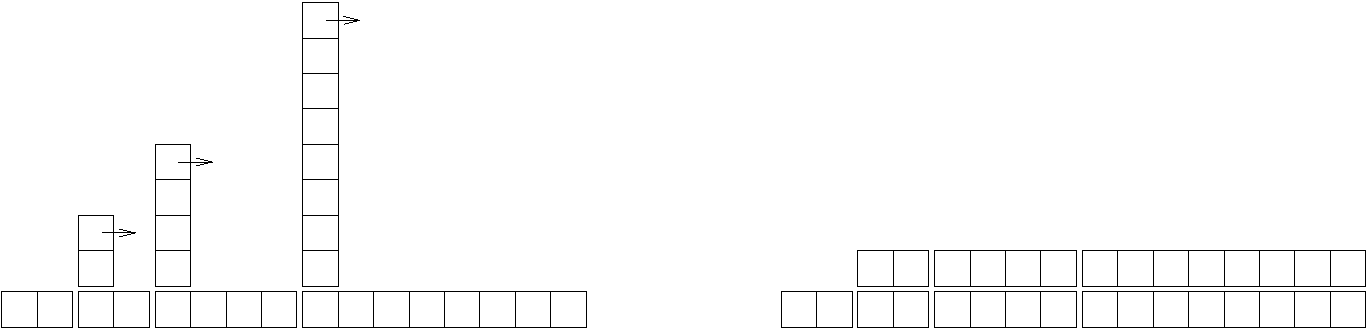
\includegraphics[scale=1.0]{figs/towers.pdf}}
\caption{Το κόστος μίας προσθήκης πίνακα κατακερματισμού.} 
\label{fig.hash}
\end{figure}

 Το επιπλέον έργο για τον επανακατακερματισμό εμφανίζεται σαν μία ακολουθία 
από όλο και υψηλότερους πύργους με όλο και μεγαλύτερα διαστήματα μεταξύ τους.  Τώρα, αν γκρεμίσετε τους πύργους, μοιράζοντας το κόστος σε όλες τις προσθήκες, θα δείτε γραφικά ότι το συνολικό κόστος μετά από $n$ προσθήκες είναι $2n - 2$.

Ένα σημαντικό χαρακτηριστικό αυτού του αλγορίθμου είναι ότι όταν αλλάζουμε το μέγεθος του πίνακα κατακερματισμού τότε αυξάνεται γεωμετρικά. Ήτοι πολλαπλασιάζουμε το μέγεθος με μια σταθερά.  Αν αυξήσετε το μέγεθος αριθμητικώς (προσθέτοντας ένα συγκεκριμένο αριθμό κάθε φορά), ο μέσος χρόνος για κάθε  {\tt add}  είναι γραμμικός.
\index{geometric resizing}

Μπορείτε να κατεβάσετε την υλοποίηση μου για την  HashMap  από εδώ  
\url{http://thinkpython/code/Map.py},  αλλά θυμηθείτε ότι δεν υπάρχει λόγος να την χρησιμοποιήσετε. Αν θέλετε να αντιστοιχίσετε τότε μπορείτε απλά να χρησιμοποιήσετε ένα λεξικό της  Python.





\chapter{Lumpy}
\label{lumpy}

 
Καθ'όλη τη διάρκεια του βιβλίου, έχω χρησιμοποιήσει διαγράμματα για να αναπαραστήσω την κατάσταση των προγραμμάτων που εκτελούνται.
\index{Lumpy}

Στην Ενότητα~\ref{variables}, χρησιμοποιήσαμε ένα διάγραμμα κατάστασης για να καταδείξουμε τα ονόματα και τις τιμές των μεταβλητών.  Στην Ενότητα~\ref{stackdiagram} παρουσίασα ένα διάγραμμα κατάστασης στο οποίο κάθε κλήση συνάρτησης αναπαριστάται από ένα πλαίσιο.  Κάθε πλαίσιο δείχνει τις παραμέτρους και 
τις τοπικές μεταβλητές για κάθε συνάρτηση ή μέθοδο.  Τα διαγράμματα κατάστασης για τις αναδρομικές συναρτήσεις φαίνονται στην Ενότητα~\ref{recursive.stack} και στην 
Ενότητα~\ref{more.recursion}.
\index{stack diagram} \index{diagram!stack}
\index{state diagram} \index{diagram!state}

Η Ενότητα~\ref{mutable} δείχνει πως φαίνεται μία λίστα σε ένα διάγραμμα κατάστασης, 
η Ενότητα~\ref{invert} δείχνει πως φαίνεται ένα λεξικό και η Ενότητα~\ref{dictuple} 
δείχνει δύο τρόπους για την αναπαράσταση των πλειάδων.

Στην Ενότητα~\ref{attributes} παρουσιάζονται τα διαγράμματα αντικειμένων, τα οποία 
δείχνουν την κατάσταση των ιδιοτήτων ενός αντικειμένου, των ιδιοτήτων αυτών των ιδιοτήτων και ούτω καθεξής.  Η Ενότητα~\ref{rectangles} έχει διαγράμματα αντικειμένων για τα ορθογώνια  (Rectangles)  και τα ενσωματωμένα σημεία τους  Points.   Η Ενότητα~\ref{time.object} δείχνει την κατάσταση ενός αντικειμένου ώρας  (Time). 
Η Ενότητα~\ref{class.attribute} έχει ένα διάγραμμα το οποίο περιέχει ένα αντικείμενο κλάσης και ένα στιγμιότυπο, τα καθένα με τις ιδιότητές του.
\index{object diagram}
\index{diagram!object}

Τέλος, στην Ενότητα~\ref{class.diagram} παρουσιάζονται τα διαγράμματα κλάσεων, τα οποία δείχνουν τις κλάσεις που συνθέτουν ένα πρόγραμμα και τις σχέσεις μεταξύ τους.
\index{class diagram}
\index{diagram!class}

Αυτά τα διαγράμματα βασίζονται στην  UML (Unified Modeling Language),  η οποία αποτελεί μία πρότυπη γλώσσα γραφικής απεικόνισης.  Η  UML  χρησιμοποιείται από τους μηχανικούς λογισμικού για να συνεννοούνται σχετικά με το σχεδιασμό του προγράμματος, ειδικά για τα αντικειμενοστραφή προγράμματα.
\index{Unified Modeling Language}
\index{UML}

Είναι μία πλούσια γλώσσα με πολλά είδη διαγραμμάτων τα οποία αναπαριστούν σχέσεις 
μεταξύ αντικειμένων και κλάσεων.  Σε αυτό το βιβλίο παρουσίασα μόνο ένα μικρό υποσύνολο της γλώσσας, αλλά αυτό είναι και το υποσύνολο που χρησιμοποιείται συνήθως στην πράξη.


Σκοπός αυτού του παραρτήματος είναι η ανασκόπηση των διαγραμμάτων που παρουσιάστηκαν στα προηγούμενα κεφάλαια και η εισαγωγή στη  Lumpy.   Η  
Lumpy,  η οποία σημαίνει  "UML in Python"  με λίγο αναγραμματισμό, είναι 
μέρος του  Swampy,  το οποίο έχετε ήδη εγκαταστήσει αν δουλέψατε στην μελέτη περίπτωσης του Κεφαλαίου~\ref{turtlechap} ή του Κεφαλαίου~\ref{tkinter}, ή αν κάνατε την Άσκηση~\ref{canvas}.
\index{Lumpy}
\index{Swampy}

Η  Lumpy  χρησιμοποιεί το άρθρωμα  {\tt inspect}  της  Python  για να εξετάσει την κατάσταση ενός προγράμματος που εκτελείται και να παράξει διαγράμματα αντικειμένων (συμπεριλαμβανομένων των διαγραμμάτων κατάστασης) και 
διαγράμματα κλάσεων.


\section{Διάγραμμα κατάστασης}

\begin{figure}
\centerline
{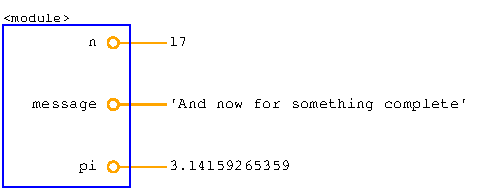
\includegraphics[scale=0.7]{figs/lumpydemo1.pdf}}
\caption{Διάγραμμα κατάστασης που δημιουργείται από την  Lumpy.} 
\label{fig.lumpy1}
\end{figure}

Αυτό είναι ένα παράδειγμα το οποίο χρησιμοποιεί την  Lumpy  για να δημιουργήσει ένα διάγραμμα κατάστασης.
\index{state diagram} \index{diagram!state} 

\begin{verbatim}
from swampy.Lumpy import Lumpy

lumpy = Lumpy()
lumpy.make_reference()

message = 'And now for something completely different'
n = 17
pi = 3.1415926535897932

lumpy.object_diagram()
\end{verbatim}

Η πρώτη γραμμή εισάγει την κλάση  Lumpy  από το  {\tt swampy.Lumpy}.  
Αν δεν έχετε εγκαταστήσει το  Swampy  σαν πακέτο, σιγουρευτείτε ότι τα αρχεία του  Swampy  βρίσκονται στην διαδρομή αναζήτησης της  Python  και χρησιμοποιήστε αυτή τη δήλωση  {\tt import}:

\begin{verbatim}
from Lumpy import Lumpy
\end{verbatim}

 Οι επόμενες γραμμές δημιουργούν ένα αντικείμενο  {\tt Lumpy}  και φτιάχνουν ένα σημείο αναφοράς, το οποίο σημαίνει ότι η  Lumpy  καταγράφει 
τα αντικείμενα που έχουν οριστεί μέχρι στιγμής.

Στη συνέχεια ορίζουμε νέες μεταβλητές και επικαλούμαστε την \verb"object_diagram", η οποία σχεδιάζει τα αντικείμενα που έχουν οριστεί από 
το σημείο αναφοράς, σε αυτήν την περίπτωση τα  {\tt message}, {\tt n}  και  {\tt pi}.

 Η Εικόνα~\ref{fig.lumpy1}  δείχνει το αποτέλεσμα. Τα γραφικά είναι διαφορετικά από αυτά που έδειξα νωρίτερα.  Για παράδειγμα, κάθε αναφορά αναπαριστάται από έναν κύκλο δίπλα στο όνομα της μεταβλητής και μία γραμμή προς 
στην τιμή.  Και οι μεγάλες συμβολοσειρές είναι περικομμένες.  Αλλά η πληροφορία που παρέχει το διάγραμμα είναι η ίδια.

Τα ονόματα των μεταβλητών είναι σε ένα πλαίσιο με ετικέτα  \verb"<module>",  
το οποίο υποδεικνύει ότι αυτές είναι μεταβλητές του αρθρώματος, γνωστές και ως καθολικές.
\index{global variable}
\index{variable!global}
\index{module-level variable}
\index{variable!module-level}

Μπορείτε να κατεβάσετε αυτό το παράδειγμα από εδώ : 
\url{http://thinkpython.com/code/lumpy_demo1.py}.   
Δοκιμάστε να προσθέσετε μερικές επιπλέον εκχωρήσεις και δείτε πως θα φαίνεται το διάγραμμα.



\section{Διάγραμμα στοίβας}

\begin{figure}
\centerline
{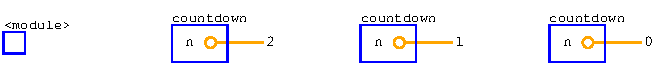
\includegraphics[scale=0.7]{figs/lumpydemo2.pdf}}
\caption{Διάγραμμα στοίβας.}
\label{fig.lumpy2}
\end{figure}

Αυτό είναι ένα παράδειγμα που χρησιμοποιεί την  Lumpy  για να δημιουργήσει 
ένα διάγραμμα στοίβας.  Μπορείτε να το κατεβάσετε από εδώ :
\url{http://thinkpython.com/code/lumpy_demo2.py}.
\index{stack diagram} \index{diagram!stack}

\begin{verbatim}
from swampy.Lumpy import Lumpy

def countdown(n):
    if n <= 0:
        print 'Blastoff!'
        lumpy.object_diagram()
    else:
        print n
        countdown(n-1)

lumpy = Lumpy()
lumpy.make_reference()
countdown(3)
\end{verbatim}

 Η Εικόνα~\ref{fig.lumpy2} δείχνει το αποτέλεσμα.  Κάθε πλαίσιο αναπαριστάται 
από ένα κουτί το οποίο έχει το όνομα της συνάρτησης απέξω και τις μεταβλητές στο 
εσωτερικό του.  Αφού αυτή η συνάρτηση είναι αναδρομική, υπάρχει ένα πλαίσιο για κάθε επίπεδο της αναδρομής.
\index{recursion}
\index{function frame}
\index{frame}

Θυμηθείτε ότι ένα διάγραμμα στοίβας δείχνει την κατάσταση του προγράμματος σε ένα 
συγκεκριμένο σημείο της εκτέλεσής του.  Για να πάρετε το διάγραμμα που θέλετε, μερικές φορές πρέπει να σκεφτείτε που πρέπει να επικαλεστείτε την   
\verb"object_diagram".

 Σε αυτήν την περίπτωση την επικαλέστηκα μετά την εκτέλεση της περίπτωσης βάσης της αναδρομής.  Με αυτόν τον τρόπο το διάγραμμα στοίβας δείχνει όλα τα επίπεδα της αναδρομής.  Μπορείτε να καλέσετε την \verb"object_diagram" περισσότερες από μία φορές ούτως ώστε να πάρετε μία σειρά από στιγμιότυπα της εκτέλεσης του προγράμματος.
\index{base case}


\section{Διαγράμματα αντικειμένων}

\begin{figure}
\centerline
{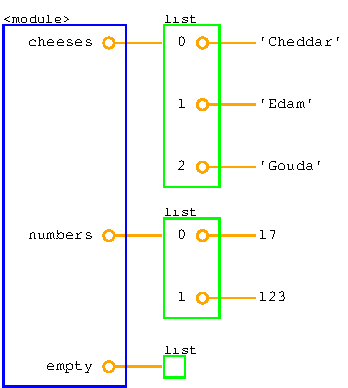
\includegraphics[scale=0.7]{figs/lumpydemo3.pdf}}
\caption{Διάγραμμα αντικειμένων.}
\label{fig.lumpy3}
\end{figure}

Αυτό το παράδειγμα παράγει ένα διάγραμμα αντικειμένου το οποίο δείχνει τις λίστες 
της Ενότητας~\ref{sequence}.  Μπορείτε να το κατεβάσετε από εδώ : 
\url{http://thinkpython.com/code/lumpy_demo3.py}.
\index{object diagram} \index{diagram!object}

\begin{verbatim}
from swampy.Lumpy import Lumpy

lumpy = Lumpy()
lumpy.make_reference()

cheeses = ['Cheddar', 'Edam', 'Gouda']
numbers = [17, 123]
empty = []

lumpy.object_diagram()
\end{verbatim}

 Η Εικόνα~\ref{fig.lumpy3} δείχνει το αποτέλεσμα.  Οι λίστες αναπαριστώνται 
από ένα κουτί το οποίο δείχνει τους δείκτες να αντιστοιχίζονται στα στοιχεία.  Αυτή 
η αναπαράσταση είναι ελαφρώς παραπλανητική, αφού οι δείκτες δεν είναι μέρος της λίστας στην πραγματικότητα, αλλά θεωρώ ότι κάνουν ευκολότερη την ανάγνωση του διαγράμματος.  Η κενή λίστα αναπαριστάται από ένα άδειο κουτί.
\index{list index}

\begin{figure}
\centerline
{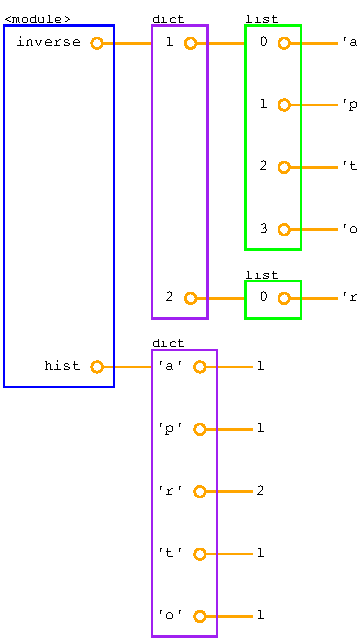
\includegraphics[scale=0.7]{figs/lumpydemo4.pdf}}
\caption{Διάγραμμα αντικειμένων.}
\label{fig.lumpy4}
\end{figure}

Και αυτό είναι ένα παράδειγμα το οποίο δείχνει τα λεξικά από την Ενότητα~\ref{invert}.  Μπορείτε να το κατεβάσετε από εδώ : 
\url{http://thinkpython.com/code/lumpy_demo4.py}.
\index{dictionary}

\begin{verbatim}
from swampy.Lumpy import Lumpy

lumpy = Lumpy()
lumpy.make_reference()

hist = histogram('parrot')
inverse = invert_dict(hist)

lumpy.object_diagram()
\end{verbatim}

 Η Εικόνα~\ref{fig.lumpy4} δείχνει το αποτέλεσμα.  Το  {\tt hist}  είναι ένα λεξικό το οποίο αντιστοιχεί χαρακτήρες (συμβολοσειρές με ένα γράμμα) σε ακέραιους αριθμού.  Το  {\tt inverse}  αντιστοιχεί ακέραιους σε λίστες συμβολοσειρών.

\begin{figure}
\centerline
{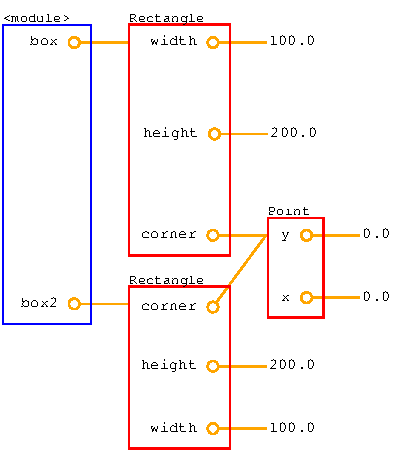
\includegraphics[scale=0.7]{figs/lumpydemo5.pdf}}
\caption{Διάγραμμα αντικειμένων.}
\label{fig.lumpy5}
\end{figure}

Αυτό το παράδειγμα παράγει ένα διάγραμμα αντικειμένων για αντικείμενα  Point  και  Rectangle,  όπως στην Ενότητα~\ref{copying}.  Μπορείτε να το κατεβάσετε από εδώ : \url{http://thinkpython.com/code/lumpy_demo5.py}.
\index{Point class}
\index{class!Point}
\index{Rectangle class}
\index{class!Rectangle}

\begin{verbatim}
import copy
from swampy.Lumpy import Lumpy

lumpy = Lumpy()
lumpy.make_reference()

box = Rectangle()
box.width = 100.0
box.height = 200.0
box.corner = Point()
box.corner.x = 0.0
box.corner.y = 0.0

box2 = copy.copy(box)

lumpy.object_diagram()
\end{verbatim}

 Η Εικόνα~\ref{fig.lumpy5} δείχνει το αποτέλεσμα.  Η  {\tt copy.copy}  κάνει μία ρηχή αντιγραφή, έτσι τα  {\tt box}  και  {\tt box2}  έχουν 
τα δικά τους  {\tt width}  και  {\tt height},  αλλά μοιράζονται το ίδιο ενσωματωμένο αντικείμενο  Point.   Αυτού του είδους η κοινή χρήση είναι συνήθως εντάξει με αμετάβλητα αντικείμενα, αλλά είναι πολύ επιρρεπή σε λάθη με μεταβλητούς τύπους.
\index{copy}
\index{shallow copy}

\section{Αντικείμενα συναρτήσεων και κλάσεων}

\begin{figure}
\centerline
{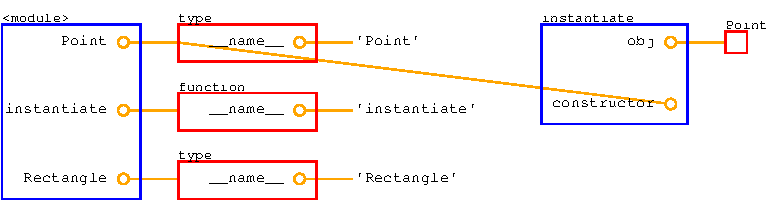
\includegraphics[scale=0.7]{figs/lumpydemo6.pdf}}
\caption{Διάγραμμα αντικειμένων.}
\label{fig.lumpy6}
\end{figure}

Συνήθως, όταν χρησιμοποιώ την  Lumpy  για να φτιάξω διαγράμματα αντικειμένων, ορίζω τις συναρτήσεις και τις κλάσεις προτού φτιάξω το σημείο αναφοράς.  Με αυτόν τον τρόπο, τα αντικείμενα των συναρτήσεων και των κλάσεων δεν εμφανίζονται μέσα στο διάγραμμα.
\index{function object}
\index{object!function}
\index{class object}
\index{object!class}

Αλλά αν περάσετε τις συναρτήσεις και τις κλάσεις σαν παραμέτρους, ίσως θέλατε και να εμφανίζονται.  Αυτό είναι ένα παράδειγμα το οποίο μπορείτε να κατεβάσετε από εδώ : \url{http://thinkpython.com/code/lumpy_demo6.py}. 

\begin{verbatim}
import copy
from swampy.Lumpy import Lumpy

lumpy = Lumpy()
lumpy.make_reference()

class Point(object):
    """Represents a point in 2-D space."""

class Rectangle(object):
    """Represents a rectangle."""

def instantiate(constructor):
    """Instantiates a new object."""
    obj = constructor()
    lumpy.object_diagram()
    return obj

point = instantiate(Point)
\end{verbatim}

Η Εικόνα~\ref{fig.lumpy6} δείχνει το αποτέλεσμα.  Αφού επικαλεστήκαμε την  
\verb"object_diagram"  μέσα σε μία συνάρτηση, θα πάρουμε ένα διάγραμμα στοίβας 
με ένα πλαίσιο για τις καθολικές μεταβλητές και για τις επικλήσεις της  
{\tt instantiate}.

 Στο επίπεδο αρθρώματος, τα  {\tt Point}  και  {\tt Rectangle}  αναφέρονται σε αντικείμενα κλάσεων (τα οποία έχουν τύπο  {\tt type} ) και το 
 {\tt instantiate}  αναφέρεται σε ένα αντικείμενο συνάρτησης.
\index{instantiate}
\index{constructor}

Αυτό το διάγραμμα μπορεί να αποσαφηνίσει δύο από συνηθέστερα σημεία σύγχυσης :  (1) τη διαφορά μεταξύ του αντικειμένου κλάσης,  {\tt Point},  και του στιγμιότυπου ενός  Point, {\tt obj},  και (2) τη διαφορά μεταξύ του αντικειμένου συνάρτησης που δημιουργήθηκε όταν ορίστηκε η  {\tt instantiate}  και του πλαισίου που δημιουργήθηκε όταν καλέστηκε αυτή.



\section{Διαγράμματα Κλάσεων}

\begin{figure}
\centerline
{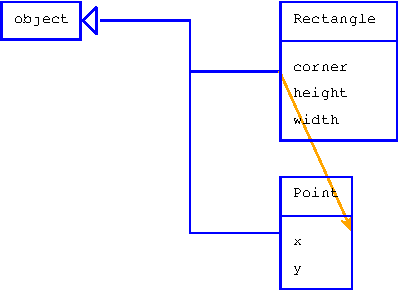
\includegraphics[scale=0.7]{figs/lumpydemo7.pdf}}
\caption{Διάγραμμα κλάσεων.}
\label{fig.lumpy7}
\end{figure}

\begin{figure}
\centerline
{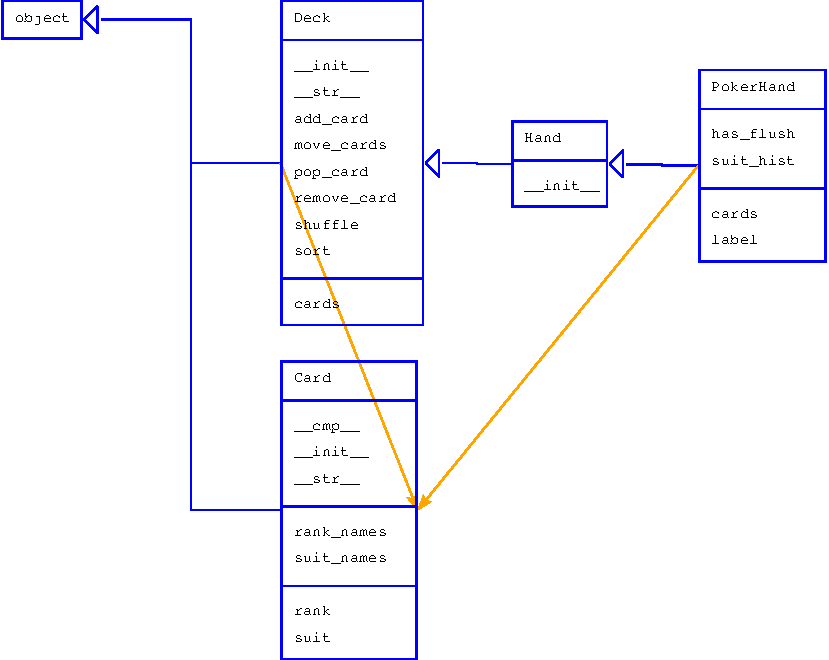
\includegraphics[scale=0.7]{figs/lumpydemo8.pdf}}
\caption{Διάγραμμα κλάσεων.}
\label{fig.lumpy8}
\end{figure}

Παρά το γεγονός ότι έκανα διάκριση μεταξύ των διαγραμμάτων κατάστασης, στοίβας και αντικειμένων, είναι επί το πλείστον το ίδιο πράγμα :  δείχνουν την κατάσταση ενός προγράμματος που εκτελείται σε μία δεδομένη χρονική στιγμή.
\index{class diagram}
\index{diagram!class}

Τα διαγράμματα κλάσεων είναι διαφορετικά.  Δείχνουν τις κλάσεις που συνθέτουν ένα πρόγραμμα και τις σχέσεις μεταξύ τους.  Είναι διαχρονικές υπό την έννοια ότι περιγράφουν το πρόγραμμα στο σύνολο του, όχι σε μία συγκεκριμένη χρονική στιγμή.  
Για παράδειγμα, αν ένα στιγμιότυπο της κλάσης Α γενικά μία αναφορά σε ένα στιγμιότυπο της κλάσης Β, τότε λέμε ότι υπάρχει μία σχέση  " ΕΧΕΙ-ΕΝΑ "  μεταξύ αυτών των κλάσεων.
\index{HAS-A relationship}
\index{class diagram}
\index{diagram!class}
\index{UML}

Αυτό είναι ένα παράδειγμα το οποίο δείχνει μία σχέση ΕΧΕΙ-ΕΝΑ.  Μπορείτε να το κατεβάσετε από εδώ : \url{http://thinkpython.com/code/lumpy_demo7.py}.

\begin{verbatim}
from swampy.Lumpy import Lumpy

lumpy = Lumpy()
lumpy.make_reference()

box = Rectangle()
box.width = 100.0
box.height = 200.0
box.corner = Point()
box.corner.x = 0.0
box.corner.y = 0.0

lumpy.class_diagram()
\end{verbatim}

 Η Εικόνα~\ref{fig.lumpy7} δείχνει το αποτέλεσμα. Κάθε κλάση αναπαριστάται με ένα κουτί το οποίο περιέχει το όνομα της συνάρτησης, όλες μεθόδους που παρέχει η κλάση, όλες τις μεταβλητές της κλάσης και όλα τα μεταβλητές των στιγμιοτύπων, αλλά όχι μεθόδους και μεταβλητές κλάσεων.

Το βέλος από η  {\tt Rectangle}  στην  {\tt Point}  δείχνει ότι τα ορθογώνια περιέχουν ένα ενσωματωμένο σημείο.  Επιπλέον, τόσο η  {\tt Rectangle}  όσο και η  {\tt Point}  κληρονομούν την  {\tt object},  η οποία αναπαριστάται στο διάγραμμα από ένα βέλος με τριγωνάκι στην κεφαλή του.
\index{IS-A relationship}

Αυτό είναι ένα πιο σύνθετο παράδειγμα στο οποίο χρησιμοποιώ την λύση μου για την Άσκηση~\ref{poker}.  Μπορείτε να κατεβάσετε τον κώδικα από εδώ :  \url{http://thinkpython.com/code/lumpy_demo8.py}.   Θα χρειαστείτε επίσης και το  : \url{http://thinkpython.com/code/PokerHand.py}.

\begin{verbatim}
from swampy.Lumpy import Lumpy

from PokerHand import *

lumpy = Lumpy()
lumpy.make_reference()

deck = Deck()
hand = PokerHand()
deck.move_cards(hand, 7)

lumpy.class_diagram()
\end{verbatim}

 Η Εικόνα~\ref{fig.lumpy8} δείχνει το αποτέλεσμα. Η  {\tt PokerHand}  κληρονομεί την  {\tt Deck}.   Και η  {\tt Deck}  και η  {\tt PokerHand}  έχουν τραπουλόχαρτα.
\index{Card class}
\index{Deck class}
\index{Hand class}

Αυτό το διάγραμμα δεν δείχνει ότι και η  {\tt Hand}  έχει τραπουλόχαρτα, επειδή δεν υπάρχουν στιγμιότυπα της  Hand  στο πρόγραμμα.  Αυτό το παράδειγμα 
καταδεικνύει έναν περιορισμό της  Lumpy.   Η  Lumpy  γνωρίζει μόνο τις ιδιότητες και τις σχέσεις ΕΧΕΙ-ΕΝΑ των αντικειμένων τα οποία έχουν αρχικοποιηθεί.

 
\printindex
%\blankpage
%\blankpage
%\blankpage


\end{document}
